\documentclass[leqno,b5paper]{book}
%\documentclass[leqno]{book} %the geometry package defines the paper size
%===================
%testing tikz inside book
\usepackage{circuitikz}
\usepackage{pgfplotstable}
\usepackage{pgfplots}

\usepackage{tikz-3dplot}
\pgfplotsset{compat=newest,}
\usepgfplotslibrary{units}
%\pgfplotsset{compat=1.9}
\usepgfplotslibrary{polar}
\usepackage{ifdraft}
\usepackage{multicol}                                        %for getting multicolumn itemize, enumerate etc
\usepackage{enumerate}                   %for getting better auto numbering in enumerate

%pathmorphing gives the ripples like look
\usetikzlibrary{3d,shadings,fadings,intersections,calc,decorations.markings,decorations.pathreplacing,external,shapes.misc,decorations.pathmorphing,patterns}


%\tikzexternalize[mode=list and make] %disable to generate figures
%\tikzexternaldisable  %enables figures after this command. put this is the tex file

\usepackage{scrextend}   % \begin{labeling}{}  \end{labeling}   just like Description
%for vertical spacing in tables use\Tstrut and \Bstrut  
\newcommand\Tstrut{\rule{0pt}{2.6ex}}       % Top strut
\newcommand\Bstrut{\rule[-1.2ex]{0pt}{0pt}} % Bottom strut

\definecolor{lgray}{cmyk}{0,0,0,0.2}
\definecolor{dgray}{cmyk}{0,0,0,0.7}
%========================
%\usepackage[hidelinks]{hyperref}  %used in machines book but not here
\usepackage{./tex/khalidUrduBooksMaths}                     %my sty file
\usepackage{amsbsy} %for bold Poynting, lessgtr symbol
\usepackage{mathrsfs}   %for Poynting symbol
\usepackage{IEEEtrantools}
\usepackage{multirow}   %for multiple row cells in a table column
\usepackage[misc]{ifsym} 

\newtagform{brackets}{)}{(}   			%mathtools command to correct braces around equation numbers
\usetagform{brackets}				%had to do this after ubuntu upgrade messed up braces around eq numbers.
 
\newcommand*{\kStrokeOne}{|}                                      %tally marks (statistics)
\newcommand*{\kStrokeTwo}{|\!|}
\newcommand*{\kStrokeThree}{|\!|\!|}
\newcommand*{\kStrokeFour}{|\!|\!|\!|}
\newcommand*{\kStrokeFive}{\cancel\kStrokeFour}

\sisetup{math-micro=\textup{µ},text-micro=µ,math-ohm  =\upOmega}   %with mathpazo this is needed else must not be here. now micro is smaller
\DeclareSIUnit \var {var}    %used in electric circuits volt-ampere-reactive

\input longdiv.tex
\usepackage{polynom}
\usepgfplotslibrary{fillbetween}


%this file describes urdu commands for the commonly used english latex commands

%chapter, section etc
%  \newcommand*{newcommand}[arguments]{actual command}
\newcommand*{\باب}[1]{\chapter{#1}}                                      %defining commonly used commands
\newcommand*{\حصہ}[1]{\section{#1}}
\newcommand*{\جزوحصہ}[1]{\subsection{#1}}
\newcommand*{\جزوجزوحصہ}[1]{\subsubsection{#1}}

\newcommand*{\بابء}[1]{\chapter*{#1}}                                      %defining commonly used commands
\newcommand*{\حصہء}[1]{\section*{#1}}
\newcommand*{\جزوحصہء}[1]{\subsection*{#1}}
\newcommand*{\جزوجزوحصہء}[1]{\subsubsection*{#1}}


%english text in urdu mode
\newcommand*{\تحریر}[1]{\textenglish{#1}}	% english text in urduMode
%\newcommand*{\موٹا}[1]{\textbf{#1}}
%\newcommand*{\ترچھا}[1]{{\textit{#1}}}
\newcommand*{\موٹا}[1]{{\urduTechTermsfont{#1}}}
%\newcommand*{\ترچھا}[1]{{\urduTechTermsfont{#1}}}
\newcommand*{\ترچھا}[1]{{\small{#1}}}

%\newcommand*{\اصطلاح}[1]{{\color{red}{#1}}}   %colours spills to next word when there is index or footnote entry with the word
%\newcommand{\اصطلاح}[1]{{\urdufontBig{#1}}}
\newcommand{\اصطلاح}[1]{{\urduTechTermsfont{#1}}}


%end commands cannot be redefined and as such these two are not usable
\providecommand*{\ابتدا}[1]{\begin{#1}}
\providecommand*{\انتہا}[1]{\end{#1}}

%include and input directives for adding external files into the main document 
\newcommand*{\بشمول}[1]{\includeonly{#1}}
\newcommand*{\شامل}[1]{\include{#1}}
\newcommand*{\داخل}[1]{\input{#1}}

%to use extra latex packages
\newcommand*{\استعمال}[1]{\usepackage{#1}}

%footnotes and indexes
\newcommand*{\حاشیہب}[1]{{\raggedright{\footnote{\textenglish{#1}}}} }               %footnote to the left hand side
\newcommand*{\حاشیہد}[1]{{\raggedleft{\footnote{#1}}}}
\newcommand*{\حاشیہط}[1]{\marginpar{#1}}

\newcommand*{\فرہنگ}[1]{\index{#1}}

%references and labels
\newcommand*{\شناخت}[1]{\label{#1}}
\newcommand*{\حوالہ}[1]{\ref{#1}}
\newcommand*{\حوالہصفحہ}[1]{\pageref{#1}}

%counters
\newcommand*{\فاصلہ}{\vspace*{10mm}}
\newcommand*{\فاصلہء}{\quad}

%itemize, bullets and numbered items   
\newcommand*{\اشیاء}{itemize}                               %used in   \begin{itemize}
\newcommand*{\شے}[1]{\item {#1}}			%used in    \item, \description
%description
\newcommand*{\جزو}[1]{\item[#1]}                      %used in \begin{description}
%maths commands
\newcommand*{\عددی}[1]{\: \ensuremath{#1} \:} % in-line math & inside math mode
\newcommand*{\عددیء}[1]{\ensuremath{#1}}
\newcommand*{\سمتیہ}[1]{\ensuremath{{\bf{#1}}}}
\newcommand*{\سمتیازیرنوشت}[2]{\ensuremath{{\boldsymbol{#1}}_{\textup{#2}}}}

\newcommand*{\ضرب}{\time}					%multiplication symbol
\newcommand*{\نکطہد}{\cdot}
\newcommand*{\نقطے}{\ensuremath{\cdots}}

\newcommand*{\زیرنوشت}[3]{\: \ensuremath{{#1_{#2 \textrm {#3}}}} \:}   %english+urdu subscript \زیرنوشت{V}{CE}{غیرافزائندہ}
\newcommand*{\سیدھازیرنوشت}[2]{\: \ensuremath{{#1_{\textup{#2}}}} \:} %RC

\newcommand*{\قریب}[1]{\mbox{#1}}
\newcommand{\سن}[1]{؁\,\ensuremath{#1}}


\renewcommand{\indexname}{فرہنگ}        %does nothing here. must be placed within begin{urdufont} environment to be the last to take effect 
%===============================


%numbering scheme
\renewcommand*{\thefigure}{\arabic{figure}.\thechapter}
\renewcommand*{\thetable}{\arabic{table}.\thechapter}
\renewcommand*{\theequation}{\arabic{equation}.\thechapter}
\renewcommand*{\thesection}{\arabic{section}.\thechapter}
\renewcommand*{\thesubsection}{\arabic{subsection}.\arabic{section}.\thechapter}
\renewcommand*{\thesubsubsection}{\arabic{subsubsection}.\arabic{subsection}.\arabic{section}.\thechapter}
%=======================================
%the following pertains to theorem environment. added to maths sty
\renewcommand*{\thetheorem}{\arabic{theorem}.\thechapter}
\renewcommand*{\thecorollary}{\arabic{corollary}.\arabic{theorem}.\thechapter}
\renewcommand*{\thelemma}{\arabic{lemma}.\thechapter}
\renewcommand*{\thedefinition}{\arabic{definition}.\thechapter}


%================
%my environments
%================

%environment for examples مثال
%\newcounter{examplecounter}[section]
%\renewcommand{\theexamplecounter}{\arabic{examplecounter}}
\newcounter{examplecounter}[chapter]
\renewcommand{\theexamplecounter}{\arabic{examplecounter}.\thechapter}

\newenvironment*{مثال}
{\par\noindent\ignorespaces    مثال \refstepcounter{examplecounter} \theexamplecounter :\quad}%
{\hfill\qedsymbol  \vspace{\baselineskip}\par}
%{\noindent\ignorespaces \vspace{\baselineskip} \hrule \vspace{\baselineskip}  مثال \refstepcounter{examplecounter} \theexamplecounter :}%
%{\par\noindent \hrule  \vspace{\baselineskip}}

%------
%practice problems environment مشق

%\newcounter{practicecounter}[section]                              %practice here means مشق
%\renewcommand{\thepracticecounter}{\arabic{practicecounter}}
\newcounter{practicecounter}[chapter]                              %practice here means مشق
\renewcommand{\thepracticecounter}{\arabic{practicecounter}.\thechapter}

\newenvironment*{مشق}
{\par\noindent\ignorespaces \vspace{\baselineskip} \hrule \vspace{\baselineskip} مشق \refstepcounter{practicecounter} \thepracticecounter :\quad}%
{\par\noindent \hrule  \vspace{\baselineskip}}
%---------

%end of chapter questions environment سوال

\newcounter{questioncounter}[section]
\renewcommand{\thequestioncounter}{\arabic{questioncounter}}
%\newcounter{questioncounter}[chapter]
%\renewcommand{\thequestioncounter}{\arabic{questioncounter}.\thechapter}

\newenvironment*{سوال}				
{\noindent\ignorespaces  سوال \refstepcounter{questioncounter} \thequestioncounter :\quad}%
{\par\noindent }
%--------------------

%defining a LAW   قانون

%\newcounter{lawcounter}[section]
%\renewcommand{\thelawcounter}{\arabic{lawcounter}}
\newcounter{lawcounter}[chapter]
\renewcommand{\thelawcounter}{\arabic{lawcounter}.\thechapter}

\newenvironment*{قانون}				
{\par\medskip \refstepcounter{lawcounter} }%
{\par\medskip }
%--------------------
%--------------------

%defining a THEOREM   مسئلہ

%\newcounter{kthcounter}[section]
%\renewcommand{\thekthcounter}{\arabic{kthcounter}}
\newcounter{kthcounter}[chapter]
\renewcommand{\thekthcounter}{\arabic{kthcounter}.\thechapter}

\newenvironment*{مسئلہ}				
{\par\noindent\ignorespaces  مسئلہ \refstepcounter{kthcounter} \thekthcounter :\quad}%
{\par\noindent }
%--------------------
%--------------------

%defining a Proof   ثبوت

%\newcounter{kprcounter}[chapter]
%\renewcommand{\thekprcounter}{\arabic{kprcounter}.\thechapter}

\newenvironment*{ثبوت}				
{\noindent\ignorespaces  ثبوت :\quad}%
{\par\hfill\qedsymbol  \vspace{\baselineskip}\par }
%{\par\noindent\qedsymbol  \vspace{\baselineskip} }
%--------------------
%--------------------

%defining a Definition تعریف

%\newcounter{kdfcounter}[chapter]
%\renewcommand{\thedfrcounter}{\arabic{kdfcounter}.\thechapter}

\newenvironment*{تعریف}				
{\par\noindent\ignorespaces  تعریف :\quad}%
{\par\noindent }
%--------------------
%--------------------

%defining a Definition مفروضہ

%\newcounter{kAscounter}[chapter]
%\renewcommand{\theAsrcounter}{\arabic{kAscounter}.\thechapter}

\newenvironment*{مفروضہ}				
{\par\noindent\ignorespaces  مفروضہ \quad}%
{\par\noindent }
%--------------------
                  %turning latex into urdu
% Greek Letters for Urdu Latex usage

\newcommand*{\ایلفا}{\alpha}
\newcommand*{\بیٹا}{\beta}
\newcommand*{\گیما}{\gamma}
\newcommand*{\ڈیلٹا}{\delta}
\newcommand*{\ایپسلان}{\epsilon}
\newcommand*{\متغیرایپسلان}{\varepsilon}
\newcommand*{\زیٹا}{\zeta}
\newcommand*{\ایٹا}{\eta}
\newcommand*{\تھیٹا}{\theta}
\newcommand*{\متغیرتھیٹا}{\vartheta}
\newcommand*{\ایوٹا}{\iota}
\newcommand*{\کاپا}{\kappa}
\newcommand*{\لیمڈا}{\lambda}
\newcommand*{\میو}{\mu}
\newcommand*{\نیو}{\nu}
\newcommand*{\ژاے}{\xi}
\newcommand*{\پاے}{\pi}
\newcommand*{\متغیرپاے}{\varpi}
\newcommand*{\رھو}{\rho}
\newcommand*{\متغیررھو}{\varrho}
\newcommand*{\سگما}{\sigma}
\newcommand*{\متغیرسگما}{\varsigma}
\newcommand*{\ٹو}{\tau}
\newcommand*{\اپسیلان}{\upsilon}
\newcommand*{\فاے}{\phi}
\newcommand*{\متغیفاے}{\varphi}
\newcommand*{\چاے}{\chi}
\newcommand*{\ساے}{\psi}
\newcommand*{\اومیگا}{\omega}

\newcommand*{\بڑاگیما}{\Gamma}
\newcommand*{\بڑاڈیلٹا}{\Delta}
\newcommand*{\بڑاتھیٹا}{\Theta}
\newcommand*{\بڑالیمڈا}{\Lambda}
\newcommand*{\بڑاژاے}{\Xi}
\newcommand*{\بڑاپاے}{\Pi}
\newcommand*{\بڑاسگما}{\Sigma}
\newcommand*{\بڑاساے}{\Psi}
\newcommand*{\بڑااومیگا}{\Omega}



\newcommand*{\kvec}[1]{{\ensuremath{{\boldsymbol{#1}}}}}
\newcommand*{\kvecsub}[2]{{\ensuremath{{\boldsymbol{#1}}}_{\textup{#2}}}}

\newcommand*{\ax}{\ensuremath{{\boldsymbol{a}}_{\textup{x}}}}
\newcommand*{\ay}{\ensuremath{{\boldsymbol{a}}_{\textup{y}}}}
\newcommand*{\az}{\ensuremath{{\boldsymbol{a}}_{\textup{z}}}}
%
\newcommand*{\arho}{\ensuremath{{\boldsymbol{a}}_{\rho}}}
\newcommand*{\aphi}{\ensuremath{{\boldsymbol{a}}_{\phi}}}
%
\newcommand*{\ar}{\ensuremath{{\boldsymbol{a}}_{\textup{r}}}}
\newcommand*{\atheta}{\ensuremath{{\boldsymbol{a}}_{\theta}}}

\newcommand*{\aN}{\ensuremath{{\boldsymbol{a}}_N}}
\newcommand*{\aR}{\ensuremath{{\boldsymbol{a}}_{\textup{R}}}}
\newcommand*{\aL}{\ensuremath{{\boldsymbol{a}}_{\textup{L}}}}

\newcommand*{\au}{\ensuremath{{\boldsymbol{a}}_u}}
\newcommand*{\av}{\ensuremath{{\boldsymbol{a}}_v}}
\newcommand*{\aw}{\ensuremath{{\boldsymbol{a}}_w}}

\newcommand*{\ai}{\ensuremath{{\boldsymbol{i}}}}
\newcommand*{\aj}{\ensuremath{{\boldsymbol{j}}}}
\newcommand*{\ak}{\ensuremath{{\boldsymbol{k}}}}


\newcommand*{\Ex}{\ensuremath{{\boldsymbol{E}}_x}}
\newcommand*{\Ey}{\ensuremath{{\boldsymbol{E}}_y}}
\newcommand*{\Ez}{\ensuremath{{\boldsymbol{E}}_z}}
%
\newcommand*{\Erho}{\ensuremath{{\boldsymbol{E}}_{\rho}}}
\newcommand*{\Ephi}{\ensuremath{{\boldsymbol{E}}_{\phi}}}
%
\newcommand*{\Er}{\ensuremath{{\boldsymbol{E}}_r}}
\newcommand*{\Etheta}{\ensuremath{{\boldsymbol{E}}_{\theta}}}

\newcommand*{\TE}[1]{\ensuremath{\textup{TE}_{#1}}}
\newcommand*{\TM}[1]{\ensuremath{\textup{TM}_{#1}}}
\newcommand*{\TEM}{\ensuremath{\textup{TEM}}}
%===========================
\newcommand{\RightAngle}[4][5pt]{\draw[gray] ($#3!#1!#2$)--($ #3!2!($($#3!#1!#2$)!.5!($#3!#1!#4$)$) $) --($#3!#1!#4$) ;        }



\DeclareMathOperator{\sech}{sech}
\DeclareMathOperator{\csch}{csch}
\DeclareMathOperator{\cosec}{cosec}
\DeclareMathOperator{\arcsec}{arcsec}
\DeclareMathOperator{\arccot}{arcCot}
\DeclareMathOperator{\arccsc}{arcCsc}
\DeclareMathOperator{\arccosine}{arcCos}
\DeclareMathOperator{\arccosh}{arcCosh}
\DeclareMathOperator{\arcsinh}{arcsinh}
\DeclareMathOperator{\arctanh}{arctanh}
\DeclareMathOperator{\arcsech}{arcsech}
\DeclareMathOperator{\arccsch}{arcCsch}
\DeclareMathOperator{\arccoth}{arcCoth} 
\DeclareMathOperator{\erf}{erf} 
\DeclareMathOperator{\erfc}{erfc} 
%the following two Sine Integral symbols doesnot clash with SI units package
\DeclareMathOperator{\kSi}{Si} 
\DeclareMathOperator{\ksi}{si} 
\DeclareMathOperator{\kS}{S} 
%cosine integral, exponential integral, logrithmic integral
\DeclareMathOperator{\ci}{ci} 
\DeclareMathOperator{\kC}{C} 
\DeclareMathOperator{\Ei}{Ei} 
\DeclareMathOperator{\li}{li} 
%Fresnel Cosine and SineIntegrals and their Auxiliary integrals
\DeclareMathOperator{\FC}{C} 
\DeclareMathOperator{\FS}{S} 
\DeclareMathOperator{\FAC}{c}                  %complementary Fresnel integral
\DeclareMathOperator{\FAS}{s}                     %complementary Fresnel integral
\DeclareMathOperator{\gammaQ}{Q}                     %Incomplete gamma function
\DeclareMathOperator{\gammaP}{P}                     %Incomplete gamma function
%Hermite polynomials
\DeclareMathOperator{\He}{He} 
%Complex Natural Logarithm, Principal Value
\DeclareMathOperator{\Ln}{Ln} 
%Residue 
\DeclareMathOperator{\Res}{Res}
%Lagrange interpolation formula
\DeclareMathOperator{\Lagrange}{L}
%statistics UpperControlLimit and Lower Control Limit, Average Outgoing Quality
\DeclareMathOperator{\UCL}{UCL} 
\DeclareMathOperator{\LCL}{LCL} 
\DeclareMathOperator{\CL}{CL} 
\DeclareMathOperator{\OC}{OC} 
\DeclareMathOperator{\AOQ}{AOQ} 
%projection of a vector
\DeclareMathOperator{\proj}{proj} 
     %\sech, \csch, \arcsh, \arcs   hyperbolic and arc-secant etc

\pgfmathsetmacro{\x}{2}     %smallest resistor sizes
\pgfmathsetmacro{\y}{2}
\pgfmathsetmacro{\xx}{2.5}   %somewhat larger resistor leads. gives more space
\pgfmathsetmacro{\yy}{2.5}
\pgfmathsetmacro{\xxx}{3}   %still larger resistor leads. gives even more space
\pgfmathsetmacro{\yyy}{3}
\pgfmathsetmacro{\dx}{0.2}     %moving labels beyond resistor outline
\pgfmathsetmacro{\dy}{0.2}
\pgfmathsetmacro{\pin}{0.3}

\pgfmathsetmacro{\boxW}{0.5}   %width of box circuit
\pgfmathsetmacro{\boxH}{2.5}   %height of box circuit

%=============================
%complex numbers, squared voltages
\newcommand*{\bZ}{{\ensuremath{{\boldsymbol{Z}}}}}           %complex impedance
\newcommand*{\bY}{{\ensuremath{{\boldsymbol{Y}}}}}           %complex admittance
\newcommand*{\bZCC}{{\ensuremath{{\boldsymbol{Z}}^{*}}}}                                            %complex conjugate impedance
\newcommand*{\bYCC}{{\ensuremath{{\boldsymbol{Y}}^{*}}}}                                            %complex conjugate

\newcommand*{\bVrms}{{\ensuremath{\hat{V}_{\textup{rms}}}}}           %phasor voltage
\newcommand*{\bIrms}{{\ensuremath{\hat{I}_{\textup{rms}}}}}           %phasor current
\newcommand*{\Vrms}{{\ensuremath{V_{\textup{rms}}}}}       %rms voltage
\newcommand*{\Irms}{{\ensuremath{I_{\textup{rms}}}}}           %rms current
\newcommand*{\Arms}{{\ensuremath{A_{\textup{rms}}}}}           %rms amps
\newcommand*{\VrmsS}{{\ensuremath{V^2_{\textup{rms}}}}}       %rms squared
\newcommand*{\IrmsS}{{\ensuremath{I^2_{\textup{rms}}}}}           %rms squared
\newcommand*{\bVrmsCC}{{\ensuremath{\hat{V}^{*}_{\textup{rms}}}}}                  %conjugate phasor voltage
\newcommand*{\bIrmsCC}{{\ensuremath{\hat{I}^{*}_{\textup{rms}}}}}           %conjugate phasor current


\newcommand*{\kx}[1]{{\ensuremath{{\boldsymbol{#1}}}}}                  %complex quantity
\newcommand*{\bS}{{\ensuremath{{\boldsymbol{S}}}}}                         %complex power
\newcommand*{\bH}{{\ensuremath{{\boldsymbol{H}}}}}                       %network functions
\newcommand*{\bA}{{\ensuremath{{\boldsymbol{A}}}}}                        %voltage gain

\newcommand*{\pf}{{\ensuremath{{\textup{pf}}}}}
\newcommand*{\rms}{{\ensuremath{\textup{rms}}}}           %rms
\newcommand*{\BW}{{\ensuremath{{\textup{BW}}}}}   %bandwidth

\newcommand*{\Laplace}{\mathcal{L}}   %Laplace transform
\newcommand*{\Fourier}{\mathcal{F}}   %Fourier transform

\newcommand*{\kB}[1]{{\ensuremath{{\textup{#1}}}}}  %Laplace symbol general use. 
									%following were used too often so gave them specific symbols
\newcommand*{\bF}{{\ensuremath{{\textup{F}}}}}    %Fourier transform of 
\newcommand*{\bP}{{\ensuremath{{\textup{P}}}}}   %Laplace fraction
\newcommand*{\bQ}{{\ensuremath{{\textup{Q}}}}}  %Laplace fraction
\newcommand*{\bV}{{\ensuremath{{\textup{V}}}}}  %Laplace Voltage
\newcommand*{\bI}{{\ensuremath{{\textup{I}}}}}  %Laplace Current
%Matrices and Vectors
\newcommand*{\bM}[1]{{\ensuremath{{\boldsymbol{#1}}}}} 
 % resistor sizes and Laplace, Fourier, Complex, Phasor, etc  symbols
%draws left and right arrows where needed e.g.  
% \draw[->-=0.5] (0,0)--(3,0); draws arrow at the middle
\tikzset{->-/.style={decoration={markings, mark=at position #1 with {\arrow{latex}}},postaction={decorate}}}
\tikzset{-<-/.style={decoration={markings, mark=at position #1 with {\arrow{latex reversed}}},postaction={decorate}}}
\tikzset{osquare/.style={draw,solid,fill=white, rectangle, minimum size=4pt, inner sep=0pt, outer sep=0pt}}   %node[osquare,fill=black]{}

%this puts small orthogonal tick marks along a curve at selected points. a point at each side of the location has to be provided to %the \path[] section of the command as shown.
% 		\draw[smooth, domain=0:2]plot ({\x},{\x^2});
%		\foreach \t in {0.5,1,1.5}{\path[| mark=0.5] ({\t-0.1},{(\t-0.1)^2}) -- ({\t+0.1},{(\t+0.1)^2});}
\tikzset{| mark/.style={postaction=decorate,decoration={markings,
mark=at position #1 with {\draw[line cap=round,mark segment] (0,-2pt) -- (0,2pt);
}}},mark segment/.style={thick}}


%draws right angles \RightAngle{A}{B}{C}
\providecommand{\RightAngle}[4][5pt]{\draw[] ($#3!#1!#2$)--($ #3!2!($($#3!#1!#2$)!.5!($#3!#1!#4$)$) $) --($#3!#1!#4$) ;     }
%colours
\definecolor{lgray}{cmyk}{0,0,0,0.2}
\definecolor{dgray}{cmyk}{0,0,0,0.7}
%draws a cross just like ocirc, circ; usage \fill(0,2)circle(1.5py);\draw(0,2)node[kcross]{};
\tikzset{kcross/.style={cross out, draw, 
         minimum size=2*(2pt-\pgflinewidth), 
         inner sep=0pt, outer sep=0pt}}


%tikz, pgfplot TABLE
\pgfplotsset{select coords between index/.style 2 args={
    x filter/.code={
        \ifnum\coordindex<#1\def\pgfmathresult{}\fi
        \ifnum\coordindex>#2\def\pgfmathresult{}\fi
    }
}}
%
%boxed circuits
%=========================================
%\leftBox[K]{3,2}   draws a box with lower end at (3,2) and the terminals called Ka and Kb
\newcommand{\boxLeft}[2][p]{
\coordinate (a) at (#2);
\draw (a)++(-0.025,0.5) coordinate (b);
\draw (a)++(-0.04,1) coordinate (c);
\draw (a)++(-0.12,1.5) coordinate (d);
\draw (a)++(-0.2,2) coordinate (e);
\draw (a)++(-0.15,2.5) coordinate (f);
\draw (a)++(0.5,3) coordinate (g);

\draw (a)++(0.7,2.5)coordinate(h);
\draw (a)++(0.6,2)coordinate(i);
\draw (a)++(0.75,1.5)coordinate(j);
\draw (a)++(0.7,1)coordinate(k);
\draw (a)++(0.7,0.5)coordinate(l);
\draw (a)++(0.6,0)coordinate(m);
\draw plot [smooth cycle] coordinates {(a) (b) (c) (d) (e) (f) (g) (h) (i) (j) (k) (l) (m)};
\draw (h)coordinate(#1a);
\draw(l)coordinate(#1b);
}
%===================
%\rightBox[J]{3,2}   draws a box with lower end at (3,2) and the terminals called Ja and Jb
\newcommand{\boxRight}[2][p]{
\coordinate (aa) at (#2);
\draw (aa)++(0.025,0.5) coordinate(ba);
\draw (aa)++(0.04,1)coordinate(ca);
\draw (aa)++ (0.12,1.5)coordinate(da);
\draw (aa)++(0.13,2)coordinate(ea);
\draw (aa)++(0.1,2.5)coordinate(fa);
\draw (aa)++(-0.5,3)coordinate(ga);

\draw (aa)++(-0.8,2.5) coordinate(ha);
\draw (aa)++(-0.8,2) coordinate(ia);
\draw (aa)++ (-0.75,1.5) coordinate(ja);
\draw (aa)++(-0.7,1) coordinate(ka);
\draw (aa)++(-0.7,0.5) coordinate(la);
\draw (aa)++(-0.5,0) coordinate(ma);
\draw plot [smooth cycle] coordinates {(aa) (ba) (ca) (da) (ea) (fa) (ga) (ha) (ia) (ja) (ka) (la) (ma)};
\draw (ha)coordinate(#1a);
\draw(la)coordinate(#1b);
}
%===================
%writes text above matrix entries (outside the matrix bars)
\newcommand\bovermat[2]{%
  \makebox[0pt][r]{$\raisebox{16pt}[0pt][0pt]{\text{\RL{#1}}}$}#2}
\newcommand\covermat[2]{%
  \makebox[0pt][c]{$\raisebox{16pt}[0pt][0pt]{\text{\RL{#1}}}$}#2}
\newcommand\partialphantom{\vphantom{\frac{\partial e_{P,M}}{\partial w_{1,1}}}}

%=============================
%when a table is all math, instead of using $$ in each cell use the following.Text can be entered in a cell with \text{} 
%usage \begin{matrix}{C|L} ;not needed in array as array is $$ by default
\newcolumntype{L}{>{$}l<{$}}
\newcolumntype{C}{>{$}c<{$}}
\newcolumntype{R}{>{$}r<{$}}




%%still decided to format everything at the very end
%try to make a jump table so that a single command can be built

\newcommand*{\ksubRB}{\ensuremath{R_{\textup{B}}}}   %transistor
\newcommand*{\ksubRC}{\ensuremath{R_{\textup{C}}}}
\newcommand*{\ksubRE}{\ensuremath{R_{\textup{E}}}}

\newcommand*{\ksubRG}{\ensuremath{R_{\textup{G}}}}	%mosfet
\newcommand*{\ksubRD}{\ensuremath{R_{\textup{D}}}}
\newcommand*{\ksubRS}{\ensuremath{R_{\textup{S}}}}

\newcommand*{\ksubCB}{\ensuremath{C_{\textup{B}}}}	%transistor
\newcommand*{\ksubCC}{\ensuremath{C_{\textup{C}}}}
\newcommand*{\ksubCE}{\ensuremath{C_{\textup{E}}}}

\newcommand*{\ksubCG}{\ensuremath{C_{\textup{G}}}}	%mosfet
\newcommand*{\ksubCD}{\ensuremath{C_{\textup{D}}}}
\newcommand*{\ksubCS}{\ensuremath{C_{\textup{S}}}}

\newcommand*{\ksubRCB}{\ensuremath{R_{\textup{CB}}}}    %resistor used with base capacitor    (GET RID OF SUCH USAGE)
\newcommand*{\ksubRCC}{\ensuremath{R_{\textup{CC}}}}   %resistor used with collector capacitor
\newcommand*{\ksubRCE}{\ensuremath{R_{\textup{CE}}}}   %resistor used with emitter capacitor

\newcommand*{\ksubVBE}{\ensuremath{V_{\textup{BE}}}}  %npnTransistor
\newcommand*{\ksubVBC}{\ensuremath{V_{\textup{BC}}}}
\newcommand*{\ksubVCE}{\ensuremath{V_{\textup{CE}}}}

\newcommand*{\ksubVEB}{\ensuremath{V_{\textup{EB}}}}  %pnpTransistor
\newcommand*{\ksubVCB}{\ensuremath{V_{\textup{CB}}}}
\newcommand*{\ksubVEC}{\ensuremath{V_{\textup{EC}}}}

\newcommand*{\ksubVGS}{\ensuremath{V_{\textup{GS}}}}  %nMosfet
\newcommand*{\ksubVGD}{\ensuremath{V_{\textup{GD}}}}
\newcommand*{\ksubVDS}{\ensuremath{V_{\textup{DS}}}}

\newcommand*{\ksubVSG}{\ensuremath{V_{\textup{SG}}}} 	%pMosfet
\newcommand*{\ksubVDG}{\ensuremath{V_{\textup{DG}}}}
\newcommand*{\ksubVSD}{\ensuremath{V_{\textup{SD}}}}

\newcommand*{\ksubsubVRE}{\ensuremath{V_{R_{\textup{E}}}}}
\newcommand*{\ksubsubVRC}{\ensuremath{V_{R_{\textup{C}}}}}
\newcommand*{\ksubsubVRB}{\ensuremath{V_{R_{\textup{B}}}}}

\newcommand*{\ksub}[2]{\ensuremath{#1_{\textup{#2}}}}     %R_1    or V_1   or C_1     where numbers are used

%voltage sources
\newcommand*{\ksubVCC}{\ensuremath{V_{\textup{CC}}}} %transistor
\newcommand*{\ksubVBB}{\ensuremath{V_{\textup{BB}}}}
\newcommand*{\ksubVEE}{\ensuremath{V_{\textup{EE}}}}

\newcommand*{\ksubVDD}{\ensuremath{V_{\textup{DD}}}}	%mosfet
\newcommand*{\ksubVGG}{\ensuremath{V_{\textup{GG}}}}
\newcommand*{\ksubVSS}{\ensuremath{V_{\textup{SS}}}}

\newcommand*{\ksubVS}{\ensuremath{V_{\textup{S}}}}
\newcommand*{\ksubVs}{\ensuremath{V_{\textup{s}}}}

%gain
\newcommand*{\ksubAv}{\ensuremath{A_{\textup{v}}}}		%gains
\newcommand*{\ksubAi}{\ensuremath{A_{\textup{i}}}}
\newcommand*{\ksubGm}{\ensuremath{G_{\textup{m}}}}
\newcommand*{\ksubRm}{\ensuremath{R_{\textup{m}}}}
         %these are all tested. to use at the very end when book is finished

\graphicspath{{./fig/figFrontPage/}{./fig/figCalculusLimits/}{./fig/figCalculusDerivatives/}}%paths to figures


\includeonly{./tex/mathPreface,./tex/prefaceFirstBook,./tex/calculusPreliminaries,./tex/calculusLimitsAndContinuity,./tex/calculusDerivatives,./tex/calculusApplicationsOfDerivatives,./tex/calculusIntegration,./tex/calculusIntegrationA,./tex/questions,./tex/calculusAppendixA,./tex/calculusAppendixB}
%
%\includeonly{./tex/mathPreface,./tex/prefaceFirstBook,./tex/calculusIntegration,./tex/calculusAppendixA,./tex/calculusAppendixB}
%
%\includeonly{./tex/cktSymbols,./tex/cktPreface,./tex/prefaceFirstBook,./tex/calculusIntegration,./tex/calculusIntegrationA,./tex/questions,./tex/calculusAppendixA,./tex/calculusAppendixB}%


\author{
خالد خان یوسفزئی\\
\\
{\small {جامعہ کامسیٹ، اسلام آباد}}\\
\texttt{khalidyousafzai@comsats.edu.pk}
}

%=========



\title{احصاء اور تحلیلی جیومیٹری}
\date{}                           %if absent gives date in arabic which is a rubbish

%%%%%%%%%%%%%%%%%%%%%%%%%%%%%%%%%%%%%%%%%
%%%%%%%%%%%%%%%%%%%%%%%%%%%%%%%%%%%%%%%%%%%%

%included the following to correct the RTL issues with equation numbering after upgradation to ubuntu 18.04
%might break bidi package as said on the internet
\makeatletter
\def\maketag@@@#1{\hbox{\m@th\normalfont\RTL{{\beginR #1\endR}}}}
\def\tagform@#1{\maketag@@@{(\ignorespaces{\beginR#1\endR}\unskip)}}
\makeatother
%%%%%%%%%%%%%%%%%%%%%%%%%%%%%%%%%%%
%%%%%%%%%%%%%%%%%%%%%%%%%%%%%%%%%%%

%\linenumbers
\makeindex

%==========
\begin{document}
\begin{urdufont}


\renewcommand*{\contentsname}{عنوان}    %this command has to be placed right here
\renewcommand*{\proofname}{ثبوت}   %if placed before start of begin{urdufont}, it gets swept by the settings of the font environment
\renewcommand*{\appendixname}{ضمیمہ}


\frontmatter                          %just added instead of \pagenumbering{roman}
%%\pagenumbering{roman}

\maketitle

\tableofcontents
\pagestyle{empty}
\newpage
\باب{دیباچہ} 
یہ کتاب اس امید سے لکھی گئی ہے کہ ایک دن اردو زبان میں انجینئری پڑھائی جائے گی۔اس کتاب کا مکمل ہونا اس سمت میں ایک اہم قدم ہے۔ طبیعیات کے طلبہ کے لئے بھی یہ کتاب مفید ثابت ہو گی۔

اس کتاب کو \تحریر{Ubuntu} استعمال کرتے ہوئے \تحریر{XeLatex} میں تشکیل دیا گیا ہے جبکہ سوالات کے جوابات \تحریر{wxMaxima}  اور کتاب کی آخر میں جدول \تحریر{Libre Office Calc} کی مدد سے حاصل کیے گئے ہیں۔ 

درج ذیل کتاب کو سامنے رکھتے اس کو لکھا گیا ہے

{
\begin{otherlanguage}{english}
Advanced Engineering Mathematics by Erwin Kreyszig
\end{otherlanguage}
}

جبکہ اردو اصطلاحات چننے میں درج ذیل لغت سے استفادہ  کیا گیا۔
{
\begin{otherlanguage}{english}
\begin{itemize}
\item
http:/\!\!/www.urduenglishdictionary.org
\item
http:/\!\!/www.nlpd.gov.pk/lughat/
\end{itemize}
\end{otherlanguage}
}
آپ سے گزارش ہے کہ اس کتاب کو زیادہ سے زیادہ طلبہ و طالبات تک پہنچائیں اور کتاب میں غلطیوں کی نشاندہی میرے  برقی پتہ پر کریں۔میری تمام کتابوں کی مکمل \تحریر{XeLatex} معلومات

{
\begin{otherlanguage}{english}
https:/\!\!/www.github.com/khalidyousafzai
\end{otherlanguage}
}

سے حاصل کی جا سکتی ہیں جنہیں آپ مکمل اختیار کے ساتھ استعمال کر سکتے ہیں۔میں امید کرتا ہوں کہ طلبہ و طالبات اس کتاب سے استفادہ ہوں گے۔
\vspace{5mm}

{\raggedleft{
خالد خان یوسفزئی

5 نومبر \سن{2018}}}



\newpage
\باب{میری پہلی کتاب کا دیباچہ}
گزشتہ چند برسوں سے حکومتِ پاکستان اعلیٰ تعلیم کی طرف توجہ دے رہی ہے جس سے ملک کی تاریخ میں پہلی مرتبہ اعلیٰ تعلیمی اداروں میں تحقیق کا رجحان پیدا ہوا ہے۔امید کی جاتی ہے کہ یہ سلسلہ جاری رہے گا۔

پاکستان میں اعلٰی تعلیم کا نظام انگریزی زبان میں رائج ہے۔دنیا میں تحقیقی کام کا بیشتر حصہ انگریزی زبان میں ہی چھپتا ہے۔انگریزی زبان میں ہر موضوع پر لاتعداد کتابیں پائی جاتی ہیں جن سے طلبہ و طالبات استفادہ  کرتے ہیں۔

ہمارے ملک میں طلبہ و طالبات کی ایک بہت بڑی تعداد بنیادی تعلیم اردو زبان میں حاصل کرتی ہے۔ان کے لئے انگریزی زبان میں موجود مواد سے استفادہ  کرنا تو ایک طرف، انگریزی زبان ازخود ایک رکاوٹ کے طور پر ان کے سامنے آتی ہے۔یہ طلبہ و طالبات ذہین ہونے کے باوجود آگے بڑھنے اور قوم و ملک کی بھر پور خدمت کرنے کے قابل نہیں رہتے۔ایسے طلبہ و طالبات کو اردو زبان میں نصاب کی اچھی کتابیں درکار ہیں۔ہم نے قومی سطح پر ایسا کرنے کی کوئی خاطر خواہ کوشش نہیں کی۔ 

میں برسوں تک اس صورت حال کی وجہ سے پریشانی کا شکار رہا۔کچھ کرنے کی نیت رکھنے کے باوجود کچھ نہ کر سکتا تھا۔میرے لئے اردو میں ایک صفحہ بھی لکھنا ناممکن تھا۔آخر کار ایک دن میں نے اپنی اس کمزوری کو کتاب نہ لکھنے کا جواز بنانے سے انکار کر دیا اور یوں یہ کتاب وجود میں آئی۔

یہ کتاب اردو زبان میں تعلیم حاصل کرنے والے طلبہ و طالبات کے لئے نہایت آسان اردو میں لکھی گئی ہے۔کوشش کی گئی ہے کہ اسکول کی سطح پر نصاب میں استعمال ہونے والے تکنیکی الفاظ ہی استعمال کئے جائیں۔جہاں ایسے الفاظ موجود نہ تھے وہاں روز مرہ میں استعمال ہونے والے الفاظ چنے گئے۔تکنیکی الفاظ کی چنائی کے وقت اس بات کا دہان رکھا گیا کہ ان کا استعمال دیگر مضامین میں بھی ممکن ہو۔

کتاب میں بین الاقوامی نظامِ اکائی استعمال کی گئ ہے۔اہم متغیرات کی علامتیں وہی رکھی گئی ہیں جو موجودہ نظامِ تعلیم کی نصابی کتابوں میں رائج ہیں۔یوں اردو میں لکھی اس کتاب اور انگریزی میں اسی مضمون پر لکھی کتاب پڑھنے والے طلبہ و طالبات کو ساتھ کام کرنے میں دشواری نہیں ہو گی۔ 

امید کی جاتی ہے کہ یہ کتاب ایک دن خالصتاً اردو زبان میں انجنیئرنگ کی نصابی کتاب کے طور پر استعمال کی جائے گی۔اردو زبان میں برقی انجنیئرنگ کی مکمل نصاب کی طرف یہ پہلا قدم ہے۔ 

اس کتاب کے پڑھنے والوں سے گزارش کی جاتی ہے کہ اسے زیادہ سے زیادہ طلبہ و طالبات تک پہنچانے میں مدد دیں اور انہیں جہاں اس کتاب میں غلطی نظر آئے وہ اس کی نشاندہی میری ای-میل پر کریں۔میں ان کا نہایت شکر گزار ہوں گا۔

اس کتاب میں تمام غلطیاں مجھ سے ہی سر زد ہوئی ہیں البتہ انہیں درست کرنے میں بہت لوگوں کا ہاتھ ہے۔میں ان سب کا شکریہ ادا کرتا ہوں۔ یہ سلسلہ ابھی جاری ہے اور مکمل ہونے پر ان حضرات کے تاثرات یہاں شامل کئے جائیں گے۔  

میں یہاں کامسیٹ یونیورسٹی اور ہائر ایجوکیشن کمیشن کا شکریہ ادا کرنا چاہتا ہوں جن کی وجہ سے ایسی سرگرمیاں ممکن ہوئیں۔	
\vspace{5mm}

{\raggedleft{
خالد خان یوسفزئی

28 اکتوبر \سن{2011}}}

%\newpage
%\include{./tex/cktSymbols}


\mainmatter                      %added this
\renewcommand*{\chaptername}{باب}
%%\pagenumbering{arabic}   %instead of this

\pagestyle{headings}


\باب{ابتدائی معلومات}
اس باب میں ان معلومات کو پیش کیا گیا ہے جنہیں جانتے ہوئے احصاء کو سمجھا جا سکتا ہے۔

\حصہ{حقیقی اعداد اور حقیقی خط}
اس حصہ میں حقیقی اعداد، عدم مساوات، وقفہ اور مطلق قیمتوں پر غور کیا جائے گا۔

\جزوحصہء{حقیقی اعداد اور حقیقی خط}
احصاء کا بیشتر حصہ حقیقی عددی نظام کے خواص پر مبنی ہے۔\اصطلاح{حقیقی اعداد}\فرہنگ{حقیقی!اعداد}\حاشیہب{real numbers}\فرہنگ{numbers!real} وہ اعداد ہیں جنہیں اعشاری صورت میں لکھنا ممکن ہو، مثلاً:
\begin{align*}
-\frac{3}{4}&=-0.75000\cdots\\
\frac{1}{3}&=0.33333\cdots\\
\sqrt{2}&=1.4142\cdots
\end{align*}
ہندسوں کا  ہمیشہ تک چلتے رہنے کو نقطوں \نقطے سے ظاہر کیا گیا ہے۔

حقیقی اعداد کو لکیر پر بطور نقطے ظاہر کیا جا سکتا ہے۔اس لکیر کو \اصطلاح{حقیقی خط}\فرہنگ{حقیقی!خط}\حاشیہب{real line}\فرہنگ{real!line} کہتے ہیں۔
\begin{center}
\begin{tikzpicture}[x=1.5cm,font=\footnotesize]
\centering
\draw(-2.5,0)--(4.2,0);
\foreach \x in {0,1,2,3,4}{\draw(\x,0)node[below]{$\x$}--++(0,0.1);}
\draw(-2,0)node[below,xshift={(-0.15cm)}]{$-1$}--++(0,0.1);
\draw(-1,0)node[below,xshift={(-0.15cm)}]{$-2$}--++(0,0.1);
\draw(-3/4,0)node[below]{$-\tfrac{3}{4}$}--++(0,0.1);
\draw(1/3,0)node[below]{$\tfrac{1}{3}$}--++(0,0.1);
\draw(1.4142,0)node[below]{$\sqrt{2}$}--++(0,0.1);
\draw(3.142,0)node[below]{$\pi$}--++(0,0.1);
\end{tikzpicture}
\end{center}
\عددی{\Re} کی علامت حقیقی عددی نظام یا، اس کے مترادف، حقیقی خط کو ظاہر کرتی ہے۔

\جزوحصہء{حقیقی اعداد کے خواص}  
حقیقی اعداد کے خواص تین گروہوں میں تقسیم کیے جا سکتے ہیں: الجبرائی خواص، خواص درجہ، اور کاملیت۔ الجبرائی خواص کہتی ہیں کہ حساب کے عمومی قواعد کے تحت حقیقی اعداد کو جمع، تفریق، ضرب اور (ماسوائے \عددی{0} سے) تقسیم   کرتے ہوئے مزید حقیقی اعداد پیدا کیے جا سکتے ہیں۔آپ کبھی بھی \عددی{0} سے تقسیم نہیں کر سکتے ہیں۔

\موٹا{قواعد برائے عدم مساوات}\\
اگر \عددی{a}، \عددی{b} اور \عددی{c} حقیقی اعداد ہوں، تب:
\begin{enumerate}[1.]
\item
$a+c<b+c\impliedby a<b$
\item
$a-c<b-c\impliedby a<b$
\item
$ac<bc\impliedby a<b \,\text{اور}\, c>0$
\item
$bc<ac\impliedby a<b\, \text{اور}\, c<0$\quad 
خصوصی صورت:
$-b<-a\impliedby a<b$
\item
$\frac{1}{a}>0\impliedby a>0$
\item
اگر \عددی{a} اور \عددی{b} دونوں مثبت یا دونوں منفی ہوں تب 
$\frac{1}{b}<\frac{1}{a}\impliedby a<b$
\end{enumerate}

درج بالا میں $a+c<b+c\impliedby a<b$ کہتا ہے کہ اگر \عددی{a} کی قیمت \عددی{b} کی قیمت سے کم ہو تب اس سے آپ اخذ کر سکتے ہیں کہ \عددی{a+c} کی قیمت \عددی{b+c} کی قیمت سے کم ہو گی۔دھیان رہے کہ عدم مساوات کو مثبت عدد سے ضرب دینے سے عدم مساوات اپنی صورت برقرار رکھتی ہے جبکہ اس کو منفی عدد سے ضرب دینے سے عدم مساوات کی علامت الٹ ہو جاتی ہے۔ 

حقیقی عددی نظام کی کاملیت زیادہ گہری خاصیت ہے جس کی درست تعریف مشکل ہے۔ہم کہہ سکتے ہیں کہ حقیقی اعداد کی تعداد اتنی ہے کہ یہ حقیقی خط کو مکمل کر پاتے ہیں، یعنی، حقیقی خط پر کوئی "سراخ" یا "درز" نہیں پایا جاتا ہے۔ احصاء کے کئی مسئلوں کا دارومدار حقیقی عددی نظام کے مکمل ہونے پر ہے۔کاملیت کا موضوع زیادہ اعلیٰ درجہ حساب کا حصہ ہے اور اس پر مزید بحث نہیں کی جائے گی۔  

\جزوحصہء{\عددی{\Re} کا ذیلی سلسلہ}
ہم حقیقی اعداد کے تین خصوصی ذیلی \اصطلاح{سلسلوں}\فرہنگ{سلسلہ}\حاشیہب{sets}\فرہنگ{sets} کی وضاحت کرنا چاہتے ہیں۔
\begin{enumerate}[1.]
\item
\اصطلاح{قدرتی اعداد}\فرہنگ{اعداد!حقیقی}\حاشیہب{natural numbers}\فرہنگ{numbers!natural}، یعنی \عددی{1}،\عددی{2}،\عددی{3}،\عددی{4}،\نقطے
\item
\اصطلاح{عدد صحیح}، یعنی \عددی{0}، \عددی{\mp1}، \عددی{\mp2}، \عددی{\mp3}،\نقطے
\item
\اصطلاح{ناطق اعداد}\فرہنگ{اعداد!ناطق}\حاشیہب{rational numbers}\فرہنگ{numbers!rational}، یعنی وہ اعداد جنہیں کسر \عددی{\tfrac{m}{n}} کی صورت میں لکھنا ممکن ہو جہاں \عددی{m} اور \عددی{n} عددی صحیح ہیں اور \عددی{n} غیر صفر \عددی{n\ne 0} ہے۔اس کی مثال درج ذیل ہیں۔
\begin{align*}
\frac{1}{3},\quad -\frac{4}{9},\quad \frac{200}{13}, \quad 57=\frac{57}{1}
\end{align*} 
\end{enumerate}
ناطق اعداد کو اعشاری روپ میں لکھتے ہوئے حقیقی اعداد کی دو صورتیں ممکن ہیں۔\\
(الف) \quad
مختتم (جو لامتناہی صفروں پر اختتام ہوتی ہے)، مثلاً
\begin{align*}
\frac{3}{4}=0.75000\cdots=0.75
\end{align*}
(ب)\quad
دہراتا (جو ایسے ہندسوں پر اختتام ہوتا ہے جو بار بار دہراتے رہتے ہیں)، مثلاً
\begin{align*}
\frac{23}{11}=2.090909\cdots=2.\overline{09}
\end{align*}

ناطق اعداد  کا سلسلہ حقیقی اعداد کی  الجبرائی خواص اور خواص درجہ رکھتے ہیں البتہ یہ کاملیت کی خاصیت نہیں رکھتے ہیں، مثلاً، ایسا کوئی ناطق عدد نہیں پایا جاتا ہے جس کا مربع \عددی{2} ہو۔یوں ناطق خط میں اس نقطے پر "سراخ" پایا جاتا ہے جہاں \عددی{\sqrt{2}} کو ہونا چاہیے تھا۔

وہ حقیقی اعداد جو ناطق نہ ہوں \اصطلاح{غیر ناطق اعداد}\فرہنگ{اعداد!غیر ناطق}\حاشیہب{irrational numbers}\فرہنگ{numbers!irrational} کہلاتے ہیں۔غیر ناطق اعداد کو اعشاری روپ میں لکھنے سے نا مختتم اور نا ہی دہراتی صورت ملتی ہے۔ناطق اعداد  کی مثالیں \عددی{\pi}، \عددی{\sqrt{2}} اور \عددی{\log_{10}{3}} ہیں۔

\جزوحصہء{وقفہ}
حقیقی خط کا ایسا ذیلی سلسلہ جس میں کم سے کم دو اعداد پائے جاتے ہوں اور جس میں ہر دو ارکان کے بیچ تمام  حقیقی اعداد بھی  شامل ہوں \اصطلاح{وقفہ}\فرہنگ{وقفہ}\حاشیہب{interval}\فرہنگ{interval} کہلاتا ہے۔ مثال کے طور تمام حقیقی اعداد \عددی{x} کا سلسلہ جہاں \عددی{x>4} ہو وقفہ ہے۔اسی طرح تمام \عددی{x} کا سلسلہ جہاں \عددی{-4\le x\le 8} ہو بھی وقفہ ہے۔ اس کے برعکس تمام غیر صفر حقیقی اعداد وقفہ نہیں ہیں چونکہ \عددی{0} اس کا حصہ نہیں ہے لہٰذا \عددی{-1} اور \عددی{1} کے بیچ تمام اعداد سلسلہ کا حصہ نہیں ہیں۔

جیومیٹریائی طور پر حقیقی خط پر قطع یا شعاع یا پورے حقیقی خط کو سلسلہ ظاہر کرتا ہے۔خطی قطع \اصطلاح{متناہی وقفہ}\فرہنگ{وقفہ!متناہی}\حاشیہب{finite interval}\فرہنگ{interval!finite} جبکہ شعاع یا پورا حقیقی خط \اصطلاح{لامتناہی وقفہ}\فرہنگ{وقفہ!لا متناہی}\حاشیہب{infinite interval}\فرہنگ{interval!infinite} کہلاتے ہیں۔

اگر متناہی وقفہ کے دونوں سر بھی وقفہ کا حصہ ہوں تب یہ \اصطلاح{بند}\فرہنگ{بند}\حاشیہب{closed}\فرہنگ{closed} کہلائے گا، اگر اس کا ایک سر وقفہ کا حصہ ہو تب یہ \اصطلاح{نصف کھلا}\فرہنگ{نصف کھلا}\حاشیہب{half-open}\فرہنگ{half-open} کہلاتا ہے اور اگر دونوں سر وقفہ کا حصہ  نہ ہوں تب یہ \اصطلاح{کھلا}\فرہنگ{کھلا}\حاشیہب{open}\فرہنگ{open} کہلاتا ہے۔وقفے کے سروں کو \اصطلاح{سرحدی نقطے}\فرہنگ{سرحدی!نقطے}\حاشیہب{boundary points}\فرہنگ{boundary!points} بھی کہتے ہیں۔یہ وقفہ کی \اصطلاح{سرحد}\فرہنگ{سرحد}\حاشیہب{boundary}\فرہنگ{boundary}  ہیں۔ وقفہ کے باقی نقطوں کو \اصطلاح{اندرونی نقطے}\فرہنگ{اندرونی نقطے}\حاشیہب{interior points}\فرہنگ{interior!points} کہتے ہیں۔تمام اندرونی نقطوں کو وقفہ کی \اصطلاح{اندرون}\فرہنگ{اندرون}\حاشیہب{interior}\فرہنگ{interior} کہتے ہیں۔

وقفوں کی قسموں کو جدول \حوالہ{جدول_وقفوں_کی_قسمیں} میں دکھایا گیا ہے۔
\begin{table}
\caption{وقفوں کی قسمیں}
\label{جدول_وقفوں_کی_قسمیں}
\centering
\begin{tabular}{cccc}
&علامت& سلسلہ&ترسیم\\
متناہی&$(a,b)$ &$\{x|a<x<b\}$&\begin{tikzpicture}[baseline] \centering  \draw[-latex](-0.5,0)--(3.5,0);\draw[thick](0,0)--(3,0); \draw(0,0)node[ocirc]{}node[below]{$a$} (3,0)node[ocirc]{}node[below]{$b$}; \end{tikzpicture}\\
&$[a,b]$&$\{x|a\le x\le b\}$&\begin{tikzpicture}[baseline] \centering  \draw[-latex](-0.5,0)--(3.5,0);\draw[thick](0,0)--(3,0);  \draw(0,0)node[circ]{}node[below]{$a$} (3,0)node[circ]{}node[below]{$b$}; \end{tikzpicture}\\
&$[a,b)$&$\{x|a\le x <b\}$&\begin{tikzpicture}[baseline] \centering  \draw[-latex](-0.5,0)--(3.5,0);\draw[thick](0,0)--(3,0);  \draw(0,0)node[circ]{}node[below]{$a$} (3,0)node[ocirc]{}node[below]{$b$}; \end{tikzpicture}\\
&$(a,b]$&$\{x|a<x\le b\}$&\begin{tikzpicture}[baseline] \centering  \draw[-latex](-0.5,0)--(3.5,0);\draw[thick](0,0)--(3,0);  \draw(0,0)node[ocirc]{}node[below]{$a$} (3,0)node[circ]{}node[below]{$b$}; \end{tikzpicture}\\
لا متناہی&$(a,\infty)$&$\{x|x>a\}$&\begin{tikzpicture}[baseline] \centering  \draw[-latex](-0.5,0)--(3.5,0);\draw[thick,-latex](0,0)--(3.5,0);  \draw(0,0)node[ocirc]{}node[below]{$a$}; \end{tikzpicture}\\
&$[a,\infty)$&$\{x|x\ge a\}$&\begin{tikzpicture}[baseline] \centering  \draw[-latex](-0.5,0)--(3.5,0);\draw[thick,-latex](0,0)--(3.5,0);  \draw(0,0)node[circ]{}node[below]{$a$}; \end{tikzpicture}\\
&$(-\infty,b)$&$\{x|x<b\}$&\begin{tikzpicture}[baseline] \centering  \draw[-latex](-0.5,0)--(3.5,0);\draw[thick](-0.5,0)--(3,0);  \draw(3,0)node[ocirc]{}node[below]{$b$}; \end{tikzpicture}\\
&$(-\infty,b]$&$\{x|x\le b\}$&\begin{tikzpicture}[baseline] \centering  \draw[-latex](-0.5,0)--(3.5,0);\draw[thick](-0.5,0)--(3,0);  \draw(3,0)node[circ]{}node[below]{$b$}; \end{tikzpicture}\\
&$(-\infty,\infty)$&$\Re$&\begin{tikzpicture} \centering  \draw[latex-latex,thick](-0.5,0)--(3.5,0); \end{tikzpicture}\\
\end{tabular}
\end{table}



\جزوحصہء{عدم مساوات کا حل}
\عددی{x} پر مبنی عدم مساوات کو حل کرتے ہوئے اعداد کا وقفہ یا وقفے تلاش کرنے کو عدم مساوات کا حل کہتے ہیں۔

%=====================
\ابتدا{مثال}\شناخت{مثال_ابتدا_عدم_مساوات_الف}
\begin{multicols}{3}
\begin{enumerate}[1)]
\item
 $2x-4<x+1$
\item
$-\tfrac{x}{3}<x-1$
\item
$\tfrac{2}{x-1}\ge 4$
\end{enumerate}
\end{multicols}
حل:
\begin{enumerate}[1)]
\item
\begin{align*}
2x-4&<x+1&&\\
2x&<x+5&&\text{\RL{دونوں ہاتھ $4$ جمع کریں}}\\
x&<5&& \text{دونوں ہاتھ سے $x$ منفی کریں}
\end{align*}
%
\begin{center}
\begin{tikzpicture}
\centering
\draw[-latex](-0.5,0)--(3.5,0)node[right]{$x$};
\draw[thick] (-0.5,0)--(3,0);
\draw(3,0)node[ocirc]{}node[below]{$5$}--++(0,0.1);
\end{tikzpicture}
\end{center}
حل سلسلہ وقفہ \عددی{(-\infty,5)} ہے۔\\
\item
\begin{align*}
-\frac{x}{3}&<x-1\\
-x&<3x-3&&\text{\RL{دونوں ہاتھ کو $3$ سے ضرب دیں}}\\
0&<4x-3&&\text{دونوں ہاتھ کے ساتھ $x$ جمع کریں}\\
3&<4x&&\text{\RL{دونوں ہاتھ کے ساتھ $3$ جمع کریں}}\\
\frac{3}{4}&<x&&\text{\RL{دونوں ہاتھ کو $3$ سے تقسیم کریں}}
\end{align*}
%
\begin{center}
\begin{tikzpicture}
\centering
\draw[-latex](-0.5,0)--(3.5,0)node[right]{$x$};
\draw[thick,-latex] (2,0)--(3.5,0);
\draw(2,0)node[ocirc]{}node[below]{$\tfrac{3}{4}$}--++(0,0.1);
\end{tikzpicture}
\end{center}
وقفہ \عددی{(\tfrac{3}{4},\infty)} حل سلسلہ ہے۔\\
\item
عدم مساوات \عددی{\tfrac{2}{x-1}\ge 4} صرف \عددی{x>1} کی صورت میں درست ہو گا چونکہ \عددی{x<1} کی صورت میں بایاں ہاتھ منفی ہو گا اور \عددی{x=1} پر بایاں ہاتھ غیر متعین ہے۔عدم مساوات کے دونوں ہاتھ کو \عددی{x-1} سے ضرب دیتے ہوئے عدم مساوات برقرار رہتا ہے۔
\begin{align*}
\frac{2}{x-1}&\ge 4\\
2&\ge 4x-4&&\text{\RL{دونوں ہاتھ کو $x-1$ سے ضرب دیں}}\\
6&\ge 4x&&\text{\RL{دونوں ہاتھ کے ساتھ $4$ جمع کریں}}\\
\frac{3}{2}&\ge x&&\text{\RL{دونوں ہاتھ کو $4$ سے تقسیم کریں}}
\end{align*}
%
\begin{center}
\begin{tikzpicture}
\draw[-latex](-0.5,0)--(3.5,0)node[right]{$x$};
\draw[thick] (2,0)--(2.5,0);
\draw(2.5,0)node[circ]{}node[below]{$\tfrac{3}{2}$}--++(0,0.1);
\draw(2,0)node[ocirc]{}node[below]{$1$}--++(0,0.1);
\end{tikzpicture}
\end{center}
حل سلسلہ نصف کھلا وقفہ \عددی{(1,\tfrac{3}{2}]} ہے۔
\end{enumerate}
\انتہا{مثال}
%=========================
\جزوحصہء{مطلق قیمت}
عدد \عددی{x} کی \اصطلاح{مطلق قیمت}\فرہنگ{مطلق قیمت}\حاشیہب{absolute value}\فرہنگ{absolute value} جس کو \عددی{\abs{x}} سے ظاہر کیا جاتا ہے کہ تعریف درج ذیل ہے۔
\begin{align*}
\abs{x}=
\begin{cases}
\phantom{-}x&x\ge 0\\
-x&x<0
\end{cases}
\end{align*}

%======================
\ابتدا{مثال}
$\abs{0.88}=0.88,\quad \abs{0}=0,\quad \abs{-13}=-(-13)=13,\quad \abs{-\abs{a}}=\abs{a}$
\انتہا{مثال}
%=========================

دھیان رہے کہ ہر حقیقی عدد کی مطلق قیمت غیر منفی \عددی{\abs{x}\ge } ہو گی اور صرف \عددی{x=0} کی صورت میں \عددی{\abs{x}=0} ہو گا۔چونکہ \عددی{a} کی غیر منفی  جذر کو \عددی{\sqrt{a}} سے ظاہر کیا جاتا ہے لہٰذا \عددی{\abs{x}} کی متبادل تعریف درج ذیل لی جا سکتی ہے۔
\begin{align*}
\abs{x}=\sqrt{x^2}
\end{align*} 
آپ \عددی{\sqrt{a^2}=\abs{a}} لکھ سکتے ہیں جبکہ \عددی{\sqrt{a^2}=a} صرف مثبت \عددی{a} کی صورت میں درست ہو گا۔ 

جیومیٹریائی طور پر حقیقی خط پر مبدا \عددی{0} سے \عددی{x} تک فاصلے کو \عددی{\abs{x}} ظاہر کرتی ہے۔زیادہ عمومی طور پر (شکل \حوالہ{شکل_ابتدائی_مطلق_جیومیٹریائی_مطلب}) 
\begin{align*}
\abs{x-y}=\text{\RL{$\,x\,$ اور $\,y\,$ کے بیچ فاصلہ}}
\end{align*}
ہو گا۔
\begin{figure}
\centering
\begin{tikzpicture}[x=0.75cm]
\draw[stealth-stealth] (-4,0.25)--(0,0.25)node[pos=0.5,fill=white]{$\abs{-4}=4$};
\draw[stealth-stealth] (0,0.25)--(5,0.25)node[pos=0.5,fill=white]{$\abs{5}=5$};
\draw[-latex](-4.5,0)--(5.5,0);
\draw(-4,0)node[below,xshift={-1mm}]{$-4$}--++(0,0.3);
\draw(0,0)node[below]{$0$}--++(0,0.3);
\draw(5,0)node[below]{$5$}--++(0,0.3);
\end{tikzpicture}
\begin{tikzpicture}[x=0.75cm]
\draw[stealth-stealth](1,0.25)--(7,0.25)node[pos=0.5,fill=white]{$\abs{2-7}=\abs{7-2}=5$};
\draw[-latex](0,0)--(10,0);
\draw(1,0)node[below]{$2$}--++(0,0.3);
\draw(7,0)node[below]{$7$}--++(0,0.3);
\end{tikzpicture}
\caption{مطلق قیمت حقیقی خط پر دو نقطوں کے بیچ فاصلہ دیتا ہے۔}
\label{شکل_ابتدائی_مطلق_جیومیٹریائی_مطلب}
\end{figure}
مطلق قیمت کے درج ذیل خواص پائے جاتے ہیں۔

مطلق قیمت کے خواص درج ذیل ہیں۔
\begin{enumerate}[1.]
\item{$\abs{-a}=\abs{a}$}\quad
کسی بھی عدد اور نفی عدد  کی مطلق قیمتیں ایک جیسی ہوں گی۔
\item{$\abs{ab}=\abs{a}\abs{b}$}\quad
حاصل ضرب کی مطلق قیمت، مطلق قیمتوں کا حاصل ضرب ہو گا۔
\item{$\abs{\frac{a}{b}}=\frac{\abs{a}}{\abs{b}}$}\quad
حاصل تقسیم کی مطلق قیمت، مطلق قیمتوں کا حاصل تقسیم ہو گا۔
\item{$\abs{a+b}\le \abs{a}+\abs{b}$}\quad
دو اعداد کے مجموعہ کی مطلق قیمت دونوں کے مطلق قیمتوں کے مجموعہ سے کم یا اس کے برابر ہو گی۔اس کو \اصطلاح{تکونی عدم مساوات}\فرہنگ{تکونی عدم مساوات} کہتے ہیں۔
\end{enumerate}


اگر \عددی{a} اور \عددی{b} کی علامتیں مختلف ہوں تب \عددی{\abs{a+b}} کی قیمت \عددی{\abs{a}+\abs{b}} کی قیمت سے کم ہو گی۔اس کے علاوہ ہر صورت \عددی{\abs{a+b}=\abs{a}+\abs{b}} ہو گا۔

\ابتدا{مثال}
\begin{align*}
\abs{-2+6}&=\abs{4}=4<\abs{-2}+\abs{6}=8\\
\abs{2+6}&=\abs{8}=\abs{2}+\abs{6}\\
\abs{-2-6}&=\abs{-8}=8=\abs{-2}+\abs{-6}
\end{align*}
\انتہا{مثال}
%============================
مطلق کی علامت قوسین کی طرح کردار ادا کرتی ہے۔مطلق کی علامت کے اندر جمع، منفی وغیرہ مکمل کرنے کے بعد مطلق قیمت حاصل کی جاتی ہے۔

\ابتدا{مثال} 
مساوات \عددی{\abs{2x-1}=11} کو حل کریں۔\\
حل:\quad
اس مساوات کے تحت \عددی{2x-1=\mp 11} ہو سکتا ہے لہٰذا اس کے دو ممکن جوابات ہیں جو مطلق کی علامت کے بغیر دو مساوات سے حاصل کی جاتی ہیں۔
\begin{gather*}
\begin{aligned}
2x-1&=11\\
2x&=12\\
x&=6
\end{aligned}\quad\quad
\begin{aligned}
2x-1&=-11\\
2x&=-10\\
x&=-5
\end{aligned}
\end{gather*}
یوں \عددی{\abs{2x-1}=11} کا درکار حل \عددی{x=6} اور \عددی{x=-5}  ہے۔
\انتہا{مثال}
%====================

\جزوحصہء{مطلق قیمت والے عدم مساوات}
عدم مساوات \عددی{\abs{a}<D} کہتی ہے کہ مبدا \عددی{0} سے \عددی{a} تک فاصلہ \عددی{D} سے کم ہے۔یوں \عددی{D} اور \عددی{-D} کے بیچ \عددی{a} پایا جائے گا۔

\موٹا{مطلق قیمتیں اور وقفے}\quad 
اگر \عددی{D} کوئی مثبت عدد ہو، تب
\begin{align}
\abs{a}&<D \iff -D<a<D\label{مساوات_ابتدائی_عدم_مساوات_الف}\\
\abs{a}&\le D \iff -D\le a\le D\label{مساوات_ابتدائی_عدم_مساوات_ب}
\end{align}


\ابتدا{مثال}
عدم مساوات \عددی{\abs{x-3}<7} کو حل کریں  اور  حل سلسلہ کو حقیقی خط پر ترسیم کریں۔\\
حل:\quad
\begin{align*}
\abs{x-3}&<7\\
-7<x-3&<7 && \text{\RL{مساوات \حوالہ{مساوات_ابتدائی_عدم_مساوات_الف}}}\\
-7+3<x&<7+3&&\text{\RL{دونوں حصوں کے ساتھ $3$ جمع کریں}}\\
-4<x<&10
\end{align*}
حل سلسلہ کھلا وقفہ \عددی{(-4,10)} ہے۔
\begin{center}
\begin{tikzpicture}
\draw[stealth-stealth](0,0.25)--(2,0.25)node[pos=0.5,fill=white]{$7$};
\draw[stealth-stealth](2,0.25)--(4,0.25)node[pos=0.5,fill=white]{$7$};
\draw[-latex](-0.5,0)--(5,0)node[right]{$x$};
\draw[thick](0,0)node[ocirc]{}node[below]{$-4$}--(4,0)node[ocirc]{}node[below]{$10$};
\draw(2,0)node[below]{$3$}--++(0,0.1);
\end{tikzpicture}
\end{center}
\انتہا{مثال}
%===================
\ابتدا{مثال}
عدم مساوات \عددی{\abs{3-\tfrac{2}{x}}<1} کو حل کریں۔\\
حل:\quad
\begin{align*}
\abs{3-\frac{2}{x}}<1 \iff -1&<3-\frac{2}{x}<1 &&\text{\RL{مساوات \حوالہ{مساوات_ابتدائی_عدم_مساوات_الف}}}\\
-4&<-\frac{2}{x}<-2 && \text{\RL{$3$ منفی کریں}}\\
2&>\frac{1}{x}>1 && \text{\RL{$-\tfrac{1}{2}$ سے ضرب دیں}}\\
\frac{1}{2}&<x<1&&\text{\RL{معکوس لیں}}
\end{align*}

اس مثال میں عدم مساوات پر مختلف حسابی اعمال کا اطلاق کیا گیا۔آپ نے دیکھا کہ منفی عدد سے ضرب دینے سے عدم مساوات الٹ ہو جاتی ہے۔اسی طرح اگر دونوں ہاتھ مثبت ہوں تب  معکوس لینے سے عدم مساوات الٹ ہوتی ہے۔ اصل عدم مساوات اس صورت مطمئن ہو گی جب \عددی{\tfrac{1}{2}<x<1} ہو۔حل سلسلہ کھلا وقفہ \عددی{(\tfrac{1}{2},1)} ہے۔
\انتہا{مثال}
%======================
\ابتدا{مثال}
درج ذیل عدم مساوات حل کریں۔حل سلسلہ کو ترسیم  کریں۔
\begin{align*}
(\text{الف})\quad \abs{2x-5}&\le1&& (\text{ب})\quad \abs{2x-5}\ge 1
\end{align*} 
حل:\quad (الف)
\begin{align*}
\abs{2x-5}&\le 1\\
-1\le 2x-5&\le1&&\text{\RL{مساوات \حوالہ{مساوات_ابتدائی_عدم_مساوات_ب}}}\\
4\le 2x&\le 6&&\text{\RL{جمع $5$}}\\
2\le x&\le 3&&\text{\RL{تقسیم $2$}}
\end{align*}
حل سلسلہ بند وقفہ \عددی{[2,3]} ہے۔
\begin{center}
\begin{tikzpicture}
\draw[-latex] (-0.5,0)--(4.5,0)node[right]{$x$};
\draw[thick] (1,0)node[circ]{}node[below]{$2$}--(3,0)node[circ]{}node[below]{$3$};
\end{tikzpicture}
\end{center}
(ب)\quad 
\begin{align*}
\begin{array}{c|c}
\multicolumn{2}{c}{\abs{2x-5}\ge 1}\\
\\
2x-5\ge 1&-(2x-5)\ge 1\\
2x\ge 6&2x-5\le -1\\
x\ge 3&2x\le 4\\
&x\le 2
\end{array}
\end{align*}
حل سلسلہ 
$(-\infty,2] \cup [3,\infty)$
 ہے۔
\begin{center}
\begin{tikzpicture}
\draw[-latex] (-0.5,0)--(4.5,0)node[right]{$x$};
\draw[thick] (1,0)node[circ]{}node[below]{$2$}--(-0.5,0);
\draw[thick](3,0)node[circ]{}node[below]{$3$}--(4.5,0);
\end{tikzpicture}
\end{center}
\انتہا{مثال}
%=======================
درج بالا مثال کے دوسرے حل سلسلہ میں وقفوں کی \اصطلاح{اشتراک}\فرہنگ{اشتراک}\حاشیہب{union}\فرہنگ{union} کی علامت \عددی{\cup} استعمال کی گئی ہے۔دو سلسلوں کی اشتراک میں ایک عدد اس صورت پایا جاتا ہے جب یہ عدد کسی ایک یا دونوں سلسلوں میں پایا جاتا ہو۔اسی طرح ہم \اصطلاح{تقاطع}\فرہنگ{تقاطع}\حاشیہب{intersection}\فرہنگ{intersection} کی علامت \عددی{\cap} بھی استعمال کرتے ہیں۔دو سلسلوں کی تقاطع میں ایک عدد اس صورت پایا جاتا ہے جب یہ عدد دونوں سلسلوں میں پایا جاتا ہو۔مثال کے طور پر 
$[1,3)\cap[2,4]=[2,3)$
ہو گا۔

%==================
\حصہء{سوالات}
%======================
\موٹا{اعشاری روپ}\\
\ابتدا{سوال}
عدد \عددی{\tfrac{1}{9}} کو دہراتے ہندسوں کی روپ میں لکھیں جہاں دہراتے ہندسوں کے اوپر لکیر کھینچی گئی ہو۔اسی طرح \عددی{\tfrac{2}{9}}، \عددی{\tfrac{3}{9}} اور \عددی{\tfrac{8}{9}} کو بھی اعشاری روپ میں لکھیں۔\\
جواب:\quad
$0.\overline{1}, 0.\overline{2},0.\overline{3},0.\overline{8}$
\انتہا{سوال}
%====================
\ابتدا{سوال}
\عددی{\tfrac{1}{11}} کو اعشاری روپ میں لکھیں۔دہراتے ہندسوں کے اوپر لکیر کھینچیں۔\عددی{\tfrac{2}{11}}، \عددی{\tfrac{3}{11}} اور \عددی{\tfrac{9}{11}} کو بھی اعشاری روپ میں لکھیں۔
\انتہا{سوال}
%=====================
\موٹا{عدم مساوات}\\
\ابتدا{سوال}
اگر \عددی{2<x<6} ہو تب درج ذیل میں کون سے حسابی فقرے \عددی{x} کے لئے لازماً درست ہیں اور کون سے ضروری نہیں کہ درست ہوں۔
\begin{multicols}{3}
\begin{enumerate}[a]
\item
$0<x<4 $
\item
$0<x-2<4$
\item
$1<\tfrac{x}{2}<3$
\item
$\tfrac{1}{6}<\tfrac{1}{x}<\tfrac{1}{2}$
\item
$1<\tfrac{6}{x}<3$
\item
$\abs{x-4}<2$
\item
$-6<-x<2$
\item
$ -6<-x<-2$
\end{enumerate}
\end{multicols}

\انتہا{سوال}
%===================
\ابتدا{سوال}
اگر \عددی{-1<y-5<1} ہو تب درج ذیل  میں سے کون سے حسابی فقرے \عددی{ y} کے لئے لازماً درست ہیں اور کون سے ضروری نہیں کہ درست ہوں۔
\begin{multicols}{3}
\begin{enumerate}[a]
\item
$4<y<6$
\item
$-6<y<-4$
\item
$y>4$
\item
$y<6$
\item
$0<y-4<2$
\item
$2<\frac{y}{2}<3$
\item
$\frac{1}{6}<\frac{1}{y}<\frac{1}{4}$
\item
$\abs{y-5}<1$
\end{enumerate}
\end{multicols} 
\انتہا{سوال}
%====================
عدم مساوات حل کرتے ہوئے حل سلسلہ کو ترسیم کریں۔
\begin{multicols}{2}
\begin{enumerate}[]
\item
\ابتدا{سوال}
$-2x>4$\\
جواب:\quad 
$x<-2$
\انتہا{سوال}
\item
\ابتدا{سوال}
$8-3x\ge 5$
\انتہا{سوال}
\item
\ابتدا{سوال}
$5x-3\le 7-3x$\\
جواب:\quad
$x\le \tfrac{5}{4}$
\انتہا{سوال}
\item
\ابتدا{سوال}
$3(2-x)>2(3+x)$
\انتہا{سوال}
\item
\ابتدا{سوال}
$2x-\frac{1}{2}\ge 7x+\frac{7}{6}$\\
جواب:\quad 
$x\le -\tfrac{1}{3}$
\انتہا{سوال}
\item
\ابتدا{سوال}
$\frac{6-x}{4}<\frac{3x-4}{2}$
\انتہا{سوال}
\item
\ابتدا{سوال}
$\frac{4}{5}(x-2)<\frac{1}{3}(x-6)$\\
جواب:\quad
$x<-\tfrac{6}{7}$
\انتہا{سوال}
\item
\ابتدا{سوال}
$-\frac{x+5}{2}\le \frac{12+3x}{4}$
\انتہا{سوال}
\end{enumerate}
\end{multicols}

\موٹا{مطلق قیمت}\\
سوال \حوالہ{سوال_ابتدا_مطلق_الف} تا سوال \حوالہ{سوال_ابتدا_مطلق_ب} میں دیے مساوات حل کریں۔
\begin{multicols}{2}
\begin{enumerate}[]
\item
\ابتدا{سوال}\شناخت{سوال_ابتدا_مطلق_الف}
$\abs{y}=3$\\
جواب:\quad
$\mp 3$
\انتہا{سوال}
\item
\ابتدا{سوال}
$\abs{y-3}=7$
\انتہا{سوال}
\item
\ابتدا{سوال}
$\abs{2t+5}=4$\\
جواب:\quad
$-\tfrac{1}{2},\quad -\tfrac{9}{2}$
\انتہا{سوال}
\item
\ابتدا{سوال}
$\abs{1-t}=1$
\انتہا{سوال}
\item
\ابتدا{سوال}
$\abs{8-3s}=\frac{9}{2}$\\
جواب:\quad
$\tfrac{7}{6},\quad \tfrac{25}{6} $
\انتہا{سوال}
\item
\ابتدا{سوال}\شناخت{سوال_ابتدا_مطلق_ب}
$\abs{\frac{s}{2}-1}=1$
\انتہا{سوال}
\end{enumerate}
\end{multicols}

سوال \حوالہ{سوال_ابتدا_عدم_مساوات_الف} تا سوال \حوالہ{سوال_ابتدا_عدم_مساوات_ب} میں دیے عدم مساوات حل کریں۔حل سلسلہ کو وقفوں یا وقفوں کے اشتراک کی صورت میں لکھیں۔حل سلسلہ کو  ترسیم کریں\\
%
\ابتدا{سوال}\شناخت{سوال_ابتدا_عدم_مساوات_الف}
$\abs{x}<2$\\
جواب:\quad
$-2<x<2$
\انتہا{سوال}
%=======================
\ابتدا{سوال}
$\abs{x}\le 2$
\انتہا{سوال}
%======================
\ابتدا{سوال}
$\abs{t-1}\le 3$\\
جواب:\quad
$-2\le t\le 4$
\انتہا{سوال}
%====================
\ابتدا{سوال}
$\abs{t+2}<1$
\انتہا{سوال}
%=====================
\ابتدا{سوال}
$\abs{3y-7}<4$\\
جواب:\quad
$1<y<\tfrac{11}{3}$
\انتہا{سوال}
%====================
\ابتدا{سوال}
$\abs{2y+5}<1$
\انتہا{سوال}
%================
\ابتدا{سوال}
$\abs{\frac{z}{5}-1}\le 1$\\
جواب:\quad
$0\le z\le 10$
\انتہا{سوال}
%=====================
\ابتدا{سوال}
$\abs{\frac{3}{2}z-1}\le 2$
\انتہا{سوال}
%====================
\ابتدا{سوال}
$\abs{3-\frac{1}{x}}<\frac{1}{2}$\\
جواب:\quad
$\tfrac{2}{7}<y<\tfrac{11}{3} \quad \text{یا} \quad \tfrac{10}{35}<x<\tfrac{14}{35}$
\انتہا{سوال}
%==================
\ابتدا{سوال}
$\abs{\frac{2}{x}-4}<3$
\انتہا{سوال}
%===================
\ابتدا{سوال}
$\abs{2s}\ge 4$\\
جواب:\quad
$(-\infty,-2]\cup [2,\infty)$
\انتہا{سوال}
%=================
\ابتدا{سوال}
$\abs{s+3}\ge \frac{1}{2}$
\انتہا{سوال}
%======================
\ابتدا{سوال}
$\abs{1-x}>1$\\
جواب:\quad
$(-\infty,0)\cup (2,\infty)$
\انتہا{سوال}
%==========================
\ابتدا{سوال}
$\abs{2-3x}>5$
\انتہا{سوال}
%==========================
\ابتدا{سوال}
$\abs{\frac{r+1}{2}}\ge 1$\\
جواب:\quad
$(-\infty,-3]\cup [1,\infty)$
\انتہا{سوال}
%===================
\ابتدا{سوال}\شناخت{سوال_ابتدا_عدم_مساوات_ب}
$\abs{\frac{3}{5}r-1}>\frac{2}{5}$
\انتہا{سوال}
%=======================
\موٹا{دو درجی عدم مساوات}\\
سوال \حوالہ{سوال_ابتدا_دو_درجی_عدم_مساوات_الف} تا سوال \حوالہ{سوال_ابتدا_دو_درجی_عدم_مساوات_ب} میں دیے دو درجی عدم مساوات حل کرتے ہوئے حل سلسلہ کو ترسیم کریں اور اس کو وقفوں کی اشتراک کی صورت میں لکھیں۔ جہاں ضرورت ہو وہاں \عددی{\sqrt{a^2}=\abs{a}} کا استعمال کریں۔

\ابتدا{سوال}\شناخت{سوال_ابتدا_دو_درجی_عدم_مساوات_الف}
$x^2<2$\\
جواب\quad
$(-\sqrt{2},\sqrt{2})$
\انتہا{سوال}
%======================
\ابتدا{سوال}
$4\le x^2$
\انتہا{سوال}
%===================
\ابتدا{سوال}
$4<x^2<9$\\
جواب\quad
$(-3,-2)\cup (2,3)$
\انتہا{سوال}
%====================
\ابتدا{سوال}
$\frac{1}{9}<x^2<\frac{1}{4}$
\انتہا{سوال}
%====================
\ابتدا{سوال}
$(x-1)^2<4$\\
جواب\quad
$(-1,3)$
\انتہا{سوال}
%====================
\ابتدا{سوال}
$(x+3)^2<2$
\انتہا{سوال}
%====================
\ابتدا{سوال}
$x^2-x<0$\\
جواب\quad
$(0,1)$
\انتہا{سوال}
%====================
\ابتدا{سوال}\شناخت{سوال_ابتدا_دو_درجی_عدم_مساوات_ب}
$x^2-x-2\ge 0$
\انتہا{سوال}
%====================
\موٹا{نظریہ اور مثالیں}\\

\ابتدا{سوال}
اس غلط فہمی میں مبتلا نہ ہوں کہ \عددی{\abs{-a}=a} ہے۔کس حقیقی عدد \عددی{a} کے لئے ایسا درست ہے اور کس کے لئے یہ درست نہیں ہے۔\\
جواب:\quad
تمام منفی حقیقی اعداد کے لئے یہ غلط ہے جبکہ \عددی{a\ge 0} کے لئے درست ہے۔
\انتہا{سوال}
%====================
\ابتدا{سوال}
مساوات \عددی{\abs{x-1}=1-x} کو حل کریں۔
\انتہا{سوال}
%=======================
\ابتدا{سوال}
\ترچھا{تکونی عدم مساوات کا ثبوت۔} \عددی{\abs{a+b}=(a+b)^2} سے شروع کرتے ہوئے تکونی عدم مساوات کو درج ذیل طریقہ سے ثابت کریں۔
\begin{align*}
\abs{a+b}^2&=(a+b)^2\\
&=a^2+2ab+b^2\\
&\le a^2+2\abs{a}\abs{b}+b^2\\
&\le \abs{a}^2+2\abs{a}\abs{b}+\abs{b}^2\\
&=(\abs{a}+\abs{b})^2\\
\abs{a+b}&\le \abs{a}+\abs{b}
\end{align*}
\انتہا{سوال}
%====================
\ابتدا{سوال}
ثابت کریں کہ کسی بھی اعداد \عددی{a} اور \عددی{b} کے لئے  \عددی{\abs{ab}=\abs{a}\abs{b}} ہو گا۔
\انتہا{سوال}
%===================
\ابتدا{سوال}
اگر \عددی{\abs{x}\le 3} اور \عددی{x>-\tfrac{1}{2}} ہوں تب \عددی{x} کے بارے میں کیا کہا جا سکتا ہے؟\\
جواب:\quad
$-\tfrac{1}{2}<x\le 3$
\انتہا{سوال}
%===================
\ابتدا{سوال}
عدم مساوات \عددی{\abs{x}+\abs{y}\le 1} کو ترسیم کریں۔
\انتہا{سوال}
%====================
\ابتدا{سوال}
(الف) \quad \عددی{f(x)=\tfrac{x}{2}} اور \عددی{g(x)=1+\tfrac{4}{x}} کو ایک جگہ ترسیم کرتے ہوئے \عددی{x} کی وہ قیمتیں تلاش کریں جن پر \عددی{\tfrac{x}{2}>1+\tfrac{4}{x}} ہو گا۔\\
(ب) \quad
ترسیم سے حاصل نتیجہ کو تحلیلی طور پر دوبارہ ثابت کریں۔ \\
جواب:\quad
$(-2,0)\cup (4,\infty)$
\انتہا{سوال}
%====================
\ابتدا{سوال}
(الف) \quad
تفاعل \عددی{f(x)=\tfrac{3}{x-1}} اور \عددی{g(x)=\tfrac{2}{x+1}} کو ایک جگہ ترسیم کرتے ہوئے \عددی{x} کی وہ قیمتیں تلاش کریں جن پر \عددی{\tfrac{3}{x-1}<\tfrac{2}{x+1}} ہو گا۔\\
(ب)\quad
ترسیم سے حاصل نتیجہ کو تحلیلی طور پر ثابت کریں۔
\انتہا{سوال}
%===================

\حصہ{محدد، خطوط اور بڑھوتری}
اس حصہ میں محدد اور خطوط پر نظرثانی کی جائے گی اور اضافے کی تصور پر بھی غور کیا جائے گا۔

\جزوحصہء{مستوی میں کارتیسی محدد} 
مستوی میں دو حقیقی قائمہ خطوط شکل \حوالہ{شکل_ابتدا_کارتیسی_محدد} میں دکھائی گئی ہیں جو ایک دوسرے کو \عددی{0} پر قطع کرتی ہیں۔ان خطوط کو مستوی میں \اصطلاح{محددی محور}\فرہنگ{محددی محور}\حاشیہب{coordinate axis}\فرہنگ{coordinate!axis} کہتے ہیں۔افقی \عددی{x} محور پر اعداد کو \عددی{x} سے ظاہر کیا جاتا ہے جو دائیں رخ بڑھتے ہیں۔انتصابی \عددی{y} محور پر اعداد کو \عددی{y} سے ظاہر کیا جاتا ہے اور یہ اعداد اوپر رخ بڑھتے ہیں۔وہ نقطہ جس پر \عددی{x} اور \عددی{y} دونوں \عددی{0} ہوں محددی نظام کا \اصطلاح{مبدا}\فرہنگ{مبدا}\حاشیہب{origin}\فرہنگ{origin}  کہلاتا ہے جس کو عموماً  حرف \عددی{M} سے ظاہر کیا جاتا ہے۔
\begin{figure}
\centering
\begin{subfigure}{0.5\textwidth}
\centering
\begin{tikzpicture}
\draw[-latex](-1.5,0)--(3.2,0)node[right]{$x$};
\draw[-latex](0,-2.2)--(0,3.5)node[above]{$y$};
\foreach \x in {1,2}{\draw(\x,0)node[below]{$\x$}--++(0,0.1);}
\draw(-1,0)node[below,xshift={(-1mm)}]{$-1$}--++(0,0.1);
\foreach \y in {-2,-1,1,2,3}{\draw(0,\y)node[left]{$\y$}--++(0.1,0);}
\draw(0,0)node[circ]{}node[below left]{$0$};
\draw(-0.1,-1.4)--++(-160:1)node[left]{\RL{منفی $\,y\,$ محور}};
\draw(-0.1,1.4)--++(145:1)node[left]{\RL{مثبت $\,y\,$ محور}};
\draw(0.1,0.1)--++(30:1)node[right]{مبدا};
\draw(-0.6,0.1)--++(135:1)node[above]{\RL{منفی $\,x\,$ محور}};
\draw(1.4,-0.1)--++(-45:1)node[below]{\RL{مثبت $\,x\,$ محور}};
\draw[dashed](0,2.6)node[left]{$b$}coordinate(kA)--++(2.5,0)coordinate(kB)node[circ]{}node[right]{$P(a,b)$}--++(0,-2.6)node[below]{$a$}coordinate(kC);
\RightAngle{(kB)}{(kA)}{(0,0)};
\RightAngle{(kB)}{(kC)}{(0,0)};
\end{tikzpicture}
\end{subfigure}%
\begin{subfigure}{0.5\textwidth}
\centering
\begin{tikzpicture}
\draw[-latex](-2.5,0)--(2.5,0)node[right]{$x$};
\draw[-latex](0,-2.2)--(0,3.5)node[above]{$y$};
\foreach \x in {1,2}{\draw(\x,0)node[below]{$\x$}--++(0,0.1)node[above,font=\footnotesize]{$(\x,0)$};}
\foreach \x in {-1,-2}\draw(\x,0)node[below,xshift={(-1mm)}]{$\x$}--++(0,0.1);
\draw(-2,0)++(0,0.1)node[above,font=\footnotesize]{$(-2,0)$};
\foreach \y in {-2,-1,1,2,3}{\draw(0,\y)node[left]{$\y$}--++(0.1,0)node[right,font=\footnotesize]{$(0,\y)$};}
\draw(0,0)node[circ]{}node[below left]{$0$};
\draw(-0.1,0.1)--++(135:0.5)node[left,font=\footnotesize]{(0,0)};
\draw(2,2)node[above]{\RL{ربع اول}}node[below,font=\footnotesize]{$(+,+)$};
\draw(-1.75,2)node[above]{\RL{ربع دوم}}node[below,font=\footnotesize]{$(-,+)$};
\draw(-1.75,-1.5)node[above]{\RL{ربع سوم}}node[below,font=\footnotesize]{$(-,-)$};
\draw(2,-1.5)node[above]{\RL{ربع چہارم}}node[below,font=\footnotesize]{$(+,-)$};
\end{tikzpicture}
\end{subfigure}%
\caption{کارتیسی محدد}
\label{شکل_ابتدا_کارتیسی_محدد}
\end{figure}

مستوی میں نقطہ \عددی{P} سے دونوں محور پر قائمہ خطوط کھینچے جا سکتے ہیں۔اگر \عددی{P} سے \عددی{x} محور پر قائمہ خط \عددی{x} محور کو \عددی{a} پر قطع کرتا ہو تب \عددی{P} کا \اصطلاح{\عددی{x} محدد}\فرہنگ{محدد!ایکس}\حاشیہب{x-coordinate}\فرہنگ{coordinate!x} \عددی{a} ہو گا۔اسی طرح اگر \عددی{P} سے \عددی{y} محور پر قائمہ خط \عددی{y} محور کو \عددی{b} پر قطع کرتا ہو تب \عددی{P} کا \اصطلاح{\عددی{y} محدد}\فرہنگ{محدد!وائے}\حاشیہب{y-coordinate}\فرہنگ{coordinate!y} \عددی{b} ہو گا۔  مرتب جوڑی \عددی{(a,b)} کو نقطے کی \اصطلاح{محددی جوڑی}\فرہنگ{محددی جوڑی}\حاشیہب{coordinate pair}\فرہنگ{coordinate!pair} کہتے ہیں۔\عددی{x} محور پر ہر محددی جوڑی کا \عددی{y} محدد \عددی{0} ہو گا جبکہ \عددی{y} محور پر ہر محددی جوڑی کا \عددی{x} محدد \عددی{0} ہو گا۔محددی نظام کا مبدا نقطہ \عددی{(0,0)} ہے۔ 

محور \عددی{x}  کو مبدا دو حصوں میں تقسیم کرتا ہے۔مبدا کے دائیں جانب \اصطلاح{مثبت \عددی{x} محور}\فرہنگ{محور!مثبت ایکس}\حاشیہب{positive x-axis}\فرہنگ{axis!positive-x} اور مبدا کے بائیں جانب \اصطلاح{منفی \عددی{x} محور}\فرہنگ{محور!منفی ایکس}\حاشیہب{negative x-axis}\فرہنگ{axis!negative-x} پایا جاتا ہے۔ اسی طرح مبدا \عددی{y} محور کو بھی \اصطلاح{مثبت \عددی{y} محور} اور \اصطلاح{منفی \عددی{y} محور} میں تقسیم کرتا ہے۔محدد مستوی کو چار \اصطلاح{ربعات}\فرہنگ{ربعات}\حاشیہب{quadrants}\فرہنگ{quadrants} میں تقسیم کرتے ہیں جنہیں (گھڑی کی الٹ رخ چلتے ہوئے) ربع اول، ربع دوم، ربع سوم اور ربع چہارم کہتے ہیں (شکل \حوالہ{شکل_ابتدا_کارتیسی_محدد})۔

\جزوحصہء{پیما}
ایسا ترسیم، مثلاً رفتار بالمقابل وقت، جس کے دو متغیرات کی اکائیاں مختلف ہوں میں دونوں محور پر اکائی متغیر کو ایک جیسا رکھنے کی کوئی ضرورت نہیں ہوتی ہے۔یوں رفتار بالمقابل وقت کی ترسیم میں محور وقت پر ایک سنٹی میٹر کا فاصلہ ایک سیکنڈ کو ظاہر کر سکتا ہے جبکہ رفتار کی محور پر ایک سنٹی میٹر کا فاصلہ \عددی{\SI{25}{\meter\per\second}} کی رفتار کو ظاہر کر سکتی ہے۔

اس کے برعکس ایسے متغیرات کی ترسیم جو غیر طبعی پیمائشوں کو ظاہر کرتی ہو یا ایسے ترسیم جن میں اشکال کا معائنہ کرنا مقصد ہو، ہم دونوں محور کی \اصطلاح{تناسب پہلو}\فرہنگ{تناسب پہلو}\حاشیہب{aspect ratio}\فرہنگ{aspect ratio} ایک جیسے رکھتے ہیں لہٰذا دونوں محور پر پیمائشی فیتہ ایک جیسا ہو گا۔

\جزوحصہء{بڑھوتری اور فاصلہ}
ایک نقطہ سے دوسرے نقطے تک حرکت کرنے سے محدد میں کل تبدیلی کو \اصطلاح{بڑھوتری}\فرہنگ{بڑھوتری}\حاشیہب{increments}\فرہنگ{increments} کہتے ہیں۔ اختتامی محدد سے ابتدائی محدد منفی کرنے سے بڑھوتری حاصل ہو گی۔

\ابتدا{مثال}
نقطہ \عددی{A(4,-3)} سے نقطہ \عددی{B(2,5)} منتقل ہونے سے  بڑھوتری \عددی{x} اور بڑھوتری \عددی{y} درج ذیل ہوں گی (شکل \حوالہ{شکل_ابتدائی_بڑھوتری})۔
\begin{align*}
\Delta x=2-4=2,\quad \Delta y=5-(-3)=8
\end{align*}
\انتہا{مثال}
%
\begin{figure}
\centering
\begin{tikzpicture}[y={0.5cm}]
\draw[-latex](0,0)node[left]{$0$}--(6.5,0)node[right]{$x$};
\draw[-latex](0,-3.2)--(0,6.5)node[above]{$y$};
\foreach \x in {1,2,3,4,5,6}{\draw(\x,0)node[below]{$\x$}--++(0,0.1);}
\foreach \y in {-3,-2,-1,1,2,3,4,5,6}{\draw(0,\y)node[left]{$\y$}--++(0.1,0);}
\draw[->-=0.5](4,-3)node[circ]{}node[right]{$A(4,-3)$} to [out=90,in=-70] (2,5)node[right]{$B(2,5)$}node[circ]{};
\draw[dashed](2,-3)node[circ]{}node[below]{$(2,-3)$}--(4,-3)node[above,pos=0.5]{$\Delta x=-2$};
\draw[dashed](2,-3)--(2,5)node[left,pos=0.5]{$\Delta y=8$};
\draw[->-=0.5](5,6)node[right]{$C(5,6)$}node[circ]{}--(5,1)node[circ]{}node[right]{$D(5,1)$}node[pos=0.5,right]{$\substack{\Delta x=0 \hfill\\  \Delta y=-5}$};
\end{tikzpicture}
\caption{محددی بڑھوتری مثبت، منفی اور صفر ہو سکتی ہیں}
\label{شکل_ابتدائی_بڑھوتری}
\end{figure}
%===================
\ابتدا{تعریف}
اگر متغیر \عددی{x} کی ابتدائی قیمت \عددی{x_1} اور اختتامی قیمت \عددی{x_2} ہو تب \عددی{x} کی بڑھوتری درج ذیل ہو گی۔
\begin{align*}
\Delta x=x_2-x_1
\end{align*}
\انتہا{تعریف}
%=========================
\ابتدا{مثال}
شکل \حوالہ{شکل_ابتدائی_بڑھوتری} میں ابتدائی نقطہ \عددی{C(5,6)} اور اختتامی نقطہ \عددی{D(5,1)} ہے۔بڑھوتری تلاش کریں۔\\
حل:\quad
$\Delta x=5-5=0,\quad \Delta y=1-6=-5$
\انتہا{مثال}
%========================

مستوی میں نقطوں کے بیچ فاصلہ مسئلہ فیثاغورث کی مدد سے حاصل کیا جاتا ہے۔

\موٹا{مستوی میں نقطوں کے بیچ فاصلے کا کلیہ}\quad
نقطہ \عددی{P(x_1,y_1)} اور نقطہ \عددی{Q(x_2,y_2)} کے بیچ فاصلہ درج ذیل ہو گا (شکل \حوالہ{شکل_ابتدائی_نقطوں_کے_بیچ_فاصلہ})۔
\begin{align*}
d=\sqrt{(\Delta x)^2+(\Delta y)^2}=\sqrt{(x_2-x_1)^2+(y_2-y_1)^2}
\end{align*}

%==========================
\begin{figure}
\centering
\begin{tikzpicture}
\draw[-latex](-0.5,0)--(7,0)node[right]{$x$};
\draw[-latex](0,-0.5)--(0,3)node[above]{$y$};
\draw(3,0.5)node[left]{$P(x_1,y_1)$}--(6,0.5)node[right]{$C(x_2,y_1)$}--(6,2)node[right]{$Q(x_2,y_2)$}--(3,0.5);
\RightAngle{(6,2)}{(6,0.5)}{(3,0.5)};
\draw[thick](3,0)node[below]{$x_1$}--(6,0)node[below]{$x_2$};
\draw(3,0)--++(0,0.1);
\draw(6,0)--++(0,0.1);
\draw[thick](0,0.5)--(0,2);
\draw(0,0.5)node[left]{$y_1$}--++(0.1,0);
\draw(0,2)node[left]{$y_2$}--++(0.1,0);
\draw(2.5,2.5)node[font=\footnotesize]{$\begin{aligned}d&=\sqrt{\abs{x_2-x_1}^2+\abs{y_2-y_1}^2}\\  &=\sqrt{(x_2-x_1)^2+(y_2-y_1)^2}\end{aligned}$};
\draw($(3,0.5)!0.5!(6,2)$)++(-0.1,0.1) to [out=135,in=-90]++(-1.5,0.5);
\end{tikzpicture}
\caption{دو نقطوں کے بیچ فاصلہ (مسئلہ فیثاغورث)}
\label{شکل_ابتدائی_نقطوں_کے_بیچ_فاصلہ}
\end{figure}

\ابتدا{مثال}
(الف)\quad
\عددی{P(-1,2)} اور \عددی{Q(3,4)} کے بیچ فاصلہ درج ذیل ہو گا۔
\begin{align*}
\sqrt{(3-(-1))^2+(4-2)^2}=\sqrt{(4)^2+(2)^2}\sqrt{20}=\sqrt{4\cdot 5}=2\sqrt{5}
\end{align*} 
(ب)\quad
مبدا سے \عددی{P(x,y)} تک فاصلہ درج ذیل ہو گا۔
\begin{align*}
\sqrt{(x-0)^2+(y-0)^2}=\sqrt{x^2+y^2}
\end{align*}
\انتہا{مثال}
%====================

\جزوحصہء{ترسیم}
متغیرات \عددی{x} اور \عددی{y} پر مبنی مساوات یا عدم مساوات کی ترسیم سے مراد ان تمام نقطوں \عددی{P(x,y)} کا سلسلہ ہے جو اس مساوات یا عدم مساوات کو مطمئن کرتے ہوں۔

\ابتدا{مثال}\شناخت{مثال_ابتدائی_مساوات_عدم_مساوات_ترسیم}دائرے جن کا مرکز مبدا پر ہو\\
(الف)\quad
\عددی{a>0} کی صورت میں مساوات \عددی{x^2+y^2=a^2} ان تمام نقطوں \عددی{P(x,y)} کو ظاہر کرتی ہے جن کا مبدا سے فاصل \عددی{\sqrt{x^2+y^2}=\sqrt{a^2}=a} ہو۔یہ نقطے مبدا کے گرد رداس \عددی{a} کے دائرے پر پائے جاتے ہیں۔یہ دائرہ مساوات \عددی{x^2+y^2=a^2} کی ترسیم ہے (شکل \حوالہ{شکل_مثال_ابتدائی_مساوات_عدم_مساوات_ترسیم})۔ \\
(ب)\quad
عدم مساوات \عددی{x^2+y^2\le a^2} کو مطمئن کرتے ہوئے نقطوں \عددی{(x,y)} کا مبدا سے فاصل \عددی{\le a} ہے۔یوں مبدا کو مرکز بناتے ہوئے رداس \عددی{a} کا دائرہ اور اس کی اندرون اس عدم مساوات کی ترسیم ہو گی (شکل \حوالہ{شکل_مثال_ابتدائی_مساوات_عدم_مساوات_ترسیم})۔
\begin{figure}
\centering
\begin{subfigure}{0.5\textwidth}
\centering
\begin{tikzpicture}
\draw[-latex](-1.25,0)--(1.75,0)node[right]{$x$};
\draw[-latex](0,-1.25)--(0,1.25)node[above]{$y$};
\draw (0,0) circle (1);
\draw(1,0)node[below right]{$a$};
\draw(0,0)node[below left]{$M$};
\draw(45:1)node[above right]{$x^2+y^2=a^2$};
\end{tikzpicture}
\caption{مساوات کی ترسیم}
\end{subfigure}%
\begin{subfigure}{0.5\textwidth}
\centering
\begin{tikzpicture}
\draw[fill=lgray] (0,0) circle (1);
\draw[-latex](-1.25,0)--(1.75,0)node[right]{$x$};
\draw[-latex](0,-1.25)--(0,1.25)node[above]{$y$};
\draw(1,0)node[below right]{$a$};
\draw(0,0)node[below left]{$M$};
\draw(45:1)node[above right]{$x^2+y^2\le a^2$};
\end{tikzpicture}
\caption{عدم مساوات کی ترسیم}
\end{subfigure}%
\caption{مساوات اور عدم مساوات کی ترسیم (مثال \حوالہ{مثال_ابتدائی_مساوات_عدم_مساوات_ترسیم})}
\label{شکل_مثال_ابتدائی_مساوات_عدم_مساوات_ترسیم}
\end{figure}
\انتہا{مثال}
%========================

اکائی رداس کا دائرہ جس کا مرکز مبدا ہو کو \اصطلاح{اکائی دائرہ}\فرہنگ{اکائی دائرہ}\حاشیہب{unit circle}\فرہنگ{unit circle} کہتے ہیں۔

\ابتدا{مثال}\شناخت{مثال_ابتدائی_قطع_مکافی}
مساوات \عددی{y=x^2} پر غور کریں۔\عددی{(0,0)}، \عددی{(1,1)}، \عددی{(-1,1)}، \عددی{(2,4)} اور \عددی{(-2,4)} ایسی چند نقطے ہیں جن کے محدد اس مساوات کو مطمئن کرتے ہیں۔یہ نقطے (اور ایسے تمام باقی نقطے جو اس مساوات کو مطمئن کرتے ہوں) مل کر ہموار منحنی دیتے ہیں جس کو \اصطلاح{قطع مکافی}\فرہنگ{قطع مکافی}\حاشیہب{parabola}\فرہنگ{parabola} کہتے ہیں (شکل \حوالہ{شکل_مثال_ابتدائی_قطع_مکافی})۔
\begin{figure}
\centering
\begin{tikzpicture}
\begin{axis}[small,axis lines*=middle,xlabel={$x$},ylabel={$y$},xlabel style={at={(current axis.right of origin)},anchor=north west}, ylabel style={rotate=-90},ylabel style={at={(current axis.above origin)},anchor=north east},ytick={1,4},yticklabels={$2$,$4$},xmax=2.9]
\addplot[domain=-2.2:2.2]{x^2}node[pos=0.75,right]{$y=x^2$};
\addplot[mark=none] plot coordinates {(0,0)}node[circ]{};
\addplot[mark=none] plot coordinates {(-2,4)}node[circ]{}node[right]{$(-2,4)$};
\addplot[mark=none] plot coordinates {(2,4)}node[circ]{}node[left]{$(2,4)$};
\addplot[mark=none] plot coordinates {(1,1)}node[circ]{}node[right]{$(1,1)$};
\addplot[mark=none] plot coordinates {(-1,1)}node[circ]{}node[left]{$(-1,1)$};
\end{axis}
\end{tikzpicture}
\caption{قطع مکافی (مثال \حوالہ{مثال_ابتدائی_قطع_مکافی})}
\label{شکل_مثال_ابتدائی_قطع_مکافی}
\end{figure}

\انتہا{مثال}
%============================
\جزوحصہء{سیدھے خطوط}
مستوی میں دو نقطوں \عددی{N_1(x_1,y_1)} اور \عددی{N_2(x_2,y_2)} سے یکتا سیدھا خط گزرتا ہے جس کو عموماً خط \عددی{N_1N_2} کہتے ہیں۔ 

مستوی میں کسی بھی غیر انتصابی خط پر ہر دو نقطوں \عددی{N_1(x_1,y_1)} اور \عددی{N_2(x_2,y_2)} کے لئے درج ذیل نسبت
\begin{align*}
m=\frac{\Delta y}{\Delta x}=\frac{y_2-y_1}{x_2-x_1}
\end{align*}
کی قیمت ایک جیسی ہو گی (شکل \حوالہ{شکل_ابتدائی_سیدھا_خط_ڈھلوان})۔
\begin{figure}
\centering
\begin{tikzpicture}
\pgfmathsetmacro{\ang}{30}
\pgfmathsetmacro{\xA}{0.5*cos(\ang)}
\pgfmathsetmacro{\xB}{1.5*cos(\ang)}
\pgfmathsetmacro{\xC}{3*cos(\ang)}
\pgfmathsetmacro{\xD}{4*cos(\ang)}
\pgfmathsetmacro{\yA}{0.5*sin(\ang)}
\pgfmathsetmacro{\yB}{1.5*sin(\ang)}
\pgfmathsetmacro{\yC}{3*sin(\ang)}
\pgfmathsetmacro{\yD}{4*sin(\ang)}
\draw[-latex](-0.5,0)--+(5,0)node[right]{$x$};
\draw[-latex](0,-0.25)--(0,2.5)node[above]{$y$};
\draw(-0.5,0.5)--++(\ang:5)node[above]{$L$};
\draw(-0.5,0.5)++(\ang:0.5)coordinate(kA)node[circ]{}++(\ang:1)coordinate(kB)node[circ]{}++(\ang:1.5)coordinate(kC)node[circ]{}++(\ang:1)coordinate(kD)node[circ]{};
\draw(kA)node[shift={(90+\ang:0.4)}]{$N_1'$};
\draw(kB)node[shift={(90+\ang:0.5)}]{$N_1(x_1,y_1)$};
\draw(kC)node[shift={(90+\ang:0.5)}]{$N_2(x_2,y_2)$};
\draw(kD)node[shift={(90+\ang:0.4)}]{$N_2'$};
\draw(kB)--++(\xC-\xB,0)node[pos=0.5,below]{$\Delta x$}coordinate(kE)node[shift={(0.15,-0.15)}]{$Q$};
\draw(kE)--++(0,\yC-\yB)node[pos=0.5,right]{$\Delta y$};
\draw(kA)--++(\xD-\xA,0)node[pos=0.5,below]{$\Delta x'$}coordinate(kF)node[shift={(0.15,-0.15)}]{$Q'$};
\draw(kF)--++(0,\yD-\yA)node[pos=0.5,right]{$\Delta y'$};
\end{tikzpicture}
\caption{$N_1QN_2$ اور $N_1'Q'N_2'$ متشابہ مثلثات ہیں لہٰذا $\tfrac{\Delta y}{\Delta x}=\tfrac{\Delta y'}{\Delta x'}$ ہو گا}
\label{شکل_ابتدائی_سیدھا_خط_ڈھلوان}
\end{figure}

\ابتدا{تعریف}
درج ذیل شرح
\begin{align*}
m=\frac{\Delta y}{\Delta x}=\frac{y_2-y_1}{x_2-x_1}
\end{align*}
غیر انتصابی خط \عددی{N_1N_2} کی \اصطلاح{ڈھلوان}\فرہنگ{ڈھلوان}\حاشیہب{slope}\فرہنگ{slope} کہلاتی ہے۔
\انتہا{تعریف}
%========================

ڈھلوان ہمیں خط کی چڑھائی یا اترائی دیتی ہے۔مثبت ڈھلوان کے خط پر دائیں رخ چلتے ہوئے چڑھائی نظر آئے گی جبکہ منفی ڈھلوان کے خط پر دائیں رخ چلتے ہوئے اترائی نظر آئے گی۔ڈھلوان کی مطلق قیمت جتنی زیادہ ہو چڑھائی یا اترائی اتنی زیادہ ہو گی۔انتصابی خط کی ڈھلوان کے لئے \عددی{\Delta x=0} ہو گا لہٰذا شرح \عددی{\tfrac{\Delta y}{\Delta x}} غیر معین ہو گا\حاشیہد{چونکہ \عددی{0} سے کسی بھی عدد کو تقسیم کرنا ممکن نہیں ہے۔}۔یوں انتصابی خط کی ڈھلوان غیر معین ہے۔ افقی خط کی ڈھلوان \عددی{0} ہے۔

\ابتدا{مثال}\شناخت{مثال_ابتدا_ڈھلوان}
شکل \حوالہ{شکل_مثال_ابتدا_ڈھلوان} میں \عددی{L_1} کی ڈھلوان 
\begin{align*}
m_1=\frac{1-(-1)}{4-0}=\frac{2}{4}=\frac{1}{2}
\end{align*}
ہے، یعنی، دائیں رخ دو قدم لینے سے ایک قدم چڑھائی چڑھنی پڑتی ہے۔اسی طرح \عددی{L_2} کی ڈھلوان
\begin{align*}
m_2=\frac{0-2}{3-0}=-\frac{2}{3}
\end{align*} 
ہے، یعنی، دائیں رخ تین قدم چلنے سے دو قدم اترائی اترنی ہو گی۔
\begin{figure}
\centering
\begin{tikzpicture}[]
\draw[-latex](-0.5,0)--(5.2,0)node[right]{$x$};
\draw[-latex](0,-1.25)--(0,2.25)node[above]{$y$};
\foreach \x in {1,2,3,4}{\draw(\x,0)node[below]{$\x$}--++(0,0.1);}
\foreach \y in {-1,1,2}{\draw(0,\y)node[left]{$\y$}--++(0.1,0);}
\draw(-0.5,-1.25)--(5,1.5)node[above]{$L_1$};
\draw(-0.5,2+1/3)--(4,-2/3)node[below]{$L_2$};
\draw(0,2)node[circ]{}node[right,xshift={1mm}]{$P_1(0,2)$};
\draw(3,0)node[circ]{}node[above right]{$P_2(3,0)$};
\draw(0,-1)node[circ]{}node[below right]{$P_3(0,-1)$};
\draw(4,1)node[circ]{}node[above left]{$P_4(4,1)$};
\end{tikzpicture}
\caption{چڑھائی اور اترائی (مثال \حوالہ{مثال_ابتدا_ڈھلوان})}
\label{شکل_مثال_ابتدا_ڈھلوان}
\end{figure}
ہے۔یوں دائیں رخ چلتے ہوئے 
\انتہا{مثال}
%==============================

خط کی چڑھائی یا اترائی کو \اصطلاح{زاویہ میلان}\فرہنگ{زاویہ میلان}\حاشیہب{angle of inclination}\فرہنگ{angle of inclination} سے بھی ناپا جاتا ہے۔\عددی{x} محور سے گزرتے خط کا زاویہ میلان مثبت \عددی{x} محور سے گھڑی کی الٹ رخ ناپا جاتا ہے (شکل \حوالہ{شکل_ابتدا_زاویہ_میلان})۔افقی خط کا زاویہ میلان \عددی{0^{\circ}} اور انتصابی خط کا زاویہ میلان \عددی{90^{\circ}} ہو گا۔اگر زاویہ میلان کو یونانی حرف تہجی \عددی{\phi} سے ظاہر کیا جائے تب \عددی{0\le \phi\le 180^{\circ}} ہو گا۔
\begin{figure}
\centering
\begin{subfigure}{0.5\textwidth}
\centering
\begin{tikzpicture}
\draw[-latex](-1.5,0)--(1.5,0)node[right]{$x$};
\draw(0,0)++(30:-1.5)--++(30:3);
\draw[-stealth]([shift={(0:0.5)}]0,0) arc (0:30:0.5);
\draw(15:0.8)node[]{$\phi$};
\end{tikzpicture}
\end{subfigure}%
\begin{subfigure}{0.5\textwidth}
\centering
\begin{tikzpicture}
\draw[-latex](-1.5,0)--(1.5,0)node[right]{$x$};
\draw(0,0)++(-45:-1.5)--++(-45:3);
\draw[-stealth]([shift={(0:0.5)}]0,0) arc (0:135:0.5);
\draw(62:0.8)node[]{$\phi$};
\end{tikzpicture}
\end{subfigure}%
\caption{زاویہ میلان $\,x\,$ محور سے گھڑی کی الٹ رخ ناپا جاتا ہے}
\label{شکل_ابتدا_زاویہ_میلان}
\end{figure}

خط کی ڈھلوان \عددی{m} اور زاویہ میلان \عددی{\phi} کا تعلق درج ذیل ہے (شکل \حوالہ{شکل_ابتدا_زاویہ_میلان_اور_ڈھلوان})۔
\begin{align*}
m=\tan \phi
\end{align*}
%
\begin{figure}
\centering
\begin{minipage}{0.45\textwidth}
\centering
\begin{tikzpicture}
\draw[-latex,name path=kX](-0.5,0)--(3.5,0)node[right]{$x$};
\draw[-latex](0,-0.5)--(0,2.25)node[above]{$y$};
\draw[name path=kC](-0.5,-0.5)--++(25:4)node[right]{$L$};
\draw[name intersections={of={kX and kC}}](intersection-1)node[below]{$N_1$};
\draw[thick,-latex](intersection-1)--++(2,0)node[pos=0.5,below]{$\Delta x$}coordinate(kA);
\draw[-stealth]([shift={(0:0.8)}]intersection-1) arc (0:25:0.8);
\draw(intersection-1)++(12:1)node[]{$\phi$};
\path[name path=kY](kA)--++(0,2);
\draw[-latex,thick,name intersections={of={kY and kC}}](kA)--(intersection-1)node[pos=0.5,right]{$\Delta y$};
\draw(1.5,1.5)node[]{$m=\frac{\Delta y}{\Delta x}=\tan \phi$};
\end{tikzpicture}
\caption{غیر انتصابی خط کی ڈھلوان اس کے زاویہ میلان کا ٹینجنٹ ہوتا ہے}
\label{شکل_ابتدا_زاویہ_میلان_اور_ڈھلوان}
\end{minipage}\hfill 
\begin{minipage}{0.45\textwidth}
\centering
\begin{tikzpicture}
\pgfmathsetmacro{\ang}{35}
\draw[-latex,name path=kX](-0.5,0)--(4.75,0)node[right]{$x$};
\draw[-latex](0,-0.25)--++(0,2.5)node[above]{$y$};
\draw(0.5,0)coordinate(kA)node[below]{$A$}++(\ang:-0.5)--++(\ang:4)coordinate[pos=0.8](kC)node[right]{$L_1$ \RL{(ڈھلوان $\,m_1$)}};
\draw[-stealth] ([shift={(0:0.5)}]kA) arc (0:\ang:0.5);
\draw(kA)++(\ang/2:0.8)node[]{$\phi_1$};
\draw[name path=kLB](kC)node[above,yshift={1mm}]{$C$}++(90+\ang:0.75)node[left]{\RL{(ڈھلوان $\,m_2$)}$L_2$}coordinate(kLBS)--++(\ang-90:3.5);
\draw[-stealth,name intersections={of={kX and kLB}}] ([shift={(0:0.5)}]intersection-1) arc (0:90+\ang:0.5);
\draw(intersection-1)coordinate(kB)node[below,xshift={-1mm}]{$B$}++(45+\ang/2:0.8)node[]{$\phi_2$};
\draw[dashed] (kC)--($(0,0)!(kC)!(4,0)$)coordinate(kD)node[below]{$D$}node[pos=0.5,left]{$h$};
\draw([shift={(-90:0.5)}]kC) arc (-90:\ang-90:0.5);
\draw(kC)++(-90+\ang/2:0.8)node[]{$\phi_1$};
\RightAngle{(kLBS)}{(kC)}{(kA)};
\RightAngle{(kC)}{(kD)}{(0,0)};
\draw($(kD)!0.5!(kB)$)node[below]{$a$};
\end{tikzpicture}
\caption{قائمہ خطوط کی ڈھلوان کا تعلق}
\label{شکل_ابتدا_قائمہ_خطوط_ڈھلوان}
\end{minipage}%
\end{figure}

\جزوحصہء{متوازی اور قائمہ خطوط}
متوازی خطوط کا زاویہ میلان ایک جیسا ہو گا لہٰذا  ان  کی ڈھلوان بھی ایک جیسی ہو گی۔اسی طرح ایک جیسی ڈھلوان والے خطوط کا زاویہ میلان ایک جیسا ہو گا لہٰذا یہ متوازی ہوں گے۔

اگر غیر انتصابی خطوط \عددی{L_1} اور \عددی{L_2} آپس میں قائمہ ہوں تب ان کی ڈھلوان \عددی{m_1} اور \عددی{m_2} مساوات \عددی{m_1m_2=-1} کو مطمئن کریں گی۔یوں ایک خط کی ڈھلوان کا منفی معکوس  دوسرے خط کی ڈھلوان کے برابر ہو گا، یعنی:
\begin{align*}
m_1=-\frac{1}{m_2},\quad m_2=-\frac{1}{m_1}
\end{align*}
شکل \حوالہ{شکل_ابتدا_قائمہ_خطوط_ڈھلوان} میں قائمہ خطوط دکھائے گئے ہیں جہاں  \عددی{m_1=\tan\phi_1=\tfrac{a}{h}}  اور \عددی{m_2=\tan\phi_2=-\tfrac{h}{a}} ہیں۔یوں \عددی{m_1m_2=(\tfrac{a}{h})(-\tfrac{h}{a})=-1} ہو گا۔

\جزوحصہء{خطوط کے مساوات}
سیدھے خطوط کی مساوات نسبتاً سادہ ہوتی ہیں۔\عددی{x} محور کے نقطہ \عددی{a} سے گزرتے انتصابی خط پر ہر نقطے کی \عددی{x} محدد \عددی{a} ہو گی۔یوں اس انتصابی خط کی مساوات \عددی{x=a} ہو گی۔اسی طرح \عددی{y} محور کے نقطہ \عددی{b} سے گزرتے افقی خط کی مساوات \عددی{y=b} ہو گی۔

\ابتدا{مثال}\شناخت{مثال_ابتدا_افقی_انتصابی_مساوات}
نقطہ \عددی{(4,2)} سے گزرتے افقی اور انتصابی خطوط کے مساوات بالترتیب \عددی{y=2} اور \عددی{x=4} ہوں گی (شکل \حوالہ{شکل_مثال_ابتدا_افقی_انتصابی_مساوات})۔
\begin{figure}
\centering
\begin{tikzpicture}
\draw[-latex](-0.5,0)--(5.5,0)node[right]{$x$};
\draw[-latex](0,-0.25)--(0,3)node[above]{$y$};
\foreach \x in {1,2,3,4,5}{\draw(\x,0)node[below]{$\x$}--++(0,0.1);}
\foreach \y in {1,2}{\draw(0,\y)node[left]{$\y$}--++(0.1,0);}
\draw(-0.5,2)--(5.5,2)node[right]{$y=2$};
\draw(4,-0.25)--(4,3)node[right]{$x=4$};
\draw(4,2)node[circ]{}node[below right]{$(4,2)$};
\draw(0,0)node[below left]{$0$};
\end{tikzpicture}
\caption{افقی اور انتصابی خطوط کی مساوات (مثال \حوالہ{مثال_ابتدا_افقی_انتصابی_مساوات})}
\label{شکل_مثال_ابتدا_افقی_انتصابی_مساوات}
\end{figure}
\انتہا{مثال}
%==========================

اگر ہمیں غیر انتصابی سیدھے خط \عددی{L} کی ڈھلوان معلوم ہو اور اس خط پر کوئی نقطہ \عددی{N_1(x_1,y_1)} معلوم ہو تب ہم اس کی مساوات لکھ سکتے ہیں۔اگر اس خط پر \عددی{N(x,y)} کوئی دوسرا نقطہ ہو تب
\begin{align*}
m=\frac{y-y_1}{x-x_1}
\end{align*}
ہو گا جس کو

\begin{align*}
y-y_1=m(x-x_1)\quad \implies \quad y=y_1+m(x-x_1)
\end{align*}
لکھا جا سکتا ہے جو اس خط کی مساوات ہے۔

\ابتدا{تعریف}
نقطہ \عددی{(x_1,y_1)} سے گزرتے ایسا خط جس کی ڈھلوان \عددی{m} ہو کی مساوات \عددی{y=y_1+m(x-x_1)} ہو گی جس کو  خط کی \اصطلاح{نقطہ-ڈھلوان مساوات}\فرہنگ{مساوات!نقطہ-ڈھلوان}\حاشیہب{point-slope equation}\فرہنگ{equation!point-slope} ہے۔
\انتہا{تعریف}
%=======================

\ابتدا{مثال}
نقطہ \عددی{(3,2)} سے گزرتا خط جس کی ڈھلوان \عددی{-\tfrac{2}{3}}  ہو کی مساوات تلاش کریں۔\\
حل:\quad
\begin{align*}
y=2-\frac{2}{3}(x-3)\quad \implies \quad y=-\frac{2}{3}x+4
\end{align*}
\انتہا{مثال}
%======================
\ابتدا{مثال}\شناخت{مثال_ابتدا_مساوات_خط_دو_نقطے}
نقطہ \عددی{(-2,-1)} اور \عددی{(3,4)} سے گزرتا خط کی مساوات تلاش کریں۔\\
حل:\quad
اس خط کی ڈھلوان
\begin{align*}
m=\frac{-1-4}{-2-3}=\frac{-5}{-5}=1
\end{align*}
ہے۔ہم دونوں نقطوں میں سے کوئی ایک لیتے ہوئے خط کی مساوات حاصل کر سکتے ہیں۔طریقہ کار درج ذیل ہے۔
\begin{gather*}
\begin{aligned}
&\text{\RL{نقطہ $(x_1,y_1)=(-2,-1)$ لیتے ہیں}}\\[0.5em]
&y=-1+1\cdot(x-x(-2))\\
&y=-1+x+2\\
&y=x+1
\end{aligned}\quad\quad
\begin{aligned}
&\text{\RL{نقطہ $(x_1,y_1)=(3,4)$ لیتے ہیں}}\\[0.5em]
&y=4+1\cdot(x-3)\\
&y=4+x-3\\
&y=x+1
\end{aligned}
\end{gather*}
آپ نے دیکھا کہ دونوں سے ایک جیسی مساوات حاصل ہوتی ہے (شکل \حوالہ{شکل_مثال_ابتدا_مساوات_خط_دو_نقطے})۔
\begin{figure}
\centering
\begin{minipage}{0.45\textwidth}
\centering
\begin{tikzpicture}[x={0.75cm},y={0.75cm}]
\draw[-latex](-3,0)--(4,0)node[right]{$x$};
\draw[-latex](0,-1.5)--(0,5)node[above]{$y$};
\foreach \x in {-2,-1,1,2,3}{\draw(\x,0)--++(0,0.1);}
\foreach \y in {-1,1,2,3,4}{\draw(0,\y)--++(0.1,0);}
\draw(-2,0)node[below,xshift={-1mm}]{$-2$};
\draw(3,0)node[below]{$3$};
\draw(0,-1)node[left]{$-1$};
\draw(0,4)node[left]{$4$};
\draw[shorten >=-0.5cm, shorten <=-0.5cm](-2,-1)node[circ]{}node[yshift={-5mm}]{$(-2,-1)$}--(3,4)node[circ]{}node[below right]{$(3,4)$}node[pos=0.7,below right]{$y=x+1$};
\end{tikzpicture}
\caption{دو نقطوں میں گزرتے خط کی مساوات (مثال \حوالہ{مثال_ابتدا_مساوات_خط_دو_نقطے})}
\label{شکل_مثال_ابتدا_مساوات_خط_دو_نقطے}
\end{minipage}\hfill
\begin{minipage}{0.45\textwidth}
\centering
\begin{tikzpicture}
\draw[-latex,name path=kX](-0.5,0)--(4,0)node[right]{$x$};
\draw[-latex,name path=kY](0,-0.25)--(0,4)node[above]{$y$};
\draw(0,0)node[below left]{$0$};
\draw[name path=kC](-0.5,3.5)--(3.5,-0.25);
\draw[name intersections={of={kC and kX}}] (intersection-1)node[below]{$a$}--++(0,0.1);
\draw[name intersections={of={kC and kY}}] (intersection-1)node[left]{$b$}--++(0.1,0);
\end{tikzpicture}
\caption{غیر انتصابی اور غیر افقی خط کے محوری قطعات}
\label{شکل_ابتدا_قطع_محور}
\end{minipage}%
\end{figure}
\انتہا{مثال}
%====================
غیر انتصابی خط \عددی{y}  محور کو جس نقطہ پر قطع کرتا ہو اس نقطہ کو خط کا \اصطلاح{\عددی{y} قطع}\فرہنگ{قطع!وائے}\حاشیہب{y-intercept}\فرہنگ{intercept!y} کہتے ہیں۔اسی طرح غیر افقی خط جس نقطہ پر \عددی{x} محور کو قطع کرتا ہو اس نقطہ کو خط کا \اصطلاح{\عددی{x} قطع}\فرہنگ{قطع!ایکس}\حاشیہب{x-intercept}\فرہنگ{intercept!x} کہتے ہیں (شکل \حوالہ{شکل_ابتدا_قطع_محور})۔

غیر انتصابی خط جو \عددی{y} محور کو \عددی{(0,b)} پر قطع کرتا ہو کی مساوات 
\begin{align*}
y=b+m(x-0)\quad \implies \quad y=mx+b
\end{align*}
ہو گی۔

\ابتدا{تعریف}
درج ذیل مساوات 
\begin{align*}
y=b+m(x-0)\quad \implies \quad y=mx+b
\end{align*}
کو خط  کی \اصطلاح{ڈھلوان-قطع مساوات}\فرہنگ{مساوات_ڈھلوان-قطع}\حاشیہب{slope-intercept equation}\فرہنگ{equation!slope-intercept} کہتے ہیں۔اس خط کی ڈھلوان \عددی{m} ہے اور یہ \عددی{y} محور کو \عددی{b} پر قطع کرتا ہے۔
\انتہا{تعریف}

%======================
\ابتدا{مثال}
خط \عددی{y=3x-7} کی ڈھلوان \عددی{m=3} ہے جبکہ یہ \عددی{y} محور کو \عددی{-7} پر قطع کرتا ہے۔
\انتہا{مثال}
%========================

درج ذیل مساوات کو \اصطلاح{عمومی خطی مساوات}\فرہنگ{مساوات!عمومی خطی}\حاشیہب{general linear equation}\فرہنگ{equation!general linear} کہتے ہیں۔
\begin{align*}
Ax+By=C\quad\quad\quad (\text{\RL{$A\,$ اور $\,B\,$ دونوں ایک ساتھ صفر نہیں ہیں}})
\end{align*}
ہر سیدھا خط (بشمول غیر معین ڈھلوان کا خط) کو عمومی خطی مساوات کی صورت میں لکھا جا سکتا ہے۔ 

\ابتدا{مثال}
خط \عددی{8x+5y=20} کی \عددی{y} قطع تلاش کریں۔\\
حل:\quad
ہم مساوات کو ڈھلوان-قطع روپ میں لکھ کر \عددی{y} قطع کو مساوات سے حاصل کرتے ہیں۔
\begin{align*}
8x+5y&=20\\
5y&=-8x+20\\
y&=-\frac{8}{5}x+4
\end{align*}
یوں خط کی ڈھلوان \عددی{-\tfrac{8}{5}} اور \عددی{y} قطع \عددی{4} ہے۔
\انتہا{مثال}
%======================

\ابتدا{مثال}
مبدا سے گزرتے خطوط کی مساواتیں۔\\
چونکہ ان خطوط کا \عددی{y} قطع \عددی{0} ہو گا لہٰذا ان کی مساوات \عددی{y=mx} ہو گی۔ شکل \حوالہ{شکل_ابتدا_مبدا_گزرتا_خط} میں چند مثالیں دکھائی گئی ہیں۔
\begin{figure}
\centering
\begin{tikzpicture}
\pgfmathsetmacro{\angA}{atan(1)}
\pgfmathsetmacro{\angB}{atan(2)}
\pgfmathsetmacro{\angC}{atan(3)}
\pgfmathsetmacro{\angD}{atan(1/2)}
\draw[-latex](-2,0)--(2.25,0)node[right]{$x$};
\draw[-latex](0,-1.5)--(0,1.5)node[above]{$y$};
\draw(0,0)++(\angA:-1)--++(\angA:2)node[right,yshift={2mm}]{$y=x$};
\draw(0,0)++(180-\angA:-1)--++(180-\angA:2)node[left]{$y=-x$};
\draw(0,0)++(\angB:-1.5)--++(\angB:3)node[above right]{$y=2x$};
\draw(0,0)++(180-\angC:-1.5)--++(180-\angC:3)node[above left]{$y=-3x$};
\draw(0,0)++(\angD:-1)--++(\angD:2)node[right]{$y=\frac{1}{2}x$};
\draw(-0.3,0)node[yshift={1.2mm},font=\footnotesize]{$0$};
\end{tikzpicture}
\caption{مبدا سے گزرتا خط کی مساوات $\,y=mx\,$ ہے جہاں $\,m\,$ خط کی ڈھلوان ہے}
\label{شکل_ابتدا_مبدا_گزرتا_خط}
\end{figure}
\انتہا{مثال}
%========================

\جزوحصہء{خطوط اور خط کی اہمیت}
شعاع سیدھے خط پر چلتی ہے۔اسی طرح ساکن جسم کشش ثقل کی بنا سیدھے خط پر حرکت کرتا ہے۔ہم عموماً خط کی مساوات (جنہیں \اصطلاح{خطی مساوات}\فرہنگ{خطی!مساوات}\حاشیہب{linear equations}\فرہنگ{linear!equations} کہتے ہیں) استعمال کرتے ہوئے اس طرح کی طبعی اعمال پر غور کرتے ہیں۔ 

بہت سارے اہم مقدار آپس میں خطی تعلق رکھتے ہیں۔یہ جانتے ہوئے کہ دو مقدار آپس میں خطی تعلق رکھتے ہیں، ہم ان کی مطابقتی قیمتوں کی کسی بھی دو جوڑیوں سے یہ تعلق دریافت کر سکتے ہیں۔ڈھلوان سے ہمیں چڑھائی معلوم ہوتی ہے یا مقداروں کی تبدیلی کی شرح معلوم ہوتی ہے۔اسی بنا احصاء میں ڈھلوان کلیدی کردار ادا کرتا ہے۔ 

\ابتدا{مثال}
برقی دور میں برقی دباو \عددی{V} اور برقی رو \عددی{I} کا تعلق \عددی{V=IR} ہے جو خطی مساوات ہے۔اس مساوات کی ڈھلوان \عددی{R} ہے جس کو مزاحمت کہتے ہیں۔
\انتہا{مثال}

\جزوحصہء{سوالات}
\موٹا{بڑھوتری اور کٹوتی}\\
سوال \حوالہ{سوال_ابتدا_بڑھوتری_کٹوتی_الف} تا سوال \حوالہ{سوال_ابتدا_بڑھوتری_کٹوتی_ب} میں ایک ذرہ \عددی{A} سے \عددی{B} منتقل ہوتا ہے۔اس کی بڑھوتری \عددی{\Delta x} اور \عددی{\Delta y} تلاش کریں اور \عددی{A} سے \عددی{B} تک فاصلہ تلاش کریں۔

\ابتدا{سوال}\شناخت{سوال_ابتدا_بڑھوتری_کٹوتی_الف}
$A(-3,2),\, B(-1,-2)$\\
جواب:\quad
$2,-4;2\sqrt{5}$
\انتہا{سوال}
%========================
\ابتدا{سوال}
$A(-1,-2),\, B(-3,2)$
\انتہا{سوال}
%================================
\ابتدا{سوال}
$A(-3.2,-2),\, B(-8.1,-2)$\\
جواب:\quad
$-4.9,0;4.9$
\انتہا{سوال}
%================================
\ابتدا{سوال}\شناخت{سوال_ابتدا_بڑھوتری_کٹوتی_ب}
$A(\sqrt{2},4),\, B(0,1.5)$
\انتہا{سوال}
%========================
سوال \حوالہ{سوال_ابتدا_ترسیم_کریں_الف} تا سوال \حوالہ{سوال_ابتدا_ترسیم_کریں_ب} میں دیا گیا مساوات ترسیم کریں۔ترسیم پر تبصرہ کریں۔

%======================
\ابتدا{سوال}\شناخت{سوال_ابتدا_ترسیم_کریں_الف}
$x^2+y^2=1$\\
جواب:\quad
اکائی دائرہ
\انتہا{سوال}
%======================
\ابتدا{سوال}
$x^2+y^2=2$
\انتہا{سوال}
%======================
\ابتدا{سوال}
$x^2+y^2\le 3$\\
جواب:\quad
رداس \عددی{\sqrt{3}} کا دائرہ اور اس کی اندرون۔دائرے کا مرکز مبدا پر ہے۔
\انتہا{سوال}
%======================
\ابتدا{سوال}\شناخت{سوال_ابتدا_ترسیم_کریں_ب}
$x^2+y^2=0$
\انتہا{سوال}
%======================
\موٹا{ڈھلوان، خطوط اور محوری قطعات}\\
سوال \حوالہ{سوال_ابتدا_ڈھلوان_الف} تا سوال \حوالہ{سوال_ابتدا_ڈھلوان_ب} دیے گئے نقطوں کو ترسیم کریں۔ جہاں ممکن ہو، نقطوں کو ملانے والے خط کی  ڈھلوان تلاش کریں۔ خط \عددی{AB} کی قائمہ خطوط کی ڈھلوان تلاش کریں۔\\

\ابتدا{سوال}\شناخت{سوال_ابتدا_ڈھلوان_الف}
$A(-1,2),\,B(-2,-1)$\\
جواب:\quad
$m_{\perp}=-\tfrac{1}{3}$
\انتہا{سوال}
%========================
\ابتدا{سوال}
$A(-2,1),\,B(2,-2)$
\انتہا{سوال}
%========================
\ابتدا{سوال}
$A(2,3),\,B(-1,3)$\\
جواب:\quad
\عددی{\m_{\perp}} غیر معین ہے۔
\انتہا{سوال}
%========================
\ابتدا{سوال}\شناخت{سوال_ابتدا_ڈھلوان_ب}
$A(-2,0),\,B(-2,-2)$
\انتہا{سوال}
%========================

سوال \حوالہ{سوال_ابتدا_انتصابی_الف} تا سوال \حوالہ{سوال_ابتدا_انتصابی_ب} میں دیے گئے نقطہ سے گزرتا (الف) انتصابی خط اور (ب) افقی خط کی مساوات تلاش کریں۔\\

\ابتدا{سوال}\شناخت{سوال_ابتدا_انتصابی_الف}
$(-1,\tfrac{4}{3})$\\
جواب:\quad
(الف) 
$x=-1$\quad 
(ب) 
$y=\tfrac{4}{3}$
\انتہا{سوال}
%============================
\ابتدا{سوال}
$(\sqrt{2},-1.3)$
\انتہا{سوال}
%============================
\ابتدا{سوال}
$(0,-\sqrt{2})$\\
جواب:\quad
(الف) \عددی{x=0} 
\quad
$y=-\sqrt{2}$
\انتہا{سوال}
%============================
\ابتدا{سوال}\شناخت{سوال_ابتدا_انتصابی_ب}
$(-\pi,0)$
\انتہا{سوال}
%============================
سوال \حوالہ{سوال_ابتدا_مساوات_تلاش_الف} تا سوال \حوالہ{سوال_ابتدا_مساوات_تلاش_ب} میں خط کی مساوات تلاش کریں۔خط کی تفصیل دی گئی ہے۔

\ابتدا{سوال}\شناخت{سوال_ابتدا_مساوات_تلاش_الف}
نقطہ \عددی{(-1,1)} سے گزرتا خط جس کی ڈھلوان \عددی{-1} ہو۔\\
جواب:\quad
$y=-x$
\انتہا{سوال}
%========================
\ابتدا{سوال}
نقطہ \عددی{(2,-3)} سے گزرتا خط جس کی ڈھلوان \عددی{\tfrac{1}{2}} ہو۔
\انتہا{سوال}
%========================
\ابتدا{سوال}
نقطہ \عددی{(3,4)} اور \عددی{(-2,5)} سے گزرتا خط۔\\
جواب:\quad
$y=-\tfrac{x}{5}+\tfrac{23}{5}$
\انتہا{سوال}
%========================
\ابتدا{سوال}
نقطہ \عددی{(-8,0)} اور \عددی{(-1,3)} سے گزرتا خط۔
\انتہا{سوال}
%========================
\ابتدا{سوال}
ڈھلوان \عددی{-\tfrac{5}{4}} اور \عددی{y} قطع \عددی{6} ہے۔\\
جواب:\quad
$y=-\tfrac{5}{4}x+6$
\انتہا{سوال}
%========================
\ابتدا{سوال}
ڈھلوان \عددی{\tfrac{1}{2}} اور \عددی{y} قطع \عددی{-3} ہے۔
\انتہا{سوال}
%========================
\ابتدا{سوال}
نقطہ \عددی{(-12,-9)} سے گزرتا جس کی ڈھلوان \عددی{0} ہو۔\\
جواب:\quad
$y=-9$
\انتہا{سوال}
%========================
\ابتدا{سوال}
نقطہ \عددی{(\tfrac{1}{3},2)} سے گزرتا جس کی کوئی  ڈھلوان نہ ہو۔
\انتہا{سوال}
%========================
\ابتدا{سوال}
جس کا \عددی{x} قطع \عددی{-1} اور \عددی{y} قطع \عددی{4} ہو۔\\
جواب:\quad
$y=4x+4$
\انتہا{سوال}
%=====================
\ابتدا{سوال}
جس کا \عددی{x} قطع \عددی{2} اور \عددی{y} قطع \عددی{-6} ہو۔
\انتہا{سوال}
%=====================
\ابتدا{سوال}
جو نقطہ \عددی{(5,-1)} سے گزرتا ہو اور خط \عددی{2x+5y=15} کے متوازی ہو۔\\
جواب:\quad
$y=-\tfrac{2}{5}x+1$
\انتہا{سوال}
%====================
\ابتدا{سوال}
جو نقطہ \عددی{(-\sqrt{2},\sqrt{2})} سے گزرتا ہو اور خط \عددی{\sqrt{2}x+5y=\sqrt{3}} کے متوازی ہو۔
\انتہا{سوال}
%====================
\ابتدا{سوال}
نقطہ \عددی{4,10} سے گزرتا اور خط \عددی{6x-3y=13} کا قائمہ ہو۔\\
جواب:\quad
$y=-\tfrac{x}{2}+12$
\انتہا{سوال}
%=====================
\ابتدا{سوال}\شناخت{سوال_ابتدا_مساوات_تلاش_ب}
نقطہ \عددی{(0,1)} سے گزرتا اور خط \عددی{8x-13y=13} کا قائمہ۔

\انتہا{سوال}
%====================
خط کا \عددی{x} قطع اور \عددی{y} قطع تلاش کریں۔ان معلومات کو استعمال کرتے ہوئے خط ترسیم کریں۔ (سوال \حوالہ{سوال_ابتدا_محوری_مقطع_الف} تا سوال \حوالہ{سوال_ابتدا_محوری_مقطع_ب})

\ابتدا{سوال}\شناخت{سوال_ابتدا_محوری_مقطع_الف}
$3x+4y=12$\\
جواب:\quad
قطع \عددی{4=x}،
\quad 
قطع \عددی{3=y} 

\انتہا{سوال}
%=======================
\ابتدا{سوال}
$x+2y=-4$
\انتہا{سوال}
%=======================
\ابتدا{سوال}
$\sqrt{2}x-\sqrt{3}y=\sqrt{6}$\\
جواب:\quad
قطع \عددی{\sqrt{3}=x}،
\quad
قطع \عددی{-\sqrt{2}=y}
\انتہا{سوال}
%=======================
\ابتدا{سوال}\شناخت{سوال_ابتدا_محوری_مقطع_ب}
$1.5x-y=-3$
\انتہا{سوال}
%=======================
\ابتدا{سوال}
کیا \عددی{Ax+By=C_1} اور \عددی{Bx-Ay=C_2} (جہاں \عددی{A\ne 0} اور \عددی{B\ne 0} ہیں) میں کوئی خاص تعلق پایا جاتا ہے۔تعلق کی وجہ بیان کریں۔\\
جواب:\quad
جی ہاں۔خطوط قائمہ ہیں چونکہ ان کی ڈھلوان \عددی{-\tfrac{A}{B}} اور \عددی{\tfrac{B}{A}} ایک دوسرے کے منفی معکوس ہیں۔
\انتہا{سوال}
%=======================
\ابتدا{سوال}
کیا \عددی{Ax+By=C_1} اور \عددی{Ax+By=C_2} (جہاں \عددی{A\ne 0} اور \عددی{B\ne 0} ہیں) میں کوئی خاص تعلق پایا جاتا ہے۔تعلق کی وجہ بیان کریں۔
\انتہا{سوال}
%==========================
\موٹا{بڑھوتری اور حرکت}

\ابتدا{سوال}
ایک ذرہ کا ابتدائی مقام \عددی{A(-2,3)} ہے جبکہ اس کی بڑھوتری \عددی{\Delta x=5}، \عددی{\Delta y=-6} ہیں۔ذرہ کا اختتامی مقام تلاش کریں۔\\
جواب:\quad
$(3,-3)$
\انتہا{سوال}
%=====================
\ابتدا{سوال}
ایک ذرہ کا ابتدائی مقام \عددی{A(6,0)} ہے جبکہ اس کی بڑھوتری \عددی{\Delta x=-6}، \عددی{\Delta y=0} ہیں۔ذرہ کا اختتامی مقام تلاش کریں۔
\انتہا{سوال}
%=====================
\ابتدا{سوال}
ایک ذرہ \عددی{A(x,y)} سے \عددی{B(3,-3)} منتقل ہوتا ہے۔اس کی بڑھوتری \عددی{\Delta x=5} اور \عددی{\Delta y=6} ہیں۔ابتدائی نقطہ تلاش کریں۔\\
جواب:\quad
$(-2,-9)$
\انتہا{سوال}
%=======================
\ابتدا{سوال}
ایک ذرہ \عددی{A(1,0)} سے حرکت کرتے ہوئے مبدا کے گرد گھڑی کی الٹ رخ ایک چکر مکمل کرنے کے بعد \عددی{A(1,0)} کو واپس لوٹتا ہے۔اس کے محدد میں کل تبدیلی کیا ہے؟
\انتہا{سوال}
%====================
\موٹا{عملی استعمال}\\

\ابتدا{سوال}\ترچھا{پانی میں دباو}\quad 
پانی میں \عددی{d} گہرائی پر غوطہ خور \عددی{p} دباو محسوس کرے گا جہاں \عددی{p=kd+1} ہے جہاں \عددی{k} مستقل ہے۔پانی کی سطح پر یہ \عددی{1} کرہ ہوائی دباو پایا جاتا ہے۔ \عددی{100} میٹر گہرائی پر تقریباً  \عددی{10.94} کرہ ہوائی دباو پایا جاتا ہے۔\عددی{50} میٹر گہرائی پر دباو کیا ہو گا؟\\
جواب:\quad
\عددی{5.97} کرہ ہوائی دباو
\انتہا{سوال}
%=====================
\ابتدا{سوال}\ترچھا{انعکاس شعاع}\quad
ربع دوم سے خط \عددی{x+y=1} پر آمدی شعاع \عددی{x} محور سے منعکس ہوتی ہے۔زاویہ آمد اور زاویہ انعکاس برابر ہوتے ہیں۔انعکاسی شعاع کس خط پر حرکت کرے گی؟
\انتہا{سوال}
%======================
\ابتدا{سوال}\موٹا{سیلسیئس بالمقابل فارن ہائیٹ}\quad 
سیلسیئس بالمقابل فارن ہائیٹ مستوی \عددی{FC} میں \عددی{C=\tfrac{5}{9}(F-32)} ترسیم کریں جو فارن ہائیٹ سے سیلسیئس حاصل کرنے کا کلیہ ہے۔اسی جگہ \عددی{F=C} ترسیم کریں۔کیا کوئی ایسی درجہ حرارت پائی جاتی ہے جس پر دونوں پیمانے ایک جیسی اعدادی جواب دیں؟\\
جواب:\quad
جی ہاں۔ \عددی{C=F=-40^{\circ}}
\انتہا{سوال}
%=====================

\موٹا{نظریہ اور مثالیں}\\

\ابتدا{سوال}
ایک مثلث کے راس \عددی{A(1,2)}، \عددی{B(5,5)} اور \عددی{C(4,-2)} پر پائے جاتے ہیں۔مثلث کے تینوں اضلاع کی لمبائیاں تلاش کرتے ہوئے ثابت کریں کہ یہ مساوی الساقین مثلث ہے اور متساوی الاضلاع مثلث نہیں ہے۔  
\انتہا{سوال}
%======================
\ابتدا{سوال}
ایک مثلث کے راس \عددی{A(0,0)}، \عددی{B(1,\sqrt{3})} اور \عددی{C(2,0)} ہیں۔دکھائیں کہ یہ متساوی الاضلاع مثلث ہے۔
\انتہا{سوال}
%===================
\ابتدا{سوال}
دکھائیں کہ \عددی{A(2,-1)}، \عددی{B(1,3)} اور \عددی{C(-3,2)} چکور کی راسیں ہیں۔چوتھی راس تلاش کریں۔ 
\انتہا{سوال}
%=================
\ابتدا{سوال}
تین مختلف متوازی الاضلاع کے راس \عددی{(-1,1)}، \عددی{(2,0)} اور \عددی{(2,3)} ہیں۔تینوں کی چوتھی راس تلاش کریں۔\\
جواب:\quad
$(-1,4), (-1,-2), (5,2)$
\انتہا{سوال}
%=================
\ابتدا{سوال}\شناخت{سوال_ابتدا_گھومنا}
مبدا کے گرد گھڑی مخالف \عددی{90^{\circ}} گھمانے سے نقطہ \عددی{(2,0)} اور \عددی{(0,3)} بالترتیب \عددی{(0,2)} اور \عددی{(-3,0)} منتقل ہوتے ہیں (شکل \حوالہ{شکل_سوال_ابتدا_گھومنا})۔درج ذیل نقطے کہاں منتقل ہوں گے؟
\begin{multicols}{3}
\begin{enumerate}[a)]
\item 
$(4,1)$
\item
$(-2,-3)$
\item
$(2,-5)$
\item
$(x,0)$
\item
$(0,y)$
\item
$(x,y)$
\item
کونسا نقطہ \عددی{(10,3)} پر منتقل ہو گا؟
\end{enumerate}
\end{multicols}
%
\begin{figure}
\centering
\begin{tikzpicture}[x=0.5cm,y=0.5cm]
\draw[-latex](-4,0)--(6,0)node[right]{$x$};
\draw[-latex](0,-4)--(0,3.5)node[above]{$y$};
\draw(2,0)node[circ]{}node[below]{$(2,0)$};
\draw[-stealth]([shift={(0:2)}]0,0) arc (0:90:2)node[circ]{}node[left]{$(0,2)$};
\draw(0,3)node[circ]{}node[right]{$(0,3)$};
\draw[-stealth]([shift={(90:3)}]0,0) arc (90:180:3)node[circ]{}node[below]{$(-3,0)$};
\draw(-2,-3)node[left]{$(-2,-3)$}node[circ]{};
\draw[-stealth]([shift={(236.31:3.60555)}]0,0) arc (236.31:326.31:3.60555)node[circ]{};
\draw(4,1)node[circ]{}node[above]{$(4,1)$};
\end{tikzpicture}
\caption{گھڑی مخالف $90^{\circ}$ گھومنا (سوال \حوالہ{سوال_ابتدا_گھومنا})}
\label{شکل_سوال_ابتدا_گھومنا}
\end{figure}
\انتہا{سوال}
%======================
\ابتدا{سوال}
\عددی{k} کی کس قیمت کے لئے خط \عددی{2x+ky=3} اور خط \عددی{4x+y=1} قائمہ ہوں گے۔ \عددی{k}کی کس قیمت کے لئے یہ خطوط متوازی ہوں گے؟\\
جواب:\quad
$k=-8,\quad k=\tfrac{1}{2}$
\انتہا{سوال}
%===================
\ابتدا{سوال}
وہ خط تلاش کریں جو نقطہ \عددی{(1,2)} اور خط \عددی{x+2y=3} اور \عددی{2x-3y=-1} کے انقطاعی نقطہ سے گزرتا ہو۔
\انتہا{سوال}
%===================
\ابتدا{سوال}
دکھائیں کہ \عددی{A(x_1,y_1)} اور \عددی{B(x_2,y_2)} کو ملانے والے قطع کا وسط \عددی{(\tfrac{x_1+x_2}{2},\tfrac{y_1+y_2}{2})} ہو گا۔
\انتہا{سوال}
%========================
\ابتدا{سوال}\ترچھا{نقطہ سے خط تک فاصلہ}\quad
نقطہ \عددی{N(x_0,y_0)} سے خط \عددی{L:Ax+By=C} تک فاصل درج ذیل قدم لیتے ہوئے حاصل کیا جا سکتا ہے۔
\begin{itemize}
\item
\عددی{L} کی قائمہ اور \عددی{N} سے گزرتے خط \عددی{Q} کی مساوات تلاش کریں۔
\item
خط \عددی{Q} اور \عددی{L} کا نقطہ تقاطع \عددی{M} تلاش کریں۔
\item
\عددی{N} سے \عددی{M} تک فاصلہ تلاش کریں۔
\end{itemize}
اس طریقہ کو استعمال کرتے ہوئے درج ذیل نقطوں کا دیے گئے خط سے فاصل تلاش کریں۔
\begin{multicols}{2}
\begin{enumerate}[a)]
\item
$N(2,1), L:y=x+2$
\item
$N(4,6), L:4x+3y=12$
\item
$N(a,b),L:x=-1$
\item
$N(x_0,y_0), L:Ax+By=C$
\end{enumerate}
\end{multicols}
\انتہا{سوال}
%==================

\حصہ{تفاعل}
حقیقی دنیا کو ریاضیاتی روپ میں تفاعل کے ذریعہ بیان کیا جاتا ہے۔اس حصہ میں تفاعل پر غور کیا جائے گا اور ایسے چند تفاعل پر غور کیا جائے گا جو احصاء میں پائے جائیں گے۔

\جزوحصہء{تفاعل}
سطح سمندر سے بلندی پر پانی ابلنے کا درجہ حرارت منحصر ہے۔زیادہ بلندی پر پانی کم درجہ حرارت پر ابلتا ہے۔اسی طرح سرمایہ کاری پر منافع سرمایہ کاری کے دورانیے پر منحصر ہے۔ان دونوں مثالوں میں ایک متغیر، جس کو ہم \عددی{y} کہہ سکتے ہیں، کا دارومدار دوسرے متغیر، جس کو ہم \عددی{x} کہہ سکتے ہیں، پر منحصر ہے۔چونکہ \عددی{y} کی قیمت مکمل طور پر \عددی{x} تعین کرتا ہے لہٰذا \عددی{y} کو \عددی{x} کا تفاعل کہتے ہیں۔

زیر غور مسئلہ کو دیکھ کر متغیرات منتخب کیے جاتے ہیں۔یوں دائرے کے رقبہ کی بات کرتے ہوئے رقبہ کو \عددی{A} اور رداس کو \عددی{r} سے ظاہر کیا جاتا ہے۔چونکہ \عددی{A=\pi r^2} ہے لہٰذا ہم کہتے ہیں کہ رداس \عددی{r} کا رقبہ \عددی{A} تفاعل ہے۔مساوات \عددی{A=\pi r^2} وہ قاعدہ ہے جس کی مدد سے \عددی{r} کی ہر قیمت  کے لئے \عددی{A} کی \ترچھا{یکتا} قیمت  تلاش کی جا سکتی ہے۔ 

رداس کی تمام ممکنہ قیمتوں کے سلسلہ کو تفاعل کا \اصطلاح{دائرہ کار}\فرہنگ{دائرہ کار}\حاشیہب{domain}\فرہنگ{domain} کہتے ہیں جبکہ تفاعل کی تمام قیمتوں کے سلسلہ کو تفاعل کا \اصطلاح{سعت}\فرہنگ{سعت}\حاشیہب{range}\فرہنگ{range} کہتے ہیں۔چونکہ رداس کی قیمت منفی نہیں ہو سکتی ہے لہٰذا تفاعل کا دائرہ کار اور سعت دونوں وقفہ \عددی{[0,\infty)} پر مشتمل ہوں گے جو تمام غیر منفی حقیقی اعداد کا سلسلہ ہے۔

ریاضیاتی تفاعل کا دائرہ کار اور اس کا سعت چیزوں کا سلسلہ ہو سکتے ہیں؛ ضروری نہیں ہے کہ یہ اعداد ہی ہوں۔اس کتاب میں زیادہ تر دائرہ کار اور سعت اعدادی ہوں گے۔

احصاء میں ہم عموماً کلی تفاعل کی بات کرتے ہیں۔ہمارے ذہن میں کوئی مخصوص تفاعل نہیں ہوتا ہے۔ہم
\begin{align*}
y=f(x)\quad \quad \text{\RL{($y$ برابر ہے $x$ کا $f$)}}
\end{align*}
لکھتے ہوئے کہنا چاہتے ہیں کہ متغیر \عددی{y}، متغیر \عددی{x}  کا تفاعل  ہے۔یہاں \عددی{f} تفاعل کو ظاہر کرتی ہے جبکہ داخلی قیمت \عددی{x} \اصطلاح{غیر تابع متغیر}\فرہنگ{غیر تابع متغیر}\حاشیہب{independent variable}\فرہنگ{independent variable} ہے اور خارجی قیمت \عددی{y} \اصطلاح{تابع متغیر}\فرہنگ{تابع متغیر}\حاشیہب{dependent variable}\فرہنگ{dependent variable} ہیں۔\عددی{x} کی قیمت تفاعل کی دائرہ کار میں سے ہو گی جبکہ \عددی{y} کی قیمت تفاعل کی سعت میں سے ہو گی۔ 

\ابتدا{تعریف}
سلسلہ \عددی{D} سے سلسلہ \عددی{R} تک تفاعل \عددی{f(x)} اس قاعدہ کو کہتے ہیں جو \عددی{D} میں ہر رکن \عددی{x} کو \عددی{R} کا \ترچھا{یکتا} رکن \عددی{f(x)} مختص کرتا ہے۔
\انتہا{تعریف}
%=========================

اس تعریف کے تحت \عددی{D=D(f)} (جس کو $D$ کا $f$ پڑھتے ہیں) تفاعل \عددی{f} کا دائرہ کار ہے اور \عددی{f} کا سعت \عددی{R} کا حصہ ہے (شکل \حوالہ{شکل_ابتدا_تفاعل_دائرہ_کار_اور_سعت})۔
\begin{figure}
\centering
\begin{minipage}{0.45\textwidth}
\centering
\begin{tikzpicture}
\draw[rotate=30] (0,0) circle (1cm and 0.5cm);
\draw(0,-1)node[]{\RL{دائرہ کار $D$}};
\draw[rotate=-10] (2.5,0) circle (1cm and 0.5cm);
\draw(2.5,-1.5)node[]{\RL{سعت $R$}};
\draw[-stealth] (0,0)node[circ]{} to [out=20,in=135] (2.5,-0.75)node[circ]{};
\draw[-stealth] (0,0.4)node[circ]{} to [out=20,in=135] (3,-0.25)node[circ]{};
\draw[-stealth] (-0.5,0)node[circ]{} to [out=20,in=135] (2.5,-0.25)node[circ]{};
\end{tikzpicture}
\caption{سلسلہ $D$ سے سلسلہ $R$ پر تفاعل، $D$ کے ہر رکن کو $R$ کا یکتا رکن مختص کرتا ہے۔}
\label{شکل_ابتدا_تفاعل_دائرہ_کار_اور_سعت}
\end{minipage}\hfill
\begin{minipage}{0.45\textwidth}
\centering
\begin{tikzpicture}
\draw(0,0) rectangle ++(1.5,0.5);
\draw(0.75,0.25)node[]{f};
\draw[latex-](0,0.25)--++(-1,0)node[pos=0.5,above]{$x$}node[pos=0.6,below,align=center]{مداخل \\ \RL{(دائرہ کار)}};
\draw[-latex](1.5,0.25)--++(1,0)node[pos=0.5,above]{$f(x)$}node[pos=0.5,below,align=center]{مخارج \\  \RL{(سعت)}};
\end{tikzpicture}
\caption{تفاعل کی ڈبہ صورت}
\label{شکل_ابتدا_تفاعل_ڈبہ}
\end{minipage}%
\end{figure}

ہم تفاعل کو تصوراتی ڈبہ شکل دے سکتے ہیں (شکل \حوالہ{شکل_ابتدا_تفاعل_ڈبہ})۔اس ڈبے کو داخلی جانب جب بھی تفاعل کے دائرہ کار میں سے کوئی رکن مہیا کیا جائے یہ فوراً \عددی{f(x)} خارج کرتا ہے۔

اس کتاب میں ہم تفاعل کی تعریف عموماً دو طرح کریں گے۔
\begin{enumerate}[1.]
\item
تفاعل کی قیمت کو تابع متغیر \عددی{y} سے ظاہر کرتے ہوئے  \عددی{y=x^2} طرح کا کلیہ دیں گے اور یا
\item
ہم \عددی{f(x)=x^2} کی طرح کلیہ لکھ کر تفاعل کی قیمت کو \عددی{f} کی علامت سے ظاہر کریں گے۔
\end{enumerate}

اگرچہ ہمیں تفاعل کو \عددی{f}، نا کہ \عددی{f(x)}، کہنا چاہیے چونکہ \عددی{f(x)} سے مراد نقطہ \عددی{x} پر تفاعل کی قیمت ہے؛ ہم تفاعل کی غیر تابع متغیر کی نشاندہی کرنے کی خاطر عموماً تفاعل کو  \عددی{f(x)} لکھیں گے۔

بعض اوقات تفاعل اور تابع متغیر کو ایک ہی علامت سے ظاہر کرنا مفید ثابت ہوتا ہے۔مثال کے طور پر رداس \عددی{r} دائرے کے رقبہ کو ہم \عددی{A(r)=\pi r^2} لکھ سکتے ہیں جہاں علامت \عددی{A} سے مراد رقبہ اور تفاعل دونوں ہیں۔

\جزوحصہء{قدر پیمائی}
جیسا پہلے بھی ذکر کیا گیا، اس کتاب میں عموماً \اصطلاح{حقیقی متغیرات}\فرہنگ{حقیقی!متغیرات}\حاشیہب{real variables}\فرہنگ{real!variables} کے \اصطلاح{حقیقی قیمت تفاعل}\فرہنگ{حقیقی!قیمت تفاعل}\حاشیہب{real valued function}\فرہنگ{real!valued function} پر غور کیا جائے گا جن کے دائرہ کار اور سعت حقیقی اعداد کا سلسلہ ہوں گے۔ہم تفاعل کی دائرہ کار سے مخصوص قیمتوں کو تفاعل کے قاعدہ میں پر کرتے ہوئے سعت کی مطابقتی قیمتیں حاصل کرتے ہیں۔

\ابتدا{مثال}
رداس \عددی{r} کے کرہ کا حجم \عددی{V} درج ذیل تفاعل دیتا ہے۔
\begin{align*}
V=\frac{4}{3}\pi r^3
\end{align*}
 \عددی{\SI{3}{\meter}} رداس کے کرہ کا حجم درج ذیل ہو گا۔
\begin{align*}
V=\frac{4}{3}\pi 3^3=36\pi \, \si{\meter\squared}
\end{align*}
\انتہا{مثال}
%=========================  
\ابتدا{مثال}
فرض کریں کہ تمام حقیقی اعداد \عددی{t} کے لئے  تفاعل معین ہے اور اس کو درج ذیل کلیہ بیان کرتا ہے۔
\begin{align*}
F(t)=2(t-1)+3
\end{align*}
اس تفاعل کی قیمت \عددی{0}، \عددی{2}، \عددی{x+2} اور \عددی{F(2)} پر حاصل کریں۔\\
حل:\quad
\begin{align*}
F(0)&=2(0-1)+3=-2+3=1\\
F(2)&=2(2-1)+3=2+3=5\\
F(x+2)&=2(x+2-1)+3=2x+5\\
F(F(2))&=F(5)=2(5-1)+3=11
\end{align*} 
\انتہا{مثال}
%===========================

\جزوحصہء{روایت دائرہ کار}
جب دائرہ کار صریحاً بتائے بغیر تفاعل \عددی{y=f(x)}  متعارف کیا جائے تب \عددی{x} کی زیادہ سے زیادہ ایسی قیمتوں کا سلسلہ جس کے لئے یہ کلیہ حقیقی قیمتیں دیتا ہو کو تفاعل کا دائرہ کار تصور کیا جاتا ہے۔اس کو تفاعل کا \اصطلاح{قدرتی دائرہ کار}\فرہنگ{دائرہ کار!قدرتی}\حاشیہب{natural domain}\فرہنگ{domain!natural} کہتے ہیں۔ دائرہ کار پر کسی بھی طرح کی پابندی  صریحاً بتلائی جاتی ہے۔

تفاعل \عددی{y=x^2} کا قدرتی دائرہ کار تمام حقیقی اعداد کے سلسلہ پر مشتمل ہے۔اگر ہم اس تفاعل کے دائرہ کار \عددی{x} کو \عددی{2} یا \عددی{2} سے زیادہ  حقیقی اعداد تک پابند کرنا چاہتے ہوں تب  ہم "\عددی{y=x^2,x\ge 2}" لکھیں گے۔    

دائرہ کار تبدیل کرنا سے سعت بھی عموماً تبدیل ہو گا۔تفاعل \عددی{y=x^2}  کا سعت \عددی{[0,\infty)} ہو گا  جبکہ تفاعل \عددی{y=x^2,x\ge 2} کا سعت \عددی{[4,\infty)} ہو گا جس کو ہم \عددی{\{x^2|x\ge 2\}} یا \عددی{\{y|y\ge 4\}} بھی لکھتے ہیں۔ 	

\ابتدا{مثال}
\begin{align*}
\begin{array}{lll}
\text{تفاعل}& \text{\RL{دائرہ کار}} (x)& \text{سعت}\\
\hline
y=\sqrt{1-x^2}&[-1,1]&[0,1]\\
y=\frac{1}{x}&(-\infty,0)\cup (0,\infty)& (-\infty,0)\cup (0,\infty)\\
y=\sqrt{x}&[0,\infty)&[0,\infty)\\
y=\sqrt{4-x}&(-\infty,4]&[0,\infty)
\end{array}
\end{align*}
تفاعل \عددی{y=\sqrt{1-x^2}} بند وقفہ \عددی{-1} تا \عددی{1} میں  ہر \عددی{x} کے لئے \عددی{y} کی حقیقی قیمتیں دیتا ہے۔اس دائرہ کار کے باہر \عددی{1-x^2} منفی ہو گا اور \عددی{\sqrt{1-x^2}}  خیالی یعنی غیر حقیقی ہو گا۔دیے گئے دائرہ کار کے اندر رہتے ہوئے \عددی{\sqrt{1-x^2}} کی قیمت  \عددی{0} تا \عددی{1} ہے جس کو \عددی{[0,1]} لکھتے ہیں۔ 

چونکہ کسی بھی عدد کو \عددی{0} سے تقسیم نہیں کیا جا سکتا ہے لہٰذا ماسوائے \عددی{x=0}، کلیہ \عددی{y=\tfrac{1}{x}}  ہر \عددی{x} کے لئے حقیقی \عددی{y} دیتا ہے۔تفاعل \عددی{y=\tfrac{1}{x}} کا سعت، تمام غیر صفر حقیقی اعداد کے سلسلے کا معکوس ہو گا جس از خود تمام غیر صفر حقیقی اعداد کا سلسلہ ہے۔

کلیہ \عددی{y=\sqrt{x}} صرف \عددی{x\ge 0} کی صورت میں حقیقی \عددی{y} دیتا ہے۔اس کا سعت \عددی{[0,\infty)} ہے۔

حقیقی \عددی{y} کے لئے کلیہ \عددی{y=\sqrt{4-x}} میں \عددی{4-x} کی قیمت غیر منفی ہونا لازمی ہے۔یوں \عددی{4-x\ge 0} سے دائرہ کار \عددی{x\le 4} حاصل ہوتا ہے۔تفاعل کا سعت \عددی{[0,\infty)} ہو گا۔ 
\انتہا{مثال}
%==================

\جزوحصہء{تفاعل کی ترسیم}
تفاعل \عددی{f} کی تقسیم سے مراد مساوات \عددی{y=f(x)} کی ترسیم ہے جو کارتیسی مستوی پر وہ نقطے ہیں جن کے محدد تفاعل \عددی{f} کی داخلی، خارجی جوڑیاں \عددی{(x,y)} ہیں۔

ضروری نہیں کہ ہر منحنی جو آپ ترسیم کریں تفاعل کی منحنی ہو۔تفاعل ہونے کا بنیادی شرط یہ ہے کہ تفاعل کے دائرہ کار میں ہر \عددی{x} کے لئے تفاعل کی صرف اور صرف ایک (یکتا) قیمت \عددی{f(x)} ہو لہٰذا کوئی بھی \ترچھا{انتصابی} خط تفاعل کی ترسیم کو ایک سے زیادہ مرتبہ قطع نہیں کر سکتا ہے۔چونکہ دائرے کو انتصابی خط دو مرتبہ قطع کر سکتا ہے لہٰذا  دائرہ تفاعل نہیں ہے (شکل \حوالہ{شکل_ابتدا_دائرہ_تفاعل_نہیں})۔ جیسا آپ شکل \حوالہ{شکل_ابتدا_دائرہ_تفاعل_نہیں} سے دیکھ سکتے ہیں \عددی{x} کی ایک ہی قیمت پر \عددی{y} کی دو قیمتیں ملتی ہیں۔اگر تفاعل \عددی{f} کی دائرہ کار میں نقطہ \عددی{a} پایا جاتا ہو تب انتصابی خط \عددی{x=a} تفاعل کو صرف ایک نقطہ \عددی{(a,f(a))} پر قطع کرے گا۔
\begin{figure}
\centering
\begin{tikzpicture}
\draw[-latex](-1.25,0)--(1.5,0)node[right]{$x$};
\draw[-latex](0,-1.25)--(0,1.25)node[above]{$y$};
\draw[name path=kC](0,0) circle (1);
\draw[name path=kA](0.5,-1.25)--(0.5,1.25);
\draw[name intersections={of={kA and kC}}](intersection-1)node[circ]{} (intersection-2)node[circ]{};
\end{tikzpicture}
\caption{دائرے کو تفاعل تصور کرنا غلط ہے۔}
\label{شکل_ابتدا_دائرہ_تفاعل_نہیں}
\end{figure}

\ابتدا{مثال}\شناخت{مثال_ابتدا_مربع_ترسیم}
وقفہ \عددی{[-2,2]} پر تفاعل \عددی{y=x^2} ترسیم کریں۔\\
حل:\quad
\موٹا{پہلا قدم:}\quad
پہلے ایسے \عددی{(x,y)} نقطوں کا جدول بناتے ہیں جو تفاعل کی مساوات کو مطمئن کرتے ہوں۔
\begin{align*}
\begin{array}{c|rrrrrrr}
x&-2.00&-1.50&-1.00&0.00&1.00&1.50&2.00\\
\hline
y&4.00&2.25&1.00&0.00&1.00&2.25&4.00
\end{array}
\end{align*}
\موٹا{دوسرا قدم:}\quad
جدول میں دیے نقطوں کو \عددی{xy} مستوی پر ترسیم کرتے ہیں (شکل \حوالہ{شکل_مثال_ابتدا_مربع_ترسیم})۔\\
\موٹا{تیسرا قدم:}\quad
ترسیم کردہ نقطوں سے گزرتی ہموار منحنی کھینچیں۔منحنی پر سرخی لکھیں۔
\begin{figure}
\centering
\begin{subfigure}{0.5\textwidth}
\centering
\begin{tikzpicture}
\begin{axis}[small,axis lines=middle,xmin=-2.5,xmax=2.5,ymax=4.5,xlabel style={at={(current axis.right of origin)},anchor=north west},xlabel=$x$,ylabel=$y$,ylabel style={at={(current axis.above origin)},anchor=south east}]
\addplot[only marks] plot coordinates {(-2,4) (-1.5,2.25) (-1,1) (0,0) (1,1) (1.5,2.25) (2,4)};
\end{axis}
\end{tikzpicture}
\end{subfigure}%
\begin{subfigure}{0.5\textwidth}
\centering
\begin{tikzpicture}
\begin{axis}[small,axis lines=middle,xmin=-2.5,xmax=2.5,ymax=4.5,xlabel style={at={(current axis.right of origin)},anchor=north west},xlabel=$x$,ylabel=$y$,ylabel style={at={(current axis.above origin)},anchor=south east}]
\addplot[domain=-2:2] {x^2}node[pos=0.7,right]{$y=x^2$};
\end{axis}
\end{tikzpicture}
\end{subfigure}%
\caption{تفاعل $\,y=x^2\,$ کی ترسیم (مثال \حوالہ{مثال_ابتدا_مربع_ترسیم})}
\label{شکل_مثال_ابتدا_مربع_ترسیم}
\end{figure}
\انتہا{مثال}
%============================

احصاء میں استعمال کئی تفاعل کو شکل \حوالہ{شکل_ابتدا_اہم_تفاعل_ترسیم} میں ترسیم کیا گیا ہے۔ان تفاعل کی شکل و صورت جاننا مفید ثابت ہو گا۔
\begin{figure}
\centering
\begin{subfigure}{0.45\textwidth}
\centering
\begin{tikzpicture}
\begin{axis}[axis equal,small,axis lines=middle,xlabel style={at={(current axis.right of origin)},anchor=north west},xlabel=$x$,ylabel=$y$,ylabel style={at={(current axis.above origin)},anchor=south east},xtick={1},ytick={1},xticklabels={$1$},yticklabels={$1$}]
\addplot[domain=-2:2]{x^3}node[pos=0.9,right]{$y=x^3$};
\draw (axis cs:1,-6)node[right,align=right,font=\footnotesize]{ $(-\infty,\infty)$\, \RL{دائرہ کار} \\ $(-\infty,\infty)$ \, سعت};
\end{axis}
\end{tikzpicture}
\end{subfigure}%
\begin{subfigure}{0.45\textwidth}
\centering
\begin{tikzpicture}
\begin{axis}[axis equal,small,axis lines=middle,xlabel style={at={(current axis.right of origin)},anchor=north west},xlabel=$x$,ylabel=$y$,ylabel style={at={(current axis.above origin)},anchor=south east},xtick={1},ytick={1},xticklabels={$1$},yticklabels={$1$},ymin=0]
\addplot[domain=-2:-0.5]{(x^2)^(1/3)};
\addplot[domain=0.5:2]{(x^2)^(1/3)}node[pos=0.6,above left]{$y=x^{\tfrac{2}{3}}$};
\addplot[domain=-0.5:0.5,smooth]{(x^2)^(1/3)};
\draw (axis cs:-1,2)node[align=right,font=\footnotesize]{ $(-\infty,\infty)$\, \RL{دائرہ کار} \\ $[0,\infty)$ \, سعت};
\end{axis}
\end{tikzpicture}
\end{subfigure}
\begin{subfigure}{0.45\textwidth}
\centering
\begin{tikzpicture}
\begin{axis}[axis equal,small,axis lines=middle,xlabel style={at={(current axis.right of origin)},anchor=north west},xlabel=$x$,ylabel=$y$,ylabel style={at={(current axis.above origin)},anchor=south east},xtick={1},ytick={1},xticklabels={$1$},yticklabels={$1$},ymin=0]
\addplot[domain=0:0.5]{(sqrt(x)};
\addplot[domain=0.5:2]{(sqrt(x)}node[pos=0.6,below right]{$y=\sqrt{x}$};
\draw (axis cs:1,0.5)node[align=right,font=\footnotesize]{ $[0,\infty)$\, \RL{دائرہ کار} \\ $[0,\infty)$ \, سعت};
\end{axis}
\end{tikzpicture}
\end{subfigure}%
\begin{subfigure}{0.45\textwidth}
\centering
\begin{tikzpicture}
\begin{axis}[axis equal,small,axis lines=middle,xlabel style={at={(current axis.right of origin)},anchor=north west},xlabel=$x$,ylabel=$y$,ylabel style={at={(current axis.above origin)},anchor=south east},xtick={1},ytick={1},xticklabels={$1$},yticklabels={$1$},ymin=0]
\addplot[domain=0:2]{sqrt(x^3)}node[pos=0.6,below right]{$y=x^{\tfrac{3}{2}}$};
\draw (axis cs:2,0.5)node[align=right,font=\footnotesize]{ $[0,\infty)$\, \RL{دائرہ کار} \\ $[0,\infty)$ \, سعت};
\end{axis}
\end{tikzpicture}
\end{subfigure}
\begin{subfigure}{0.45\textwidth}
\centering
\begin{tikzpicture}
\begin{axis}[clip=false,axis equal,small,axis lines=middle,xlabel style={at={(current axis.right of origin)},anchor=north west},xlabel=$x$,ylabel=$y$,ylabel style={at={(current axis.above origin)},anchor=south east},xtick={1},ytick={1},xticklabels={$1$},yticklabels={$1$}]
\addplot[domain=0.5:2.5]{1/x}node[pos=0.5,above right]{$y=\tfrac{1}{x}$};
\addplot[domain=-2.5:-0.5]{1/x};
\draw (axis cs:0,-1)node[right,align=right,font=\footnotesize]{$(-\infty,0)\cup (0,\infty)$\, \RL{دائرہ کار} \\ $(-\infty,0)\cup (0,\infty)$\, سعت};
\end{axis}
\end{tikzpicture}
\end{subfigure}%
\begin{subfigure}{0.45\textwidth}
\centering
\begin{tikzpicture}
\begin{axis}[axis equal,small,axis lines=middle,xlabel style={at={(current axis.right of origin)},anchor=north west},xlabel=$x$,ylabel=$y$,ylabel style={at={(current axis.above origin)},anchor=south east},xtick={1},ytick={1},xticklabels={$1$},yticklabels={$1$},ymin=-1.5]
\addplot[domain=0.5:2]{1/(x^2)}node[pos=0.5,right]{$y=\tfrac{1}{x^2}$};
\addplot[domain=-0.5:-2]{1/(x^2)};
\draw (axis cs:0,-0.5)node[below,fill=white, align=right,font=\footnotesize]{$(-\infty,0)\cup (0,\infty)\,$ \RL{دائرہ کار} \\ $(0,\infty)\,$سعت};
\end{axis}
\end{tikzpicture}
\end{subfigure}
\caption{چند اہم تفاعل کی ترسیم}
\label{شکل_ابتدا_اہم_تفاعل_ترسیم}
\end{figure}

\جزوحصہء{مجموعے، فرق، حاصل ضرب اور حاصل تقسیم}
اعداد کی طرح تفاعل کا مجموعہ، تفریق، ضرب اور (ماسوائے جب نسب نما صفر ہو) حاصل تقسیم لے کر نئے تفاعل حاصل کیے جا سکتے ہیں۔اگر \عددی{f} اور \عددی{g} تفاعل ہوں تب ایسے \عددی{x} کے لئے جو دونوں تفاعل کے دائرہ کار میں پایا جاتا ہو کے لئے تفاعل \عددی{f+g}، \عددی{f-g} اور \عددی{fg} کی تعریف درج ذیل ہے۔
\begin{align*}
(f+g)(x)&=f(x)+g(x)\\
(f-g)(x)&=f(x)-g(x)\\
(fg)(x)&=f(x)g(x)
\end{align*}
\عددی{f} اور \عددی{g} کی دائرہ کار کے اشتراک \عددی{D(f)\cap D(g)} جہاں \عددی{g(x)\ne 0} ہو ہم تفاعل \عددی{\tfrac{f}{g}} کی درج ذیل تعریف پیش کر سکتے ہیں۔ 
\begin{align*}
(\tfrac{f}{g})(x)=\frac{f(x)}{g(x)}\quad \quad (g(x)\ne 0)
\end{align*}
تفاعل کو مستقل سے ضرب دیا جا سکتا ہے۔یوں اگر \عددی{c} حقیقی عدد ہو تب تفاعل \عددی{cf} کی تعریف درج ذیل ہو گی۔
\begin{align*}
(cf)(x)=cf(x)
\end{align*}

\ابتدا{مثال}
\begin{align*}
\begin{array}{lll}
\text{تفاعل}&\text{کلیہ}&\text{\RL{دائرہ کار}}\\
\hline
f&f(x)=\sqrt{x}&[0,\infty)\\
g&g(x)=\sqrt{1-x}&(-\infty,1]\\
3g&3g(x)=3\sqrt{1-x}&(-\infty,1]\\
f+g&(f+g)(x)=\sqrt{x}+\sqrt{1-x}&[0,1]=D(f)\cap D(g)\\
f-g&(f-g)(x)=\sqrt{x}-\sqrt{1-x}&[0,1]\\
g-f&(g-f)(x)=\sqrt{1-x}-\sqrt{x}&[0,1]\\
f\cdot g&(f\cdot g)(x)=f(x)g(x)=\sqrt{x(1-x)}&[0,1]\\
\tfrac{f}{g}&\tfrac{f}{g}(x)=\tfrac{f(x)}{g(x)}=\sqrt{\tfrac{x}{1-x}}&[0,1)\,\, (x=1\,\text{ماسوائے})\\
\tfrac{g}{f}&\tfrac{g}{f}(x)=\tfrac{g(x)}{f(x)}=\sqrt{\tfrac{1-x}{x}}&(0,1]\,\,(x=0\,\text{ماسوائے})
\end{array}
\end{align*}
\انتہا{مثال}
%=======================

\جزوحصہء{مرکب تفاعل}
نقطہ در نقطہ \عددی{x} پر ایک تفاعل\عددی{g} کے نتائج \عددی{g(x)} پر دوسرا تفاعل \عددی{f} لاگو کرتے ہوئے تیسرا تفاعل \عددی{f(g(x))} حاصل کیا جا سکتا ہے جس کو \اصطلاح{مرکب تفاعل}\فرہنگ{تفاعل!مرکب}\حاشیہب{composite function}\فرہنگ{function!composite} \عددی{f\circ g} کہتے ہیں۔

\ابتدا{تعریف}
اگر \عددی{f} اور \عددی{g} تفاعل ہوں تب مرکب تفاعل \عددی{f\circ g} کی تعریف درج ذیل ہے۔
\begin{align*}
(f\circ g)(x)=f(g(x))
\end{align*}
\عددی{f\circ g} کا دائرہ کار ان \عددی{x} پر مشتمل ہے جو \عددی{g} کے دائرہ کار میں پائے جاتے ہیں اور جن پر \عددی{g} کی سعت  \عددی{f} کے دائرہ کار میں پائی جاتی ہو۔ 
\انتہا{تعریف}
%=======================

تعریف کی رو سے دو تفاعل کا مرکب اس صورت حاصل کیا جا سکتا ہے جب پہلے تفاعل کی سعت دوسرے تفاعل کی دائرہ کار میں پایا جاتا ہو۔\عددی{f\circ g} حاصل کرنے کی خاطر ہم \عددی{g(x)} معلوم کر کے \عددی{f(g(x))} حاصل کرتے ہیں (شکل \حوالہ{شکل_ابتدا_مرکب_تفاعل})۔
\begin{figure}
\centering
\begin{tikzpicture}
\draw[rotate=20] (0,0) circle (1cm and 0.5cm);
\draw[rotate=0](2,-1) circle (1cm and 0.5cm);
\draw[rotate around={-30:(3.5,1)}] (3.5,1)circle (1.25cm  and 0.75cm);
\draw[-stealth] (0,0.15)node[circ]{}node[left]{$x$} to [out=0,in=135] node[pos=0.6,above right]{$g$}(2,-0.75);
\draw(2,-0.75)++(0.05,-0.05)node[circ]{}node[below]{$g(x)$};
\draw[-stealth](2,-0.75)++(0.05,-0.05)to [out=20,in=-135] node[pos=0.5,right]{$f$}(3,1);
\draw(3,1)++(0.05,0.05)node[circ]{}node[right]{$f(g(x))$}++(0,0.05)coordinate(kA);
\draw[-stealth](0,0.15) to [out=45,in=130] node[pos=0.5,above,rotate=20]{$f\circ g$}(kA);
\end{tikzpicture}
\caption{مرکب تفاعل}
\label{شکل_ابتدا_مرکب_تفاعل}
\end{figure}


معین \عددی{g\circ f} حاصل کرنے کے لئے ہم پہلے \عددی{f(x)} اور بعد میں \عددی{g(f(x))} حاصل کرتے ہیں۔\عددی{g\circ f} کا دائرہ کار ان \عددی{x} پر مشتمل ہو گا جن پر \عددی{f} کی سعت \عددی{g} کی دائرہ کار میں پائی جاتی ہو۔

تفاعل \عددی{f\circ g} اور \عددی{g\circ f} عموماً مختلف ہوں گے۔

\ابتدا{مثال}
اگر \عددی{f(x)=\sqrt{x}} اور \عددی{g(x)=x+1} ہوں تب درج ذیل حاصل کریں۔
\begin{multicols}{4}
\begin{enumerate}[a.]
\item
$(f\circ g)(x)$
\item
$(g\circ f)(x)$
\item
$(f\circ f)(x)$
\item
$(g\circ g)(x)$
\end{enumerate}
\end{multicols}
حل:
\begin{align*}
\begin{array}{ll}
\multicolumn{1}{c}{\text{مرکب}}&\text{\RL{دائرہ کار}}\\
\hline
(f\circ g)(x)=f(g(x))=\sqrt{g(x)}=\sqrt{x+1}&[-1,\infty)\\  
(g\circ f)(x)=g(f(x))=f(x)+1=\sqrt{x}+1&[0,\infty)\\
(f\circ f)(x)=f(f(x))=\sqrt{f(x)}=\sqrt{\sqrt{x}}=x^{\tfrac{1}{4}}&[0,\infty)\\
(g\circ g)(x)=g(g(x))=g(x+1)=(x+1)+1=x+2&(-\infty,\infty)
\end{array}
\end{align*}
یہ جاننے کے لئے کہ \عددی{f\circ g} کا دائرہ کار کیوں \عددی{[-1,\infty)} ہے، غور کریں کہ \عددی{g(x)=x+1} تمام حقیقی \عددی{x} کے لئے معین ہے لیکن یہ \عددی{f} کے دائرہ کار میں صرف \عددی{x+1\ge 0} یعنی \عددی{x\ge -1} کی صورت میں شامل ہوتا ہے۔
\انتہا{مثال}
%========================

\جزوحصہء{جفت تفاعل اور طاق تفاعل۔ تشاکل}
\عددی{f} کی دائرہ کار میں ہر \عددی{x} پر \عددی{f(-x)=f(x)} کی صورت میں تفاعل \عددی{y=f(x)} \اصطلاح{جفت}\فرہنگ{جفت}\حاشیہب{even}\فرہنگ{even} کہلاتا ہے۔دھیان رہے کہ \عددی{x} اور \عددی{-x} دونوں کا \عددی{f} کے دائرہ کار میں ہونا لازمی ہے۔تفاعل \عددی{f(x)=x^2} جفت ہے چونکہ \عددی{f(-x)=(-x)^2=x^2=f(x)} ہے۔

چونکہ \عددی{f(-x)=f(x)} ہے لہٰذا نقطہ \عددی{(x,y)} اس صورت ترسیم پر پایا جائے گا جب نقطہ \عددی{(-x,y)} بھی ترسیم پر پایا جاتا ہو۔یوں جفت تفاعل کی ترسیم \عددی{y} محور کے لحاظ سے تشاکل ہو گی (شکل \حوالہ{شکل_ابتدا_جفت_طاق_تفاعل}-الف)۔\عددی{y} محور کے ایک جانب ترسیم جانتے ہوئے دوسری جانب کی ترسیم جوں کی توں بنائی جا سکتی ہے۔


\عددی{f} کی دائرہ کار میں ہر \عددی{x} پر \عددی{f(-x)=-f(x)} کی صورت میں تفاعل \عددی{y=f(x)} \اصطلاح{طاق}\فرہنگ{طاق}\حاشیہب{odd}\فرہنگ{odd} کہلاتا ہے۔دھیان رہے کہ \عددی{x} اور \عددی{-x} دونوں کا \عددی{f} کے دائرہ کار میں ہونا لازمی ہے۔تفاعل \عددی{f(x)=x^3} طاق ہے چونکہ \عددی{f(-x)=(-x)^3=-x^3=-f(x)} ہے۔

طاق تفاعل کی ترسیم مبدا کے لحاظ سے تشاکل ہو گی (شکل \حوالہ{شکل_ابتدا_جفت_طاق_تفاعل}-ب)۔چونکہ \عددی{f(-x)=-f(x)} ہے لہٰذا نقطہ \عددی{(x,y)} صرف اور صرف اس صورت ترسیم پر پایا جائے گا جب نقطہ \عددی{(-x,-y)} بھی ترسیم پر پایا جاتا ہو۔یہاں بھی \عددی{y} محور کی ایک جانب ترسیم کو دیکھتے ہوئے محور کی دوسری جانب ترسیم کھینچی جا سکتی ہے۔
\begin{figure}
\centering
\begin{subfigure}{0.45\textwidth}
\centering
\begin{tikzpicture}
\begin{axis}[axis equal,small,axis lines=middle,xlabel style={at={(current axis.right of origin)},anchor=north west},xlabel=$x$,ylabel=$y$,ylabel style={at={(current axis.above origin)},anchor=south east},xtick={\empty},ytick={\empty}]
\addplot[domain=-2:2]{x^2}node[pos=0.9,left]{$y=x^2$};
\addplot[only marks] plot coordinates {(-1,1) (1,1)};
\draw(axis cs:-1,1)node[left]{$(-x,y)$};
\draw(axis cs:1,1)node[right]{$(x,y)$};
\end{axis}
\end{tikzpicture}
\caption*{(الف) جفت تفاعل}
\end{subfigure}%
\begin{subfigure}{0.45\textwidth}
\centering
\begin{tikzpicture}
\begin{axis}[axis equal,small,axis lines=middle,xlabel style={at={(current axis.right of origin)},anchor=north west},xlabel=$x$,ylabel=$y$,ylabel style={at={(current axis.above origin)},anchor=south east},xtick={\empty},ytick={\empty}]
\addplot[domain=-1.28:1.28]{x^3}node[pos=0.95,right]{$y=x^3$};
\addplot[only marks] plot coordinates {(-1,-1) (1,1)};
\draw(axis cs:-1,-1)node[left]{$(-x,-y)$};
\draw(axis cs:1,1)node[right]{$(x,y)$};
\end{axis}
\end{tikzpicture}
\caption*{(ب) طاق تفاعل}
\end{subfigure}
\caption{جفت اور طاق تفاعل}
\label{شکل_ابتدا_جفت_طاق_تفاعل}
\end{figure}

\جزوحصہء{ٹکڑوں میں معین تفاعل}
بعض اوقات ایک تفاعل دائرہ کار کے مختلف حصوں پر مختلف کلیات استعمال کرتا ہے۔اس کی ایک مثال درج ذیل مطلق قیمت تفاعل ہے (شکل \حوالہ{شکل_ابتدا_مطلق_قیمت_تفاعل})۔
\begin{align*}
\abs{x}=
\begin{cases}
\phantom{-}x&x\ge 0\\
-x&x<0
\end{cases}
\end{align*}
%
\begin{figure}
\centering
\begin{minipage}{0.45\textwidth}
\centering
\begin{tikzpicture}
\begin{axis}[axis equal,small,axis lines=middle,xlabel style={at={(current axis.right of origin)},anchor=north west},xlabel=$x$,ylabel=$y$,ylabel style={at={(current axis.above origin)},anchor=south east}]
\addplot[domain=-3:0]{-x}node[pos=0.6,left,yshift={-1mm}]{$y=-x$};
\addplot[domain=0:3]{x}node[pos=0.4,right,yshift={-1mm}]{$y=x$};
\draw (axis cs:0.5,3)node[right]{$y=\abs{x}$};
\end{axis}
\end{tikzpicture}
\caption{مطلق قیمت تفاعل}
\label{شکل_ابتدا_مطلق_قیمت_تفاعل}
\end{minipage}\hfill
\begin{minipage}{0.45\textwidth}
\centering
\begin{tikzpicture}
\begin{axis}[axis equal,small,axis lines=middle,xlabel style={at={(current axis.right of origin)},anchor=north west},xlabel=$x$,ylabel=$y$,ylabel style={at={(current axis.above origin)},anchor=south east}]
\addplot[domain=-2.5:0]{-x}node[pos=0.1,above right]{$y=-x$};
\addplot[domain=0:1]{x^2}node[pos=0.6,right]{$y=x^2$};
\addplot[domain=1:2.5]{1}node[pos=0.5,above]{$y=1$};
\draw (axis cs:0.5,3)node[right]{$y=f(x)$};
\end{axis}
\end{tikzpicture}
\caption{ٹکڑوں میں معین تفاعل برائے مثال \حوالہ{مثال_ابتدا_ٹکڑوں_میں_معین_الف}}
\label{شکل_مثال_ابتدا_ٹکڑوں_میں_معین_الف}
\end{minipage}%
\end{figure}

مزید مثالیں درج ذیل ہیں۔

\ابتدا{مثال}\شناخت{مثال_ابتدا_ٹکڑوں_میں_معین_الف}
درج ذیل تفاعل مکمل حقیقی خط پر معین ہے لیکن اس کی قیمت مختلف وقفوں پر مختلف کلیات دیتے ہیں (شکل \حوالہ{شکل_مثال_ابتدا_ٹکڑوں_میں_معین_الف})۔
\begin{align*}
f(x)=
\begin{cases}
-x&x<0\\
\phantom{-}x^2&0\le x\le 1\\
\phantom{-}1&x>1
\end{cases}
\end{align*}
\انتہا{مثال}
%===========================
\ابتدا{مثال}\شناخت{مثال_ابتدا_عددی_صحیح_زمین}\ترچھا{بڑا ترین عدد تفاعل}\\
ایسا تفاعل جس کی قیمت کسی بھی عدد \عددی{x} پر وہ بڑا ترین عدد ہو جو \عددی{x} کے برابر یا اس سے کم ہو  \اصطلاح{بڑا ترین عدد تفاعل}\فرہنگ{تفاعل!بڑا ترین عدد}\حاشیہب{greatest integer function}\فرہنگ{function!greatest integer} یا \اصطلاح{عدد صحیح زمین تفاعل}\فرہنگ{تفاعل!عددی صحیح زمین}\حاشیہب{integer floor function}\فرہنگ{function!integer floor} کہلاتا جس کو \عددی{\lfloor x \rfloor} سے ظاہر کیا جاتا ہے (شکل \حوالہ{شکل_مثال_ابتدا_عددی_صحیح_زمین})۔  آپ دیکھ سکتے ہیں کہ درج ذیل ہوں گے۔
\begin{align*}
\begin{array}{llll}
\lfloor 2.4 \rfloor=2,& \lfloor 1.9\rfloor=1,& \lfloor 0 \rfloor=0, & \lfloor -1.2\rfloor=-2\\
\lfloor 2\rfloor=2,& \lfloor 0.2\rfloor =0,& \lfloor -0.3\rfloor =-1,& \lfloor -2\rfloor=-2
\end{array}
\end{align*}
%
\begin{figure}
\centering
\begin{minipage}{0.45\textwidth}
\centering
\begin{tikzpicture}
\begin{axis}[axis equal,small,axis lines=middle,xlabel style={at={(current axis.right of origin)},anchor=north west},xlabel=$x$,ylabel=$y$,ylabel style={at={(current axis.above origin)},anchor=south east}]
\addplot[domain=-2.5:3.5]{x}node[pos=0.9,above left]{$y=x$};
\draw(axis cs:2,1)node[ocirc]{}--(axis cs:1,1)node[circ]{};
\draw(axis cs:3,2)node[ocirc]{}--(axis cs:2,2)node[circ]{};
\draw(axis cs:4,3)node[ocirc]{}--(axis cs:3,3)node[circ]{};
\draw(axis cs:1,0)node[ocirc]{}--(axis cs:0,0)node[circ]{};
\draw(axis cs:3,1.5)node[]{$y=\lfloor x\rfloor$};
\draw(axis cs:0,-1)node[ocirc]{}--(axis cs:-1,-1)node[circ]{};
\draw(axis cs:-1,-2)node[ocirc]{}--(axis cs:-2,-2)node[circ]{};
\end{axis}
\end{tikzpicture}
\caption{عدد صحیح زمین تفاعل (مثال \حوالہ{مثال_ابتدا_عددی_صحیح_زمین})}
\label{شکل_مثال_ابتدا_عددی_صحیح_زمین}
\end{minipage}\hfill
\begin{minipage}{0.45\textwidth}
\centering
\begin{tikzpicture}
\begin{axis}[axis equal,small,axis lines=middle,xlabel style={at={(current axis.right of origin)},anchor=north west},xlabel=$x$,ylabel=$y$,ylabel style={at={(current axis.above origin)},anchor=south east}]
\addplot[domain=-2.5:3.5]{x}node[pos=0.8,below right]{$y=x$};
\draw(axis cs:0,1)node[ocirc]{}--(axis cs:1,1)node[circ]{};
\draw(axis cs:1,2)node[ocirc]{}--(axis cs:2,2)node[circ]{};
\draw(axis cs:2,3)node[ocirc]{}--(axis cs:3,3)node[circ]{};
\draw(axis cs:-1,0)node[ocirc]{}--(axis cs:0,0)node[circ]{};
\draw(axis cs:3,1.2)node[]{$y=\lceil x\rceil$};
\draw(axis cs:-2,-1)node[ocirc]{}--(axis cs:-1,-1)node[circ]{};
\draw(axis cs:-3,-2)node[ocirc]{}--(axis cs:-2,-2)node[circ]{};
\end{axis}
\end{tikzpicture}
\caption{عدد صحیح چھت تفاعل (مثال \حوالہ{مثال_ابتدا_عددی_صحیح_چھت})}
\label{شکل_مثال_ابتدا_عددی_صحیح_چھت}
\end{minipage}%
\end{figure}
\انتہا{مثال}
%=======================
\ابتدا{مثال}\شناخت{مثال_ابتدا_عددی_صحیح_چھت}
ایسا تفاعل جس کی قیمت کسی بھی عدد \عددی{x} پر وہ کم ترین عدد ہو جو \عددی{x} کے برابر یا اس سے زیادہ ہو  \اصطلاح{کم ترین عدد تفاعل}\فرہنگ{تفاعل!کم ترین عدد}\حاشیہب{least integer function}\فرہنگ{function!least integer} یا \اصطلاح{عدد صحیح چھت تفاعل}\فرہنگ{تفاعل!عددی صحیح چھت}\حاشیہب{integer ceiling function}\فرہنگ{function!integer ceiling} کہلاتا ہے جس کو  \عددی{\lceil x \rceil } سے ظاہر کیا جاتا ہے (شکل \حوالہ{شکل_مثال_ابتدا_عددی_صحیح_زمین})۔ ۔اس کی مثال  ٹیکسی  کا کرایا ہے جو فی کلومیٹر واجب الادا ہوتا ہے۔اضافی نا مکمل کلومیٹر  کی صورت میں مکمل کلومیٹر کا کرایا واجب الادا ہوتا ہے۔یوں \عددی{17.2} کلومیٹر فاصلہ طے کرنے کی صورت میں \عددی{18} کلومیٹر کا کرایا واجب الادا ہو گا۔یوں درج ذیل ہوں گے۔
\begin{align*}
\begin{array}{llll}
\lceil 3.2 \rceil=4,& \lceil 2.9\rceil=3,& \lceil 0\rceil=0,& \lceil 2\rceil=2,\\
\lceil -5\rceil=-5,& \lceil -5.6\rceil=-5,& \lceil -0.9\rceil=0,& \lceil -7.2\rceil=-7
\end{array}
\end{align*}
\انتہا{مثال}
%==================

\حصہء{سوالات}
سوال \حوالہ{سوال_ابتدا_دائرہ_کار_سعت_الف} تا سوال \حوالہ{سوال_ابتدا_دائرہ_کار_سعت_ب} میں تفاعل کا دائرہ کار اور اس کی سعت تلاش کریں۔

\ابتدا{سوال}\شناخت{سوال_ابتدا_دائرہ_کار_سعت_الف}
$f(x)=1+x^2$\\
جواب:\quad
دائرہ کار \عددی{(-\infty,\infty)}، سعت \عددی{[1,\infty)}
\انتہا{سوال}
%======================
\ابتدا{سوال}
$f(x)=1-\sqrt{x}$
\انتہا{سوال}
%======================
\ابتدا{سوال}
$F(t)=\tfrac{1}{\sqrt{t}}$\\
جواب:\quad
دائرہ کار \عددی{(0,\infty)}، سعت \عددی{(0,\infty)}
\انتہا{سوال}
%======================
\ابتدا{سوال}
$F(t)=\tfrac{1}{1+\sqrt{t}}$
\انتہا{سوال}
%======================
\ابتدا{سوال}
$g(z)=\sqrt{4-z^2}$\\
جواب:\quad
دائرہ کار \عددی{[-2,2]}، سعت\عددی{[0,2]}
\انتہا{سوال}
%======================
\ابتدا{سوال}\شناخت{سوال_ابتدا_دائرہ_کار_سعت_ب}
$g(z)=\tfrac{1}{\sqrt{4-z^2}}$
\انتہا{سوال}
%======================


\ابتدا{سوال}\شناخت{سوال_ابتدا_کیا_ترسیم_تفاعل_ہے_الف}
 شکل \حوالہ{شکل_سوال_ابتدا_کیا_ترسیم_تفاعل_ہے_الف} میں کون سی ترسیم \عددی{x} کے تفاعل کی ترسیم ہے اور کون سی ترسیم \عددی{x} کے تفاعل کی ترسیم نہیں ہے۔اپنی جواب کی وجہ پیش کریں۔

\begin{figure}
\centering
\begin{subfigure}{0.5\textwidth}
\centering
\begin{tikzpicture}
\draw[-latex](-0.25,0)--(2,0)node[right]{$x$};
\draw[-latex](0,-0.2)--(0,2.25)node[above]{$y$};
\draw (0.5,1.25) to [out=90,in=-170] (2,2.25);
\draw(0.5,1.25) to [out=-90,in=170] (2,0.25);
\draw(1,-0.5)node[below]{(الف)};
\end{tikzpicture}
\end{subfigure}%
\begin{subfigure}{0.5\textwidth}
\centering
\begin{tikzpicture}
\draw[-latex](-0.25,0)--(2,0)node[right]{$x$};
\draw[-latex](0,-0.2)--(0,2.25)node[above]{$y$};
\draw (0,0.2)--(0.5,0.2) to [out=80,in=180] (1,1) to [out=0,in=100] (1.5,0.2) to [out=80,in=-120] (2,2);
\draw(1,-0.5)node[below]{(ب)};
\end{tikzpicture}
\end{subfigure}%
\caption{اشکال برائے سوال\حوالہ{سوال_ابتدا_کیا_ترسیم_تفاعل_ہے_الف}}
\label{شکل_سوال_ابتدا_کیا_ترسیم_تفاعل_ہے_الف}
\end{figure}

جواب:\quad
(الف) چونکہ چند \عددی{x} پر \عددی{y} کی دو قیمتیں پائی جاتی ہیں لہٰذا \عددی{x} کا تفاعل نہیں ہے۔\\
(ب) چونکہ ہر \عددی{x} پر \عددی{y} کی ایک قیمت پائی جاتی ہے لہٰذا \عددی{x} کا تفاعل ہے۔
\انتہا{سوال}
%=============================================================
\ابتدا{سوال}\شناخت{سوال_ابتدا_کیا_ترسیم_تفاعل_ہے_ب}
 شکل \حوالہ{شکل_سوال_ابتدا_کیا_ترسیم_تفاعل_ہے_ب} میں کون سی ترسیم \عددی{x} کے تفاعل کی ترسیم ہے اور کون سی ترسیم \عددی{x} کے تفاعل کی ترسیم نہیں ہے۔اپنی جواب کی وجہ پیش کریں۔
\begin{figure}
\centering
\begin{subfigure}{0.5\textwidth}
\centering
\begin{tikzpicture}
\draw[-latex](-0.25,0)--(2,0)node[right]{$x$};
\draw[-latex](0,-0.2)--(0,2.25)node[above]{$y$};
\draw(0.25,2) to [out=-10,in=90] (1,1.25) to [out=-90,in=90] (0.75,0.75) to [out=-90,in=170] (2,0.25);
\draw(1,-0.5)node[below]{(الف)};
\end{tikzpicture}
\end{subfigure}%
\begin{subfigure}{0.5\textwidth}
\centering
\begin{tikzpicture}
\draw[-latex](-0.25,0)--(2,0)node[right]{$x$};
\draw[-latex](0,-0.2)--(0,2.25)node[above]{$y$};
\draw (1,0.75) circle (0.75cm and 0.5cm);
\draw(1,-0.5)node[below]{(ب)};
\end{tikzpicture}
\end{subfigure}%
\caption{اشکال برائے سوال \حوالہ{سوال_ابتدا_کیا_ترسیم_تفاعل_ہے_ب}}
\label{شکل_سوال_ابتدا_کیا_ترسیم_تفاعل_ہے_ب}
\end{figure}

\انتہا{سوال}
%======================

\موٹا{تفاعل کا کلیہ اخذ کرنا}

\ابتدا{سوال}
متوازی الاضلاع مثلث کے رقبہ اور محیط کو ضلع کی لمبائی \عددی{x} کا تفاعل لکھیں۔\\
جواب:\quad
$A=\tfrac{\sqrt{3}}{4}x^2,\quad p=3x$
\انتہا{سوال}
%========================
\ابتدا{سوال}
چکور کی وتر کی لمبائی \عددی{d} کی صورت میں چکور کے ضلع کی لمبائی لکھیں۔اب چکور کے رقبہ کو \عددی{d} کا تفاعل لکھیں۔
\انتہا{سوال}
%=========================
\ابتدا{سوال}
مکعب کی ضلع کی لمبائی کو مکعب کی وتری لمبائی \عددی{d} کی صورت میں لکھیں۔مکعب کا سطحی رقبہ اور حجم کو \عددی{d} کا تفاعل لکھیں۔ \\
$x=\tfrac{d}{\sqrt{3}},\quad A=2d^2,\quad V=\tfrac{d^3}{3\sqrt{3}}$
\انتہا{سوال}
%====================
\ابتدا{سوال}
ربع اول میں نقطہ \عددی{N} تفاعل \عددی{f(x)=\sqrt{x}} کی ترسیم پر پایا جاتا ہے۔\عددی{N} کے محدد کو مبدا سے \عددی{N} تک خط کی ڈھلوان کا تفاعل لکھیں۔
\انتہا{سوال}
%===========================

\موٹا{تفاعل اور ترسیم}\\
سوال \حوالہ{سوال_ابتدا_تفاعل_ترسیم_الف} تا سوال \حوالہ{سوال_ابتدا_تفاعل_ترسیم_ب} میں دیے تفاعل ترسیم کریں۔ان میں کونسی تشاکل پائی جاتی ہے (اگر پائی جاتی ہو تب)۔اشکال \حوالہ{شکل_ابتدا_اہم_تفاعل_ترسیم} میں دی ترسیم کا سہارا لیا جا سکتا ہے۔

\ابتدا{سوال}\شناخت{سوال_ابتدا_تفاعل_ترسیم_الف}
$y=-x^3$\\
جواب:\quad
مبدا کے لحاظ سے تشاکل ہے۔ شکل \حوالہ{شکل_جواب_سوال_ابتدا_تفاعل_ترسیم_الف}
\begin{figure}
\centering
\begin{minipage}{0.22\textwidth}
\centering
\begin{tikzpicture}
\begin{axis}[small,width=4cm,axis lines=middle,xlabel={$x$},ylabel={$y$},ylabel style={at={(current axis.above origin)},anchor=south},xlabel style={at={(current axis.right of origin)},anchor=west},xtick={-1,1}]
\addplot[domain=-2:2]{-x^3};
\draw(axis cs:0,4)node[right,font=\scriptsize]{$y=-x^3$};
\end{axis}
\end{tikzpicture}
\caption{}
\label{شکل_جواب_سوال_ابتدا_تفاعل_ترسیم_الف}
\end{minipage}\hfill
\begin{minipage}{0.22\textwidth}
\centering
\begin{tikzpicture}
\begin{axis}[small,width=4cm,axis lines=middle,xlabel={$x$},ylabel={$y$},ylabel style={at={(current axis.above origin)},anchor=south},xlabel style={at={(current axis.right of origin)},anchor=west},ymin=-3,ymax=3]
\addplot[domain=-3:0.5]{-1/x};
\addplot[domain=0.5:3]{-1/x};
\draw(axis cs:0,1.5)node[right,font=\scriptsize]{$y=-\tfrac{1}{x}$};
\end{axis}
\end{tikzpicture}
\caption{}
\label{شکل_جواب_سوال_ابتدا_تفاعل_ترسیم_درکار_پ}
\end{minipage}\hfill
\begin{minipage}{0.22\textwidth}
\centering
\begin{tikzpicture}
\begin{axis}[small,width=4cm,axis lines=middle,xlabel={$x$},ylabel={$y$},ylabel style={at={(current axis.above origin)},anchor=south},xlabel style={at={(current axis.right of origin)},anchor=west},ymax=5]
\addplot[domain=-4:4]{sqrt{abs(x)}};
\draw(axis cs:0,3)node[right,font=\scriptsize]{$y=\sqrt{\abs{x}}$};
\end{axis}
\end{tikzpicture}
\caption{}
\label{شکل_جواب_سوال_ابتدا_تفاعل_ترسیم_درکار_ت}
\end{minipage}\hfill
\begin{minipage}{0.22\textwidth}
\centering
\begin{tikzpicture}
\begin{axis}[small,width=4cm,axis lines=middle,xlabel={$x$},ylabel={$y$},ylabel style={at={(current axis.above origin)},anchor=south},xlabel style={at={(current axis.right of origin)},anchor=west},xtick={-1,1}]
\addplot[domain=-2.2:2.2]{1/8*x^3};
\draw(axis cs:0,1)node[right,font=\scriptsize]{$y=\tfrac{x^3}{8}$};
\end{axis}
\end{tikzpicture}
\caption{}
\label{شکل_جواب_سوال_ابتدا_تفاعل_ترسیم_درکار_ٹ}
\end{minipage}
\end{figure}
\انتہا{سوال}
%======================
\ابتدا{سوال}
$y=-\tfrac{1}{x^2}$
\انتہا{سوال}
%====================================
\ابتدا{سوال}
$y=-\tfrac{1}{x}$\\
جواب:\quad
مبدا کے لحاظ سے تشاکل ہے۔شکل \حوالہ{شکل_جواب_سوال_ابتدا_تفاعل_ترسیم_درکار_پ}
\انتہا{سوال}
%====================================
\ابتدا{سوال}
$y=\tfrac{1}{\abs{x}}$
\انتہا{سوال}
%====================================
\ابتدا{سوال}
$y=\sqrt{\abs{x}}$\\
جواب:\quad
\عددی{y} محدد کے لحاظ سے تشاکل ہے۔ شکل \حوالہ{شکل_جواب_سوال_ابتدا_تفاعل_ترسیم_درکار_ت}
\انتہا{سوال}
%====================================
\ابتدا{سوال}
$y=\sqrt{-x}$
\انتہا{سوال}
%====================================
\ابتدا{سوال}
$y=\tfrac{x^3}{8}$\\
جواب:\quad
مبدا کے لحاظ سے تشاکل ہے۔ شکل \حوالہ{شکل_جواب_سوال_ابتدا_تفاعل_ترسیم_درکار_ٹ}
\انتہا{سوال}
%====================================
\ابتدا{سوال}
$y=-4\sqrt{x}$
\انتہا{سوال}
%====================================
\ابتدا{سوال}
$y=-x^{\tfrac{3}{2}}$\\
جواب:\quad
کوئی تشاکل نہیں پایا جاتا ہے۔ شکل \حوالہ{شکل_جواب_سوال_ابتدا_تفاعل_ترسیم_ث}
\begin{figure}
\centering
\begin{minipage}{0.22\textwidth}
\centering
\begin{tikzpicture}
\begin{axis}[small,width=4cm,axis lines=middle,xlabel={$x$},ylabel={$y$},ylabel style={at={(current axis.above origin)},anchor=south},xlabel style={at={(current axis.right of origin)},anchor=west},xtick={-1,1},ymax=1,xmax=4]
\addplot[domain=0:3]{-x^(3/2)};
\draw(axis cs:2,-2)node[right,font=\scriptsize]{$y=-x^{\tfrac{3}{2}}$};
\end{axis}
\end{tikzpicture}
\caption{}
\label{شکل_جواب_سوال_ابتدا_تفاعل_ترسیم_ث}
\end{minipage}\hfill
\begin{minipage}{0.22\textwidth}
\centering
\begin{tikzpicture}
\begin{axis}[small,width=4cm,axis lines=middle,xlabel={$x$},ylabel={$y$},ylabel style={at={(current axis.above origin)},anchor=south},xlabel style={at={(current axis.right of origin)},anchor=west},xmax=12]
\addplot[domain=-8:8]{((-x)^2)^(1/3)};
\draw(axis cs:1,1)node[right,font=\scriptsize]{$y=(-x)^{\tfrac{2}{3}}$};
\end{axis}
\end{tikzpicture}
\caption{}
\label{شکل_جواب_سوال_ابتدا_تفاعل_ترسیم_درکار_ج}
\end{minipage}\hfill
\begin{minipage}{0.22\textwidth}
\centering
\begin{tikzpicture}
\begin{axis}[small,width=4cm,axis lines=middle,xlabel={$x$},ylabel={$y$},ylabel style={at={(current axis.above origin)},anchor=south},xlabel style={at={(current axis.right of origin)},anchor=west},ymax=5]
\addplot[domain=0:5]{x};
\addplot[domain=0:5]{-x};
\draw(axis cs:1,4)node[right,font=\scriptsize]{$\abs{y}=x$};
\end{axis}
\end{tikzpicture}
\caption{}
\label{شکل_جواب_سوال_ابتدا_تفاعل_ترسیم_درکار_چ}
\end{minipage}\hfill
\begin{minipage}{0.22\textwidth}
\centering
\begin{tikzpicture}
\begin{axis}[small,width=4cm,axis lines=middle,xlabel={$x$},ylabel={$y$},ylabel style={at={(current axis.above origin)},anchor=south},xlabel style={at={(current axis.right of origin)},anchor=west},xtick={-1,1},ymax=4]
\addplot[domain=-3:3]{x};
\addplot[domain=-3:3]{-x};
\draw(axis cs:0,3)node[right,font=\scriptsize]{$y^2=x^2$};
\end{axis}
\end{tikzpicture}
\caption{}
\label{شکل_جواب_سوال_ابتدا_تفاعل_ترسیم_درکار_ح}
\end{minipage}
\end{figure}
\انتہا{سوال}
%====================================
\ابتدا{سوال}
$y=(-x)^{\tfrac{3}{2}}$
\انتہا{سوال}
%====================================
\ابتدا{سوال}
$y=(-x)^{\tfrac{2}{3}}$\\
جواب:\quad
\عددی{y} محور کے لحاظ سے تشاکل۔ شکل \حوالہ{شکل_جواب_سوال_ابتدا_تفاعل_ترسیم_درکار_ج}
\انتہا{سوال}
%====================================
\ابتدا{سوال}\شناخت{سوال_ابتدا_تفاعل_ترسیم_ب}
$y=-x^{\tfrac{2}{3}}$
\انتہا{سوال}
%====================================
\ابتدا{سوال}
(الف) \عددی{\abs{y}=x} اور (ب) \عددی{y^2=x^2} ترسیم کریں۔یہ مساوات \عددی{x} کے تفاعل کو ظاہر نہیں کرتے ہیں۔تفاعل نہ ہونے کی وجہ پیش کریں۔\\
جواب:\quad
(الف) \عددی{x} کی ہر مثبت قیمت کے لئے \عددی{y} کی دو قیمتیں پائی جاتی ہیں۔ شکل \حوالہ{شکل_جواب_سوال_ابتدا_تفاعل_ترسیم_درکار_چ}\\
(ب) ہر \عددی{x\ne 0} کے لئے \عددی{y} کی دو قیمتیں پائی جاتی ہیں۔ شکل \حوالہ{شکل_جواب_سوال_ابتدا_تفاعل_ترسیم_درکار_ح}
\انتہا{سوال}
%======================
\ابتدا{سوال}
(الف) \عددی{\abs{x}+\abs{y}=1} اور (ب) \عددی{\abs{x+y}=1} ترسیم کریں۔یہ \عددی{x} کے تفاعل کو ظاہر نہیں کرتے ہیں۔وجہ پیش کریں۔
\انتہا{سوال}
%=========================

\موٹا{جفت اور طاق تفاعل}\\
سوال \حوالہ{سوال_ابتدا_طاق_جفت_الف} تا سوال \حوالہ{سوال_ابتدا_طاق_جفت_ب} میں کون سا تفاعل جفت، کون سا طاق اور کون سا نہ طاق اور نہ جفت ہیں؟

\ابتدا{سوال}\شناخت{سوال_ابتدا_طاق_جفت_الف}
$f(x)=3$\\
جواب:\quad
جفت
\انتہا{سوال}
%========================
\ابتدا{سوال}
$f(x)=x^{-5}$
\انتہا{سوال}
%=====================
\ابتدا{سوال}
$f(x)=x^2+1$\\
جواب:\quad
جفت
\انتہا{سوال}
%=====================
\ابتدا{سوال}
$f(x)=x^2+x$
\انتہا{سوال}
%=====================
\ابتدا{سوال}
$g(x)=x^3+x$\\
جواب:\quad
طاق
\انتہا{سوال}
%=====================
\ابتدا{سوال}
$g(x)=x^4+3x^2-1$
\انتہا{سوال}
%=======================
\ابتدا{سوال}
$g(x)=\tfrac{1}{x^2-1}$\\
جواب:\quad
جفت
\انتہا{سوال}
%==========================
\ابتدا{سوال}
$g(x)=\tfrac{x}{x^2-1}$
\انتہا{سوال}
%=====================
\ابتدا{سوال}
$h(t)=\tfrac{1}{t-1}$\\
جواب:\quad
نا جفت اور نا طاق
\انتہا{سوال}
%=====================
\ابتدا{سوال}
$h(t)=\abs{t^3}$
\انتہا{سوال}
%=====================
\ابتدا{سوال}
$h(t)=2t+1$\\
جواب:\quad
نا جفت اور نا طاق
\انتہا{سوال}
%=====================
\ابتدا{سوال}\شناخت{سوال_ابتدا_طاق_جفت_ب}
$h(t)=2\abs{t}+1$
\انتہا{سوال}
%=====================

\موٹا{مجموعے، تفریق، حاصل ضرب اور حاصل تقسیم}\\
سوال \حوالہ{سوال_ابتدا_تلاش_دائرہ_کار_الف} تا سوال \حوالہ{سوال_ابتدا_تلاش_دائرہ_کار_ب} میں \عددی{f}، \عددی{g}، \عددی{f+g} اور \عددی{f\cdot g} کا دائرہ کار اور سعت تلاش کریں۔

\ابتدا{سوال}\شناخت{سوال_ابتدا_تلاش_دائرہ_کار_الف}
$f(x)=x,\quad g(x)=\sqrt{x-1}$\\
جوابات:\quad
$D_f:-\infty<x<\infty,, D_g:x\ge 1, , R_f:-\infty<y<\infty,, R_g:y\ge 0,$\
$D_{f+g}=D_{f\cdot g}=D_g,, R_{f+g}:y\ge 1,, R_{f\cdot g}:y\ge 0$
\انتہا{سوال}
%=======================
\ابتدا{سوال}\شناخت{سوال_ابتدا_تلاش_دائرہ_کار_ب}
$f(x)=\sqrt{x+1},\quad g(x)=\sqrt{x-1}$
\انتہا{سوال}
%=======================
سوال \حوالہ{سوال_ابتدا_تلاش_دائرہ_کار_پ} تا سوال \حوالہ{سوال_ابتدا_تلاش_دائرہ_کار_ت} میں \عددی{f}، \عددی{g}، \عددی{\tfrac{f}{g}} اور \عددی{\tfrac{g}{f}} کا دائرہ کار اور سعت تلاش کریں۔

\ابتدا{سوال}\شناخت{سوال_ابتدا_تلاش_دائرہ_کار_پ}
$f(x)=2,\quad g(x)=x^2+1$\\
جواب:\quad
$D_f:-\infty<x<\infty, \, D_g:-\infty<x<\infty,\, R_f:y=2,\, R_g:y\ge 1,$\\
$ D_{\tfrac{f}{g}}:-\infty<x<\infty,\, R_{\tfrac{f}{g}}:0<y\le 2,\, D_{\tfrac{g}{f}}:-\infty<x<\infty,\, R_{\tfrac{g}{f}}:y\ge \tfrac{1}{2}$
\انتہا{سوال}
%=======================
\ابتدا{سوال}\شناخت{سوال_ابتدا_تلاش_دائرہ_کار_ت}
$f(x)=1,\quad g(x)=1+\sqrt{x}$
\انتہا{سوال}
%========================

\موٹا{تفاعل کے مرکب}\\

\ابتدا{سوال}
اگر \عددی{f(x)=x+5} اور \عددی{g(x)=x^2-3} ہوں تب درج ذیل حاصل کریں۔
\begin{multicols}{4}
\begin{enumerate}[a.]
\item
$f(g(0))$
\item
$g(f(0))$
\item
$f(g(x))$
\item
$g(f(x))$
\item
$f(f(-5))$
\item
$g(g(2))$
\item
$f(f(x))$
\item
$g(g(x))$
\end{enumerate}
\end{multicols}
جواب:
\begin{multicols}{4}
\begin{enumerate}[a.]
\item
$2$
\item
$22$
\item
$x^2+2$
\item
$x^2+10x+22$
\item
$5$
\item
$-2$
\item
$g+10$
\item
$x^4-6x^2+6$
\end{enumerate}
\end{multicols}
\انتہا{سوال}
%=======================
\ابتدا{سوال}
اگر \عددی{f(x)=x-1} اور \عددی{g(x)=\tfrac{1}{x+1}} ہوں تب درج ذیل تلاش کریں۔
\begin{multicols}{4}
\begin{enumerate}[a.]
\item
$f(g(\tfrac{1}{2}))$
\item
$g(f(\tfrac{1}{2}))$
\item
$f(g(x))$
\item
$g(f(x))$
\item
$f(f(2))$
\item
$g(g(2))$
\item
$f(f(x))$
\item
$g(g(x))$
\end{enumerate}
\end{multicols}
\انتہا{سوال}
%=======================
\ابتدا{سوال}
اگر \عددی{u(x)=4x-5}، \عددی{v(x)=x^2} اور \عددی{f(x)=\tfrac{1}{x}} ہوں تب درج ذیل تلاش کریں۔
\begin{multicols}{4}
\begin{enumerate}[a.]
\item
$u(v(f(x)))$
\item
$u(f(v(x)))$
\item
$v(u(f(x)))$
\item
$v(f(u(x)))$
\item
$f(u(v(x)))$
\item
$f(v(u(x)))$
\end{enumerate}
\end{multicols}
جواب:
\begin{multicols}{4}
\begin{enumerate}[a.]
\item
$\tfrac{4}{x^2}-5$
\item
$\tfrac{4}{x^2}-5$
\item
$(\tfrac{4}{x}-5)^2$
\item
$(\tfrac{1}{4x-5})^2$
\item
$\tfrac{1}{4x^2-5}$
\item
$\tfrac{1}{(4x-5)^2}$
\end{enumerate}
\end{multicols}
\انتہا{سوال}
%======================
\ابتدا{سوال}
اگر \عددی{f(x)=\sqrt{x}}، \عددی{g(x)=\tfrac{x}{4}} اور \عددی{h(x)=4x-8} ہوں تب درج ذیل تلاش کریں۔
\begin{multicols}{4}
\begin{enumerate}[a.]
\item
$h(g(f(x)))$
\item
$h(f(g(x)))$
\item
$g(h(f(x)))$
\item
$g(f(h(x)))$
\item
$f(g(h(x)))$
\item
$f(h(g(x)))$
\end{enumerate}
\end{multicols}
\انتہا{سوال}
%=======================
سوال \حوالہ{سوال_ابتدا_مرکب_الف} اور سوال \حوالہ{سوال_ابتدا_مرکب_الف} میں \عددی{f(x)=x-3}، \عددی{g(x)=\sqrt{x}}، \عددی{h(x)=x^3} اور \عددی{j(x)=2x} لیں۔سوال کے ہر جزو کو تفاعل کا مرکب لکھیں۔مرکب میں \عددی{f}، \عددی{g}، \عددی{h} اور \عددی{j} میں سے ایک یا ایک سے زیادہ تفاعل ہو سکتے ہیں۔

\ابتدا{سوال}\شناخت{سوال_ابتدا_مرکب_الف}
\begin{multicols}{4}
\begin{enumerate}[a.]
\item
$y=\sqrt{x}-3$
\item
$y=2\sqrt{x}$
\item
$y=x^{\tfrac{1}{4}}$
\item
$y=4x$
\item
$y=\sqrt{(x-3)^3}$
\item
$y=(2x-6)^3$
\end{enumerate}
\end{multicols}
جواب:
\begin{multicols}{4}
\begin{enumerate}[a.]
\item
$f(g(x))$
\item
$j(g(x))$
\item
$g(g(x))$
\item
$j(j(x))$
\item
$g(h(f(x)))$
\item
$h(j(f(x)))$
\end{enumerate}
\end{multicols}
\انتہا{سوال}
%========================
\ابتدا{سوال}
\begin{multicols}{4}
\begin{enumerate}[a.]
\item
$y=2x-3$
\item
$y=x^{\tfrac{3}{2}}$
\item
$y=x^9$
\item
$y=x-6$
\item
$y=2\sqrt{x-3}$
\item
$y=\sqrt{x^3-3}$
\end{enumerate}
\end{multicols}
\انتہا{سوال}
%======================
\ابتدا{سوال}
درج ذیل جدول مکمل کریں۔
\begin{align*}
\begin{array}{cccc}
&g(x)&f(x)&(f\circ g)(x)\\
\hline
\text{(الف)} & x-7& \sqrt{x}&\\
\text{(ب)}&x+2&3x&\\
\text{(ج)} & &\sqrt{x-5}&\sqrt{x^2-5}\\
\text{(د)} &\frac{x}{x-1}&\frac{x}{x-1}&\\
\text{(ہ)}& \frac{1}{x-1}&1+\frac{1}{x}&\\
\text{(و)} &\frac{1}{x}&&x
\end{array}
\end{align*}
جواب:
\begin{align*}
\begin{array}{cccc}
&g(x)&f(x)&(f\circ g)(x)\\
\hline
\text{(الف)} & x-7& \sqrt{x}&\sqrt{x-7}\\
\text{(ب)}&x+2&3x&3x+6\\
\text{(ج)} &x^2 &\sqrt{x-5}&\sqrt{x^2-5}\\
\text{(د)} &\frac{x}{x-1}&\frac{x}{x-1}&x\\
\text{(ہ)}& \frac{1}{x-1}&1+\frac{1}{x}&x\\
\text{(و)} &\frac{1}{x}&\frac{1}{x}&x
\end{array}
\end{align*}
\انتہا{سوال}
%========================
\ابتدا{سوال}
کوئی عدد \عددی{x} لیں۔اس کے ساتھ \عددی{5} جمع کریں۔نتیجہ کو دگنا کر کے اس سے \عددی{6} منفی کریں۔نتیجہ کو \عددی{2} سے تقسیم کریں۔جواب کیا حاصل ہوتا ہے؟
\انتہا{سوال}
%==========================
\موٹا{ٹکڑوں میں معین تفاعل}\\

سوال \حوالہ{سوال_ابتدا_ٹکڑوں_میں-معین_الف} تا سوال \حوالہ{سوال_ابتدا_ٹکڑوں_میں-معین_ب} میں تفاعل ترسیم کریں۔

\ابتدا{سوال}\شناخت{سوال_ابتدا_ٹکڑوں_میں-معین_الف}
\begin{align*}
f(x)=\begin{cases}
x,& 0\le x\le 1\\
2-x,&1\le x\le 2
\end{cases}
\end{align*}
جواب: \quad
شکل \حوالہ{شکل_سوال_ابتدا_ٹکڑوں_میں-معین_الف}
\begin{figure}
\centering
\begin{minipage}{0.3\textwidth}
\centering
\begin{tikzpicture}
\begin{axis}[small,width=4cm,axis lines=middle,xlabel={$x$},ylabel={$y$},ylabel style={at={(current axis.above origin)},anchor=south},xlabel style={at={(current axis.right of origin)},anchor=west},xtick={1,2},,ytick={1},xmax=4,ymax=2]
\addplot[domain=0:1]{x};
\addplot[domain=1:2]{2-x};
\draw(axis cs:0,1)node[above right,font=\tiny]{$f(x)=\begin{cases} x,& 0\le x \le 1\\ 2-x,& 1<x\le 2 \end{cases}$};
\end{axis}
\end{tikzpicture}
\caption{}
\label{شکل_سوال_ابتدا_ٹکڑوں_میں-معین_الف}
\end{minipage}%
\begin{minipage}{0.6\textwidth}
\centering
\begin{tikzpicture}
\begin{axis}[small,height=3.5cm,width=6cm,axis lines=middle,xlabel={$x$},ylabel={$y$},ylabel style={at={(current axis.above origin)},anchor=south},xlabel style={at={(current axis.right of origin)},anchor=west},xtick={1},,ytick={2},ymin=0]
\addplot[domain=-2.5:1]{3-x};
\addplot[domain=1:3]{2*x};
\draw(axis cs:0.5,4)node[right,fill=white,font=\tiny]{$F(x)=\begin{cases} 3-x,& x\le 1\\ 2x,& x>1\end{cases}$};
\draw(axis cs:1,2)node[circ]{};
\end{axis}
\end{tikzpicture}
\caption{}
\label{شکل_سوال_ابتدا_ٹکڑوں_میں-معین_ب}
\end{minipage}\hfill
\end{figure}
\انتہا{سوال}
%=======================
\ابتدا{سوال}
\begin{align*}
g(x)=\begin{cases}
1-x,&0\le x\le 1\\
2-x,&1\le x\le 2
\end{cases}
\end{align*}
\انتہا{سوال}
%==========================
\ابتدا{سوال}
\begin{align*}
F(x)=\begin{cases}
3-x,&x\le 1\\
2x,&x>1
\end{cases}
\end{align*}
جواب:\quad
شکل \حوالہ{شکل_سوال_ابتدا_ٹکڑوں_میں-معین_ب}
\انتہا{سوال}
%========================
\ابتدا{سوال}\شناخت{سوال_ابتدا_ٹکڑوں_میں-معین_ب}
\begin{align*}
G(x)=\begin{cases}
\frac{1}{x},& x<0\\
x,&0\le x
\end{cases}
\end{align*}
\انتہا{سوال}
%=====================
\ابتدا{سوال}\شناخت{سوال_ابتدا_ٹکڑوں_میں_معین_مساوات_تلاش_الف}
شکل \حوالہ{شکل_سوال_ابتدا_ٹکڑوں_میں_معین_مساوات_تلاش_الف} میں دیے تفاعل کی مساوات تلاش کریں۔
\begin{figure}
\centering
\begin{subfigure}{0.5\textwidth}
\centering
\begin{tikzpicture}
\draw[-latex](0,0)--(3,0)node[right]{$x$};
\draw[-latex](0,0)--(0,2.5)node[above]{$y$};
\draw[thick](0,0)node[below left]{$0$}--(1,1)node[above]{$(1,1)$}--(2,0)node[below]{$2$};
\draw(0,1)node[left]{$1$}--++(0.1,0);
\draw(1,0)node[below]{$1$}--++(0,0.1);
\end{tikzpicture}
\caption{}
\end{subfigure}%
\begin{subfigure}{0.5\textwidth}
\centering
\begin{tikzpicture}[x=0.5cm]
\draw[-latex](0,0)node[below left]{$0$}--(5,0)node[right]{$x$};
\draw[-latex](0,0)--(0,2.5)node[above]{$y$};
\draw[dashed] (1,0)node[below]{$1$}--++(0,2) (2,0)node[below]{$2$}--++(0,2)  (3,0)node[below]{$3$}--++(0,2);
\draw[thick](0,2)node[circ]{}node[left]{$2$}--++(1,0)node[ocirc]{}  (1,0)node[circ]{}--++(1,0)node[ocirc]{} (2,2)node[circ]{}--++(1,0)node[ocirc]{} (3,0)node[circ]{}--++(1,0)node[circ]{}node[below]{$4$};
\end{tikzpicture}
\caption{}
\end{subfigure}%
\caption{اشکال برائے سوال \حوالہ{سوال_ابتدا_ٹکڑوں_میں_معین_مساوات_تلاش_الف}}
\label{شکل_سوال_ابتدا_ٹکڑوں_میں_معین_مساوات_تلاش_الف}
\end{figure}

جواب:\quad
$y=\begin{cases} x,& 0\le x\le1\\ 2-x,&1<x\le 2   \end{cases} \quad \text{(الف)}$
\quad
$y=\begin{cases} 2,& 0\le x<1 \,\text{یا}\, 2\le x<3\\ 0,&1\le x< 2 \, \text{یا}\, 3\le x\le 4 \end{cases} \quad \text{(ب)}$
\انتہا{سوال}
%=============================

\ابتدا{سوال}\شناخت{سوال_ابتدا_ٹکڑوں_میں_معین_مساوات_تلاش_ب}
شکل \حوالہ{شکل_سوال_ابتدا_ٹکڑوں_میں_معین_مساوات_تلاش_ب} میں دیے تفاعل کی مساوات تلاش کریں۔
\begin{figure}
\centering
\begin{subfigure}{0.5\textwidth}
\centering
\begin{tikzpicture}
\draw[-latex](0,0)node[below left]{$0$}--(3,0)node[right]{$x$};
\draw[-latex](0,0)--(0,1.5)node[above]{$y$};
\draw[dashed](2,1)--(2,0)node[below]{$T$};
\draw[thick](0,0)node[circ]{}--(1,0)node[circ]{}node[below]{$\tfrac{T}{2}$}--(2,1)node[circ]{}node[above]{$(T,1)$};
\draw(0,1)node[left]{$1$}--++(0.1,0);
\end{tikzpicture}
\caption{}
\end{subfigure}%
\begin{subfigure}{0.5\textwidth}
\centering
\begin{tikzpicture}[x=0.5cm]
\draw[-latex](0,0)node[below left]{$0$}--(5,0)node[right]{$x$};
\draw[-latex](0,-1.25)--(0,1.5)node[above]{$y$};
\draw[dashed] (1,-1)--++(0,2) (2,-1)--++(0,2)  (3,-1)--++(0,2)  (4,-1)--++(0,1);
\draw(0,1)node[circ]{}node[left]{$A$}--++(1,0)node[ocirc]{}  (1,-1)node[circ]{}--++(1,0)node[ocirc]{} (2,1)node[circ]{}--++(1,0)node[ocirc]{} (3,-1)node[circ]{}--++(1,0)node[circ]{};
\draw(0,-1)node[left]{$-A$}--++(0.1,0);
\draw (1,0)node[below,fill=white,font=\footnotesize]{$\tfrac{T}{2}$}  (2,0)node[below,fill=white,font=\footnotesize]{$T$} (3,0)node[below,fill=white,font=\footnotesize]{$\tfrac{3T}{2}$} (4,0)node[below,fill=white,font=\footnotesize]{$2T$};
\end{tikzpicture}
\caption{}
\end{subfigure}%
\caption{اشکال برائے سوال \حوالہ{سوال_ابتدا_ٹکڑوں_میں_معین_مساوات_تلاش_ب}}
\label{شکل_سوال_ابتدا_ٹکڑوں_میں_معین_مساوات_تلاش_ب}
\end{figure}
\انتہا{سوال}
%=============================
\موٹا{عدد صحیح چھت اور زمین تفاعل}\\
\ابتدا{سوال}
\عددی{x} کی کن قیمتوں کے لئے (الف) \عددی{\lfloor x\rfloor=0} ہو گا؟ (ب) \عددی{\lceil x\rceil =0} ہو گا؟\\
جواب:\quad
$0\le x<1\quad \text{الف}$ \quad
$-1<x\le 0\quad \text{(ب)}$
\انتہا{سوال}
%==========================
\ابتدا{سوال}
کون سے عدد صحیح \عددی{x} مساوات \عددی{\lfloor x\rfloor =\lceil x\rceil} کو مطمئن کرتے ہیں؟
\انتہا{سوال}
%=====================
\ابتدا{سوال}
کیا تمام \عددی{x} کے لئے \عددی{\lceil x\rceil=\lfloor x\rfloor} ہو گا؟ اپنے جواب کی وجہ پیش کریں۔\\
جواب:\quad
ہاں
\انتہا{سوال}
%=================
\ابتدا{سوال}
درج ذیل تفاعل ترسیم کریں۔\عددی{f(x)} کو \عددی{x} کا \ترچھا{عدد صحیح حصہ} کیوں کہتے ہیں۔
\begin{align*}
f(x)=\begin{cases}
\abs{\lfloor x\rfloor}, x\ge 0\\
\abs{\lceil x\rceil}, &x<0
\end{cases}
\end{align*}
\انتہا{سوال}
%=========================
\موٹا{جفت اور طاق تفاعل}\\

\ابتدا{سوال}
فرض کریں کہ \عددی{f} جفت تفاعل اور \عددی{g} طاق تفاعل ہیں اور دونوں تفاعل مکمل حقیقی خط \عددی{\Re} پر معین ہیں۔درج ذیل میں سے کون سے تفاعل (جب معین ہوں تب) جفت ہیں اور کون سے طاق ہیں؟
\begin{multicols}{3}
\begin{enumerate}[a.]
\item
$fg$
\item
$\frac{f}{g}$
\item
$\frac{g}{f}$
\item
$f^2=ff$
\item
$g^2=gg$
\item
$f\circ g$
\item
$g\circ f$
\item
$f\circ f$
\item
$g \circ g$
\end{enumerate}
\end{multicols}
جواب:
\begin{multicols}{3}
\begin{enumerate}[a.]
\item
طاق
\item
طاق
\item
طاق
\item
جفت
\item
جفت
\item
جفت
\item
جفت
\item
جفت
\item
طاق
\end{enumerate}
\end{multicols}
\انتہا{سوال}
%========================
\ابتدا{سوال}
کیا ایک تفاعل جفت اور طاق دونوں ہو سکتا ہے؟ جواب کی وجہ بیان کریں۔
\انتہا{سوال}
%=========================
\موٹا{ترسیم}\\

\ابتدا{سوال}
تفاعل \عددی{f(x)=\sqrt{x}} اور \عددی{g(x)=\sqrt{1-x}} ترسیم کریں۔ساتھ ہی ان کا (الف) مجموعہ (ب) حاصل ضرب (پ) دونوں فرق اور (ت) دونوں حاصل تقسیم کو بھی ترسیم کریں۔
\انتہا{سوال}
%============================
\ابتدا{سوال}
فرض کریں کہ \عددی{f(x)=x-7} اور \عددی{g(x)=x^2} ہیں۔\عددی{f} اور \عددی{g} کے ساتھ \عددی{f\circ g} اور \عددی{g\circ f} کو بھی ترسیم کریں۔
\انتہا{سوال}
%===========================

\حصہ{ترسیم کی منتقلی}
اس حصہ میں مساوات کو یوں تبدیل کرنا سیکھتے ہیں کہ اس کی ترسیم دائیں، بائیں، اوپر یا نیچے منتقل ہو۔ایسا کرنے سے  نئی مقام پر جانی پہچانی ترسیم کو جلد پہچاننے میں مدد ملتی ہے۔اسی طرح غیر جانی پہچانی مساوات کا ترسیم بنانے میں بھی مدد مل سکتا ہے۔ہم دائرہ اور قطع مکافی کو مثال بناتے ہوئے اس عمل کو سیکھتے ہیں۔ یہ عمل ہر دیگر منحنیات پر بھی قابل لاگو ہے۔

\جزوحصہء{ترسیم کو کیسے منتقل کیا جاتا ہے} 
تفاعل \عددی{y=f(x)} کی ترسیم کو اوپر منتقل کرنے کی خاطر کلیہ \عددی{y=f(x)} کے دائیں ہاتھ کے ساتھ مستقل جمع کیا جاتا ہے۔ 

\ابتدا{مثال}\شناخت{مثال_ابتدا_منحنی_اوپر_منتقل_الف}
کلیہ \عددی{y=x^2} کے دائیں ہاتھ کے ساتھ \عددی{1} جمع کرنے سے \عددی{y=x^2+1} حاصل ہوتا ہے جو منحنی کو \عددی{1} اکائی اوپر منتقل کرتا ہے (شکل \حوالہ{شکل_ابتدا_منحنی_اوپر_منتقل})۔
\begin{figure}
\centering
\begin{tikzpicture}
\begin{axis}[small,clip=false,axis lines=middle,ymin=-2.5,ytick={-2,-1,0,1,2},yticklabels={$-2$,$-1$,$0$,$1$,$2$},xtick={-2,2},xticklabels={$-2$,$2$},xlabel={$x$},ylabel={$y$},xlabel style={at={(current axis.right of origin)},anchor={north west}}]
\addplot[thick,domain=-2.2:2.2]{x^2}node[right]{$y=x^2$};
\addplot[domain=-2.2:2.2]{x^2+1}node[right]{$y=x^2+1$};
\addplot[domain=-2.2:2.2]{x^2+2}node[right]{$y=x^2+2$};
\addplot[domain=-2.2:2.2]{x^2-2}node[right]{$y=x^2-2$};
\draw[stealth-stealth](axis cs:0.5,0.25)--(axis cs:0.5,-1.75);
\draw(axis cs:0.5,-0.75)node[pin=-45:{$2$}]{};
\draw[stealth-stealth](axis cs:-2,4)--(axis cs:-2,5);
\draw(axis cs:-1.9,4.25)node[pin=135:{$1$}]{};
\end{axis}
\end{tikzpicture}
\caption{تفاعل $f(x)=x^2$ کی منحنی اوپر (نیچے) منتقل کرنے کی خاطر کلیہ کے دائیں ہاتھ مثبت (منفی) مستقل جمع  کریں (مثال \حوالہ{مثال_ابتدا_منحنی_اوپر_منتقل_الف} اور مثال \حوالہ{مثال_ابتدا_منحنی_اوپر_منتقل_ب})۔}
\label{شکل_ابتدا_منحنی_اوپر_منتقل}
\end{figure}
\انتہا{مثال}
%=========================
\ابتدا{مثال}\شناخت{مثال_ابتدا_منحنی_اوپر_منتقل_ب}
مساوات \عددی{y=x^2} کے دائیں ہاتھ کے ساتھ \عددی{-2} جمع کرنے سے \عددی{y=x^2-2} ملتا ہے جو ترسیم کو \عددی{2} اکائیاں نیچے منتقل کرتی ہے (شکل \حوالہ{شکل_ابتدا_منحنی_اوپر_منتقل})۔ 
\انتہا{مثال}
%=========================
\ابتدا{مثال}\شناخت{مثال_ابتدا_دائیں_بائیں}
\عددی{y=x^2} میں \عددی{x} کے ساتھ \عددی{3} جمع کرتے ہوئے ترسیم \عددی{3} اکائیاں بائیں منتقل ہوتی ہے (شکل \حوالہ{شکل_مثال_ابتدا_دائیں_بائیں})۔
\begin{figure}
\centering
\begin{tikzpicture}
\begin{axis}[small,clip=false,axis lines=middle,xlabel={$x$},xlabel style={at={(current axis.right of origin)},anchor=north west},xtick={-3,0,2},ytick={1},ylabel style={at={(current axis.above origin)},anchor=south east},ylabel={$y$}]
\addplot[thick,domain=-2:2]{x^2}node[pos=0.85,fill=white,font=\footnotesize]{$y=x^2$};
\addplot[domain=-5:-1]{(x+3)^2}node[pos=0,below,fill=white,font=\footnotesize]{$y=(x+3)^2$};
\addplot[domain=0:4]{(x-2)^2}node[pos=1,below,fill=white,font=\footnotesize]{$y=(x-2)^2$};
\end{axis}
\end{tikzpicture}
\caption{$y=x^2$  کی ترسیم کی دائیں منتقلی  کی خاطر $x$ کے ساتھ مثبت مستقل جمع کریں۔دائیں منتقلی کی خطر منفی مستقل جمع کریں۔ (مثال \حوالہ{مثال_ابتدا_دائیں_بائیں} اور مثال \حوالہ{مثال_ابتدا_دائیں_بائیں_ب})}
\label{شکل_مثال_ابتدا_دائیں_بائیں}
\end{figure}
\انتہا{مثال}
%=======================

\عددی{y=f(x)} کی ترسیم کی دائیں منتقلی کے لئے \عددی{x} کے ساتھ منفی مستقل جمع کریں۔

\ابتدا{مثال}\شناخت{مثال_ابتدا_دائیں_بائیں_ب}
\عددی{y=x^2} میں \عددی{x} کے ساتھ \عددی{-2} جمع کرنے سے \عددی{y=(x-2)^2} حاصل ہوتا ہے جو ترسیم کو \عددی{2} اکائیاں دائیں منتقل کرتا ہے (شکل \حوالہ{شکل_مثال_ابتدا_دائیں_بائیں})۔
\انتہا{مثال}
%========================
\FloatBarrier
\موٹا{منتقلی کے کلیات}
\begin{align*}
y&=f(x)+k &&\text{\RL{انتصابی منتقلی}}
\end{align*}
\عددی{k>0} کی صورت میں ترسیم \عددی{k} اکائیاں  اوپر منتقل ہوتی ہے جبکہ \عددی{k<0} کی صورت میں ترسیم \عددی{\abs{k}} اکائیاں نیچے منتقل ہوتی ہے۔
\begin{align*}
y&=f(x-h) &&\text{\RL{افقی منتقلی}}
\end{align*}
\عددی{h>0} کی صورت میں ترسیم \عددی{h} اکائیاں دائیں منتقل ہوتی ہے جبکہ  \عددی{h<0} کی صورت میں ترسیم \عددی{\abs{h}} اکائیاں بائیں منتقل ہوتی ہے۔

\FloatBarrier

\ابتدا{مثال}
\عددی{y=(x-2)^2+3} تفاعل \عددی{y=x^2} کی ترسیم کو \عددی{3} اکائیاں اوپر اور \عددی{2} اکائیاں دائیں منتقل کرتی ہے۔
\انتہا{مثال}
%===========================

\جزوحصہء{مساوات دائرہ}
ایک مقررہ نقطہ سے یکساں فاصلے پر نقطوں کا سلسلہ دائرہ کہلاتا ہے۔مقررہ نقطہ کو دائرے کا \اصطلاح{مرکز}\فرہنگ{مرکز}\حاشیہب{center}\فرہنگ{center} کہتے ہیں جبکہ مرکز سے دائرے تک فاصلے کو دائرے کی \اصطلاح{رداس}\فرہنگ{رداس}\حاشیہب{radius}\فرہنگ{radius} کہتے ہیں (شکل \حوالہ{شکل_ابتدا_دائرہ_ہٹ_کر})۔ ہم نے مثال \حوالہ{مثال_ابتدائی_مساوات_عدم_مساوات_ترسیم} میں دیکھ کہ مبدا کے گرد رداس \عددی{a} کے دائرے کی مساوات \عددی{x^2+y^2=a^2} ہے۔مرکز کو  \عددی{(h,k)} منتقل کرتے ہوئے  دائرے کی  مساوات \عددی{(x-h)^2+(y-k)^2=a^2} حاصل ہوتی ہے۔
\begin{figure}
\centering
\begin{tikzpicture}
\pgfmathsetmacro{\len}{1}
\draw[-latex](-0.25,0)--(4,0)node[right]{$x$};
\draw[-latex](0,-0.2)--(0,2.5)node[above]{$y$};
\draw(2,1.25)node[below]{$C(h,k)$} circle (\len);
\draw[-stealth](2,1.25)node[circ]{}--++(30:\len)node[pos=0.5,shift={(120:0.2)}]{$a$}node[right]{$N(x,y)$};
\draw(2.5,2.25)node[above]{$(x-h)^2+(y-k)^2=a^2$};
\end{tikzpicture}
\caption{$xy$ مستوی میں $h,k$ کے گرد رداس $a$ کا دائرہ}
\label{شکل_ابتدا_دائرہ_ہٹ_کر}
\end{figure}

\موٹا{رداس $a$ کا دائرہ جس کا مرکز $(h,k)$ ہو کی معیاری مساوات}
\begin{align}
(x-h)^2+(y-k)^2=a^2
\end{align}

\ابتدا{مثال}
دائرہ \عددی{x^2+y^2=25} کو \عددی{2} اکائیاں بائیں اور \عددی{3} اکائیاں اوپر منتقل کیا جاتا ہے۔نئی مساوات \عددی{(x+2)^2+(y-3)^2=25} ہو گی۔اس کا مرکز \عددی{(-2,3)} ہو گا۔
\انتہا{مثال}
%==============================
\ابتدا{مثال}
رداس \عددی{2} کا دائرہ جس کا مرکز  \عددی{3,4} پر ہو کی مساوات درج ذیل ہے۔
\begin{align*}
(x-3)^2+(y-4)^2=2^2
\end{align*}
\انتہا{مثال}
%===================
\ابتدا{مثال}
درج ذیل دائرے کی مرکز  اور رداس تلاش کریں۔
\begin{align*}
(x-1)^2+(y+5)^2=3
\end{align*}
حل:\quad
اس کا دائرے کی معیاری مساوات کے ساتھ موازنہ کرتے ہوئے رداس \عددی{a=\sqrt{3}} اور مرکز \عددی{(h,k)=(1,-5)} لکھے جا سکتے ہیں۔  
\انتہا{مثال}
%=====================

\موٹا{کمپیوٹر} \quad \ترچھا{چکور نقش}\\
چکور نقش سے مراد ایسا نقش ہے جس میں افقی اور انتصابی محدد کی پیمائش ایک جیسی ہو۔چکور نقش میں تفاعل کی اصل صورت نظر آتی ہے۔غیر چکور نقش میں ترسیم کی شکل بگڑ جاتی ہے۔چکور نقش سے مراد کمپیوٹر کا شیشہ نہیں ہے۔بعض اوقات مکمل ترسیم یا ترسیم کا بیشتر حصہ دکھانے کی خاطر کمپیوٹر ریاضیاتی پروگرام \عددی{x} اور \عددی{y} محدد کی پیمائش غیر یکساں کرتے ہیں۔یوں دکھائی گئی ترسیم اصل صورت پیش نہیں کرے گی۔عموماً کمپیوٹر پروگرام کو بتلایا جا سکتا ہے کہ وہ چکور ترسیم ہی دکھائے۔شکل \حوالہ{شکل_ابتدا_چکور_غیر_چکر_نقش} میں چکور اور غیر چکور نقش پر دائرہ اور آپس میں قائمہ خطوط  دکھائے گئے ہیں۔آپ دیکھ سکتے ہیں کہ غیر چکور نقش غیر یقینی اشکال پیش کرتا ہے اور اس پر کھڑی نظر رکھنا ضروری ہے۔
\begin{figure}
\centering
\begin{subfigure}{0.5\textwidth}
\centering
\begin{tikzpicture}
\draw[-latex](-0.25,0)--(2.2,0)node[right]{$x$};
\draw[-latex](0,-0.2)--(0,2.5)node[above]{$y$};
\foreach \x in {1,2}{\draw(\x,0)node[below]{$\x$}--++(0,0.1);}
\foreach \y in {1,2}{\draw(0,\y)node[left]{$\y$}--++(0.1,0);}
\draw(1,1) circle (0.8);
\draw[shorten >=0.5cm, shorten <=0.5cm](0,0)--(2,2);
\draw[shorten >=0.5cm, shorten <=0.5cm](2,0)--(0,2);
\end{tikzpicture}
\caption{چکور نقش میں اصل صورت نظر آتی ہے}
\end{subfigure}%
\begin{subfigure}{0.5\textwidth}
\centering
\begin{tikzpicture}[x=2cm]
\draw[-latex](-0.25,0)--(2.2,0)node[right]{$x$};
\draw[-latex](0,-0.2)--(0,2.5)node[above]{$y$};
\foreach \x in {1,2}{\draw(\x,0)node[below]{$\x$}--++(0,0.1);}
\foreach \y in {1,2}{\draw(0,\y)node[left]{$\y$}--++(0.1,0);}
\draw(1,1) circle (0.8);
\draw[shorten >=0.5cm, shorten <=0.5cm](0,0)--(2,2);
\draw[shorten >=0.5cm, shorten <=0.5cm](2,0)--(0,2);
\end{tikzpicture}
\caption{غیر چکور نقش میں اصل صورت نظر نہیں آتی ہے}
\end{subfigure}%
\caption{چکور اور غیر چکور نقش}
\label{شکل_ابتدا_چکور_غیر_چکر_نقش}
\end{figure}

اگر دائری کی مساوات معیاری صورت میں نہ دی گئی ہو تب ہم مربع مکمل کرتے ہوئے معیاری مساوات حاصل کر سکتے ہیں۔

\ابتدا{مثال}
درج ذیل دائرہ کا رداس اور مرکز تلاش کریں۔
\begin{align*}
x^2+y^2+4x-6y-3=0
\end{align*}
حل:\quad ہم مربع مکمل کرتے ہیں۔
\begin{align*}
x^2+y^2+4x-6y-3&=0\\
x^2+4x+y^2-6y&=3\\
x^2+4x+4-4+y^2-6y+9-9&=3\\
(x+2)^2-4+(y-3)^2-9&=3\\
(x+2)^2+(y-3)^2&=16=4^2
\end{align*}
یوں رداس \عددی{a=4} اور مرکز \عددی{(h,k)=(-2,3)} ہیں۔
\انتہا{مثال}
%======================

\جزوحصہء{اندرون اور بیرون}
دائرہ \عددی{(x-h)^2+(y-k)^2=a^2} کے اندر وہ نقطے پائے جاتے ہیں جن کا \عددی{(h,k)} سے فاصلہ \عددی{a} اکائیوں  سے کم ہو۔یہ نقطے درج ذیل عدم مساوات کو مطمئن کرتے ہیں۔
\begin{align*}
(x-h)^2+(y-k)^2<a^2
\end{align*}
اس خطہ کو دائرے کی \اصطلاح{اندرون}\فرہنگ{اندرون}\حاشیہب{interior}\فرہنگ{interior} کہتے ہیں (شکل \حوالہ{شکل_ابتدا_دائرہ_اندرون})۔

دائرے کی \اصطلاح{بیرون}\فرہنگ{بیرون}\حاشیہب{exterior}\فرہنگ{exterior} ان نقطوں پر مشتمل ہو گا جن کا \عددی{(h,k)} سے فاصلہ \عددی{a} اکائیوں سے زیادہ ہو۔ایسے نقطے درج ذیل مساوات کو مطمئن کرتے ہیں۔
\begin{align*}
(x-h)^2+(y-k)^2>a^2
\end{align*} 
%
\begin{figure}
\centering
\begin{tikzpicture}
\draw[-latex](-0.25,0)--(3,0)node[right]{$x$};
\draw[-latex](0,-0.2)--(0,2.5)node[above]{$y$};
\draw(1.5,1.25) circle (1);
\draw(1.5,1.25)node[circ]{}node[below]{$(h,k)$}--++(135:1)node[pos=0.5,shift={(45:0.2)}]{$a$};
\draw(1.5,1.25)++(30:0.75)--++(0.5,0.3)node[right]{\RL{اندرون}};
\end{tikzpicture}
\caption{دائرے کی اندرون}
\label{شکل_ابتدا_دائرہ_اندرون}
\end{figure}

\ابتدا{مثال}
\begin{align*}
\begin{array}{lr}
\text{\RL{عدم مساوات}} &\text{\RL{خطہ}}\\
\hline
x^2+y^2<1&\text{\RL{اکائی دائرے کی اندرون}}\\
x^2+y^2\le 1&\text{\RL{اکائی دائرہ اور اس کی اندرون}}\\
x^2+y^2>1&\text{\RL{اکائی دائرے کی بیرون}}\\
x^2+y^2\ge 1&\text{\RL{اکائی دائرہ اور اس کی بیرون}}
\end{array}
\end{align*}
\انتہا{مثال}
%=============================

\جزوحصہء{قطع مکافی ترسیم}
مساوات \عددی{y=3x^2} یا \عددی{y=-5x^2} جن کی عمومی صورت درج ذیل ہے
\begin{align*}
y=ax^2
\end{align*}
 کی ترسیم کو \اصطلاح{قطع مکافی}\فرہنگ{قطع مکافی}\حاشیہب{parabola}\فرہنگ{parabola} کہتے ہیں جس کی \اصطلاح{محور}\فرہنگ{محور}\حاشیہب{axis}\فرہنگ{axis} تشاکل \عددی{y} محور ہے۔اس قطع مکافی کی \اصطلاح{راس}\فرہنگ{راس}\حاشیہب{vertex}\فرہنگ{vertex} (جہاں قطع مکافی اور محور ایک دوسرے کو قطع کرتے ہیں) مبدا پر پائی جاتی ہے۔مثبت \عددی{a} \عددی{(a>0)} کی صورت میں یہ قطع مکافی اوپر رخ کھلتا ہے جبکہ منفی \عددی{a} \عددی{a<0} کی صورت میں  یہ قطع مکافی نیچے کو کھلتا ہے۔ \عددی{\abs{a}} کی قیمت جتنی زیادہ ہو قطع مکافی اتنا تنگ ہو گا (شکل \حوالہ{شکل_ابتدا_قطع_مکافی_الف})۔ 

کلیہ \عددی{y=ax^2} میں \عددی{x} اور \عددی{y} کو  آپس میں ادل بدل کرنے  سے درج ذیل کلیہ ملتا ہے۔
\begin{align*}
x=ay^2
\end{align*}
اس قطع مکافی  کی ترسیم کا محور، \عددی{x} محور ہو گا اور اس کی راس مبدا پر پائی جائے گی  (شکل \حوالہ{شکل_ابتدا_قطع_مکافی_ب})۔
\begin{figure}
\centering
\begin{minipage}{0.45\textwidth}
\centering
\begin{tikzpicture}
\begin{axis}[clip=false,small,axis lines=middle,xlabel={$x$},ylabel={$y$},ytick={\empty},xtick={\empty}]
\addplot[domain=-2:2]{2*x^2}node[pos=0.95,fill=white,font=\footnotesize]{$y=2x^2$};
\addplot[domain=-3:3]{1/2*x^2}node[pos=0.95,above,font=\footnotesize]{$y=\tfrac{x^2}{2}$};
\addplot[domain=-3:3]{-x^2}node[pos=0.75,above right,rotate=-50,font=\footnotesize]{$y=-x^2$};
\addplot[domain=-2:2]{-3*x^2}node[pos=0.95,fill=white,font=\footnotesize]{$y=-\tfrac{x^2}{3}$};
\draw(axis cs:-0.25,5)node[rotate=90]{\RL{محور}};
\draw(axis cs:-0.25,-5)node[rotate=90]{\RL{تشاکل}};
\end{axis}
\end{tikzpicture}
\caption{قطع مکافی $y=ax^2$}
\label{شکل_ابتدا_قطع_مکافی_الف}
\end{minipage}%
\begin{minipage}{0.45\textwidth}
\centering
\begin{tikzpicture}
\begin{axis}[clip=false,small,axis lines=middle,xlabel={$x$},ylabel={$y$},ytick={\empty},xtick={\empty}]
\addplot[domain=0:2]({1/2*x^2},{x})node[pos=0.95,fill=white,font=\footnotesize]{$x=\tfrac{y^2}{2}$};
\addplot[domain=0:2]({1/2*x^2},{-x});
\addplot[domain=0:1.2]({2*x^2},{x})node[pos=0.7,above,rotate=20,font=\footnotesize]{$x=2y^2$};
\addplot[domain=0:1.2]({2*x^2},{-x});
\addplot[domain=0:1.2]({-x^2},{x})node[pos=1,above,font=\footnotesize]{$x=-y^2$};
\addplot[domain=0:1.2]({-x^2},{-x});
\addplot[domain=0:1]({-3*x^2},{x})node[pos=0.85,below,rotate=-10,font=\footnotesize]{$x=-3y^2$};
\addplot[domain=0:1]({-3*x^2},{-x});
\draw(axis cs:1.5,0.25)node[]{\RL{محور}};
\draw(axis cs:-1.5,0.25)node[]{\RL{تشاکل}};
\end{axis}
\end{tikzpicture}
\caption{قطع مکافی $x=ay^2$}
\label{شکل_ابتدا_قطع_مکافی_ب}
\end{minipage}%
\end{figure}


\ابتدا{مثال}\شناخت{مثال_ابتدا_تفاعل_حصے}
کلیہ \عددی{x=y^2} ہمیں \عددی{x} بطور \عددی{y} کا تفاعل دیتا ہے لیکن یہ ہمیں \عددی{y} بطور \عددی{x} کا تفاعل نہیں دیتا ہے۔\عددی{y} کے لئے حل کرتے ہوئے \عددی{y=\mp\sqrt{x}} حاصل ہوتا ہے   جو ہر مثبت \عددی{x} کے لئے \عددی{y} کی دو قیمتیں دیتا ہے جبکہ تفاعل کی تعریف کی رو سے اس کو صرف ایک قیمت دینی چاہیے۔

ان مساوات کو دو علیحدہ علیحدہ تفاعل \عددی{y=\sqrt{x}} اور \عددی{y=-\sqrt{x}} تصور کیا جا سکتا ہے چونکہ اب ہر مثبت \عددی{x} کے لئے یہ کلیات \عددی{y} کی ایک قیمت دیتے ہیں۔\عددی{y=\sqrt{x}} کی ترسیم قطع مکافی کا بالائی حصہ اور \عددی{y=-\sqrt{x}} قطع مکافی کا نچلا حصہ دیتے ہیں (شکل \حوالہ{شکل_مثال_ابتدا_تفاعل_حصے})۔
\begin{figure}
\centering
\begin{minipage}{0.45\textwidth}
\centering
\begin{tikzpicture}
\begin{axis}[clip=false,small,axis lines=middle,xlabel={$x$},ylabel={$y$},ytick={1},xtick={1}]
\addplot[domain=0:0.25,smooth]{sqrt(x)};
\addplot[domain=0.25:2]{sqrt(x)}node[pos=0.7,below,rotate=10,font=\footnotesize]{$y=\sqrt{x}$};
\addplot[domain=0:0.25,smooth]{-sqrt(x)};
\addplot[domain=0.25:2]{-sqrt(x)}node[pos=0.7,above,rotate=-10,font=\footnotesize]{$y=-\sqrt{x}$};
\end{axis}
\end{tikzpicture}
\caption{تفاعل $y=\sqrt{x}$ اور $y=-\sqrt{x}$ کی ترسیم مبدا پر ملتے ہیں اور مساوات $x=y^2$ کی ترسیم دیتے ہیں (مثال \حوالہ{مثال_ابتدا_تفاعل_حصے})}
\label{شکل_مثال_ابتدا_تفاعل_حصے}
\end{minipage}\hfill
\begin{minipage}{0.45\textwidth}
\centering
\begin{tikzpicture}
\begin{axis}[clip=false,small,axis lines=middle,xlabel={$x$},ylabel={$y$},ytick={0.5},xtick={1},xticklabels={$h$},yticklabels={$k$}]
\addplot[domain=-2:2]{x^2}node[pos=0,fill=white,font=\footnotesize]{$y=x^2$};
\addplot[domain=-1:3]{0.5+(x-1)^2}node[pos=0.7,below right,rotate=72,font=\footnotesize]{$y=a(x-h)^2+k$};
\addplot[dashed] plot coordinates {(1,0) (1,4)}node[pos=0.7,fill=white,rotate=90]{\RL{نیا محور}};
\draw(axis cs:0,0)node[circ]{}node[below left]{$0$};
\draw(axis cs:1,0.5)node[circ]{}node[pin=0:{\RL{نئی راس}}]{};
\end{axis}
\end{tikzpicture}
\caption{قطع مکافی $y=ax^2,\,\, a>0$ کو $h$ اکائیاں دائیں اور $k$ اکائیاں اوپر منتقل کیا گیا ہے}
\label{شکل_مثال_مبدا_منتقل}
\end{minipage}%
\end{figure}

\انتہا{مثال}
%=====================================

\جزوحصہء{دو درجی مساوات \عددی{y=ax^2+bx+c,\,\, a\ne 0}}
قطع مکافی \عددی{y=ax^2} کو دائیں یا بائیں منتقل کرنے کی خاطر ہم
\begin{align}
y=a(x-h)^2
\end{align}
لکھتے ہیں اور اس کو انتصابی بھی منتقل کرنے کی خاطر ہم
\begin{align}\label{مساوات_ابتدا_دو_درجی_الف}
y-k=a(x-h)^2
\end{align}
لکھتے ہیں۔دونوں منتقلی سے قطع مکافی کی راس \عددی{(h,k)} کو منتقل ہوتی ہے جبکہ اس کا محور \عددی{x=k} ہو گا (شکل \حوالہ{شکل_مثال_مبدا_منتقل})۔

مساوات \حوالہ{مساوات_ابتدا_دو_درجی_الف} کے دائیں ہاتھ کو کھول کر لکھنے سے درج ذیل صورت کی مساوات حاصل ہوتی ہے
\begin{align}\label{مساوات_ابتدا_دو_درجی_ب}
y=ax^2+bx+c
\end{align}
جس سے ہمیں معلوم ہوتا ہے کہ \عددی{y=ax^2+bx+c,\,\, a\ne 0} طرز کی ہر مساوات کی ترسیم  درحقیقت \عددی{y=ax^2} کی ترسیم ہو گی جس کو کہیں اور منتقل کیا گیا ہے۔کیوں؟ اس لئے کہ جس طرح مساوات \حوالہ{مساوات_ابتدا_دو_درجی_الف} سے مساوات \حوالہ{مساوات_ابتدا_دو_درجی_ب} حاصل کی گئی اسی طرح واپس مساوات \حوالہ{مساوات_ابتدا_دو_درجی_ب} سے مساوات \حوالہ{مساوات_ابتدا_دو_درجی_الف} بھی حاصل کیا جا سکتا ہے۔منحنی \عددی{y=ax^2+bx+c} اور \عددی{y=ax^2} کی صورت اور سمت بندی ایک جیسی ہیں۔

قطع مکافی \عددی{y=ax^2+bx+c} کا محور خط \عددی{x=-\tfrac{b}{2a}} ہو گا۔اس کا قطع \عددی{y} حاصل کرنے کی خاطر \عددی{x=0} پر کیا جائے گا۔

\موٹا{منحنی \عددی{y=ax^2+bx+c,\,\,a\ne 0} کی ترسیم}\quad 
مساوات \عددی{y=ax^2+bx+c} کی ترسیم قطع مکافی ہے جو \عددی{a>0} کی صورت میں اوپر رخ اور \عددی{a<0} کی صورت میں نیچے رخ کھلتا ہے۔اس کی محور درج ذیل خط ہے۔
\begin{align}
x=-\frac{b}{2a}
\end{align} 
اس کی راس اس نقطے پر ہو گی جہاں قطع مکافی اور محور آپس میں ملتے ہوں۔راس کا \عددی{x} محدد \عددی{x=-\tfrac{b}{2a}} ہو گا جس کو قطع مکافی کی مساوات میں پر کرتے ہوئے راس کا \عددی{y} محدد حاصل کیا جا سکتا ہے۔

%========================
\ابتدا{مثال}\شناخت{مثال_ابتدا_قطع_مکافی_منتقل}\ترچھا{ترسیم قطع مکافی}\\
مساوات \عددی{y=-\tfrac{1}{2}x^2-x+4} ترسیم کریں۔\\
حل:\quad
\موٹا{پہلا قدم:}\quad
مساوات \عددی{y=ax^2+bx+c} کے ساتھ موازنہ کرتے ہوئے درج ذیل لکھا جا سکتا ہے۔
\begin{align*}
a=-\frac{1}{2},\quad b=-1,\quad c=4
\end{align*}
\موٹا{دوسرا قدم:}\quad
چونکہ \عددی{a<0} ہے لہٰذا قطع مکافی نیچے کھلا ہے۔\\
\موٹا{تیسرا قدم:}\quad
قطع مکافی کی محور اور راس تلاش کرتے ہیں۔اس کی محور درج ذیل خط ہے۔
\begin{align*}
x=-\frac{b}{2a}=-\frac{(-1)}{2(-\tfrac{1}{2})}=-1
\end{align*} 
یوں راس کا \عددی{x} محدد \عددی{-1} ہے جس کو دی گئی مساوات میں پر کرتے ہوئے راس کا \عددی{y} محدد حاصل کرتے ہیں۔
\begin{align*}
y=-\frac{1}{2}(-1)^2-(-1)=\frac{9}{2}
\end{align*}
اس طرح راس \عددی{(-1,\tfrac{9}{2})} ہو گی۔\\
\موٹا{چوتھا قدم:}\quad
قطع \عددی{x} (اگر پایا جاتا ہو) تلاش کرتے ہیں۔
\begin{align*}
-\frac{1}{2}x^2-x+4&=0 && \text{\RL{قطع مکافی کی مساوات میں $y=0$ پر کریں}}\\
x^2+2x-8&=0 && \text{\RL{دو درجی مساوات کو کسی بھی طریقہ سے حل کریں}}
(x-2)(x+4)&=0\\
x=2,\quad x&=-4
\end{align*} 
\موٹا{پانچواں قدم:}\quad
 \عددی{y=ax^2} کا خاکہ بناتے ہوئے منتقلی اور تشاکل کے اصول استعمال کر کے منتقلی کے بعد کے \عددی{xy} محور کھینچیں (شکل \حوالہ{شکل_مثال_ابتدا_قطع_مکافی_منتقل})۔
\begin{figure}
\centering
\begin{tikzpicture}
\begin{axis}[small,clip=false,axis lines=middle,xlabel={$x$},ylabel={$y$},ymin=-0.5,ymax=6,xmax=3,ytick={1,2,3,4},xtick={-4,-3,-2,-1,0,1,2},xmin=-4.4]
\addplot[domain=-4.2:2.2]{-1/2*x^2-x+4};
\draw(axis cs:0,4)node[circ]{}node[right]{$(0,4)$}node[pin=45:{\RL{قطع $x$}}]{};
\draw(axis cs:-4,0)node[circ]{};
\draw(axis cs:2,0)node[circ]{};
\draw(axis cs:-1,9/2)node[circ]{}node[above left]{\RL{راس $(-1,\tfrac{9}{2})$}};
\draw[dashed] (axis cs:-1,-0.25)--(axis cs:-1,6)node[pos=0.7,rotate=90,above left]{\RL{محور \quad $x=-1$}};
\draw[](axis cs:-3.5,2.5)node[rotate=60,font=\footnotesize]{$y=-\tfrac{1}{2}x^2-x+4$};
\end{axis}
\end{tikzpicture}
\caption{ترسیم قطع مکافی (مثال \حوالہ{مثال_ابتدا_قطع_مکافی_منتقل})}
\label{شکل_مثال_ابتدا_قطع_مکافی_منتقل}
\end{figure}
\انتہا{مثال}
%========================

\حصہء{سوالات}

\موٹا{ترسیم کی منتقلی}\\
\ابتدا{سوال}\شناخت{سوال_ابتدا_قطع_مکافی_منتقلی_الف}
شکل \حوالہ{شکل_سوال_ابتدا_قطع_مکافی_منتقلی_الف} میں \عددی{y=-x^2} کی ترسیم اور اس کی منتقل کردہ اشکال دکھائے گئے ہیں۔منتقل کردہ ترسیم کی مساوات لکھیں۔
\begin{figure}
\centering
\begin{minipage}{0.45\textwidth}
\centering
\begin{tikzpicture}
\begin{axis}[small,axis lines=middle,ymin=-3,xlabel={$x$},ylabel={$y$},ymax=1,xtick={-7,-6,-5,-4,-3,-2,-1,1,2,3,4},xticklabels={$-7$,,,,,,,,,,$4$},ytick={\empty}]
\addplot[domain=-2:2]{-x^2}node[pos=0.25,above left,rotate=84,font=\footnotesize]{$y=-x^2$};
\addplot[domain=-9:-5]{-(x+7)^2};
\addplot[domain=2:6]{-(x-4)^2};
\draw(axis cs:-7,-2)node[]{(الف)};
\draw(axis cs:4,-2)node[]{(ب)};
\end{axis}
\end{tikzpicture}
\caption{اشکال برائے سوال \حوالہ{سوال_ابتدا_قطع_مکافی_منتقلی_الف}}
\label{شکل_سوال_ابتدا_قطع_مکافی_منتقلی_الف}
\end{minipage}\hfill
\begin{minipage}{0.45\textwidth}
\centering
\begin{tikzpicture}
\begin{axis}[small,clip=false,axis lines=middle,xlabel={$x$},ylabel={$y$},xmax=3.5,ymin=-6,xtick={-1,0,1},ytick={3,-5}]
\addplot[domain=-2.5:2.5]{x^2}node[pos=0.7,fill=white,font=\footnotesize]{$y=x^2$};
\addplot[domain=-2.5:2.5]{3+x^2}node[pos=0,left]{(الف)};
\addplot[domain=-2.5:2.5]{-5+x^2}node[pos=0,left]{(ب)};
\end{axis}
\end{tikzpicture}
\caption{اشکال برائے سوال \حوالہ{سوال_ابتدا_قطع_مکافی_منتقلی_ب}}
\label{شکل_سوال_ابتدا_قطع_مکافی_منتقلی_ب}
\end{minipage}
\end{figure}


جواب:\quad
$y=-(x+7)^2\quad \text{(الف)}$\quad
$y=-(x-4)^2\quad \text{(ب)}$
\انتہا{سوال}
%========================
\ابتدا{سوال}\شناخت{سوال_ابتدا_قطع_مکافی_منتقلی_ب}
شکل \حوالہ{شکل_سوال_ابتدا_قطع_مکافی_منتقلی_ب} میں \عددی{y=x^2} کی ترسیم اور اس کی منتقل کردہ اشکال دکھائے گئے ہیں۔منتقل کردہ ترسیم کی مساوات لکھیں۔
\انتہا{سوال}
%======================
\ابتدا{سوال}\شناخت{سوال_ابتدا_قطع_مکافی_منتقلی_پ}
شکل \حوالہ{شکل_سوال_ابتدا_قطع_مکافی_منتقلی_پ} میں دکھائے گئے ترسیم کی مساوات درج ذیل میں سے منتخب کریں۔
\begin{align*}
y=(x-1)^2-4,\quad y=(x-2)^2+2,\quad y=(x+2)^2+2,\quad y=(x+3)^2-2 
\end{align*}
%
\begin{figure}
\centering
\begin{minipage}{0.45\textwidth}
\centering
\begin{tikzpicture}
\begin{axis}[clip=false,small,axis lines=middle,xlabel={$x$},ylabel={$y$},xtick={-4,-3,-2,-1,1,2,3},ytick={1,2,3,4},ymax=9,xmax=4.5]
\addplot[domain=-4:0.4]{(x+2)^2+2}node[pos=0.1,right]{(ب)};
\addplot[domain=-0.4:4]{(x-2)^2+2}node[pos=0.9,left]{(الف)};
\addplot[domain=-5:-1]{(x+3)^2-2}node[pos=0,right]{(پ)};
\addplot[domain=-1.2:3.5]{(x-1)^2-4}node[pos=0.6,left]{(ت)};
\draw(axis cs:-2,2)node[circ]{}node[below]{$(-2,2)$};
\draw(axis cs:2,2)node[circ]{}node[below]{$(2,2)$};
\draw(axis cs:-3,-2)node[circ]{}node[below]{$(-3,-2)$};
\draw(axis cs:1,-4)node[circ]{}node[below]{$(1,-4)$};
\end{axis}
\end{tikzpicture}
\caption{اشکال برائے سوال \حوالہ{سوال_ابتدا_قطع_مکافی_منتقلی_پ}}
\label{شکل_سوال_ابتدا_قطع_مکافی_منتقلی_پ}
\end{minipage}\hfill
\begin{minipage}{0.45\textwidth}
\centering
\begin{tikzpicture}
\begin{axis}[clip=false,small,axis lines=middle,xlabel={$x$},ylabel={$y$},xtick={-4,-3,-2,-1,1,2,3},ytick={1,2,3,4},ymax=7,xmax=5,xtick={\empty},ytick={\empty}]
\addplot[domain=-4.2:0.4]{-(x+2)^2+3}node[pos=0.3,left]{(ب)};
\draw(axis cs:-2,3)node[circ]{}node[above]{$(-2,3)$};
\addplot[domain=-1.2:3.2]{-(x-1)^2+4}node[pos=0.6,right]{(الف)};
\draw(axis cs:1,4)node[circ]{}node[above]{$(1,4)$};
\addplot[domain=-6:-2]{-(x+4)^2-1}node[pos=0.25,left]{(پ)};
\draw(axis cs:-4,-1)node[circ]{}node[xshift={-1cm}]{$(-4,-1)$};
\addplot[domain=-0.4:4]{-(x-2)^2}node[pos=0.8,left]{(ت)};
\draw(axis cs:2,0)node[circ]{}node[above]{$(2,0)$};
\end{axis}
\end{tikzpicture}
\caption{اشکال برائے سوال \حوالہ{سوال_ابتدا_قطع_مکافی_منتقلی_ت}}
\label{شکل_سوال_ابتدا_قطع_مکافی_منتقلی_ت}
\end{minipage}
\end{figure}


جواب:\quad
(الف) \عددی{y=(x-2)^2+2} (ب) \عددی{y=(x+2)^2+2} (پ) \عددی{y=(x+3)^2-2} (ت) \عددی{y=(x-1)^2-4}
\انتہا{سوال}
%==========================
\ابتدا{سوال}\شناخت{سوال_ابتدا_قطع_مکافی_منتقلی_ت}
شکل \حوالہ{شکل_سوال_ابتدا_قطع_مکافی_منتقلی_ت} میں \عددی{y=-x^2} کو چار جگہ منتقل دکھایا گیا ہے۔چاروں ترسیم کی مساوات لکھیں۔
\انتہا{سوال}
%========================

سوال \حوالہ{سوال_ابتدا_منتقل_شدہ_الف} تا سوال \حوالہ{سوال_ابتدا_منتقل_شدہ_ب} میں ترسیم منتقل کریں۔ منتقل شدہ ترسیم کی مساوات حاصل کریں۔اصل اور منتقل شدہ ترسیم کھینچیں۔

\ابتدا{سوال}\شناخت{سوال_ابتدا_منتقل_شدہ_الف}
\عددی{x^2+y^2=49} کو \عددی{3} نیچے، \عددی{2} بائیں منتقل کریں۔\\
جواب:\quad
\عددی{(x+2)^2+(y+3)^2=49}،  شکل \حوالہ{شکل_جواب_سوال_ابتدا_منتقل_شدہ_الف}
\begin{figure}
\centering
\begin{minipage}{0.25\textwidth}
\centering
\begin{tikzpicture}
\begin{axis}[clip=false,axis equal,width=4cm,axis lines=middle,xlabel={$x$},xlabel style={at={(current axis.right of origin)},anchor=west},ylabel style={at={(current axis.above origin)},anchor=south},ylabel={$y$},xtick={-2},ytick={-3},xticklabels={},yticklabels={},ymax=9]
\addplot[domain=0:360,samples=50]({7*cos(x)},{7*sin(x)});
\addplot[domain=0:360,samples=50]({-2+7*cos(x)},{-3+7*sin(x)});
\draw(axis cs:-2,-3)node[circ]{}node[above,xshift={-1.5mm},font=\tiny]{$(-2,-3)$};
\draw(axis cs:0,8) node[right,font=\tiny]{$x^2+y^2=49$};
\end{axis}
\end{tikzpicture}
\caption{}
\label{شکل_جواب_سوال_ابتدا_منتقل_شدہ_الف}
\end{minipage}\hfill
\begin{minipage}{0.25\textwidth}
\centering
\begin{tikzpicture}
\begin{axis}[clip=false,small,width=4cm,axis lines=middle,xlabel={$x$},xlabel style={at={(current axis.right of origin)},anchor=west},ylabel style={at={(current axis.above origin)},anchor=south},ylabel={$y$},ymin=-2,ymax=2,xmax=2]
\addplot[domain=-1.2:1]{x^3};
\addplot[domain=-2:0.4]{-1+(x+1)^3}node[pos=1,fill=white,right,font=\tiny]{$y+1=(x+1)^3$};
\draw(axis cs:1,1)node[fill=white,font=\tiny]{$y=x^3$};
\end{axis}
\end{tikzpicture}
\caption{}
\label{شکل_جواب_سوال_ابتدا_منتقل_شدہ_ب}
\end{minipage}\hfill
\begin{minipage}{0.25\textwidth}
\centering
\begin{tikzpicture}
\begin{axis}[clip=false,small,width=4cm,axis lines=middle,xlabel={$x$},xlabel style={at={(current axis.right of origin)},anchor=west},ylabel style={at={(current axis.above origin)},anchor=south},ylabel={$y$},xtick={1},ytick={1}]
\addplot[domain=0:0.5]{sqrt(x)};
\addplot[domain=0.5:4]{sqrt(x)}node[pos=0.7,below,font=\tiny]{$y=\sqrt{x}$};
\addplot[domain=-0.81:-0.4,smooth]{sqrt(x+0.81)};
\addplot[domain=-0.4:4,smooth]{sqrt(x+0.81)}node[pos=0.5,above,rotate=18,font=\tiny]{$y=\sqrt{x+0.81}$};
\end{axis}
\end{tikzpicture}
\caption{}
\label{شکل_جواب_سوال_ابتدا_منتقل_شدہ_پ}
\end{minipage}\hfill
\begin{minipage}{0.25\textwidth}
\centering
\begin{tikzpicture}
\begin{axis}[tiny,clip=false,width=4cm,axis lines=middle,xlabel={$x$},xlabel style={at={(current axis.right of origin)},anchor=west},ylabel style={at={(current axis.above origin)},anchor=south},ylabel={$y$},xtick={3.5},xticklabels={$\tfrac{7}{2}$},ytick={-7},yticklabels={$-7$}]
\addplot[domain=-3:3]{2*x}node[above,font=\tiny]{$y=2x$};
\addplot[domain=-3:6]{2*x-7};
\draw(axis cs:0,-7.5)node[right,font=\tiny]{$y=2x-7$};
\end{axis}
\end{tikzpicture}
\caption{}
\label{شکل_جواب_سوال_ابتدا_منتقل_شدہ_ت}
\end{minipage}\hfill
\end{figure}
\انتہا{سوال}
%========================
\ابتدا{سوال}
\عددی{x^2+y^2=25}  کو \عددی{3} اوپر، \عددی{4} بائیں منتقل کریں۔
\انتہا{سوال}
%===================
\ابتدا{سوال}
\عددی{y=x^3}  کو \عددی{1} نیچے، \عددی{1} بائیں منتقل کریں۔\\
جواب:\quad
\عددی{y+1=(x+1)^3}، شکل \حوالہ{شکل_جواب_سوال_ابتدا_منتقل_شدہ_ب} 
\انتہا{سوال}
%===================
\ابتدا{سوال}
\عددی{y=x^{\tfrac{2}{3}}}  کو \عددی{1} نیچے، \عددی{1} دائیں منتقل کریں۔
\انتہا{سوال}
%===================
\ابتدا{سوال}
\عددی{y=\sqrt{x}}  کو  \عددی{0.81} بائیں منتقل کریں۔\\
جواب:\quad
\عددی{y=\sqrt{x+0.81}}، شکل \حوالہ{شکل_جواب_سوال_ابتدا_منتقل_شدہ_پ}
\انتہا{سوال}
%=============
\ابتدا{سوال}
\عددی{y=-\sqrt{x}}  کو \عددی{3} دائیں منتقل کریں۔
\انتہا{سوال}
%=========================
\ابتدا{سوال}
\عددی{y=2x-7}  کو \عددی{7} اوپر منتقل کریں۔\\
جواب:\quad
\عددی{y=2x}، شکل \حوالہ{شکل_جواب_سوال_ابتدا_منتقل_شدہ_ت}
%
\begin{figure}
\centering
\begin{minipage}{0.25\textwidth}
\centering
\begin{tikzpicture}
\begin{axis}[tiny,width=4cm,axis lines=middle,xlabel={$x$},xlabel style={at={(current axis.right of origin)},anchor=west},ylabel style={at={(current axis.above origin)},anchor=south},ylabel={$y$},ymax=2.7]
\addplot[domain=0:4]{sqrt(x)}node[pos=0.6,below,font=\tiny]{$y=\sqrt{x}$};
\addplot[domain=0:4]{-sqrt(x)};
\addplot[domain=-1:3]{sqrt(x+1)}node[pos=0.6,above,rotate=20,font=\tiny]{$x+1=y^2$};
\addplot[domain=-1:3]{-sqrt(x+1)};
\end{axis}
\end{tikzpicture}
\caption{}
\label{شکل_جواب_سوال_ابتدا_منتقل_شدہ_ٹ}
\end{minipage}\hfill
\begin{minipage}{0.25\textwidth}
\centering
\begin{tikzpicture}
\begin{axis}[clip=false,tiny,width=4cm,axis lines=middle,xlabel={$x$},xlabel style={at={(current axis.right of origin)},anchor=west},ylabel style={at={(current axis.above origin)},anchor=south},ylabel={$y$},xtick={1,2},ytick={-1,1,2}]
\addplot[domain=1.5:4]{1+1/(x-1)}node[pos=0,right,font=\tiny]{$y-1=\tfrac{1}{x-1}$};
\addplot[domain=-3:0.65]{1+1/(x-1)}node[pos=0.5,above left,font=\tiny]{$y-1=\tfrac{1}{x-1}$};
\addplot[domain=0.4:3]{1/x}node[pos=0.5,above right,yshift={-1.5mm},font=\tiny]{$y=\tfrac{1}{x}$};
\addplot[domain=-0.4:-3]{1/x}node[pos=0.5,below left,yshift={-1.5mm},font=\tiny]{$y=\tfrac{1}{x}$};
\draw[dashed](axis cs:1,-3)--(axis cs:1,3);
\end{axis}
\end{tikzpicture}
\caption{}
\label{شکل_جواب_سوال_ابتدا_منتقل_شدہ_ث}
\end{minipage}\hfill
\begin{minipage}{0.25\textwidth}
\centering
\begin{tikzpicture}
\begin{axis}[tiny,clip=false,width=4cm,axis lines=middle,xlabel={$x$},xlabel style={at={(current axis.right of origin)},anchor=west},ylabel style={at={(current axis.above origin)},anchor=south},ylabel={$y$},xtick={-4},ytick={2},xmin=-4.5]
\addplot[domain=-4:-3.5]{sqrt(x+4)};
\addplot[domain=-3.5:2]{sqrt(x+4)}node[pos=0.1,right,font=\tiny]{$y=\sqrt{x+4}$};
\end{axis}
\end{tikzpicture}
\caption{}
\label{شکل_جواب_سوال_ابتدا_منتقل_کریں_الف}
\end{minipage}\hfill
\begin{minipage}{0.25\textwidth}
\centering
\begin{tikzpicture}
\begin{axis}[tiny,width=4cm,axis lines=middle,xlabel={$x$},xlabel style={at={(current axis.right of origin)},anchor=west},ylabel style={at={(current axis.above origin)},anchor=south},ylabel={$y$},xtick=2,ytick=2]
\addplot[domain=-3:7]{abs(x-2)}node[pos=0.75,above left,font=\tiny]{$y=\abs{x-2}$};
\end{axis}
\end{tikzpicture}
\caption{}
\label{شکل_جواب_سوال_ابتدا_منتقل_کریں_ب}
\end{minipage}%
\end{figure}
\انتہا{سوال}
%===================
\ابتدا{سوال}
\عددی{y=\tfrac{1}{2}(x+1)+5}  کو \عددی{5} نیچے، \عددی{1} دائیں منتقل کریں۔
\انتہا{سوال}
%===================
\ابتدا{سوال}
\عددی{y=x^2}  کو \عددی{1} بائیں منتقل کریں۔\\
جواب:\quad
\عددی{x+1=y^2}، شکل \حوالہ{شکل_جواب_سوال_ابتدا_منتقل_شدہ_ٹ}
\انتہا{سوال}
%===================
\ابتدا{سوال}
\عددی{x=-3y^2}  کو \عددی{2} اوپر، \عددی{3} دائیں منتقل کریں۔
\انتہا{سوال}
%===================
\ابتدا{سوال}
\عددی{y=\tfrac{1}{x}}  کو \عددی{1} اوپر، \عددی{1} دائیں منتقل کریں۔\\
جواب:\quad
\عددی{y-1=\tfrac{1}{x-1}}،  شکل \حوالہ{شکل_جواب_سوال_ابتدا_منتقل_شدہ_ث}
\انتہا{سوال}
%===================
\ابتدا{سوال}\شناخت{سوال_ابتدا_منتقل_شدہ_ب}
\عددی{y=\tfrac{1}{x^2}}  کو \عددی{1} نیچے، \عددی{2} بائیں منتقل کریں۔
\انتہا{سوال}
%===================

سوال \حوالہ{سوال_ابتدا_منتقل_کریں_الف} تا سوال \حوالہ{سوال_ابتدا_منتقل_کریں_ب} میں تفاعل ترسیم  کریں۔ صفحہ \حوالہصفحہ{شکل_ابتدا_اہم_تفاعل_ترسیم} پر شکل \حوالہ{شکل_ابتدا_اہم_تفاعل_ترسیم} میں دی گئی ترسیم کا سہارا لیں۔


\ابتدا{سوال}\شناخت{سوال_ابتدا_منتقل_کریں_الف}
$y=\sqrt{x+4}$\\
جواب:\quad
شکل \حوالہ{شکل_جواب_سوال_ابتدا_منتقل_کریں_الف}
\begin{figure}
\centering
\begin{minipage}{0.25\textwidth}
\centering
\begin{tikzpicture}
\begin{axis}[clip=false,tiny,width=4cm,axis lines=middle,xlabel={$x$},xlabel style={at={(current axis.right of origin)},anchor=west},ylabel style={at={(current axis.above origin)},anchor=south},ylabel={$y$},xtick={1},ytick={1},ymin=0,xmin=0]
\addplot[domain=1:1.5]{1+sqrt(x-1)};
\addplot[domain=1.5:5]{1+sqrt(x-1)}node[pos=0.4,below right,font=\tiny]{$y=1+\sqrt{x-1}$};
\draw(axis cs:1,1)node[circ]{}node[below,font=\tiny]{$(1,1)$};
\end{axis}
\end{tikzpicture}
\caption{}
\label{شکل_جواب_سوال_ابتدا_منتقل_کریں_پ}
\end{minipage}\hfill
\begin{minipage}{0.25\textwidth}
\centering
\begin{tikzpicture}
\begin{axis}[tiny,clip=false,width=4cm,axis lines=middle,xlabel={$x$},xlabel style={at={(current axis.right of origin)},anchor=west},ylabel style={at={(current axis.above origin)},anchor=south},ylabel={$y$},xtick={-1},ytick={1}]
\addplot[domain=-3:-1]{((x+1)^2)^(1/3)};
\addplot[domain=-1:-0.75]{((x+1)^2)^(1/3)};
\addplot[domain=-0.75:2]{((x+1)^2)^(1/3)}node[pos=0.6,below right,font=\tiny]{$y=(x+1)^{\tfrac{2}{3}}$};
\end{axis}
\end{tikzpicture}
\caption{}
\label{شکل_جواب_سوال_ابتدا_منتقل_کریں_ت}
\end{minipage}\hfill
\begin{minipage}{0.25\textwidth}
\centering
\begin{tikzpicture}
\begin{axis}[tiny,width=4cm,axis lines=middle,xlabel={$x$},xlabel style={at={(current axis.right of origin)},anchor=west},ylabel style={at={(current axis.above origin)},anchor=south},ylabel={$y$},ymax=2,xtick={-1,1},ytick={1}]
\addplot[domain=-0.5:0.5]{1-(x^2)^(1/3)};
\addplot[domain=-3:-0.5]{1-(x^2)^(1/3)};
\addplot[domain=0.5:3]{1-(x^2)^(1/3)}node[pos=0,above right,font=\tiny]{$y=1-x^{\tfrac{2}{3}}$};
\end{axis}
\end{tikzpicture}
\caption{}
\label{شکل_جواب_سوال_ابتدا_منتقل_کریں_ٹ}
\end{minipage}\hfill
\begin{minipage}{0.25\textwidth}
\centering
\begin{tikzpicture}
\begin{axis}[clip=false,tiny,width=4cm,axis lines=middle,xlabel={$x$},xlabel style={at={(current axis.right of origin)},anchor=west},ylabel style={at={(current axis.above origin)},anchor=south},ylabel={$y$},xtick={1,2},ytick={-1,-2}]
\addplot[domain=-2.2:0.2]({1+(x+1)^3},{x})node[above,font=\tiny]{$y=\sqrt[\leftroot{-2}3]{x-1}-1$};
\draw(axis cs:1,-1)node[circ]{}node[right,font=\tiny]{$(1,-1)$};
\end{axis}
\end{tikzpicture}
\caption{}
\label{شکل_جواب_سوال_ابتدا_منتقل_کریں_ث}
\end{minipage}%
\end{figure}
\انتہا{سوال}
%=======================
\ابتدا{سوال}
$y=\sqrt{9-x}$
\انتہا{سوال}
%=======================
\ابتدا{سوال}
$y=\abs{x-2}$\\
جواب:\quad
شکل \حوالہ{شکل_جواب_سوال_ابتدا_منتقل_کریں_ب}
\انتہا{سوال}
%=======================
\ابتدا{سوال}
$y=\abs{1-x}-1$
\انتہا{سوال}
%=======================
\ابتدا{سوال}
$y=1+\sqrt{x-1}$\\
جواب:\quad
شکل \حوالہ{شکل_جواب_سوال_ابتدا_منتقل_کریں_پ}
\انتہا{سوال}
%=======================
\ابتدا{سوال}
$y=1-\sqrt{x}$
\انتہا{سوال}
%=======================
\ابتدا{سوال}
$y=(x+1)^{\tfrac{2}{3}}$\\
جواب:\quad
شکل \حوالہ{شکل_جواب_سوال_ابتدا_منتقل_کریں_ت}
\انتہا{سوال}
%=======================
\ابتدا{سوال}
$y=(x-8)^{\tfrac{2}{3}}$
\انتہا{سوال}
%=======================
\ابتدا{سوال}
$y=1-x^{\tfrac{2}{3}}$\\
جواب:\quad
شکل \حوالہ{شکل_جواب_سوال_ابتدا_منتقل_کریں_ٹ}
\انتہا{سوال}
%=======================
\ابتدا{سوال}
$y+4=x^{\tfrac{2}{3}}$
\انتہا{سوال}
%=======================
\ابتدا{سوال}
$y=\sqrt[\leftroot{-2}3]{x-1}-1$\\
جواب:\quad
شکل \حوالہ{شکل_جواب_سوال_ابتدا_منتقل_کریں_ث}
\انتہا{سوال}
%=======================
\ابتدا{سوال}
$y=(x+2)^{\tfrac{3}{2}}+1$
\انتہا{سوال}
%=======================
\ابتدا{سوال}
$y=\tfrac{1}{x-2}$\\
جواب:\quad
شکل \حوالہ{شکل_جواب_سوال_ابتدا_منتقل_کریں_ج}
\begin{figure}
\centering
\begin{minipage}{0.22\textwidth}
\centering
\begin{tikzpicture}
\begin{axis}[tiny,clip=false,width=4cm,axis lines=middle,xlabel={$x$},xlabel style={at={(current axis.right of origin)},anchor=west},ylabel style={at={(current axis.above origin)},anchor=south},ylabel={$y$},xtick={1,2,3,4}]
\addplot[domain=2.5:5]{1/(x-2)}node[pos=0.5,above right,font=\tiny]{$y=\tfrac{1}{x-2}$};
\addplot[domain=-1:1.5]{1/(x-2)};
\draw[dashed](axis cs:2,-2)--(axis cs:2,2);
\end{axis}
\end{tikzpicture}
\caption{}
\label{شکل_جواب_سوال_ابتدا_منتقل_کریں_ج}
\end{minipage}\hfill
\begin{minipage}{0.22\textwidth}
\centering
\begin{tikzpicture}
\begin{axis}[tiny,width=4cm,axis lines=middle,xlabel={$x$},xlabel style={at={(current axis.right of origin)},anchor=west},ylabel style={at={(current axis.above origin)},anchor=south},ylabel={$y$},xtick={-3,-2,-1,1,2,3},ytick={1,2,3}]
\addplot[domain=0.5:4]{1/x+2}node[pos=0.2,right,font=\tiny]{$y=\tfrac{1}{x}+2$};
\addplot[domain=-4:-0.4]{1/x+2};
\draw[dashed](axis cs:-3,2)--(axis cs:3,2);
\end{axis}
\end{tikzpicture}
\caption{}
\label{شکل_جواب_سوال_ابتدا_منتقل_کریں_چ}
\end{minipage}\hfill
\begin{minipage}{0.22\textwidth}
\centering
\begin{tikzpicture}
\begin{axis}[clip=false,tiny,width=4cm,axis lines=middle,xlabel={$x$},xlabel style={at={(current axis.right of origin)},anchor=west},ylabel style={at={(current axis.above origin)},anchor=south},ylabel={$y$}]
\addplot[domain=1.4:4]{1/((x-1)^2)}node[pos=0.2,right,font=\tiny]{$y=\tfrac{1}{(x-1)^2}$};
\addplot[domain=-2:0.6]{1/((x-1)^2)};
\draw[dashed](axis cs:1,0)--(axis cs:1,4);
\end{axis}
\end{tikzpicture}
\caption{}
\label{شکل_جواب_سوال_ابتدا_منتقل_کریں_ح}
\end{minipage}\hfill
\begin{minipage}{0.22\textwidth}
\centering
\begin{tikzpicture}
\begin{axis}[tiny,clip=false,width=4cm,axis lines=middle,xlabel={$x$},xlabel style={at={(current axis.right of origin)},anchor=west},ylabel style={at={(current axis.above origin)},anchor=south},ylabel={$y$},ymin=0]
\addplot[domain=0.5:3]{1/(x^2)+1}node[pos=0.5,above right,font=\tiny]{$y=\tfrac{1}{x^2}+1$};
\addplot[domain=-3:-0.5]{1/(x^2)+1};
\draw[dashed](axis cs:-3,1)--(axis cs:3,1);
\end{axis}
\end{tikzpicture}
\caption{}
\label{شکل_جواب_سوال_ابتدا_منتقل_کریں_خ}
\end{minipage}\hfill
\end{figure}
\انتہا{سوال}
%=======================
\ابتدا{سوال}
$y=\tfrac{1}{x}-2$
\انتہا{سوال}
%=======================
\ابتدا{سوال}
$y=\tfrac{1}{x}+2$\\
جواب:\quad
شکل \حوالہ{شکل_جواب_سوال_ابتدا_منتقل_کریں_چ}
\انتہا{سوال}
%=======================
\ابتدا{سوال}
$y=\tfrac{1}{x+2}$
\انتہا{سوال}
%=======================
\ابتدا{سوال}
$y=\tfrac{1}{(x-1)^2}$\\
جواب:\quad
شکل \حوالہ{شکل_جواب_سوال_ابتدا_منتقل_کریں_ح}
\انتہا{سوال}
%=======================
\ابتدا{سوال}
$y=\tfrac{1}{x^2}-1$
\انتہا{سوال}
%=======================
\ابتدا{سوال}
$y=\tfrac{1}{x^2}+1$\\
جواب:\quad
شکل \حوالہ{شکل_جواب_سوال_ابتدا_منتقل_کریں_خ}
%=======================================
\انتہا{سوال}
%=======================
\ابتدا{سوال}\شناخت{سوال_ابتدا_منتقل_کریں_ب}
$y=\tfrac{1}{(x+1)^2}$
\انتہا{سوال}
%=======================

\ابتدا{سوال}\شناخت{سوال_ابتدا_دیا_سعت_الف}
شکل \حوالہ{شکل_سوال_ابتدا_دیا_سعت_الف} میں دکھائے گئے تفاعل \عددی{f(x)} کا دائرہ کار \عددی{[0,2]} اور سعت \عددی{[0,1]} ہے۔درج ذیل تفاعل کے دائرہ کار اور سعت تلاش کرتے ہوئے نئے تفاعل کا خاکہ بنائیں۔
\begin{multicols}{4}
\begin{enumerate}[a.]
\item
$f(x)+2$
\item
$f(x)-1$
\item
$2f(x)$
\item
$-f(x)$
\item
$f(x+2)$
\item
$f(x-1)$
\item
$f(-x)$
\item
$-f(x+1)+1$
\end{enumerate}
\end{multicols}
% 
\begin{figure}
\centering
\begin{minipage}{0.45\textwidth}
\centering
\begin{tikzpicture}
\begin{axis}[tiny,clip=false,width=4cm,axis lines=middle,xlabel={$x$},xlabel style={at={(current axis.right of origin)},anchor=west},ylabel style={at={(current axis.above origin)},anchor=south},ylabel={$y$},xtick={180,360},ytick={1},xticklabels={$1$,$2$},yticklabels={$1$},xmax=400,ymax=2.5]
\addplot[domain=-90:270]({x+90},{0.5+0.5*sin(x)})node[pos=0.5,above right,font=\tiny]{$y=f(x)$};
\draw(axis cs:0,0) node[below,font=\tiny]{$0$};
\end{axis}
\end{tikzpicture}
\caption{تفاعل برائے سوال \حوالہ{سوال_ابتدا_دیا_سعت_الف}}
\label{شکل_سوال_ابتدا_دیا_سعت_الف}
\end{minipage}\hfill
\begin{minipage}{0.45\textwidth}
\centering
\begin{tikzpicture}[x={0.5cm},y={0.5cm}]
\draw[-latex](-5.5,0)--(1,0)node[right]{$t$};
\draw[-latex] (0,-3.5)--(0,1)node[above]{$y$};
\draw(-4,0)--(-2,-3)--(0,0);
\draw(-2,-3)node[left]{$y=g(t)$};
\foreach \x in {-4,-2}{\draw(\x,0)node[below]{$\x$}--++(0,0.2);}
\draw(0,-3)node[left]{$-3$}--++(0.2,0);
\end{tikzpicture}
\caption{تفاعل برائے سوال \حوالہ{سوال_ابتدا_دیا_سعت_ب}}
\label{شکل_سوال_ابتدا_دیا_سعت_ب}
\end{minipage}
\end{figure}
%========================================
\begin{figure}
\centering
\begin{subfigure}{0.25\textwidth}
\centering
\begin{tikzpicture}
\begin{axis}[tiny,clip=false,width=4cm,axis lines=middle,xlabel={$x$},xlabel style={at={(current axis.right of origin)},anchor=west},ylabel style={at={(current axis.above origin)},anchor=south},ylabel={$y$},xtick={180,360},ytick={2,3},xticklabels={$1$,$2$},yticklabels={$2$,$3$},xmax=400,ymax=3.5,ymin=0]
\addplot[domain=-90:270]({x+90},{2+0.5+0.5*sin(x)})node[pos=0.5,above right,font=\tiny]{$y=f(x)+2$};
\draw(axis cs:0,0) node[below,font=\tiny]{$0$};
\end{axis}
\end{tikzpicture}
\caption{}
\end{subfigure}%
\begin{subfigure}{0.25\textwidth}
\centering
\begin{tikzpicture}
\begin{axis}[tiny,clip=false,width=4cm,axis lines=middle,xlabel={$x$},xlabel style={at={(current axis.right of origin)},anchor=south},ylabel style={at={(current axis.above origin)},anchor=south},ylabel={$y$},xtick={180,360},ytick={-1},xticklabels={$1$,$2$},yticklabels={$-1$},xmax=400,ymax=1,ymin=-1.5]
\addplot[domain=-90:270]({x+90},{-1+0.5+0.5*sin(x)})node[pos=0.1,right,font=\tiny]{$y=f(x)-1$};
\draw(axis cs:0,0) node[below left,font=\tiny]{$0$};
\end{axis}
\end{tikzpicture}
\caption{}
\end{subfigure}%
\begin{subfigure}{0.25\textwidth}
\centering
\begin{tikzpicture}
\begin{axis}[tiny,clip=false,width=4cm,axis lines=middle,xlabel={$x$},xlabel style={at={(current axis.right of origin)},anchor=west},ylabel style={at={(current axis.above origin)},anchor=south},ylabel={$y$},xtick={180,360},ytick={1,2},xticklabels={$1$,$2$},yticklabels={$1$,$2$},xmax=400,ymax=3.5,ymin=0]
\addplot[domain=-90:270]({x+90},{1+1*sin(x)})node[pos=0.5,above right,font=\tiny]{$y=2f(x)$};
\draw(axis cs:0,0) node[below,font=\tiny]{$0$};
\end{axis}
\end{tikzpicture}
\caption{}
\end{subfigure}%
\begin{subfigure}{0.25\textwidth}
\centering
\begin{tikzpicture}
\begin{axis}[tiny,clip=false,width=4cm,axis lines=middle,xlabel={$x$},xlabel style={at={(current axis.right of origin)},anchor=west},ylabel style={at={(current axis.above origin)},anchor=south},ylabel={$y$},xtick={180,360},ytick={-1},xticklabels={$1$,$2$},yticklabels={$-1$},xmax=400,ymax=2,ymin=-2]
\addplot[domain=-90:270]({x+90},{-0.5-0.5*sin(x)})node[pos=0.5,below,font=\tiny]{$y=-f(x)$};
\draw(axis cs:0,0) node[left,font=\tiny]{$0$};
\end{axis}
\end{tikzpicture}
\caption{}
\end{subfigure}
\begin{subfigure}{0.25\textwidth}
\centering
\begin{tikzpicture}
\begin{axis}[tiny,clip=false,width=4cm,axis lines=middle,xlabel={$x$},xlabel style={at={(current axis.right of origin)},anchor=west},ylabel style={at={(current axis.above origin)},anchor=south},ylabel={$y$},xtick={-180,-360},xticklabels={$-1$,$-2$},ytick={1},yticklabels={$1$},ymax=3.5,xmax=50]
\addplot[domain=-90:270]({x+90-360},{0.5+0.5*sin(x)})node[pos=0.5,above,font=\tiny]{$y=f(x+2)$};
\draw(axis cs:0,0) node[below,font=\tiny]{$0$};
\end{axis}
\end{tikzpicture}
\caption{}
\end{subfigure}%
\begin{subfigure}{0.25\textwidth}
\centering
\begin{tikzpicture}
\begin{axis}[tiny,width=4cm,axis lines=middle,xlabel={$x$},xlabel style={at={(current axis.right of origin)},anchor=west},ylabel style={at={(current axis.above origin)},anchor=south},ylabel={$y$},xtick={180,360,540},xticklabels={$1$,$2$,$3$},ytick={1},yticklabels={$1$},ymax=3.5,xmin=0,xmax=600]
\addplot[domain=-90:270]({x+90+180},{0.5+0.5*sin(x)})node[pos=0.5,above,font=\tiny]{$y=f(x-1)$};
\draw(axis cs:0,0) node[below left,font=\tiny]{$0$};
\end{axis}
\end{tikzpicture}
\caption{}
\end{subfigure}%
\begin{subfigure}{0.25\textwidth}
\centering
\begin{tikzpicture}
\begin{axis}[tiny,clip=false,width=4cm,axis lines=middle,xlabel={$x$},xlabel style={at={(current axis.right of origin)},anchor=west},ylabel style={at={(current axis.above origin)},anchor=south},ylabel={$y$},xtick={-180,-360},xticklabels={$-1$,$-2$},ytick={1},yticklabels={$1$},xmax=50,ymax=3.5,ymin=0]
\addplot[domain=-90:270]({-x-90},{0.5+0.5*sin(x)})node[pos=0.5,above,font=\tiny]{$y=f(-x)$};
\draw(axis cs:0,0) node[below,font=\tiny]{$0$};
\end{axis}
\end{tikzpicture}
\caption{}
\end{subfigure}%
\begin{subfigure}{0.25\textwidth}
\centering
\begin{tikzpicture}
\begin{axis}[tiny,clip=false,width=4cm,axis lines=middle,xlabel={$x$},xlabel style={at={(current axis.right of origin)},anchor=west},ylabel style={at={(current axis.above origin)},anchor=south},ylabel={$y$},xtick={-180,180},xticklabels={$-1$,$1$},ytick={1},yticklabels={$1$},ymax=3.5,xmin=-200,xmax=360]
\addplot[domain=-90:270]({x+90-180},{1-0.5-0.5*sin(x)})node[pos=1,above,font=\tiny]{$y=-f(x+1)+1$};
\draw(axis cs:0,0) node[below left,font=\tiny]{$0$};
\end{axis}
\end{tikzpicture}
\caption{}
\end{subfigure}%
\caption{اشکال برائے سوال \حوالہ{سوال_ابتدا_دیا_سعت_الف} کے جوابات}
\label{شکل_جواب_سوال_ابتدا_دیا_سعت_الف}
\end{figure}

جوابات:اشکال کے لئے شکل \حوالہ{شکل_جواب_سوال_ابتدا_دیا_سعت_الف} دیکھیں۔جبکہ دائرہ کار اور سعت درج ذیل ہیں۔
\begin{multicols}{3}
\begin{enumerate}[a.]
\item
$D:[0,2], R:[2,3]$
\item
$D:[0,2],R:[-1,0]$
\item
$D:[0,2],R=[0,2]$
\item
$D:[0,2],R:[-1,0]$
\item
$D:[-2,0],R:[0,1]$
\item
$D:[1,3],R:[0,1]$
\item
$D:[-2,0],R:[0,1]$
\item
$D:[-1,1],R:[0,1]$
\end{enumerate}
\end{multicols}

\انتہا{سوال}
%========================
\ابتدا{سوال}\شناخت{سوال_ابتدا_دیا_سعت_ب}
شکل \حوالہ{شکل_سوال_ابتدا_دیا_سعت_ب} میں دکھائے گئے تفاعل \عددی{g(t)} کا دائرہ کار \عددی{[-4,0]} اور سعت \عددی{[-3,0]} ہے۔درج ذیل تفاعل کے دائرہ کار اور سعت تلاش کرتے ہوئے نئے تفاعل کا خاکہ بنائیں۔
\begin{multicols}{4}
\begin{enumerate}[a.]
\item
$g(-t)$
\item
$-g(t)$
\item
$g(t)+3$
\item
$1-g(t)$
\item
$g(-t+2)$
\item
$g(t-2)$
\item
$g(1-t)$
\item
$-g(t-4)$
\end{enumerate}
\end{multicols}
\انتہا{سوال}
%============================

\موٹا{دائرے}\\

سوال \حوالہ{سوال_ابتدا_دائرہ_مرکز_الف} تا سوال \حوالہ{سوال_ابتدا_دائرہ_مرکز_ب} میں دائرے کا رداس \عددی{a} اور مرکز \عددی{C(h,k)} دیا گیا ہے۔دائرے کی مساوات لکھیں۔دائرہ اور دائرے کی مرکز کا \عددی{xy} مستوی میں خاکہ کھینچیں۔دائرے کا قطع \عددی{x} اور قطع \عددی{y} (اگر پائے جاتے ہوں) کی نشاندہی کریں اور اس کے محدد لکھیں۔  

\ابتدا{سوال}\شناخت{سوال_ابتدا_دائرہ_مرکز_الف}
$C(0,2),\quad a=2$\\
جواب:\quad
\عددی{x^2+(y-2)^2=4}، شکل \حوالہ{شکل_جواب_سوال_ابتدا_دائرہ_مرکز_الف}
%
\begin{figure}
\centering
\begin{minipage}{0.25\textwidth}
\centering
\begin{tikzpicture}
\begin{axis}[tiny,clip=false,axis equal,width=4cm,axis lines=middle,xlabel={$x$},xlabel style={at={(current axis.right of origin)},anchor=west},ylabel style={at={(current axis.above origin)},anchor=south},ylabel={$y$},ymax=5,ytick={\empty}]
\addplot[domain=0:360,samples=100]({2*cos(x)},{2+2*sin(x)});
\draw(axis cs:0,2)node[circ]{}node[left,font=\tiny]{$C(0,2)$};
\draw(axis cs:0,4)node[circ]{}node[above right,font=\tiny]{$(0,4)$};
\draw(axis cs:0,1)node[right,fill=white,font=\tiny]{$x^2+(y-2)^2=4$};
\end{axis}
\end{tikzpicture}
\caption{}
\label{شکل_جواب_سوال_ابتدا_دائرہ_مرکز_الف}
\end{minipage}\hfill
\begin{minipage}{0.25\textwidth}
\centering
\begin{tikzpicture}
\begin{axis}[tiny,clip=false,axis equal,width=4cm,axis lines=middle,xlabel={$x$},xlabel style={at={(current axis.right of origin)},anchor=west},ylabel style={at={(current axis.above origin)},anchor=south},ylabel={$y$},ytick={\empty},ymin=0,ymax=9]
\addplot[domain=0:360,samples=100]({-1+sqrt(10)*cos(x)},{5+sqrt(10)*sin(x)});
\draw(axis cs:-1,5)node[circ]{}node[left,font=\tiny]{$C(-1,5)$};
\draw(axis cs:0,2)node[circ]{}node[right,font=\tiny]{$(0,2)$};
\draw(axis cs:0,8)node[circ]{}node[above right,font=\tiny]{$(0,8)$};
%\draw(axis cs:-6,3)node[right,fill=white,font=\tiny]{$(x+1)^2+(y-5)^2=10$};
\end{axis}
\end{tikzpicture}
\caption{}
\label{شکل_جواب_سوال_ابتدا_دائرہ_مرکز_ب}
\end{minipage}\hfill
\begin{minipage}{0.25\textwidth}
\centering
\begin{tikzpicture}
\begin{axis}[tiny,clip=false,axis equal,width=4cm,axis lines=middle,xlabel={$x$},xlabel style={at={(current axis.right of origin)},anchor=west},ylabel style={at={(current axis.above origin)},anchor=south},ylabel={$y$},ytick={\empty},ymax=0.5,xmax=0.5]
\addplot[domain=0:360,samples=100]({-sqrt(3)+2*cos(x)},{-2+2*sin(x)});
\draw(axis cs:-1.732,-2)node[circ]{}node[below,font=\tiny]{$C(-\sqrt{3},-2)$};
\draw(axis cs:0,-3)node[circ]{}node[right,font=\tiny]{$(0,-3)$};
\draw(axis cs:0,-1)node[circ]{}node[right,font=\tiny]{$(0,-1)$};
\draw(axis cs:-1.732,0)node[circ]{}node[above,font=\tiny]{$(-\sqrt{3},0)$};
\end{axis}
\end{tikzpicture}
\caption{}
\label{شکل_جواب_سوال_ابتدا_دائرہ_مرکز_پ}
\end{minipage}\hfill
\begin{minipage}{0.25\textwidth}
\centering
\begin{tikzpicture}
\begin{axis}[tiny,clip=false,axis equal,width=4cm,axis lines=middle,xlabel={$x$},xlabel style={at={(current axis.right of origin)},anchor=west},ylabel style={at={(current axis.above origin)},anchor=south},ylabel={$y$},ytick={\empty},ymax=4]
\addplot[domain=0:360,samples=100]({-2+2*cos(x)},{2+2*sin(x)});
\draw(axis cs:-2,2)node[circ]{}node[above,font=\tiny]{$C(-2,2)$};
\draw(axis cs:0,2)node[circ]{}node[right,font=\tiny]{$(0,2)$};
\draw(axis cs:-2,0)node[circ]{}node[above,font=\tiny]{$(-2,0)$};
%\draw(axis cs:-6,3)node[right,fill=white,font=\tiny]{$(x+1)^2+(y-5)^2=10$};
\end{axis}
\end{tikzpicture}
\caption{}
\label{شکل_جواب_سوال_ابتدا_مساوات_سے_مرکز_الف}
\end{minipage}
\end{figure}
\انتہا{سوال}
%==========================
\ابتدا{سوال}
$C(-3,0),\quad a=3$
\انتہا{سوال}
%==========================
\ابتدا{سوال}
$C(-1,5),\quad a=\sqrt{10}$\\
جواب:\quad
\عددی{(x+1)^2+(y-5)^2=10}، شکل \حوالہ{شکل_جواب_سوال_ابتدا_دائرہ_مرکز_ب}
\انتہا{سوال}
%==========================
\ابتدا{سوال}
$C(1,1),\quad a=\sqrt{2}$
\انتہا{سوال}
%==========================
\ابتدا{سوال}
$C(-\sqrt{3},-2),\quad a=2$\\
جواب:\quad
\عددی{(x+\sqrt{3})^2+(y+2)^2=4}، شکل \حوالہ{شکل_جواب_سوال_ابتدا_دائرہ_مرکز_پ}
\انتہا{سوال}
%==========================
\ابتدا{سوال}\شناخت{سوال_ابتدا_دائرہ_مرکز_ب}
$C(3,\tfrac{1}{2}),\quad a=5$
\انتہا{سوال}
%==========================

سوال \حوالہ{سوال_ابتدا_مساوات_سے_مرکز_الف} تا سوال \حوالہ{سوال_ابتدا_مساوات_سے_مرکز_ب} میں دیے گئے دائرے ترسیم کریں۔دائرے کا مرکز اور قطع \عددی{x}، قطع \عددی{y} (اگر پائے جاتے ہوں) کے محدد دکھائیں۔

\ابتدا{سوال}\شناخت{سوال_ابتدا_مساوات_سے_مرکز_الف}
$x^2+y^2+4x-4y+4=0$\\
جواب:\quad
\عددی{(x+2)^2+(y-2)^2=4}، شکل \حوالہ{شکل_جواب_سوال_ابتدا_مساوات_سے_مرکز_الف}
\انتہا{سوال}
%==========================
\ابتدا{سوال}
$x^2+y^2-8x+4y+16=0$
\انتہا{سوال}
%==========================
\ابتدا{سوال}
$x^2+y^2-3y-4=0$\\
\عددی{x^2+(y-\tfrac{3}{2})^2=\tfrac{25}{4}}،  شکل \حوالہ{شکل_جواب_سوال_ابتدا_مساوات_سے_مرکز_ب}
\begin{figure}
\centering
\begin{minipage}{0.25\textwidth}
\centering
\begin{tikzpicture}
\begin{axis}[tiny,clip=false,axis equal,width=4cm,axis lines=middle,xlabel={$x$},xlabel style={at={(current axis.right of origin)},anchor=west},ylabel style={at={(current axis.above origin)},anchor=south},ylabel={$y$},ytick={-2,-1,1,2,3,4},ymax=5]
\addplot[domain=0:360,samples=100]({5/2*cos(x)},{3/2+5/2*sin(x)});
\draw(axis cs:0,3/2)node[circ]{}node[right,font=\tiny]{$C(0,\tfrac{3}{2})$};
\draw(axis cs:-2,0)node[circ]{}node[above left,font=\tiny]{$(-2,0)$};
\draw(axis cs:2,0)node[circ]{}node[above right,font=\tiny]{$(2,0)$};
\draw(axis cs:0,4)node[right,above right,font=\tiny]{$(0,4)$};
\end{axis}
\end{tikzpicture}
\caption{}
\label{شکل_جواب_سوال_ابتدا_مساوات_سے_مرکز_ب}
\end{minipage}\hfill
\begin{minipage}{0.25\textwidth}
\centering
\begin{tikzpicture}
\begin{axis}[tiny,clip=false,axis equal,width=4cm,axis lines=middle,xlabel={$x$},xlabel style={at={(current axis.right of origin)},anchor=west},ylabel style={at={(current axis.above origin)},anchor=south},ylabel={$y$}]
\addplot[domain=0:360,samples=100]({2+sqrt(8)*cos(x)},{-2+sqrt(8)*sin(x)});
\draw(axis cs:2,-2)node[circ]{}node[right,font=\tiny]{$C(2,-2)$};
\draw(axis cs:0,-4)node[circ]{}node[right,font=\tiny]{$(0,-4)$};
\draw(axis cs:0,0)node[circ]{}node[above left,font=\tiny]{$(0,0)$};
\draw(axis cs:4,0)node[circ]{}node[right,above right,font=\tiny]{$(4,0)$};
\end{axis}
\end{tikzpicture}
\caption{}
\label{شکل_جواب_سوال_ابتدا_مساوات_سے_مرکز_پ}
\end{minipage}\hfill
\begin{minipage}{0.25\textwidth}
\centering
\begin{tikzpicture}
\begin{axis}[tiny,clip=false,axis equal,width=4cm,axis lines=middle,xlabel={$x$},xlabel style={at={(current axis.right of origin)},anchor=west},ylabel style={at={(current axis.above origin)},anchor=south},ylabel={$y$},ytick={-4},xtick={\empty}]
\addplot[domain=-1.3:3.2]{x^2-2*x-3};
\draw(axis cs:-1,0)node[circ]{}node[above left,font=\tiny]{$(-1,0)$};
\draw(axis cs:0,-3)node[circ]{}node[left,font=\tiny]{$(0,-3)$};
\draw(axis cs:3,0)node[circ]{}node[below left,font=\tiny]{$(3,0)$};
\draw(axis cs:1,-4)node[circ]{}node[below right,font=\tiny]{$(1,-4)$};
\draw[dashed](axis cs:1,0.25)--(axis cs:1,-4.2)node[pos=0.5,xshift={-2mm},rotate=90,font=\small]{محور}node[pos=0.5,below,rotate=90,font=\tiny]{$x=1$};
\end{axis}
\end{tikzpicture}
\caption{}
\label{شکل_جواب_سوال_ابتدا_قطع_مکافی_الف}
\end{minipage}\hfill
\begin{minipage}{0.25\textwidth}
\centering
\begin{tikzpicture}
\begin{axis}[tiny,clip=false,axis equal,width=4cm,axis lines=middle,xlabel={$x$},xlabel style={at={(current axis.right of origin)},anchor=west},ylabel style={at={(current axis.above origin)},anchor=south},ylabel={$y$},xtick={-2},ytick={4}]
\addplot[domain=-0.2:4.2]{-x^2+4*x};
\draw(axis cs:0,0)node[circ]{}node[below right,font=\tiny]{$(0,0)$};
\draw(axis cs:4,0)node[circ]{}node[above right,font=\tiny]{$(4,0)$};
\draw(axis cs:2,4)node[circ]{}node[above,font=\tiny]{$(2,4)$};
\draw[dashed](axis cs:2,-0.2)--(axis cs:2,4.2)node[pos=0.5,xshift={-2mm},rotate=90,font=\small]{محور}node[pos=0.5,below,rotate=90,font=\tiny]{$x=2$};
\end{axis}
\end{tikzpicture}
\caption{}
\label{شکل_جواب_سوال_ابتدا_قطع_مکافی_ب}
\end{minipage}
\end{figure}
\انتہا{سوال}
%==========================
\ابتدا{سوال}
$x^2+y^2-4x-\tfrac{9}{4}=0$
\انتہا{سوال}
%==========================
\ابتدا{سوال}
$x^2+y^2-4x+4y=0$\\
\عددی{(x-2)^2(y+2)^2=8}، شکل \حوالہ{شکل_جواب_سوال_ابتدا_مساوات_سے_مرکز_پ}
\انتہا{سوال}
%==========================
\ابتدا{سوال}\شناخت{سوال_ابتدا_مساوات_سے_مرکز_ب}
$x^2+y^2+2x=3$
\انتہا{سوال}
%==========================

\موٹا{قطع مکافی}\\

سوال \حوالہ{سوال_ابتدا_قطع_مکافی_الف} تا سوال \حوالہ{سوال_ابتدا_قطع_مکافی_ب} میں دیے گئے قطع مکافی ترسیم کریں۔ راس، محور اور قطع \عددی{x}، قطع \عددی{y} بھی ظاہر کریں۔

\ابتدا{سوال}\شناخت{سوال_ابتدا_قطع_مکافی_الف}
$y=x^2-2x-3$\\
\عددی{y=x^2-2x-3}، شکل \حوالہ{شکل_جواب_سوال_ابتدا_قطع_مکافی_الف}
\انتہا{سوال}
%=======================
\ابتدا{سوال}
$y=x^2+4x+3$
\انتہا{سوال}
%=======================
\ابتدا{سوال}
$y=-x^2+4x$\\
جواب:\quad
\عددی{y=-x^2+4x} شکل \حوالہ{شکل_جواب_سوال_ابتدا_قطع_مکافی_ب}
\انتہا{سوال}
%=======================
\ابتدا{سوال}
$y=-x^2+4x-5$
\انتہا{سوال}
%=======================
\ابتدا{سوال}
$y=-x^2-6x-5$\\
جواب:\quad
شکل \حوالہ{شکل_جواب_سوال_ابتدا_قطع_مکافی_پ}
\begin{figure}
\centering
\begin{minipage}{0.25\textwidth}
\centering
\begin{tikzpicture}
\begin{axis}[tiny,clip=false,axis equal,width=4cm,axis lines=middle,xlabel={$x$},xlabel style={at={(current axis.right of origin)},anchor=west},ylabel style={at={(current axis.above origin)},anchor=south},ylabel={$y$},ytick={4},xtick={\empty}]
\addplot[domain=0.2:-6.2]{-x^2-6*x-5};
\draw(axis cs:-5,0)node[circ]{}node[above left,font=\tiny]{$C(-5,0)$};
\draw(axis cs:-1,0)node[circ]{}node[above left,font=\tiny]{$(-1,0)$};
\draw(axis cs:-6,-5)node[circ]{}node[left,font=\tiny]{$(-6,-5)$};
\draw(axis cs:0,-5)node[circ]{}node[right,font=\tiny]{$(0,-5)$};
\draw(axis cs:-3,4)node[circ]{}node[right,above,font=\tiny]{$(-3,4)$};
\draw[dashed](axis cs:-3,-5)--(axis cs:-3,4)node[pos=0.25,xshift={-2mm},rotate=90,font=\small]{محور}node[pos=0.25,below,rotate=90,font=\tiny]{$x=-3$};
\end{axis}
\end{tikzpicture}
\caption{}
\label{شکل_جواب_سوال_ابتدا_قطع_مکافی_پ}
\end{minipage}\hfill
\begin{minipage}{0.25\textwidth}
\centering
\begin{tikzpicture}
\begin{axis}[tiny,clip=false,axis equal,width=4cm,axis lines=middle,xlabel={$x$},xlabel style={at={(current axis.right of origin)},anchor=west},ylabel style={at={(current axis.above origin)},anchor=south},ylabel={$y$},ymin=0,xtick={-1},ytick={\empty}]
\addplot[domain=-3:1.5]{1/2*x^2+x+4};
\draw(axis cs:-2,4)node[circ]{}node[left,font=\tiny]{$C(-2,4)$};
\draw(axis cs:0,4)node[circ]{}node[right,font=\tiny]{$(0,4)$};
\draw(axis cs:-1,7/2)node[circ]{}node[below left,font=\tiny]{$(-1,\tfrac{7}{2})$};
\draw[dashed](axis cs:-1,0)--(axis cs:-1,6)node[pos=0.2,xshift={-2mm},rotate=90,font=\small]{محور}node[pos=0.25,xshift={1mm},rotate=90,font=\tiny]{$x=-1$};
\end{axis}
\end{tikzpicture}
\caption{}
\label{شکل_جواب_سوال_ابتدا_قطع_مکافی_ت}
\end{minipage}\hfill
\begin{minipage}{0.25\textwidth}
\centering
\begin{tikzpicture}
\begin{axis}[tiny,clip=false,axis equal,width=4cm,axis lines=middle,xlabel={$x$},xlabel style={at={(current axis.right of origin)},anchor=west},ylabel style={at={(current axis.above origin)},anchor=south},ylabel={$y$},ymax=1]
\addplot[domain=-1.25:2]{x-x^2};
\draw(axis cs:1/2,1/4)node[circ]{}node[above right,font=\tiny]{$(\tfrac{1}{2},\tfrac{1}{4})$};
\end{axis}
\end{tikzpicture}
\caption{}
\label{شکل_جواب_سوال_ابتدا_قطع_مکافی_ٹ}
\end{minipage}\hfill
\end{figure}
\انتہا{سوال}
%=======================
\ابتدا{سوال}
$y=2x^2-x+3$
\انتہا{سوال}
%=======================
\ابتدا{سوال}
$y=-\tfrac{1}{2}x^2+x+4$\\
جواب:\quad
شکل \حوالہ{شکل_جواب_سوال_ابتدا_قطع_مکافی_ت}
\انتہا{سوال}
%=======================
\ابتدا{سوال}\شناخت{سوال_ابتدا_قطع_مکافی_ب}
$y=-\tfrac{1}{4}x^2+2x+4$
\انتہا{سوال}
%=======================

\ابتدا{سوال}
قطع مکافی \عددی{y=x-x^2} ترسیم کرتے ہوئے \عددی{f(x)=\sqrt{x-x^2}} کا دائرہ کار اور سعت تلاش کریں۔\\
جواب:\quad
شکل \حوالہ{شکل_جواب_سوال_ابتدا_قطع_مکافی_ٹ}
\انتہا{سوال}
%=============================
\ابتدا{سوال}
قطع مکافی \عددی{y=3-2x-x^2} ترسیم کرتے ہوئے \عددی{g(x)=\sqrt{3-2x-x^2}} کا دائرہ کار اور سعت تلاش کریں۔
\انتہا{سوال}
%=====================

\موٹا{عدم مساوات}\\

سوال \حوالہ{سوال_ابتدا_عدم_مساوات_دیا_گیا_ہے_الف} تا سوال \حوالہ{سوال_ابتدا_عدم_مساوات_دیا_گیا_ہے_ب} میں دیے گئے عدم مساوات اور عدم مساوات کی جوڑیوں پر تبصرہ کریں۔

\ابتدا{سوال}\شناخت{سوال_ابتدا_عدم_مساوات_دیا_گیا_ہے_الف}
$x^2+y^2>7$\\
جواب:\quad
رداس \عددی{\sqrt{7}} کے دائرے کی بیرون۔دائرے کا مرکز مبدا پر ہے۔
\انتہا{سوال}
%===========================
\ابتدا{سوال}
$x^2+y^2<5$
\انتہا{سوال}
%===========================
\ابتدا{سوال}
$(x-1)^2+y^2\le 4$\\
جواب:\quad
\عددی{(1,0)} پر مرکز اور رداس \عددی{2} دائرے پر اور اس کے اندر۔
\انتہا{سوال}
%===========================
\ابتدا{سوال}
$x^2+(y-2)^2\ge 4$
\انتہا{سوال}
%===========================
\ابتدا{سوال}
$x^2+y^2>1,\quad x^2+y^2<4$\\
جواب:\quad
دائرہ \عددی{x^2+y^2=1} اور دائرہ \عددی{x^2+y^2=4} کے بیچ جھلی۔(وہ نقطے جن کا مبدا سے فاصل \عددی{1} اور \عددی{2} کے بیچ ہے۔)
\انتہا{سوال}
%===========================
\ابتدا{سوال}
$x^2+y^2\le 4,\quad (x+2)^2+y^2\le 4$
\انتہا{سوال}
%===========================
\ابتدا{سوال}
$x^2+y^2+6y<0,\quad y>-3$\\
جواب:\quad
خط \عددی{y=-3} کی بالائی جانب رداس \عددی{3} کے دائرہ کی اندرون۔دائرے کا مرکز \عددی{(0,-3)} ہے۔
\انتہا{سوال}
%===========================
\ابتدا{سوال}\شناخت{سوال_ابتدا_عدم_مساوات_دیا_گیا_ہے_ب}
$x^2+y^2-4x+2y>4,\quad x>2$
\انتہا{سوال}
%===========================

\ابتدا{سوال}
ایسا عدم مساوات لکھیں جو رداس \عددی{\sqrt{6}} کے دائرہ جس کا مرکز \عددی{(-2,1)} ہو کے اندر نقطوں کو ظاہر کرتی ہو۔\\
جواب:\quad
$(x+2)^2+(y-1)^2<6$
\انتہا{سوال}
%===========================
\ابتدا{سوال}
رداس \عددی{4} اور مرکز \عددی{(-4,2)} والے دائرے کے باہر نقطوں کے لئے عدم مساوات لکھیں۔
\انتہا{سوال}
%===============================
\ابتدا{سوال}
رداس \عددی{2} اور مرکز \عددی{(0,0)} دائرے پر یا اس کے اندر، اور نقطہ  \عددی{(1,0)} سے گزرتا انتصابی خط پر یا اس کے دائیں جانب نقطوں کو عدم مساوات کی جوڑی کی صورت میں لکھیں۔\\
جواب:\quad
$x^2+y^2\le 2,\quad x\ge 1$
\انتہا{سوال}
%===========================
\ابتدا{سوال}
رداس \عددی{2} اور مرکز \عددی{(0,0)}والے  دائرے کے باہر اور ایسے دائرا، جس کا مرکز \عددی{(1,3)} ہو اور جو مبدا سے گزرتا ہو، کے اندر نقطوں کو عدم مساوات کی جوڑی کی صورت میں لکھیں۔
\انتہا{سوال}
%=============================

\موٹا{منتقلی خطوط}\\

\ابتدا{سوال}
خط \عددی{y=mx} جو مبدا سے گزرتا ہے کو افقی اور انتصابی منتقل کیا جاتا ہے تا کہ یہ نقطہ \عددی{(x_0,y_0)} سے گزرے۔ نئے خط کی مساوات تلاش کریں (جس کو نقطہ-ڈھلوان مساوات کہتے ہیں)۔\\
جواب:\quad
$y=y_0+m(x-x_0)$
\انتہا{سوال}
%==========================
\ابتدا{سوال}
خط \عددی{y=mx} کو انتصابی منتقل کیا جاتا ہے تا کہ یہ نقطہ \عددی{(0,b)} سے گزرے۔نئے خط کی مساوات تلاش کریں۔
\انتہا{سوال}
%=============================

\موٹا{خطوط، دائرے اور قطع مکافی کا ایک دوسرے کو قطع ہونا}\\

سوال \حوالہ{سوال_ابتدا_قطع_کرنا_الف} تا سوال \حوالہ{سوال_ابتدا_قطع_کرنا_ب} میں دیے دو مساوات ترسیم کرتے ہوئے ان نقطوں کو تلاش کریں جہاں یہ خطوط ایک دوسرے کو قطع کرتے ہیں۔

\ابتدا{سوال}\شناخت{سوال_ابتدا_قطع_کرنا_الف}
$y=2x,\quad x^2+y^2=1$\\
جواب:\quad
$(\tfrac{1}{\sqrt{5}},\tfrac{2}{\sqrt{5}}),\quad (-\tfrac{1}{\sqrt{5}},-\tfrac{2}{\sqrt{5}})$
\انتہا{سوال}
%================================
\ابتدا{سوال}
$x+y=1,\quad (x-1)^2+y^2=1$
\انتہا{سوال}
%=======================
\ابتدا{سوال}
$y-x=1,\quad y=x^2$\\
جواب:\quad
$(\tfrac{1-\sqrt{5}}{2},\tfrac{3-\sqrt{5}}{2}),\quad (\tfrac{1+\sqrt{5}}{2},\tfrac{3+\sqrt{5}}{2})$
\انتہا{سوال}
%=======================
\ابتدا{سوال}
$x+y=0,\quad y=-(x-1)^2$
\انتہا{سوال}
%=======================
\ابتدا{سوال}
$y=-x^2,\quad y=2x^2-1$\\
جواب:\quad
$(-\tfrac{1}{\sqrt{3}},-\tfrac{1}{3}),\quad (\tfrac{1}{\sqrt{3}},-\tfrac{1}{3})$
\انتہا{سوال}
%=======================
\ابتدا{سوال}
$y=\tfrac{1}{4}x^2,\quad y=(x-1)^2$
\انتہا{سوال}
%=======================
\ابتدا{سوال}
$x^2+y^2=1,\quad (x-1)^2+y^2=1$\\
جواب:\quad
$(\tfrac{1}{2},-\tfrac{\sqrt{3}}{2}),\quad (\tfrac{1}{2},\tfrac{\sqrt{3}}{2})$
\انتہا{سوال}
%=======================
\ابتدا{سوال}\شناخت{سوال_ابتدا_قطع_کرنا_ب}
$x^2+y^2=1,\quad x^2+y=1$
\انتہا{سوال}
%=======================

سوال \حوالہ{سوال_ابتدا_تبدیلی_مستقل_الف} تا سوال \حوالہ{سوال_ابتدا_تبدیلی_مستقل_ب} میں مساوات \عددی{y=f(ax)} میں مستقل \عددی{a} کی تبدیلی کے اثرات کو دیکھنے کی خاطر ہم \عددی{y=f(ax)} کو کمپیوٹر کی مدد سے ترسیم کرتے ہیں۔کمپیوٹر استعمال کرتے ہوئے درج ذیل کریں۔
\begin{enumerate}[a.]
\item
\عددی{y=f(x)} کے ساتھ ساتھ \عددی{a=2,3,\cdots,10} لیتے ہوئے دیے گئے وقفے پر \عددی{y=f(ax)} ترسیم کریں۔ \عددی{a} کی (مثبت) قیمت  بڑھانے کے اثرات پر تبصرہ کریں۔
\item
\عددی{y=f(x)} کے ساتھ ساتھ \عددی{a=-2,-3,\cdots,-10} لیتے ہوئے دیے گئے وقفے پر \عددی{y=f(ax)} ترسیم کریں۔ اب ترسیم پر اثرات کیا ہیں؟
\item
\عددی{y=f(x)} اور \عددی{y=f(ax)} کو \عددی{a=\tfrac{1}{2}, \tfrac{1}{3}, \tfrac{1}{4}} کے لئے ترسیم کریں۔ترسیم پر \عددی{\abs{a}<1} کا کیا اثر پایا جاتا ہے؟
\end{enumerate}

\ابتدا{سوال}\شناخت{سوال_ابتدا_تبدیلی_مستقل_الف}
$f(x)=\tfrac{5x}{x^2+4},\quad [-10,10]$
\انتہا{سوال}
%============================
\ابتدا{سوال}
$f(x)=\tfrac{2x(x-1)}{x^2+1},\quad [-3,-2]$
\انتہا{سوال}
%============================
\ابتدا{سوال}
$f(x)=\tfrac{x+1}{2x^2+1},\quad [-2,-2]$
\انتہا{سوال}
%============================
\ابتدا{سوال}\شناخت{سوال_ابتدا_تبدیلی_مستقل_ب}
$f(x)=\tfrac{x^4-4x^3+10}{x^2+4},\quad [-1,4]$
\انتہا{سوال}
%============================


\باب{حدود اور استمرار}
\جزوحصہء{جائزہ}
تفاعل کی حد کا تصور ان بنیادی تصورات میں سے ایک ہے جو احصاء کو الجبرا اور تکونیات سے علیحدہ کرتا ہے۔

اس باب میں ہم حدود کے تصور کو پہلے وجدانی طور پر اور بعد میں با ضابطہ وضع کرتے ہیں۔ہم حدود کو استعمال کرتے ہوئے تفاعل \عددی{f} میں تبدیلی پر غور کرتے ہیں۔کچھ تفاعل مسلسل تبدیل ہوتے ہیں جہاں \عددی{x} میں چھوٹی تبدیلی، \عددی{f(x)} میں چھوٹی تبدیلی ہی پیدا ہوتی ہے۔دیگر تفاعل میں \عددی{x} کی چھوٹی تبدیلی، \عددی{f(x)} میں چھلانگ یا غیر یقینی تبدیلی  پیدا کر سکتی ہے۔ ہم حدود کو استعمال کرتے ہوئے تفاعل کی ترسیم کے مماثل خطوط متعارف کریں گے۔ اس جیومیٹریائی استعمال کی بنا تفاعل کی تفرق کا تصور پیدا ہو گا۔تفاعل کی تفرق، جس پر اگلے باب میں تفصیلاً غور کیا جائے گا، تفاعل کی تبدیلی کو تعین کرتا ہے۔

\حصہ{تبدیلی کی شرح اور حد}\شناخت{حصہ_حد_تبدیلی_کی_شرح_اور_حد}
اس حصہ میں ہم تبدیلی کی شرح کی دو مثالیں، رفتار اور نمو آبادی متعارف کرتے ہیں جن سے اس باب کا اصل موضوع، حد کا تصور پیدا ہو گا۔

\جزوحصہء{رفتار}
کسی بھی دورانیے میں متحرک جسم کی اوسط رفتار سے مراد اس وقت میں طے فاصلہ تقسیم دورانیہ ہے۔

\ابتدا{مثال}
ایک پتھر \عددی{\SI{100}{\meter}} اونچائی سے گرتا ہے۔ (الف) پہلی دو سیکنڈ میں (ب) پہلی سے دوسری سیکنڈ کے دارانیے  میں پتھر کی اوسط رفتار  کیا ہو گی؟\\
حل:\quad
ہم جانتے ہیں کہ سطح زمین کے قریب ساکن حالت سے گرتا ہوا جسم پہلی \عددی{t} سیکنڈوں میں
\begin{align*}
y=4.9 t^2
\end{align*}
میٹر فاصلہ طے کرتا ہے۔یوں پہلی \عددی{t} سیکنڈ میں اوسط رفتار جاننے کے لئے ہم فاصلہ میں تبدیلی \عددی{\Delta y} کو وقت میں تبدیلی \عددی{\Delta t} سے تقسیم کرتے ہیں۔\\
(الف)\quad
پہلی دو سیکنڈ میں اوسط رفتار
$\tfrac{\Delta y}{\Delta t}=\tfrac{4.9(2)^2-4.9(0)^2}{2-0}=\SI{9.8}{\meter\per\second}$
ہو گی۔\\
(ب)\quad 
پہلی اور دوسری سیکنڈ کے دوران اوسط رفتار
$\tfrac{\Delta y}{\Delta t}=\tfrac{4.9(2)^2-4.9(1)^2}{2-1}=\SI{14.7}{\meter\per\second}$
ہو گی۔
\انتہا{مثال}
%======================= 
\ابتدا{مثال}
پتھر کی رفتار \عددی{t=\SI{1}{\second}} اور \عددی{t=\SI{2}{\second}} پر تلاش کریں۔\\
حل:\quad
ہم وقتی وقفہ \عددی{[t_0,t_0+h]}  پر اوسط رفتار حاصل کرتے ہیں، یعنی:
\begin{align*}
\frac{\Delta y}{\Delta t}=\frac{4.9(t_0+h)^2-4.9t^2_0}{h}
\end{align*}
چونکہ کسی بھی عدد کو صفر سے تقسیم نہیں کیا جا سکتا ہے لہٰذا درج بالا کلیہ میں \عددی{h=0} پر کرتے ہوئے  "لمحاتی رفتار" حاصل نہیں کی جا سکتی ہے۔البتہ اس کلیہ کو استعمال کرتے ہوئے ہم کم سے کم  دورانیے کے لئے اوسط رفتار حاصل کر سکتے ہیں۔یوں \عددی{t_0=1} اور \عددی{t_0=2} کے لئے \عددی{h=0.1,0.01,\cdots} لیتے ہوئے  درج ذیل اوسط رفتار حاصل کیے جا سکتے ہیں۔
\begin{align*}
\begin{array}{lll}
\hline
\multicolumn{1}{c}{h}&\multicolumn{1}{c}{\text{\RL{پر اوسط رفتار}} t_0=1} &\multicolumn{1}{c}{ \text{\RL{پر اوسط رفتار}} t_0=2}\\
\hline
1&14.7&24.5\\
0.1&10.29&20.09\\
0.01&9.84899&19.64899\\
0.001&9.80489&19.60489\\
0.0001&9.800489&19.60049
\end{array}
\end{align*}
آپ دیکھ سکتے ہیں کہ \عددی{t_0=1} کے لئے \عددی{h} کی قیمت کم سے کم کرتے ہوئے اوسط رفتار \عددی{\SI{9.8}{\meter\per\second}}  کے قریب تر ہوتی جاتی ہے جس سے ہم کہہ سکتے ہیں کہ \عددی{t_0=1} پر پتھر کی رفتار \عددی{\SI{9.8}{\meter\per\second}} ہو گی۔اسی طرح \عددی{t_0=2} پر پتھر کی رفتار \عددی{\SI{19.6}{\meter\per\second}} نظر آئے گی۔
\انتہا{مثال}
%============================

\جزوحصہء{اوسط شرح تبدیلی اور سیکنٹ خطوط}
\عددی{x} کے لحاظ سے تفاعل \عددی{f(x)} کی اوسط شرح تبدیلی کو   وقفہ \عددی{[x_1,x_2]}  پر حاصل کرنے کی خاطر ہم \عددی{y} کی قیمت میں تبدیلی،
 \عددی{\Delta y=f(x_2)-f(x_1)} کو \عددی{x} کی قیمت میں تبدیلی \عددی{\Delta x=x_2-x_1=h} سے تقسیم کرتے ہیں۔

\ابتدا{تعریف}
\عددی{x} کے لحاظ سے وقفہ \عددی{[x_1,x_2]} پر \عددی{y=f(x)} کی اوسط شرح تبدیلی درج ذیل ہو گی۔
\begin{align*}
\frac{\Delta y}{\Delta x}=\frac{f(x_2)-f(x_1)}{x_2-x_1}=\frac{f(x_1+h)-f(x_1)}{h}
\end{align*}
\انتہا{تعریف}
%=====================

آپ دیکھ سکتے ہیں کہ وقفہ \عددی{[x_1,x_2]} پر \عددی{f} کی اوسط شرح تبدیلی نقطہ \عددی{N(x_1,f(x_1))} اور نقطہ \عددی{Q(x_2,f(x_2))} سے گزرتے ہوئے خط کی ڈھلوان کے برابر ہے (شکل \حوالہ{شکل_حد_سیکنٹ_ڈھلوان})۔جیومیٹری میں ترسیم پر کسی دو نقطوں سے گرتے ہوئے خط کو ترسیم کا \اصطلاح{سیکنٹ}\فرہنگ{سیکنٹ}\حاشیہب{secant}\فرہنگ{secant} کہتے ہیں۔یوں \عددی{x_1} سے \عددی{x_2}  تک  اوسط شرح تبدیلی سیکنٹ \عددی{NQ} کی ڈھلوان کے برابر ہے۔ 
\begin{figure}
\centering
\begin{tikzpicture}[font=\small]
\draw[-latex](-0.25,0)--(5,0)node[right]{$x$};
\draw[-latex](0,-0.2)--(0,2.5)node[above]{$y$};
\draw(1.5,0.5) to [out=-10,in=-110] coordinate[pos=0.2](kA) coordinate[pos=0.75](kB)(5,2.5)node[left]{$y=f(x)$};
\draw[shorten <=-0.5cm,shorten >=-0.5cm](kA)--(kB)node[pos=0.5,sloped,above ]{سیکنٹ};
\draw(kA)node[circ,pin=135:{$N(x_1,f(x_1))$}]{} (kB)node[circ]{}node[above left]{$Q(x_2,f(x_2))$};
\draw[dashed] (kA)--($(0,0)!(kA)!(5,0)$)node[below]{$x_1$};
\draw[dashed] (kB)--($(0,0)!(kB)!(5,0)$)node[below]{$x_2$}coordinate(kC);
\draw[dashed](kA)--($(kB)!(kA)!(kC)$)coordinate(kD)node[pos=0.5,below]{$\Delta x$};
\path(kB)++(0.1,0)coordinate(kBB);
\path(kD)++(0.1,0)coordinate(kDD);
\draw[stealth-stealth] (kBB)--(kDD)node[pos=0.5,right]{$\Delta y$};
\draw(0,0)node[below left]{$M$};
\end{tikzpicture}
\caption{منحنی کی اوسط شرح تبدیلی سیکنٹ کی ڈھلوان کے برابر ہو گی۔}
\label{شکل_حد_سیکنٹ_ڈھلوان}
\end{figure}

%====================

\ابتدا{مثال}\شناخت{مثال_حد_نمو_آبادی_مکھی}\ترچھا{نمو آبادی کی اوسط شرح}\\
ایک تجربہ میں قابو ماحول میں مکھیوں کی تعداد کو \عددی{40} دن کے عرصہ پر روزانہ گنا گیا۔تعداد بالمقابل دنوں کو ترسیم کرتے ہوئے نقطوں کو ہموار منحنی سے جوڑا گیا (شکل \حوالہ{شکل_حد_مکھی_نمو_آبادی})۔  \عددی{20} ویں دن  سے  \عددی{37} ویں دن  تک آبادی کی اوسط شرح تبدیلی دریافت کریں۔\\
 \begin{figure}
\centering
\begin{minipage}{0.45\textwidth}
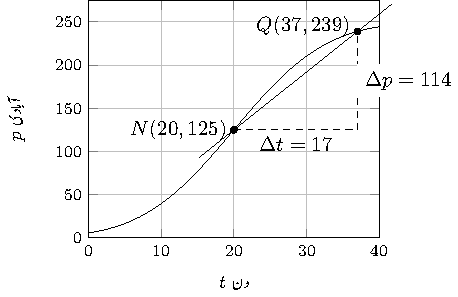
\includegraphics{normalDistributionFlies}
\caption{مکھی کی نمو آبادی}
\label{شکل_حد_مکھی_نمو_آبادی}
\end{minipage}\hfill
\begin{minipage}{0.45\textwidth}
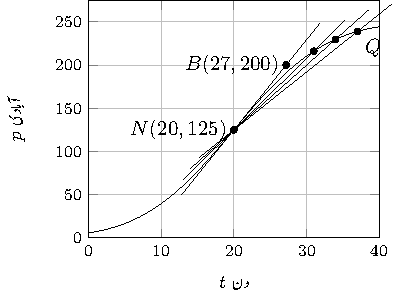
\includegraphics{normalDistributionFliesInstantaneous}
\caption{مکھی کی بیسویں دن نمو آبادی}
\label{شکل_حد_مکھی_نمو_آبادی_بیس}
\end{minipage}%
\end{figure}

حل:\quad
\عددی{20} ویں دن آبادی \عددی{125} تھی جبکہ \عددی{37} ویں دن آبادی \عددی{239} تھی۔ یوں \عددی{37-20=17} دنوں میں آبادی میں \عددی{239-125=114} تبدیل  رونما ہوئی۔یوں شرح تبدیلی درج ذیل ہو گی
\begin{align*}
\frac{\Delta p}{\Delta t}=\frac{114}{17}=6.7 (\text{\RL{مکھیاں فی دن}})
\end{align*}
جو شکل \حوالہ{شکل_حد_مکھی_نمو_آبادی} میں سیکنٹ \عددی{NQ} کی ڈھلوان ہے۔
\انتہا{مثال}
%========================

درج بالا مثال میں \عددی{20} ویں دن سے \عددی{37} ویں دن تک کی اوسط شرح تبدیلی حاصل کی گئی جو ہمیں \عددی{20} ویں دن کی تبدیلی کی شرح کے بارے میں کوئی معلومات فراہم نہیں کرتی ہے۔اس کے لئے ہمیں \عددی{20} ویں دن کے قریب حساب  کرنا ہو گا۔

\ابتدا{مثال}
مثال \حوالہ{مثال_حد_نمو_آبادی_مکھی} میں \عددی{20} ویں دن آبادی میں تبدیلی کی شرح کیا ہے؟\\
حل:\quad
ہمیں نقطہ \عددی{Q} کو نقطہ \عددی{N} کے قریب سے قریب تر کرتے ہوئے شرح حاصل کرنی ہو گی (شکل \حوالہ{شکل_حد_مکھی_نمو_آبادی_بیس})۔یوں درج ذیل حاصل ہوتا ہے۔
\begin{align*}
\begin{array}{ll}
Q&\frac{\Delta p}{\Delta t}\\
\hline
(37,239)&\frac{239-125}{37-20}=6.7\\
(35,230)&\frac{230-125}{35-20}=7\\
(32,216)&\frac{216-125}{32-20}=7.6\\
(27,200)&\frac{200-125}{27-20}=10.7
\end{array}
\end{align*}

جیسے جیسے \عددی{Q} کو بائیں منتقل کیا جائے، خط \عددی{NQ} نقطہ \عددی{N} کے گرد گھڑی کی الٹ رخ گھومتا ہے۔ہم دیکھتے ہیں کہ یہ خط آخر کار \عددی{NB} کو چھوتا ہے۔اس خط کو دیے گئے منحنی کا \اصطلاح{مماس}\فرہنگ{مماس}\حاشیہب{tangent}\فرہنگ{tangent} کہتے ہیں۔اس طرح ہم توقع کرتے ہیں کہ \عددی{20} ویں دن آبادی کی تبدیلی کی شرح \عددی{10.7} مکھیاں فی دن ہو گی۔
\انتہا{مثال}
%=======================

لمحہ \عددی{t=1} اور لمحہ \عددی{t=2} پر گرتے ہوئے پتھر کی رفتار یا \عددی{20} ویں دن شرح تبدیلی کو \اصطلاح{لمحاتی شرح تبدیلی}\فرہنگ{لمحاتی!شرح تبدیلی}\حاشیہب{instantaneous rates of change}\فرہنگ{instantaneous!rate of change} کہتے ہیں۔جیسا آپ نے دیکھا، ہم اوسط شرح تبدیلی کی تحدیدی قیمت سے لمحاتی شرح تبدیلی حاصل کرتے ہیں۔درج بالا مثال میں ہم نے خط مماس کو بطور خط سیکنٹ کی تحدیدی  صورت پیش کیا۔لمحاتی شرح اور مماس کا گہرا تعلق ہے جو دیگر موضوعات میں بھی پیش آتا ہے۔ اس تعلق کو مزید سمجھنے کی خاطر ہمیں  تحدیدی قیمتوں  کا تعین کرنا سیکھنا ہو گا جنہیں ہم \اصطلاح{حد}\فرہنگ{حد}\حاشیہب{limits}\فرہنگ{limits} کہتے ہیں۔ 

\جزوحصہء{تفاعل کی تحدیدی قیمتیں}
تحدیدی قیمت کی تعریف سے پہلی ایک اور مثال دیکھتے ہیں۔

\ابتدا{مثال}\شناخت{مثال_حد_عجیب_تفاعل_الف}
تفاعل \عددی{f(x)=\tfrac{x^2-1}{x-1}} نقطہ \عددی{x=1} کے قریب کیسا رویہ رکھتا ہے؟\\
حل:\quad
چونکہ صفر سے کسی بھی عدد کو تقسیم نہیں کیا جا سکتا ہے لہٰذا ماسوائے \عددی{x=1} کے، یہ کلیہ تمام حقیقی اعداد کے لئے \عددی{f} تعین کرتا ہے۔کسی بھی \عددی{x\ne 1} کے لئے ہم اس کلیہ کی سادہ صورت حاصل کر سکتے ہیں:
\begin{align*}
f(x)=\frac{x^2-1}{x-1}=\frac{(x-1)(x+1)}{x-1}=x+1\quad\quad (x\ne 1)
\end{align*} 
یوں خط \عددی{y=x+1} جس سے نقطہ \عددی{x=1} یعنی \عددی{(1,2)} خارج کیا گیا ہو اس تفاعل کو ظاہر کرتا ہے۔اس نقطہ کو شکل \حوالہ{شکل_مثال_حد_عجیب_تفاعل_الف} میں بطور سوراخ دکھایا گیا ہے۔اگرچہ نقطہ \عددی{f(1)} غیر معین ہے، ہم \عددی{ x} کی قیمت \عددی{1} کے قریب سے قریب لیتے ہوئے \عددی{f(x)} کی قیمت \عددی{2} کے جتنی قریب چاہیں کر سکتے ہیں۔
\begin{figure}
\centering
\begin{tikzpicture}
\draw[-latex](-1.5,0)--(3,0)node[right]{$x$};
\draw[-latex](0,-0.2)--(0,2.5)node[above]{$y$};
\draw[shorten <=-0.5cm,shorten >=-0.5cm](-1,0)--(1,2);
\foreach \x in {-1,1}{\draw(\x,0)node[below]{$\x$}--++(0,0.1);}
\foreach \y in {1,2}{\draw(0,\y)node[left]{$\y$}--++(0.1,0);}
\draw(1,2)node[ocirc]{};
\draw(0.5,1)node[right]{$y=f(x)=\tfrac{x^2-1}{x-1}$};
\end{tikzpicture}
\caption{شکل برائے مثال \حوالہ{مثال_حد_عجیب_تفاعل_الف}}
\label{شکل_مثال_حد_عجیب_تفاعل_الف}
\end{figure}
%
\begin{align*}
\begin{array}{ll}
\multicolumn{1}{c}{x (\ne 1)}&\multicolumn{1}{c}{f(x)=\tfrac{x^2-1}{x-1}=x+1,\,\, (x\ne 1)}\\
\hline
0.9&1.9\\
1.1&2.1\\
0.99&1.99\\
1.01&2.01\\
0.999&1.999\\
1.001&2.001\\
0.999999&1.999999\\
1.000001&2.000001
\end{array}
\end{align*}

ہم کہتے ہیں کہ \عددی{x} کی قیمت \عددی{1} تک پہنچنے سے \عددی{f(x)} کی قیمت \عددی{2} تک پہنچتی ہے یا \عددی{x} ایک تک پہنچنے سے \عددی{f(x)} تحدیدی قیمت \عددی{2} تک پہنچتی ہے یا حد \عددی{2} تک پہنچتی ہے، جس کو درج ذیل لکھا جاتا ہے۔
\begin{align*}
\lim_{x\to 1} f(x)=2 \quad \text{یا}\quad \lim_{x\to 1} \frac{x^2-1}{x-1}=2
\end{align*}
\عددی{x} کی قیمت \عددی{x_0} تک پہنچنے کو \عددی{x\to x_0} لکھا جاتا ہے۔
\انتہا{مثال}
%====================== 

\ابتدا{تعریف}\موٹا{حد کی غیر رسمی تعریف}\\
فرض کریں کہ \عددی{x_0} کی پڑوس میں ایک کھلے وقفہ پر تفاعل \عددی{f(x)} معین ہے۔یہ تفاعل نقطہ \عددی{x_0} پر غیر معین ہو سکتا ہے۔ اگر \عددی{x_0} کے کافی قریب \عددی{x} کی  تمام قیمتوں کے لئے \عددی{f(x)} کی قیمتیں \عددی{L} کے کافی قریب پائی جاتی ہوں تب ہم کہتے ہیں کہ \عددی{x} کی قیمت \عددی{x_0} تک پہنچنے سے \عددی{f} کی قیمت \اصطلاح{حد} \عددی{L} تک پہنچتی ہے۔ اس کو ہم درج ذیل لکھتے ہیں۔
\begin{align*}
\lim_{x\to x_0} f(x)=L
\end{align*}
\انتہا{تعریف}
%========================

اس تعریف کو غیر رسمی اس لئے کہا گیا ہے کہ "کافی قریب" کی طرز کے فقرے بہت ٹھیک نہیں ہیں۔خراد پر کام کرنے والے ماہر کے لئے کافی قریب سے مراد \عددی{\SI{10}{\micro\meter}} ہو سکتا ہے جبکہ ماہر فلکیات کے لئے اس کا مطلب چند ہزار نوری سال ہو سکتا ہے۔البتہ یہ تعریف اتنی درست ضرور ہے کہ ہم حد کو پہچان سکیں اور اس کی قیمت حاصل کر سکیں۔ہم حد کی بالکل ٹھیک تعریف جلد پیش کریں گے۔

\ابتدا{مثال}\شناخت{مثال_حد_عجیب_تفاعل_ب}
\عددی{x\to x_0} کی صورت میں \عددی{f} کی حد کی وجودیت \عددی{x_0} پر \عددی{f} کی تعریف کے تابع نہیں ہے۔ شکل \حوالہ{شکل_مثال_حد_عجیب_تفاعل_ب} میں  \عددی{f} کا \عددی{x\to 1} پر حد \عددی{2} ہے اگرچہ \عددی{x=1} پر \عددی{f} غیر معین ہے۔تفاعل \عددی{g} کا \عددی{x\to 1} پر حد \عددی{2} ہے اگرچہ \عددی{x=1} پر \عددی{g(1)=1} ہے۔یوں \عددی{\lim\limits_{x\to 1}g(x)\ne g(1)} ہو گا۔صرف تفاعل \عددی{h} کا \عددی{x\to 1} پر حد اور قیمت دونوں \عددی{2} کے برابر ہیں یعنی \عددی{\lim\limits_{x\to 1} h(x)=h(1)}۔
\begin{figure}
\centering
\begin{subfigure}{0.33\textwidth}
\centering
\begin{tikzpicture}[x=0.75cm]
\draw[-latex](-1.5,0)--(2,0)node[right]{$x$};
\draw[-latex](0,-0.2)--(0,2.5)node[above]{$y$};
\draw[shorten <=-0.5cm,shorten >=-0.5cm](-1,0)--(1,2);
\foreach \x in {-1,1}{\draw(\x,0)node[below]{$\x$}--++(0,0.1);}
\foreach \y in {1,2}{\draw(0,\y)node[left]{$\y$}--++(0.1,0);}
\draw(1,2)node[ocirc]{};
\draw(0,-1)node[font=\footnotesize]{$\begin{aligned}f(x)=\tfrac{x^2-1}{x-1}\end{aligned}$};
\end{tikzpicture}
\caption{}
\end{subfigure}%
\begin{subfigure}{0.33\textwidth}
\centering
\begin{tikzpicture}[x=0.75cm]
\draw[-latex](-1.5,0)--(2,0)node[right]{$x$};
\draw[-latex](0,-0.2)--(0,2.5)node[above]{$y$};
\draw[shorten <=-0.5cm,shorten >=-0.5cm](-1,0)--(1,2);
\foreach \x in {-1,1}{\draw(\x,0)node[below]{$\x$}--++(0,0.1);}
\foreach \y in {1,2}{\draw(0,\y)node[left]{$\y$}--++(0.1,0);}
\draw(1,2)node[ocirc]{};
\draw(1,1)node[circ]{};
\draw(0,-1)node[font=\footnotesize]{$\begin{aligned}g(x)=\begin{cases}\tfrac{x^2-1}{x-1},&x\ne 1\\ 1,&x=1\end{cases}\end{aligned}$};
\end{tikzpicture}
\caption{}
\end{subfigure}%
\begin{subfigure}{0.33\textwidth}
\centering
\begin{tikzpicture}[x=0.75cm]
\draw[-latex](-1.5,0)--(2,0)node[right]{$x$};
\draw[-latex](0,-0.2)--(0,2.5)node[above]{$y$};
\draw[shorten <=-0.5cm,shorten >=-0.5cm](-1,0)--(1,2);
\foreach \x in {-1,1}{\draw(\x,0)node[below]{$\x$}--++(0,0.1);}
\foreach \y in {1,2}{\draw(0,\y)node[left]{$\y$}--++(0.1,0);}
\draw(1,2)node[circ]{};
\draw(0,-1)node[font=\footnotesize]{$\begin{aligned}h(x)=x+1\end{aligned}$};
\end{tikzpicture}
\caption{}
\end{subfigure}%
\caption{$\lim\limits_{x\to 1} f(x)=\lim\limits_{x\to 1}g(x)=\lim\limits_{x\to 1} h(x)=2\quad $}
\label{شکل_مثال_حد_عجیب_تفاعل_ب}
\end{figure}
\انتہا{مثال}
%============================

بعض اوقات \عددی{\lim\limits_{x\to x_0}f(x)} کی قیمت \عددی{f(x_0)} سے حاصل کی جا سکتی ہے۔اس کی مثال تفاعل \عددی{f(x)} ہے جو کثیر رکنی اور تکونیاتی تفاعل کا الجبرائی مجموعہ  ہے اور جہاں \عددی{x_0} پر \عددی{f(x_0)} معین ہو۔

%===============================
\ابتدا{مثال}\شناخت{مثال_حد_عجیب_تفاعل_پ}
\begin{enumerate}[a.]
\item
$\lim\limits_{x\to 2} (4)=4$
\item
$\lim\limits_{x\to 13}(4)=4$
\item
$\lim\limits_{x\to 3} x=3$
\item
$\lim\limits_{x\to 2} (5x-3)=10-3=7$
\item
$\lim\limits_{x\to -2}\frac{3x+4}{x+5}=\frac{-6+4}{-2+5}=-\frac{2}{3}$
\end{enumerate}
\انتہا{مثال}
%================================
\ابتدا{مثال}\شناخت{مثال_حد_مماثل_تفاعل}
\begin{enumerate}[a.]
\item
اگر \عددی{f} مماثلی تفاعل \عددی{f(x)=x} ہو تب \عددی{x_0} کے کسی بھی قیمت کے لئے  درج ذیل ہو گا (شکل \حوالہ{شکل_مثال_حد_عجیب_تفاعل_پ}-ل)۔
\begin{align*}
\lim\limits_{x\to x_0} f(x)=\lim\limits_{x\to x_0} x=x_0
\end{align*}
\item
اگر \عددی{f} مستقل تفاعل \عددی{f(x)=k} ہو (جہاں \عددی{k} مستقل ہے) تب \عددی{x_0} کے کسی بھی قیمت کے لئے درج ذیل ہو گا (شکل \حوالہ{شکل_مثال_حد_عجیب_تفاعل_پ}-ب)۔
\begin{align*}
\lim\limits_{x\to x_0} f(x)=\lim\limits_{x\to x_0} k=k
\end{align*} 
\end{enumerate}
%
\begin{figure}
\centering
\begin{subfigure}{0.5\textwidth}
\centering
\begin{tikzpicture}
\draw[-latex](-0.25,0)--(3,0)node[right]{$x$};
\draw[-latex](0,-0.2)--(0,2)node[above]{$y$};
\draw[shorten <=-0.5cm](0,0)--(2,2)node[pos=1,left]{$y=x$};
\draw[dashed] (0,1)node[left]{$x_0$}--(1,1)--(1,0)node[below]{$x_0$};
\end{tikzpicture}
\caption{مماثل تفاعل}
\end{subfigure}%
\begin{subfigure}{0.5\textwidth}
\centering
\begin{tikzpicture}
\draw[-latex](-0.25,0)--(3,0)node[right]{$x$};
\draw[-latex](0,-0.2)--(0,2)node[above]{$y$};
\draw(-0.25,1)--(3,1)node[pos=0.9,above]{$y=k$};
\draw(0,1)node[circ]{}node[above left]{$k$};
\draw[dashed](1,0)node[below]{$x_0$}--(1,1)node[circ]{};
\draw(0,0)node[below left]{$M$};
\end{tikzpicture}
\caption{مستقل تفاعل}
\end{subfigure}%
\caption{اشکال برائے مثال \حوالہ{مثال_حد_عجیب_تفاعل_پ}}
\label{شکل_مثال_حد_عجیب_تفاعل_پ}
\end{figure}
\انتہا{مثال}
%==================================
\ابتدا{مثال}\شناخت{مثال_حد_عجیب_تفاعل_ت} \ترچھا{عین ممکن ہے کہ تفاعل کے دائرہ کار میں تفاعل کا حد نہ پایا جاتا ہو۔}\\ 
درج ذیل تفاعل کا \عددی{x\to 0} پر رویہ کیسا ہو گا؟
\begin{enumerate}[a.]
\item
$U(x)=\begin{cases}0,&x<0\\ 1,&x\ge 0  \end{cases}$
\item
$g(x)=\begin{cases} \tfrac{1}{x},&x\ne 0\\ 0,&x=0 \end{cases}$
\item
$f(x)=\begin{cases}0,&x\le 0\\ \sin \tfrac{1}{x},&x>0  \end{cases}$
\end{enumerate}
%

حل:\quad
\begin{enumerate}[a.]
\item
اکائی سیڑھی تفاعل \عددی{U(x)} کا \عددی{x\to 0} پر کوئی حد نہیں پایا جاتا ہے چونکہ اس نقطہ پر تفاعل کی چھلانگ پائی جاتی ہے۔\عددی{0} کے کافی قریب \عددی{x} کی منفی قیمتوں کے لئے \عددی{U} کی قیمت \عددی{0} ہے جبکہ \عددی{0} کے کافی  قریب  \عددی{x}  کی مثبت قیمتوں کے لئے \عددی{U} کی قیمت \عددی{1} ہے۔یوں \عددی{0} کے قریب پہنچنے سے \عددی{U} کی منفرد قیمت نہیں پائی جاتی ہے (شکل \حوالہ{شکل_مثال_حد_عجیب_تفاعل_ت}-ا)۔
\item
\عددی{x=0} کے کافی قریب تفاعل کی قیمت بے قابو بڑھتی ہے اور کسی ایک منفرد قیمت تک پہنچنے کی کوشش نہیں کرتی ہے (شکل \حوالہ{شکل_مثال_حد_عجیب_تفاعل_ت}-ب)۔
\item
\عددی{x=0} کے کافی قریب تفاعل بہت زیادہ ارتعاش کرتا ہے۔اس کی قیمت کسی مخصوص قیمت تک پہنچنے کی کوشش نہیں کرتی ہے (شکل \حوالہ{شکل_مثال_حد_عجیب_تفاعل_ت}-ج)۔ 
\end{enumerate}
%
\begin{figure}
\centering
\begin{subfigure}{0.33\textwidth}
\centering
\begin{tikzpicture}
\begin{axis}[clip=false,small,axis lines=middle,width=4cm,xtick={\empty},ytick={1},xlabel={$x$},ylabel={$y$},xlabel style={at={(current axis.right of origin)},anchor={west}},ylabel style={at={(current axis.above origin)},anchor=south},ymin=-0.5,ymax=2]
\addplot[domain=-2:0]{0};
\addplot[domain=0:2]{1};
\draw(axis cs:0,0)node[ocirc]{};
\draw(axis cs:0,1)node[circ]{};
\draw(axis cs:0,1)node[above right,font=\footnotesize]{$\begin{aligned}y=\begin{cases}0,&x<0\\ 1,&x\ge 1\end{cases}\end{aligned}$};
\end{axis}
\end{tikzpicture}
\caption{اکائی سیڑھی تفاعل $U(x)\,\,$}
\end{subfigure}%
\begin{subfigure}{0.33\textwidth}
\centering
\begin{tikzpicture}
\begin{axis}[clip=false,small,axis lines=middle,width=4cm,xtick={\empty},ytick={\empty},xlabel={$x$},ylabel={$y$},xlabel style={at={(current axis.right of origin)},anchor={west}},ylabel style={at={(current axis.above origin)},anchor=south}]
\addplot[domain=-4:-0.3]{1/x};
\addplot[domain=0.3:4]{1/x};
\draw(axis cs:0,0)node[circ]{}node[below right]{$0$};
\draw(axis cs:0.4,1)node[above right,font=\footnotesize]{$\begin{aligned}y=\begin{cases}\tfrac{1}{x},&x\ne 0\\ 0,&x=0\end{cases}\end{aligned}$};
\end{axis}
\end{tikzpicture}
\caption{$g(x)$}
\end{subfigure}%
\begin{subfigure}{0.33\textwidth}
\centering
\begin{tikzpicture}
\begin{axis}[clip=false,small,axis lines=middle,width=4cm,xtick={\empty},ytick={-1,1},xlabel={$x$},ylabel={$y$},xlabel style={at={(current axis.right of origin)},anchor={west}},ylabel style={at={(current axis.above origin)},anchor=south},ymin=-1.2,ymax=1.2]
\addplot[domain=-0.2:0]{0}node[circ]{};
\addplot[domain=0.052:0.08,samples=100]{sin(180/(pi*x)};
\addplot[domain=0.08:0.5,samples=100]{sin(180/(pi*x)};
\draw(axis cs:0,0)node[circ]{}node[below left]{$0$};
\draw(axis cs:0.2,-0.75)node[right,font=\footnotesize]{$\begin{aligned}y=\begin{cases}0 ,&x\le  0\\  \sin \tfrac{1}{x},&x>0\end{cases}\end{aligned}$};
\end{axis}
\end{tikzpicture}
\caption{$f(x)$}
\end{subfigure}%
\caption{اشکال برائے مثال \حوالہ{مثال_حد_عجیب_تفاعل_ت}}
\label{شکل_مثال_حد_عجیب_تفاعل_ت}
\end{figure}
\انتہا{مثال}
%=================================

\حصہء{سوالات \حوالہ{حصہ_حد_تبدیلی_کی_شرح_اور_حد}}

\موٹا{ترسیم سے حد}

\ابتدا{سوال}\شناخت{سوال_حد_ترسیم_سے_حد_الف}
شکل \حوالہ{شکل_سوال_حد_ترسیم_سے_حد_الف}-ا میں دی گئی ترسیم سے درج ذیل حد تلاش کریں یا حد نا ہونے کی وجہ بیان کریں۔
\begin{multicols}{3}
\begin{enumerate}[a.]
\item
$\lim\limits_{x\to 1} g(x)$
\item
$\lim\limits_{x\to 2} g(x)$
\item
$\lim\limits_{x\to 3}g(x)$
\end{enumerate}
\end{multicols}
%
\begin{figure}
\centering
\begin{subfigure}{0.5\textwidth}
\centering
\begin{tikzpicture}
\draw[-latex](-0.25,0)--(4,0)node[right]{$x$};
\draw[-latex](0,-0.2)--(0,1.5)node[above]{$y$};
\draw[dashed](0,1)node[left]{$1$}--(3,1)node[solid,circ]{};
\draw(-0.2,-0.2)--(1,1)node[ocirc]{};
\draw(1,0)node[circ]{}--(2,1)node[circ]{}node[above,yshift={2mm}]{$y=g(x)$}--(3,0)node[ocirc]{}--(3.9,0.9);
\foreach \x in {1,2,3}{\draw(\x,0)node[below]{$\x$}--++(0,0.1);}
\end{tikzpicture}
\caption{}
\end{subfigure}%
\begin{subfigure}{0.5\textwidth}
\centering
\begin{tikzpicture}
\draw[-latex](-3,0)--(2,0)node[right]{$t$};
\draw[-latex](0,-1.25)--(0,1.5)node[above]{$s$};
\draw(-3,-1)--(-2,0)node[ocirc]{}node[above,yshift={2mm}]{$s=f(t)$}--(-1,-1)node[circ]{}--(0,-1)node[ocirc]{}node[right]{$-1$};
\foreach \x in {-2,-1,1}{\draw(\x,0)node[below]{$\x$}--++(0,0.1);}
\draw(0,0)node[circ]{}node[below left]{$0$};
\draw(0,1)node[ocirc]{}node[left]{$1$}--(2,1);
\end{tikzpicture}
\caption{}
\end{subfigure}%
\caption{اشکال برائے سوال \حوالہ{سوال_حد_ترسیم_سے_حد_الف} اور سوال \حوالہ{سوال_حد_ترسیم_سے_حد_ب}}
\label{شکل_سوال_حد_ترسیم_سے_حد_الف}
\end{figure}
\انتہا{سوال}
%=====================
\ابتدا{سوال}\شناخت{سوال_حد_ترسیم_سے_حد_ب}
شکل \حوالہ{شکل_سوال_حد_ترسیم_سے_حد_الف}-ب میں دی گئی ترسیم سے درج ذیل حد تلاش کریں یا حد نا ہونے کی وجہ بیان کریں۔
\begin{multicols}{3}
\begin{enumerate}[a.]
\item
$\lim\limits_{t\to -2}f(t)$
\item
$\lim\limits_{t\to -1}f(t)$
\item
$\lim\limits_{t\to 0}f(t)$
\end{enumerate}
\end{multicols}
\انتہا{سوال}
%======================
\ابتدا{سوال}\شناخت{سوال_حد_ترسیم_سے_حد_پ}
تفاعل \عددی{y=f(x)}  (شکل \حوالہ{سوال_حد_ترسیم_سے_حد_پ}-ا) کے لئے درج ذیل فقروں میں سے کون سے درست ہیں؟
\begin{multicols}{3}
\begin{enumerate}[a.]
\item
$\lim\limits_{x\to 0}f(x)$ موجود ہے\\
\item
$\lim\limits_{x\to 0}f(x)=0$
\item
$\lim\limits_{x\to 0}f(x)=1$
\item
$\lim\limits_{x\to 1}f(x)=1$
\item
$\lim\limits_{x\to 1}f(x)=0$
\item
$\lim\limits_{x\to x_ 0}f(x)$
وقفہ \عددی{(-1,1)} میں ہر نقطہ \عددی{x_0} پر موجود ہے
\end{enumerate}
\end{multicols}
%
\begin{figure}
\centering
\begin{subfigure}{0.5\textwidth}
\centering
\begin{tikzpicture}
\draw[-latex](-1.2,0)--(3,0)node[right]{$x$};
\draw[-latex](0,-1.2)--(0,1.5)node[above]{$y$};
\draw(-1,-1)node[circ]{}--(0,0)node[ocirc]{}--(1,-1)node[ocirc]{} (1,0)node[circ]{}--(2,1)node[circ]{};
\draw(0,1)node[circ]{}node[left]{$1$}--++(0.1,0);
\foreach \x in {-1,1,2}{\draw(\x,0)node[below]{$\x$}--++(0,0.1);} 
\draw(0,-1)node[left]{$-1$}--++(0.1,0);
\draw(0.5,1.25)node[right]{$y=f(x)$};
\end{tikzpicture}
\caption{}
\end{subfigure}%
\begin{subfigure}{0.5\textwidth}
\centering
\begin{tikzpicture}[]
\draw[-latex](-1.2,0)--(3.5,0)node[right]{$x$};
\draw[-latex](0,-2.2)--(0,1.5)node[above]{$y$};
\foreach \x in {-1,1,2,3}{\draw(\x,0)node[below]{$\x$}--++(0,0.1);} 
\foreach \y in {-2,-1,1}{\draw(0,\y)node[left]{$\y$}--++(0.1,0);}
\draw(-1,-1)node[circ]{}--(0,0)node[circ]{};
\draw[domain=0:1] plot ({\x},{-2*\x*\x});
\draw([shift={(0:1)}]2,0) arc (0:180:1);
\draw(1,0)node[circ]{} (2,0)node[circ]{} (3,0)node[circ]{} (2,1)node[ocirc]{}node[above]{$y=f(x)$};
\end{tikzpicture}
\caption{}
\end{subfigure}%
\caption{اشکال برائے سوال \حوالہ{سوال_حد_ترسیم_سے_حد_پ} اور سوال \حوالہ{سوال_حد_ترسیم_سے_حد_ت}}
\label{شکل_سوال_حد_ترسیم_سے_حد_پ}
\end{figure}
\انتہا{سوال}
%============================
\ابتدا{سوال}\شناخت{سوال_حد_ترسیم_سے_حد_ت}
تفاعل \عددی{y=f(x)} (شکل \حوالہ{سوال_حد_ترسیم_سے_حد_پ}-ب)  کے لئے درج ذیل فقروں میں سے کون سے درست ہیں؟
\begin{multicols}{3}
\begin{enumerate}[a.]
\item
$\lim\limits_{x\to 2} f(x)$
موجود نہیں ہے
\item
$\lim\limits_{x\to 2}f(x)=2$
\item
$\lim\limits_{x\to 1}f(x)$
موجود نہیں ہے
\item
$\lim\limits_{x\to x_0}f(x)$
وقفہ \عددی{(-1,1)} میں ہر نقطہ \عددی{x_0} پر موجود ہے۔
\item
$\lim\limits_{x\to x_0}f(x)$
وقفہ \عددی{(1,3)} میں ہر نقطہ \عددی{x_0} پر موجود ہے۔
\end{enumerate}
\end{multicols}
\انتہا{سوال}
%======================

\موٹا{وجودیت اور حد}

سوال \حوالہ{سوال_حد_غیر_موجود_الف} اور سوال \حوالہ{سوال_حد_غیر_موجود_ب} میں حد کی غیر موجودگی کی وجہ بیان کریں۔

\ابتدا{سوال}\شناخت{سوال_حد_غیر_موجود_الف}
$\lim\limits_{x \to 0}\tfrac{x}{\abs{x}}$
\انتہا{سوال}
%======================
\ابتدا{سوال}\شناخت{سوال_حد_غیر_موجود_ب}
$\lim\limits_{x \to 1}\tfrac{1}{x-1}$
\انتہا{سوال}
%======================
\ابتدا{سوال}
فرض کریں کہ ماسوائے نقطہ \عددی{x=x_0} تفاعل \عددی{f(x)} تمام حقیقی \عددی{x} کے لئے معین ہے۔کیا \عددی{\lim\limits_{x\to x_0}f(x)} کی وجودیت کی وجودیت کے بارے میں کچھ کہنا ممکن ہے؟ اپنے جواب کی وجہ بیان کریں۔ 
\انتہا{سوال}
%======================
\ابتدا{سوال}
فرض کریں کہ  تفاعل \عددی{f(x)} وقفہ \عددی{[-1,1]} میں تمام  \عددی{x} کے لئے معین ہے۔کیا \عددی{\lim\limits_{x\to 0}f(x)} کے بارے میں کچھ کہنا ممکن ہے؟ اپنے جواب کی وجہ بیان کریں۔ 
\انتہا{سوال}
%======================
\ابتدا{سوال}
اگر \عددی{\lim\limits_{x\to 1}f(x)=5} ہو تب کیا \عددی{x=1} پر \عددی{f} کا معین ہونا لازم ہے؟اگر معین ہونا لازم ہو تب کیا \عددی{f(1)=5} ہونا لازم ہے؟ کیا \عددی{x=1} پر ہم \عددی{f} کی قیمت کے بارے میں کچھ کہہ سکتے ہیں؟ وضاحت کریں۔
\انتہا{سوال}
%======================
\ابتدا{سوال}
اگر \عددی{f(1)=5} ہو تب کیا \عددی{\lim\limits_{x\to 1}f(x)} لازماً موجود ہو گا؟ اگر ایسا ہو تب کیا \عددی{\lim\limits_{x\to 1}f(x)=5} لازماً ہو گا؟ کیا ہم  \عددی{\lim\limits_{x\to 1}f(x)} کے بارے میں کوئی نتیجہ اخذ کر سکتے ہیں؟ وضاحت کریں۔
\انتہا{سوال}
%======================

\موٹا{کیلکولیٹر اور کمپیوٹر کا استعمال}

\ابتدا{سوال}
\عددی{f(x)=\tfrac{x^2-9}{x+3}} لیں۔
\begin{enumerate}[a.]
\item
\عددی{f} کی قیمتوں کا جدول نقاط \عددی{x=-3.1,-3.01,-3.001,\cdots} پر وہاں تک تلاش کریں جہاں تک آپ کا کیلکولیٹر جواب حاصل کر سکتا ہو۔اس جدول سے \عددی{\lim\limits_{x\to -3}f(x)} کی اندازاً قیمت حاصل کریں۔اس کے برعکس نقاط \عددی{x=-2.9,-2.99,\cdots} پر \عددی{f} کی قیمتیں استعمال کرتے ہوئے نتیجہ کیا ہو گا؟
\item
تفاعل کو \عددی{x_0=-3} کے قریب ترسیم کریں۔ ترسیم پر \عددی{x\to -3} کے لئے \عددی{y} کی قیمت دیکھ کر  گزشتہ جزو کے نتائج کی تصدیق کریں۔ 
\item
\عددی{\lim\limits_{x\to -3}f(x)} کو الجبرائی طریقہ سے اخذ کریں۔
\end{enumerate}
\انتہا{سوال}
%=========================
\ابتدا{سوال}
\عددی{g(x)=\tfrac{x^2-2}{x-\sqrt{2}}} لیں۔
\begin{enumerate}[a.]
\item
\عددی{\sqrt{2}} کی تخمینی قیمتوں \عددی{x=1.4,1.41,1.414,\cdots} پر تفاعل کی قیمتوں کے جدول سے \عددی{\lim\limits_{x\to \sqrt{2}}g(x)}  کی اندازاً قیمت حاصل کریں۔
\item
نقطہ \عددی{x_0=\sqrt{2}} کے قریب تفاعل ترسیم کریں۔\عددی{x\to \sqrt{2}} کے لئے ترسیم سے \عددی{y} کی قیمت دیکھ کر گزشتہ جزو کی جواب کا تصدیق کریں۔
\item
\عددی{\lim\limits_{x\to\sqrt{2}}g(x)} کو الجبرائی طور پر حاصل کریں۔
\end{enumerate}
\انتہا{سوال}
%====================
\ابتدا{سوال}
\عددی{G(x)=\tfrac{x+6}{x^2+4x-12}} لیں۔
\begin{enumerate}[a.]
\item
نقاط \عددی{x=-5.9,-5.99,-5.999,\cdots} پر \عددی{G} کی قیمتوں کا جدول بنا کر \عددی{\lim\limits_{x\to -6}G(x)} کی اندازاً قیمت حاصل کریں۔ اس کے برعکس \عددی{x=-6.1,-6.01,-6.001,\cdots} پر \عددی{G} کی قیمتیں استعمال کرتے ہوئے کیا نتیجہ حاصل ہو گا؟
\item
\عددی{G} کو \عددی{x_0=6} کے قریبی نقطوں پر تقسیم کرتے ہوئے \عددی{x\to -6} کے لئے \عددی{G} کی قیمت دیکھ کر گزشتہ جزو کے نتائج کی تصدیق کریں۔
\item
\عددی{\lim\limits_{x\to -6}G(x)} کو الجبرائی طریقہ سے حاصل کریں۔
\end{enumerate}
\انتہا{سوال}
%======================
\ابتدا{سوال}
\عددی{h(x)=\tfrac{x^2-2x-3}{x^2-4x+3}} لیں۔
\begin{enumerate}[a.]
\item
نقاط \عددی{x=2.9, 2.99, 2.999,\cdots} پر \عددی{h} کی قیمتوں کے جدول سے \عددی{\lim\limits_{x\to 3}h(x)} کی اندازاً قیمت تلاش کریں۔اس کے برعکس \عددی{x=3.1,3.01,3.001,\cdots} پر \عددی{h} کی قیمتیں لیتے ہوئے نتیجہ کیا ہو گا؟
\item
\عددی{x_0=3} کے قریب \عددی{h} ترسیم کر کے \عددی{x\to 3} کے لئے \عددی{h(x)} کی قیمت دیکھ کر گزشتہ جزو کے نتائج کی تصدیق کریں۔
\item
\عددی{\lim\limits_{x\to 3}h(x)} کو الجبرائی طریقہ سے حاصل کریں۔
\end{enumerate}
\انتہا{سوال}
%=====================
\ابتدا{سوال}
\عددی{f(x)=\tfrac{x^2-1}{\abs{x}-1}} لیں۔
\begin{enumerate}[a.]
\item
\عددی{f} کی قیمتوں کا جدول \عددی{x} کی ان قیمتوں کے لئے بنائیں جو \عددی{x_0=-1} تک نیچے سے اور اوپر سے پہنچنے کی کوشش کرتی ہیں۔اس جدول سے \عددی{\lim\limits_{x\to-1}f(x)} کی اندازاً قیمت تلاش کریں۔  
\item
\عددی{x_0=-1} کے قریب \عددی{f} ترسیم کریں۔ترسیم سے \عددی{x\to -1} کے لئے \عددی{y} کی قیمتیں دیکھ کر گزشتہ جزو کے نتائج کی تصدیق کریں۔
\item
\عددی{\lim\limits_{x\to -1}f(x)} کو الجبرائی طریقہ سے حاصل کریں۔
\end{enumerate}
\انتہا{سوال}
%========================
\ابتدا{سوال}
\عددی{F(x)=\tfrac{x^2+3x+2}{2-\abs{x}}} لیں۔
\begin{enumerate}[a.]
\item
\عددی{F} کی قیمتوں کا جدول \عددی{x} کی ان قیمتوں کے لئے بنائیں جو \عددی{x_0=-2} تک نیچے سے اور اوپر سے پہنچنے کی کوشش کرتی ہیں۔اس جدول سے
 \عددی{\lim\limits_{x\to-2}F(x)} کی اندازاً قیمت تلاش کریں۔  
\item
\عددی{x_0=-2} کے قریب \عددی{F} ترسیم کریں۔ترسیم سے \عددی{x\to -2} کے لئے \عددی{y} کی قیمتیں دیکھ کر گزشتہ جزو کے نتائج کی تصدیق کریں۔
\item
\عددی{\lim\limits_{x\to -2}F(x)} کو الجبرائی طریقہ سے حاصل کریں۔
\end{enumerate}
\انتہا{سوال}
%========================
\ابتدا{سوال}
\عددی{g(\theta)=\tfrac{\sin\theta}{\theta}} لیں۔
\begin{enumerate}[a.]
\item
\عددی{g} کی قیمتوں کا جدول \عددی{\theta} کی ان قیمتوں کے لئے بنائیں جو \عددی{\theta_0=0} تک نیچے سے اور اوپر سے پہنچنے کی کوشش کرتی ہیں۔اس جدول سے
 \عددی{\lim\limits_{x\to 0}g(\theta)} کی اندازاً قیمت تلاش کریں۔  
\item
\عددی{\theta_0=0} کے قریب \عددی{g} ترسیم کریں۔ترسیم سے گزشتہ جزو کے نتائج کی تصدیق کریں۔
\end{enumerate}
\انتہا{سوال}
%========================
\ابتدا{سوال}
\عددی{G(t)=\tfrac{1-\cos t}{t^2}} لیں۔
\begin{enumerate}[a.]
\item
\عددی{G} کی قیمتوں کا جدول \عددی{t} کی ان قیمتوں کے لئے بنائیں جو \عددی{t_0=0} تک نیچے سے اور اوپر سے پہنچنے کی کوشش کرتی ہیں۔اس جدول سے
 \عددی{\lim\limits_{t\to 0}G(t)} کی اندازاً قیمت تلاش کریں۔  
\item
\عددی{t_0=0} کے قریب \عددی{G} ترسیم کریں۔ترسیم سے گزشتہ جزو کے نتائج کی تصدیق کریں۔
\end{enumerate}
\انتہا{سوال}
%===================
\ابتدا{سوال}
\عددی{f(x)=x^{\tfrac{1}{1-x}}} لیں۔
\begin{enumerate}[a.]
\item
\عددی{f} کی قیمتوں کا جدول \عددی{x} کی ان قیمتوں کے لئے بنائیں جو \عددی{x_0=1} تک نیچے سے اور اوپر سے پہنچنے کی کوشش کرتی ہیں۔کیا \عددی{x} کی قیمت \عددی{x\to 1} تک پہنچنے سے \عددی{f} کا تحدیدی نقطہ پایا جاتا ہے؟ اگر تحدیدی نقطہ پایا جاتا ہو، اس کا تلاش کریں۔اگر نہیں پایا جاتا ہو تب وجہ بیان کریں۔
\item
\عددی{x_0=1} کے قریب \عددی{f} ترسیم کریں۔ترسیم سے گزشتہ جزو کے نتائج کی تصدیق کریں۔
\end{enumerate}
\انتہا{سوال}
%=============================
\ابتدا{سوال}
\عددی{f(x)=\tfrac{3^x-1}{x}} لیں۔
\begin{enumerate}[a.]
\item
\عددی{f} کی قیمتوں کا جدول \عددی{x} کی ان قیمتوں کے لئے بنائیں جو \عددی{x_0=0} تک نیچے سے اور اوپر سے پہنچنے کی کوشش کرتی ہیں۔کیا
 \عددی{x} کی قیمت \عددی{x\to 0} تک پہنچنے سے \عددی{f} کا تحدیدی نقطہ پایا جاتا ہے؟ اگر تحدیدی نقطہ پایا جاتا ہو، اس کا تلاش کریں۔اگر نہیں پایا جاتا ہو تب وجہ بیان کریں۔
\item
\عددی{x_0=0} کے قریب \عددی{f} ترسیم کریں۔ترسیم سے گزشتہ جزو کے نتائج کی تصدیق کریں۔
\end{enumerate}
\انتہا{سوال}
%=============================
\موٹا{متغیر کی تحدیدی قیمت پر کرتے ہوئے حد کا تعین}

سوال \حوالہ{سوال_حد_پر_الف} تا سوال \حوالہ{سوال_حد_پر_ب} میں متغیر \عددی{x} کی تحدیدی قیمت کو تفاعل میں پر کرتے ہوئے تفاعل کی حد تلاش کریں۔

\ابتدا{سوال}\شناخت{سوال_حد_پر_الف}
$\lim\limits_{x\to 2} 2x$
\انتہا{سوال}
%========================
\ابتدا{سوال}
$\lim\limits_{x\to 0} 2x$
\انتہا{سوال}
%========================
\ابتدا{سوال}
$\lim\limits_{x\to \tfrac{1}{3}} (3x-1)$
\انتہا{سوال}
%========================
\ابتدا{سوال}
$\lim\limits_{x\to 1} -\tfrac{1}{3x-1}$
\انتہا{سوال}
%========================
\ابتدا{سوال}
$\lim\limits_{x\to -1} 3x(2x-1)$
\انتہا{سوال}
%========================
\ابتدا{سوال}
$\lim\limits_{x\to -1} \tfrac{3x^2}{2x-1}$
\انتہا{سوال}
%========================
\ابتدا{سوال}
$\lim\limits_{x\to \tfrac{\pi}{2}} x\sin x$
\انتہا{سوال}
%========================
\ابتدا{سوال}\شناخت{سوال_حد_پر_ب}
$\lim\limits_{x\to \pi} \tfrac{\cos x}{1-\pi}$
\انتہا{سوال}
%========================

\موٹا{اوسط شرح تبدیلی}

سوال \حوالہ{سوال_حد_اوسط_تبدیلی_شرح_الف} تا سوال \حوالہ{سوال_حد_اوسط_تبدیلی_شرح_ب} میں دیے وقفہ پر تفاعل کی اوسط شرح تبدیلی تلاش کریں۔

\ابتدا{سوال}\شناخت{سوال_حد_اوسط_تبدیلی_شرح_الف}
\عددی{f(x)=x^3+1}؛ (الف) \عددی{[2,3]}، (ب) \عددی{[-1,1]}
\انتہا{سوال}
%======================
\ابتدا{سوال}
\عددی{g(x)=x^2}؛ (الف) \عددی{[-1,1]}، (ب) \عددی{[-2,0]}
\انتہا{سوال}
%======================
\ابتدا{سوال}
\عددی{h(t)=\cos t}؛ (الف) \عددی{[\tfrac{\pi}{4},\tfrac{3\pi}{4}]}، (ب) \عددی{[\tfrac{\pi}{6},\tfrac{\pi}{2}]}
\انتہا{سوال}
%======================
\ابتدا{سوال}
\عددی{g(t)=2+\cos t}؛ (الف) \عددی{[0,\pi]}، (ب) \عددی{[-\pi,\pi]}
\انتہا{سوال}
%======================
\ابتدا{سوال}
\عددی{R(\theta)=\sqrt{4\theta+1}}؛  \عددی{[0,2]}
\انتہا{سوال}
%======================
\ابتدا{سوال}\شناخت{سوال_حد_اوسط_تبدیلی_شرح_ب}
\عددی{P(\theta)=\theta^3-4\theta^2+5\theta}؛  \عددی{[1,2]}
\انتہا{سوال}
%======================
\ابتدا{سوال}\شناخت{سوال_حد_چاند_الف}
چاند پر ساکن حالت سے گرنے والی چیز کا فاصلہ بالمقابل وقت ترسیم شکل \حوالہ{شکل_سوال_حد_چاند_الف} میں دکھایا گیا ہے۔ (الف) سیکنٹ \عددی{NQ_1}، \عددی{NQ_2}، \نقطے \عددی{NQ_6} کی اندازاً ڈھلوان تلاش کر کے جدول میں لکھیں۔ (ب) اس جدول سے \عددی{t=\SI{10}{\second}} پر رفتار کی اندازاً قیمت حاصل کریں۔
\begin{figure}
\centering
\begin{tikzpicture}
\begin{axis}[clip=false,small,axis lines=middle,grid=both,xlabel={ (سیکنڈ)$t$},ylabel={(میٹر)$y$}]
\addplot[domain=0:10]{1/2*1.6*x^2}node[circ]{}node[right]{$N$};
\draw(axis cs:5,20)node[circ]{}node[right]{$Q_1$};
\draw(axis cs:6,28.8)node[circ]{}node[right]{$Q_2$};
\draw(axis cs:7.07,40)node[circ]{}node[right]{$Q_3$};
\draw(axis cs:8,51.2)node[circ]{}node[right]{$Q_4$};
\draw(axis cs:8.66,60)node[circ]{}node[right]{$Q_5$};
\draw(axis cs:9.35,70)node[circ]{}node[right]{$Q_6$};
\end{axis}
\end{tikzpicture}
\caption{چاند پر ساکن حالت سے گرنے والی چیز کا فاصلہ بالمقابل وقت ترسیم}
\label{شکل_سوال_حد_چاند_الف}
\end{figure}
\انتہا{سوال}
%==================
\ابتدا{سوال}
ایک چھوٹی کمپنی کے پہلے چار سال کا منافع درج ذیل ہے۔(الف) منافع بالمقابل سال کو بطور نقطے ترسیم کرتے ہوئے انہیں ہموار ترین لکیر سے ملائیں۔ (ب)  \عددی{1992} اور \عددی{1994} کے بیچ منافع بڑھنے کی اوسط شرح تلاش کریں۔ (پ) ترسیم استعمال کرتے ہوئے \عددی{1992} کے دوران منافع بڑھنے کی شرح تلاش کریں۔
\begin{align*}
\begin{array}{rr}
\multicolumn{1}{c}{\text{سال}}&\multicolumn{1}{c}{\text{\RL{منافع (لاکھ)}}}\\
\hline
1990&6\\
1991&27\\
1992&62\\
1993&111\\
1994&174
\end{array}
\end{align*}
\انتہا{سوال}
%==========================
\ابتدا{سوال}
تفاعل \عددی{F(x)=\tfrac{x+2}{x-2}} کی قیمتیں نقطہ \عددی{x=2}، \عددی{\tfrac{11}{10}}، \عددی{\tfrac{101}{100}}، \عددی{\tfrac{1001}{1000}}، \عددی{\tfrac{10001}{10000}} اور \عددی{x=1} پر  حاصل کر کے جدول میں لکھیں۔(الف) جدول میں پائے جانے والے ہر \عددی{x\ne 1} کے لئے وقفہ \عددی{[1,x]} پر تفاعل کی اوسط شرح تبدیلی حاصل کریں۔ (ب) \عددی{x=1} پر \عددی{F(x)} کی شرح تبدیلی تلاش کریں۔اگر جدول بڑھانے کی ضرورت ہو تو جدول بڑھائیں۔ 
\انتہا{سوال}
%===========================
\ابتدا{سوال}
\عددی{x\ge 0} کے لئے \عددی{g(x)=\sqrt{x}} لیں۔
\begin{enumerate}[a.]
\item
وقفہ \عددی{[1,2]}، \عددی{[1,1.5]} اور \عددی{[1,1+h]} پر \عددی{x} کے  لحاظ سے \عددی{g(x)} کی اوسط شرح تبدیلی تلاش کریں۔
\item
صفر کے قریب \عددی{h} کی قیمتوں، مثلاً \عددی{h=0.1,0.01,0.001,0.0001,0.00001} کے لئے \عددی{x} کے لحاظ سے وقفہ \عددی{[1,1+h]} پر \عددی{g(x)} کی اوسط شرح تبدیلی تلاش کریں۔
\item
جدول سے \عددی{x=1} پر \عددی{g(x)} کی تبدیلی کی شرح کیا ہے؟
\item
\عددی{h\to 0} کے لئے \عددی{g(x)} کی تبدیلی کی شرح الجبرائی طریقہ سے حاصل کریں۔
\end{enumerate}
\انتہا{سوال}
%======================
\ابتدا{سوال}
\عددی{t\ne 0} کے لئے \عددی{f(t)=\tfrac{1}{t}} لیں۔
\begin{enumerate}[a.]
\item
(الف) وقفہ \عددی{t=2} تا \عددی{t=3} اور  (ب) وقفہ \عددی{t=2} تا \عددی{t=T} پر \عددی{t} کے لحاظ سے \عددی{g(t)} کی اوسط شرح تبدیلی تلاش کریں۔ 
\item
\عددی{2} تک پہنچنے والی \عددی{T} کی قیمتوں، مثلاً \عددی{T=2.1}، \عددی{T=2.01}، \عددی{T=2.001}، \عددی{T=2.0001}، \عددی{T=2.00001} اور \عددی{T=2.000001}، کے لئے وقفہ \عددی{[2,T]} پر \عددی{t} کے لحاظ سے \عددی{f(t)} کی اوسط شرح تبدیلی تلاش کر کر جدول میں لکھیں۔
\item
اس جدول سے \عددی{t=2} پر \عددی{t} کے لحاظ سے \عددی{f} کی شرح تبدیلی کیا ہے۔
\item
وقفہ \عددی{[2,T]} پر \عددی{t} کے لحاظ سے \عددی{f} کی شرح تبدیلی کی حد \عددی{T\to 2} کے لئے  تلاش کریں۔(\عددی{T=2} پر کرنے سے پہلے آپ کو کچھ الجبرا کرنا ہو گا۔)
\end{enumerate}
\انتہا{سوال}
%======================
سوال \حوالہ{سوال_حد_الجبرا_الف} تا سوال \حوالہ{سوال_حد_الجبرا_ب} کو کمپیوٹر کی مدد سے حل کریں۔(الف) نقطہ \عددی{x_0} کے قریب تفاعل ترسیم کریں۔ (ب) ترسیم کو دیکھ کر تفاعل کی حد کی اندازاً قیمت تلاش کریں۔ (پ) حد کو الجبرائی طور پر حاصل کریں۔

\ابتدا{سوال}\شناخت{سوال_حد_الجبرا_الف}
$\lim\limits_{x\to 2} \tfrac{x^4-16}{x-2}$
\انتہا{سوال}
%=========================
\ابتدا{سوال}
$\lim\limits_{x\to -1} \tfrac{x^3-x^2-5x-3}{(x+1)^2}$
\انتہا{سوال}
%=========================
\ابتدا{سوال}
$\lim\limits_{x\to 0} \tfrac{\sqrt[\leftroot{-2}3]{1+x}-1}{x}$
\انتہا{سوال}
%=========================
\ابتدا{سوال}
$\lim\limits_{x\to 3} \tfrac{x^2-9}{\sqrt{x^2+7}-4}$
\انتہا{سوال}
%=========================
\ابتدا{سوال}
$\lim\limits_{x\to 0} \tfrac{1-\cos x}{x\sin x}$
\انتہا{سوال}
%=========================
\ابتدا{سوال}\شناخت{سوال_حد_الجبرا_ب}
$\lim\limits_{x\to 0} \tfrac{2x^2}{3-3\cos x}$
\انتہا{سوال}
%=========================

\حصہ{حد تلاش کرنے کے قواعد}\شناخت{حصہ_حد_قواعد}
حد تلاش کرنے کے مسئلوں کو اس حصہ میں پیش کیا جائے گا۔پہلے تین مسئلے مثال \حوالہ{مثال_حد_مماثل_تفاعل} کے نتائج کو لے کر کثیر رکنی، ناطق تفاعل اور طاقتوں  کے حد تلاش کرنے میں ہمیں مدد دیتے ہیں۔چوتھا مسئلہ بعد میں استعمال ہونے والی حساب کے لئے ہمیں تیار کرتا ہے۔

\جزوحصہء{طاقتوں اور الجبرائی مجموعوں کے حد}

\ابتدا{مسئلہ}\شناخت{مسئلہ_حد_قواعد-الف}\موٹا{حد کے خواص}\\
اگر \عددی{\lim\limits_{x\to c}f(x)=L} اور \عددی{\lim\limits_{x\to c}g(x)=M} ہوں،جہاں \عددی{L} اور \عددی{M} حقیقی اعداد ہیں،  تب درج ذیل قواعد مطمئن ہوں گے۔
\begin{description}
\item{قاعدہ مجموعہ:}\quad 
$\lim\limits_{x\to c}[f(x)+g(x)]=L+M$
\item{قاعدہ فرق:}\quad
$\lim\limits_{x\to c}[f(x)-g(x)]=L-M$
\item{قاعدہ ضرب:}\quad
$\lim\limits_{x\to c}[f(x)\cdot g(x)]=L\cdot M$
\item{قاعدہ ضرب مستقل:}\quad
$\lim\limits_{x\to c} k f(x)=kL$
\quad
(\عددی{k} مستقل عدد ہے)
\item{قاعدہ حاصل تقسیم:}\quad
$\lim\limits_{x\to c}\tfrac{f(x)}{g(x)}=\tfrac{L}{M}$
\quad
$M\ne 0$
\item{قاعدہ طاقت:}\quad
اگر \عددی{m} اور \عددی{n} عدد صحیح ہوں تب
$\lim\limits_{x\to c}[f(x)]^{\tfrac{m}{n}}=L^{\tfrac{m}{n}}$
 ہو گا بشرطیکہ  \عددی{L^{\tfrac{m}{n}}} حقیقی عدد ہو۔
\end{description}
\انتہا{مسئلہ}
%============================

الفاظ میں درج بالا مسئلہ درج ذیل کہتا ہے۔
\begin{enumerate}
\item
دو تفاعل کے مجموعے کا حد ان تفاعل کے انفرادی حدوں کا مجموعہ ہو گا۔
\item
دو تفاعل کے فرق  کا حد ان تفاعل کے انفرادی حدوں کا فرق ہو گا۔
\item
دو تفاعل کے حاصل ضرب  کا حد ان تفاعل کے انفرادی حدوں کا حاصل ضرب  ہو گا۔
\item
ایک تفاعل ضرب مستقل کا حد اس تفاعل کے حد ضرب مستقل ہو گا۔
\item
دو تفاعل کے حاصل تقسیم کا حد ان تفاعل کے انفرادی حدوں کا حاصل تقسیم ہو گا بشرطیکہ نسب نما تفاعل کا حد غیر صفر ہو۔
\item
تفاعل کے ناطق طاقت کا حد اس تفاعل کے حد کا ناطق طاقت ہو گا بشرطیکہ حد کا ناطق طاقت  حقیقی عدد ہو۔ 
\end{enumerate}

قاعدہ مجموعہ کو حصہ میں جبکہ قاعدہ \عددی{2} تا \عددی{5}  کو ضمیمہ \حوالہ{ضمیمہ_ب} میں ثابت کیا گیا ہے۔قاعدہ \عددی{6} کا ثبوت اعلٰی درجے کی کتابوں میں پایا جائے گا۔

%===================
\ابتدا{مثال}\شناخت{مثال_حد_لمبا_تفاعل_الف}
\عددی{\lim\limits_{x\to c}\tfrac{x^3+4x^2-3}{x^2+5}} تلاش کریں۔\\
حل:\quad
مثال \حوالہ{مثال_حد_مماثل_تفاعل} کے نتائج \عددی{\lim\limits_{x\to c}x=c} اور \عددی{\lim\limits_{x\to c}k=k}  سے شروع کرتے ہوئے
 مسئلہ \حوالہ{مسئلہ_حد_قواعد-الف} کے مختلف شق استعمال کرتے ہوئے درج ذیل ملتا ہے۔

\begin{enumerate}[a.]
\item 
$\lim\limits_{x\to c} x^2=(\lim\limits_{x\to c} x)(\lim\limits_{x\to c}x)=c\cdot c=c^2$ \hfill 
حاصل ضرب یا طاقت
\item
$\lim\limits_{x\to c}(x^2+5)=\lim\limits_{x\to c}x^2+\lim\limits_{x\to c} 5=c^2+5$ \hfill
مجموعہ اور (ا)
\item
$\lim\limits_{x\to c} 4x^2=4\lim\limits_{x\to c}x^2=4c^2$\hfill
ضرب مستقل اور (ا) 
\item
$\lim\limits_{x\to c}(4x^2-3)=\lim\limits_{x\to c}4x^2-\lim\limits_{x\to c} 3=4c^2-3$ \hfill
فرق اور (ج)
\item
$\lim\limits_{x\to c}x^3=(\lim\limits_{x\to c}x^2)(\lim\limits_{x\to c} x)=c^2\cdot c=c^3$\hfill
حاصل ضرب اور (ا) یا طاقت
\item
$\lim\limits_{x\to c}(x^3+4x-3)=\lim\limits_{x\to c}x^3+\lim\limits_{x\to c}(4x^2-3)=c^3+4c^2-3$\hfill
  مجموعہ، (ج) اور (د)
\item
$\lim\limits_{x\to c}\tfrac{x^3+4x^2-3}{x^2+5}=\tfrac{\lim\limits_{x\to c}(x^3+4x^2-3)}{\lim\limits_{x\to c}(x^2+5)}=\tfrac{c^3+4c^2-3}{c^2+5}$\hfill
حاصل تقسیم، (ہ) اور (ب) 
\end{enumerate}
\انتہا{مثال}
%===================
\ابتدا{مثال}
\عددی{\lim\limits_{x\to -2}\sqrt{4x^2-3}} تلاش کریں۔\\
حل:\quad
\begin{align*}
\lim\limits_{x\to -2}\sqrt{4x^2-3}&=\sqrt{4(-2)^2-3}\quad\quad\quad  \text{\RL{مثال \حوالہ{مثال_حد_لمبا_تفاعل_الف}-د اور $n=\tfrac{1}{2}$ کے ساتھ قاعدہ طاقت}}\\
&=\sqrt{16-3}=\sqrt{13}
\end{align*}
\انتہا{مثال}
%=======================

مسئلہ \حوالہ{مسئلہ_حد_قواعد-الف} کے دو نتائج  کثیر رکنی اور ناطق تفاعل کا حد تلاش کرنے کو مزید آسان بناتے ہیں۔ \عددی{x\to c} کے لئے کثیر رکنی کا حد تلاش کرنے کی خاطر محض تفاعل کے کلیہ میں \عددی{x} کی جگہ \عددی{c} پر کریں۔ناطق تفاعل کا حد \عددی{x\to c} پر تلاش کرنے کی خاطر تفاعل کے کلیہ میں \عددی{x} کی جگہ \عددی{c} پر کریں بشرطیکہ نسب نما اس نقطہ پر غیر صفر ہو۔

\ابتدا{مسئلہ}\شناخت{مسئلہ_حد_قواعد_ب}\موٹا{کثیر رکنی کا حد متغیر میں مستقل پر کرنے سے حاصل ہو گا}\\
اگر \عددی{P(x)=a_nx^n+a_{n-1}x^{n-1}+\cdots+a_0} ہو تب درج ذیل ہو گا۔
\begin{align*}
\lim\limits_{x\to c} P(x)=P(c)=a_nc^n+a_{n-1}c^{n-1}+\cdots+a_0
\end{align*}
\انتہا{مسئلہ}
%==============================
\ابتدا{مسئلہ}\شناخت{مسئلہ_حد_قواعد_پ}\موٹا{غیر صفر نسب نما کی صورت میں ناطق تفاعل کا حد کلیہ میں متغیر کی جگہ مستقل پر کرنے سے حاصل ہو گا}\\
فرض کریں کہ \عددی{P(x)} اور \عددی{Q(x)} کثیر رکنی ہیں اور \عددی{Q(c)\ne 0} ہے تب درج ذیل ہو گا۔
\begin{align*}
\lim\limits_{x\to c} \frac{P(x)}{Q(x)}=\frac{P(c)}{Q(c)}
\end{align*}
\انتہا{مسئلہ}
%============================

\ابتدا{مثال}
\begin{align*}
\lim_{x\to -1}\frac{x^3+4x^2-3}{x^2+5}=\frac{(-1)^3+4(-1)^2-3}{(-1)^2+5}=\frac{0}{6}=0
\end{align*}
یہ ایک ہی قدم میں مثال \حوالہ{مثال_حد_لمبا_تفاعل_الف} کا حل ہے۔
\انتہا{مثال}
%========================

\جزوحصہء{صفر نسب نما کا الجبرائی طریقہ سے اسقاط}
مسئلہ \حوالہ{مسئلہ_حد_قواعد_پ} ناطق تفاعل پر صرف اس صورت قابل اطلاق ہے جب تحدیدی نقطہ  \عددی{c} پر تفاعل کا نسب نما غیر صفر ہو۔صفر نسب نما کی صورت میں بعض اوقات نسب نما اور شمار کنندہ کے مشترک اجزاء ضربی   کاٹتے ہوئے  \عددی{c} پر غیر صفر نسب نما حاصل کیا جا سکتا ہے۔اگر ایسا ممکن ہو تب مشترک اجزاء ضربی کاٹ کر \عددی{x} کی جگہ \عددی{c} پر کرنے سے حد حاصل کیا جا سکتا ہے۔درج ذیل مثال میں نسب نما اور شمار کنندہ دونوں \عددی{x=1} پر صفر ہیں۔یوں \عددی{(x-1)} ان کا مشترک جزو ضربی ہے جس کو کاٹا جا سکتا ہے۔

\ابتدا{مثال}\شناخت{مثال_حد_اجزاء_منسوخ_الف}\ترچھا{یکساں جزو کی منسوخی}\\
\عددی{\lim\limits_{x\to 1}\tfrac{x^2+x-2}{x^2-x}} تلاش کریں۔\\
حل:\quad
ہم \عددی{x=1} پر نہیں کر سکتے ہیں چونکہ ایسا کرنے سے صفر نسب نما حاصل ہو گا اور صفر سے کسی بھی عدد کو تقسیم نہیں کیا جا سکتا ہے۔البتہ ہم نسب نما اور شمار کنندہ کو اجزاء ضربی کی صورت میں لکھ کر ان کے مشترک اجزاء ضربی  کو آپس میں کاٹ سکتے ہیں۔
\begin{align*}
\frac{x^2+x-2}{x^2-x}&=\frac{(x+2)(x-1)}{x(x-1)}=\frac{x+2}{x}
\end{align*}
اب \عددی{x\ne 0} کی صورت میں  درج بالا کو حد تلاش کرنے کے لئے  استعمال کیا جا سکتا ہے۔یوں درج ذیل حاصل ہوتا ہے۔
\begin{align*}
\lim_{x \to 1} \frac{x^2+x-2}{x^2-x}=\lim_{x\to 1}\frac{x+2}{x}=\frac{1+2}{1}=3
\end{align*}
شکل \حوالہ{شکل_مثال_حد_اجزاء_منسوخ_الف} میں \عددی{y=\tfrac{x^2+x-2}{x^2-x}} اور \عددی{y=\tfrac{x+2}{x}} کے ترسیم دکھائے گئے ہیں۔یہ ترسیم صرف نقطہ \عددی{(1,3)} پر ایک دوسرے سے مختلف ہیں۔البتہ اس نقطہ پر دونوں تفاعل کا حد ایک جیسا ہے۔ 
%
\begin{figure}
\centering
\begin{subfigure}{0.5\textwidth}
\centering
\begin{tikzpicture}
\begin{axis}[small,axis lines=middle,xtick={-2,1},ytick={3},xlabel={$x$},ylabel={$y$},ylabel style={at={(current axis.above origin)},anchor=south}]
\addplot[domain=-4:-0.5]{(x+2)/x};
\addplot[domain=0.5:4]{(x+2)/x}node[pos=0.1,right]{$y=\frac{x^2+x-2}{x^2-x}$};
\draw(axis cs:1,3)node[ocirc]{}node[right]{$(1,3)$};
\end{axis}
\end{tikzpicture}
\caption{}
\end{subfigure}%
\begin{subfigure}{0.5\textwidth}
\centering
\begin{tikzpicture}
\begin{axis}[small,axis lines=middle,xtick={-2,1},ytick={3},xlabel={$x$},ylabel={$y$},ylabel style={at={(current axis.above origin)},anchor=south}]
\addplot[domain=-4:-0.5]{(x+2)/x};
\addplot[domain=0.5:4]{(x+2)/x}node[pos=0.1,right]{$y=\frac{x+2}{x}$};
\draw(axis cs:1,3)node[circ]{}node[right]{$(1,3)$};
\end{axis}
\end{tikzpicture}
\caption{}
\end{subfigure}%
\caption{ماسوائے نقطہ $(1,3)$ کے دونوں ترسیم یکساں ہیں}
\label{شکل_مثال_حد_اجزاء_منسوخ_الف}
\end{figure}
\انتہا{مثال}
%=====================
\ابتدا{مثال}\شناخت{مثال_حد_پیدا_مشترک_جزو_ضربی}\موٹا{ایک جیسے اجزاء پیدا کرتے ہوئے انہیں آپس میں منسوخ کرنا}\\
\عددی{\lim\limits_{h\to 0}\tfrac{\sqrt{2+h}-\sqrt{2}}{h}} تلاش کریں۔\\
حل:\quad
ہم \عددی{h=0} پر کرتے ہوئے حد تلاش نہیں کر سکتے ہیں اور نسب نم اور شمار کنندہ کے مشترک جزو ضربی نہیں پائے جاتے ہیں۔البتہ ہم نسب نما (اور شمار کنندہ) کو \ترچھا{جوڑی دار تعلق}\فرہنگ{جوڑی دار تعلق}\حاشیہب{conjugate expression}\فرہنگ{conjugate expression} \عددی{\sqrt{2+h}+\sqrt{2}} سے ضرب دیتے ہوئے  مشترک جزو ضربی پیدا کر سکتے ہیں۔نسب نما میں جذروں  کے بیچ علامت تبدیل کرتے ہوئے جوڑی دار تعلق حاصل ہوتا ہے۔
\begin{align*}
\frac{\sqrt{2+h}-\sqrt{2}}{h}&=\frac{\sqrt{2+h}-\sqrt{2}}{h}\cdot \frac{\sqrt{2+h}+\sqrt{2}}{\sqrt{2+h}+\sqrt{2}}\\
&=\frac{2+h-2}{h(\sqrt{2+h}+\sqrt{2})}\\
&=\frac{h}{h(\sqrt{2+h}+\sqrt{2})}&& \text{\RL{مشترک جزو ضربی پیدا کیا گیا ہے}}\\
&=\frac{1}{\sqrt{2+h}+\sqrt{2}}&& \text{\RL{جس کو ہم کاٹتے ہیں}}
\end{align*}
یوں درج ذیل ہو گا۔
\begin{align*}
\lim_{h\to 0}\frac{\sqrt{2+h}-\sqrt{2}}{h}&=\lim_{h\to 0}\frac{1}{\sqrt{2+h}+\sqrt{2}}\\
&=\frac{1}{\sqrt{2+0}+\sqrt{2}}\quad\quad \text{\RL{نسب نما اب $h=0$ پر صفر نہیں ہے}}\\
&=\frac{1}{2\sqrt{2}}
\end{align*}
%
\begin{figure}
\centering
\begin{tikzpicture}
\begin{axis}[clip=false,small,axis lines=middle,xtick={1,2,3.2},xticklabels={$1$,$2$,$2+h$},ytick={\empty},xlabel={$x$},ylabel={$y$}]
\addplot[domain=0:0.3]{sqrt(x)};
\addplot[domain=0.3:4]{sqrt(x)}node[below]{$y=\sqrt{x}$};
\draw[shorten >=-1cm, shorten <=-1cm](axis cs:2,1.4142)node[circ]{}node[left,yshift={2mm}]{$N(2,\sqrt{2})$}--(axis cs:3.2,1.7888)node[circ]{}node[left,yshift={2mm}]{$Q(2+h,\sqrt{2+h})$};
\draw[dashed](axis cs:2,0)--(axis cs:2,1.4142);
\draw[dashed](axis cs:3.2,0)--(axis cs:3.2,1.7888);
\end{axis}
\end{tikzpicture}
\caption{$Q\to N$ کرنے سے سیکنٹ $NQ$ کی ڈھلوان کا حد $\tfrac{1}{2\sqrt{2}}$ ہے}
\label{شکل_مثال_حد_پیدا_مشترک_جزو_ضربی}
\end{figure}

دھیان رہے کہ تفاعل \عددی{\tfrac{\sqrt{2+h}-\sqrt{2}}{h}} درحقیقت تفاعل \عددی{y=\sqrt{x}} پر نقطہ \عددی{N(2,\sqrt{2})} اور نقطہ \عددی{Q(2+h,\sqrt{2+h})} کے بیچ سیکنٹ کی ڈھلوان ہے اور \عددی{h\to 0} کرنے سے مراد \عددی{Q\to N} ہے۔نقطہ \عددی{Q} ترسیم پر \عددی{N} کے بائیں ہاتھ بھی ہو سکتا ہے۔ہم نے دیکھا کہ اس سیکنٹ کی تحدیدی قیمت \عددی{\tfrac{1}{2\sqrt{2}}} ہے۔ 
\انتہا{مثال}
%=====================

\جزوحصہء{مسئلہ بیچ}
درج ذیل مسئلہ ہمیں بعد میں آنے والے ابواب میں کئی قسم کے حد حاصل کرنے میں مدد دیگا۔اس کو مسئلہ بیچ اس لئے کہتے ہیں کہ اس کا تعلق ایسے تفاعل \عددی{f} سے ہے جس کی قیمتیں  تفاعل \عددی{g} اور تفاعل \عددی{h} کی قیمتوں کے بیچ  ہو اور جن کا نقطہ \عددی{c} پر ایک ہی حد \عددی{L} ہو۔ظاہر ہے کہ نقطہ \عددی{c} پر دونوں تفاعل کے بیچ  پھنسے ہوئے تفاعل کی  قیمت  \عددی{L} ہو گی (شکل \حوالہ{شکل_حد_بیچ})۔اس کا ثبوت ضمیمہ \حوالہ{ضمیمہ_ب} میں دیا گیا ہے۔  
\begin{figure}
\centering
\begin{minipage}{0.45\textwidth}
\centering
\begin{tikzpicture}
\draw[-latex](-0.25,0)--(4.5,0)node[right]{$x$};
\draw[-latex](0,-0.2)--(0,2)node[left]{$y$};
\draw(0.5,2) to [out=0,in=180](2,1) to [out=0,in=180] (2.5,1.3) to [out=0,in=-135](4,2)node[right]{$h$};
\draw(0.25,0.25) to [out=0,in=180](1,0.5) to [out=0,in=180](1.5,0.75) to [out=0,in=180](2,1) to [out=0,in=180](2.5,0.75) to [out=0,in=180] (4,0.25)node[right]{$g$};
\draw[](2,1) to [out=0,in=180](2.5,1.1) to [out=0,in=180]++(0.25,-0.25) to [out=0,in=180]++(0.25,0.4)to [out=0,in=180]++(0.25,-0.6)to [out=0,in=180](4,1.6)node[right]{$f$};
\draw(2,1) to [out=180,in=0] ++(-0.2,0) to [out=180,in=0] ++(-0.4,-0.2)to [out=180,in=0] ++(-0.4,0.2)to [out=180,in=0] ++(-0.4,0.2)to [out=180,in=0] ++(-0.4,-0.3);
\draw[dashed](2,1)--(0,1)node[ocirc,solid]{}node[left]{$L$};
\draw[dashed](2,1)node[ocirc,solid]{}--(2,0)node[ocirc,solid]{}node[below]{$c$};
\end{tikzpicture}
\caption{$f$ کی ترسیم $h$ اور $g$ کی ترسیم کے بیچ ہے۔}
\label{شکل_حد_بیچ}
\end{minipage}\hfill
\begin{minipage}{0.45\textwidth}
\centering
\begin{tikzpicture}
\draw[-latex](-1.5,0)--(3.5,0)node[right]{$x$};
\draw[-latex](0,-0.2)--(0,2.2)node[right]{$y$};
\draw[domain=-1.25:1.25] plot ({\x},{1+\x*\x/2})node[right]{$y=1+\tfrac{x^2}{2}$};
\draw[domain=-1.25:1.25] plot ({\x},{1-\x*\x/2})node[right,yshift={1mm}]{$y=1-\tfrac{x^2}{2}$};
\draw(0,1) to [out=0,in=180]++(0.6,0.03) to [out=0,in=180]++(0.6,0.35) to [out=0,in=145]++(0.2,-0.3)node[right]{$y=u(x)$};
\draw(0,1) to [out=180,in=0]++(-0.6,-0.03) to [out=180,in=0]++(-0.6,-0.35);
\foreach \x in {-1,1}{\draw(\x,0)node[below]{$\x$}--++(0,0.1);}
\draw(0,1)node[below left]{$1$};
\draw(0,2)node[left]{$2$}--++(0.1,0);
\end{tikzpicture}
\caption{شکل برائے مثال \حوالہ{مثال_حد_بیچ_الف}}
\label{شکل_مثال_حد_بیچ_الف}
\end{minipage}%
\end{figure}

%========================
\ابتدا{مسئلہ}\موٹا{مسئلہ بیچ}\\
فرض کریں کسی کھلے وقفہ جس میں \عددی{c} پایا جاتا ہو، میں (ممکن ہے کہ) ماسوائے \عددی{x=c} پر تمام \عددی{x} کے لئے
\begin{align*}
g(x)\le f(x)\le h(x)
\end{align*}
ہے۔مزید فرض کریں کہ 
\begin{align*}
\lim_{x\to c} g(x)=\lim_{x\to c}h(x)=L
\end{align*}
ہے۔تب \عددی{\lim\limits_{x\to c} f(x)=L} ہو گا۔
\انتہا{مسئلہ}
%=====================

\ابتدا{مثال}\شناخت{مثال_حد_بیچ_الف}
اگر تمام \عددی{x\ne 0} کے لئے \عددی{1-\tfrac{x^2}{4}\le u(x)\le 1+\tfrac{x^2}{2}} ہو تب \عددی{\lim\limits_{x\to0}u(x)} تلاش کریں۔\\
حل:\quad
چونکہ
\begin{align*}
\lim_{x\to 0} (1-\tfrac{x^2}{2})=1\quad \text{اور}\quad \lim_{x\to 0} (1+\tfrac{x^2}{2})=1
\end{align*}
ہیں لہٰذا مسئلہ بیچ کے تحت \عددی{\lim\limits_{x\to 0}u(x)=1} ہو گا (شکل \حوالہ{شکل_مثال_حد_بیچ_الف})۔
\انتہا{مثال}
%========================
\ابتدا{مثال}
دکھائیں کہ اگر \عددی{\lim\limits_{x\to c} \abs{f(x)}=0} ہو تب \عددی{\lim\limits_{x\to c} f(x)=0} ہو گا۔\\
حل:\quad
چونکہ \عددی{-\abs{f(x)}\le f(x)\le \abs{f(x)}} ہے، اور \عددی{-\abs{f(x)}} اور \عددی{\abs{f(x)}} کا حد \عددی{0} ہے لہٰذا مسئلہ بیچ کے تحت \عددی{f(x)} کا حد بھی \عددی{0} ہو گا۔ 
\انتہا{مثال}
%============================

\جزوحصہء{سوالات \حوالہ{حصہ_حد_قواعد}}
\موٹا{حد کا حساب}

سوال \حوالہ{سوال_حد_تلاش_الف} تا سوال \حوالہ{سوال_حد_تلاش_ب} میں حد تلاش کریں۔

\ابتدا{سوال}\شناخت{سوال_حد_تلاش_الف}
$\lim\limits_{x\to -7} (2x+5)$
\انتہا{سوال}
%===================
\ابتدا{سوال}
$\lim\limits_{x\to 12} (10-3x)$
\انتہا{سوال}
%===================
\ابتدا{سوال}
$\lim\limits_{x\to 2} (-x^2+5x-2)$
\انتہا{سوال}
%===================
\ابتدا{سوال}
$\lim\limits_{x\to -2} (x^3-2x^2+4x+8)$
\انتہا{سوال}
%===================
\ابتدا{سوال}
$\lim\limits_{t\to 6} 8(t-5)(t-7)$
\انتہا{سوال}
%===================
\ابتدا{سوال}
$\lim\limits_{s\to \tfrac{2}{3}} 3s(2s-1)$
\انتہا{سوال}
%===================
\ابتدا{سوال}
$\lim\limits_{x\to 2} \tfrac{x+3}{x+6}$
\انتہا{سوال}
%===================
\ابتدا{سوال}
$\lim\limits_{x\to 5} \tfrac{4}{x-7}$
\انتہا{سوال}
%===================
\ابتدا{سوال}
$\lim\limits_{y\to -5} \tfrac{y^2}{5-y}$
\انتہا{سوال}
%===================
\ابتدا{سوال}
$\lim\limits_{y\to 2} \tfrac{y+2}{y^2+5y+6}$
\انتہا{سوال}
%===================
\ابتدا{سوال}
$\lim\limits_{x\to -1} 3(2x-1)^2$
\انتہا{سوال}
%===================
\ابتدا{سوال}
$\lim\limits_{x\to -4} (x+3)^{1984}$
\انتہا{سوال}
%===================
\ابتدا{سوال}
$\lim\limits_{y\to -3} (5-y)^{\tfrac{4}{3}}$
\انتہا{سوال}
%===================
\ابتدا{سوال}
$\lim\limits_{z\to 0} (2z-8)^{\tfrac{1}{3}}$
\انتہا{سوال}
%===================
\ابتدا{سوال}
$\lim\limits_{x\to 0} \tfrac{3}{\sqrt{3h+1}+1}$
\انتہا{سوال}
%===================
\ابتدا{سوال}\شناخت{سوال_حد_تلاش_ب}
$\lim\limits_{h\to 0} \tfrac{5}{\sqrt{5h+4}+2}$
\انتہا{سوال}
%===================
سوال \حوالہ{سوال_حد_حساب_الف} تا سوال \حوالہ{سوال_حد_حساب_ب} میں حد تلاش کریں۔

\ابتدا{سوال}\شناخت{سوال_حد_حساب_الف}
$\lim\limits_{x\to 5} \tfrac{x-5}{x^2-25}$
\انتہا{سوال}
%===================
\ابتدا{سوال}
$\lim\limits_{x\to -3} \tfrac{x+3}{x^2+4x+3}$
\انتہا{سوال}
%===================
\ابتدا{سوال}
$\lim\limits_{x\to -5} \tfrac{x^2+3x-10}{x+5}$
\انتہا{سوال}
%===================
\ابتدا{سوال}
$\lim\limits_{x\to 2} \tfrac{x^2-7x+10}{x-2}$
\انتہا{سوال}
%===================
\ابتدا{سوال}
$\lim\limits_{t\to 1} \tfrac{t^2+t-2}{t^2-1}$
\انتہا{سوال}
%===================
\ابتدا{سوال}
$\lim\limits_{t\to -1} \tfrac{t^2+3t+2}{t^2-t-2}$
\انتہا{سوال}
%===================
\ابتدا{سوال}
$\lim\limits_{x\to -2} \tfrac{-2x-4}{x^3+2x^2}$
\انتہا{سوال}
%===================
\ابتدا{سوال}
$\lim\limits_{y\to 0} \tfrac{5y^3+8y^2}{3y^4-16y^2}$
\انتہا{سوال}
%===================
\ابتدا{سوال}
$\lim\limits_{u\to 1} \tfrac{u^4-1}{u^3-1}$
\انتہا{سوال}
%===================
\ابتدا{سوال}
$\lim\limits_{v\to 2} \tfrac{v^3-8}{v^4-16}$
\انتہا{سوال}
%===================
\ابتدا{سوال}
$\lim\limits_{x\to 9} \tfrac{\sqrt{x}-3}{x-9}$
\انتہا{سوال}
%===================
\ابتدا{سوال}
$\lim\limits_{x\to 4} \tfrac{4x-x^2}{2-\sqrt{x}}$
\انتہا{سوال}
%===================
\ابتدا{سوال}
$\lim\limits_{x\to 1} \tfrac{x-1}{\sqrt{x+3}-2}$
\انتہا{سوال}
%===================
\ابتدا{سوال}\شناخت{سوال_حد_حساب_ب}
$\lim\limits_{x\to -1} \tfrac{\sqrt{x^2+8}-3}{x+1}$
\انتہا{سوال}
%===================

\موٹا{قواعد حد کا استعمال}

\ابتدا{سوال}
فرض کریں کہ \عددی{\lim_{x\to 0}f(x)=1} اور \عددی{\lim_{x\to 0}g(x)=5} ہیں۔مسئلہ \حوالہ{مسئلہ_حد_قواعد-الف} کے کون سے اجزاء درج ذیل قدم الف، ب اور پ میں استعمال کیے گئے ہیں؟
\begin{align*}
\lim_{x\to 0}\frac{2f(x)-g(x)}{(f(x)+7)^{\tfrac{2}{3}}}&=\frac{\lim_{x\to 0}(2f(x)-g(x))}{\lim_{x\to 0}(f(x)+7)^{\tfrac{2}{3}}}&& \text{(الف)}\\
&=\frac{\lim_{x\to 0} 2f(x)-\lim_{x\to 0} g(x)}{(\lim_{x\to 0} (f(x)+7))^{\tfrac{2}{3}}}&&\text{(ب)}\\
&=\frac{2\lim_{x\to 0} f(x)-\lim_{x\to 0} g(x)}{(\lim_{x\to 0} f(x)+\lim_{x\to 0} 7)^{\tfrac{2}{3}}}&&\text{(پ)}\\
&=\frac{(2)(1)-(-5)}{(1+7)^{\tfrac{2}{3}}}=\frac{7}{4}
\end{align*}
\انتہا{سوال}
%======================
\ابتدا{سوال}
فرض کریں کہ \عددی{\lim_{x\to 1}h(x)=5}، \عددی{\lim_{x\to 1}p(x)=1} اور \عددی{\lim_{x\to 1}r(x)=2} ہیں۔مسئلہ \حوالہ{مسئلہ_حد_قواعد-الف} کے کون سے اجزاء درج ذیل قدم الف، ب اور پ میں استعمال کیے گئے ہیں؟
\begin{align*}
\lim_{x\to 1}\frac{\sqrt{5h(x)}}{p(x)(4-r(x))}&=\frac{\lim_{x\to 1} \sqrt{5h(x)}}{\lim_{x\to 1}(p(x)(4-r(x)))}&&\text{(الف)}\\
&=\frac{\sqrt{\lim_{x\to 1} 5h(x)}}{(\lim_{x\to 1} p(x))(\lim_{x\to 1}(4-r(x)))}&&\text{(ب)}\\
&=\frac{\sqrt{5\lim_{x\to 1}h(x)}}{(\lim_{x\to 1} p(x))(\lim_{x\to 1}4-\lim_{x\to 1} r(x))}&&\text{(پ)}\\
&=\frac{\sqrt{(5)(5)}}{(1)(4-2)}=\frac{5}{2}
\end{align*}
\انتہا{سوال}
%=======================
\ابتدا{سوال}
\عددی{\lim_{x\to c}f(x)=5} اور \عددی{\lim_{x\to c}g(x)=-2} لیتے ہوئے درج ذیل حاصل کریں۔
\begin{multicols}{2}
\begin{enumerate}[a.]
\item
$\lim_{x\to c} f(x)g(x)$
\item
$\lim_{x\to c} 2f(x)g(x)$
\item
$\lim_{x\to c} (f(x)+3g(x))$
\item
$\lim_{x\to c}\tfrac{f(x)}{f(x)-g(x)}$
\end{enumerate}
\end{multicols}
\انتہا{سوال}
%========================
\ابتدا{سوال}
\عددی{\lim_{x\to 4}f(x)=0} اور \عددی{\lim_{x\to 4}g(x)=-3} لیتے ہوئے درج ذیل حاصل کریں۔
\begin{multicols}{2}
\begin{enumerate}[a.]
\item
$\lim_{x\to 4} (g(x)+3)$
\item
$\lim_{x\to 4} xf(x)$
\item
$\lim_{x\to 4} (g(x))^2$
\item
$\lim_{x\to 4} \tfrac{g(x)}{f(x)-1}$
\end{enumerate}
\end{multicols}

\انتہا{سوال}
%=======================
\ابتدا{سوال}
\عددی{\lim_{x\to b}f(x)=7} اور \عددی{\lim_{x\to b}g(x)=-3} لیتے ہوئے درج ذیل حاصل کریں۔
\begin{multicols}{2}
\begin{enumerate}[a.]
\item
$\lim_{x\to b} (f(x)+g(x))$
\item
$\lim_{x\to b} f(x)\cdot g(x)$
\item
$\lim_{x\to b} 4g(x)$
\item
$\lim_{x\to b} \tfrac{f(x)}{g(x)}$
\end{enumerate}
\end{multicols}

\انتہا{سوال}
%=====================
\ابتدا{سوال}
\عددی{\lim_{x\to -2}p(x)=4}، \عددی{\lim_{x\to -2}r(x)=0} اور \عددی{\lim_{x\to -2}s(x)=-3} لیتے ہوئے درج ذیل حاصل کریں۔
\begin{multicols}{2}
\begin{enumerate}[a.]
\item
$\lim_{x\to -2} (p(x)+r(x)+s(x))$
\item
$\lim_{x\to -2} p(x)\cdot r(x)\cdot s(x)$
\item
$\lim_{x\to -2} \tfrac{-4p(x)+5r(x)}{s(x)}$
\end{enumerate}
\end{multicols}
\انتہا{سوال}
%=========================
\موٹا{اوسط تبدیلی شرح کے حد}

درج ذیل صورت کے حد کا سیکنٹ خطوط، مماس اور لمحاتی شرح کے ساتھ گہرا تعلق ہونے کی بنا یہ احصاء میں عموماً درپیش ہوتا ہے۔
\begin{align*}
\lim_{h\to 0}\frac{f(x+h)-f(x)}{h}
\end{align*}
سوال \حوالہ{سوال_حد_سیکنٹ_الف} تا سوال \حوالہ{سوال_حد_سیکنٹ_ب} میں اس حد کو دیے گئے \عددی{x} پر تفاعل \عددی{f(x)} کے لئے تلاش کریں۔

\ابتدا{سوال}\شناخت{سوال_حد_سیکنٹ_الف}
$f(x)=x^2,\quad x=1$
\انتہا{سوال}
%======================
\ابتدا{سوال}
$f(x)=x^2,\quad x=-2$
\انتہا{سوال}
%======================
\ابتدا{سوال}
$f(x)=3x-4,\quad x=2$
\انتہا{سوال}
%======================
\ابتدا{سوال}
$f(x)=\tfrac{1}{x},\quad x=-2$
\انتہا{سوال}
%======================
\ابتدا{سوال}
$f(x)=\sqrt{x},\quad x=7$
\انتہا{سوال}
%======================
\ابتدا{سوال}\شناخت{سوال_حد_سیکنٹ_ب}
$f(x)=\sqrt{3x+1},\quad x=0$
\انتہا{سوال}
%======================

\موٹا{مسئلہ بیچ کا استعمال}

\ابتدا{سوال}
اگر \عددی{-1\le x\le 1} کے لئے \عددی{\sqrt{5-2x}\le f(x)\le \sqrt{5-x^2}} ہو تب \عددی{\lim_{x\to 0}f(x)} تلاش کریں۔
\انتہا{سوال}
%========================
\ابتدا{سوال}
اگر تمام \عددی{x} کے لئے \عددی{2-x^2\le g(x)\le 2\cos x} ہو تب \عددی{\lim_{x\to 0}g(x)} تلاش کریں۔
\انتہا{سوال}
%===================
\ابتدا{سوال}
(الف) \quad
یہ دکھایا جا سکتا ہے کہ \عددی{0} کے قریب تمام \عددی{x} کے لئے درج ذیل عدم مساوات مطمئن ہوتا ہے۔
\begin{align*}
1-\frac{x^2}{6}<\frac{x\sin x}{2-2\cos x}<1
\end{align*}
اس سے درج ذیل کے بارے میں کیا معلومات فراہم ہوتی ہیں؟اپنے جواب کی وجہ پیش کریں۔
\begin{align*}
\lim_{x\to 0} \frac{x\sin x}{2-2\cos x}
\end{align*}
(ب)\quad
\عددی{-2\le x\le 2} کے لئے \عددی{y=1-\tfrac{x^2}{6}}، \عددی{y=\tfrac{x\sin x}{2-2\cos x}} اور \عددی{y=1} ترسیم کریں۔ \عددی{x\to 0} کرتے ہوئے ان  ترسیم کے رویہ پر تبصرہ کریں۔
\انتہا{سوال}
%=====================
\ابتدا{سوال}
(الف) \quad
درج ذیل عدم مساوات \عددی{0} کے قریب تمام \عددی{x} کے لئے مطمئن ہوتی ہے۔
\begin{align*}
\frac{1}{2}-\frac{x^2}{24}<\frac{1-\cos x}{x^2}<\frac{1}{2}
\end{align*} 
اس سے درج ذیل کے بارے میں کیا معلومات فراہم ہوتی ہیں۔اپنے جواب کی وجہ پیش کریں۔
\begin{align*}
\lim_{x\to 0}\frac{1-\cos x}{x^2}
\end{align*}
(ب)\quad
\عددی{-2\le x\le 2} کے لئے \عددی{y=\tfrac{1}{2}-\tfrac{x^2}{24}}، \عددی{y=\tfrac{1-\cos x}{x^2}} اور \عددی{y=\tfrac{1}{2}} ترسیم کریں۔ان ترسیم کا رویہ  \عددی{x\to 0} کرتے ہوئے کیسا ہے؟
\انتہا{سوال}
%==============

\موٹا{نظریہ اور مثالیں}

\ابتدا{سوال}
اگر \عددی{[-1,1]} میں \عددی{x} کے لئے \عددی{x^4\le f(x)\le x^2} اور \عددی{x<-1} اور \عددی{x>1} کے لئے \عددی{x^2\le f(x)\le x^4} ہو تب کن نقطوں \عددی{c} پر آپ کو \عددی{\lim_{x\to c}f(x)} خود بخود معلوم ہو گا؟ ان نقطوں پر حد کیا ہو گا؟
\انتہا{سوال}
%===============
\ابتدا{سوال}
فرض کریں کہ تمام \عددی{x\ne 2} کے لئے \عددی{g(x)\le f(x)\le h(x)} ہے اور مزید فرض کریں کہ \عددی{\lim_{x\to 2}g(x)=\lim_{x\to 2}h(x)=-5} ہے۔کیا \عددی{2} پر \عددی{f}، \عددی{g} اور \عددی{h} کی قیمتوں کے بارے میں کچھ کہا جا سکتا ہے؟ کیا \عددی{f(2)=0} ہو سکتا ہے؟ کیا \عددی{\lim_{x\to 2}f(2)=0} ہو سکتا ہے؟ اپنے جوابات کی وجہات پیش کریں۔
\انتہا{سوال}
%=================
\ابتدا{سوال}
اگر \عددی{\lim_{x\to 4}\tfrac{f(x)-5}{x-2}=1} ہو تب \عددی{\lim_{x\to 4}f(x)} کیا ہو گا؟
\انتہا{سوال}
%=========================
\ابتدا{سوال}
اگر \عددی{\lim_{x\to -2}\tfrac{f(x)}{x^2}=1} ہو تب (الف) \عددی{\lim_{x\to -2}f(x)} (ب) \عددی{\lim_{x\to -2}\tfrac{f(x)}{x}} تلاش کریں۔
\انتہا{سوال}
%====================
\ابتدا{سوال}
(الف) \quad
اگر \عددی{\lim_{x\to 2}\tfrac{f(x)-5}{x-2}=3} ہو تب \عددی{\lim_{x\to 2}f(x)} کیا ہو گا؟\\
(ب) \quad
اگر \عددی{\lim_{x\to 2} \tfrac{f(x)-5}{x-2}=4} ہو تب \عددی{\lim_{x\to 2}f(x)} کیا ہو گا؟
\انتہا{سوال}
%===================
\ابتدا{سوال}
اگر \عددی{\lim_{x\to 0}\tfrac{f(x)}{x^2}=1} ہو تب (الف) \عددی{\lim_{x\to 0} f(x)} اور (ب) \عددی{\lim_{x\to 0}\tfrac{f(x)}{x}} کیا ہوں گے؟
\انتہا{سوال}
%=======================

\موٹا{کمپیوٹر}

\ابتدا{سوال}
(الف)\quad
\عددی{\lim_{x\to 0}g(x)} حاصل کرنے کی خاطر \عددی{g(x)=x\sin\tfrac{1}{x}} ترسیم کریں۔ \عددی{x} کے قریب ترسیم کو بڑا کرتے ہوئے نتیجہ حاصل کریں۔\\
(ب)\quad
جزو (الف) کے جواب کو الجبرائی طریقہ سے حاصل کریں۔ 
\انتہا{سوال}
%======================
\ابتدا{سوال}
(الف)\quad
\عددی{h(x)=x^2\cos \tfrac{1}{x^3}} ترسیم کرتے ہوئے \عددی{x} کے قریب ترسیم کو بڑا کرتے ہوئے \عددی{\lim_{x\to 0}h(x)} تلاش کریں۔ \\
(ب)\quad
جزو (الف) کے نتیجہ کو الجبرا سے حاصل کریں۔
\انتہا{سوال}
%==========================

\حصہ{مطلوبہ قیمتیں اور حد کی تعریف}\شناخت{حصہ_حد_مطلوبہ_قیمتیں_اور_حد}
اس حصہ میں ہم حد کی با ضابطہ تعریف پیش کرتے ہیں۔یہ تعریف کسی بھی مثال کے لئے قابل استعمال ہو گی۔ اس سے پہلے ہم تفاعل کی خارجی قیمت کو مقررہ حدود کے اندر رکھنے کی خاطر اس کے داخلی قیمتوں پر غور کرتے ہیں۔

\جزوحصہء{خارجی قیمتوں کو مطلوبہ قیمتوں کے قریب رکھنا}
ہم بعض اوقات جاننا چاہتے ہیں کہ \عددی{x} کی کون سی قیمتیں  تفاعل \عددی{y=f(x)} کی قیمتوں کو کسی مخصوص مطلوبہ قیمت کے قریب رکھے گی۔کتنا قریب کا دارومدار درپیش مسئلہ پر ہو گا۔مثلاً پٹرول پمپ پر ہم آخری قطرہ حاصل کرنا چاہیں گے۔مرمت کے دوران  مستری انجن  کی  نلی کا قطر \عددی{\SI{50}{\micro\meter}} درستگی کے اندر رکھنا چاہے گا اور دوا ساز اجزاء کو قریبی ملی گرام تک ناپے گا۔

\ابتدا{مثال}\شناخت{مثال_حد_قابو_الف}\ترچھا{خطی تفاعل قابو کرنا}\\
تفاعل \عددی{y=2x-1} کے خارجی قیمت کو \عددی{y_0=7} کے \عددی{2} اکائی قریب رکھنے کی خاطر \عددی{x} کو \عددی{x_0=4} کے کتنا قریب رکھنا ضروری ہے؟\\
حل:\quad
ہم سے پوچھا گیا ہے کہ \عددی{x} کی کن قیمتوں کے لئے \عددی{\abs{y-7}<2} ہے۔جواب حاصل کرنے سے پہلے ہم  \عددی{\abs{y-7}} کو \عددی{x} کی صورت میں لکھتے ہیں۔
\begin{align*}
\abs{y-7}=\abs{(2x-1)-7}=\abs{2x-8}
\end{align*}
یوں ہم \عددی{x} کی وہ قیمتیں جاننا چاہتے ہیں جو عدم مساوات \عددی{\abs{2x-8}<2} کو مطمئن کرتے ہوں۔اس عدم مساوات کو حل کرتے ہیں۔
\begin{align*}
\abs{2x-8}&<2\\
-2<2x-8&<2\\
6<2x&<10\\
3<x&<5\\
-1<x-4&<1
\end{align*}
\عددی{x} کو \عددی{x_0=4} کے \عددی{1} اکائی کے اندر  رکھتے ہوئے \عددی{y} کی قیمت \عددی{y_0=7} کے \عددی{2} اکائیوں کے اندر رہے گی (شکل \حوالہ{شکل_مثال_حد_قابو_الف})۔
\begin{figure}
\centering
\begin{minipage}{0.45\textwidth}
\centering
\begin{tikzpicture}[x={0.25cm},y={0.25cm}]
\draw[-latex](-1,0)--(12,0)node[right]{$x$};
\draw[-latex](0,-2.5)--(0,12)node[above]{$y$};
\draw[dashed,name path=kA](0,9)node[left]{$9$}--++(12,0)node[pos=0.75,above]{\RL{بالائی سطح}}node[right]{$y=9$};
\draw[dashed,name path=kB](0,5)node[left]{$5$}--++(12,0)node[pos=0.75,above]{\RL{نچلی سطح}}node[right]{$y=5$};
\draw(0,7)node[circ]{}node[left]{$7$};
\draw[name path=kC](-0.5,-2)--(7,13)node[right]{$y=2x-1$};
\draw[dashed](3,0)node[below]{$3$}--(3,12);
\draw[dashed](5,0)node[below]{$5$}--(5,12);
\draw(4,0)node[circ]{}node[below]{$4$};
\draw [decorate,decoration={brace,amplitude=2pt},yshift=0pt](5,-2) -- (3,-2)node [black,midway,yshift=-9pt] {\footnotesize
\RL{یہ قابو کرتے ہوئے}};
\draw [decorate,decoration={brace,amplitude=2pt},xshift=-9pt,yshift=0pt](-1,5) -- (-1,9)node [black,midway,left,xshift=0pt] {\footnotesize
\RL{اس کو قابو کریں}};
\draw(4,7)node[circ]{};
\end{tikzpicture}
\caption{$x$ کی قیمت قابو کرتے ہوئے $y$ کی قیمت قابو کی جاتی ہے (مثال \حوالہ{مثال_حد_قابو_الف})}
\label{شکل_مثال_حد_قابو_الف}
\end{minipage}\hfill
\begin{minipage}{0.45\textwidth}
\centering
\begin{tikzpicture}
\begin{axis}[small,axis lines=middle,xlabel={$x$},ylabel={$y$},xtick={1.75,2.28},ytick={1.8,2.2}]
\addplot[domain=0.6667:0.8] {sqrt(3*x-2)};
\addplot[domain=0.8:3.2] {sqrt(3*x-2)}node[pos=0.9,left,xshift={-1mm}]{$y=\sqrt{3x-2}$};
\addplot[dashed] plot coordinates {(1.75,0) (1.75,1.8)};
\addplot[dashed]plot coordinates {(2.28,0) (2.28,2.2)};
\addplot[dashed] plot coordinates {(0,1.8) (4,1.8)};
\addplot[dashed]plot coordinates {(0,2.2) (4,2.2)};
\end{axis}
\end{tikzpicture}
\caption{$y$ کو $1.8$ اور $2.2$ کے اندر رکھنے کی خاطر $x$ کو $1.75$ اور $2.28$ کے اندر رکھنا ہو گا۔}
\label{شکل_مثال_حد_قابو_ب}
\end{minipage}
\end{figure}
\انتہا{مثال}
%==========================

\جزوحصہء{ٹیکنالوجی}
\ترچھا{مطلوبہ قیمتیں:}\quad
کمپیوٹر پر ترسیم کھینچ کر مطلوبہ قیمتوں پر تجربے کیے جا سکتے ہیں۔درکار تفاعل کی ترسیم پر بالائی اور نچلی مطلوبہ سطحوں کو افقی لکیروں سے ظاہر کریں۔ترسیم کو اتنا بڑا کریں کہ مطلوبہ وقفہ صاف نظر آئے۔یوں مطلوبہ وقفہ میں تفاعل کا رویہ دیکھا جا سکتا ہے۔

مثال کے طور پر \عددی{f(x)=\sqrt{3x-2}} کے ترسیم پر \عددی{y} محور کے مطلوبہ وقفہ \عددی{(1.8,2.2)} پر غور کریں۔یوں \عددی{y_1=f(x)}، \عددی{y_2=1.8} اور \عددی{y_3=2.2} ترسیم کریں (شکل \حوالہ{شکل_مثال_حد_قابو_ب})۔اسی طرح مطلوبہ وقفہ \عددی{(1.98,2.02)} اور \عددی{(1.9998,2.0002)} پر بھی تفاعل کا رویہ دیکھیں۔

\ابتدا{مثال}
\عددی{\SI{6}{\centi\meter}} اندرونی قطر کے ایک لڑر پیمائشی پیالے پر \عددی{\SI{1}{\milli\meter}} وقفہ پر افقی لکیریں کیوں کھینچی گئی ہوتی ہیں۔\\
پیالے میں مائع کا حجم \عددی{H=\pi r^2 h=36\pi h} ہو گا جہاں پیالے کا اندرونی رداس \عددی{r} اور مائع کی گہرائی \عددی{h} ہے۔ ایک لٹر \عددی{(\SI{1000}{\centi\meter\cubed})} پانی ناپنے کی خاطر \عددی{h} کتنا ہو گا؟ ناپ میں خلل \عددی{\SI{1}{\percent}} سے کم ہونا چاہیے۔\\
حل:\quad
ہم \عددی{h} کا ایسا وقفہ تلاش کرنا چاہتے ہیں کہ درج ذیل مطمئن ہوتا ہو۔
\begin{align*}
\abs{H-1000}=\abs{36\pi h-1000}\le 10
\end{align*}
یوں ہمیں درج ذیل عدم مساوات حل کرنی ہو گی۔
\begin{align*}
\abs{36\pi h-1000}&\le 10\\
-10\le 36\pi h-1000&\le 10\\
990\le 36\pi h&\le 1010\\
\tfrac{990}{36\pi}\le h &\le \tfrac{1010}{36\pi}\\
8.8\le h &\le 8.9
\end{align*}
یوں \عددی{\SI{1}{\percent}} درستگی کی خاطر درکار وقفہ گہرائی \عددی{8.9-8.8=\SI{0.1}{\centi\meter}} یعنی \عددی{\SI{1}{\milli\meter}} ہے۔پیالے پر ایک ملی میٹر فاصلے پر افقی لکیریں ہمیں ایک فی صد درستگی تک مائع ناپنے میں مدد دیتی ہیں جو کھانا تیار کرنے کے لئے کافی درستگی ہے۔
\انتہا{مثال}
%================

\جزوحصہء{حد کی با ضابطہ تعریف}
مطلوبہ قیمت مسئلے میں ہم جاننا چاہتے ہیں کہ متغیر \عددی{x} کو کسی مخصوص قیمت \عددی{x_0} کے کتنے قریب رکھتے ہوئے تفاعل \عددی{f(x)} کی قیمت کو مطلوبہ قیمت \عددی{y_0} کے قریب مخصوص وقفہ میں رکھنا ممکن ہو گا۔یہ دکھانے کی خاطر کہ \عددی{x\to x_0} کرنے سے \عددی{f(x)} کا حد \عددی{L} حاصل ہوتا ہے، ہمیں دکھانا ہو گا کہ ہم 
\عددی{x} کو \عددی{x_0} کے بہت قریب کرتے ہوئے  \عددی{f(x)} اور \عددی{L} میں فرق کو \ترچھا{کسی بھی معینہ خلل} سے کم کر سکتے ہیں۔

فرض کریں ہم  \عددی{f(x)} کی قیمت کو دیکھتے ہوئے \عددی{x} کو \عددی{x_0} کے قریب لاتے ہیں (تاہم  ہم \عددی{x} کی قیمت کو کبھی بھی \عددی{x_0} کے برابر نہیں کرتے ہیں)۔ہم چاہیں گے کہ ہم کہہ سکیں کہ \عددی{x_0} سے \عددی{x} کا فاصلہ \عددی{\delta} سے کم رکھنے سے \عددی{f(x)} اور \عددی{L} کی قیمت میں فرق \عددی{L} کی اکائی کے دسویں حصے  سے کم ہو گی (شکل \حوالہ{شکل_حد_تعریف_ایک_قدم})۔البتہ اتنا کافی نہیں ہے چونکہ \عددی{x} کو \عددی{x_0} کے مزید قریب کرنے سے کیا معلوم کہ وقفہ \عددی{L-\tfrac{1}{10}} تا \عددی{L+\tfrac{1}{10}} کے بیچ \عددی{f(x)} کی قیمت  \عددی{L} کے مزید قریب ہونے کی بجائے تھر تھراتی ہو۔
\begin{figure}
\centering
\begin{tikzpicture}
\draw[-latex](-0.25,0)--(4,0)node[right]{$x$};
\draw[-latex](0,-0.2)--(0,3.2)node[above]{$y$};
\draw(2,0)node[ocirc]{}node[below]{$x_0$};
\draw(1,0)node[]{$($}node[below]{$x_0-\delta$};
\draw(3,0)node[]{$)$}node[below]{$x_0+\delta$};
\draw(2.4,0)node[circ]{}node[above]{$x$};
\draw(0,1.5)node[left]{$L$}--++(0.1,0);
\draw(0,0.5)node[rotate=90]{$($}node[left,xshift={-1mm}]{$L-\tfrac{1}{10}$};
\draw(0,2.5)node[rotate=90]{$)$}node[left,xshift={-1mm}]{$L+\tfrac{1}{10}$};
\draw(0,2.1)node[circ]{}node[right]{$f(x)$};
\draw [decorate,decoration={brace,amplitude=10pt},yshift=10pt](1,0) -- (3,0)node [black,midway,yshift=15pt] {\footnotesize
\RL{یہاں تمام $x\ne x_0$ کے لئے}};
\draw [decorate,decoration={brace,amplitude=10pt},xshift=20pt](0,2.5) -- (0,0.5)node [black,midway,right,xshift=9pt] {\footnotesize
\RL{$f(x)$ یہاں رہے گا}};
\end{tikzpicture}
\caption{حد کی تعریف میں ایک قدم}
\label{شکل_حد_تعریف_ایک_قدم}
\end{figure}

ہمیں بتلایا جا سکتا ہے کہ  \عددی{\tfrac{L}{100}} یا \عددی{\tfrac{L}{1000}} یا \عددی{\tfrac{L}{100,000}} سے کم خلل کو برداشت کیا جا سکتا ہے۔ہر مرتبہ ہم \عددی {x_0} کے قریب  ایسا نیا وقفہ \عددی{\delta} تلاش کرتے ہیں جس کے اندر \عددی{x} رکھتے ہوئے قابل برداشت خلل کے اندر رہا جا سکتا ہے۔البتہ ہر مرتبہ اس امکان کو رد نہیں کیا جا سکتا ہے کہ \عددی{x_0} کے مزید قریب جانے سے  \عددی{f(x)} کی قیمت تھر تھراتے ہوئے \عددی{L} سے دور ہو جاتی ہو۔

شکل \حوالہ{شکل_حد_شکی_اور_عالم} میں اس مسئلے کی وضاحت کی گئی ہے جسے آپ ایک شکی انسان اور ایک عالم کے مابین بحث تصور کر سکتے ہیں۔شکی انسان قابل قبول خلل \عددی{\epsilon}  پیش کرتا ہے جس کے مقابلے میں عالم درکار \عددی{\delta} پیش کرتا ہے۔
\begin{figure}
\centering
\begin{subfigure}{0.5\textwidth}
\centering
\begin{tikzpicture}
\pgfmathsetmacro{\dY}{0.75}
\draw[-latex](0,0)--(4,0)node[right]{$x$};
\draw[-latex](0,0)--(0,2)node[above]{$y$};
\draw[name path=kC](0,0.10) to [out=45,in=-170] (2,1) to [out=10,in=-135](4,2);
\draw[dashed,name path=kA] (0,1+\dY)node[left]{$L+\tfrac{1}{10}$}--++(4,0);
\draw[dashed,name path=kB] (0,1-\dY)node[left]{$L-\tfrac{1}{10}$}--++(4,0);
\path[dashed,name path=kL](0,1)--++(4,0);
\draw[dashed,name intersections={of={kC and kL}}](0,1)--(intersection-1)node[circ]{}--($(0,0)!(intersection-1)!(4,0)$)node[below]{$x_0$};
\end{tikzpicture}
\caption{پہلا مقابلہ: $\abs{f(x)-L}< \epsilon=\tfrac{1}{10}$ کریں}
\end{subfigure}%
\begin{subfigure}{0.5\textwidth}
\centering
\begin{tikzpicture}
\pgfmathsetmacro{\dY}{0.75}
\draw[-latex](0,0)--(4,0)node[right]{$x$};
\draw[-latex](0,0)--(0,2)node[above]{$y$};
\draw[name path=kC](0,0.10) to [out=45,in=-170] (2,1) to [out=10,in=-135](4,2);
\draw[dashed,name path=kA] (0,1+\dY)node[left]{$L+\tfrac{1}{10}$}--++(4,0);
\draw[dashed,name path=kB] (0,1-\dY)node[left]{$L-\tfrac{1}{10}$}--++(4,0);
\path[dashed,name path=kL](0,1)--++(4,0);
\draw[dashed,name intersections={of={kC and kL}}](0,1)--(intersection-1)node[circ]{}--($(0,0)!(intersection-1)!(4,0)$)node[below]{$x_0$};
\draw[dashed,name intersections={of={kC and kA}}](0,1+\dY)--(intersection-1)--($(0,0)!(intersection-1)!(4,0)$)node[below]{$x_0-\delta_1$};
\draw[dashed,name intersections={of={kC and kB}}](0,1-\dY)--(intersection-1)--($(0,0)!(intersection-1)!(4,0)$)node[below]{$x_0+\delta_1$};
\end{tikzpicture}
\caption{پہلے جواب: $\abs{x-x_0}<\delta_1$ رکھیں}
\end{subfigure}
\begin{subfigure}{0.5\textwidth}
\centering
\begin{tikzpicture}
\pgfmathsetmacro{\dY}{0.35}
\draw[-latex](0,0)--(4,0)node[right]{$x$};
\draw[-latex](0,0)--(0,2)node[above]{$y$};
\draw[name path=kC](0,0.10) to [out=45,in=-170] (2,1) to [out=10,in=-135](4,2);
\draw[dashed,name path=kA] (0,1+\dY)node[left]{$L+\tfrac{1}{100}$}--++(4,0);
\draw[dashed,name path=kB] (0,1-\dY)node[left]{$L-\tfrac{1}{100}$}--++(4,0);
\path[dashed,name path=kL](0,1)--++(4,0);
\draw[dashed,name intersections={of={kC and kL}}](0,1)--(intersection-1)node[circ]{}--($(0,0)!(intersection-1)!(4,0)$)node[below]{$x_0$};
\end{tikzpicture}
\caption{دوسرا مقابلہ: $\abs{f(x)-L}< \epsilon=\tfrac{1}{100}$ کریں}
\end{subfigure}%
\begin{subfigure}{0.5\textwidth}
\centering
\begin{tikzpicture}
\pgfmathsetmacro{\dY}{0.35}
\draw[-latex](0,0)--(4,0)node[right]{$x$};
\draw[-latex](0,0)--(0,2)node[above]{$y$};
\draw[name path=kC](0,0.10) to [out=45,in=-170] (2,1) to [out=10,in=-135](4,2);
\draw[dashed,name path=kA] (0,1+\dY)node[left]{$L+\tfrac{1}{100}$}--++(4,0);
\draw[dashed,name path=kB] (0,1-\dY)node[left]{$L-\tfrac{1}{100}$}--++(4,0);
\path[dashed,name path=kL](0,1)--++(4,0);
\draw[dashed,name intersections={of={kC and kL}}](0,1)--(intersection-1)node[circ]{}--($(0,0)!(intersection-1)!(4,0)$)node[below]{$x_0$};
\draw[dashed,name intersections={of={kC and kA}}](0,1+\dY)--(intersection-1)--($(0,0)!(intersection-1)!(4,0)$)node[below]{$x_0-\delta_2$};
\draw[dashed,name intersections={of={kC and kB}}](0,1-\dY)--(intersection-1)--($(0,0)!(intersection-1)!(4,0)$)node[below]{$x_0+\delta_2$};
\end{tikzpicture}
\caption{دوسرا جواب: $\abs{x-x_0}<\delta_2$ رکھیں}
\end{subfigure}
\begin{subfigure}{0.5\textwidth}
\centering
\begin{tikzpicture}
\pgfmathsetmacro{\dY}{0.175}
\draw[-latex](0,0)--(4,0)node[right]{$x$};
\draw[-latex](0,0)--(0,2)node[above]{$y$};
\draw[name path=kC](0,0.10) to [out=45,in=-170] (2,1) to [out=10,in=-135](4,2);
\draw[dashed,name path=kA] (0,1+\dY)node[above left,solid]{$L+\tfrac{1}{1000}$}--++(4,0);
\draw[dashed,name path=kB] (0,1-\dY)node[below left,solid]{$L-\tfrac{1}{1000}$}--++(4,0);
\path[dashed,name path=kL](0,1)node[left]{$L$}--++(4,0);
\draw[dashed,name intersections={of={kC and kL}}](0,1)--(intersection-1)node[circ]{}--($(0,0)!(intersection-1)!(4,0)$)node[below]{$x_0$};
\end{tikzpicture}
\caption{تیسرا مقابلہ: $\abs{f(x)-L}< \epsilon=\tfrac{1}{1000}$ کریں}
\end{subfigure}%
\begin{subfigure}{0.5\textwidth}
\centering
\begin{tikzpicture}
\pgfmathsetmacro{\dY}{0.175}
\draw[-latex](0,0)--(4,0)node[right]{$x$};
\draw[-latex](0,0)--(0,2)node[above]{$y$};
\draw[name path=kC](0,0.10) to [out=45,in=-170] (2,1) to [out=10,in=-135](4,2);
\draw[dashed,name path=kA] (0,1+\dY)node[above left,solid]{$L+\tfrac{1}{1000}$}--++(4,0);
\draw[dashed,name path=kB] (0,1-\dY)node[below left,solid]{$L-\tfrac{1}{1000}$}--++(4,0);
\path[dashed,name path=kL](0,1)node[left]{$L$}--++(4,0);
\draw[dashed,name intersections={of={kC and kL}}](0,1)--(intersection-1)node[circ]{}--($(0,0)!(intersection-1)!(4,0)$)node[below]{$x_0$};
\draw[dashed,name intersections={of={kC and kA}}](0,1+\dY)--(intersection-1)--($(0,0)!(intersection-1)!(4,0)$)node[below,xshift={3mm}]{$x_0+\delta_3$};
\draw[dashed,name intersections={of={kC and kB}}](0,1-\dY)--(intersection-1)--($(0,0)!(intersection-1)!(4,0)$)node[below,xshift={-3mm}]{$x_0-\delta_3$};
\end{tikzpicture}
\caption{تیسرا جواب: $\abs{x-x_0}<\delta_3$ رکھیں}
\end{subfigure}%
\caption{شکی شخص اور عالم کا مقابلہ}
\label{شکل_حد_شکی_اور_عالم}
\end{figure}

اس نا ختم ہونے والی بحث کو ہم یوں ختم کر سکتے ہیں کہ ہم ثابت کریں کہ ہر \عددی{\sigma} کے لئے ایسا \عددی{\delta} تلاش کرنا ممکن ہے جو \عددی{f(x)} کو \عددی{L} کے  قریب قابل قبول فاصلہ \عددی{\epsilon} کے اندر رکھتا ہو (شکل \حوالہ{شکل_حد_تعریف})۔
\begin{figure}
\centering
\begin{tikzpicture}
\draw[-latex](-0.25,0)--(4,0)node[right]{$x$};
\draw[-latex](0,-0.2)--(0,3.2)node[above]{$y$};
\draw(2,0)node[ocirc]{}node[below]{$x_0$};
\draw(1,0)node[]{$($}node[below]{$x_0-\delta$};
\draw(3,0)node[]{$)$}node[below]{$x_0+\delta$};
\draw(2.4,0)node[circ]{}node[above]{$x$};
\draw(0,1.5)node[left]{$L$}--++(0.1,0);
\draw(0,0.5)node[rotate=90]{$($}node[left,xshift={-1mm}]{$L-\epsilon$};
\draw(0,2.5)node[rotate=90]{$)$}node[left,xshift={-1mm}]{$L+\epsilon$};
\draw(0,2.1)node[circ]{}node[right]{$f(x)$};
\draw [decorate,decoration={brace,amplitude=10pt},yshift=10pt](1,0) -- (3,0)node [black,midway,yshift=15pt] {\footnotesize
\RL{یہاں تمام $x\ne x_0$ کے لئے}};
\draw [decorate,decoration={brace,amplitude=10pt},xshift=20pt](0,2.5) -- (0,0.5)node [black,midway,right,xshift=9pt] {\footnotesize
\RL{$f(x)$ یہاں رہے گا}};
\end{tikzpicture}
\caption{حد کی تعریف میں $\delta$ اور $\epsilon$ کا تعلق۔}
\label{شکل_حد_تعریف}
\end{figure}

یوں آخر کار ہم ریاضی کی زبان میں یہ کہہ سکتے ہیں کہ \عددی{x} کو \عددی{x_0} کے جتنا زیادہ قریب کیا جائے، \عددی{f(x)} کی قیمت \عددی{L} کے اتنی قریب ہو گی۔

\ابتدا{تعریف}\موٹا{حد کی با ضابطہ تعریف}\\
فرض کریں کہ  \عددی{x_0} پر ایک کھلے وقفہ میں،  ممکنہ طور پر ماسوائے نقطہ \عددی{x_0} پر، \عددی{f(x)} معین ہے۔اگر ہر عدد \عددی{\epsilon>0} کے لئے ایسا مطابقتی عدد \عددی{\delta>0} پایا جاتا ہو کہ تمام \عددی{x} کے لئے درج ذیل مطمئن ہوتے ہوں  
\begin{align*}
0<\abs{x-x_0}<\delta,\quad \abs{f(x)-L}<\epsilon
\end{align*}
تب ہم کہتے ہیں کہ جیسے جیسے \عددی{x} کی قیمت \عددی{x_0} تک پہنچتی ہو ویسے ویسے \عددی{f(x)} کی قیمت حد \عددی{L} تک پہنچتی ہے جس کو الجبرائی طور پر درج ذیل لکھا جاتا ہے۔
\begin{align*}
\lim_{x\to x_0} f(x)=L
\end{align*} 
\انتہا{تعریف}
%=========================

\باب{تفرق}
گزشتہ باب میں ہم نے دیکھا کہ کسی نقطہ پر سیکنٹ کی ڈھلوان کی حد کو اس نقطے پر منحنی کی ڈھلوان کہتے ہیں۔ یہ حد، جس کو تفرق کہتے ہیں، تفاعل تبدیل ہونے کی شرح کی ناپ ہے جو احصاء میں اہم ترین تصورات میں سے ایک ہے۔تفرق کو سائنس، معاشیات اور دیگر شعبوں میں بہت زیادہ استعمال کیا جاتا ہے جہاں سمتی رفتار اور اسراع کا حساب، مشین کی کارکردگی سمجھنے، وغیرہ کے لئے اس کو استعمال میں لایا جاتا ہے۔تفرق کو حد سے تلاش کرنا مشکل کام ہے۔اس باب میں تفرق حاصل کرنے کے طریقوں پر غور کیا جائے گا۔ 

\حصہ{تفاعل کا تفرق}
گزشتہ باب کے آخر میں ہم نے نقطہ \عددی{x=x_0} پر منحنی \عددی{y=f(x)} کی ڈھلوان \عددی{m} کی درج ذیل تعریف پیش کی۔
\begin{align*}
m=\lim_{h\to 0}\frac{f(x_0+h)-f(x_0)}{h}
\end{align*} 
اس حد کو، بشرطیکہ یہ موجود ہو، \عددی{x_0} پر \عددی{f} کا تفرق کہتے ہیں۔اس حصے میں \عددی{f} کی دائرہ کار میں ہر نقطے پر \عددی{f} کی ڈھلوان پر  بطور تفاعل غور کیا جائے گا۔

\ابتدا{تعریف}
متغیر \عددی{x} کے لحاظ سے تفاعل \عددی{f} کا \اصطلاح{تفرق}\فرہنگ{تفرق}\حاشیہب{derivative}\فرہنگ{derivative} درج ذیل  تفاعل \عددی{f'} ہے، بشرطیکہ یہ حد موجود ہو۔
\begin{align*}
f'(x)=\lim_{h\to 0}\frac{f(x+h)-f(x)}{h}
\end{align*}
\انتہا{تعریف}
%===========================

\عددی{f'} کا دائرہ کار، نقطوں کا وہ سلسلہ جہاں یہ حد موجود ہو، تفاعل \عددی{f} کے دائرہ کار سے کم ہو سکتا ہے۔ اگر \عددی{f'(x)} موجود ہو تب ہم کہتے ہیں کہ \عددی{x} پر \عددی{f} کا \اصطلاح{تفرق} پایا جاتا ہے یا کہ \عددی{x} پر \عددی{f} \اصطلاح{قابل تفرق}\فرہنگ{تفرق!قابل}\حاشیہب{differentiable}\فرہنگ{differentiable} ہے۔

\جزوحصہء{علامتیت}
تفاعل \عددی{y=f(x)} کی تفرق کو ظاہر کرنے کے کئی طریقے رائج ہیں۔\عددی{f'(x)} کے علاوہ درج ذیل علامتیں کافی مقبول ہیں۔
\begin{description}
%\begin{labeling}{$\tfrac{\dif}{\dif x} f(x)$}
 \setlength{\labelsep}{4em}

\جزو{$y'$}
یہ مختصر علامت ہے جو غیر تابع متغیر کی نشاندہی نہیں کرتی ہے۔
\جزو{$\tfrac{\dif y}{\dif x}$}
یہ علامت دونوں متغیرات کی نشاندہی کرتی ہے اور تفرق کو \عددی{\dif} سے ظاہر کرتی ہے۔  
\جزو{$\tfrac{\dif f}{\dif x}$}
یہ علامت تفاعل کا نام واضح کرتی ہے۔
\جزو{$\tfrac{\dif}{\dif x} f(x)$}
اس علامت سے ظاہر ہوتا ہے کہ تفرق کا عمل \عددی{f} پر لاگو کیا جاتا ہے (شکل \حوالہ{شکل_تفرق_ڈبہ_صورت})۔
\جزو{$D_xf$}
یہ تفرقی عامل ہے۔
\جزو{$\dot{y}$} 
نیوٹن اس علامت کو استعمال کرتے تھے جو اب وقتی تفرق کو ظاہر کرنے کے لئے استعمال کیا جاتا ہے۔
%\end{labeling}
\end{description} 

ہم \عددی{\tfrac{\dif y}{\dif x}} کو "\عددی{x} کے لحاظ سے \عددی{y} کو تفرق" پڑھتے ہیں۔اسی طرح \عددی{\tfrac{\dif f}{\dif x}} اور \عددی{\tfrac{\dif}{\dif x}f(x)} کو "\عددی{x} کے لحاظ سے \عددی{f} کا تفرق" پڑھا جاتا ہے۔
\begin{figure}
\centering
\begin{tikzpicture}
\draw(0,0) rectangle ++(2,1);
\draw[latex-](0,0.5)--++(-2,0)node[pos=0.5,above,align=center]{\RL{داخلی تفاعل}\\  $y=f(x)$};
\draw[-latex](2,0.5)--++(2,0)node[pos=0.5,above,align=center]{\RL{خارجی تفرق}\\ $y'=\tfrac{\dif f}{\dif x}$};
\draw(1,0.5)node[align=center]{\RL{عمل تفرق}\\ $\tfrac{\dif}{\dif x}$};
\end{tikzpicture}
\caption{تفرق کے عمل کی ڈبہ صورت}
\label{شکل_تفرق_ڈبہ_صورت}
\end{figure}

\جزوحصہء{تفرق کی تعریف سے تفرق کا حصول}
مثال \حوالہ{مثال_حد_سیدھا_خط_الف} اور مثال \حوالہ{مثال_حد_ڈھلوان} میں تفاعل \عددی{y=mx+b} اور \عددی{y=\tfrac{1}{x}} کے تفرق کو تعریف سے حاصل کرنا دکھایا گیا۔مثال \حوالہ{مثال_حد_سیدھا_خط_الف} میں 
\begin{align*}
\frac{\dif}{\dif x}(mx+b)=m
\end{align*}
اور   مثال \حوالہ{مثال_حد_ڈھلوان} میں
\begin{align}
\frac{\dif}{\dif x}\big(\frac{1}{x}\big)=-\frac{1}{x^2}
\end{align}
حاصل کیا گیا۔

\موٹا{تفرق کی تعریف سے  تفرق کا حصول} 
\begin{enumerate}[1.]

\item
\عددی{f(x)} اور \عددی{f(x+h)} لکھیں۔
\item
درج ذیل تفریقی حاصل تقسیم کو پھیلا کر اس کی سادہ ترین صورت حاصل کریں۔
\begin{align*}
\frac{f(x+h)-f(x)}{h}
\end{align*}
\item
سادہ ترین حاصل تقسیم سے \عددی{f'(x)} حاصل کرنے کی خاطر درج ذیل حد تلاش کریں۔
\begin{align*}
f'(x)=\lim_{h\to 0}\frac{f(x+h)-f(x)}{h}
\end{align*}
\end{enumerate}

مزید دو مثال درج ذیل ہیں۔

\ابتدا{مثال}\شناخت{مثال_تفرق_حصول_بذریعہ_تعریف_الف}
\begin{enumerate}[a.]

\item
\عددی{f(x)=\tfrac{x}{x-1}} کو تفرق کریں۔
\item
تفاعل \عددی{y=f(x)} کی ڈھلوان کس نقطے پر \عددی{-1} کے برابر ہے؟
\end{enumerate}
حل:\quad  (ا) \quad  ہم مذکورہ بالا تین اقدام استعمال کرتے ہوئے تعریف سے تفرق حاصل کرتے ہیں۔\\
\موٹا{پہلا قدم:} یہاں \عددی{f(x)=\tfrac{x}{x-1}} ہے جس سے \عددی{f(x+h)=\tfrac{x+h}{(x+h)-1}} لکھا جا سکتا ہے۔\\
\موٹا{دوسرا قدم:}
\begin{align*}
\frac{f(x+h)-f(x)}{h}&=\frac{\tfrac{x+h}{x+h-1}-\tfrac{x}{x-1}}{h}\\
&=\frac{1}{h}\cdot \frac{(x+h)(x-1)-x(x+h-1)}{(x+h-1)(x-1)}\\
&=\frac{1}{h}\cdot \frac{-h}{(x+h-1)(x-1)}
\end{align*}
\موٹا{تیسرا قدم:}
\begin{align*}
f'(x)&=\lim_{h\to 0} \frac{-1}{(x+h-1)(x-)}=-\frac{1}{(x-1)^2}
\end{align*}
(ب) \quad \عددی{y=f(x)} کی ڈھلوان اس صورت \عددی{-1} کے برابر ہو گی جب درج ذیل ہو۔
\begin{align*}
-\frac{1}{(x-1)^2}=-1
\end{align*}
اس مساوات \عددی{(x-1)^2=1} کے مترادف ہے لہٰذا  \عددی{x=2} اور \عددی{x=0} درکار نتائج ہیں (شکل  \حوالہ{شکل_مثال_تفرق_حصول_بذریعہ_تعریف_الف})۔
\begin{figure}
\centering
\begin{tikzpicture}
\begin{axis}[small,axis lines=middle,xlabel={$x$},ylabel={$y$},xtick={1,2},ytick={2},xlabel style={at={(current axis.right of origin)},anchor=west}]
\addplot[domain=-3:0.75,samples=50]{x/(x-1)};
\addplot[domain=1.25:4]{x/(x-1)}node[pos=0.15,right]{$y=\tfrac{x}{x-1}$};
\draw[shorten <=-1.5cm, shorten >=-0.5cm](axis cs:0,0)node[circ]{}node[below left]{$(0,0)$}--(axis cs:1,-1);
\draw[shorten <=-1.5cm](axis cs:2,2)node[circ]{}node[below left]{$(2,2)$}--(axis cs:3,1);
\draw[dashed] (axis cs:1,-3)--(axis cs:1,5);
\draw(axis cs:-1.75,1.5)node[above]{$m=-1$};
\draw(axis cs:3,1)node[below]{$m=-1$};
\end{axis}
\end{tikzpicture}
\caption{
\عددی{x=0} اور \عددی{x=2} پر \عددی{y'=-1} ہو گا (مثال \حوالہ{مثال_تفرق_حصول_بذریعہ_تعریف_الف})۔
}
\label{شکل_مثال_تفرق_حصول_بذریعہ_تعریف_الف}
\end{figure}
\انتہا{مثال}
%=====================
\ابتدا{مثال}\شناخت{مثال_تفرق_حصول_بذریعہ_تعریف_ب}
\begin{enumerate}[1.]

\item
\عددی{x>0} کے لئے \عددی{y=\sqrt{x}} کا تفرق حاصل کریں۔
\item
\عددی{x=4} پر تفاعل \عددی{y=\sqrt{x}} کے مماس کی مساوات حاصل کریں۔
\end{enumerate}
حل:\quad
(ا) \quad \موٹا{پہلا قدم:}\quad
\begin{align*}
f(x)=\sqrt{x},\quad f(x+h)=\sqrt{x+h}
\end{align*}
\موٹا{دوسرا قدم:}
\begin{align*}
\frac{f(x+h)-f(h)}{h}&=\frac{\sqrt{x+h}-\sqrt{x}}{h}&& \text{\RL{$\tfrac{\sqrt{x+h}+\sqrt{x}}{\sqrt{x+h}+\sqrt{x}}$ سے ضرب دیتے ہیں}}\\
&=\frac{(x+h)-x}{h(\sqrt{x+h}+\sqrt{x})}\\
&=\frac{1}{\sqrt{x+h}+\sqrt{x}}
\end{align*}
\موٹا{تیسرا قدم:}
\begin{align*}
f'(x)&=\lim_{h\to 0}\frac{1}{\sqrt{x+h}+\sqrt{x}}=\frac{1}{2\sqrt{x}}
\end{align*}
شکل \حوالہ{شکل_مثال_تفرق_حصول_بذریعہ_تعریف_ب} دیکھیں۔\\
(ب)\quad
\عددی{x=4} پر تفاعل کی ڈھلوان درج ذیل ہے۔
\begin{align*}
\frac{\dif y}{\dif x}|_{x=4}=\frac{1}{2\sqrt{x}}|_{x=4}=\frac{1}{4}
\end{align*}
نقطہ \عددی{(4,2)} سے گزرتا ہوا خط جس کی ڈھلوان \عددی{\tfrac{1}{4}} ہو \عددی{(4,2)} پر \عددی{f} کا مماس ہو گا۔مماس کی مساوات حاصل کرتے ہیں۔
\begin{align*}
y&=2+\frac{1}{4}(x-4)=\frac{1}{4}x+1
\end{align*}
%
\begin{figure}
\centering
\begin{subfigure}{0.5\textwidth}
\centering
\begin{tikzpicture}
\begin{axis}[clip=false,small,axis lines=middle,xlabel={$x$},ylabel={$y$},ymin=-0.3,xtick={\empty},ytick={\empty}]
\addplot[domain=0:0.5]{sqrt(x)};
\addplot[domain=0.5:8]{sqrt(x)}node[pos=0.8,sloped, below]{$y=\sqrt{x}$};
\draw[shorten <=-2.5cm,shorten >=-1.5cm](axis cs:4,2)node[circ]{}--(axis cs:5,2.25)node[pos=1,sloped,above]{$m=\tfrac{1}{2\sqrt{x}}$};
\draw[dashed](axis cs:4,2)--(axis cs:4,0)node[circ]{}node[below]{$x$};
\end{axis}
\end{tikzpicture}
\caption{تفاعل \عددی{y=\sqrt{x}}}
\end{subfigure}%
\begin{subfigure}{0.5\textwidth}
\centering
\begin{tikzpicture}
\begin{axis}[small,axis lines=middle,xlabel={$x$},ylabel={$y'$},xtick={\empty},ytick={\empty},xmin=0,ymin=-0.3,ylabel style={at={(current axis.above origin)},anchor=south}]
\addplot[domain=0.25:8,samples=50]{1/(2*sqrt(x))}node[pos=0.8,sloped, above]{$y'=\tfrac{1}{2\sqrt{x}}$};
\draw[dashed](axis cs:4,0.25)node[circ]{}--(axis cs:4,0)node[circ]{}node[below]{$x$};
\end{axis}
\end{tikzpicture}
\caption{
\عددی{x>0} کے لئے  \عددی{y'=\tfrac{1}{2\sqrt{x}}}
}
\end{subfigure}
\begin{subfigure}{0.55\textwidth}
\centering
\begin{tikzpicture}
\begin{axis}[clip=false,small,axis lines=middle,xlabel={$x$},ylabel={$y$},ymin=-0.3,xtick={4},ytick={1,2},xmin=-1]
\addplot[domain=0:0.5]{sqrt(x)};
\addplot[domain=0.5:8]{sqrt(x)}node[pos=0.8,sloped, below]{$y=\sqrt{x}$};
\draw[shorten <=-3cm,shorten >=-1.75cm](axis cs:4,2)node[circ]{}node[below,xshift={1mm}]{$(4,2)$}--(axis cs:5,2.25)node[pos=1,sloped,above right]{$y=\tfrac{1}{4}x+1$};
\end{axis}
\end{tikzpicture}
\caption{
تفاعل \عددی{y=\sqrt{x}} اور نقطہ \عددی{(4,2)} پر اس کا مماس \عددی{y=\tfrac{1}{4}x+1}۔
}
\end{subfigure}
\caption{اشکال برائے مثال \حوالہ{مثال_تفرق_حصول_بذریعہ_تعریف_ب}۔نقطہ \عددی{x=0} پر تفاعل معین ہے لیکن اس کا تفرق غیر معین ہے۔}
\label{شکل_مثال_تفرق_حصول_بذریعہ_تعریف_ب}
\end{figure}
\انتہا{مثال}

نقطہ \عددی{x=a} پر تفاعل \عددی{y=f(x)} کے تفرق کی قیمت حاصل کرنے کو
\begin{align*}
f'(a)=\lim_{h\to 0}\frac{f(a+h)-f(a)}{h}
\end{align*}
کے علاوہ
\begin{align*}
\left. y' \right \vert_{x=a}=\left. \frac{\dif y}{\dif x} \right\vert_{x=a}=\left. \frac{\dif}{\dif x}f(x) \right\vert_{x=a}
\end{align*}
سے بھی ظاہر کیا جا سکتا ہے جہاں \عددی{|_{x=a}} علامت کی بائیں ہاتھ کی قیمت کو \عددی{x=a} پر حاصل کیا جاتا ہے۔ 
%======================

\جزوحصہء{اندازاً حاصل قیمتوں سے \عددی{f'} کی ترسیم}
تفاعل \عددی{y=f(x)} کی تجربہ سے حاصل قیمتوں (مثلاً دباو بالمقابل وقت یا آبادی بالمقابل وقت) کو ہم بطور نقطے ترسیم کرنے کے بعد عموماً سیدھے خطوط یا ہموار منحنی سے جوڑتے ہیں تا کہ ہمیں \عددی{f} کی صورت نظر آئے۔مختلف مقامات پر تفاعل کی ڈھلوان \عددی{f'} سے ہم عموماً \عددی{f'} کو بھی ترسیم کر پاتے ہیں۔درج ذیل مثال میں اس عمل کو دکھایا گیا ہے۔

\ابتدا{مثال}\شناخت{مثال_تفرق_پرواز}\موٹا{دوا}\\
\عددی{23} اپریل \سن{1988} کو \عددی{31} کلوگرام وزنی،  \ترچھا{ڈیڈلس}\حاشیہد{Daedalus} نامی جہاز کو انسانی جسمانی طاقت سے   یونان کے جنوب مشرق میں جزیرہ \ترچھا{کریتی}\حاشیہد{Crete} سے جزیرہ \ترچھا{سانٹورینی}\حاشیہد{Santorini} تک اڑا کر \عددی{115.11} کلومیٹر  کا فاصلہ \عددی{3} گھنٹوں اور \عددی{54} منٹوں میں طے کرتے ہوئے عالمی کارنامہ سرانجام دیا گیا۔یہ جہاز امریکی یونیورسٹی\حاشیہد{MIT} کے طلبہ نے تیار کیا۔ اس تاریخی پرواز کی تیاری کے لئے ممکنہ ہوا بازوں کی جسمانی برداشت کو \عددی{6} گھنٹوں تک پرکھا جاتا تھا جس دوران ماہرین ہوا بازوں  کی کثافت دموی شکر پر نظر رکھتے تھے۔ان میں سے ایک ہوا باز کی کثافت دموی شکر (ملی گرام فی ڈیسی لٹر) بالمقابل وقت (گھنٹوں) کو شکل \حوالہ{شکل_مثال_تفرق_پرواز}-ا میں دکھایا گیا ہے۔
\begin{figure}
\centering
\begin{subfigure}{0.5\textwidth}
\centering
\begin{tikzpicture}[x=0.5cm,y=0.5cm]
\foreach \y/\ys in {1/80,2/90,3/100,4/110}{\draw[gray](0,\y)node[left,black]{$\ys$}--++(7,0);}
\foreach \x in {1,2,3,4,5,6}{\draw[gray](\x,0)node[below,black]{$\x$}--++(0,5);}
\draw[-latex](-0.25,0)--(7,0)node[right]{$t\,(\si{\hour})$};
\draw[-latex](0,-0.2)--(0,5)node[above]{$y\,(\si{\milli\gram\per\deci\litre})$};
\draw(0,0.9)--(1,2.25)--(2,3.85)--(3,3.25)--(4,2.3)--(5,2.5)--(6,2.5);
\end{tikzpicture}
\caption{}
\end{subfigure}%
\begin{subfigure}{0.5\textwidth}
\centering
\begin{tikzpicture}[x=0.5cm,y=0.5cm]
\draw[-latex](-0.25,0)--(7,0)node[right]{$t\,(\si{\hour})$};
\draw[-latex](0,-2.5)--(0,4)node[above]{$y'\,(\tfrac{\si{\milli\gram\per\deci\litre}}{\si{\hour}})$};
\foreach \y/\ys in {-2/-10,-1/-5,1/5,2/10,3/15}{\draw(0,\y)node[left]{$\ys$}--++(0.2,0);}
\foreach \x in {1,2,3,4,5,6}{\draw(\x,0)node[below]{$\x$}--++(0,0.2);}
\draw[thick](0,2.786)--++(1,0);
\draw[thick](1,3)--++(1,0);
\draw[thick](2,-1.572)--++(1,0);
\draw[thick](3,-1.71)--++(1,0);
\draw[thick](4,0.428)--++(1,0);
\draw[thick](5,0.02)--++(1,0);
\end{tikzpicture}
\caption{}
\end{subfigure}%
\caption{(ا) قبل پرواز پرکھ برداشت کے دوران دموی شکر (ب) دموی شکر کا ڈھلوان مختلف پرکھ میں نہایت تیزی سے بہت زیادہ تبدیل ہوتا ہے۔}
\label{شکل_مثال_تفرق_پرواز}
\end{figure}
موادی نقطوں کو قطعات سے جوڑ کر ترسیم حاصل کی گئی ہے۔ہر قطع کی غیر متغیر ڈھلوان سے اس قطع پر کثافت دموی شکر کے تفرق کا اندازہ کیا جا سکتا ہے۔ تمام قطعات پر اس تفرق کو حاصل کرتے ہوئے شکل \حوالہ{شکل_مثال_تفرق_پرواز}-ب میں ترسیم کیا گیا ہے۔مثال کے طور پر پہلے گھنٹہ میں کثافت دموی شکر \عددی{\SI{79}{\milli\gram\per\deci\litre}} سے بڑھ کر \عددی{\SI{83}{\milli\gram\per\deci\litre}} ہو جاتا ہے۔یوں  تبدیل \عددی{\Delta y=93-79=\SI{14}{\milli\gram\per\deci\litre}} ہے جس کو \عددی{\Delta x=\SI{1}{\hour}} سے تقسیم کرتے ہوئے پہلے گھنٹہ میں کثافت کی شرح تبدیلی  
\begin{align*}
\frac{\Delta y}{\Delta x}=\frac{14}{1}=\frac{\SI{14}{\milli\gram\per\deci\litre}}{\si{\hour}}
\end{align*}    
حاصل ہوتی ہے۔

دھیان رہے کہ لمحات \عددی{t=1,2,\cdots,5} پر، جہاں ترسیم کے کونے پائے جاتے ہیں لہٰذا ہم ڈھلوان حاصل نہیں کر سکتے ہیں، ہم کثافت کی شرح تبدیلی کا اندازہ نہیں لگا سکتے ہیں۔ان نقطوں پر تفرقی سیڑھی تفاعل غیر معین ہے۔   
\انتہا{مثال}
%=========================

جہاں ہمارے پاس اتنے زیادہ تعداد میں نقطے ہوں کہ انہیں قطعات سے جوڑ کر ہموار منحنی حاصل ہوتی ہو وہاں ہم تفرق کو بھی ہموار خط سے ظاہر کرنا چاہیں گے۔اگلے مثال میں ایسا ہی کیا گیا ہے۔

\ابتدا{مثال}\شناخت{مثال_تفرق_ہموار_منحنی_الف}
تفاعل \عددی{y=f(x)} کو شکل \حوالہ{شکل_مثال_تفرق_ہموار_منحنی_الف}-ا میں دکھایا گیا ہے۔اس کے تفرق \عددی{y'=f'(x)} کو ترسیم کریں۔
\begin{figure}
\centering
\begin{subfigure}{0.5\textwidth}
\centering
\begin{tikzpicture}[declare function={
f(\x)=(\x+2)*(\x-1)*(\x-5);
dfdx(\x)=3*\x*\x-8*\x-7;
}]
\begin{axis}[clip=false,grid=both,grid style={draw=gray},small,axis lines=middle,xlabel={$x$},ylabel={$y=f(x)$},xmin=-1.5,ymin=-22,ymax=29,xtick={-1,1,2,3,4,5},,xticklabels={,$1$,$2$,$3$,$4$,},xlabel style={at={(current axis.right of origin)},anchor=west}]
\addplot[domain=-1:5.57]{f(x)};
\draw[shorten <=-0.5cm](axis cs:-0.69425,12.597)node[circ]{}node[above]{$A$};
\draw[](axis cs:0.4514,6.117)node[circ]{}node[above]{$B$};
\draw[](axis cs:1.333,-4.07)node[circ]{}node[above]{$C$};
\draw[](axis cs:3.36092,-20.745)node[circ]{}node[above]{$D$};
\draw[](axis cs:4.616,-9.186)node[circ]{}node[left]{$E$};
%
\addplot[domain=-0.69425-0.5:-0.69425+0.5]{12.597+dfdx(-0.69425)*(x-(-0.69425))};
\addplot[domain=0.4514-0.5:0.4514+0.5]{6.117+dfdx(0.4514)*(x-0.4514)};
\addplot[domain=3.36092-0.7:3.36092+0.7]{-20.745+dfdx(3.36092)*(x-3.36092)};
\addplot[domain=4.0753:5.0753]{-9.186+dfdx(4.616)*(x-4.616)};
%
\draw[thick](axis cs:4.0753,-20)--(axis cs:5.0753,-20)node[pos=0.5,pin=-45:{$\Delta x=1$}]{}--(axis cs:5.0753,0)node[pos=0.35,right,fill=white]{$\Delta y=20$};
\end{axis}
\end{tikzpicture}
\caption{دیا گیا تفاعل \عددی{y=f(x)}}
\end{subfigure}%
\begin{subfigure}{0.5\textwidth}
\centering
\begin{tikzpicture}[declare function={
f(\x)=(\x+2)*(\x-1)*(\x-5);
dfdx(\x)=3*\x*\x-8*\x-7;
}]
\begin{axis}[grid=both,grid style={draw=gray},small,axis lines=middle,xlabel={$x$},ylabel={$y'=f'(x)$},ymin=-15,ymax=29,xmin=-1.5,xmax=5.5,xtick={-1,1,2,3,4,5},xticklabels={,$1$,$2$,$3$,$4$,}]
\addplot[domain=-1:5.57]{dfdx(x)};
\draw[](axis cs:-0.694,0)node[circ]{}node[above,xshift={2mm}]{$A'$};
\draw[](axis cs:0.4514,-10)node[circ]{}node[above]{$B'$};
\draw[](axis cs:1.333,-12)node[circ]{}node[above]{$C'$};
\draw[](axis cs:3.36092,0)node[circ]{}node[above]{$D'$};
\draw[](axis cs:4.616,20)node[circ]{}node[left]{$E'$};
\end{axis}
\end{tikzpicture}
\caption{دیے گئے تفاعل کا تفرق \عددی{y'=f'(x)}}
\label{}
\end{subfigure}%
\caption{اشکال برائے مثال \حوالہ{شکل_مثال_تفرق_ہموار_منحنی_الف}}
\label{شکل_مثال_تفرق_ہموار_منحنی_الف}
\end{figure}

حل:\quad
شکل \حوالہ{شکل_مثال_تفرق_ہموار_منحنی_الف}-ا کے ترسیم پر مختلف نقطوں مثلاً \عددی{A,B,C,D,E} پر منحنی کی ڈھلوان جیومیٹریائی طریقے سے حاصل کرتے ہیں۔شکل-ا کو دیکھ کر ہی وہ خطے نظر آتے ہیں جہاں ڈھلوان مثبت، منفی اور صفر ہیں۔ \عددی{A} سے \عددی{D} تک ڈھلوان منفی ہے جبکہ  \عددی{D} کی دائیں جانب اور \عددی{A} کی بائیں جانب  ڈھلوان مثبت ہے۔اسی طرح وہ خطے بھی واضح ہیں جہاں ڈھلوان بڑھ یا گھٹ رہا ہے۔نقطہ \عددی{A} اور \عددی{D} پر سیکنٹ کی حد کی ڈھلوان \عددی{0} ہیں جو شکل \حوالہ{شکل_مثال_تفرق_ہموار_منحنی_الف}-ب کے مطابقتی نقطے \عددی{A'} اور \عددی{D'} دیتے ہیں جہاں \عددی{y'=0} ہے۔نقطہ \عددی{E} پر سیکنٹ کی ڈھلوان حاصل کرنے کی خاطر قائمہ مثلث مکمل کیا گیا ہے جہاں سے \عددی{\Delta x=1} اور \عددی{\Delta y=20} پڑھے جا سکتے ہیں جن سے \عددی{\tfrac{\Delta y}{\Delta x}=20} حاصل ہوتا ہے۔شکل-ب میں اس کو نقطہ \عددی{E'} دکھایا گیا ہے۔آپ شکل-ا میں نقطہ \عددی{B} پر بھی مثلث بنا کر ڈھلوان حاصل کر سکتے ہیں جو \عددی{-10} ہو گا جس کو شکل-ب میں \عددی{B'} دکھایا گیا ہے۔شکل-ا میں نقطہ \عددی{C} وہ نقطہ ہے جس پر ڈھلوان کی کم تر قیمت حاصل ہوتی ہے جس سے شکل-ب کا نشیب \عددی{C'} حاصل ہوتا ہے۔  
\انتہا{مثال}
%======================

\جزوحصہء{وقفے پر قابل تفرق؛ یک طرفہ تفرق}
کھلے وقفہ (متناہی یا لا متناہی) پر تفاعل \عددی{y=f(x)} اس صورت قابل تفرق ہو گا جب اس وقفے کے ہر نقطے پر \عددی{f} قابل تفرق ہو۔یہ بند وقفہ \عددی{[a,b]} پر اس صورت قابل تفرق ہو گا جب اس وقفے کے ہر اندرونی نقطے پر \عددی{f} قابل تفرق ہو اور درج ذیل تفرق موجود ہوں (شکل \حوالہ{شکل_تفرق_آخری_سر_تفرق_یک_طرفہ})۔
\begin{align*}
\lim_{h\to 0^+}\frac{f(a+h)-f(a)}{h}&&\text{\RL{\عددی{a} پر دائیں ہاتھ تفرق}}\\
\lim_{h\to 0^-}\frac{f(b+h)-f(b)}{h}&&\text{\RL{\عددی{b} پر بائیں ہاتھ تفرق}}
\end{align*}
%
\begin{figure}
\centering
\begin{minipage}{0.45\textwidth}
\centering
\begin{tikzpicture}[declare function={f(\x)=1.5-sin(deg(\x)); dfdx(\x)=-cos(deg(\x));}]
\pgfmathsetmacro{\xA}{pi/4}
\pgfmathsetmacro{\xB}{pi/2+pi/6}
\pgfmathsetmacro{\xC}{3/2*pi-pi/8}
\pgfmathsetmacro{\xD}{2*pi-pi/3}
\pgfmathsetmacro{\yA}{f(\xA)}
\pgfmathsetmacro{\yB}{f(\xB)}
\pgfmathsetmacro{\yC}{f(\xC)}
\pgfmathsetmacro{\yD}{f(\xD)}
\pgfmathsetmacro{\mA}{dfdx(\xA)}
\pgfmathsetmacro{\mD}{dfdx(\xD)}
\begin{axis}[axis y line=none,clip=false,small,axis lines=middle,xlabel={$x$},ylabel={$y$},xmin=0,ymin=0,xtick={\xA,\xB,\xC,\xD},xticklabels={$a$,$a+h$,$b+h$,$b$},xmax=6.3,ytick={\empty}]
\addplot[domain=\xA:\xD,samples=100]{f(x)}node[pos=0.4,right,font=\scriptsize]{$y=f(x)$};
\draw[shorten <=-0.5cm, shorten >=-0.5cm](axis cs:\xA,\yA)--(axis cs:\xB,\yB);
\draw[shorten <=-0.5cm, shorten >=-0.5cm](axis cs:\xC,\yC)--(axis cs:\xD,\yD);
\draw[dashed](axis cs:\xA,0)--(axis cs:\xA,\yA);
\draw[dashed](axis cs:\xB,0)--(axis cs:\xB,\yB);
\draw[dashed](axis cs:\xC,0)--(axis cs:\xC,\yC);
\draw[dashed](axis cs:\xD,0)--(axis cs:\xD,\yD);
\addplot[thick,domain=\xA-pi/6:\xA+pi/4]{\yA+\mA*(x-\xA)}node[pos=0,above,yshift=-2mm,align=left]{\RL{$=$ ڈھلوان}\\ $\lim\limits_{h\to 0^+}\tfrac{f(a+h)-f(a)}{h}$};
\addplot[thick,domain=\xD-pi/4:\xD+pi/4]{\yD+\mD*(x-\xD)}node[pos=0,above,yshift=-2mm,align=left]{\RL{$=$ ڈھلوان}\\ $\lim\limits_{h\to 0^-}\tfrac{f(b+h)-f(b)}{h}$};
\draw(axis cs:\xB,0)node[below,yshift=-4mm,font=\scriptsize]{$h>0$};
\draw(axis cs:\xC,0)node[below,yshift=-4mm,font=\scriptsize]{$h<0$};
\end{axis}
\end{tikzpicture}
\caption{وقفہ کے آخری سر نقطوں پر تفرق یک طرفہ ہوں گے۔}
\label{شکل_تفرق_آخری_سر_تفرق_یک_طرفہ}
\end{minipage}\hfill
\begin{minipage}{0.45\textwidth}
\centering
\begin{tikzpicture}
\begin{axis}[clip=false,small,axis lines=middle,xlabel={$x$},ylabel={$y$},xtick={\empty},ytick={\empty}]
\addplot[domain=-4:0]{-x}node[pos=0.5,below left]{$y'=-1$};
\addplot[domain=0:4]{x}node[pos=0.5,below right]{$y'=1$};
\draw(axis cs:1,3)node[above right]{$y=\abs{x}$};
\end{axis}
\end{tikzpicture}
\caption{چونکہ مبدا پر بائیں ہاتھ اور دائیں ہاتھ تفرق مختلف ہیں لہٰذا مبدا پر تفاعل کا تفرق غیر موجود ہے (مثال \حوالہ{مثال_تفرق_مبدا_پر_غیر_موجود})۔}
\label{شکل_مثال_تفرق_مبدا_پر_غیر_موجود}
\end{minipage}
\end{figure}

تفاعل کے دائرہ کار میں کہیں پر بھی تفاعل کے دائیں ہاتھ اور بائیں ہاتھ تفرق  معین ہو سکتے ہیں۔یک طرفہ اور دو طرفہ حد کا تعلق ان تفرق پر بھی قابل اطلاق ہو گا۔  مسئلہ \حوالہ{مسئلہ_حد_یک_طرفہ_بالمقابل_دو_طرفہ_حد} کی بنا کسی نقطے پر تفاعل کا تفرق صرف اور صرف اس صورت موجود ہو گا جب اس نقطے پر تفاعل کے بائیں ہاتھ تفرق اور دائیں ہاتھ تفرق موجود ہوں اور ایک دوسرے کے برابر ہوں۔

\ابتدا{مثال}\شناخت{مثال_تفرق_مبدا_پر_غیر_موجود}
تفاعل \عددی{y=\abs{x}} وقفہ \عددی{(-\infty,0)} اور \عددی{(0,\infty)} پر قابل تفرق ہے لیکن \عددی{x=0} پر اس کا تفرق موجود نہیں ہے۔مبدا کے دائیں جانب
\begin{align*}
\frac{\dif}{\dif x}(\abs{x})=\frac{\dif }{\dif x} (x)=\frac{\dif}{\dif x}(1\cdot x)=1,&& \tfrac{\dif}{\dif x}(mx+b)=m
\end{align*}
ہے جبکہ مبدا کے بائیں جانب
\begin{align*}
\frac{\dif}{\dif x}(\abs{x})=\frac{\dif }{\dif x} (-x)=\frac{\dif}{\dif x} (-1\cdot x)=-1
\end{align*}
ہے (شکل \حوالہ{شکل_مثال_تفرق_مبدا_پر_غیر_موجود})۔چونکہ مبدا پر تفاعل کا دائیں ہاتھ تفرق اور بائیں ہاتھ تفرق ایک جیسے نہیں ہیں لہٰذا مبدا پر تفاعل کا تفرق نہیں پایا جاتا ہے۔

صفر پر \عددی{\abs{x}} کا دائیں ہاتھ تفرق حاصل کرتے ہیں۔
\begin{align*}
\lim_{h\to 0^+}\frac{\abs{0+h}-\abs{0}}{h}&=\lim_{h\to 0^+}\frac{\abs{h}}{h}\quad\quad \text{\RL{اگر \عددی{h>0}  تب \عددی{\abs{h}=h} ہو گا}}\\
&=\lim_{h\to 0^+}\frac{h}{h}=\lim_{h\to 0^+} 1=1
\end{align*}
صفر پر \عددی{\abs{x}} کا بائیں ہاتھ تفرق حاصل کرتے ہیں۔
\begin{align*}
\lim_{h\to 0^-}\frac{\abs{0+h}-\abs{0}}{h}&=\lim_{h\to 0^-}\frac{\abs{h}}{h}\quad\quad \text{\RL{اگر \عددی{h<0}  تب \عددی{\abs{h}=-h} ہو گا}}\\
&=\lim_{h\to 0^-}\frac{-h}{h}=\lim_{h\to 0^-} -1=-1
\end{align*}
\انتہا{مثال}
%==========================

\جزوحصہء{کسی نقطے پر تفاعل کا تفرق کب نہیں پایا جاتا ہے؟}
اگر نقطہ \عددی{N(x_0,f(x_0))} اور اس کے قریب نقطہ \عددی{Q} سے گزرتے ہوئے سیکنٹ کی ڈھلوان، \عددی{Q} کو \عددی{N} کے نزدیک تر کرنے سے تحدیدی قیمت اختیار کرتی ہو  تب تفاعل \عددی{f(x)} نقطہ \عددی{N} پر قابل تفرق ہو گا۔اگر \عددی{Q} کو \عددی{N} کے نزدیک تر کرنے سے سیکنٹ کی ڈھلوان  تحدیدی قیمت اختیار نہ کرتی ہو یا یہ سیکنٹ انتصابی تحدیدی صورت اختیار کرتی ہو، تب اس تفاعل کا \عددی{N} پر تفرق نہیں پایا جائے گا۔ہموار منحنی والے تفاعل کا درج ذیل صورتوں میں نقطہ \عددی{N} پر تفرق نہیں پایا جائے گا۔
\begin{enumerate}[1.]

\item
نوکدار منحنی۔منحنی کی نوک  پر بائیں تفرق اور دائیں تفرق ایک جیسے نہیں ہوتے ہیں (شکل \حوالہ{شکل_تفرق_نا_قابل_نقطے}-ا)۔
\item
راس، جہاں \عددی{NQ} کی تحدیدی ڈھلوان ایک طرف سے \عددی{\infty} اور دوسری طرف سے \عددی{-\infty} ہوتی ہے (شکل \حوالہ{شکل_تفرق_نا_قابل_نقطے}-ب)۔ 
\item
انتصابی مماس، جہاں دونوں اطراف سے تحدیدی \عددی{NQ} کی ڈھلوان \عددی{\infty} یا \عددی{-\infty} ہوتی ہے (شکل \حوالہ{شکل_تفرق_نا_قابل_نقطے}-ج)۔
\item
عدم استمرار (شکل \حوالہ{شکل_تفرق_نا_قابل_نقطے}-د اور شکل \حوالہ{شکل_تفرق_نا_قابل_نقطے}-ہ)۔
\end{enumerate}

\begin{figure}
\centering
\begin{subfigure}{0.5\textwidth}
\centering
\begin{tikzpicture}
\draw[thick](0,0) to [out=45,in=-110]node[pos=0.2,left]{$Q^-$}coordinate[pos=0.2](kA)coordinate[pos=0.4](kB)coordinate[pos=0.6](kC)coordinate[pos=0.8](kD)coordinate[pos=0.95](kE)(1.5,2)node[shift={(-160:0.3)}]{$N$}coordinate(kN) to [out=-20,in=110]node[pos=0.8,left]{$Q^+$}coordinate[pos=0.8](kAA)coordinate[pos=0.6](kBB)coordinate[pos=0.4](kCC)coordinate[pos=0.2](kDD)coordinate[pos=0.05](kEE)(3,0);
\draw[gray,shorten <=-0.5cm, shorten >=-0.5cm] (kN)--(kA);
\draw[gray,shorten <=-0.5cm, shorten >=-1cm] (kN)--(kB);
\draw[gray,shorten <=-0.5cm, shorten >=-1.5cm] (kN)--(kC);
\draw[gray,shorten <=-0.5cm, shorten >=-2cm] (kN)--(kD);
\draw[shorten <=-0.5cm, shorten >=-2.5cm] (kN)--(kE);
%
\draw[gray,shorten <=-0.5cm, shorten >=-0.5cm] (kN)--(kAA);
\draw[gray,shorten <=-0.5cm, shorten >=-1cm] (kN)--(kBB);
\draw[gray,shorten <=-0.5cm, shorten >=-1.5cm] (kN)--(kCC);
\draw[gray,shorten <=-0.5cm, shorten >=-2cm] (kN)--(kDD);
\draw[shorten <=-0.5cm, shorten >=-2.5cm] (kN)--(kEE);
%
\draw(kA)node[circ]{} (kN)node[circ]{} (kAA)node[circ]{};
\end{tikzpicture}
\caption{نوک پر بائیں اور دائیں تفرق ایک دوسرے سے مختلف ہوتے ہیں۔}
\end{subfigure}%
\begin{subfigure}{0.5\textwidth}
\centering
\begin{tikzpicture}
\draw[thick](0,0) to [out=45,in=-90]node[pos=0.2,left]{$Q^-$}coordinate[pos=0.2](kA)coordinate[pos=0.4](kB)coordinate[pos=0.6](kC)coordinate[pos=0.8](kD)coordinate[pos=0.95](kE)(1.5,2)node[shift={(-160:0.3)}]{$N$}coordinate(kN) to [out=-90,in=135]node[pos=0.8,right,yshift=1mm]{$Q^+$}coordinate[pos=0.8](kAA)coordinate[pos=0.6](kBB)coordinate[pos=0.4](kCC)coordinate[pos=0.2](kDD)coordinate[pos=0.05](kEE)(3,0);
\draw[gray,shorten <=-0.5cm, shorten >=-0.5cm] (kN)--(kA);
\draw[gray,shorten <=-0.5cm, shorten >=-0.75cm] (kN)--(kB);
\draw[gray,shorten <=-0.5cm, shorten >=-1.25cm] (kN)--(kC);
\draw[gray,shorten <=-0.5cm, shorten >=-1.5cm] (kN)--(kD);
\draw[shorten <=-0.5cm, shorten >=-2cm] (kN)--(kE);
%
\draw[gray,shorten <=-0.5cm, shorten >=-0.5cm] (kN)--(kAA);
\draw[gray,shorten <=-0.5cm, shorten >=-0.75cm] (kN)--(kBB);
\draw[gray,shorten <=-0.5cm, shorten >=-1.25cm] (kN)--(kCC);
\draw[gray,shorten <=-0.5cm, shorten >=-1.5cm] (kN)--(kDD);
%
\draw(kA)node[circ]{} (kN)node[circ]{} (kAA)node[circ]{};
\end{tikzpicture}
\caption{راس پر ایک طرف سے ڈھلوان $\infty$ جبکہ دوسری طرف سے $-\infty$ ہوتی ہے۔}
\end{subfigure}
\begin{subfigure}{0.5\textwidth}
\centering
\begin{tikzpicture}
\draw[thick](0,0) to [out=-10,in=90]node[pos=0.2,left]{$Q^-$}coordinate[pos=0.2](kA)coordinate[pos=0.4](kB)coordinate[pos=0.6](kC)coordinate[pos=0.8](kD)coordinate[pos=0.95](kE)++(1.5,-1.5)node[shift={(-160:0.3)}]{$N$}coordinate(kN) to [out=-90,in=170]node[pos=0.8,right,yshift=1mm]{$Q^+$}coordinate[pos=0.8](kAA)coordinate[pos=0.6](kBB)coordinate[pos=0.4](kCC)coordinate[pos=0.2](kDD)coordinate[pos=0.05](kEE)++(1.5,-1.5);
\draw[gray,shorten <=-0.5cm, shorten >=-0.5cm] (kN)--(kA);
\draw[gray,shorten <=-0.5cm, shorten >=-0.75cm] (kN)--(kB);
\draw[gray,shorten <=-0.5cm, shorten >=-1cm] (kN)--(kC);
\draw[gray,shorten <=-0.5cm, shorten >=-1.25cm] (kN)--(kD);
%\draw[shorten <=-0.5cm, shorten >=-1.5cm] (kN)--(kE);
\draw[shorten <=-1.5cm](kN)--++(90:1.5);
%
\draw[gray,shorten <=-0.5cm, shorten >=-0.5cm] (kN)--(kAA);
\draw[gray,shorten <=-0.5cm, shorten >=-0.75cm] (kN)--(kBB);
\draw[gray,shorten <=-0.5cm, shorten >=-1cm] (kN)--(kCC);
\draw[gray,shorten <=-0.5cm, shorten >=-1.25cm] (kN)--(kDD);
%\draw[shorten <=-0.5cm, shorten >=-1.5cm] (kN)--(kEE);
%
\draw(kA)node[circ]{} (kN)node[circ]{} (kAA)node[circ]{};
\end{tikzpicture}
\caption{نقطہ $N$ پر مماس انتصابی ہے۔}
\end{subfigure}%
\begin{subfigure}{0.5\textwidth}
\centering
\begin{tikzpicture}
\draw[thick](0,0) to [out=10,in=-135]node[pos=0.2,shift={(135:0.3)}]{$Q^-$}coordinate[pos=0.2](kA)coordinate[pos=0.4](kB)coordinate[pos=0.6](kC)coordinate[pos=0.8](kD)coordinate[pos=1](kE)++(1.5,1) ++(0,1)node[shift={(-160:0.3)}]{$N$}coordinate(kN) to [out=-10,in=135]node[pos=0.8,left]{$Q^+$}coordinate[pos=0.8](kAA)coordinate[pos=0.6](kBB)coordinate[pos=0.4](kCC)coordinate[pos=0.2](kDD)coordinate[pos=0.05](kEE)++(1.5,-1.5);
\draw[gray,shorten <=-0.5cm, shorten >=-0.5cm] (kN)--(kA);
\draw[gray,shorten <=-0.5cm, shorten >=-0.5cm] (kN)--(kB);
\draw[gray,shorten <=-0.5cm, shorten >=-0.5cm] (kN)--(kC);
\draw[gray,shorten <=-0.5cm, shorten >=-0.75cm] (kN)--(kD);
\draw[shorten <=-0.5cm, shorten >=-1cm] (kN)--(kE);
%
\draw[gray,shorten <=-0.5cm, shorten >=-0.5cm] (kN)--(kAA);
\draw[gray,shorten <=-0.5cm, shorten >=-0.75cm] (kN)--(kBB);
\draw[gray,shorten <=-0.5cm, shorten >=-1cm] (kN)--(kCC);
\draw[gray,shorten <=-0.5cm, shorten >=-1.25cm] (kN)--(kDD);
\draw[shorten <=-0.5cm, shorten >=-1.5cm] (kN)--(kEE);
%
\draw(kA)node[circ]{} (kN)node[circ]{} (kAA)node[circ]{} (kE)node[ocirc]{};
\end{tikzpicture}
\caption{عدم استمرار}
\end{subfigure}
\begin{subfigure}{0.5\textwidth}
\centering
\begin{tikzpicture}
\draw[thick](0,0) to [out=-45,in=-180]node[pos=0.2,above]{$Q^-$}coordinate[pos=0.2](kA)coordinate[pos=0.4](kB)coordinate[pos=0.6](kC)coordinate[pos=0.8](kD)coordinate[pos=1](kE)++(1.5,-1)coordinate(kNN) to [out=0,in=135]node[pos=0.8,above right]{$Q^+$}coordinate[pos=0.8](kAA)coordinate[pos=0.6](kBB)coordinate[pos=0.4](kCC)coordinate[pos=0.2](kDD)coordinate[pos=0.05](kEE)++(1.5,-1);
\draw(kNN)++(0,1.5)coordinate(kN)node[right]{$N$};
\draw[gray,shorten <=-0.5cm, shorten >=-0.5cm] (kN)--(kA);
\draw[gray,shorten <=-0.5cm, shorten >=-0.5cm] (kN)--(kB);
\draw[gray,shorten <=-0.5cm, shorten >=-0.5cm] (kN)--(kC);
\draw[gray,shorten <=-0.5cm, shorten >=-0.75cm] (kN)--(kD);
\draw[shorten <=-0.5cm, shorten >=-1cm] (kN)--(kE);
%
\draw[gray,shorten <=-0.5cm, shorten >=-0.5cm] (kN)--(kAA);
\draw[gray,shorten <=-0.5cm, shorten >=-0.75cm] (kN)--(kBB);
\draw[gray,shorten <=-0.5cm, shorten >=-1cm] (kN)--(kCC);
\draw[gray,shorten <=-0.5cm, shorten >=-1.25cm] (kN)--(kDD);
%\draw[shorten <=-0.5cm, shorten >=-1.5cm] (kN)--(kEE);
%
\draw(kA)node[circ]{} (kN)node[circ]{} (kAA)node[circ]{} (kE)node[ocirc]{};
\end{tikzpicture}
\caption{عدم استمرار}
\end{subfigure}%
\caption{ان نقطوں کی پہچان جہاں تفاعل نا قابل تفرق ہو گا۔}
\label{شکل_تفرق_نا_قابل_نقطے}
\end{figure}

\جزوحصہء{قابل تفرق تفاعل استمراری ہوں گے}
جس نقطے پر ایک تفاعل قابل تفرق ہو اس پر یہ تفاعل استمراری ہو گا۔

\ابتدا{مسئلہ}\شناخت{مسئلہ_تفرق_قابل_تفرق_استمراری_ہے}
اگر \عددی{x=c} پر \عددی{f} کا تفرق موجود ہو تب \عددی{x=c} پر \عددی{f} استمراری ہو گا۔
\انتہا{مسئلہ}
%=========================
\ابتدا{ثبوت}
ہم جانتے ہیں کہ \عددی{f'(c)} موجود ہے اور ہم نے دکھانا ہے کہ \عددی{\lim_{x\to c}f(x)=f(c)} یا اس کا مماثل \عددی{\lim_{h\to 0}f(c+h)=f(c)} درست ہیں۔ اگر \عددی{h\ne 0} ہو تب درج ذیل ہو گا۔
\begin{align*}
f(c+h)&=f(c)+(f(c+h)-f(c))\\
&=f(c)+\frac{f(c+h)-f(c)}{h}\cdot h
\end{align*}
اب \عددی{h\to 0} لیں۔ مسئلہ \حوالہ{مسئلہ_حد_قواعد-الف} کے تحت درج ذیل ہو گا۔
\begin{align*}
\lim_{h\to 0}f(c+h)&=\lim_{h\to 0} f(c)+\lim_{h\to 0} \frac{f(c+h)-f(c)}{h}\cdot \lim_{h\to 0}h\\
&=f(c)+f'(c)\cdot 0\\
&=f(c)
\end{align*}
\انتہا{ثبوت}
%===========================

اسی قسم کی دلیل سے ثابت ہوتا ہے کہ اگر \عددی{x=c} پر \عددی{f} کا یک طرفہ (بایاں یا دایاں) تفرق پایا جاتا ہو تب \عددی{x=c} پر \عددی{f} اسی طرف (بائیں یا دائیں) سے استمراری ہو گا۔

\موٹا{انتباہ}\quad مسئلہ \حوالہ{مسئلہ_تفرق_قابل_تفرق_استمراری_ہے} کا الٹ درست نہیں ہے یعنی جس نقطے پر تفاعل استمراری ہو اس پر تفاعل نا قابل تفرق ہو سکتا ہے جیسے ہم نے مثال \حوالہ{مثال_تفرق_مبدا_پر_غیر_موجود} میں دیکھا۔

\موٹا{استمراری تفاعل کی ترسیم کتنی غیر ہموار ہو سکتی ہے؟} ہم نے دیکھا کہ مطلق قیمت تفاعل \عددی{y=\abs{x}} ایک نقطہ پر نا قابل تفرق ہوتا ہے۔یوں ہم استمراری دندان ترسیم (شکل \حوالہ{شکل_تفرق_دندان_ترسیم}) بنا سکتے ہیں جو لا متناہی تعداد کے نقطوں پر نا قابل تفرق ہو گا۔
\begin{figure}
\centering
\begin{minipage}{0.45\textwidth}
\centering
\begin{tikzpicture}[x=0.5cm]
\draw[-latex](-5,0)--(5,0)node[right]{$x$};
\draw[-latex](0,-0.2)--(0,1.5)node[above]{$y$};
\draw(0,0)--++(1,1)node[above right]{$y=f(x)$}--++(1,-1)--++(1,1)--++(1,-1)--++(0.5,0.5);
\draw(0,0)--++(-1,1)--++(-1,-1)--++(-1,1)--++(-1,-1)--++(-0.5,0.5);
\end{tikzpicture}
\caption{دندان ترسیم استمراری لیکن لا متناہی نقطوں پر نا قابل تفرق ہے۔}
\label{شکل_تفرق_دندان_ترسیم}
\end{minipage}\hfill
\begin{minipage}{0.45\textwidth}
\centering
\begin{tikzpicture}
\draw[-latex](-2,0)--(2,0)node[right]{$x$};
\draw[-latex](0,-0.2)--(0,1.5)node[above]{$y$};
\draw[thick](-2,0)--(0,0)node[ocirc]{} (0,1)node[circ]{}--(2,1)node[pos=0.75,above]{$y=\cup(x)$};
\end{tikzpicture}
\caption{اکائی سیڑھی تفاعل متوسط قیمت خاصیت نہیں رکھتا ہے لہٰذا حقیقی خط پر یہ کسی دوسرے تفاعل کا تفرق نہیں ہو سکتا ہے۔}
\label{شکل_تفرق_اکائی_سیڑھی_تفاعل}
\end{minipage}
\end{figure}

\موٹا{کیا استمراری تفاعل ہر نقطے پر نا قابل تفرق ہو سکتا ہے؟} اس کا جواب ہے "جی ہاں" جیسے  \ترچھا{کارل وائشسٹراس}\حاشیہب{جرمن ریاضی دان کارل وائشسٹراس [1815-1897]} نے \سن{1872} میں درج ذیل کلیہ (اور کئی اور) پیش کرتے ہوئے ثابت کیا۔
\begin{align*}
f(x)=\sum_{n=0}^{\infty}\big(\frac{2}{3}\big)^n\cos (9^n\pi x)
\end{align*}
یہ کلیہ \عددی{f} کو  بڑھتی تعدد کے کوسائن تفاعل کے مجموعے کی صورت میں پیش کرتا ہے۔بل کو بل دینے سے ایسا تفاعل حاصل ہوتا ہے جس کا تحدیدی سیکنٹ کسی بھی نقطے پر حاصل کرنا ممکن نہیں ہوتا ہے لہٰذا اس کا مماس کہیں پر بھی نہیں پایا جاتا ہے۔ 

استمراری تفاعل جن کا کسی بھی نقطے پر مماس نہ پایا جاتا ہو \ترچھا{نظریہ ابتری}\فرہنگ{نظریہ!ابتری}\حاشیہب{chaos theory}\فرہنگ{chaos theory} میں کلیدی کردار ادا کرتے ہیں۔ ایسے تفاعل کو متناہی لمبائی مختص کرنا ممکن نہیں ہوتا ہے۔ہم منحنی کی لمبائی اور تفرق کا تعلق پر بعد میں غور کریں گے۔

\جزوحصہء{تفرق کی متوسط قیمت خاصیت}
ضروری نہیں ہے کہ ایک تفاعل کسی دوسرے کا تفرقی تفاعل ہو۔درج ذیل مسئلہ سے اس حقیقت کو اخذ کیا جا سکتا ہے۔

\ابتدا{مسئلہ}\شناخت{مسئلہ_تفرق_متوسط_قیمت_خاصیت}
اگر جس وقفے پر \عددی{f} قابل تفرق ہو اس وقفے میں نقطہ \عددی{a} اور \عددی{b} پائے جاتے ہیں تب  \عددی{f'(a)} اور \عددی{f'(b)} کے بیچ ہر قیمت کا تفرق \عددی{f'} پایا جائے گا۔ 
\انتہا{مسئلہ}
%===========================

مسئلہ \حوالہ{مسئلہ_تفرق_متوسط_قیمت_خاصیت} (جس کا ثبوت ہم پیش نہیں کریں گے)  کہتا ہے کہ کسی وقفے پر ایک تفاعل اس صورت تک کسی دوسرے تفاعل کا تفرق نہیں ہو گا جب تک اس وقفے پر یہ متوسط قیمت خاصیت نہ رکھتا ہو (شکل \حوالہ{شکل_تفرق_اکائی_سیڑھی_تفاعل})۔ ایک تفاعل کب کسی دوسرے تفاعل کا تفرق ہو گا؟ یہ احصاء کی اہم ترین سوالات میں سے ایک ہے جس کا جواب نیوٹن اور لیبنٹز نے دے کر ریاضیات میں انقلاب برپا کیا۔ان کے جواب کو ہم باب میں دیکھیں گے۔

\حصہء{سوالات}
\موٹا{تفرقی تفاعل اور قیمتوں کی تلاش}\\
سوال \حوالہ{سوال_تفرق_قیمت_تلاش_الف} تا سوال \حوالہ{سوال_تفرق_قیمت_تلاش_ب} میں تفرق کی تعریف استعمال کرتے ہوئے دیے گئے تفاعل کے تفرق کی قیمت تلاش کریں۔  

\ابتدا{سوال}\شناخت{سوال_تفرق_قیمت_تلاش_الف}\quad
$f(x)=4-x^2; \quad f'(-3), f'(0), f'(1)$\\
جواب:\quad
$-2x,6,0,-2$
\انتہا{سوال}
%==================
\ابتدا{سوال}
$F(x)=(x-1)^2+1;\quad F'(-1), F'(0), F'(2)$
\انتہا{سوال}
%====================
\ابتدا{سوال}
$g(t)=\tfrac{1}{t^2};\quad g'(-1), g'(2), g'(\sqrt{3})$\\
جواب:\quad
$-\tfrac{2}{t^3},2,-\tfrac{1}{4},-\tfrac{2}{3\sqrt{3}}$
\انتہا{سوال}
%====================
\ابتدا{سوال}
$k(z)=\tfrac{1-z}{2z};\quad k'(-1), k'(1), k'(\sqrt{2})$
\انتہا{سوال}
%====================
\ابتدا{سوال}
$p(\theta)=\sqrt{3\theta};\quad p'(1), p'(3), p'(\tfrac{2}{3})$\\
جواب:\quad
$\tfrac{3}{2\sqrt{3\theta}},\tfrac{3}{2\sqrt{3}},\tfrac{1}{2},\tfrac{3}{2\sqrt{2}}$
\انتہا{سوال}
%====================
\ابتدا{سوال}\شناخت{سوال_تفرق_قیمت_تلاش_ب}\quad
$r(s)=\sqrt{2s+1};\quad r'(0), r'(1), r'(\tfrac{1}{2})$
\انتہا{سوال}
%====================
سوال \حوالہ{سوال_تفرق_درکار_حاصل_الف} تا سوال \حوالہ{سوال_تفرق_درکار_حاصل_ب} میں دیا گیا تفرق حاصل کریں۔

\ابتدا{سوال}\شناخت{سوال_تفرق_درکار_حاصل_الف}
$y=2x^3;\quad \tfrac{\dif y}{\dif x}$\\
جواب:\quad
$6x^2$
\انتہا{سوال}
%========================
\ابتدا{سوال}
$r=\tfrac{s^3}{2}+1;\quad \tfrac{\dif r}{\dif s}$
\انتہا{سوال}
%========================
\ابتدا{سوال}
$s=\tfrac{t}{2t+1};\quad \tfrac{\dif s}{\dif t}$\\
جواب:\quad
$\tfrac{1}{(2t+1)^2}$
\انتہا{سوال}
%========================
\ابتدا{سوال}
$v=t-\tfrac{1}{t};\quad \tfrac{\dif v}{\dif t}$
\انتہا{سوال}
%========================
\ابتدا{سوال}
$p=\tfrac{1}{\sqrt{q+1}};\quad \tfrac{\dif p}{\dif q}$\\
جواب:\quad
 $-\tfrac{1}{2(q+1)\sqrt{q+1}}$
\انتہا{سوال}
%========================
\ابتدا{سوال}\شناخت{سوال_تفرق_درکار_حاصل_ب}
$z=\tfrac{1}{\sqrt{3w-2}};\quad \tfrac{\dif z}{\dif w}$
\انتہا{سوال}
%========================
\موٹا{ڈھلوان اور مماسی خطوط}\\
سوال \حوالہ{سوال_تفرق_ڈھلوان_تلاش_الف} تا سوال \حوالہ{سوال_تفرق_ڈھلوان_تلاش_ب} میں تفاعل کا تفرق حاصل کرتے ہوئے دیے گئے غیر تابع متغیر پر مماس کی ڈھلوان تلاش کریں۔

\ابتدا{سوال}\شناخت{سوال_تفرق_ڈھلوان_تلاش_الف}
$f(x)=x+\tfrac{9}{x};\quad x=-3$\\
جواب:\quad
$1-\tfrac{9}{x^2},0$
\انتہا{سوال}
%=====================
\ابتدا{سوال}
$k(x)=\tfrac{1}{2+x};\quad x=2$
\انتہا{سوال}
%=====================
\ابتدا{سوال}
$s=t^3-t^2;\quad t=-1$\\
جواب:\quad
$3t^2-2t,5$
\انتہا{سوال}
%=====================
\ابتدا{سوال}\شناخت{سوال_تفرق_ڈھلوان_تلاش_ب}
$y=(x+1)^3;\quad x=-2$
\انتہا{سوال}
%=====================
سوال \حوالہ{سوال_تفرق_مماس_مساوات_الف} تا سوال \حوالہ{سوال_تفرق_مماس_مساوات_ب} میں تفاعل کا تفرق حاصل کریں۔ ترسیم پر دیے گئے نقطے پہ تفاعل کے مماس کی مساوات تلاش کریں۔

\ابتدا{سوال}\شناخت{سوال_تفرق_مماس_مساوات_الف}
$f(x)=\tfrac{8}{\sqrt{x-2}};\quad (x,y)=(6,4)$\\
جواب:\quad
$\tfrac{-4}{(x-2)\sqrt{x-2}},y-4=-\tfrac{1}{2}(x-6)$
\انتہا{سوال}
%======================
\ابتدا{سوال}\شناخت{سوال_تفرق_مماس_مساوات_ب}
$g(z)=1+\sqrt{4-z};\quad (z,w)=(3,2)$
\انتہا{سوال}
%======================
سوال \حوالہ{سوال_تفرق_قیمت_نقطے_پر_تلاش_الف} تا سوال \حوالہ{سوال_تفرق_قیمت_نقطے_پر_تلاش_ب} میں تفرق کی قیمت تلاش کریں۔

\ابتدا{سوال}\شناخت{سوال_تفرق_قیمت_نقطے_پر_تلاش_الف}
$\left. \tfrac{\dif s}{\dif t}\right\vert_{t=-1};\quad s=1-3t^2$\\
جواب:\quad
$6$
\انتہا{سوال}
%======================
\ابتدا{سوال}
$\left. \tfrac{\dif y}{\dif x}\right\vert_{x=\sqrt{3}};\quad y=1-\tfrac{1}{x}$
\انتہا{سوال}
%======================
\ابتدا{سوال}
$\left. \tfrac{\dif r}{\dif \theta}\right\vert_{\theta=0};\quad r=\tfrac{2}{\sqrt{4-\theta}}$\\
جواب:\quad
$\tfrac{1}{8}$
\انتہا{سوال}
%======================
\ابتدا{سوال}\شناخت{سوال_تفرق_قیمت_نقطے_پر_تلاش_ب}
$\left. \tfrac{\dif w}{\dif z}\right\vert_{z=4};\quad w=z+\sqrt{z}$
\انتہا{سوال}
%======================
\موٹا{تفرق کے حصول کا متبادل کلیہ}\\
تحدیدی سیکنٹ سے تفرق کا حاصل کلیہ مستعمل نقطوں کی علامتی اظہار پر منحصر ہوتا ہے۔شکل \حوالہ{شکل_تفرق_متبادل_طریقہ} میں سیکنٹ کی ڈھلوان \عددی{\tfrac{f(x)-f(c)}{x-c}} ہے جس کی \عددی{N} پر  تحدیدی قیمت (\عددی{Q} کو \عددی{N} کے نزدیک تر کرتے ہوئے) \عددی{N} پر تفاعل کا تفرق دیتی ہے۔
\begin{align}\label{مساوات_تفرق_متبادل_کلیہ}
f'(c)=\lim_{x\to c} \frac{f(x)-f(c)}{x-c}
\end{align}
%
\begin{figure}
\centering
\begin{tikzpicture}[font=\small,declare function={f(\x)=2-sin(\x);}]
\pgfmathsetmacro{\kS}{70}
\pgfmathsetmacro{\kE}{260}
\pgfmathsetmacro{\kN}{\kS+0.1*(\kE-\kS)}
\pgfmathsetmacro{\kQ}{\kS+0.7*(\kE-\kS)}
\draw(0,0)--(5,0);
\draw[domain=\kS:\kE] plot ({\x*pi/180},{f(\x)})node[above]{$y=f(x)$};
\draw[shorten <=-0.5cm, shorten >=-0.5cm] ({\kN*pi/180},{f(\kN)})node[circ]{}coordinate(kA)node[above,xshift=-2mm,yshift=2mm]{$N(c,f(c))$}--({\kQ*pi/180},{f(\kQ)})node[circ]{}coordinate(kB)node[left,yshift=2mm]{$Q(x,f(x))$};
\draw[dashed](kA)--($(0,0)!(kA)!(5,0)$)node[circ]{}node[below]{$c$}coordinate[pos=0.4](kL);
\path[name path=kR](kB)--($(0,0)!(kB)!(5,0)$);
\path[name path=kH](kA)--++(5,0);
\draw[name intersections={of={kH and kR}}] (kA)--(intersection-1)--(kB);
\draw[dashed] (intersection-1)--($(0,0)!(intersection-1)!(5,0)$)node[circ]{}node[below]{$x$}coordinate(kRB);
\draw[stealth-stealth](kL)--($(intersection-1)!(kL)!(kRB)$)node[pos=0.5,fill=white]{$h=x-c$};
\draw(kB)++(0.3,0)--++(0.3,0)coordinate[pos=0.5](kTop);
\draw(intersection-1)++(0.3,0)--++(0.3,0)coordinate[pos=0.5](kBot);
\draw[stealth-stealth](kTop)--(kBot)node[pos=0.5,right]{$f(x)-f(c)$};
\end{tikzpicture}
\caption{حصول تفرق کا متبادل کلیہ}
\label{شکل_تفرق_متبادل_طریقہ}
\end{figure} 

اس کلیہ کا استعمال چند تفرق کا حصول آسان بناتا ہے۔سوال \حوالہ{سوال_تفرق_متبادل_الف} تا سوال \حوالہ{سوال_تفرق_متبادل_ب} میں اس کلیہ کی مدد سے \عددی{c} پر تفاعل کا تفرق حاصل کریں۔  

\ابتدا{سوال}\شناخت{سوال_تفرق_متبادل_الف}
$f(x)=\tfrac{1}{x+2},\quad c=-1$\\
جواب:\quad
$-1$
\انتہا{سوال}
%=====================
\ابتدا{سوال}
$f(x)=\tfrac{1}{(x-1)^2},\quad c=2$
\انتہا{سوال}
%=====================
\ابتدا{سوال}
$g(t)=\tfrac{t}{t-1},\quad c=3$\\
جواب:\quad
$-\tfrac{1}{4}$
\انتہا{سوال}
%=====================
\ابتدا{سوال}\شناخت{سوال_تفرق_متبادل_ب}
$k(s)=1+\sqrt{s},\quad c=9$
\انتہا{سوال}
%=====================
\موٹا{ترسیمات}
سوال \حوالہ{سوال_شکل_تفرق_اصل_تلاش_الف} تا سوال \حوالہ{سوال_شکل_تفرق_اصل_تلاش_ب} میں دیے گئے تفاعل کا تفرق شکل \حوالہ{شکل_تفرق_اصل_تلاش} میں تلاش کریں۔
\begin{figure}
\centering
\begin{minipage}{1\textwidth}
\begin{subfigure}{0.25\textwidth}
\centering
\begin{tikzpicture}[]
\begin{axis}[small,width=4cm,axis lines=middle,xlabel={$x$},ylabel={$y$},xtick={\empty},ytick={\empty}]
\addplot[domain=-2:2]{x^3};
\end{axis}
\end{tikzpicture}
\caption{}
\end{subfigure}%
\begin{subfigure}{0.25\textwidth}
\centering
\begin{tikzpicture}[]
\begin{axis}[small,width=4cm,axis lines=middle,xlabel={$x$},ylabel={$y$},xtick={\empty},ytick={\empty}]
\addplot[domain=-2:2]{x};
\end{axis}
\end{tikzpicture}
\caption{}
\end{subfigure}%
\begin{subfigure}{0.25\textwidth}
\centering
\begin{tikzpicture}[]
\begin{axis}[small,width=4cm,axis lines=middle,xlabel={$x$},ylabel={$y$},xtick={\empty},ytick={\empty}]
\addplot[domain=-2:2]{x^2};
\end{axis}
\end{tikzpicture}
\caption{}
\end{subfigure}%
\begin{subfigure}{0.25\textwidth}
\centering
\begin{tikzpicture}[]
\begin{axis}[small,width=4cm,axis lines=middle,xlabel={$x$},ylabel={$y$},xtick={\empty},ytick={\empty},xlabel style={at={(current axis.right of origin)},anchor=west}]
\addplot[domain=-7:7,samples=100]{-sin(deg(x))};
\end{axis}
\end{tikzpicture}
\caption{}
\end{subfigure}
\caption{تفاعل کے تفرق}
\label{شکل_تفرق_اصل_تلاش}
\end{minipage}
\begin{minipage}{1\textwidth}
\begin{subfigure}{0.25\textwidth}
\centering
\begin{tikzpicture}[]
\begin{axis}[small,width=4cm,axis lines=middle,xlabel={$x$},ylabel={$y$},xtick={\empty},ytick={\empty}]
\addplot[domain=-2:2]{1/2*x^2};
\end{axis}
\end{tikzpicture}
\caption{}
\end{subfigure}%
\begin{subfigure}{0.25\textwidth}
\centering
\begin{tikzpicture}[]
\begin{axis}[small,width=4cm,axis lines=middle,xlabel={$x$},ylabel={$y$},xtick={\empty},ytick={\empty},xlabel style={at={(current axis.right of origin)},anchor=west}]
\addplot[domain=-7:7,samples=100]{cos(deg(x))};
\end{axis}
\end{tikzpicture}
\caption{}
\end{subfigure}%
\begin{subfigure}{0.25\textwidth}
\centering
\begin{tikzpicture}[]
\begin{axis}[small,width=4cm,axis lines=middle,xlabel={$x$},ylabel={$y$},xtick={\empty},ytick={\empty}]
\addplot[domain=-2:2]{1/3*x^3};
\end{axis}
\end{tikzpicture}
\caption{}
\end{subfigure}%
\begin{subfigure}{0.25\textwidth}
\centering
\begin{tikzpicture}[]
\begin{axis}[small,width=4cm,axis lines=middle,xlabel={$x$},ylabel={$y$},xtick={\empty},ytick={\empty}]
\addplot[domain=-1:1]{1/4*x^4};
\end{axis}
\end{tikzpicture}
\caption{}
\end{subfigure}%
\caption{اصل تفاعل}
\label{شکل_تفرق_اصل}
\end{minipage}
\end{figure}

\ابتدا{سوال}\شناخت{سوال_شکل_تفرق_اصل_تلاش_الف}
شکل \حوالہ{شکل_تفرق_اصل}-ا\\
جواب:\quad
شکل \حوالہ{شکل_تفرق_اصل_تلاش}-ب
\انتہا{سوال}
%==============================
\ابتدا{سوال}
شکل \حوالہ{شکل_تفرق_اصل}-ب\\
جواب:\quad
شکل \حوالہ{شکل_تفرق_اصل_تلاش}-د
\انتہا{سوال}
%==============================
\ابتدا{سوال}
شکل \حوالہ{شکل_تفرق_اصل}-ج\\
جواب:\quad
شکل \حوالہ{شکل_تفرق_اصل_تلاش}-ج
\انتہا{سوال}
%==============================
\ابتدا{سوال}\شناخت{سوال_شکل_تفرق_اصل_تلاش_ب}
شکل \حوالہ{شکل_تفرق_اصل}-د\\
جواب:\quad
شکل \حوالہ{شکل_تفرق_اصل_تلاش}-ا
\انتہا{سوال}
%==============================
\ابتدا{سوال}\شناخت{سوال_تفرق_کیا_موجود_الف}
قطعات کو جوڑ کر شکل \حوالہ{شکل_سوال_تفرق_کیا_موجود_الف} حاصل کی گئی ہے۔(ا) وقفہ \عددی{[-4,6]} پر کہاں \عددی{f'} غیر معین ہو گا؟ اپنے جواب کی وجہ پیش کریں۔ (ب) انتصابی محور کو \عددی{y'} کہتے ہوئے \عددی{f'} کو ترسیم کریں۔ترسیم سیڑھی نما ہو گا۔
\begin{figure}
\centering
\begin{minipage}{0.45\textwidth}
\begin{tikzpicture}
\begin{axis}[small,axis lines=middle,xlabel={$x$},ylabel={$y$},xmin=-6,xmax=7.5,ymin=-3,ymax=3,xtick={1,6},ytick={\empty}]
\addplot[] plot coordinates {(-4,0) (0,2) (1,-2) (4,-2) (6,2)};
\draw(axis cs:-4,0)node[circ]{}node[below]{$(-4,0)$}  (axis cs:0,2)node[circ]{}node[left]{$(0,2)$} (axis cs:1,-2)node[circ]{}node[below]{$(1,-2)$}  (axis cs:4,-2)node[circ]{}node[right]{$(4,-2)$} (axis cs:6,2)node[circ]{}node[above]{$(6,2)$} (axis cs:3,1.5)node[]{$y=f(x)$};
\end{axis}
\end{tikzpicture}
\caption{ترسیم برائے سوال \حوالہ{سوال_تفرق_کیا_موجود_الف}}
\label{شکل_سوال_تفرق_کیا_موجود_الف}
\end{minipage}\hfill
\begin{minipage}{0.45\textwidth}
\begin{tikzpicture}
\begin{axis}[small,axis lines=middle,xlabel={$x$},ylabel={$y'$},xmin=-6,xmax=7.5,ymin=-3,ymax=3,xtick={-2,1,3,5},ytick={1}]
\draw[thick](axis cs:-2,-2)node[circ]{}--(axis cs:0,-2)node[ocirc]{}node[right]{$-2$} (axis cs:0,0)node[ocirc]{}--(axis cs:1,0)node[ocirc]{} (axis cs:1,1)node[ocirc]{}--(axis cs:3,1)node[ocirc]{} (axis cs:3,-1)node[ocirc]{}--(axis cs:5,-1)node[circ]{} (axis cs:3,2)node[right]{$y=f'(x)$};
\end{axis}
\end{tikzpicture}
\caption{تفاعل کے تفرق کا ترسیم برائے سوال \حوالہ{سوال_تفرق_سے_اصل_کا_حصول}}
\label{شکل_سوال_تفرق_سے_اصل_کا_حصول}
\end{minipage}
\end{figure}

جواب:\quad
(ا) \عددی{x=0,1,4}؛ (ب) شکل \حوالہ{شکل_سوال_تفرق_کیا_موجود_الف_جواب}
\begin{figure}
\centering
\begin{minipage}{0.45\textwidth}
\centering
\begin{tikzpicture}
\begin{axis}[small,axis lines=middle,xlabel={$x$},ylabel={$y'$},xmin=-5,xmax=7,ymin=-5,ymax=3,ytick={-4,1,2}]
\draw[thick](axis cs:-4,0.5)node[ocirc]{}--(axis cs:0,0.5)node[ocirc]{} (axis cs:0,-4)node[ocirc]{}--(axis cs:1,-4)node[ocirc]{} (axis cs:1,0)node[ocirc]{}--(axis cs:4,0)node[ocirc]{} (axis cs:4,2)node[ocirc]{}--(axis cs:6,2)node[ocirc]{};
\end{axis}
\end{tikzpicture}
\caption{جواب برائے سوال \حوالہ{سوال_تفرق_سے_اصل_کا_حصول}}
\label{شکل_سوال_تفرق_کیا_موجود_الف_جواب}
\end{minipage}
\end{figure}
\انتہا{سوال}
%============================
\ابتدا{سوال}\شناخت{سوال_تفرق_سے_اصل_کا_حصول}\ترچھا{تفاعل کے تفرق سے اصل تفرق کی وصولی}\\
(ا) \quad
درج ذیل طریقے سے تفاعل \عددی{f} ترسیم کو وقفہ \عددی{[-2,5]} پر کریں۔
\begin{enumerate}[1.]

\item
بند قطعات کو جوڑ کر ترسیم حاصل کریں۔
\item
ترسیم کو نقطہ \عددی{(-2,3)} سے شروع کریں۔
\item
تفاعل کا تفرق شکل \حوالہ{شکل_سوال_تفرق_سے_اصل_کا_حصول} میں دکھایا گیا ہے۔
\end{enumerate}
(ب)\quad
نقطہ \عددی{(-2,0)} سے شروع کرتے ہوئے جزو (ا) کا ترسیم دوبارہ حاصل کریں۔
\انتہا{سوال}
%======================
سوال \حوالہ{سوال_تفرق_نا_قابل_الف} تا سوال \حوالہ{سوال_تفرق_نا_قابل_د} میں نقطہ \عددی{N} پر بائیں اور دائیں ہاتھ تفرق کا موازنہ کرتے ہوئے دکھائیں کہ اس نقطے پر تفاعل نا قابل تفرق ہے۔

\ابتدا{سوال}\شناخت{سوال_تفرق_نا_قابل_الف}
تفاعل کو شکل  \حوالہ{شکل_سوال_تفرق_نا_قابل_الف} میں دکھایا گیا ہے۔\\
جواب:\quad
چونکہ \عددی{\lim_{x\to 0^+}f'(x)=1} جبکہ \عددی{\lim_{x\to 0^-}f'(x)=0} ہے لہٰذا \عددی{x=0} پر \عددی{f(x)} نا قابل تفرق ہے۔
 \begin{figure}
\centering
\begin{minipage}{0.25\textwidth}
\centering
\begin{tikzpicture}
\begin{axis}[clip=false,small,width=4cm,axis lines=middle,xlabel={$x$},ylabel={$y$},xtick={\empty},ytick={\empty},ymin=-0.5,font=\footnotesize,ylabel style={at={(current axis.above origin)},anchor=south},xlabel style={at={(current axis.right of origin)},anchor=west}]
\addplot[domain=-1.4142:0]{x^2}node[pos=0.5,fill=white]{$y=x^2$};
\addplot[domain=0:2]{x}node[pos=0.5,fill=white]{$y=x$};
\draw(axis cs:0,0)node[circ]{}node[below right]{$N(0,0)$};
\draw(axis cs:0,2)node[right]{$y=f(x)$};
\end{axis}
\end{tikzpicture}
\caption{}
\label{شکل_سوال_تفرق_نا_قابل_الف}
\end{minipage}\hfill
\begin{minipage}{0.25\textwidth}
\centering
\begin{tikzpicture}
\begin{axis}[clip=false,small,width=4cm,axis lines=middle,xlabel={$x$},ylabel={$y$},xtick={\empty},ytick={\empty},ymin=-0.5,font=\footnotesize,ylabel style={at={(current axis.above origin)},anchor=south},xtick={1,2},ytick={1,3},xmax=3,xlabel style={at={(current axis.right of origin)},anchor=west}]
\addplot[] plot coordinates {(-2,2) (1,2)};
\addplot[domain=1:2]{2*x}node[pos=0.5,right]{$y=2x$};
\draw(axis cs:1,2)node[circ]{}node[below right]{$N(1,2)$};
\draw(axis cs:0,4)node[left]{$y=f(x)$};
\draw(axis cs:-2,2)node[above]{$y=2$};
\end{axis}
\end{tikzpicture}
\caption{}
\label{شکل_سوال_تفرق_نا_قابل_ب}
\end{minipage}\hfill
\begin{minipage}{0.25\textwidth}
\centering
\begin{tikzpicture}
\begin{axis}[clip=false,small,width=4cm,axis lines=middle,xlabel={$x$},ylabel={$y$},xtick={\empty},ytick={\empty},ymin=-0.5,font=\footnotesize,ylabel style={at={(current axis.above origin)},anchor=south},xtick={1},ytick={1},xmax=3,xlabel style={at={(current axis.right of origin)},anchor=west}]
\addplot[domain=0:1]{sqrt(x)}node[pos=0.3,right]{$y=\sqrt{x}$};
\addplot[domain=1:2]{2*x-1}node[pos=0.5,fill=white]{$y=2x-1$};
\draw(axis cs:1,1)node[circ]{}node[right]{$N(1,1)$};
\draw(axis cs:0,3)node[right]{$y=f(x)$};
\end{axis}
\end{tikzpicture}
\caption{}
\label{شکل_سوال_تفرق_نا_قابل_ج}
\end{minipage}\hfill
\begin{minipage}{0.25\textwidth}
\centering
\begin{tikzpicture}
\begin{axis}[clip=false,small,width=4cm,axis lines=middle,xlabel={$x$},ylabel={$y$},xtick={\empty},ytick={\empty},ymin=-0.5,font=\footnotesize,ylabel style={at={(current axis.above origin)},anchor=south},xtick={1},ytick={1},xmax=3,ymax=2,xlabel style={at={(current axis.right of origin)},anchor=west}]
\addplot[domain=-1:1]{x}node[pos=0.15,right]{$y=x$};
\addplot[domain=1:2.5]{1/x}node[pos=0.5,above right]{$y=\tfrac{1}{x}$};
\draw(axis cs:1,1)node[circ]{}node[above]{$N(1,1)$};
\draw(axis cs:0,2)node[right]{$y=f(x)$};
\end{axis}
\end{tikzpicture}
\caption{}
\label{شکل_سوال_تفرق_نا_قابل_د}
\end{minipage}%
\end{figure}
\انتہا{سوال}
%======================
\ابتدا{سوال}\شناخت{سوال_تفرق_نا_قابل_ب}
تفاعل کو شکل  \حوالہ{شکل_سوال_تفرق_نا_قابل_ب} میں دکھایا گیا ہے۔
\انتہا{سوال}
%===========================
\ابتدا{سوال}\شناخت{سوال_تفرق_نا_قابل_ج}
تفاعل کو شکل  \حوالہ{شکل_سوال_تفرق_نا_قابل_ج} میں دکھایا گیا ہے۔\\
جواب:\quad
چونکہ \عددی{\lim_{x\to 1^+}f'(x)=2} جبکہ \عددی{\lim_{x\to 1^-}f'(x)=\tfrac{1}{2}} ہے لہٰذا \عددی{x=1} پر \عددی{f(x)} نا قابل تفرق ہے۔
\انتہا{سوال}
%===========================
\ابتدا{سوال}\شناخت{سوال_تفرق_نا_قابل_د}
تفاعل کو شکل  \حوالہ{شکل_سوال_تفرق_نا_قابل_د} میں دکھایا گیا ہے۔
\انتہا{سوال}
%===========================
سوال \حوالہ{سوال_تفرق_کیا_ہے_الف} تا سوال \حوالہ{سوال_تفرق_کیا_ہے_و} میں بند دائرہ کار \عددی{D} پر تفاعل کا ترسیم دکھایا گیا ہے۔کن نقطوں پر تفاعل (ا) قابل تفرق، (ب) استمراری لیکن نا قابل تفرق، (ج) غیر استمراری اور نا قابل تفرق ہے؟

\ابتدا{سوال}\شناخت{سوال_تفرق_کیا_ہے_الف}
ترسیم شکل \حوالہ{شکل_سوال_تفرق_کیا_ہے_الف} میں دکھایا گیا ہے جبکہ \عددی{D:-3\le x\le 2} ہے۔
\begin{figure}
\centering
\begin{minipage}{0.3\textwidth}
\centering
\begin{tikzpicture}
\begin{axis}[clip=false,small,width=4cm,axis lines=middle,xlabel={$x$},ylabel={$y$},xtick={\empty},ytick={\empty},ymin=-0.5,font=\footnotesize,ylabel style={at={(current axis.above origin)},anchor=south},xtick={-3,-2,1,2},ytick={-2,1,2}, xmin=-3.5, xmax=2.5,ymin=-2.5, ymax=2.5,xlabel style={at={(current axis.right of origin)},anchor=west}]
\draw(axis cs:-3,2)node[circ]{}--(axis cs:2,-2)node[circ]{};
\draw(axis cs:0,1.5)node[right]{$y=f(x)$};
\end{axis}
\end{tikzpicture}
\caption{}
\label{شکل_سوال_تفرق_کیا_ہے_الف}
\end{minipage}\hfill
\begin{minipage}{0.3\textwidth}
\centering
\begin{tikzpicture}
\begin{axis}[clip=false,small,width=4cm,axis lines=middle,xlabel={$x$},ylabel={$y$},xtick={\empty},ytick={\empty},ymin=-0.5,font=\footnotesize,ylabel style={at={(current axis.above origin)},anchor=south},xtick={-3,6},xticklabels={$-2$,$3$},ytick={\empty},xlabel style={at={(current axis.right of origin)},anchor=west},xmin=-4,xmax=7]
\addplot[domain=-3:6,samples=100]{e^(-0.1*x)*sin(deg(x+3))}node[pos=0,circ]{}node[pos=1,circ]{};
\draw(axis cs:0,1)node[right]{$y=f(x)$};
\end{axis}
\end{tikzpicture}
\caption{}
\label{شکل_سوال_تفرق_کیا_ہے_ب}
\end{minipage}\hfill
\begin{minipage}{0.3\textwidth}
\centering
\begin{tikzpicture}
\begin{axis}[clip=false,small,width=4cm,axis lines=middle,xlabel={$x$},ylabel={$y$},xtick={\empty},ytick={\empty},ymin=-0.5,font=\footnotesize,ylabel style={at={(current axis.above origin)},anchor=south},xtick={-3,3},xticklabels={$-3$,$3$},ytick={-3,3},xlabel style={at={(current axis.right of origin)},anchor=west},xmin=-4,xmax=4,ymin=-4,ymax=4]
\draw(axis cs:-3,0) to [out=10,in=-100] node[pos=0,circ]{}node[pos=1,ocirc]{}(axis cs:0,3);
\draw(axis cs:0,-3) to [out=80,in=-170]node[pos=0,ocirc]{}node[pos=1,circ]{} (axis cs:3,0);
\draw(axis cs:0,0)node[circ]{};
\draw(axis cs:0,2)node[right]{$y=f(x)$};
\end{axis}
\end{tikzpicture}
\caption{}
\label{شکل_سوال_تفرق_کیا_ہے_ج}
\end{minipage}
\begin{minipage}{0.3\textwidth}
\centering
\begin{tikzpicture}
\begin{axis}[clip=false,small,width=4cm,axis lines=middle,xlabel={$x$},ylabel={$y$},xtick={\empty},ytick={\empty},ymin=-0.5,font=\footnotesize,ylabel style={at={(current axis.above origin)},anchor=south},xtick={-2,-1,2,3},ytick={1,2,3},xlabel style={at={(current axis.right of origin)},anchor=west},xmin=-2.5,xmax=3.5,ymax=5]
\draw(axis cs:-2,3)--(axis cs:-1,0)node[pos=0,circ]{}--(axis cs:0,3)node[pos=1,ocirc]{};
\addplot[domain=0:3]{3/2.25*(2.25-(x-1.5)^2)}node[pos=0,circ]{}node[pos=1,circ]{};
\draw(axis cs:2,2.667)node[ocirc]{} (axis cs:2,1.5)node[circ]{};
\draw(axis cs:0,4)node[right]{$y=f(x)$};
\end{axis}
\end{tikzpicture}
\caption{}
\label{شکل_سوال_تفرق_کیا_ہے_د}
\end{minipage}\hfill
\begin{minipage}{0.3\textwidth}
\centering
\begin{tikzpicture}
\begin{axis}[clip=false,small,width=4cm,axis lines=middle,xlabel={$x$},ylabel={$y$},xtick={\empty},ytick={\empty},ymin=-0.5,font=\footnotesize,ylabel style={at={(current axis.above origin)},anchor=south},xtick={-1,1,2},ytick={1},xlabel style={at={(current axis.right of origin)},anchor=west},xmin=-1.5,xmax=2.5,ymin=-0.2,ymax=4]
\draw(axis cs:-1,1)node[circ]{} to [out=-20,in=90] (axis cs:0,0) to [out=90,in=-170] (axis cs:2,2)node[circ]{};
\draw(axis cs:0,3)node[right]{$y=f(x)$};
\end{axis}
\end{tikzpicture}
\caption{}
\label{شکل_سوال_تفرق_کیا_ہے_ہ}
\end{minipage}\hfill
\begin{minipage}{0.3\textwidth}
\centering
\begin{tikzpicture}
\begin{axis}[clip=false,small,width=4cm,axis lines=middle,xlabel={$x$},ylabel={$y$},xtick={\empty},ytick={\empty},ymin=-0.5,font=\footnotesize,ylabel style={at={(current axis.above origin)},anchor=south},xtick={-3,-2,-1,1,2,3},xticklabels={,$-2$,$-1$,$1$,$2$,},ytick={2,4},xlabel style={at={(current axis.right of origin)},anchor=west},xmin=-3.5,xmax=3.5,ymin=-1.5,ymax=5]
\addplot[domain=-2:2]{x^2};
\addplot[domain=-2:-3]{8-x^2}node[pos=1,circ]{};
\addplot[domain=2:3]{8-x^2}node[pos=1,circ]{};
\draw(axis cs:0,5)node[right]{$y=f(x)$};
\end{axis}
\end{tikzpicture}
\caption{}
\label{شکل_سوال_تفرق_کیا_ہے_و}
\end{minipage}
\end{figure}

جواب:\quad
(ا) \عددی{-3\le x\le 2} (ب) کوئی نہیں (ج) کوئی نہیں۔
\انتہا{سوال}
%==================
\ابتدا{سوال}\شناخت{سوال_تفرق_کیا_ہے_ب}
ترسیم شکل \حوالہ{شکل_سوال_تفرق_کیا_ہے_ب} میں دکھایا گیا ہے جبکہ \عددی{D:-2\le x\le 3} ہے۔
\انتہا{سوال}
%==================================
\ابتدا{سوال}\شناخت{سوال_تفرق_کیا_ہے_ج}
ترسیم شکل \حوالہ{شکل_سوال_تفرق_کیا_ہے_ج} میں دکھایا گیا ہے جبکہ \عددی{D:-3\le x\le 3} ہے۔\\
جواب:\quad
(ا) \عددی{-3\le x<0, 0<x\le 3} (ب) کوئی نہیں (ج) \عددی{x=0}
\انتہا{سوال}
%==================================
\ابتدا{سوال}\شناخت{سوال_تفرق_کیا_ہے_د}
ترسیم شکل \حوالہ{شکل_سوال_تفرق_کیا_ہے_د} میں دکھایا گیا ہے جبکہ \عددی{D:-2\le x\le 3} ہے۔
\انتہا{سوال}
%==================================
\ابتدا{سوال}\شناخت{سوال_تفرق_کیا_ہے_ہ}
ترسیم شکل \حوالہ{شکل_سوال_تفرق_کیا_ہے_ہ} میں دکھایا گیا ہے جبکہ \عددی{D:-1\le x\le 2} ہے۔\\
جواب:\quad
(ا) \عددی{-1\le x<0, 0<x\le 2} (ب) \عددی{x=0} (ج) کوئی نہیں۔
\انتہا{سوال}
%==================================
\ابتدا{سوال}\شناخت{سوال_تفرق_کیا_ہے_و}
ترسیم شکل \حوالہ{شکل_سوال_تفرق_کیا_ہے_و} میں دکھایا گیا ہے جبکہ \عددی{D:-3\le x\le 3} ہے۔
\انتہا{سوال}
%==================================
سوال \حوالہ{سوال_تفرق_معلومات_تلاش_کریں_الف} تا سوال \حوالہ{سوال_تفرق_معلومات_تلاش_کریں_ب} میں درج ذیل کریں۔
\begin{enumerate}[a.]

\item
تفاعل \عددی{y=f(x)} کا تفرق \عددی{y'=f'(x)} تلاش کریں۔
\item
\عددی{y=f(x)} اور \عددی{y'=f'(x)} کو علیحدہ محدد پر قریب قریب ترسیم کرتے ہوئے درج ذیل کا جواب دیں۔
\item
\عددی{x} کی کن قیمتوں کے لئے  \عددی{y'} کی قیمت  مثبت، منفی اور صفر ہے۔
\item
\عددی{x} بڑھنے سے \عددی{x} کی قیمتوں کے کن وقفوں پر \عددی{y=f(x)} بڑھتا ہے؟ گھٹتا ہے؟ اس کا جزو (ج) کے جوابات کے ساتھ کیا تعلق ہے؟ (اگلے باب میں اس تعلق پر غور کیا جائے گا۔)
\end{enumerate} 

\ابتدا{سوال}\شناخت{سوال_تفرق_معلومات_تلاش_کریں_الف}
$y=-x^2$\\
جواب:\quad
(ا) \عددی{y'=-2x} (ج) \عددی{x<0,x=0,x>0} (د) \عددی{-\infty<x<0,0<x<\infty}
\انتہا{سوال}
%======================
\ابتدا{سوال}
$y=-\tfrac{1}{x}$
\انتہا{سوال}
%======================
\ابتدا{سوال}\شناخت{سوال_تفرق_درکار_پ}
$y=\tfrac{x^3}{3}$\\
جواب:\quad
(ا) \عددی{y'=x^2}، (ب) شکل \حوالہ{شکل_سوال_تفرق_درکار_پ} ، (ج) \عددی{x\ne 0}، \عددی{x=0}، کوئی نہیں،  (د) \عددی{-\infty<x<\infty}، کوئی نہیں۔
\begin{figure}
\centering
\begin{subfigure}{0.5\textwidth}
\centering
\begin{tikzpicture}
\begin{axis}[small,width=4cm,axis lines=middle,xlabel={$x$},ylabel={$y$},xtick={-1,1},ytick={-1,1},xlabel style={at={(current axis.right of origin)},anchor=west},ylabel style={at={(current axis.above origin)},anchor=south},ymax=2]
\addplot[domain=-1.5:1.5]{x^3/3};
\draw(axis cs:0,1.5)node[right]{$y=\tfrac{x^3}{3}$};
\end{axis}
\end{tikzpicture}
\end{subfigure}%
\begin{subfigure}{0.5\textwidth}
\centering
\begin{tikzpicture}
\begin{axis}[small,width=4cm,axis lines=middle,xlabel={$x$},ylabel={$y'$},xtick={-1,1},ytick={1},xlabel style={at={(current axis.right of origin)},anchor=west},ylabel style={at={(current axis.above origin)},anchor=south},ymax=2]
\addplot[domain=-1.5:1.5]{x^2};
\draw(axis cs:0,1.75)node[right,fill=white]{$y'=x^2$};
\end{axis}
\end{tikzpicture}
\end{subfigure}%
\caption{ترسیم برائے شکل \حوالہ{سوال_تفرق_درکار_پ}}
\label{شکل_سوال_تفرق_درکار_پ}
\end{figure}
\انتہا{سوال}
%======================
\ابتدا{سوال}\شناخت{سوال_تفرق_معلومات_تلاش_کریں_ب}
$y=\tfrac{x^4}{4}$
\انتہا{سوال}
%======================
\ابتدا{سوال}
کیا \عددی{y=x^3} کا کبھی منفی ڈھلوان ہو گا؟ اگر ہے تو کہاں ہو گا؟ اپنے جواب کی وجہ پیش کریں۔\\
جواب:\quad
\عددی{y'=3x^2} کبھی بھی منفی نہیں ہو گا۔
\انتہا{سوال}
%======================
\ابتدا{سوال}
کیا \عددی{y=2\sqrt{x}} کا افقی مماس پایا جاتا ہے؟ اگر پایا جاتا ہے تو کہاں پایا جاتا ہے۔ اپنے جواب کی وجہ پیش کریں۔
\انتہا{سوال}
%===========================
\ابتدا{سوال}
کیا قطع مکافی \عددی{y=2x^2-13x+5} کے مماس کا ڈھلوان \عددی{-1} ہو سکتا ہے۔اگر ممکن ہے تب اس مماس کی مساوات حاصل کریں اور وہ نقطہ تلاش کریں جہاں مماس منحنی کو مس کرتا ہے۔ اگر ممکن نہیں ہے تب اپنے جواب کی وجہ پیش کریں۔\\
جواب:\quad
ہاں، \عددی{y+16=-(x-3)} نقطہ \عددی{(3,-16)} پر مماس ہے۔
\انتہا{سوال}
%====================
\ابتدا{سوال}
کیا منحنی \عددی{y=\sqrt{x}} کا کوئی مماس \عددی{x} محور کو \عددی{x=-1} پر قطع کرتا ہے؟ ممکن ہونے کی صورت میں نقطہ مماس اور مماس کی مساوات تلاش کریں جبکہ غیر ممکن ہونے کی صورت میں وجہ پیش کریں۔ 
\انتہا{سوال}
%=======================
\ابتدا{سوال}
کیا \عددی{(-\infty,\infty)} پر قابل تفرق تفاعل کا تفرق \عددی{y=\lfloor x\rfloor} ہو سکتا ہے؟ اپنے جواب کی وجہ پیش کریں۔ \\
جواب:\quad
نہیں، چونکہ تفاعل \عددی{y=\lfloor x\rfloor} متوسط قیمت خاصیت پر پورا نہیں اترتا ہے۔
\انتہا{سوال}
%========================
\ابتدا{سوال}
\عددی{f(x)=\abs{x}} کے تفرق کو ترسیم کرنے کے بعد \عددی{y=\tfrac{\abs{x}-0}{x-0}=\tfrac{\abs{x}}{x}} ترسیم کریں۔ان سے آپ کیا نتیجہ اخذ کر سکتے ہیں؟
\انتہا{سوال}
%========================
\ابتدا{سوال}
یہ جانتے ہوئے کہ \عددی{x=x_0} پر تفاعل \عددی{f(x)} قابل تفرق ہے، آپ \عددی{x=x_0} پر تفاعل \عددی{-f} کی قابل تفرق ہونے کے بارے میں کیا کہہ سکتے ہیں؟ اپنے جواب کی وجہ پیش کریں۔\\
جواب:\quad
ہاں؛ 
$(-f)'(x)=-(f'(x))$
\انتہا{سوال}
%==================
\ابتدا{سوال}
کیا \عددی{t=7} پر \عددی{g(t)} کا قابل تفرق ہونے سے آپ \عددی{t=7} پر \عددی{3g} کے قابل تفرق ہونے کے بارے میں کچھ کہہ سکتے ہیں؟ اپنے جواب کی وجہ پیش کریں۔
\انتہا{سوال}
%======================
\ابتدا{سوال}
فرض کریں کہ \عددی{t} کی تمام قیمتوں کے لئے تفاعل \عددی{g(t)} اور \عددی{h(t)} معین ہیں اور \عددی{g(0)=h(0)=0} ہے۔ کیا \عددی{\lim_{t\to 0}\tfrac{g(t)}{h(t)}} موجود ہو گا؟ اگر حد موجود ہو تب کیا یہ حد ضرور صفر کے برابر ہو گا؟ اپنے جواب کی وجہ پیش کریں۔\\
جواب:\quad
\عددی{g(t)=mt} اور \عددی{h(t)=t} کے لئے \عددی{\lim_{t\to 0}\tfrac{g(t)}{h(t)}=m} ہو گا جو غیر صفر ہو سکتا ہے۔ 
\انتہا{سوال}
%======================
\ابتدا{سوال}
(ا) فرض کریں کہ \عددی{-1\le x\le 1} کے لئے تفاعل \عددی{f(x)} شرط \عددی{\abs{f(x)}\le x^2} کو مطمئن کرتا ہے۔ دکھائیں کہ \عددی{x=0} پر \عددی{f} قابل تفرق ہے اور \عددی{f'(0)} حاصل کریں۔ (ب) دکھائیں کہ \عددی{x=0} پر
\begin{align*}
f(x)=
\begin{cases}
x^2\sin \frac{1}{x},&x\ne 0\\
0,&x=0
\end{cases}
\end{align*}
قابل تفرق ہے اور \عددی{f'(0)} تلاش کریں۔


\انتہا{سوال}
%=========================
\موٹا{کمپیوٹر کا استعمال}

\ابتدا{سوال}
\عددی{0\le x\le 2} کے لئے \عددی{y=\tfrac{1}{2\sqrt{x}}} کو ترسیم کریں۔اس کے اوپر پہلے \عددی{h=1,0.5,0.1} لیتے ہوئے \عددی{y=\tfrac{\sqrt{x+h}-\sqrt{x}}{h}} ترسیم کریں اور بعد میں \عددی{h=-1,-0.5,-0.1} لے کر ترسیم کریں۔سمجھائیں کہ کیا ہو رہا ہے۔
\انتہا{سوال}
%=========================
\ابتدا{سوال}
\عددی{-2\le x\le 2} اور \عددی{0\le y\le 3} لیتے ہوئے \عددی{y=3x^2} ترسیم کریں۔اسی کے اوپر پہلے \عددی{h=2,1,0.2} لیتے ہوئے \عددی{y=\tfrac{(x+h)^3-x^3}{h}} ترسیم کریں اور بعد میں \عددی{h=-2,-1,-0.2} لے کر ترسیم کریں۔ سمجھائیں کیا ہو رہا ہے۔ 
\انتہا{سوال}
%=====================
\ابتدا{سوال}\ترچھا{وائشسٹراس کا نا قابل تفرق تفاعل}
وائشسٹراس تفاعل \عددی{f(x)=\sum_{n=0}^{\infty}()^n\cos(9^n\pi x)} کے پہلے آٹھ ارکان کا مجموعہ درج ذیل ہے۔
\begin{multline*}
g(x)=\cos (\pi x)+\big(\frac{2}{3}\big)^1\cos (9\pi x)+\big(\frac{2}{3}\big)^2\cos (9^2\pi x)\\
+\big(\frac{2}{3}\big)^3\cos (9^3\pi x)+\cdots+\big(\frac{2}{3}\big)^7\cos (9^7\pi x)
\end{multline*}
اس تفاعل کو ترسیم کریں۔ترسیم کی جسامت بڑی کرتے ہوئے دیکھیں کہ یہ کتنی بلدار ہے۔
\انتہا{سوال}
%=====================
سوال \حوالہ{سوال_تفرق_کمپیوٹر_سے_تلاش_الف} تا سوال \حوالہ{سوال_تفرق_کمپیوٹر_سے_تلاش_ب} میں کمپیوٹر استعمال کرتے ہوئے درج ذیل کریں۔
\begin{enumerate}[a.]

\item
\عددی{y=f(x)} ترسیم کرتے ہوئے اس کا رویہ دیکھیں۔
\item
عمومی جسامت قدم \عددی{h} لیتے ہوئے عمومی نقطہ \عددی{x}  پر حاصل تقسیم  \عددی{q} متعارف کریں۔
\item
\عددی{h\to 0} کرتے ہوئے حد لینے سے کون سا کلیہ حاصل ہوتا ہے؟
\item
\عددی{x=x_0} پر کرتے ہوئے تفاعل اور اس نقطے پر مماس ترسیم کریں۔
\item
\عددی{x_0} سے \عددی{x} کی بڑی اور چھوٹی قیمتیں جزو (ج) میں پر کریں۔ کیا کلیہ اور ترسیم ایک جیسا مطلب پیش کرتے ہیں؟
\item
جزو (ج) میں حاصل کیا گیا کلیہ ترسیم کریں۔اس کی قیمتیں منفی، مثبت یا صفر ہونے کا کیا مطلب ہے؟ کیا جزو (ا) کی ترسیم کے ساتھ اس کا کوئی مطلب بنتا ہے؟ اپنے جواب کی وجہ پیش کریں۔
\end{enumerate}

\ابتدا{سوال}\شناخت{سوال_تفرق_کمپیوٹر_سے_تلاش_الف}
$f(x)=x^3+x^2-x,\quad x_0=1$
\انتہا{سوال}
%=====================
\ابتدا{سوال}
$f(x)=x^{\tfrac{1}{3}}+x^{\tfrac{2}{3}},\quad x_0=1$
\انتہا{سوال}
%=====================
\ابتدا{سوال}
$f(x)=\tfrac{4x}{x^2+1},\quad x_0=2$
\انتہا{سوال}
%=====================
\ابتدا{سوال}
$f(x)=\tfrac{x-1}{3x^2+1},\quad x_0=-1$
\انتہا{سوال}
%=====================
\ابتدا{سوال}
$f(x)=\sin 2x,\quad x_0=\tfrac{\pi}{2}$
\انتہا{سوال}
%=====================
\ابتدا{سوال}\شناخت{سوال_تفرق_کمپیوٹر_سے_تلاش_ب}
$f(x)=x^2\cos x,\quad x_0=\tfrac{\pi}{4}$
\انتہا{سوال}
%=====================

\حصہ{قواعد تفرق}
اس حصے میں تفرق کی تعریف استعمال کیے بغیر تفاعل کا تفرق حاصل کرنا سکھایا جائے گا۔

\جزوحصہء{طاقت، مجموعے اور تفریق}
تفرق کا پہلا قاعدہ یہ ہے کہ مستقل کا تفرق صفر کے برابر ہے۔

\ابتدا{قاعدہ}\موٹا{مستقل کا تفرق}\فرہنگ{قاعدہ!تفرق مستقل}\فرہنگ{rule!differential of constant}\\
اگر \عددی{c} مستقل ہو تب \عددی{\tfrac{\dif}{\dif x} c=0} ہو گا۔
\انتہا{قاعدہ}
%=====================
\ابتدا{مثال}$\frac{\dif}{\dif x} (8)=0,\quad \frac{\dif}{\dif x}\big(-\frac{1}{2}\big)=0,\quad \frac{\dif}{\dif x}(\sqrt{3})=0$
\انتہا{مثال}
%=======================

\ابتدا{ثبوت قاعدہ}
ہم تفرق کی تعریف استعمال کرتے ہوئے \عددی{f(x)=c} کا تفرق حاصل کرتے ہیں (شکل \حوالہ{شکل_تفرق_مستقل_صفر_ہو_گا})۔ہر \عددی{x} پر درج ذیل ہو گا۔
\begin{align*}
f'(x)=\lim_{h\to 0}\frac{f(x+h)-f(x)}{h}=\lim_{h\to 0}\frac{c-c}{h}=\lim_{h\to 0}0=0
\end{align*} 
%
\begin{figure}
\centering
\begin{tikzpicture}
\draw[-latex](-0.25,0)--(4,0)node[right]{$x$};
\draw[-latex](0,-0.2)--(0,2.5)node[above]{$y$};
\draw(-0.25,1.75)--(4,1.75)node[right]{$y=c$};
\draw[dashed](1.5,1.75)node[above]{$(x,c)$}--(1.5,0)node[below]{$x$} (3,1.75)node[above]{$(x+h,c)$}--(3,0)node[below]{$x+h$};
\draw(0,1.75)node[above left]{$c$};
\end{tikzpicture}
\caption{مستقل کا تفرق صفر ہو گا۔}
\label{شکل_تفرق_مستقل_صفر_ہو_گا}
\end{figure}
\انتہا{ثبوت قاعدہ}

اگلا قاعدہ ہمیں \عددی{x^n} کا تفرق دیتا ہے جہاں \عددی{n} مثبت عدد صحیح ہے۔

\ابتدا{قاعدہ}\موٹا{قاعدہ طاقت برائے مثبت عدد صحیح}\فرہنگ{قاعدہ!طاقت}\فرہنگ{rule!power}\\
اگر \عددی{n} مثبت عدد صحیح ہو تب درج ذیل ہو گا۔
\begin{align*}
\frac{\dif}{\dif x} x^n=nx^{n-1}
\end{align*}
\انتہا{قاعدہ}
%=========================

قاعدہ طاقت استعمال کرتے ہوئے ہم  طاقت \عددی{n} سے \عددی{1} منفی کرتے ہوئے جواب کو \عددی{n} سے ضرب دیتے ہیں۔

\ابتدا{مثال}
\begin{align*}
\begin{array}{c|c|c|c|c|c}
f&x&x^2&x^3&x^4&\cdots\\
\hline
f'&1&2x&3x^2&4x^3&\cdots
\end{array}
\end{align*}
\انتہا{مثال}
%=======================
\ابتدا{ثبوت قاعدہ}
اگر \عددی{f(x)=x^n} ہو تب \عددی{f(x+h)=(x+h)^n} ہو گا۔چونکہ \عددی{n} مثبت عدد صحیح ہے ہم درج ذیل حقیقت 
\begin{align*}
a^n-b^n=(a-b)(a^{n-1+a^{n-2}b}+\cdots+ab^{n-2}+b^{n-1})
\end{align*}
استعمال کرتے ہوئے تفریقی حاصل تقسیم کی سادہ صورت حاصل کرتے ہیں۔ہم \عددی{a=x+h} اور \عددی{b=x} لیتے ہیں۔یوں \عددی{h=a-b} ہو گا۔اس طرح 
\begin{align*}
\frac{f(x+h)-f(x)}{h}&=\frac{(x+h)^n-x^n}{h}\\
&=\frac{(h)[(x+h)^{n-1}+(x+h)^{n-2}x+\cdots+(x+h)x^{n-2}+x^{n-1}]}{h}\\
&=(x+h)^{n-1}+(x+h)^{n-2}x+\cdots+(x+h)x^{n-2}+x^{n-1}
\end{align*}
لکھا جا سکتا ہے جو \عددی{n} ارکان پر مشتمل ہے اور  \عددی{h\to 0} کرتے ہوئے ہر رکن کا  حد \عددی{x^{n-1}} ہے۔یوں درج ذیل  نتیجہ حاصل ہوتا ہے۔ 
\begin{align*}
\frac{\dif}{\dif x}x^n=\lim_{h\to 0}\frac{f(x+h)-f(x)}{h}=nx^{n-1}
\end{align*}
\انتہا{ثبوت قاعدہ}
%=======================
اگلا قاعدہ کہتا ہے کہ قابل تفرق تفاعل کو مستقل سے ضرب دینے سے حاصل تفاعل کا تفرق بھی اس مستقل سے ضرب ہو گا۔

\ابتدا{قاعدہ}\شناخت{قاعدہ_تفرق_مضرب_مستقل}\موٹا{قاعدہ مستقل مضرب}\فرہنگ{قاعدہ!مستقل مضرب}\فرہنگ{rule!constant multiple}\\
اگر \عددی{u} متغیر \عددی{x} کا قابل تفرق تفاعل ہو اور \عددی{c} ایک مستقل ہو تب درج ذیل ہو گا۔
\begin{align*}
\frac{\dif}{\dif x} (cu)=c\frac{\dif u}{\dif x}
\end{align*}
\انتہا{قاعدہ}
%====================

بالخصوص مثبت عدد صحیح \عددی{n} کی صورت میں درج ذیل ہو گا۔
\begin{align*}
\frac{\dif}{\dif x} (cx^n)=cnx^{n-1}
\end{align*}

\ابتدا{مثال}\شناخت{مثال_تفرق_ڈھلوان_اور_مستقل}
تفرقی کلیہ \عددی{\tfrac{\dif}{\dif x}(3x^2)=3\cdot 2x=6x} کہتی ہے کہ \عددی{y} محور کو \عددی{3} سے ضرب دیتے ہوئے ترسیم \عددی{y=x^2} کی پیمائش تبدیل کرنے سے ہر نقطے کی ڈھلوان \عددی{3} سے ضرب ہو گی (شکل \حوالہ{شکل_مثال_تفرق_ڈھلوان_اور_مستقل})۔
\begin{figure}
\centering
\begin{tikzpicture}
\begin{axis}[clip=false,small,axis lines=middle,xlabel={$x$},ylabel={$y$},xtick={1,2},ytick={1,2,3}]
\addplot[domain=-0.25:2]{x^2}node[above,xshift={2mm}]{$y=x^2$};
\addplot[domain=-0.25:1.25]{3*x^2}node[left]{$y=3x^2$};
\draw[dashed](axis cs:1,0)--(axis cs:1,3)node[left]{$(1,3)$};
\draw[dashed](axis cs:1,1)node[circ]{}node[right]{$(1,1)$} (axis cs:1,3)node[circ]{};
\draw[shorten <=-1cm](axis cs:1,1)--(axis cs:1.5,2)node[right]{$m=2$};
\draw[shorten <=-1cm](axis cs:1,3)--(axis cs:1.2,4.2)node[right]{$m=6$};
\end{axis}
\end{tikzpicture}
\caption{ترسیم برائے مثال \حوالہ{مثال_تفرق_ڈھلوان_اور_مستقل}}
\label{شکل_مثال_تفرق_ڈھلوان_اور_مستقل}
\end{figure}
\انتہا{مثال}
%======================
\ابتدا{مثال}
قابل تفرق تفاعل کے منفی کا تفرق اس تفاعل کے تفرق کا منفی ہو گا۔قاعدہ \حوالہ{قاعدہ_تفرق_مضرب_مستقل} میں \عددی{c=-1} لیتے ہوئے درج ذیل ملتا ہے۔
\begin{align*}
\frac{\dif}{\dif x}(-u)=\frac{\dif}{\dif x}(-1\cdot u)=-1\cdot \frac{\dif}{\dif x}(u)=-\frac{\dif u}{\dif x}
\end{align*}
\انتہا{مثال}
%======================

\ابتدا{ثبوت قاعدہ} (قاعدہ \حوالہ{قاعدہ_تفرق_مضرب_مستقل})
\begin{align*}
\frac{\dif}{\dif x} cu&=\lim_{h\to 0}\frac{cu(x+h)-cu(x)}{h}&&\text{\RL{\عددی{f(x)=cu(x)} کے تفرق کی تعریف}}\\
&=c\lim_{h\to 0}\frac{u(x+h)-u(x)}{h} && \text{\RL{تحدیدی خاصیت}}\\
&=c\frac{\dif u}{\dif x}&&\text{\RL{\عددی{u} قابل تفرق ہے}}
\end{align*}
\انتہا{ثبوت قاعدہ}

اگلا قاعدہ کہتا ہے کہ دو قابل تفرق تفاعل کے مجموعے کا تفرق ان کے انفرادی تفرق کا مجموعہ ہو گا۔

\ابتدا{قاعدہ}\شناخت{قاعدہ_تفرق_مجموعہ}\موٹا{قاعدہ مجموعہ}\فرہنگ{قاعدہ!مجموعہ}\فرہنگ{rule!sum}\\
اگر \عددی{u} اور \عددی{v} متغیر \عددی{x} کے قابل تفرق تفاعل ہوں تب ان کا مجموعہ \عددی{u+v} ہر اس نقطے پر قابل تفرق ہو گا جہاں \عددی{u} اور \عددی{v} دونوں قابل تفرق ہوں۔ایسے نقطے پر درج ذیل ہو گا۔
\begin{align*}
\frac{\dif}{\dif x} (u+v)=\frac{\dif u}{\dif x}+\frac{\dif v}{\dif x}
\end{align*}
\انتہا{قاعدہ}
%================================

قاعدہ مجموعہ اور قاعدہ مستقل مضرب کو ملا کر مساوی \اصطلاح{تفریقی قاعدہ} حاصل ہو گا جس کے تحت دو قابل تفرق تفاعل کے حاصل تفریق کا تفرق ان کے تفرق کا تفریق ہو گا:
\begin{align*}
\frac{\dif}{\dif x} (u-v)=\frac{\dif}{\dif x}[u+(-1)v]=\frac{\dif u}{\dif x}+(-1)\frac{\dif v}{\dif x}=\frac{\dif u}{\dif x}-\frac{\dif v}{\dif x}
\end{align*} 

قاعدہ مجموعہ کو وسعت دے کر دو  سے زیادہ تفاعل کے لئے بھی استعمال کیا جا سکتا ہے بس اتنا ضروری ہے کہ مجموعہ میں ارکان کی تعداد متناہی ہو۔اگر \عددی{u_1,u_2,\cdots,u_n} متغیر \عددی{x} کے قابل تفرق تفاعل ہوں تب \عددی{u_1+u_2+\cdots+u_n} بھی قابل تفرق ہو گا اور اس کا تفرق درج ذیل ہو گا۔
\begin{align*}
\frac{\dif}{\dif x}(u_1+u_2+\cdots+u_n)=\frac{\dif u_1}{\dif x}+\frac{\dif u_2}{\dif x}+\cdots+\frac{\dif u_n}{\dif x}
\end{align*}

\ابتدا{مثال}
\begin{gather*}
\begin{aligned}[t]
\text{(ا)}\quad y&=x^4+12x\\
\frac{\dif y}{\dif x}&=\frac{\dif}{\dif x}(x^4)+\frac{\dif}{\dif x}(12x)\\
&=4x^3+12
\end{aligned}
\quad
\begin{aligned}[t]
\text{(ب)}\quad y&=x^3+\frac{4}{3}x^2-5x+1\\
\frac{\dif y}{\dif x}&=\frac{\dif}{\dif x}x^3+\frac{\dif}{\dif x}\big(\frac{4}{3}x^2\big)-\frac{\dif}{\dif x}(5x)+\frac{\dif}{\dif x}(1)\\
&=3x^2+\frac{4}{3}\cdot 2x-5+0\\
&=3x^2+\frac{8}{3}x-5
\end{aligned}
\end{gather*}
\انتہا{مثال}
%======================
آپ نے اس مثال میں دیکھا کہ کسی بھی کثیر رکنی کا جزو در جزو تفرق لیا جا سکتا ہے۔ 

\ابتدا{ثبوت قاعدہ} (قاعدہ \حوالہ{قاعدہ_تفرق_مجموعہ})
ہم تفرق کی تعریف کو \عددی{f(x)=u(x)+v(x)} پر لاگو کرتے ہیں۔
\begin{align*}
\frac{\dif}{\dif x}[u(x)+v(x)]&=\lim_{h\to 0}\frac{[u(x+h)+v(x+h)]-[u(x)+v(x)]}{h}\\
&=\lim_{h\to 0}\left[ \frac{u(x+h)-u(x)}{h}+\frac{v(x+h)-v(x)}{h}\right]\\
&=\lim_{h\to 0}\frac{u(x+h)-u(x)}{h}+\lim_{h\to 0}\frac{v(x+h)-v(x)}{h}\\
&=\frac{\dif u}{\dif x}+\frac{\dif v}{\dif x}
\end{align*}
\انتہا{ثبوت قاعدہ}
%==========================

\موٹا{دو سے زیادہ تفاعل کے مجموعہ کے لئے ثبوت}\\
ہم درج ذیل فقرے کو \اصطلاح{ریاضی ماخوذ}\حاشیہب{mathematical induction} کی مدد سے ثابت کرتے ہیں۔
\begin{align}\label{مساوات_تفرق_مجموعہ_الف}
\frac{\dif}{\dif x}(u_1+u_2+\cdots+u_n)=\frac{\dif u_1}{\dif x}+\frac{\dif u_2}{\dif x}+\cdots+\frac{\dif u_n}{\dif x}
\end{align}
جیسا اوپر ثابت کیا گیا درج بالا فقرہ \عددی{n=2} کے لئے درست ہے۔یہ ریاضی ماخوذ کا پہلا قدم ہے۔

دوسرے قدم میں ہم نے ثابت کرنا ہو گا کہ اگر یہ فقرہ کسی بھی مثبت عدد صحیح \عددی{n=k} (جہاں \عددی{k\ge n_0=2} ہے)  کے لئے درست ہے تب یہ \عددی{n=k+1} کے لئے بھی درست ہو گا۔ فرض کریں کہ
\begin{align*}
\frac{\dif}{\dif x}(u_1+u_2+\cdots+u_k)=\frac{\dif u_1}{\dif x}+\frac{\dif u_2}{\dif x}+\cdots+\frac{\dif u_k}{\dif x}
\end{align*}
ہے تب درج ذیل ہو گا۔
\begin{align*}
&\frac{\dif}{\dif x}(\underbrace{u_1+u_2+\cdots+u_k}_{\text{\RL{اس مجموعہ کو \عددی{u} کہیں}}}+\underbrace{u_{k+1}}_{\text{\RL{اس کو \عددی{v} کہیں}}})\\
&=\frac{\dif}{\dif x}(u_1+u_2+\cdots+u_k)+\frac{\dif u_{k+1}}{\dif x}\\
&=\frac{\dif u_1}{\dif x}+\frac{\dif u_2}{\dif x}+\cdots+\frac{\dif u_k}{\dif x}+\frac{\dif u_{k+1}}{\dif x}
\end{align*}
اس قدم کی تکمیل  ہر عدد صحیح \عددی{n\ge 2} کے لئے  قاعدہ \حوالہ{قاعدہ_تفرق_مجموعہ} کی درستگی کی تصدیق کرتا ہے۔

%=====================
\ابتدا{مثال}\شناخت{مثال_تفرق_ٹیڑی_منحنی}
کیا منحنی \عددی{y=x^4-2x^2+2} کا افقی مماس پایا جاتا ہے؟ اگر پایا جاتا ہے تب کہاں پایا جاتا ہے؟\\
حل:\quad افقی مماس وہاں ہو گا جہاں \عددی{\tfrac{\dif y}{\dif x}} صفر کے برابر ہو۔ان نقطوں کو حاصل کرنے کے لئے ہم \عددی{\tfrac{\dif y}{\dif x}} معلوم کرتے ہیں
\begin{align*}
\frac{\dif y}{\dif x}=\frac{\dif}{\dif x}(x^4-2x^2+2)=4x^3-4x
\end{align*}
اور اس کے بعد مساوات \عددی{\tfrac{\dif y}{\dif x}=0} کو \عددی{x} کے لئے حل کرتے ہیں۔
\begin{align*}
4x^3-4x&=0\\
4x(x^2-1)&=0\\
x&=0,1,-1
\end{align*}
منحنی \عددی{y=x^4-2x^2+2} کا افقی مماس \عددی{x=0,1,-1} پر پایا جاتا ہے جہاں منحنی کے مطابقتی نقطے \عددی{(-1,1)}، \عددی{(1,1)}، \عددی{(0,2)} ہیں (شکل \حوالہ{شکل_مثال_تفرق_ٹیڑی_منحنی})۔
\begin{figure}
\centering
\begin{tikzpicture}
\begin{axis}[small,axis lines=middle,xlabel={$x$},ylabel={$y$},xtick={-1,1},ytick={1,1},ymin=-0.2,xmax=3,xlabel style={at={(current axis.right of origin)},anchor={west}},ylabel style={at={(current axis.above origin)},anchor=south}]
\addplot[domain=-1.5:1.5,samples=50]{x^4-2*x^2+2}node[below,fill=white]{$y=x^4-2x^2+2$};
\draw[shorten <=-0.5cm](axis cs:-1,1)--(axis cs:-0.5,1);
\draw[shorten <=-0.5cm](axis cs:1,1)--(axis cs:1.5,1);
\draw[shorten <=-0.5cm](axis cs:0,2)--(axis cs:0.5,2);
\draw(axis cs:-1,1)node[below]{$(-1,1)$} (axis cs:1,1)node[below]{$(1,1)$} (axis cs:0,2)node[above left]{$(0,2)$};
\end{axis}
\end{tikzpicture}
\caption{افقی مماس (مثال \حوالہ{مثال_تفرق_ٹیڑی_منحنی})}
\label{شکل_مثال_تفرق_ٹیڑی_منحنی}
\end{figure}
\انتہا{مثال}
%=====================
\جزوحصہء{حاصل ضرب اور حاصل تقسیم}
اگرچہ دو تفاعل کے مجموعہ کا تفرق ان تفاعل کے تفرق کا مجموعہ ہے، دو تفاعل کے حاصل ضرب کا تفرق ان تفاعل کے تفرق کا حاصل ضرب \ترچھا{نہیں} ہو گا۔مثال کے طور پر
\begin{align*}
\text{\RL{ہو گا۔}}\quad \frac{\dif}{\dif x}(x)\cdot \frac{\dif}{\dif x}(x)=1\cdot 1=1\quad\text{\RL{ہے جبکہ}}\quad \frac{\dif}{\dif x}(x\cdot x)=\frac{\dif}{\dif x}(x^2)=2x
\end{align*}
دو تفاعل کے حاصل ضرب کا تفرق دو حاصل ضرب کا مجموعہ ہو گا۔

\ابتدا{قاعدہ}\موٹا{قاعدہ حاصل ضرب}\فرہنگ{قاعدہ!حاصل ضرب}\فرہنگ{rule!product}\\
اگر \عددی{u} اور \عددی{v} متغیر \عددی{x} کے قابل تفرق تفاعل ہوں تب ان کا حاصل ضرب \عددی{uv} بھی \عددی{x} کا قابل تفرق تفاعل ہو گا جس کا تفرق درج ذیل ہو گا۔
\begin{align*}
\frac{\dif}{\dif x}(uv)=u\frac{\dif v}{\dif x}+v\frac{\dif u}{\dif x}
\end{align*}
\انتہا{قاعدہ}
%========================
حاصل ضرب \عددی{uv} کا تفرق \عددی{u} ضرب \عددی{v} کا تفرق جمع \عددی{v} ضرب \عددی{u} کا تفرق ہو گا۔اس کو \عددی{(uv)'=uv'+vu'} بھی لکھا جا سکتا ہے۔

\ابتدا{ثبوت قاعدہ}
تفرق کی تعریف کے تحت
\begin{align*}
\frac{\dif}{\dif x}(uv)=\lim_{h\to 0}\frac{u(x+h)v(x+h)-u(x)v(x)}{h}
\end{align*}
ہو گا جس کو \عددی{u} اور \عددی{v} کے تفریقی حاصل تقسیم کی صورت میں لکھنے کی خاطر ہم شمار کنندہ میں \عددی{u(x+h)v(x)} جمع اور منفی کرتے ہیں۔
\begin{align*}
\frac{\dif}{\dif x}(uv)&=\lim_{h\to 0}\frac{u(x+h)v(x+h)-u(x+h)v(x)+u(x+h)v(x)-u(x)v(x)}{h}\\
&=\lim_{h\to 0}\left[u(x+h)\frac{v(x+h)-v(x)}{h}+v(x)\frac{u(x+h)-u(x)}{h} \right]\\
&=\lim_{h\to 0} u(x+h)\cdot \lim_{h\to 0}\frac{v(x+h)-v(x)}{h}+v(x)\cdot\lim_{h\to 0}\frac{u(x+h)-u(x)}{h}
\end{align*}
چونکہ \عددی{x} پر \عددی{u} قابل تفرق ہے لہٰذا \عددی{h\to 0} کرنے سے \عددی{u(x+h)\to u(x)} ہو گا۔ دو کسر کی تحدیدی قیمتیں \عددی{x} پر  \عددی{\tfrac{\dif v}{\dif x}} اور \عددی{\tfrac{\dif u}{\dif x}} ہیں۔مختصراً درج ذیل ملتا ہے۔
\begin{align*}
\frac{\dif}{\dif x}(uv)=u\frac{\dif v}{\dif x}+v\frac{\dif u}{\dif x}
\end{align*}
\انتہا{ثبوت قاعدہ}
%============================
\موٹا{قاعدہ حاصل ضرب کی تصور کشی}\\
اگر \عددی{u(x)} اور \عددی{v(x)} مثبت ہوں اور \عددی{x} بڑھنے سے بڑھتے ہوں تب  \عددی{h>0} کی صورت میں شکل \حوالہ{شکل_تفرق_قاعدہ_ضرب_تصور_کشی} حاصل ہو گا۔\عددی{u(x)} اور \عددی{v(x)} بڑھنے سے رقبہ میں اضافہ
\begin{align*}
u(x+h)v(x+h)-u(x)v(x)=u(x+h)\Delta v+v(x+h)\Delta u-\Delta u\Delta v
\end{align*}
ہو گا جس کو ہلکا سیاہ رنگ دیا گیا ہے۔اس مساوات کے دونوں اطراف کو \عددی{h} سے تقسیم  کرنے سے
\begin{align*}
\frac{u(x+h)v(x+h)-u(x)v(x)}{h}&=u(x+h)\frac{\Delta v}{h}+v(x+h)\frac{\Delta u}{h}-\Delta u\frac{\Delta v}{h}
\end{align*}
حاصل ہو گا۔ اب \عددی{h\to 0^+}  کرنے سے \عددی{\Delta u\cdot \tfrac{\Delta v}{h}\to 0\cdot\tfrac{\dif v}{\dif x}=0} ہو گا لہٰذا درج ذیل باقی رہ جاتا ہے۔
\begin{align*}
\frac{\dif}{\dif x}(uv)=u\frac{\dif v}{\dif x}+v\frac{\dif u}{\dif x}
\end{align*} 
%
\begin{figure}
\centering
\begin{tikzpicture}
\fill[fill=gray!20](0,0) rectangle(4.5,2.5);
\fill[fill=white](0,0) rectangle(3,1.5);
\draw[-latex](-0.5,0)--(6,0)node[right]{$x$};
\draw[-latex](0,-0.2)--(0,3)node[above]{$y$};
\draw[dashed](0,2.5)node[left]{$v(x+h)$}--(4.5,2.5);
\draw[dashed](0,1.5)node[left]{$v(x)$}--(4.5,1.5);
\draw[dashed] (3,2.5)--(3,0)node[below]{$u(x)$};
\draw[dashed](4.5,2.5)--(4.5,0)node[below]{$u(x+h)$}; 
\draw(1.25,0.75)node[]{$u(x)v(x)$};
\draw(3.75,0.75)node[]{$v(x)\Delta u$};
\draw(1.25,2)node[]{$u(x)\Delta v$};
\draw(3.75,2)node[]{$\Delta u\Delta v$};
\draw[stealth-stealth] (3,2.75)--(4.5,2.75)node[pos=0.5,above]{$\Delta u$};
\draw[stealth-stealth] (4.75,2.5)--(4.75,1.5)node[pos=0.5,right]{$\Delta v$};
\end{tikzpicture}
\caption{قاعدہ حاصل ضرب کی تصور کشی۔}
\label{شکل_تفرق_قاعدہ_ضرب_تصور_کشی}
\end{figure}

%=======================
\ابتدا{مثال}\شناخت{مثال_تفرق_قاعدہ_حاصل_ضرب}
تفاعل \عددی{y=(x^2+1)(x^3+3)} کا تفرق تلاش کریں۔\\
حل:\quad
قاعدہ حاصل ضرب میں \عددی{u=x^2+1} اور \عددی{v=x^3+3} لیتے ہوئے درج ذیل ملتا ہے۔
\begin{align*}
\frac{\dif}{\dif x}[(x^2+1)(x^3+3)]&=(x^2+1)(3x^2)+(x^3+3)(2x)\\
&=3x^4+3x^2+2x^4+6x\\
&=5x^4+3x^2+6x
\end{align*}
\انتہا{مثال}
%=============================
 
اس مثال میں  قوسین کھول کر تفرق لینا غالباً زیادہ بہتر ہوتا۔ایسا کرنے سے
\begin{align*}
y&=(x^2+1)(x^3+3)=x^5+x^3+3x^2+3\\
\frac{\dif y}{\dif x}&=5x^4+3x^2+6x
\end{align*}
ملتا ہے جو مثال \حوالہ{مثال_تفرق_قاعدہ_حاصل_ضرب} میں حاصل جواب کی تصدیق کرتا ہے۔

بعض اوقات آپ دیکھیں گے کہ قاعدہ حاصل ضرب استعمال کرنا ضروری ہو گا یا نسبتاً زیادہ آسان ہو گا۔درج ذیل مثال میں ہمارے پاس صرف اعدادی قیمتیں ہیں جن سے ہمیں جواب حاصل کرنا ہے۔

\ابتدا{مثال}
فرض کریں کہ \عددی{y=uv} تفاعل \عددی{u} اور \عددی{v} کا حاصل ضرب ہے۔درج ذیل استعمال کرتے ہوئے \عددی{y'(2)} تلاش کریں۔
\begin{align*}
u(2)=3,\quad u'(2)=-4,\quad v(2)=1,\quad v'(2)=2
\end{align*}
حل:\quad
قاعدہ حاصل ضرب کی درج ذیل صورت
\begin{align*}
y'=(uv)'=uv'+vu'
\end{align*}
استعمال کرتے ہیں۔
\begin{align*}
y'(2)&=u(2)v'(2)+v(2)u'(2)\\
&=(3)(2)+(1)(-4)=6-4=2
\end{align*}
\انتہا{مثال}
%============================

\جزوحصہء{حاصل تقسیم}
جیسا تفاعل کے حاصل ضرب کا تفرق ان کے تفرق کا حاصل ضرب نہیں تھا اسی طرح تفاعل کے حاصل تقسیم کا تفرق ان کے تفرق کا حاصل تقسیم نہیں ہو گا۔درج ذیل قاعدہ اس کا حل دیتا ہے۔

\ابتدا{قاعدہ}\موٹا{قاعدہ حاصل تقسیم}\فرہنگ{قاعدہ!حاصل تقسیم}\فرہنگ{rule!quotient}\\
اگر \عددی{u(x)} اور \عددی{v()} متغیر \عددی{x} کے قابل تفرق تفاعل ہوں تب ان کا حاصل تقسیم \عددی{\tfrac{u}{v}} بھی \عددی{x} کا قابل تفرق تفاعل ہو گا اور یہ تفرق درج ذیل ہو گا۔
\begin{align*}
\frac{\dif}{\dif x}\big(\frac{u}{v}\big)=\frac{v\frac{\dif u}{\dif x}-u\frac{\dif v}{\dif x}}{v^2}
\end{align*}
\انتہا{قاعدہ}
%===========================
\ابتدا{ثبوت قاعدہ}
\begin{align*}
\frac{\dif}{\dif x}\big(\frac{u}{v}\big)&=\lim_{h\to 0}\frac{\frac{u(x+h)}{v(x+h)}-\frac{u(x)}{v(x)}}{h}\\
&=\lim_{h\to 0}\frac{v(x)u(x+h)-u(x)v(x+h)}{hv(x+h)v(x)}
\end{align*}
اس آخری کسر کو یوں تبدیل کرتے ہیں کہ اس میں \عددی{u} اور \عددی{v} کے تفریقی حاصل تقسیم پائے جاتے ہوں۔ایسا کرنے کی خاطر شمار کنندہ میں \عددی{v(x)u(x)} جمع اور منفی کرتے ہیں۔
\begin{align*}
\frac{\dif}{\dif x}\big(\frac{u}{v}\big)&=\lim_{h\to 0}\frac{v(x)u(x+h)-v(x)u(x)+v(x)u(x)-u(x)v(x+h)}{hv(x+h)v(x)}\\
&=\lim_{h\to 0}\frac{v(x)\frac{u(x+h)-u(x)}{h}-u(x)\frac{v(x+h)-v(x)}{h}}{v(x+h)v(x)}
\end{align*}
شمار کنندہ اور نسب نما میں حد لینے سے قاعدہ حاصل تقسیم حاصل ہوتا ہے۔
\انتہا{ثبوت قاعدہ}
%========================

\ابتدا{مثال}
تفاعل \عددی{y=\tfrac{t^2-1}{t^2+1}} کا تفرق تلاش کریں۔\\
حل:\quad
ہم \عددی{u=t^2-1} اور \عددی{v=t^2+1} لیتے ہوئے قاعدہ حاصل تقسیم استعمال کرتے ہیں۔
\begin{align*}
\frac{\dif y}{\dif t}&=\frac{(t^2+1)\cdot 2t-(t^2-1)\cdot 2t}{(t^2+1)^2}&&({\frac{\dif u}{\dif t}=2t,\,\, \frac{\dif v}{\dif t}=2t})\\
&=\frac{2t^3+2t-2t^3+2t}{(t^2+1)^2}\\
&=\frac{4t}{(t^2+1)^2}
\end{align*}
\انتہا{مثال}
%======================
\جزوحصہء{منفی عدد صحیح کے لئے طاقتی قاعدہ}
منفی عدد صحیح کا طاقتی قاعدہ اور مثبت عدد صحیح کا طاقتی قاعدہ ایک ہیں۔

\ابتدا{قاعدہ}\موٹا{منفی عدد صحیح کا طاقتی قاعدہ}\\
اگر \عددی{n} منفی عدد صحیح اور \عددی{x\ne 0} ہوں تب درج ذیل ہو گا۔
\begin{align*}
\frac{\dif}{\dif x}(x^n)=nx^{n-1}
\end{align*}
\انتہا{قاعدہ}
%========================
\ابتدا{ثبوت قاعدہ}
ہم قاعدہ حاصل تقسیم کو استعمال کر کے اس قاعدہ کو ثابت کرتے ہیں۔اگر \عددی{n} منفی عدد صحیح ہو تب \عددی{m=-n} مثبت عدد صحیح ہو گا۔یوں \عددی{x^n=x^{-m}=\tfrac{1}{x^m}} ہو گا لہٰذا درج ذیل لکھا جا سکتا ہے۔
\begin{align*}
\frac{\dif}{\dif x}(x^n)&=\frac{\dif}{\dif x}\big(\frac{1}{x^m}\big)\\
&=\frac{x^m\cdot \frac{\dif}{\dif x}(1)-1\cdot \frac{\dif}{\dif x}(x^m)}{(x^m)^2}&&\text{\RL{قاعدہ حاصل تقسیم جس میں \عددی{u=1} اور \عددی{v=x^m} ہیں}}\\
&=\frac{0-mx^{m-1}}{x^{2m}}&&\text{\RL{چونکہ \عددی{m>0} ہے لہٰذا \عددی{\tfrac{\dif}{\dif x}(x^m)=mx^{m-1}} ہو گا}}\\
&=-mx^{-m-1}\\
&=nx^{n-1}&&\text{\RL{چونکہ \عددی{-m=n} ہے}}
\end{align*}
\انتہا{ثبوت قاعدہ}
%========================

\ابتدا{مثال}
\begin{align*}
\frac{\dif}{\dif x}\big(\frac{1}{x}\big)&=\frac{\dif}{\dif x}(x^{-1})=(-1)x^{-2}=-\frac{1}{x^2}\\
\frac{\dif}{\dif x}\big(\frac{4}{x^3}\big)&=4\frac{\dif}{\dif x}(x^{-3})=4(-3)x^{-4}=-\frac{12}{x^4}
\end{align*}
\انتہا{مثال}
%======================
\ابتدا{مثال}
منحنی \عددی{y=x+\tfrac{2}{x}} کا نقطہ \عددی{(1,3)} پر مماس کی مساوات تلاش کریں۔\\
حل:\quad
منحنی کی ڈھلوان کی مساوات
\begin{align*}
\frac{\dif y}{\dif x}=\frac{\dif}{\dif x}(x)+2\frac{\dif}{\dif x}\big(\frac{1}{x}\big)=1+2\big(-\frac{1}{x^2}\big)=1-\frac{2}{x^2}
\end{align*}
ہے جس کی قیمت نقطہ \عددی{x=1} پر
\begin{align*}
\left.\frac{\dif y}{\dif x}\right\vert_{x=1}=\left[1-\frac{2}{x^2}\right]_{x=1}=1-2=-1
\end{align*}
ہو گی۔نقطہ \عددی{(1,3)} پر ڈھلوان \عددی{m=-1} کے خط کی مساوات حاصل کرتے ہیں۔
\begin{align*}
y-3&=(-1)(x-1)&&\text{\RL{نقطہ-ڈھلوان مساوات}}\\
y&=-x+1+3\\
y&=-x+4
\end{align*}
\انتہا{مثال}
%======================

\موٹا{قاعدہ کا انتخاب}\\
تفرق کے حصول میں موزوں قاعدے کا انتخاب حساب آسان بنا سکتا ہے۔درج ذیل مثال اس کی وضاحت کرتا ہے۔ 

\ابتدا{مثال}
قاعدہ حاصل تقسیم استعمال کرنے کی بجائے
\begin{align*}
y=\frac{(x-1)(x^2-2x)}{x^4}
\end{align*}
کے شمار کنندہ میں قوسین کھول کر \عددی{x^4} سے تقسیم کرتے ہیں
\begin{align*}
y=\frac{(x-1)(x^2-2x)}{x^4}=\frac{x^3-3x^2+2x}{x^4}=x^{-1}-3x^{-2}+2x^{-3}
\end{align*}
اور قاعدہ مجموعہ اور قاعدہ طاقت استعمال کرتے ہوئے تفرق حاصل کرتے ہیں۔
\begin{align*}
\frac{\dif y}{\dif x}&=-x^{-2}-3(-2)x^{-3}+2(-3)x^{-4}\\
&=-\frac{1}{x^2}+\frac{6}{x^3}-\frac{6}{x^4}
\end{align*}
\انتہا{مثال}
%=======================
\جزوحصہء{دو رتبی اور بلند رتبی تفرق}
تفرق \عددی{y'=\tfrac{\dif y}{\dif x}} کو \عددی{x} کے لحاظ سے \عددی{y} کا \اصطلاح{رتبہ اول تفرق}\فرہنگ{تفرق!رتبہ اول}\حاشیہب{first order derivative}\فرہنگ{derivative!first order} یا \اصطلاح{یک رتبی تفرق}\فرہنگ{تفرق!یک رتبی} یا مختصراً \اصطلاح{پہلا تفرق}\فرہنگ{تفرق!پہلا}\حاشیہب{first derivative}\فرہنگ{derivative!first} کہتے ہیں۔یہ تفرق ازخود \عددی{x} کے لحاظ سے قابل تفرق ہو سکتا ہے۔اگر ایسا ہو تب تفرق
\begin{align*}
y''=\frac{\dif y'}{\dif x}=\frac{\dif}{\dif x}\big(\frac{\dif y}{\dif x}\big)=\frac{\dif^{\,2} y}{\dif x^2}
\end{align*}
کو \عددی{x} کے لحاظ سے \عددی{y} کا \اصطلاح{رتبہ دوم تفرق}\فرہنگ{تفرق!رتبہ دوم}\حاشیہب{second order derivative}\فرہنگ{derivative!second order} یا \اصطلاح{دو رتبی تفرق}\فرہنگ{تفرق!دو رتبی} یا مختصراً \اصطلاح{دوسرا تفرق}\فرہنگ{تفرق!دوسرا}\حاشیہب{second derivative}\فرہنگ{derivative!second} کہتے ہیں۔

دو رتبی تفرق کی علامت  \عددی{\tfrac{\dif^{\,2}y}{\dif x^2}} میں شمار کنندہ میں \عددی{\dif} جبکہ نسب نما میں \عددی{x} کی طاقت \عددی{2} لکھی جاتی ہے۔درج بالا مساوات میں \عددی{\tfrac{\dif}{\dif x}\big(\tfrac{\dif y}{\dif x}\big)} سے مراد تفرقی علامتوں کا ضرب نہیں ہے بلکہ یہ تفرق کے تفرق کو ظاہر کرتی ہے۔

اگر \عددی{y''} قبل تفرق ہو تب اس کے تفرق \عددی{y'''=\tfrac{\dif y''}{\dif x}=\tfrac{\dif^{\,3}y}{\dif x^3}} کو \عددی{x} کے لحاظ سے \عددی{y} کا \اصطلاح{رتبہ سوم تفرق} یا \اصطلاح{سہ رتبی تفرق} یا \اصطلاح{تین رتبی تفرق}\فرہنگ{تفرق!تین رتبی} یا مختصراً \اصطلاح{تیسرا تفرق} کہتے ہیں۔اسی طرح بڑھتے ہوئے
\begin{align*}
y^{(n)}=\frac{\dif}{\dif x}y^{(n-1)}
\end{align*}
کو \عددی{x} کے لحاظ سے \عددی{y} کا \اصطلاح{رتبہ \عددی{n} تفرق} یا \اصطلاح{\عددی{n} رتبی تفرق}\فرہنگ{تفرق!این رتبی} یا \اصطلاح{\عددی{n} واں تفرق} کہیں گے جہاں \عددی{n} مثبت عدد صحیح ہے۔آپ نے دیکھا کہ بلند رتبی تفرق کو قوسین میں بند \عددی{y} کا طاقت لکھا جاتا ہے۔

\ابتدا{مثال}
تفاعل \عددی{y=x^3-3x^2+2} کے پہلے چار تفرق درج ذیل ہیں۔
\begin{align*}
y'&=3x^2-6x\\
y''&=6x-6\\
y'''&=6\\
y^{(4)}&=0
\end{align*}
چونکہ \عددی{y^{(4)}=0} ہے اور صفر ایک مستقل ہے لہٰذا اس کا تفرق در حقیقت صفر (یعنی مستال) کا تفرق ہو گا جو صفر ہی ہے۔یوں اس تفاعل کے ہر رتبے کا تفرق پایا جاتا ہے۔اس کا چار رتبی اور اس سے بلند تمام تفرق صفر کے برابر ہیں۔
\انتہا{مثال}
%======================

\حصہء{سوالات}
\موٹا{تفرق کا حساب}\\
سوال \حوالہ{سوال_تفرق_درجہ_اول_دوم_الف} تا سوال \حوالہ{سوال_تفرق_درجہ_اول_دوم_ب} میں تفاعل کا رتبہ اول اور رتبہ دوم تفرق حاصل کریں۔

\ابتدا{سوال}\شناخت{سوال_تفرق_درجہ_اول_دوم_الف}
$y=-x^2+3$\\
جواب:\quad
$y'=-2x,\quad y''=-2$
\انتہا{سوال}
%=======================
\ابتدا{سوال}
$y=x^2+x+8$
\انتہا{سوال}
%===========================
\ابتدا{سوال}
$s=5t^3-3t^5$\\
جواب:\quad
$s'=15t^2-15t^4,\quad s''=30t-60t^3$
\انتہا{سوال}
%===========================
\ابتدا{سوال}
$w=3z^7-7z^3+21z^2$
\انتہا{سوال}
%===========================
\ابتدا{سوال}
$y=\tfrac{4x^3}{3}-x$\\
جواب:\quad
$y'=4x^2-1,\quad y''=8x$
\انتہا{سوال}
%===========================
\ابتدا{سوال}
$y=\tfrac{x^3}{3}+\tfrac{x^2}{2}+\tfrac{x}{4}$
\انتہا{سوال}
%===========================
\ابتدا{سوال}
$w=3z^{-2}-\tfrac{1}{z}$\\
جواب:\quad
$w'=-6z^{-3}+\tfrac{1}{z^2},\quad w''=18z^{-4}-\tfrac{2}{z^3}$
\انتہا{سوال}
%===========================
\ابتدا{سوال}
$s=-2t^{-1}+\tfrac{4}{t^2}$
\انتہا{سوال}
%===========================
\ابتدا{سوال}
$y=6x^2-10x-5x^{-2}$\\
جواب:\quad
$y'=12x-10+10x^{-3},\quad y''=12-30x^{-4}$
\انتہا{سوال}
%===========================
\ابتدا{سوال}
$y=4-2x-x^{-3}$
\انتہا{سوال}
%===========================
\ابتدا{سوال}
$r=\tfrac{1}{3s^2}-\tfrac{5}{2s}$\\
جواب:\quad
$r'=-\tfrac{2}{3s^3}+\tfrac{5}{2s^2},\quad r''=\tfrac{2}{s^4}-\tfrac{5}{s^3}$
\انتہا{سوال}
%===========================
\ابتدا{سوال}\شناخت{سوال_تفرق_درجہ_اول_دوم_ب}
$r=\tfrac{12}{\theta}-\tfrac{4}{\theta^3}+\tfrac{1}{\theta^4}$
\انتہا{سوال}
%===========================

سوال \حوالہ{سوال_تفرق_قاعدہ_حاصل_تقسیم_الف} تا سوال \حوالہ{سوال_تفرق_قاعدہ_حاصل_تقسیم_ب} میں (ا) \عددی{y'} کو قاعدہ حاصل ضرب کی مدد سے حاصل کریں اور (ب) قوسین کو کھول کر سادہ ارکان حاصل کرتے ہوئے دوبارہ تفرق حاصل کریں۔

\ابتدا{سوال}\شناخت{سوال_تفرق_قاعدہ_حاصل_تقسیم_الف}
$y=(3-x^2)(x^3-x+1)$\\
جواب:\quad
$y'=-5x^4+12x^2-2x-3$
\انتہا{سوال}
%=======================
\ابتدا{سوال}
$y=(x-1)(x^2+x+1)$
\انتہا{سوال}
%=======================
\ابتدا{سوال}
$y=(x^2+1)\big(x+5+\tfrac{1}{x}\big)$\\
جواب:\quad
$y'=3x^2+10x+2-\tfrac{1}{x^2}$
\انتہا{سوال}
%=======================
\ابتدا{سوال}\شناخت{سوال_تفرق_قاعدہ_حاصل_تقسیم_ب}
$y=\big(x+\tfrac{1}{x}\big)\big(x-\tfrac{1}{x}+1\big)$
\انتہا{سوال}
%=======================
سوال \حوالہ{سوال_تفرق_تلاش_کریں_الف} تا سوال \حوالہ{سوال_تفرق_تلاش_کریں_ب} میں تفاعل کا تفرق تلاش کریں۔

\ابتدا{سوال}\شناخت{سوال_تفرق_تلاش_کریں_الف}
$y=\tfrac{2x+5}{3x-2}$\\
جواب:\quad
$y'=\tfrac{-19}{(3x-2)^2}$
\انتہا{سوال}
%======================
\ابتدا{سوال}
$z=\tfrac{2x+1}{x^2-1}$
\انتہا{سوال}
%======================
\ابتدا{سوال}
$g(x)=\tfrac{x^2-4}{x+0.5}$\\
جواب:\quad
$g'(x)=\tfrac{x^2+x+4}{(x+0.5)^2}$
\انتہا{سوال}
%======================
\ابتدا{سوال}
$f(t)=\tfrac{t^2-1}{t^2+t-2}$
\انتہا{سوال}
%======================
\ابتدا{سوال}
$v=(1-t)(1+t^2)^{-1}$\\
جواب:\quad
$\tfrac{\dif v}{\dif t}=\tfrac{t^2-2t-1}{(1+t^2)^2}$
\انتہا{سوال}
%======================
\ابتدا{سوال}
$w=(2x-7)^{-1}(x+5)$
\انتہا{سوال}
%======================
\ابتدا{سوال}
$f(s)=\tfrac{\sqrt{s}-1}{\sqrt{s}+1}$\\
جواب:\quad
$f'(s)=\tfrac{1}{\sqrt{s}(\sqrt{s}+1)^2}$
\انتہا{سوال}
%======================
\ابتدا{سوال}
$u=\tfrac{5x+1}{2\sqrt{x}}$
\انتہا{سوال}
%======================
\ابتدا{سوال}
$v=\tfrac{1+x-4\sqrt{x}}{x}$\\
جواب:\quad
$v'=-\tfrac{1}{x^2}+2x^{-3/2}$
\انتہا{سوال}
%======================
\ابتدا{سوال}
$r=2\big(\tfrac{1}{\sqrt{\theta}}+\sqrt{\theta}\big)$
\انتہا{سوال}
%======================
\ابتدا{سوال}
$y=\tfrac{1}{(x^2-1)(x^2+x+1)}$\\
جواب:\quad
$y'=\tfrac{-4x^3-3x^2+1}{(x^2-1)^2(x^2+x+1)^2}$
\انتہا{سوال}
%======================
\ابتدا{سوال}\شناخت{سوال_تفرق_تلاش_کریں_ب}
$y=\tfrac{(x+1)(x+2)}{(x-1)(x-2)}$
\انتہا{سوال}
%======================
\ابتدا{سوال}
تفاعل \عددی{y=\tfrac{x^4}{2}-\tfrac{3}{2}x^2-x} کے تمام بلند رتبی تفرق تلاش کریں۔\\
جواب:\quad
$y'=2x^3-3x-1, y''=6x^2-3,y'''=12x, y^{(4)}=12$
جبکہ تمام \عددی{n\ge 5} کے لئے 
$y^{(n)}=0$
\انتہا{سوال}
%========================
\ابتدا{سوال}
تفاعل \عددی{y=\tfrac{x^5}{120}} کے تمام بلند رتبی تفرق تلاش کریں۔
\انتہا{سوال}
%========================
سوال \حوالہ{سوال_تفرق_یک_درجی_دو_درجی_الف} تا سوال \حوالہ{سوال_تفرق_یک_درجی_دو_درجی_ب} میں یک رتبی اور دو رتبی تفرق تلاش کریں۔

\ابتدا{سوال}\شناخت{سوال_تفرق_یک_درجی_دو_درجی_الف}
$y=\tfrac{x^3+7}{x}$\\
جواب:\quad
$y'=2x-7x^{-2},\quad y''=2+14x^{-3}$
\انتہا{سوال}
%======================
\ابتدا{سوال}
$s=\tfrac{t^2+5t-1}{t^2}$
\انتہا{سوال}
%======================
\ابتدا{سوال}
$r=\tfrac{(\theta-1)(\theta^2+\theta+1)}{\theta^3}$\\
جواب:\quad
$\tfrac{\dif r}{\dif \theta}=3\theta^{-4},\quad \tfrac{\dif^{\,2}r}{\dif \theta^2}=-12\theta^{-5}$
\انتہا{سوال}
%======================
\ابتدا{سوال}
$u=\tfrac{(x^2+x)(x^2-x+1)}{x^4}$
\انتہا{سوال}
%======================
\ابتدا{سوال}
$w=\big(\tfrac{1+3z}{3z}\big)(3-z)$\\
جواب:\quad
$\tfrac{\dif w}{\dif z}=-z^{-2}-1,\quad \tfrac{\dif^{\,2}w}{\dif z^2}=2z^{-3}$
\انتہا{سوال}
%======================
\ابتدا{سوال}
$w=(z+1)(z-1)(z^2+1)$
\انتہا{سوال}
%======================
\ابتدا{سوال}
$p=\big(\tfrac{q^2+3}{12q}\big)\big(\tfrac{q^4-1}{q^3}\big)$\\
جواب:\quad
$\tfrac{\dif p}{\dif q}=\tfrac{1}{6}q+\tfrac{1}{6}q^{-3}+q^{-5},\quad \tfrac{\dif^{\,2}p}{\dif q^2}=\tfrac{1}{6}-\tfrac{1}{2}q^{-4}-5q^{-6}$
\انتہا{سوال}
%======================
\ابتدا{سوال}\شناخت{سوال_تفرق_یک_درجی_دو_درجی_ب}
$p=\tfrac{q^2+3}{(q-1)^3+(q+1)^3}$
\انتہا{سوال}
%======================
\موٹا{اعدادی قیمتوں کا استعمال}

\ابتدا{سوال}
فرض کریں کہ \عددی{u} اور \عددی{v} متغیر \عددی{x} کے تفاعل ہیں جو \عددی{x=0} پر قابل تفرق ہیں۔مزید ہمیں درج ذیل معلومات دی گئی ہے۔
\begin{align*}
u(0)=5,\quad u'(0)=-3,\quad v(0)=-1,\quad v'(0)=2
\end{align*}  
\عددی{x=0} پر درج ذیل تفرق تلاش کریں۔
\begin{align*}
\frac{\dif}{\dif x}(uv),\quad \frac{\dif}{\dif x}\big(\frac{u}{v}\big),\quad \frac{\dif}{\dif x}\big(\frac{v}{u}\big),\quad \frac{\dif}{\dif x}(7v-2u)
\end{align*}
جواب:\quad
\begin{align*}
\frac{\dif}{\dif x}(uv)=13,\,\frac{\dif}{\dif x}\big(\frac{u}{v}\big)=-7,\, \frac{\dif}{\dif x}\big(\frac{v}{u}\big)=\frac{7}{25},\, \frac{\dif}{\dif x}(7v-2u)=20
\end{align*}
\انتہا{سوال}
%=============================
\ابتدا{سوال}
فرض کریں کہ \عددی{u} اور \عددی{v} متغیر \عددی{x} کے قابل تفرق تفاعل ہیں۔مزید ہمیں درج ذیل معلومات دی گئی ہے۔
\begin{align*}
u(1)=2,\quad u'(1)=0,\quad v(1)=5,\quad v'(1)=-1
\end{align*}  
\عددی{x=1} پر درج ذیل تفرق تلاش کریں۔
\begin{align*}
\frac{\dif}{\dif x}(uv),\quad \frac{\dif}{\dif x}\big(\frac{u}{v}\big),\quad \frac{\dif}{\dif x}\big(\frac{v}{u}\big),\quad \frac{\dif}{\dif x}(7v-2u)
\end{align*}
\انتہا{سوال}
%=============================
\موٹا{ڈھلوان اور مماس}

\ابتدا{سوال}
(ا) نقطہ \عددی{(2,1)} پر منحنی \عددی{y=x^3-4x+1} کے مماس کے قائمہ کی مساوات تلاش کریں۔ (ب)   منحنی کی کم تر ڈھلوان  کتنی اور کس نقطے پر ہے؟ (ج) جس نقطے پر منحنی کے مماس کی ڈھلوان \عددی{8} ہے وہاں مماس کی مساوات تلاش کریں۔
\انتہا{سوال}
%=======================
\ابتدا{سوال}
(ا) منحنی \عددی{y=x^3-3x-2} کے افقی مماسوں کی مساواتیں تلاش کریں۔ مماسی نقطے پر مماس کے قائمہ کی مساواتیں بھی تلاش کریں۔ (ب) منحنی کی کم تر ڈھلوان کیا ہے اور کس نقطے پر ہے؟ اس نقطے پر مماس کے قائمہ کی مساوات تلاش کریں۔
\انتہا{سوال}
%========================
\ابتدا{سوال}
مبدا اور \عددی{(1,2)} پر منحنی \عددی{y=\tfrac{4x}{x^2+1}} کے مماسوں کی مساواتیں تلاش کریں۔ 
\انتہا{سوال}
%=====================
\ابتدا{سوال}
نقطہ \عددی{(2,1)} پر \عددی{y=\tfrac{8}{x^2+4}} کے مماس کی مساوات تلاش کریں۔
\انتہا{سوال}
%========================
\ابتدا{سوال}
منحنی \عددی{y=ax^2+bx+c} نقطہ \عددی{ً(1,2)} سے گزرتی ہے اور مبدا پر خط \عددی{y=x} کا مماس ہے۔\عددی{a}، \عددی{b} اور \عددی{c} تلاش کریں۔
\انتہا{سوال}
%======================
\ابتدا{سوال}
نقطہ \عددی{(1,0)} پر \عددی{y=x^2+ax+b} اور \عددی{y=cx-x^2} کا مشترک مماس پایا جاتا ہے۔\عددی{a}، \عددی{b} اور \عددی{c} تلاش کریں۔
\انتہا{سوال}
%=====================
\ابتدا{سوال}
(ا)  نقطہ \عددی{(-1,0)} پر منحنی \عددی{y=x^3-x} کے مماس کی مساوات تلاش کریں۔ (ب) کمپیوٹر پر منحنی اور مماس کو ترسیم کریں۔  مماس اس منحنی کو دوسرے نقطہ پر قطع کرتا ہے۔ ترسیم کو بڑا کرتے ہوئے اس نقطے کے  محدد کا اندازہ لگائیں۔ (ج) مماس اور منحنی کو اکٹھے حل کرتے ہوئے اس نقطے کی تصدیق کریں۔
\انتہا{سوال}
%========================
\ابتدا{سوال}
(ا) مبدا پر منحنی \عددی{y=x^3-6x^2+5x} کے مماس کی مساوات تلاش کریں۔ (ب) منحنی اور مماس کو کمپیوٹر پر ایک ساتھ ترسیم کریں۔ مماس اس منحنی کو دوسرے نقطے پر  قطع کرتا ہے۔ ترسیم کو بڑا کرتے ہوئے اس نقطے کے محدد کی اندازاً قیمت تلاش کریں۔ (ج) مماس اور منحنی کو اکٹھے حل کرتے ہوئے  اس نقطے کی تصدیق کریں۔
\انتہا{سوال}
%=========================
\موٹا{طبعی استعمال}

\ابتدا{سوال}\ترچھا{دباو اور حجم}\quad
بند ڈبہ میں مستقل درجہ حرارت \عددی{T} پر گیس کا حجم \عددی{V} اور دباو \عددی{P} درج ذیل کلیہ کو مطمئن کرتے ہیں جہاں \عددی{a}، \عددی{b} اور \عددی{c} مستقل ہیں۔ \عددی{\tfrac{\dif P}{\dif V}} تلاش کریں۔
\begin{align*}
P=\frac{nRT}{V-nb}-\frac{an^2}{V^2}
\end{align*}
\انتہا{سوال}
%====================
\ابتدا{سوال}\شناخت{سوال_تفرق_دوا_رد_عمل}\ترچھا{دوا کو جسم کا رد عمل}\quad
دوا کو جسم کے رد عمل  کو عموماً درج ذیل کلیہ  سے ظاہر کیا جا سکتا ہے جہاں \عددی{C} مثبت مستقل ہے جبکہ \عددی{M} خون میں جذب دوا کی مقدار ہے۔
\begin{align*}
R=M^2\big(\frac{C}{2}-\frac{M}{3}\big)
\end{align*}
اگر رد عمل فشار خون کی تبدیلی ہو تب \عددی{R} کو ملی میٹر پارہ میں ناپا جاتا ہے۔ اگر رد عمل درجہ حرارت میں تبدیلی ہو تب \عددی{R} کو کیلون میں ناپا جاتا ہے، وغیرہ وغیرہ۔ \عددی{\tfrac{\dif R}{\dif M}} تلاش کریں۔ یہ تفرق جو \عددی{M} کا تفاعل ہے،  دوا کی  مقدار میں تبدیلی کے لئے جسم کی  حساسیت کہلاتا ہے۔ سوال \حوالہ{سوال_استعمال_حساسیت} میں ہم دوا کی وہ مقدار معلوم کریں گے جس کو جسم  زیادہ سے زیادہ حساس ہو۔
\انتہا{سوال}
%========================
\موٹا{نظریہ اور مثالیں}

\ابتدا{سوال}
فرض کریں کہ قاعدہ حاصل ضرب میں \عددی{v} کی قیمت مستقل \عددی{c} ہو۔کیا اس سے قاعدہ مضرب مستقل حاصل کیا جا سکتا ہے؟
\انتہا{سوال}
%=========================
\ابتدا{سوال}\ترچھا{قاعدہ بالعکس متناسب}\\
(ا) \اصطلاح{قاعدہ بالعکس متناسب}\فرہنگ{قاعدہ!بالعکس متناسب}\حاشیہب{reciprocal rule}\فرہنگ{rule!reciprocal} کہتا ہے کہ جس نقطے پر تفاعل \عددی{v(x)} قابل تفرق ہو اس نقطے پر 
\begin{align*}
\frac{\dif}{\dif x}\big(\frac{1}{v}\big)=-\frac{1}{v^2}\frac{\dif v}{\dif x}
\end{align*}
ہو گا۔ دکھائیں کہ قاعدہ بالعکس متناسب در حقیقت قاعدہ حاصل تقسیم کی ایک مخصوص صورت ہے۔ (ب) دکھائیں کہ قاعدہ بالعکس متناسب اور قاعدہ حاصل ضرب کو ملا کر قاعدہ حاصل تقسیم  اخذ کیا جا سکتا ہے۔
\انتہا{سوال}
%====================
\ابتدا{سوال}\ترچھا{مثبت عدد صحیح کا دوسرا ثبوت}\quad
الجبرائی کلیہ
\begin{align*}
cx^n-c^n=(x-c)(x^{n-1}+x^{n-2}c+\cdots+xc^{n-2}+c^{n-1})
\end{align*}
اور صفحہ \حوالہ{مساوات_تفرق_متبادل_کلیہ} پر دیا گیا کلیہ تفرق (مساوات \حوالہ{مساوات_تفرق_متبادل_کلیہ})
\begin{align*}
f'(c)=\lim_{x\to c} \frac{f(x)-f(c)}{x-c}
\end{align*}
استعمال کرتے ہوئے \عددی{\tfrac{\dif}{\dif x}(x^n)=nx^{n-1}} حاصل کریں۔
\انتہا{سوال}
%====================
\ابتدا{سوال}\ترچھا{قاعدہ حاصل ضرب کی عمومی صورت}\quad
قاعدہ حاصل ضرب متغیر \عددی{x} کے قابل تفرق تفاعل \عددی{u} اور \عددی{v} کے لئے  درج ذیل کلیہ دیتا ہے۔
\begin{align*}
\frac{\dif}{\dif x}(uv)=u\frac{\dif v}{\dif x}+v\frac{\dif u}{\dif x}
\end{align*}
(ا) متغیر \عددی{x} کے قابل تفرق تین تفاعل کے حاصل ضرب \عددی{uvw} کے لئے کلیہ کیا ہو گا؟ (ب) متغیر \عددی{x} کے قابل تفرق چار تفاعل کے حاصل ضرب \عددی{u_1u_2u_3u_4} کے لئے کلیہ کیا ہو گا؟ (ج) متغیر \عددی{x} کے قابل تفرق متناہی تعداد  تفاعل کے حاصل ضرب \عددی{u_1u_2\cdots u_n} کے لئے کلیہ کیا ہو گا؟
\انتہا{سوال}
%==========================
\ابتدا{سوال}
\عددی{x^{3/2}} کو \عددی{x\cdot x^{1/2}} لکھ کر قاعدہ حاصل ضرب استعمال کرتے ہوئے \عددی{\tfrac{\dif}{\dif x}(x^{3/2})} حاصل کریں۔ جواب کو ناطق عدد ضرب \عددی{x} کا ناطق طاقت لکھیں۔ جزو (ب) اور (ج) کو بھی اسی طرح حل کریں۔ (ب) \عددی{\tfrac{\dif}{\dif x}(x^{5/2})} تلاش کریں۔ (ج) \عددی{\tfrac{\dif}{\dif x}(x^{7/2})} تلاش کریں۔ (د) درج بالا تین جزو میں آپ کیا نقش دیکھتے ہیں۔
\انتہا{سوال}
%==========================

\حصہ{تبدیلی کی شرح}
اس حصے میں ہم تبدیلی کی شرح پر تفرق کی مدد  سے غور کریں گے۔ وقت کے لحاظ سے فاصلہ میں تبدیلی کی مثالیں سمتی رفتار اور اسراع ہیں۔ہم وقت کے علاوہ دیگر متغیر کے لحاظ سے بھی تبدیلی پر غور کر سکتے ہیں۔مثال کے طور پر حکیم  جاننا چاہے گا کہ دوا میں معمولی تبدیلی سے مریض کی حالت پر کیا اثر ہو گا۔ماہر اقتصادیات  جاننا چاہے گا کہ سرمایہ کاری میں معمولی تبدیلی سے اقتصادی ترقی پر کتنا اثر پایا جائے گا۔ان سوالات کو موزوں متغیر کے لحاظ سے تفرق کی صورت میں ظاہر کیا جائے گا۔

\جزوحصہء{اوسط اور لمحاتی شرح تبدیلی}
ہم کسی دورانیہ پر اوسط شرح تبدیلی سے شروع کرتے ہیں۔اس دورانیے کو صفر کے نزدیک تر کرنے سے حاصل شرح تبدیلی کی حد کو تفاعل کا تفرق کہتے ہیں۔

\ابتدا{تعریف}
\عددی{x} کے لحاظ سے وقفہ \عددی{x_0} تا \عددی{x_0+h} پر تفاعل \عددی{f(x)} کی \اصطلاح{اوسط شرح تبدیلی} سے مراد
\begin{align*}
\text{\RL{اوسط شرح تبدیلی}}=\frac{f(x_0+h)-f(x_0)}{h}
\end{align*}
ہے۔ \عددی{x} کے لحاظ سے \عددی{x_0} پر \عددی{f} کی \اصطلاح{(لمحاتی) شرح تبدیلی}
\begin{align*}
f'(x_0)=\lim_{x\to x_0}\frac{f(x_0+h)-f(x_0)}{h}
\end{align*}
کو کہتے ہیں بشرطیکہ یہ حد موجود ہو۔
\انتہا{تعریف}
%=========================

روایتی طور پر اگر \عددی{x} وقت کو ظاہر نہ کرتا ہو تب بھی لفظ \ترچھا{لمحاتی} استعمال کیا جاتا ہے۔عموماً \عددی{لمحاتی شرح تبدیلی} کو مختصراً \عددی{شرح تبدیلی} کہتے ہیں۔

\ابتدا{مثال}
دائرے کے رقبہ \عددی{S} اور رداس \عددی{r} کا تعلق درج ذیل ہے۔
\begin{align*}
S=\pi r^2
\end{align*}
رقبے کی شرح تبدیلی \عددی{r=\SI{0.1}{\meter}} پر کیا ہو گی؟\\
حل:\quad
رداس کے لحاظ سے رقبے کی (لمحاتی) شرح تبدیلی
\begin{align*}
\frac{\dif S}{\dif r}=2\pi r
\end{align*}
ہے۔یوں \عددی{r=\SI{0.1}{\meter}} کی صورت میں \عددی{r} تبدیل کرنے سے رقبہ تبدیل ہونے کی شرح \عددی{0.2\pi\, \si{\meter\squared/\meter}} ہو گی۔یوں  اس رداس پر رداس میں  \عددی{\Delta r} میٹر چھوٹی تبدیلی  سے رقبے میں  \عددی{0.2\pi\Delta r} مربع میٹر تبدیلی رونما ہو گی۔ 
\انتہا{مثال}
%========================

\جزوحصہء{لکیر پر حرکت۔ہٹاو، سمتی رفتار، رفتار اور اسراع}
فرض کریں کہ محوری خط (جس کو ہم \عددی{s} محور کہتے ہیں)  پر ایک جسم یوں حرکت کرتا ہے کہ اس محور پر مقام \عددی{s} اور وقت \عددی{t} کا تعلق 
\begin{align*}
s=f(t)
\end{align*}
ہے۔دورانیہ \عددی{t} تا \عددی{t+\Delta t} میں جسم کا \اصطلاح{ہٹاو}\فرہنگ{ہٹاو}\حاشیہب{displacement}\فرہنگ{displacement}
\begin{align*}
\Delta s=f(t+\Delta t)-f(t)
\end{align*}
ہو گا (شکل \حوالہ{شکل_تفرق_مقام_محور}) اور اس کی \اصطلاح{اوسط سمتی رفتار}\فرہنگ{سمتی رفتار!اوسط}\حاشیہب{average velocity}\فرہنگ{velocity!average}
\begin{align*}
v_{\text{اوسط}}=\frac{\text{ہٹاو}}{\text{دورانیہ}}=\frac{\Delta s}{\Delta t}=\frac{f(t+\Delta t)-f(t)}{\Delta t}
\end{align*}
ہو گی۔ ٹھیک لمحہ \عددی{t} پر جسم کی سمتی رفتار جاننے کی خاطر ہم \عددی{\Delta t \to 0} کرتے ہوئے دورانیہ \عددی{t} تا \عددی{t+\Delta t} پر اوسط سمتی رفتار کا حد تلاش کرتے ہیں۔یہ حد \عددی{t} کے لحاظ سے \عددی{f} کا تفرق ہے۔

\ابتدا{تعریف}
جسم کی (لمحاتی) سمتی رفتار وقت کے لحاظ سے تعین گر تفاعل \عددی{s=f(t)} کا تفرق ہو گا۔لمحہ \عددی{t} پر سمتی رفتار درج ذیل ہو گی۔
\begin{align*}
v(t)=\frac{\dif s}{\dif t}=\lim_{\Delta t\to 0}\frac{f(t+\Delta t)-f(t)}{\Delta t}
\end{align*} 
\انتہا{تعریف}
%====================

\ابتدا{مثال}\شناخت{مثال_تفرق_رفتار_گاڑھی}
 ایک گاڑھی کی  فاصلہ (میٹر) بالمقابل وقت (سیکنڈ) ترسیم کو شکل \حوالہ{شکل_مثال_تفرق_رفتار_گاڑھی} میں دکھایا گیا ہے۔سیکنٹ \عددی{NQ} کی ڈھلوان دورانیہ \عددی{t=\SI{5}{\second}} تا \عددی{\SI{15}{\second}} کے لئے اوسط سمتی رفتار ہے جو \عددی{\SI{32.5}{\meter\per\second}} یعنی \عددی{\SI{117}{\kilo\meter\per\hour}} کے برابر ہے۔لمحہ \عددی{t=\SI{5}{\second}} پر مماس کی ڈھلوان اس لمحہ پر لمحاتی سمتی رفتار \عددی{\SI{16.25}{\meter\per\second}} یعنی \عددی{\SI{58.5}{\kilo\meter\per\hour}} دیتی ہے۔
\begin{figure}
\centering
\begin{minipage}{0.45\textwidth}
\centering
\begin{tikzpicture}[font=\small]
\draw[-latex](0,0)--(4,0)node[right]{$s$}coordinate[pos=0.1](kL)node[pos=0.1,circ]{}node[pos=0.1,below]{$s=f(t)$}node[pos=0.7,circ]{}node[pos=0.7,below]{$s+\Delta s=f(t+\Delta t)$}coordinate[pos=0.7](kR);
\draw(kL)node[pin=90:{\RL{لمحہ $t$ پر مقام}}]{}   (kR)node[pin=90:{\RL{لمحہ $t+\Delta t$ پر مقام}}]{};
\end{tikzpicture}
\caption{محور پر حرکت کرتے جسم کا  \عددی{t} اور \عددی{t+\Delta t} پر مقام}
\label{شکل_تفرق_مقام_محور}
\end{minipage}\hfill
\begin{minipage}{0.45\textwidth}
\centering
\begin{tikzpicture}
\begin{axis}[grid=both,grid style={draw=gray},small,axis lines=middle,xlabel={$t$},ylabel={$s$},ymin=0,xlabel style={at={(current axis.right of origin)},anchor=west}]
\addplot[domain=0:22]{1/2*3.25*x^2};
\draw[](axis cs:5,40.625)node[circ]{}node[above left]{$N$}--(axis cs:15,365.625)node[circ]{}node[above left]{$Q$}node[pos=0.6,pin={[align=right]135:{\RL{سیکنٹ کی ڈھلوان}\\ \RL{اوسط سمتی رفتار ہے}}}]{};
\draw[shorten <=-0.5cm,shorten >=-0.5cm](axis cs:5,40.625)--(axis cs:10,121.875);
\draw(axis cs:12,180)node[right,align=right]{\RL{مماس کی ڈھلوان}\\  \RL{لمحاتی سمتی رفتار ہے}};
\end{axis}
\end{tikzpicture}
\caption{فاصلہ بالمقابل وقت برائے مثال \حوالہ{مثال_تفرق_رفتار_گاڑھی}}
\label{شکل_مثال_تفرق_رفتار_گاڑھی}
\end{minipage}%
\end{figure}
\انتہا{مثال}
%======================

\موٹا{مقدار معلوم روپ}\\
اگر \عددی{x} اور \عددی{y} دونوں متغیر \عددی{t} کے تفاعل ہوں تب \عددی{(x(t),y(t))} کی ترسیم \اصطلاح{مقدار معلوم ترسیم}\فرہنگ{مقدار معلوم!ترسیم}\حاشیہب{parametric curve}\فرہنگ{parametric!curve} کہلاتی ہے۔منحنی \عددی{y=f(x)} کی \اصطلاح{مقدار معلوم روپ}\فرہنگ{مقدار معلوم!روپ}\حاشیہب{parametric representation}\فرہنگ{parametric!representation} حاصل کرنے کی خاطر ہم \عددی{x=t} اور \عددی{y=f(t)} لیں گے۔چند منحنیات کی مقدار معلوم روپ درج ذیل ہے۔
\begin{align*}
\begin{array}{ll}
\multicolumn{1}{c}{\text{\RL{تفاعل}}}&\multicolumn{1}{c}{\text{\RL{مقدار معلوم روپ}}}\\
\hline
\Tstrut   y=x^2 (\text{\RL{$y$ متغیر $x$ کا تفاعل ہے}}) & x(t)=t,y(t)=t^2,-\infty<t<\infty\Bstrut\\
x^2+y^2=4 (\text{\RL{$y$ متغیر $x$ کا تفاعل نہیں ہے}}) & x(t)=2\cos t,y(t)=2\sin t,0\le t\le 2\pi
\end{array}
\end{align*} 


سمتی رفتار ہمیں فاصلہ طے کرنے کی شرح کے ساتھ ساتھ حرکت کی سمت بھی دیتی ہے۔ اگر جسم آگے (بڑھتے \عددی{s})  کی طرف  حرکت کرتا ہو تب سمتی رفتار مثبت ہو گا؛ اگر جسم پیچھے (گھٹے \عددی{s}) کی طرف حرکت کرتا ہو تب سمتی رفتار منفی ہو گا (شکل \حوالہ{شکل_تفرق_رفتار_مثبت_منفی})۔
\begin{figure}
\centering
\begin{subfigure}{0.5\textwidth}
\centering
\begin{tikzpicture}
\begin{axis}[small,axis lines=middle,xlabel={$t$},ylabel={$s$},xmin=0,ymin=0,xtick={\empty},ytick={\empty}]
\addplot[domain=0.5:2]{0.5+x^2}node[pos=0.8, above left]{$s=f(t)$}node[pos=0.5,below right]{$\frac{\dif s}{\dif t}>0$};
\end{axis}
\end{tikzpicture}
\caption{بڑھتا $s$ مثبت سمتی رفتار $v=\tfrac{\dif s}{\dif t}$ دیگا۔}
\end{subfigure}%
\begin{subfigure}{0.5\textwidth}
\centering
\begin{tikzpicture}
\begin{axis}[small,axis lines=middle,xlabel={$t$},ylabel={$s$},xmin=0,ymin=0,xtick={\empty},ytick={\empty}]
\addplot[domain=0.5:2]{5-x^2}node[pos=0.2, above right]{$s=f(t)$}node[pos=0.5,below left]{$\frac{\dif s}{\dif t}<0$};
\end{axis}
\end{tikzpicture}
\caption{گھٹتا $s$ منفی سمتی رفتار $v=\tfrac{\dif s}{\dif t}$ دیگا۔}
\end{subfigure}%
\caption{}
\label{شکل_تفرق_رفتار_مثبت_منفی}
\end{figure}
سمتی رفتار ایک جسم کتنا تیز فاصلہ طے کرتا ہے۔اس کے علاوہ ہمیں حرکت کرنے کی سمت کی معلومات بھی 

سمتی رفتار کی مطلق قیمت کو \اصطلاح{رفتار}\فرہنگ{رفتار}\حاشیہب{speed}\فرہنگ{speed} کہتے ہیں جو مثبت مقدار ہے۔ اگر آپ اپنے گھر سے  دوست  کے گھر تک \عددی{\SI{60}{\kilo\meter}} کی سمتی رفتار سے گاڑھی چلائیں اور وہاں سے واپسی پر اسی رفتار سے آئیں تو واپسی پر گاڑھی کی سمتی رفتار \عددی{\SI{-60}{\kilo\meter}} ہو گی لیکن گاڑھی کا رفتار پیما واپسی پر  بھی \عددی{\SI{60}{\kilo\meter\per\hour}} دکھائے گا چونکہ وہ رفتار ناپتا ہے نا کہ سمتی رفتار۔

\ابتدا{تعریف}
سمتی رفتار کی مطلق قیمت کو \اصطلاح{رفتار}\فرہنگ{رفتار}\حاشیہب{speed}\فرہنگ{speed} کہتے ہیں۔
\begin{align*}
\text{رفتار}=\abs{v(t)}=\abs{\frac{\dif s}{\dif t}}
\end{align*}
\انتہا{تعریف}
%==================

جس شرح سے ایک جسم کی سمتی رفتار تبدیل ہوتی ہے اس کو جسم کی \اصطلاح{اسراع} کہتے ہیں۔
%============================

\ابتدا{تعریف}
وقت کے لحاظ سے سمتی رفتار کا تفرق \اصطلاح{اسراع}\فرہنگ{اسراع}\حاشیہب{acceleration}\فرہنگ{acceleration} کہلاتا ہے۔اگر لمحہ \عددی{t} پر ایک جسم کا مقام \عددی{s=f(t)} ہو تب \عددی{t} پر اس جسم کی اسراع درج ذیل ہو گی۔
\begin{align*}
a(t)=\frac{\dif v}{\dif t}=\frac{\dif^{\,2}s}{\dif t^2}
\end{align*}
\انتہا{تعریف}
%==========================

ہوا کی مزاحمت کو نظر انداز کرتے ہوئے سطح زمین کے قریب ساکن حال سے گرتے ہوئے کسی بھی جسم سے اس کی وضاحت کی جا سکتی ہے۔ایسے جسم پر صرف کشش ثقل عمل کرتا ہے اور جسم کی حرکت کو \اصطلاح{آزادانہ گرنا}\فرہنگ{آزادانہ گرنا}\حاشیہب{free fall}\فرہنگ{free fall} کہتے ہیں۔آزادی سے گرتا ہوا جسم دورانیہ \عددی{t} میں 
\begin{align*}
s=\frac{1}{2}gt^2
\end{align*}
فاصلہ طے کرتا ہے جہاں مستقل \عددی{g=\SI{9.8}{\meter\per\second\squared}} سطح زمین کے قریب کشش زمین کی بنا اسراع ہے۔خلا میں ہوا کی غیر موجودگی کی بنا ہوا کی مزاحمت نہیں پائے جاتی ہے اور ہر جسم اس کے تحت حرکت کرتی ہے۔زمین کے قریب ہوا کی موجودگی میں ہر کثیف، بھاری جسم مثلاً اینٹ، پتھر، وغیرہ کی حرکت، ابتدائی چند سیکنڈ کے لئے جب تک ہوا کی مزاحمت قابل نظر انداز ہو، اس مساوات کو مطمئن کرتی ہے۔     

اسراع کی اکائی \عددی{\si{\meter\per\second\squared}}  میٹر فی مربع سیکنڈ پڑھی جاتی ہے۔

یہ مساوات ہمیں آزادانہ گرتے ہوئے جسم کی رفتار اور مقام کے بارے میں معلومات فراہم کرتی ہے۔

\ابتدا{مثال}
لمحہ \عددی{t=0} پر  ٹھوس جسم کو ساکن حال سے گرنے کے لئے چھوڑا جاتا ہے۔\\
(ا) پہلے \عددی{2} سیکنڈوں میں جسم کتنا فاصلہ طے کرتا ہے۔ (ب) اس لمحہ پر جسم کی رفتار اور اسراع کتنی ہوں گی؟\\
حل:\quad
(ا)\quad پہلے دو سیکنڈوں میں جسم درج ذیل فاصلہ طے کرتا ہے۔
\begin{align*}
s(2)=\frac{1}{2}(9.8)(2^2)=\SI{19.6}{\meter}
\end{align*}
(ب)\quad لمحہ \عددی{t} پر رفتار \عددی{v(t)} اور اسراع \عددی{a(t)} 
\begin{align*}
v(t)=\frac{\dif s}{\dif t}=9.8 t,\quad a=\frac{\dif v}{\dif t}=\frac{\dif^{\,2}s}{\dif t^2}=9.8
\end{align*}
ہوں گے۔یوں \عددی{t=\SI{2}{\second}} پر رفتار اور اسراع درج ذیل ہوں گے۔
\begin{align*}
v(2)=9.8(2)=\SI{19.6}{\meter},\quad a(2)=\SI{9.8}{\meter\per\second\squared}
\end{align*}
آپ نے دیکھا کہ اسراع \عددی{a} کی قیمت وقت \عددی{t} کا تابع نہیں ہے۔
\انتہا{مثال}
%==========================
\ابتدا{مثال}\شناخت{مثال_تفرق_آزاد_گرنا}
ایک جسم کو \عددی{\SI{49}{\meter\per\second}} کی ابتدائی رفتار کے ساتھ سیدھا اوپر پھینکا جاتا ہے۔ لمحہ \عددی{t} پر جسم  کی بلندی \عددی{s=49-\tfrac{1}{2}gt^2}  ہو گی (شکل \حوالہ{شکل_مثال_تفرق_آزاد_گرنا})۔\\
\begin{enumerate}[a.]

\item
جسم کس بلندی تک پہنچ پائے گا؟
\item
اوپر جاتے ہوئے \عددی{\SI{102.9}{\meter}} کی بلندی پر جسم کی سمتی رفتار کیا ہو گی؟ نیچے آتے ہوئے اتنی ہی بلندی پر سمتی رفتار کیا ہو گی؟
\item
حرکت کے دوران کسی بھی لمحہ \عددی{t} پر جسم کی اسراع کتنی ہو گی؟ 
\item
جسم زمین پر کب گرے گا؟
\end{enumerate}
حل:
\begin{enumerate}[a.]

\item
ہم محددی نظام یوں منتخب کرتے ہیں سطح زمین سے فاصلہ مثبت ہو۔یوں  بلندی \عددی{s} مثبت مقدار ہو گی،  ابتدائی رفتار مثبت ہو گی جبکہ اسراع جو نیچے رخ عمل کرتا ہے منفی ہو گا۔ اوپر جاتے ہوئے سمتی رفتار مثبت جبکہ نیچے گرتے ہوئے سمتی رفتار منفی ہو گی۔بلند ترین مقام پر سمتی رفتار صفر ہو گی۔ اب کسی بھی لمحہ پر سمتی رفتار
\begin{align*}
v(t)=\frac{\dif s}{\dif t}=49-gt
\end{align*}
ہو گی۔رفتار اس لمحہ پر صفر ہو گای جب 
\begin{align*}
49-9.8t=0,\quad \implies \quad t=\frac{49}{9.8}=\SI{5}{\second}
\end{align*} 
ہو۔لمحہ \عددی{t=\SI{5}{\second}} پر جسم کی بلندی درج ذیل ہو گی۔
\begin{align*}
s(5)=49(5)-\frac{1}{2}(9.8)(5^2)=\SI{122.5}{\meter}
\end{align*}
\item
جسم کی رفتار \عددی{\SI{100}{\meter}} پر حاصل کرنے کی خاطر ہم اس بلندی پر لمحہ \عددی{t} تلاش کرتے ہیں۔
\begin{align*}
102.9=49t-4.9t^2,\quad \implies \quad t=\SI{3}{\second},\,\SI{7}{\second}
\end{align*}
یوں \عددی{3} سیکنڈوں میں جسم \عددی{\SI{102.9}{\meter}} بلندی تک پہنچتا ہے جبکہ واپس گرتے ہوئے اسی بلندی پر یہ \عددی{7} سیکنڈ بعد ہوتا ہے۔ان لمحات پر جسم کی سمتی رفتار حاصل کرتے ہیں۔
\begin{align*}
v(3)=49-9.8(3)=\SI{19.6}{\meter\per\second},\quad v(7)=49-9.8(7)=\SI{-19.6}{\meter\per\second}
\end{align*}
آپ نے دیکھا کہ دونوں لمحات پر جسم کی رفتار ایک جیسی ہے۔
\item
جسم کی اسراع تلاش کرتے ہیں۔
\begin{align*}
a(t)=\frac{\dif^{\,2}s}{\dif t^2}=-g=\SI{-9.8}{\meter\per\second\squared}
\end{align*}
جسم کی اسراع مسلسل \عددی{\SI{-9.8}{\meter\per\second\squared}} رہتی ہے۔اوپر جاتے ہوئے یہ سمتی رفتار کو گھٹاتی ہے جبکہ نیچے گرتے کے دوران یہ سمتی رفتار میں اضافہ پیدا کرتا ہے۔ 
\item
جس اس لمحہ زمین پر ہو گا جب \عددی{s=0} ہو یعنی:
\begin{align*}
49t-4.9t^2=0,\quad \implies \quad t(49-4.9t)=0,\quad \implies \quad t=\SI{0}{\second}, \, \SI{10}{\second}
\end{align*}
یوں ابتدائی لمحے پر جسم زمین پر ہو گا اور ٹھیک \عددی{10} سیکنڈ بعد یہ واپس زمین پر گرتا ہے۔آپ دیکھ سکتے ہیں کہ اوپر جانے کا دورانیہ اور نیچے گرنے کا دورانیہ ایک جیسے ہیں۔
\end{enumerate}
%
\begin{figure}
\centering
\begin{tikzpicture}
\begin{axis}[clip=false,small,axis lines=middle,xlabel={$t$},ylabel={$s,v$},xtick={5,10},ytick={-49,49,122.5},xmax=12,ymin=-55,ymax=135,ylabel style={at={(current axis.above origin)},anchor=south}]
\addplot[domain=0:10]{49*x-4.9*x^2}node[pos=0.75,fill=white]{$s=49t-4.9t^2$};
\addplot[domain=0:10]{49-9.8*x}node[pos=1,below left]{$v=\frac{\dif s}{\dif t}=49-9.8t$};
\end{axis}
\end{tikzpicture}
\caption{بلندی اور سمتی رفتار (برائے مثال \حوالہ{مثال_تفرق_آزاد_گرنا})}
\label{شکل_مثال_تفرق_آزاد_گرنا}
\end{figure}
\انتہا{مثال}
%=============================

\موٹا{فنیات} \quad \ترچھا{انتصابی لکیر پر حرکت کی نقل} \\
مقدار معلوم مساوات
\begin{align*}
x(t)=c,\quad y(t)=f(t)
\end{align*}
کو کمپیوٹر پر  \اصطلاح{نقطہ ترسیم}\فرہنگ{ترسیم!نقطہ}\حاشیہب{dot graph}\فرہنگ{graph!dot} کریں جو لمحہ \عددی{t} پر نقطہ \عددی{(x(t),y(t))} دکھائے گی۔نقطہ ترسیم لمحہ با لمحہ صورت حال دکھاتی ہے۔یوں اگر \عددی{f(t)} جسم کی بلندی کو ظاہر کرتا ہو تب \عددی{(x(t),y(t))=(c,f(t))} کی لمحاتی ترسیم جسم کی حقیقی حرکت دکھائے گی۔مثال \حوالہ{مثال_تفرق_آزاد_گرنا} کے لئے اس لمحاتی ترسیم کو پہلے \عددی{0\le t\le 5} اور بعد میں \عددی{0\le t\le 10} وقفے پر دیکھیں۔

دوسرا تجربہ کرنے کی خاطر مقدار معلوم مساوات
\begin{align*}
x(t)=t,\quad y(t)=49t-4.9t^2
\end{align*}
کو نقطہ ترسیم کریں۔

\جزوحصہء{حساسیت}
اگر \عددی{x} میں چھوٹی تبدیلی سے  تفاعل \عددی{f(x)} میں بڑی تبدیلی رونما ہوتی ہو تب ہم کہتے ہیں کہ  \عددی{x} میں تبدیلی کے لئے  تفاعل نسبتاً زیادہ \اصطلاح{حساس}\فرہنگ{حساس}\حاشیہب{sensitive}\فرہنگ{sensitive} ہے۔تفرق \عددی{f'(x)} تفاعل \عددی{f(x)} کی \اصطلاح{حساسیت}\فرہنگ{حساسیت}\حاشیہب{sensitivity}\فرہنگ{sensitivity} کی ناپ ہے۔

\ابتدا{مثال}\quad \ترچھا{تبدیلی کے لئے حساسیت}\\
آسٹریا کے گرگر یوہان مینڈل (1822-1884) نے مٹر پر تجربہ کرتے ہوئے  \اصطلاح{جنیات}\فرہنگ{جنیات}\حاشیہب{genetics}\فرہنگ{genetics} کے میدان کی بنیاد ڈالی۔ ان کے نتائج کے مطابق اگر ہموار جلد والے (\اصطلاح{غالب}\فرہنگ{غالب}\حاشیہب{dominant}\فرہنگ{dominant}) مٹروں   کے \اصطلاح{جین}\فرہنگ{جین}\حاشیہب{gene}\فرہنگ{gene} کی تعدد \عددی{p} ہو (جہاں \عددی{p} کی قیمت \عددی{0} تا \عددی{1} ہو سکتی ہے) اور غیر  ہموار جلد والے (\اصطلاح{مغلوب}\فرہنگ{مغلوب}\حاشیہب{recessive}\فرہنگ{recessive}) مٹروں کی جین کی تعدد \عددی{(1-p)} ہو تب مٹروں کی  آبادی میں ہموار جلد مٹروں کی تناسب
\begin{align*}
y=2p(1-p)+p^2=2p-p^2
\end{align*}
ہے۔

\عددی{y} بالمقابل \عددی{p} کی ترسیم کے مطابق جب \عددی{p} کی قیمت کم ہو تب \عددی{y} زیادہ حساس ہو گا (شکل \حوالہ{شکل_تفرق_مینڈل_تجربہ}-ا)۔ تفاعل \عددی{y} کے تفرق  \عددی{\tfrac{\dif y}{\dif p}} کی ترسیم سے بھی یہی ظاہر ہوتا ہے۔جب \عددی{p} کی قیمت \عددی{0} کے قریب ہو تب \عددی{\tfrac{\dif y}{\dif p}} کی قیمت \عددی{2} کے قریب ہے اور جب \عددی{p} کی قیمت \عددی{1} کے قریب ہو تب \عددی{\tfrac{\dif y}{\dif p}} کی  قیمت \عددی{0} کے قریب ہے (شکل \حوالہ{شکل_تفرق_مینڈل_تجربہ}-ب)۔  
\begin{figure}
\centering
\begin{subfigure}{0.5\textwidth}
\centering
\begin{tikzpicture}
\begin{axis}[small,axis lines=middle,xlabel={$p$},ylabel={$y$},xtick=1,ytick=1,xmax=2,ymax=1.5,xlabel style={at={(current axis.right of origin)},anchor=west},ylabel style={at={(current axis.above origin)},anchor=south}]
\addplot[domain=0:1]{2*x-x^2}node[pos=0.5,right]{$y=2p-p^2$};
\end{axis}
\end{tikzpicture}
\caption{ہموار جلد مٹروں کی تناسب \عددی{y=2p-p^2}}
\end{subfigure}%
\begin{subfigure}{0.5\textwidth}
\centering
\begin{tikzpicture}
\begin{axis}[small,axis lines=middle,xlabel={$p$},ylabel={$\tfrac{\dif y}{\dif p}$},xtick=1,ytick=2,xmax=2,ymax=3,xlabel style={at={(current axis.right of origin)},anchor=west},ylabel style={at={(current axis.above origin)},anchor=south}]
\addplot[domain=0:1]{2-2*x}node[pos=0.5,above right]{$\frac{\dif y}{\dif p}=2-2p$};
\end{axis}
\end{tikzpicture}
\caption{حساسیت}
\end{subfigure}
\caption{مینڈل کے تجربہ نے جنیات کی بنیاد  رکھی۔}
\label{شکل_تفرق_مینڈل_تجربہ}
\end{figure}
\انتہا{مثال}
جیسے تفرق کی بات کرتے ہوئے سمتی رفتار اور اسراع کی اصطلاحات استعمال کی جاتی ہیں،   اقتصادیات کی میدان میں ہم \اصطلاح{حاشیہ}\فرہنگ{حاشیہ }\حاشیہب{marginals}\فرہنگ{marginals} کی بات کرتے ہیں۔ 

عمل پیداوار میں اشیاء پیدا کرنے کی لاگت \عددی{c(x)} متغیر \عددی{x} کا تفاعل ہے جہاں پیدا کردہ اشیاء کی تعداد  \عددی{x} ہے۔ \اصطلاح{حاشیہ لاگت پیداوار}\فرہنگ{حاشیہ لاگت پیداوار}\حاشیہب{marginal cost of production}\فرہنگ{marginal!cost of production} سے مراد پیدا وار کے لحاظ سے لاگت کی شرح تبدیلی \عددی{\tfrac{\dif c}{\dif x}} ہے۔ 

مثال کے طور پر ایک ہفتہ میں \عددی{x} ٹن\حاشیہب{tonne, \SI{1000}{\kilo\gram}} فولاد پیدا کرنے پر \عددی{c(x)} روپیہ  لاگت آتی ہے۔اب \عددی{x+h} ٹن فولاد پیدا کرنے پر زیادہ لاگت آئے گی اور لاگت میں اضافہ (تبدیلی) کو \عددی{h} سے تقسیم کرنے سے فی ہفتہ فی ٹن لاگت میں اوسط اضافہ ہو گا۔
\begin{align*}
\frac{c(x+h)-c(x)}{h}=\text{\RL{ہفتہ میں \عددی{h} ٹن اضافی فولاد پیدا کرنے سے لاگت میں اوسط اضافہ}}
\end{align*} 
فی ہفتہ موجودہ پیداوار \عددی{x} ٹن ہونے کی صورت میں \عددی{h\to 0} کرتے ہوئے اس نسبت کا حد اضافی فولاد پیدا کرنے کی \ترچھا{حاشیہ لاگت}\فرہنگ{حاشیہ لاگت} دے گی (شکل \حوالہ{شکل_تفرق_حاشیہ_لاگت_پیداوار}-ا)۔
\begin{align*}
\frac{\dif c}{\dif x}=\lim_{h\to 0}\frac{c(x+h)-c(x)}{h}=\text{\RL{حاشیہ لاگت پیداوار}}
\end{align*}
بعض اوقات ہم اضافی ایک اکائی پیداوار کی اضافی لاگت
\begin{align*}
\frac{\Delta c}{\Delta x}=\frac{c(x+1)-c(x)}{1}
\end{align*}
 کو ہی حاشیہ لاگت پیداوار کہتے ہیں جو \عددی{x} پر \عددی{\tfrac{\dif c}{\dif x}} کی تخمین ہے۔یہ قابل قبول اس لئے ہے کہ \عددی{x} کے نزدیک \عددی{c} کی ڈھلوان میں تبدیلی زیادہ نہیں ہوتی ہے لہٰذا یہاں \عددی{\Delta x=1} لیتے ہوئے حاصل سیکنٹ کی ڈھلوان کی قیمت حد \عددی{\tfrac{\dif c}{\dif x}} کے  قیمت کے بہت قریب ہو گی۔ عملاً \عددی{x} کی بڑی قیمتوں کے لئے یہ تخمین قابل قبول ہو گی (شکل \حوالہ{شکل_تفرق_حاشیہ_لاگت_پیداوار}-ب)۔
\begin{figure}
\centering
\begin{subfigure}{0.5\textwidth}
\centering
\begin{tikzpicture}
\draw[-latex](-0.5,0)--(3.5,0)node[right]{$x\,$\RL{(ٹن فی ہفتہ)}};
\draw[-latex](0,-0.2)--(0,2)node[above]{$y\,$\RL{(روپیہ)}};
\draw(0.5,0.5) to [out=45,in=-160]coordinate[pos=0.4](kA)coordinate[pos=0.405](kB)coordinate[pos=0.8](kC) (3,2)node[above]{$y=c(x)$};
\draw[shorten <=-1cm, shorten >=-1cm](kA)--(kB)node[rotate=30,above]{\RL{ڈھلوان$\,=\,$حاشیہ لاگت}};
\draw[dashed](kA)node[circ]{}--($(0,0)!(kA)!(3.5,0)$)node[below]{$x$};
\draw[dashed](kC)node[circ]{}--($(0,0)!(kC)!(3.5,0)$)node[below]{$x+h$};
\end{tikzpicture}
\caption{ہفتہ وار پیداوار بالمقابل لاگت}
\end{subfigure}%
\begin{subfigure}{0.5\textwidth}
\centering
\begin{tikzpicture}[font=\small]
\draw[-latex](-0.5,0)--(3.5,0)node[right]{$x$};
\draw[-latex](0,-0.2)--(0,2)node[above]{$y$};
\draw(0.5,0.5) to [out=45,in=-160]coordinate[pos=0.4](kA)coordinate[pos=0.405](kB)coordinate[pos=0.8](kC) (3,2)node[above right]{$y=c(x)$};
\draw[name path=kTan,shorten <=-1cm](kA)--++(35:1.5);
\path[name path=kR](kC)node[circ]{}--++(0,0.5);
\path[name path=kR,name intersections={of=kR and kTan}] (intersection-1)coordinate(kT)--($(0,0)!(intersection-1)!(3.5,0)$);
\draw[dashed](kA)node[circ]{}--($(0,0)!(kA)!(3.5,0)$)node[below]{$x$};
\path[name path=kBot](kA)--++(1.5,0);
\draw[name intersections={of=kBot and kR}] (intersection-1)--(kT)node[circ]{} (intersection-1)--(kA)node[pos=0.5,below,font=\tiny]{$\Delta x=1$};
\draw[dashed] (intersection-1)--($(0,0)!(intersection-1)!(3.5,0)$)node[below]{$x+1$};
\draw[name path=kLL](intersection-1)++(0.1,0)--++(1,0);
\draw(kC)++(0.1,0)--++(0.2,0)coordinate[pos=0.5](kDT);
\path[name path=kDropL](kDT)--++(0,-1.5);
\draw[stealth-stealth,name intersections={of=kDropL and kLL}] (kDT)--(intersection-1)node[pos=0.5,right]{$\Delta c$};
\draw(kT)++(0.1,0)--++(1,0)coordinate[pos=0.75](kTR);
\path[name path=kDropR](kTR)--++(0,-1.5);
\draw[stealth-stealth,name intersections={of=kDropR and kLL}] (kTR)--(intersection-1)node[pos=0.5,right]{$\tfrac{\dif c}{\dif x}$};
\end{tikzpicture}
\caption{\عددی{\Delta x=1} اضافی پیداوار کی اضافی لاگت \عددی{\Delta c} تقریباً \عددی{\tfrac{\dif c}{\dif x}} کے برابر ہے۔}
\end{subfigure}%
\caption{حاشیہ لاگت پیداوار}
\label{شکل_تفرق_حاشیہ_لاگت_پیداوار}
\end{figure}

\ابتدا{مثال}\ترچھا{حاشیہ لاگت}
فرض کریں کہ  \عددی{x} اشیاء پیدا کرنے  پر
\begin{align*}
c(x)=x^3-6x^2+15x
\end{align*}
روپیہ لاگت آتی ہے جب \عددی{x} کی قیمت \عددی{8} تا \عددی{30} ہو۔ ابھی آپ روزانہ \عددی{10} اشیاء پیدا کرتے ہیں۔روزانہ ایک اضافی شہ پیدا کرنے پر کتنی 
 اضافی لاگت آئے گی؟\\
حل:\quad
دس اشیاء بناتے ہوئے مزید ایک شہ پیدا کرنے پر تقریباً \عددی{c'(10)} اضافی لاگت آئے گی
\begin{align*}
c'(x)&=\frac{\dif}{\dif x}(x^3-6x^2+15x)=3x^2-12x+15\\
c'(10)&=3(100)-12(10)+15=195
\end{align*}
جو \عددی{195} روپیہ کے برابر ہے۔
\انتہا{مثال}
%=============================

اگرچہ حقیقی اعمال کے کلیات عموماً نہیں پائے جاتے ہیں، نظریہ اقتصادیات ہمیں متوقع نتائج جاننے میں مدد کرتا ہے۔یہ نظریہ جن تفاعل کا ذکر کرتا ہے انہیں عموماً موزوں وقفہ پر کم درجے کی کثیر رکنیوں سے ظاہر کرنا ممکن ہوتا ہے۔ کعبی کثیر رکنی عموماً اس قابل ہوتی ہے کہ پیچیدہ مسئلے کو ظاہر کر سکے اور کعبی کثیر رکنی  کا  استعمال  زیادہ مشکل بھی نہیں ہوتا ہے۔ 

\ابتدا{مثال}\ترچھا{حاشیہ شرح ٹیکس}\\
اگر آپ نی موجودہ آمدن پر حاشیہ شرح ٹیکس \عددی{\SI{28}{\percent}} ہو اور آپ کی آمدنی میں \عددی{10000} روپیہ کا اضافہ ہو تب آپ کو اضافی \عددی{2800} روپیہ ٹیکس ادا کرنا ہو گا۔  \عددی{\SI{28}{\percent}} حاشیہ ٹیکس کا یہ ہرگز مطلب نہیں ہے کہ آپ کو اپنی آمدن کا \عددی{\SI{28}{\percent}} بطور ٹیکس ادا کرنا ہو گا۔ اس کا مطلب صرف یہ ہے کہ آپ کی موجودہ آمدنی \عددی{I} پر آمدنی بڑھنے کے لحاظ سے ٹیکس کی شرح \عددی{\tfrac{\dif T}{\dif I}=0.28} ہے۔ آپ کو ہر اضافی ایک روپیہ کی آمدن پر \عددی{0.28} روپیہ ٹیکس ادا کرنا ہو گا۔ اب ظاہر ہے کہ اگر آپ کی آمدن بہت بڑھ جائے تب آپ ٹیکس کے نئے قالب میں شامل ہوں جائیں گے جہاں حاشیہ شرح ٹیکس غالباً زیادہ ہو گا۔  
\انتہا{مثال}
%=======================
\ابتدا{مثال}\ترچھا{حاشیہ}
اگر \عددی{x} ہزار مٹھائی فروخت کرنے سے 
\begin{align*}
r(x)=x^3-3x^2+12x
\end{align*}
آمدنی حاصل ہو جہاں \عددی{5\le x\le 20} ہے تب \عددی{10} ہزار مٹھائی فروخت کرتے ہوئے حاشیہ آمدنی
\begin{align*}
r'(x)=\frac{\dif}{\dif x}(x^3-3x^2+12x)=3x^2-6x+12
\end{align*}
ہو گی۔حاشیہ لاگت کی طرح ایک اضافی اکائی فروخت کرنے سے آمدنی میں اضافہ کو حاشیہ آمدنی پیش کرتی ہے۔اگر آپ \عددی{10} ہزار مٹھائیاں فی ہفتہ فروخت کر رہے ہوں تب فی ہفتہ \عددی{11} ہزار مٹھائیاں فروخت کرنے سے آپ کی آمدنی میں درج ذیل روپیہ اضافہ متوقع ہو گا۔
\begin{align*}
r'(10)=3(100)-6(10)+12=252
\end{align*} 
\انتہا{مثال}
%=====================

\حصہء{سوالات}
\موٹا{محددی لکیر پر حرکت}\\
سوال \حوالہ{سوال_تفرق_محددی_لکیر_الف} تا سوال \حوالہ{سوال_تفرق_محددی_لکیر_ب} میں \عددی{a\le t\le b} کے لئے \عددی{s=f(t)} محددی لکیر پر ایک جسم کا مقام دیتی ہے جہاں \عددی{t} کی اکائی سیکنڈ اور \عددی{s} کی اکائی میٹر ہے۔
\begin{enumerate}[a.]

\item
دیے گئے وقفے پر جسم کا ہٹاو اور سمتی رفتار حاصل کریں۔
\item
اس وقفے کے  آخری سروں پر جسم کی رفتار اور اسراع تلاش کریں۔
\item
جسم کب حرکت کی سمت تبدیل کرتا ہے (اگر ایسا کرتا ہو)؟   
\end{enumerate}

\ابتدا{سوال}\شناخت{سوال_تفرق_محددی_لکیر_الف}
$s=0.8t^2,\quad 0\le t\le 10 \quad \text{\RL{چاند پر آزادانہ گرنا}}$\\
جواب:\quad(ا) \عددی{\SI{80}{\meter}}، \عددی{\SI{8}{\meter\per\second}} (ب) \عددی{\SI{0}{\meter\per\second}}، \عددی{\SI{16}{\meter\per\second}}؛ \عددی{\SI{1.6}{\meter\per\second\squared}}، \عددی{\SI{1.6}{\meter\per\second\squared}} (ج) سمت  تبدیلی نہیں ہوتی
\انتہا{سوال}
%======================
\ابتدا{سوال}
$s=1.86t^2,\quad 0\le t\le 0.5\quad \text{\RL{مریخ پر آزادانہ گرنا}}$
\انتہا{سوال}
%========================
\ابتدا{سوال}
$s=-t^3+3t^2-3t,\quad 0\le t\le 3$\\
جواب:\quad
(ا) \عددی{\SI{-9}{\meter}}، \عددی{\SI{-3}{\meter\per\second}} (ب) \عددی{\SI{3}{\meter\per\second}}، \عددی{\SI{12}{\meter\per\second}}؛ \عددی{\SI{6}{\meter\per\second\squared}}، \عددی{\SI{-12}{\meter\per\second\squared}} (ج) سمت  تبدیلی  نہیں ہوتی
\انتہا{سوال}
%=========================
\ابتدا{سوال}
$s=\tfrac{t^4}{4}-t^3+t^2,\quad 0\le t\le 2$
\انتہا{سوال}
%=========================
\ابتدا{سوال}
$s=\tfrac{25}{t^2}-\tfrac{5}{t},\quad 1\le t\le 5$\\
جواب:\quad
(ا) \عددی{\SI{-20}{\meter}}، \عددی{\SI{-5}{\meter\per\second}} (ب) \عددی{\SI{45}{\meter\per\second}}،
 \عددی{\SI{0.2}{\meter\per\second}}؛ \عددی{\SI{140}{\meter\per\second\squared}}، \عددی{\tfrac{4}{25}\,\si{\meter\per\second\squared}} (ج) سمت تبدیل نہیں ہوتی
\انتہا{سوال}
%========================
\ابتدا{سوال}\شناخت{سوال_تفرق_محددی_لکیر_ب}
$s=\tfrac{25}{t+5},\quad -4\le t\le 0$
\انتہا{سوال}
%========================
\ابتدا{سوال}
\عددی{s} محور پر لمحہ \عددی{t} پر  ایک جسم کا مقام \عددی{s=t^3-6t^2+9t} ہے۔ (ا) ان نقطوں پر اس جسم کی اسراع تلاش کریں جن پر جسم کی سمتی رفتار صفر ہو گی۔ (ب) جب جسم کی اسراع صفر ہو اس لمحے پر اس جسم کی رفتار کیا ہو گی؟ (ج) لمحہ \عددی{t=0} تا \عددی{t=2} کے دوران یہ جسم کل کتنا فاصلہ طے کرتی ہے۔\\
جواب:\quad (ا) \عددی{a(1)=\SI{-6}{\meter\per\second\squared}}، \عددی{a(3)=\SI{6}{\meter\per\second\squared}} (ب) \عددی{v(2)=\SI{3}{\meter\per\second}} (ج) \عددی{\SI{6}{\meter}}
\انتہا{سوال}
%==========================
\ابتدا{سوال}
وقت \عددی{t\ge 0} پر \عددی{s} محور پر حرکت کرتے ہوئے جسم کی سمتی رفتار \عددی{v=t^2-4t+3} ہے۔ (ا) جسم کی اسراع وہاں تلاش کریں جہاں جسم کی سمتی رفتار صفر ہے۔ (ب)  جسم کب آگے رخ اور کب پیچھے رخ حرکت کرتی ہے؟ (ج) جسم کی سمتی رفتار کب بڑھتی اور کب گھٹتی ہے؟
\انتہا{سوال}
%============================
\موٹا{آزادانہ گرنا}

\ابتدا{سوال}
مریخ اور مشتری کی سطح کے قریب آزادانہ گرنے کے مساوات بالترتیب \عددی{s=1.86t^2} اور \عددی{s=11.44t^2} ہیں جہاں \عددی{t} کی اکائی سیکنڈ اور \عددی{s} کی اکائی میٹر ہے۔ ساکن حال سے گرتے ہوئے کتنے وقت میں (مریخ اور مشتری میں) ایک جسم کی رفتار \عددی{\SI{27.8}{\meter\per\second}} یعنی تقریباً \عددی{\SI{100}{\kilo\meter\per\hour}} ہو گی؟\\
جواب:\quad مریخ: \عددی{\SI{7.5}{\second}}، مشتری: \عددی{\SI{1.2}{\second}}
\انتہا{سوال}
%========================
\ابتدا{سوال}\شناخت{سوال_تفرق_پتھر_مریخ}
سطح چاند سے  انتصابی رخ \عددی{\SI{25}{\meter\per\second}} کی رفتار سے  پھینکا گیا پتھر \عددی{t} سیکنڈوں میں \عددی{s=24t-0.8t^2} میٹر بلندی پر پہنچے گا۔
\begin{enumerate}[a.]

\item
لمحہ \عددی{t} پر پتھر کی اسراع کیا ہو گی؟ (یہ اسراع چاند پر کشش ثقل کی اسراع ہو گی۔)
\item
پتھر بلند ترین مقام تک کتنے دورانیے میں پہنچے گا؟
\item
پتھر کتنی بلندی تک پہنچ پائے گا؟
\item
بلند ترین مقام کی نصف تک پتھر کتنی دیر میں پہنچے گا؟
\item
پتھر  کتنے وقت میں سطح چاند پر گرے گا؟ 
\end{enumerate}   
\انتہا{سوال}
%=========================
\ابتدا{سوال}
سطح زمین پر ہوا کی  غیر موجودگی میں سوال \حوالہ{سوال_تفرق_پتھر_مریخ} کا پتھر \عددی{t} سیکنڈوں میں \عددی{s=24t-4.9t^2} بلندی پر ہو گا۔
\begin{enumerate}[a.]

\item
لمحہ \عددی{t} پر پتھر کی اسراع کیا ہو گی؟ (یہ اسراع چاند پر کشش ثقل کی اسراع ہو گی۔)
\item
پتھر بلند ترین مقام تک کتنے دورانیے میں پہنچے گا؟
\item
پتھر کتنی بلندی تک پہنچ پائے گا؟
\item
بلند ترین مقام کی نصف تک پتھر کتنی دیر میں پہنچے گا؟
\item
پتھر  کتنے وقت میں سطح چاند پر گرے گا؟ 
\end{enumerate}   
جواب:\quad
(ا) \عددی{2.4-9.8t\,\si{\meter\per\second}}، \عددی{\SI{-9.8}{\meter\per\second\squared}} (ب) \عددی{\SI{2.4}{\second}} (ج) \عددی{\SI{29.4}{\meter}} (د) \عددی{0.7} سیکنڈ اوپر جانب اور \عددی{4.2} سیکنڈ نیچے رخ (ہ) \عددی{\SI{4.9}{\second}} 
\انتہا{سوال}
%========================
\ابتدا{سوال}
ہوا سے خالی ایک دنیا پر ایک ٹھوس جسم کو انتصابی رخ \عددی{\SI{15}{\meter\per\second}} کی ابتدائی رفتار سے پھینکا گیا۔ اس دنیا کے سطح پر ثقلی اسراع  \عددی{g_s \,\si{\meter\per\second\squared}} ہونے کی بنا \عددی{t} سیکنڈوں میں جسم \عددی{s=15t-\tfrac{1}{2}g_st^2}  میٹر بلندی تک پہنچے گا۔یہ جسم بلند ترین مقام تک \عددی{20} سیکنڈوں میں پہنچتا ہے۔ اس دنیا میں ثقلی اسراع کتنی ہے؟
\انتہا{سوال}
%==========================
\ابتدا{سوال}
چاند پر ایک بندوق کو انتصابی رخ چلایا گیا۔بندوق کی گولی \عددی{t} سیکنڈوں میں \عددی{s=300t-4.9t^2} میٹر بلندی پر ہو گی۔چاند پر یہی گولی \عددی{t} سیکنڈ بعد \عددی{s=300t-0.8t^2} میٹر بلندی پر ہو گی۔دونوں صورتوں میں گولی کتنی دیر بعد سطح پر گرے گی؟\\
جواب:\quad
چاند پر \عددی{320} سیکنڈ، زمین پر \عددی{52} سیکنڈ؛  چاند پر \عددی{20287} میٹر، زمین پر \عددی{3297} میٹر
\انتہا{سوال}
%=============================
\ابتدا{سوال}
مشتری پر ہوا کی غیر موجودگی میں یہی گولی \عددی{t} سیکنڈ بعد \عددی{s=300t-11.44t^2} میٹر بلندی پر ہو گی جبکہ مریخ پر یہ \عددی{s=300t-1.86t^2} میٹر کی بلندی پر ہو گی۔دونوں صورتوں میں گولی کتنے بلندی تک پہنچے گی؟
\انتہا{سوال}
%=================
\ابتدا{سوال}\شناخت{سوال_تفرق_تجربہ_گلیلو}\ترچھا{گلیلو کا کلیہ برائے آزادانہ گرنا}
ایک پٹی کو مختلف زاویوں پر رکھتے ہوئے گلیلو نے اس پر گیند کی سمتی رفتار کو ناپتے ہوئے کلیہ اخذ کیا جس کی تحدیدی صورت سے آزادانہ گرتے ہوئے جسم کی سمتی رفتار کا کلیہ حاصل کرنا مقصد تھا (شکل \حوالہ{شکل_سوال_تفرق_تجربہ_گلیلو})۔گلیلو نے دیکھا کہ حرکت کے شروع سے \عددی{t} سیکنڈ بعد سمتی رفتار کی قیمت \عددی{t} کے راست متناسب ہے یعنی  \عددی{v=kt} لکھا جا سکتا ہے۔ مستقل \عددی{k} کی قیمت کا دارومدار پٹی کی ڈھلوان پر ہے۔
\begin{figure}
\centering
\begin{subfigure}[b]{0.45\textwidth}
\centering
\begin{tikzpicture}
\draw(-2,0)--(4,0);
\draw[thick](0,0)--++(160:2)coordinate[pos=0.8](kA);
\draw(kA)++(160-90:0.25)circle(0.25);
\draw[thick](1,0)--++(140:2)coordinate[pos=0.8](kA);
\draw(kA)++(140-90:0.25)circle(0.25);
\draw[thick](2,0)--++(120:2)coordinate[pos=0.8](kA);
\draw(kA)++(120-90:0.25)circle(0.25);
\draw[thick,dashed](3,0)--++(90:2)coordinate[pos=0.8](kA)node[above,solid,align=right]{\RL{آزادانہ گرنے}\\ \RL{کا مقام}};
\draw[dashed](kA)++(90-90:0.25)circle(0.25);
\end{tikzpicture}
\caption{}
\end{subfigure}%
\begin{subfigure}[b]{0.45\textwidth}
\centering
\begin{tikzpicture}
\draw(-0.5,0)--(2,0);
\draw[thick](1.5,0)--++(140:2)coordinate[pos=0.8](kA);
\draw(kA)++(140-90:0.25)circle(0.25);
\draw[stealth-]([shift={(140:0.5)}]1.5,0) arc (140:180:0.5);
\draw(1.5,0)++(160:0.8)node[]{$\theta$};
\end{tikzpicture}
\caption{}
\end{subfigure}%
\caption{گلیلو کا تجربہ برائے آزادانہ گرنا (سوال \حوالہ{سوال_تفرق_تجربہ_گلیلو})}
\label{شکل_سوال_تفرق_تجربہ_گلیلو}
\end{figure}  

موجودہ علامتیت استعمال کرتے ہوئے (شکل \حوالہ{شکل_سوال_تفرق_تجربہ_گلیلو}-ب)  درحقیقت گلیلو نے درج ذیل کلیہ حاصل کیا تھا جہاں فاصلے کی اکائی میٹر اور وقت کی اکائی سیکنڈ ہے۔
\begin{align*}
v=(9.8\sin \theta)t
\end{align*} 
(ا) آزادانہ گرتے ہوئے گیند کی رفتار کیا ہو گی؟ (ب) سطح زمین کے قریب جسم کی اسراع کیا ہو گی؟\\
جواب:\quad
(ا) \عددی{9.8t\,\si{\meter\per\second}} (ب) \عددی{\SI{9.8}{\meter\per\second\squared}}
\انتہا{سوال}
%=======================
\ابتدا{سوال}\ترچھا{پی سا}
اگر گلیلو پی سا سے توپ کی گولی \عددی{\SI{55}{\meter}} بلندی سے گرنے دیتا تب \عددی{t} سیکنڈ بعد سطح زمین سے اس کی بلندی \عددی{s=55-4.9t^2} ہوتی۔ (ا) لمحہ \عددی{t} پر توپ کی گولی کی سمتی رفتار، رفتار اور اسراع کیا ہوتے؟ (ب) یہ زمین تک کتنی دیر میں پہنچتا؟ (ج) زمین پر پہنچنے کے لمحہ پر اس کی سمتی رفتار کیا ہوتی؟ 
\انتہا{سوال}
%=============================
\موٹا{ترسیم سے حرکت کے بارے میں معلومات اخذ کرنا}

\ابتدا{سوال}
ایک محوری لکیر پر ایک جسم کی سمتی رفتار \عددی{v=\tfrac{\dif s}{\dif t}=f(t)} کو درج ذیل شکل میں ترسیم کیا گیا ہے۔
\begin{centering}
\begin{tikzpicture}[x={0.3cm},y={0.5cm}]
\draw[-latex](-1,0)--(12,0)node[right]{$t(\si{\second})$};
\draw[-latex](0,-3.5)--(0,3.5)node[above]{$v(\si{\meter\per\second})$};
\draw(0,0)--(1,3)--(3,-3)--(6,-3)--(8,3)--(10,0);
\foreach \x in {2,4,6,8,10}{\draw(\x,0)node[below]{$\x$}--++(0,0.25);}
\foreach \y in {-3,3}{\draw(0,\y)node[left]{$\y$}--++(0.2,0);}
\end{tikzpicture}
\end{centering}
(ا) جسم کب سمت حرکت تبدیل کرتی ہے؟ (ب) کب جسم تقریباً مستقل رفتار سے حرکت کرتی ہے؟ (ج) دورانیہ \عددی{0\le t\le 10} کے لئے جسم کی رفتار ترسیم کریں۔ (د) جسم کی اسراع (جہاں معین ہو) ترسیم کریں۔\\
جواب:\quad 
(ا) \عددی{t=2,t=7} (ب) \عددی{3\le t\le 6}
\انتہا{سوال}
%============================
\ابتدا{سوال}\شناخت{سوال_تفرق_محوری_لکیر_پر_حرکت}
ایک محوری لکیر پر  نقطہ \عددی{N} حرکت کرتا ہے۔اس نقطے  کا مقام بالمقابل وقت بھی ترسیم کیا گیا ہے (شکل \حوالہ{شکل_سوال_تفرق_محوری_لکیر_پر_حرکت})۔ (ا) \عددی{N} کب بائیں رخ حرکت کرتا ہے؟ کب دائیں رخ حرکت کرتا ہے؟ کب ساکن ہے؟ (ب) اس کی سمتی رفتار اور رفتار (جہاں معین ہوں) ترسیم کریں۔ 
\begin{figure}
\centering
\begin{subfigure}{0.45\textwidth}
\centering
\begin{tikzpicture}
\draw[-latex](-0.5,0)--(3,0)node[right]{$s(\si{\centi\meter})$};
\draw(0,0)node[below]{$0$}--++(0,0.1) (1.5,0)node[circ]{}node[above]{$N$};
\end{tikzpicture}
\caption{}
\end{subfigure}\hfill
\begin{subfigure}{0.45\textwidth}
\centering
\begin{tikzpicture}
\begin{axis}[small,axis lines=middle,xlabel={$t(\si{\second})$},ylabel={$s(\si{\centi\meter})$},xtick={1,2,3,4,5,6},ytick={-4,-2,2},ymin=-5,ymax=4,xmax=9]
\addplot[] plot coordinates {(0,0) (1,2) (2,2) (3,-2) (5,-2) (6,-4)};
\draw(axis cs:6,-4)node[circ]{}node[right]{$(6,-4)$};
\draw(axis cs:4,2)node[]{$s=f(t)$};
\end{axis}
\end{tikzpicture}
\caption{}
\end{subfigure}
\caption{محوری لکیر پر حرکت (سوال \حوالہ{سوال_تفرق_محوری_لکیر_پر_حرکت})}
\label{شکل_سوال_تفرق_محوری_لکیر_پر_حرکت}
\end{figure}
\انتہا{سوال}
%============================
\ابتدا{سوال}\شناخت{سوال_تفرق_راکٹ}
راکٹ میں چند سیکنڈوں کے لئے ایندھن ہوتا ہے جو اس کو کسی خاص بلندی تک پہنچاتا ہے جس کے بعد راکٹ کچھ دیر تک مزید بلند ہو کر واپس زمین کی جانب گرتا ہے۔گرنے کے چند لمحات بعد خود کار پیراشوٹ کھلتا ہے جو راکٹ کو حفاظت کے ساتھ نہایت آہستہ زمین تک پہنچاتا ہے۔ ایک راکٹ کی حرکت کو شکل \حوالہ{شکل_سوال_تفرق_راکٹ} میں ترسیم کیا گیا ہے۔ (ا) ایندھن ختم ہونے کے لمحہ راکت کی رفتار کتنی تھی؟ (ب) ایندھن کتنے سیکنڈوں تک کے لئے تھا؟ (ج)  راکٹ کب بلند ترین مقام تک پہنچا اور بلند ترین مقام پر اس کی رفتار کتنی تھی؟ (د) پیراشوٹ کب کھلا اور اس لمحہ پر راکٹ کی رفتار کتنی تھی؟ (ہ) پیرا شوٹ کھلنے سے پہلے راکٹ کتنی دیر تک گرتا رہا؟ (و) راکٹ کی اسراع کب زیادہ سے زیادہ تھی؟ (ز) اسراع کب مستقل تھی اور اس کی قیمت کیا تھی؟\\
جواب:\quad
(ا) \عددی{\SI{60}{\meter\per\second}} (ب) \عددی{\SI{2}{\second}} (ج) \عددی{t=\SI{8.12}{\second}}، \عددی{v=\SI{0}{\meter\per\second}} (د) \عددی{\SI{12}{\second}}، \عددی{v=\SI{-38}{\meter\per\second}} (ہ) \عددی{\SI{10}{\second}} (و) لمحہ \عددی{t=\SI{2}{\second}} پر (ز) \عددی{\SI{2}{\second}} تا \عددی{\SI{12}{\second}}
\begin{figure}
\centering
\begin{minipage}{0.45\textwidth}
\centering
\begin{tikzpicture}
\begin{axis}[clip=false,small,axis lines=middle,xmax=17,ymin=-40,ymax=70,xmax=20,ytick={-38,-5,60},xtick={2,8.12,12,17},xlabel={$t(\si{\second})$},ylabel={$v(\si{\meter\per\second})$},ylabel style={at={(current axis.above origin)},anchor=south},xlabel style={at={(current axis.right of origin)},anchor=west}]
\pgfmathsetmacro{\k}{0.15}
\addplot[domain=0:2]{12*x/(1-0.3*x)};
\addplot[domain=0:10]({x+2},{60-9.8*x});
\draw(axis cs:12,-38) to [out=70,in=-180](axis cs:17,-5);
\end{axis}
\end{tikzpicture}
\caption{راکٹ کی حرکت (سوال \حوالہ{سوال_تفرق_راکٹ})}
\label{شکل_سوال_تفرق_راکٹ}
\end{minipage}\hfill
\begin{minipage}{0.45\textwidth}
\centering
\begin{tikzpicture}
\begin{axis}[small,axis lines=middle,xlabel={$t(\si{\second})$},ylabel={$v$},xtick={1,2,3,4,5,6,7,8,9},ytick={\empty},xlabel style={at={(current axis.right of origin)},anchor=west},ylabel style={at={(current axis.above origin)},anchor=south},ymin=-2.5,ymax=2.5,xmax=10]
\addplot[thick] plot coordinates {(0,2)(2,-2)(3,-2)(6,1)(7,0) (9,0)};
\draw(axis cs:3,1)node[]{$v=f(t)$};
\end{axis}
\end{tikzpicture}
\caption{جسم کی حرکت (سوال \حوالہ{سوال_تفرق_راکٹ_ب})}
\label{شکل_سوال_تفرق_راکٹ_ب}
\end{minipage}
\end{figure} 
\انتہا{سوال}
%============================
\ابتدا{سوال}\شناخت{سوال_تفرق_راکٹ_ب}
محوری لکیر پر ایک جسم کی رفتار \عددی{v=f(t)} شکل \حوالہ{شکل_سوال_تفرق_راکٹ_ب} ترسیم کی گئی ہے۔ (ا) کب جسم آگے حرکت، پیچھے حرکت کرتی ہے؟ اس کی رفتار کب تیز؟ کب کم ہوتی ہے؟ (ب) جسم کی اسراع کب مثبت؟ کب منفی؟ اور کب صفر ہے؟ (ج) جسم کی رفتار زیادہ سے زیادہ کب ہوتی ہے؟ (د) کم جسم لمحہ سے زیادہ دورانیے کے لئے ساکن رہتا ہے؟
\انتہا{سوال}
%==============================
\ابتدا{سوال}\شناخت{سوال_تفرق_ٹرک}
ایک ٹرک \عددی{t=0} پر اڈے سے نکل کر دوسرے شہر مال پہنچا کر \عددی{15} گھنٹوں بعد اڈے پر واپس پہنچتا ہے۔اس  کے مقام بالمقابل کا شکل \حوالہ{شکل_سوال_تفرق_ٹرک} میں دکھایا گیا ہے۔  مثال \حوالہ{مثال_تفرق_ہموار_منحنی_الف} کی طرح \عددی{0\le t\le 15} کے لئے  ٹرک کی سمتی رفتار \عددی{v=\tfrac{\dif s}{\dif t}} ترسیم کریں۔اسی طریقے کو دہراتے ہوئے سمتی رفتار کی ترسیم سے ٹرک کی اسراع \عددی{a=\tfrac{\dif v}{\dif t}} ترسیم کریں۔ 

\begin{figure}
\centering
\begin{minipage}{0.45\textwidth}
\centering
\begin{tikzpicture}
\begin{axis}[small,axis lines=middle,xmin=0,xmax=16,ymin=0,ymax=600,xlabel={$t(\hour)$},ylabel={$s(\kilo\meter)$},xlabel style={at={(current axis.right of origin)},anchor=west}]
\draw(axis cs:0,0) to [out=0,in=180] (axis cs:10,500) to [out=0,in=95](axis cs:15,0);
\end{axis}
\end{tikzpicture}
\caption{ٹرک کی حرکت (سوال \حوالہ{سوال_تفرق_ٹرک})}
\label{شکل_سوال_تفرق_ٹرک}
\end{minipage}\hfill
\begin{minipage}{0.45\textwidth}
\centering
\begin{tikzpicture}
\begin{axis}[clip=false,small,axis lines=middle,ymin=-2.5]
\addplot[domain=0:4]{-2+x}node[right]{الف};
\addplot[domain=0:4]{1-2*x+1/2*x^2}node[right]{ب};
\addplot[domain=0:4]{x-x^2+1/6*x^3}node[right]{ج};
\end{axis}
\end{tikzpicture}
\caption{اشکال برائے سوال \حوالہ{سوال_تفرق_فاصلہ_رفتار_اسراع}}
\label{شکل_سوال_تفرق_فاصلہ_رفتار_اسراع}
\end{minipage}%
\end{figure}
\انتہا{سوال}
%====================
\ابتدا{سوال}\شناخت{سوال_تفرق_فاصلہ_رفتار_اسراع}
ایک جسم کا فاصل \عددی{s}، رفتار \عددی{v=\tfrac{\dif s}{\dif t}} اور اسراع \عددی{a=\tfrac{\dif v}{\dif t}} بالمقابل وقت \عددی{t} کو شکل \حوالہ{سوال_تفرق_فاصلہ_رفتار_اسراع} میں ترسیم کیا گیا ہے۔ان میں کون سا ترسیم کون سا ہے؟ اپنے جواب کی وجہ پیش کریں۔\\
جواب:\quad
مقام بالمقابل وقت شکل-ج، رفتار بالمقابل وقت شکل-ب اور اسراع بالمقابل وقت شکل-ا ہیں۔
\انتہا{سوال}
%=======================
\موٹا{اقتصادیات}

\ابتدا{سوال}\ترچھا{حاشیہ لاگت} \quad
فرض کریں کہ \عددی{x} مشینوں کو پیدا کرنے پر  \عددی{c(x)=2000+100x-0.1x^2} روپیہ لاگت آتی ہے۔ (ا) پہلے \عددی{100} مشینوں کی اوسط لاگت کیا ہو گی؟ (ب) اگر \عددی{100}  پیدا کیے جا رہے ہوں تب حاشیہ لاگت کیا ہو گی؟ (ج)  دکھائیں کہ \عددی{100} مشین پیدا کرنے کے بعد ایک اضافی مشین پیدا کرنے پر لاگت تقریباً حاشیہ لاگت کے برابر ہے۔\\
جواب:\quad
(ا) \عددی{110} روپیہ فی مشین (ب) \عددی{80} روپیہ  (ج)  \عددی{79.9} روپیہ
\انتہا{سوال}
%=========================
\ابتدا{سوال}\ترچھا{حاشیہ آمدنی}\quad
فرض کریں کہ \عددی{x} کرسیاں فروخت کرنے سے \عددی{r(x)=2000(1-\tfrac{1}{x+1})} روپیہ آمدنی ہوتی ہے۔ (ا) \عددی{x} کرسیوں کی فروخت پر حاشیہ آمدنی کیا ہو گی؟ (ب) فی ہفتہ \عددی{5} کرسیوں  کی بجائے \عددی{6} کرسیاں فروخت کرنے سے آمدنی میں اضافہ کو \عددی{r'(x)} سے حاصل کریں۔ (ج) \عددی{x\to \infty} کرتے ہوئے تفاعل \عددی{r'(x)} کے حد کی قیمت تلاش کریں۔ اس قیمت کا کیا مطلب ہو گا؟
\انتہا{سوال}
%=====================
\موٹا{مزید استعمال}

\ابتدا{سوال}
جرسوموں پر تجربہ کے دوران ان کی خراک میں جرسومہ مار دوا ملائی گئی۔جرسوموں کی تعداد کچھ دیر تک بڑھتی رہی جس کے بعد ان کی تعداد کم ہونا شروع ہوئی۔ لمحہ \عددی{t} پر ان کی تعداد \عددی{b(t)=10^6+10^4t-10^3t^2} تھی جہاں \عددی{t} کی اکائی گھنٹہ ہے۔ شرح نمو کو (ا) \عددی{t=0}؛ (ب) \عددی{t=5}؛ اور \عددی{t=10} پر تلاش کریں۔  \\
جواب:\quad
(ا) \عددی{10^4} جرسومیں فی گھنٹہ؛ (ب) \عددی{0} جرسومیں فی گھنٹہ؛ (ج) \عددی{-10^4} جرسومیں فی گھنٹہ
\انتہا{سوال}
%=======================
\ابتدا{سوال}
لمحہ \عددی{t} پر ایک ٹینکی سے پانی کا انخلا \عددی{Q(t)=200(30-t^2)} لٹر ہے جہاں \عددی{t} کی اکائی منٹ ہے۔ دس منٹ بعد پانی کی انخلا کی شرح کیا ہے؟ پہلے دس منٹوں میں اوسط شرح اخراج کتنی ہے؟ 
\انتہا{سوال}
%=========================
\ابتدا{سوال}
ٹینکی کو خالی کرنے کے لئے گھر کے نلکے کھولے جاتے ہیں۔ نلکے کھولنے کے \عددی{t} منٹوں بعد ٹینکی میں پانی کی گہرائی \عددی{y=150(1-\tfrac{t}{60})^2} سنٹی میٹر ہے۔ (ا) لمحہ \عددی{t} پر ٹینکی سے پانی کی انخلا \عددی{\tfrac{\dif y}{\dif t}} کیا ہو گی؟ (ب) پانی کی گہرائی کب زیادہ سے زیادہ تیزی سے کم ہوتی ہے؟ کب کم سے کم تیزی سے گہرائی گھٹتی ہے؟ ان لمحات پر \عددی{\tfrac{\dif y}{\dif t}} کی قیمت کیا ہے؟ (ج) \عددی{y} اور \عددی{\tfrac{\dif y}{\dif t}} کو ایک ساتھ ترسیم کریں اور \عددی{\tfrac{\dif y}{\dif t}} کی علامت اور قیمتوں کے ساتھ \عددی{y} کے تعلق پر تبصرہ کریں۔\\
جواب:\quad
(ا) \عددی{5(\tfrac{t}{60}-1)} (ب) \عددی{t=0} پر گہرائی تیز ترین گھٹتی ہے  جب شرح \عددی{\tfrac{\dif y}{\dif t}=-5} ہے اور \عددی{t=60} پر گھٹنے کی کم تر شرح \عددی{\tfrac{\dif y}{\dif t}=0} ہو گی۔ 
\انتہا{سوال}
%===========================
\ابتدا{سوال}
گول غبارے کا حجم \عددی{H=\tfrac{4}{3}\pi r^3}  رداس \عددی{r} کے ساتھ تبدیل ہوتا ہے۔ (ا) رداس کے ساتھ حجم کی تبدیلی کی شرح \عددی{r=\SI{10}{\centi\meter}} پر کیا ہو گی؟ (ب) اگر رداس \عددی{\SI{10}{\centi\meter}} سے \عددی{\SI{12}{\centi\meter}} ہو تب حجم میں تبدیلی کتنی ہو گی؟
\انتہا{سوال}
%===========================
\ابتدا{سوال}
پرواز سے پہلے ہوائی جہاز زمین پر دوڑ کر ایک مخصوص رفتار تک پہنچتا ہے۔زمین پر دوڑ کے دوران ایک جہاز \عددی{D=\tfrac{10}{9}t^2} فاصلہ طے کرتا ہے جہاں فاصلے کی اکائی میٹر اور وقت کی اکائی سیکنڈ ہے۔اڑنے کے لئے درکار رفتار \عددی{\SI{200}{\kilo\meter\per\hour}} ہے۔ جہاز کتنے وقت میں اڑ پاتا ہے اور اڑنے سے پہلے یہ زمین پر کتنا فاصلہ طے کرتا ہے؟\\
جواب:\quad
 جہاز \عددی{25} سیکنڈ بعد اڑتا ہے اور جس دوران یہ \عددی{\SI{694}{\meter}} فاصلہ طے کرتا ہے۔
\انتہا{سوال}
%==========================
\ابتدا{سوال}\ترچھا{جزیرہ ہوائی کی آتش فشاں پہاڑی}
\سن{1959}  نومبر کے مہینے میں جزیرہ ہوائی کے ایک آتش فشاں پھٹ پڑا اور ہوا میں \عددی{\SI{580}{\meter}} کی بلندی تک لاوا اگلنے لگا جو عالمی رکارڈ ہے۔ لاوا کی ابتدائی رفتار کتنی تھی؟  
\انتہا{سوال}
%===========================
\موٹا{کمپیوٹر کا استعمال}

سوال \حوالہ{سوال_تفرق_رفتار_اسراع_تلاش_الف} تا سوال \حوالہ{سوال_تفرق_رفتار_اسراع_تلاش_ب} میں \عددی{s} محور پر حرکت کرتے ہوئے جسم کا مقام  لمحہ \عددی{t} پر تعین گر تفاعل \عددی{s=f(t)} دیتا ہے۔ اس تفاعل کو سمتی رفتار تفاعل
 \عددی{v=\tfrac{\dif s}{\dif t}=f'(t)} اور تفاعل اسراع \عددی{a=\tfrac{\dif v}{\dif t}=f''(t)} کے ساتھ اکٹھے ترسیم کریں۔\عددی{v} اور \عددی{a} کی قیمتوں اور علامت کے لحاظ سے \عددی{s} کے رویہ پر بحث کریں۔بحث میں درج ذیل شامل کریں۔
\begin{enumerate}[a.]

\item
کب جسم لمحاتی طور پر ساکن ہے؟
\item
کب جسم بائیں (یا نیچے) اور کب یہ دائیں (یا اوپر) رخ حرکت کرتا ہے؟
\item
یہ سمت کو کب تبدیل کرتا ہے؟
\item
اس کی رفتار کب بڑھتی اور کب گھٹتی ہے؟
\item
یہ کب تیز تر اور کب آہستہ تر حرکت کرتا ہے؟
\item
مبدا سے جسم دور ترین کب ہوتا ہے؟ 
\end{enumerate}

\ابتدا{سوال}\شناخت{سوال_تفرق_رفتار_اسراع_تلاش_الف}
$s=200t-16t^2,\quad 0\le t\le 12.5$
\انتہا{سوال}
%===============================
\ابتدا{سوال}
$s=t^2-3t+2,\quad 0\le t\le 5$\\
جواب:\quad
(ا) \عددی{t=\SI{6.25}{\second}}؛ (ب) \عددی{[ 0,6.25)} پر اوپر رخ اور \عددی{(6.25,12.5]} پر نیچے رخ؛ (ج) \عددی{t=\SI{6.25}{\second}}؛ (د) \عددی{(6.25,12.5]} پر رفتار بڑھتی ہے جبکہ \عددی{[ 0,6.25)} پر رفتار گھٹتی ہے؛ (د) \عددی{t=0,12.5} پر تیز تر اور \عددی{t=6.25} پر آہستہ ترین؛ (ہ) \عددی{t=\SI{6.25}{\second}}
\انتہا{سوال}
%============================
\ابتدا{سوال}
$s=t^3-6t^2+7t,\quad 0\le t\le 4$
\انتہا{سوال}
%==========================
\ابتدا{سوال}\شناخت{سوال_تفرق_رفتار_اسراع_تلاش_ب}
$s=4-7t+6t^2,\quad 0\le t\le 4$\\
جواب:\quad 
(ا) \عددی{t=\tfrac{6\mp\sqrt{15}}{3}}؛  (ب) \عددی{(\tfrac{6-\sqrt{15}}{3},\tfrac{6+\sqrt{15}}{3})} پر بائیں رخ  اور 
$[0,\tfrac{6-\sqrt{15}}{3})\cup(\tfrac{6+\sqrt{15}}{3},4]$
 پر دائیں رخ؛ (ج) \عددی{t=\tfrac{6\mp\sqrt{15}}{3}}؛ (د) 
$(\tfrac{6-\sqrt{15}}{3},2)\cup (\tfrac{6+\sqrt{15}}{3},4]$
پر رفتار بڑھتی ہے جبکہ 
$[0,\tfrac{6-\sqrt{15}}{3})\cup (2,\tfrac{6+\sqrt{15}}{3})$
 پر رفتار گھٹتی ہے؛ (ہ) \عددی{t=0,4} پر تیز ترین اور \عددی{t=\tfrac{6\mp \sqrt{15}}{3}} پر آہستہ ترین؛ (و) \عددی{t=\tfrac{6+\sqrt{15}}{3}}
\انتہا{سوال}
%============================

\حصہ{تکونیاتی تفاعل کا تفرق}
بہت سارے طبعی اعمال، مثلاً برقناطیسی امواج، دل کی دھڑکن، موسم، وغیرہ، دوری ہوتے ہیں۔ اعلٰی احصاء کا ایک مسئلہ کہتا ہے کہ ہر دوری تفاعل جو ہم حقیقت میں استعمال ہوتا ہو کو سائن اور کوسائن تفاعل کا مجموعہ لکھا جا سکتا ہے۔یوں تبدیلی پر غور کرنے میں سائن اور کوسائن تفاعل اہم کردار ادا کرتے ہیں۔اس حصے میں چھ تکونیاتی تفاعل کا تفرق کرنا سکھایا جائے گا۔

\جزوحصہء{چند اہم حد} 
ہم سب سے پہلے چند عدم مساوات اور حد پیش کرتے ہیں۔ زاویوں کی پیمائش ریڈیئن میں ہے۔

\ابتدا{مسئلہ}\شناخت{مسئلہ_تفرق_سائن_زاویہ_سے_کم}
اگر \عددی{\theta} کی پیمائش ریڈیئن میں ہو تب درج ذیل ہوں گے۔
\begin{align*}
-\abs{\theta}<\sin\theta \abs{\theta} \quad \text{اور}\quad -\abs{\theta}<1-\cos\theta<\abs{\theta}
\end{align*}
\انتہا{مسئلہ}
%==========================
 \ابتدا{ثبوت}
ان عدم مساوات کو ثابت کرنے کے لئے ہم  شکل \حوالہ{شکل_تفرق-تکونیاتی_تعلق} پر غور کرتے ہیں جہاں \عددی{\theta} ربع اول میں واقع ہے لہٰذا اکائی دائرے کے قوس \عددی{NA} کی لمبائی \عددی{\abs{\theta}} ہو گی۔چونکہ (سیدھی) قطع  \عددی{AN} کی لمبائی قوس \عددی{AN} کی لمبائی \عددی{\theta} سے کم ہے لہٰذا قائمہ مثلث \عددی{ANQ} میں مسئلہ فیثاغورث کی مدد سے
\begin{align*}
\sin^2\theta+(1-\cos\theta)^2=(AN)^2<\theta^2
\end{align*}
لکھا جا سکتا ہے۔چونکہ مربع کی قیمت مثبت ہوتی ہے لہٰذا بائیں طرف دونوں اجزاء مثبت ہیں۔ دو مثبت قیمتوں کا مجموعہ دونوں کے انفرادی قیمت سے زیادہ ہوتی ہے لہٰذا
\begin{align*}
\sin^2\theta<\theta^2,\quad (1-\cos\theta)^2<\theta^2
\end{align*}
لکھے جا سکتے ہیں جن کا جذر لینے سے
\begin{align*}
\abs{\sin\theta}<\abs{\theta},\quad \abs{1-\cos\theta}<\abs{\theta}
\end{align*}
یعنی
\begin{align*}
-\abs{\theta}<\sin\theta<\abs{\theta},\quad -\abs{\theta}<1-\cos\theta<\abs{\theta}
\end{align*}
حاصل ہوتے ہیں۔
\begin{figure}
\centering
\begin{tikzpicture}
\pgfmathsetmacro{\r}{2.2}
\pgfmathsetmacro{\ang}{60}
\draw[-latex](-\r-0.5,0)--(\r+1.5,0)node[right]{$x$};
\draw[-latex](0,-0.25)--(0,\r+0.5)node[above]{$y$};
\draw([shift={(-10:\r)}]0,0) arc (-10:190:\r);
\draw(0,0)node[below left]{$(0,0)$}--(\ang:\r)coordinate(kA)node[above]{$N$}node[pos=0.4,above left]{$1$}--(\r,0)node[below right]{$A(1,0)$};
\draw[-latex]([shift={(0:0.5)}]0,0) arc (0:\ang:0.5);
\draw(\ang/2:0.7)node[]{$\theta$};
\draw[thick](kA)--($(0,0)!(kA)!(\r,0)$)coordinate(kB)node[below]{$Q$}node[pos=0.6,rotate=-90,above]{$\sin \theta$}--(0,0)node[pos=0.5,below]{$\cos \theta$};
\draw[thick] ([shift={(0:\r)}]0,0) arc (0:\ang:\r);
\draw(25:\r+0.3)node[]{$\theta$};
\RightAngle{(kA)}{(kB)}{(0,0)}
\draw[decoration={brace,mirror,raise=5pt},decorate](kB)++(0,-0.4) -- (\r,-0.4)node[midway,below,yshift=-2mm]{$1-\cos\theta$};
\end{tikzpicture}
\caption{اس شکل کی جیومیٹری، جس میں \عددی{\theta>0} ہے، سے عدم مساوات \عددی{\sin^2\theta+(1-\cos\theta)^2<\theta^2} لکھی جا سکتی ہے۔}
\label{شکل_تفرق-تکونیاتی_تعلق}
\end{figure}
\انتہا{ثبوت}
%==============================

\ابتدا{مثال}
دکھائیں کہ \عددی{\theta=0} پر \عددی{\sin\theta} اور \عددی{\cos\theta} استمراری ہیں یعنی:
\begin{align*}
\lim_{\theta\to 0} \sin\theta=0,\quad \lim_{\theta \to 0} \cos \theta=1
\end{align*}
حل:\quad
\عددی{\theta\to 0} کرنے سے \عددی{\abs{\theta}} اور \عددی{-\abs{\theta}} دونوں صفر کے نزدیک تر ہوتے ہیں۔یوں مسئلہ \حوالہ{مسئلہ_تفرق_سائن_زاویہ_سے_کم} اور مسئلہ  بیچ سے مذکورہ بالا حد ثابت ہوتے ہیں۔
\انتہا{مثال}
%================================

تفاعل \عددی{f(\theta)=\tfrac{\sin\theta}{\theta}} جہاں \عددی{\theta} کی پیمائش ریڈیئن میں ہے کو شکل \حوالہ{شکل_تفرق_سنک_تفاعل} میں ترسیم کیا گیا ہے جس کو دیکھ کر ایسا معلوم ہوتا ہے جیسے \عددی{\theta=0} پر قابل ہٹاو عدم استمرار پایا جاتا ہے۔اس شکل کے مطابق \عددی{\lim\limits_{\theta\to 0}f(\theta)=1} ہو گا۔
\begin{figure}
\centering
\begin{minipage}{0.45\textwidth}
\centering
\begin{tikzpicture}
\begin{axis}[small,axis lines=middle,xlabel={$\theta$},ylabel={$y$},xtick={-9.426,-6.284,-3.142,3.142,6.284,9.426},xticklabels={$-3\pi$,$-2\pi$,$-\pi$,$\pi$,$2\pi$,$3\pi$},ytick={1},xmax=11,ymax=1.25,xlabel style={at={(current axis.right of origin)},anchor=west}]
\addplot[domain=-10:10,samples=100]{sin(deg(x))/x};
\draw(axis cs:0,1)node[circ]{};
\draw(axis cs:3.142,0.75)node[right]{$y=\frac{\sin\theta}{\theta}$};
\end{axis}
\end{tikzpicture}
\caption{تفاعل \عددی{f(\theta)=\tfrac{\sin\theta}{\theta}} جہاں \عددی{\theta} کی پیمائش ریڈیئن میں ہے۔}
\label{شکل_تفرق_سنک_تفاعل}
\end{minipage}\hfill
\begin{minipage}{0.45\textwidth}
\centering
\begin{tikzpicture}
\pgfmathsetmacro{\r}{2.5}
\pgfmathsetmacro{\ang}{45}
\pgfmathsetmacro{\ky}{\r/cos(\ang)}
\draw[-latex](0-0.25,0)--(\r+1,0)node[right]{$x$};
\draw[-latex](0,-0.2)--(0,\r+0.5)node[above]{$y$};
\draw([shift={(0:\r)}]0,0) arc (0:90:\r);
\draw[-stealth]([shift={(0:0.5)}]0,0) arc (0:\ang:0.5);
\draw(\ang/2:0.7)node[]{$\theta$};
\draw(0,0)node[below left]{$M$}--++(\ang:\ky)node[pos=0.4,above left]{$1$}node[right]{$T$}--(\r,0)node[below,xshift={2mm}]{$A(1,0)$}node[pos=0.5,right]{$\tan\theta$};
\draw(\ang:\r)coordinate(kA)node[above]{$N$}--(\r,0);
\draw[thick](kA)--($(0,0)!(kA)!(\r,0)$)coordinate(kB)node[below]{$Q$}node[pos=0.6,left]{$\sin\theta$}--(0,0)node[pos=0.5,below]{$\cos\theta$};
\RightAngle{(kA)}{(kB)}{(0,0)}
\draw(0,1)node[left]{$1$};
\end{tikzpicture}
\caption{برائے مسئلہ \حوالہ{مسئلہ_تفرق_سائن_بٹا_زاویہ}}
\label{شکل_مسئلہ_تفرق_سائن_بٹا_زاویہ}
\end{minipage}%
\end{figure}

\ابتدا{مسئلہ}\شناخت{مسئلہ_تفرق_سائن_بٹا_زاویہ}
\begin{align}
\lim_{\theta\to 0} \frac{\sin\theta}{\theta}=1\quad\quad \text{(\RL{\عددی{\theta} کی پیمائش ریڈیئن میں ہے})}
\end{align}
\انتہا{مسئلہ}
%===============================
\ابتدا{ثبوت}
ہم بائیں ہاتھ حد اور دائیں ہاتھ حد کو \عددی{1} کے برابر ثابت کرتے ہیں۔یوں دو طرفہ حد بھی \عددی{1} ہو گا۔ 

دائیں ہاتھ حد کو \عددی{1} کے برابر ثابت کرنے کی خاطر ہم \عددی{\theta} کی قیمت مثبت اور \عددی{\tfrac{\pi}{2}} سے کم رکھتے ہیں (شکل \حوالہ{شکل_مسئلہ_تفرق_سائن_بٹا_زاویہ})۔ آپ دیکھ سکتے ہیں کہ
\begin{align*}
\Delta MAN \text{رقبہ}<MAN \text{\RL{رقبہ خطہ}}<\Delta MAT \text{رقبہ}
\end{align*}
ہے۔ان رقبوں کو \عددی{\theta} کی صورت
\begin{align*}
\Delta MAN\text{رقبہ}&=\frac{1}{2}\times \text{قاعدہ}\times \text{عمود}=\frac{1}{2}(1)(\sin\theta)=\frac{1}{2}\sin\theta\\
MAN\text{\RL{رقبہ خطہ}}&=\frac{1}{2}r^2\theta=\frac{1}{2}(1)^2\theta=\frac{\theta}{2}\\
\Delta MAT\text{رقبہ}&=\frac{1}{2}\times\text{قاعدہ}\times\text{عمود}=\frac{1}{2}(1)(\tan\theta)=\frac{1}{2}\tan\theta
\end{align*}
میں لکھتے ہوئے درج ذیل تعلق حاصل ہوتا ہے
\begin{align*}
\frac{1}{2}\sin\theta<\frac{1}{2}\theta<\frac{1}{2}\tan\theta
\end{align*}
جس کو \عددی{\tfrac{1}{2}\sin\theta} سے تقسیم کرنے سے
\begin{align*}
1<\frac{\theta}{\sin\theta}<\frac{1}{\cos\theta}
\end{align*}
حاصل ہو گا۔اس کا مقلوب لیتے ہیں جس سے عدم مساوات کی علامتیں الٹ ہوتی ہیں۔
\begin{align*}
1>\frac{\sin\theta}{\theta}>\cos\theta
\end{align*}
چونکہ \عددی{\lim_{\theta\to 0^+}\cos\theta=1} ہے لہٰذا مسئلہ بیچ کے تحت درج ذیل ہو گا۔
\begin{align*}
\lim_{\theta\to 0^+}\frac{\sin\theta}{\theta}=1
\end{align*}
آخر میں دھیان رہے کہ \عددی{\sin\theta} اور \عددی{\theta} دونوں \ترچھا{طاق تفاعل} ہیں لہٰذا \عددی{f(\theta)=\tfrac{\sin\theta}{\theta}} \ترچھا{جفت تفاعل} ہو گا جس کا ترسیم \عددی{y} محور کے دونوں اطراف یکساں ہو گا (شکل \حوالہ{شکل_تفرق_سنک_تفاعل})۔اس تشاکلی کی بنا بائیں ہاتھ حد بھی موجود ہو گا اور اس کی قیمت بھی \عددی{1} ہو گی۔
\begin{align*}
\lim_{\theta\to 0^-}\frac{\sin\theta}{\theta}=1=\lim_{\theta\to 0^+}\frac{\sin\theta}{\theta}
\end{align*}
یوں صفحہ \حوالہصفحہ{مسئلہ_حد_یک_طرفہ_بالمقابل_دو_طرفہ_حد} پر مسئلہ \حوالہ{مسئلہ_حد_یک_طرفہ_بالمقابل_دو_طرفہ_حد} کے تحت \عددی{\lim_{\theta\to 0}\tfrac{\sin\theta}{\theta}=1} ہو گا۔
\انتہا{ثبوت}
%===================================

مسئلہ \حوالہ{مسئلہ_تفرق_سائن_بٹا_زاویہ} کو قواعد حد اور معلوم تکونیاتی مماثل کے ساتھ ملاتے ہوئے دیگر تکونیاتی حد تلاش کیے جا سکتے ہیں۔ 

\ابتدا{مثال}\شناخت{مثال_تفرق_سائن_الف}
دکھائیں کہ \عددی{\lim_{h\to 0}\tfrac{\cos h-1}{h}=0} ہے۔\\
حل:\quad
نصف زاویہ کلیہ استعمال کرتے ہوئے \عددی{\cos h=1-2\sin^2\tfrac{h}{2}} لکھتے ہوئے درج ذیل ہو گا۔
\begin{align*}
\lim_{h\to 0}\frac{\cos h-1}{h}&=\lim_{h\to 0}-\frac{2\sin^2\tfrac{h}{2}}{h}\\
&=-\lim_{\theta\to 0} \frac{\sin\theta}{\theta}\sin\theta\quad\quad (\theta=\frac{h}{2})\\
&=-(1)(0)=0
\end{align*}
\انتہا{مثال}
%===========================

\جزوحصہء{سائن تفاعل کا تفرق}
تفاعل \عددی{y=\sin\theta} کا تفرق جاننے کی خاطر ہم مثال \حوالہ{مثال_تفرق_سائن_الف} کے حد اور  مسئلہ \حوالہ{مسئلہ_تفرق_سائن_بٹا_زاویہ} کو  کلیہ 
\begin{align*}
\sin(x+h)=\sin x\cos h+\cos x\sin h
\end{align*}
کے ساتھ ملا کر حل کرتے ہیں۔
\begin{align*}
\frac{\dif y}{\dif x}&=\lim_{h\to 0}\frac{\sin(x+h)-\sin x}{h}\\
&=\lim_{h\to 0} \frac{(\sin x\cos h+\cos x\sin h)-\sin x}{h}\\
&=\lim_{h\to 0} \frac{\sin x(\cos h-1)+\cos x\sin h}{h}\\
&=\lim_{h\to 0} \big(\sin x\cdot \frac{\cos h-1}{h}\big)+\lim_{h\to 0}\big(\cos x\cdot \frac{\sin h}{h}\big)\\
&=\sin x\cdot \lim_{h\to 0}\frac{\cos h-1}{h}+\cos x\cdot \lim_{h\to 0}\frac{\sin h}{h}\\
&=\sin x\cdot 0+\cos x \cdot 1\\
&=\cos x
\end{align*}
یوں سائن تفاعل کا تفرق کوسائن تفاعل ہے۔
\begin{align*}
\frac{\dif}{\dif x} (\sin x)=\cos x
\end{align*}

\ابتدا{مثال}
\begin{enumerate}[a.]

\item
\begin{gather*}
\begin{aligned}[t]
y=x^2-\sin x:
\end{aligned}
\quad
\begin{aligned}[t]
\frac{\dif y}{\dif x}&=2x-\frac{\dif}{\dif x}(\sin x) \quad (\text{\RL{قاعدہ فرق}})\\
&=2x-\cos x
\end{aligned}
\end{gather*}
\item
\begin{gather*}
\begin{aligned}[t]
y=x^2\sin x:
\end{aligned}\quad
\begin{aligned}[t]
\frac{\dif y}{\dif x}&=x^2\frac{\dif}{\dif x}(\sin x)+2x\sin x\quad (\text{\RL{قاعدہ حاصل ضرب}})\\
&=x^2\cos x+2x\sin x
\end{aligned}
\end{gather*}
\item
\begin{gather*}
\begin{aligned}[t]
y=\frac{\sin x}{x}:
\end{aligned}\quad
\begin{aligned}[t]
\frac{\dif y}{\dif x}&=\frac{x\cdot \tfrac{\dif}{\dif x}(\sin x)-\sin x\cdot 1}{x^2}\quad \text{\RL{قاعدہ حاصل تقسیم}}\\
&=\frac{x\cos x-\sin x}{x^2}
\end{aligned}
\end{gather*}
\end{enumerate}
\انتہا{مثال}
%=========================

آپ نے دیکھا کہ اگر زاویہ کی پیمائش ریڈیئن میں ہو تب \عددی{\lim_{\theta \to 0}\tfrac{\sin\theta}{\theta}=1} ہوتا ہے اور \عددی{\sin x} کا تفرق
 \عددی{\cos x} ہوتا ہے۔یہی وجہ ہے کہ احصاء کی میدان میں زاویہ کو درجات کی بجائے ریڈیئن میں ناپا جاتا ہے۔

\جزوحصہء{کوسائن کا تفرق}
کوسائن کا تفرق حاصل کرنے کی خاطر ہمیں کلیہ
\begin{align*}
\cos(x+h)=\cos x\cos h-\sin x\sin h
\end{align*}
استعمال کرنا ہو گا۔
\begin{align*}
\frac{\dif y}{\dif x}(\cos x)&=\lim_{h\to 0}\frac{\cos(x+h)-\cos x}{h}\quad\text{(\RL{تفرق کی تعریف})}\\
&=\lim_{h\to 0}\frac{(\cos x\cos h-\sin x\sin h)-\cos x}{h}\\
&=\lim_{g\to 0}\frac{\cos x(\cos h-1)-\sin x\sin h}{h}\\
&=\lim_{h\to 0}\cos x\cdot \frac{\cos h-1}{h}-\lim_{h\to 0}\sin x\cdot \frac{\sin h}{h}\\
&=\cos x\cdot \lim_{h\to 0}\frac{\cos h-1}{h}-\sin x\cdot \lim_{h\to 0}\frac{\sin h}{h}\\
&=\cos x\cdot 0-\sin x\cdot 1\quad\quad \quad \text{(\RL{مثال \حوالہ{مثال_تفرق_سائن_الف} اور مسئلہ \حوالہ{مسئلہ_تفرق_سائن_بٹا_زاویہ}})}\\
&=-\sin x
\end{align*}
یوں کوسائن کا تفرق منفی سائن ہو گا۔
\begin{align*}
\frac{\dif}{\dif x}(\cos x)=-\sin x
\end{align*}

درج بالا تعلق کو شکل \حوالہ{شکل_تفرق_کوسائن_کا_تفرق_سائن} میں دکھایا گیا ہے۔آپ دیکھ سکتے ہیں کہ جہاں کوسائن تفاعل کی ڈھلوان صفر ہے (یعنی \عددی{x=-\pi,0,\pi}) وہاں اس کا تفرق یعنی \عددی{y'=-\sin x} کی قیمت صفر ہے۔اسی طرح جہاں کوسائن تفاعل کی ڈھلوان زیادہ سے زیادہ  بڑھتی یا گھٹتی ہے (مثلاً بالترتیب \عددی{x=-\tfrac{\pi}{2}} اور \عددی{x=\tfrac{\pi}{2}} پر) وہاں اس کے تفرق کی  (بالترتیب مثبت اور منفی) چوٹی پائی جاتی ہے۔
\begin{figure}
\centering
\begin{tikzpicture}
\begin{axis}[clip=false,small,axis lines=middle,ymin=-1.25,ymax=1.5,ytick={-1,1},xtick={-3.142,3.142,-1.571,1.571},xticklabels={$-\pi$,$\pi$,$-\tfrac{\pi}{2}$,$\tfrac{\pi}{2}$},xmax=5.5,xlabel={$x$},ylabel={$y$},xlabel style={at={(current axis.right of origin)},anchor=west}]
\addplot[domain=-5:5,samples=100]{-sin(deg(x))}node[right]{$y'=-\sin x$};
\addplot[domain=-5:5,samples=100]{cos(deg(x))}node[right]{$y=\cos x$};
\draw(axis cs:-0.5,1)--(axis cs:0.5,1)  (axis cs:3.142-0.5,-1)--(axis cs:3.142+0.5,-1)  (axis cs:-3.142-0.5,-1)--(axis cs:-3.142+0.5,-1);
\end{axis}
\end{tikzpicture}
\caption{تفاعل \عددی{y=\cos x} کی ڈھلوان تفاعل \عددی{y'=-\sin x} دیتی ہے۔}
\label{شکل_تفرق_کوسائن_کا_تفرق_سائن}
\end{figure} 

\ابتدا{مثال}
\begin{enumerate}[a.]

\item
\begin{align*}
y&=5x+\cos x\\
\frac{\dif y}{\dif x}&=\frac{\dif}{\dif x}(5x)+\frac{\dif}{\dif x}(\cos x)\\
&=5-\sin x
\end{align*}
\item
\begin{align*}
y&=\sin x\cos x\\
\frac{\dif y}{\dif x}&=\sin x\frac{\dif}{\dif x}(\cos x)+\cos x\frac{\dif}{\dif x}(\sin x)\quad \text{(\RL{قاعدہ حاصل ضرب})}\\
&=\sin x(-\sin x)+\cos x(\cos x)\\
&=\cos^2x-\sin^2x
\end{align*}
\item
\begin{align*}
y&=\frac{\cos x}{1-\sin x}\\
\frac{\dif y}{\dif x}&=\frac{(1-\sin x)\tfrac{\dif}{\dif x}(\cos x)-\cos x\tfrac{\dif}{\dif x}(1-\sin x)}{(1-\sin x)^2}\quad \text{(\RL{قاعدہ حاصل تقسیم})}\\
&=\frac{(1-\sin x)(-\sin x)-\cos x(0-\cos x)}{(1-\sin x)^2}\\
&=\frac{1-\sin x}{(1-\sin x)^2}\quad\quad\quad\quad\quad (\sin^2x+\cos^2x=1)\\
&=\frac{1}{1-\sin x}
\end{align*}
\end{enumerate}
\انتہا{مثال}
%============================

\جزوحصہء{سادہ ہارمونی حرکت}
ایک  اسپرنگ سے  لٹکائے گئے جسم کو نیچے  کھینچ کر چھوڑنے سے یہ جسم  اوپر نیچے دہراتا ہوا حرکت کرتا ہے جو \ترچھا{سادہ ہارمونی حرکت} کی ایک مثال ہے۔اگلے مثال میں قوت روک (مثلاً مزاحمت) سے پاک حرکت پر غور کیا گیا ہے۔

\ابتدا{مثال}\شناخت{مثال_تفرق_سادہ_ہارمونی_الف}
ایک اسپرنگ سے لٹکائے گئے  جسم کو  لمحہ \عددی{t=0}  پر ساکن  حال سے \عددی{5} اکائی نیچے کھینچ کر چھوڑا کر اوپر نیچے حرکت کرنے دیا جاتا ہے۔لمحہ \عددی{} پر اس جسم کا مقام
\begin{align*}
s=5\cos t
\end{align*}
ہے۔ جسم کی سمتی رفتار اور اسراع تلاش کریں۔\\
حل:\quad
\begin{align*}
s&=5\cos t &&\text{\RL{ہم مقام}}\\
v&=\frac{\dif s}{\dif t}=\frac{\dif}{\dif t}(5\cos t)=5\frac{\dif}{\dif t}(\cos t)=-5\sin t&&\text{\RL{سے سمتی رفتار}}\\
a&=\frac{\dif v}{\dif t}=\frac{\dif}{\dif t}(-5\sin t)=-5\frac{\dif}{\dif t}(\sin t)=-5\cos t&&\text{\RL{اور اسراع حاصل کرتے ہیں}}
\end{align*} 
\انتہا{مثال}
%=======================

درج بالا مثال میں حاصل مساواتوں سے ہم درج ذیل اخذ کرتے ہیں۔
\begin{enumerate}[1.]

\item
وقت گزرنے کے ساتھ ساتھ \عددی{s} محور پر جسم \عددی{s=5} اور \عددی{s=-5} کے بیچ حرکت کرتا ہے۔ حرکت کا حیطہ \عددی{5} ہے جبکہ اس کی تعدد \عددی{2\pi} ہے جو \عددی{\cos t} کی تعدد ہے۔
\item
تفاعل \عددی{\sin t} کی زیادہ سے زیادہ قیمت اس لمحہ پر ہو گی جب \عددی{\cos t=0} ہو گا۔یوں جسم کی رفتار \عددی{\abs{v}=5\abs{\sin t}} اس لمحہ پر زیادہ سے زیادہ  ہو گی جب \عددی{\cos t=0} ہو یعنی جب جسم ساکن حال کے مقام سے گزرتا ہے۔

جسم کی رفتار اس لمحہ صفر ہوتی ہے جب \عددی{\sin t=0} ہو جو حرکت کے وقفہ کے آخری نقطوں پر ہوتا ہے یعنی جب \عددی{\cos t=\mp 1} ہوتا ہے۔
\item
جسم کی اسراع \عددی{a=-5\cos t} اس لمحہ صفر ہوتی ہے جب \عددی{\cos t=0} ہو گا یعنی جب جسم ساکن حال کے مقام پر ہو۔کسی بھی دوسرے مقام پر اسپرنگ یا تو جسم کو دھکیل رہا ہو گا اور یا اس کو روکنے کی کوشش کر رہا ہو گا۔اسراع کی مطلق قیمت مبدا سے دور ترین نقطے پر زیادہ سے زیادہ ہو گی جہاں \عددی{\cos t=\mp 1} ہو گا۔  
\end{enumerate}

\جزوحصہء{جھٹکا}
اسراع میں یکدم تبدیلی کو "جھٹکا" کہتے ہیں۔ جھٹکے سے مراد زیادہ اسراع نہیں ہے بلکہ اس سے مراد اسراع میں یکدم تبدیلی ہے۔گاڑی میں سواری کے دوران گلاس سے پانی جھٹکا کی وجہ سے  گرتا ہے۔ تفرق \عددی{\tfrac{\dif^{\,3}s}{\dif t^3}} جھٹکا پیدا کرتا ہے۔

\ابتدا{تعریف}
اسراع کے تفرق کو \اصطلاح{جھٹکا}\فرہنگ{جھٹکا}\حاشیہب{jerk}\فرہنگ{jerk} کہتے ہیں۔ اگر لمحہ \عددی{t} پر ایک جسم کا مقام \عددی{s=f(t)} ہو تب لمحہ \عددی{t} پر اس کو جھٹکا درج ذیل ہو گا۔
\begin{align*}
j=\frac{\dif a}{\dif t}=\frac{\dif ^{\,3}s}{\dif t^3}
\end{align*}
\انتہا{تعریف}
%========================

بعض لوگوں کی طبیعت  گاڑی میں صفر کرنے سے  خراب ہوتی ہے۔اس کی وجہ اسراع میں غیر متوقع تبدیلیاں ہیں۔یوں سڑک پر نظر رکھنے سے اسراع میں تبدیلی زیادہ غیر متوقع نہیں ہوتی ہے جس کی وجہ سے سوار کی طبیعت بھی کم خراب ہوتی ہے۔  

\ابتدا{مثال}
\begin{enumerate}[a.]

\item
مستقل ثقلی اسراع \عددی{g=\SI{9.8}{\meter\per\second\squared}} کا جھٹکا صفر ہو گا:
\begin{align*}
j=\frac{\dif g}{\dif t}=0
\end{align*}
اسی لئے ایک جگہ بیٹھ کر ہماری طبیعت خراب نہیں ہوتی ہے۔
\item
مثال \حوالہ{مثال_تفرق_سادہ_ہارمونی_الف} کی سادہ ہارمونی حرکت  کا جھٹکا
\begin{align*}
j&=\frac{\dif a}{\dif t}=\frac{\dif}{\dif t}(-5\cos t)\\
&=5\sin t
\end{align*}
ہو گا جس کی زیادہ سے زیادہ مطلق قیمت اس لمحہ پر ہو گی جب \عددی{\sin t=\mp 1} ہو جو مبدا پر ہو گا جہاں اسراع کی سمت تبدیل ہوتی ہے۔
\end{enumerate}
\انتہا{مثال}
%==============================

\جزوحصہء{دیگر بنیادی تفاعل کے تفرق}
چونکہ \عددی{\sin x} اور \عددی{\cos x} متغیر \عددی{x} کے قابل تفرق تفاعل ہیں لہٰذا ان سے متعلقہ درج ذیل تفاعل ہر اس \عددی{x}  پر قابل تفرق ہوں گے جہاں یہ معین ہوں۔
\begin{align*}
\tan x&=\frac{\sin x}{\cos x}&&\sec x=\frac{1}{\cos x}\\[0.5em]
\cot x&=\frac{\cos x}{\sin x}&& \csc x=\frac{1}{\sin x}
\end{align*} 
ان کے تفرق،  جو درج ذیل ہیں،  کو قاعدہ حاصل تقسیم سے حاصل کیا جا سکتا ہے۔ 
\begin{gather}
\begin{aligned}\label{مساوات_تفرق_تکونیاتی_تفاعل_الف}
\frac{\dif}{\dif x}(\tan x)&=\sec^2 x\\
\frac{\dif}{\dif x}(\cot x)&=-\csc^2x\\
\frac{\dif}{\dif x}(\sec x)&=\sec x\tan x\\
\frac{\dif}{\dif x}(\csc x)&=-\csc x\cot x
\end{aligned}
\end{gather}

درج بالا حاصل کرنے کی ترکیب کو دیکھنے کی خاطر ہم \عددی{\tan x} اور \عددی{\sec x} کے تفرق لینا دکھاتے ہیں۔سوال میں آپ کو باقی تعلق حاصل کرنے کو کہا گیا ہے۔

\ابتدا{مثال}
\عددی{y=\tan x} کا تفرق تلاش کریں۔\\
حل:\quad
\begin{align*}
\frac{\dif}{\dif x}(\tan x)&=\frac{\dif}{\dif x}\big(\frac{\sin x}{\cos x}\big)=\frac{\cos x\tfrac{\dif}{\dif x}(\sin x)-\sin x\tfrac{\dif}{\dif x}(\cos x)}{\cos^2 x}&&\text{(\RL{قاعدہ حاصل تقسیم})}\\
&=\frac{\cos x\cos x-\sin x(-\sin x)}{\cos^2 x}\\
&=\frac{\cos^2x+\sin^2x}{\cos^2x}\\
&=\frac{1}{\cos^2x}=\sec^2x
\end{align*}
\انتہا{مثال}
%============================
\ابتدا{مثال}
اگر \عددی{y=\sec x} ہو تب \عددی{y''} تلاش کریں۔\\
حل:\quad
\begin{align*}
y&=\sec x\\
y'&=\sec x\tan x&&\text{(\RL{مساوات \حوالہ{مساوات_تفرق_تکونیاتی_تفاعل_الف}})}\\
y''&=\frac{\dif}{\dif x}(\sec x\tan x)\\
&=\sec x\frac{\dif}{\dif x}(\tan x)+\tan x\frac{\dif}{\dif x}(\sec x)&&\text{(\RL{قاعدہ حاصل ضرب})}\\
&=\sec x(\sec^2x)+\tan x(\sec x\tan x)\\
&=\sec^3x+\sec x\tan^2x
\end{align*}
\انتہا{مثال}
%===========================
\ابتدا{مثال}
\begin{enumerate}[a.]

\item
\begin{align*}
\tfrac{\dif}{\dif x}(3x+\cot x)&=3+\tfrac{\dif}{\dif x}(\cot x)=3-\csc^2x
\end{align*}
\item
\begin{align*}
\tfrac{\dif}{\dif x}\big(\frac{2}{\sin x}\big)&=\frac{\dif}{\dif x}(2\csc x)=2\tfrac{\dif}{\dif x}(\csc x)\\
&=2(-\csc x\cot x)=-2\csc x\cot x
\end{align*}
\end{enumerate}
\انتہا{مثال}
%===================

\جزوحصہء{تکونیاتی تفاعل کی استمرار}
چونکہ چھ بنیادی تکونیات تفاعل اپنے پورے دائرہ کار میں قابل تفرق ہیں لہٰذا مسئلہ \حوالہ{مسئلہ_تفرق_قابل_تفرق_استمراری_ہے} کے تحت یہ اپنے پورے دائرہ کار میں استمراری بھی ہوں گے۔اس کا مطلب ہے کہ \عددی{\sin x} اور \عددی{\cos x} تمام \عددی{x} کے لئے استمراری ہیں، \عددی{\tan x} اور \عددی{\sec x} تمام \عددی{x} کے لئے استمراری ہیں ماسوائے جب \عددی{x} کی قیمت \عددی{\tfrac{\pi}{2}} کا عددی صحیح مضرب ہو، \عددی{\csc x} اور \عددی{\cot x} تمام \عددی{x} کے لئے استمراری ہیں ماسوائے جب \عددی{x} کی قیمت \عددی{\pi} کا عدد صحیح مضرب ہو۔ہر ان تفاعل کے لئے جہاں \عددی{f(c)} معین ہو وہاں  \عددی{\lim_{x\to c}f(x)=f(x)}  ہو گا۔نتیجتاً ہم تکونیاتی تفاعل کے کئی الجبرائی ملاپ کے حد بلا واسطہ پر کرنے سے   حاصل کر سکتے ہیں۔

\ابتدا{مثال}
$\lim\limits_{x\to 0} \frac{\sqrt{2+\sec x}}{\cos(\pi-\tan x)}=\frac{\sqrt{2+\sec 0}}{\cos(\pi-\tan 0)}=\frac{\sqrt{2+1}}{\cos(\pi-0)}=\frac{\sqrt{3}}{-1}=-\sqrt{3}$
\انتہا{مثال}
%=========================

\موٹا{مسئلہ \حوالہ{مسئلہ_تفرق_سائن_بٹا_زاویہ} کی مدد سے دیگر حد کی تلاش}\\
\عددی{\theta} کو جس طرح بھی ظاہر کیا جائے مساوات \عددی{\lim_{\theta\to 0}\tfrac{\sin\theta}{\theta}=1} مطمئن ہو گی۔یوں درج ذیل ہوں گے
\begin{align*}
\lim_{x\to 0}\frac{\sin x}{x}=1,\, \theta=x;\quad  \lim_{x\to 0}\frac{\sin 7x}{7x}=1,\, \theta=7x; \quad \lim_{x\to0} \frac{\sin \tfrac{2x}{3}}{\tfrac{2x}{3}}=1,\,\theta=\tfrac{2x}{3}
\end{align*}
جہاں \عددی{x\to 0} کرنا \عددی{\theta\to 0} کے مترادف ہے۔یہ جانتے ہوئے اور زاویہ کو ریڈیئن میں ناپتے ہوئے ہم متعلقہ حد تلاش کر سکتے ہیں۔

\ابتدا{مثال}\شناخت{مثال_تفرق_دیگر_الف}
\begin{enumerate}[a.]

\item
\begin{align*}
\lim_{x\to0}\frac{\sin 2x}{5x}&=\lim_{x\to0}\frac{(2/5)\cdot \sin 2x}{(2/5)\cdot 5x}&&
\text{(\RL{تفاعل کو مسئلہ \حوالہ{مسئلہ_تفرق_سائن_بٹا_زاویہ} کی درکار صورت میں لکھا گیا ہے})}\\
&=\frac{2}{5}\lim_{x\to 0}\frac{\sin 2x}{2x}\\
&=\frac{2}{5}\cdot 1=\frac{2}{5}
\end{align*}
\item
\begin{align*}
\lim_{x\to0}\frac{\tan 2x}{5x}&=\lim_{x\to 0}\big(\frac{\sin 2x}{5x}\cdot \frac{1}{\cos 2x}\big)&& (\tan 2x=\tfrac{\sin 2x}{\cos 2x})\\
&=\big(\lim_{x\to0}\frac{\sin 2x}{5x}\big)\big(\lim_{x\to0}\frac{1}{\cos 2x}\big)\\
&=\big(\frac{2}{5}\big)\big(\frac{1}{\cos 0}\big)=\frac{2}{5}
\end{align*}
\end{enumerate}
شکل \حوالہ{شکل_مثال_تفرق_دیگر_الف} سے رجوع کریں۔
%
\begin{figure}
\centering
\begin{tikzpicture}
\begin{axis}[small,axis lines=middle,xlabel={$x$},ylabel={$y$},ytick={\empty},xtick={-0.7853,0.7853},xticklabels={$-\tfrac{\pi}{2}$,$\tfrac{\pi}{2}$},xlabel style={at={(current axis.right of origin)},anchor=west}]
\addplot[domain=-0.1:0.11]{1/(5*x)*tan(deg(2*x))};
\addplot[domain=-0.7853+0.1:-0.1]{1/(5*x)*tan(deg(2*x))};
\addplot[domain=0.1:0.7853-0.1]{1/(5*x)*tan(deg(2*x))}node[pos=0.75,right,xshift=2mm]{$y=\frac{\tan 2x}{5x}$};
\addplot[domain=0.7853+0.1:0.7853+1.5]{1/(5*x)*tan(deg(2*x))};
\addplot[domain=-0.7853-0.1:-0.7853-1.5]{1/(5*x)*tan(deg(2*x))};
\draw[dashed](axis cs:-0.7853,-1.5)--(axis cs:-0.7853,1.5);
\draw[dashed](axis cs:0.7853,-1.5)--(axis cs:0.7853,1.5);
\draw(axis cs:0,0.4)node[ocirc]{}node[left,fill=white,shift={(-1mm,-1mm)}]{$\tfrac{2}{5}$};
\end{axis}
\end{tikzpicture}
\caption{ترسیم برائے مثال \حوالہ{مثال_تفرق_دیگر_الف}}
\label{شکل_مثال_تفرق_دیگر_الف}
\end{figure}
\انتہا{مثال}
%===========================
\ابتدا{مثال}
درج ذیل میں \عددی{\theta=t-\tfrac{\pi}{2}} لے کر حل حاصل کیا گیا ہے۔ یوں \عددی{t\to \tfrac{\pi}{2}} سے مراد \عددی{\theta\to 0} ہو گا۔
\begin{align*}
\lim_{t\to \tfrac{\pi}{2}}\frac{\sin(t-\tfrac{\pi}{2})}{t-\tfrac{\pi}{2}}=\lim_{\theta\to0}\frac{\sin \theta}{\theta}=1
\end{align*}
\انتہا{مثال}
%===========================
احصاء کی میدان کے علاوہ تفاعل \عددی{\tfrac{\sin x}{x}} دیگر میدانوں مثلاً  کوانٹم میکانیات، برقی انجینئری، وغیرہ میں بھی پایا جاتا ہے۔    

\حصہء{سوالات}
سوال \حوالہ{سوال_تفرق_تلاش_کریں_تکونیاتی_الف} تا سوال \حوالہ{سوال_تفرق_تلاش_کریں_تکونیاتی_ب} میں \عددی{\tfrac{\dif y}{\dif x}} تلاش کریں۔

\ابتدا{سوال}\شناخت{سوال_تفرق_تلاش_کریں_تکونیاتی_الف}
$y=-10x+3\cos x$\\
جواب:\quad
$y'=-10-3\sin x$
\انتہا{سوال}
%============================
\ابتدا{سوال}
$y=\tfrac{2}{x}+3\sin x$
\انتہا{سوال}
%=========================
\ابتدا{سوال}
$y=\csc x-4\sqrt{x}+7$\\
جواب:\quad
$y'=-\csc x\cot x-\tfrac{2}{\sqrt{x}}$
\انتہا{سوال}
%=========================
\ابتدا{سوال}
$y=x^2\cot x-\tfrac{1}{x^2}$
\انتہا{سوال}
%=========================
\ابتدا{سوال}
$y=(\sec x+\tan x)(\sec x-\tan x)$\\
جواب:\quad
$y'=0$
\انتہا{سوال}
%=========================
\ابتدا{سوال}
$y=(\sin x+\cos x)\sec x$
\انتہا{سوال}
%=========================
\ابتدا{سوال}
$y=\tfrac{\cot x}{1+\cot x}$\\
جواب:\quad
$\tfrac{-\csc^2x}{(1+\cot x)^2}$
\انتہا{سوال}
%=========================
\ابتدا{سوال}
$y=\tfrac{\cos x}{1+\sin x}$
\انتہا{سوال}
%=========================
\ابتدا{سوال}
$y=\tfrac{4}{\cos x}+\tfrac{1}{\tan x}$\\
جواب:\quad
$4\tan x\sec x-\csc^2x$
\انتہا{سوال}
%=========================
\ابتدا{سوال}
$y=\tfrac{\cos x}{x}+\tfrac{x}{\cos x}$
\انتہا{سوال}
%=========================
\ابتدا{سوال}
$y=x^2\sin x+2x\cos x-2\sin x$\\
جواب:\quad
$x^2\cos x$
\انتہا{سوال}
%=========================
\ابتدا{سوال}\شناخت{سوال_تفرق_تلاش_کریں_تکونیاتی_ب}
$y=x^2\cos x-2x\sin x-2\cos x$
\انتہا{سوال}
%=========================
سوال \حوالہ{سوال_تفرق_فاصلہ_وقت_الف} تا سوال \حوالہ{سوال_تفرق_فاصلہ_وقت_ب} میں \عددی{\tfrac{\dif s}{\dif t}} تلاش کریں۔

\ابتدا{سوال}\شناخت{سوال_تفرق_فاصلہ_وقت_الف}
$s=\tan t-t$\\
جواب:\quad
$\sec^2t-1$
\انتہا{سوال}
%========================
\ابتدا{سوال}
$s=t^2-\sec t+1$
\انتہا{سوال}
%======================
\ابتدا{سوال}
$s=\tfrac{1+\csc t}{1-\csc t}$\\
جواب:\quad
$\tfrac{-2\csc t\cot t}{(1-\csc t)^2}$
\انتہا{سوال}
%======================
\ابتدا{سوال}\شناخت{سوال_تفرق_فاصلہ_وقت_ب}
$s=\tfrac{\sin t}{1-\cos t}$
\انتہا{سوال}
%======================
سوال \حوالہ{سوال_تفرق_زاویہ_وقت_الف} تا سوال \حوالہ{سوال_تفرق_زاویہ_وقت_ب} میں \عددی{\tfrac{\dif r}{\dif \theta}} تلاش کریں۔

\ابتدا{سوال}\شناخت{سوال_تفرق_زاویہ_وقت_الف}
$r=4-\theta^2\sin\theta$\\
جواب:\quad
$-\theta(\theta\cos\theta+2\sin\theta)$
\انتہا{سوال}
%==========================
\ابتدا{سوال}
$r=\theta\sin\theta+\cos\theta$
\انتہا{سوال}
%=======================
\ابتدا{سوال}
$r=\sec\theta\csc\theta$\\
جواب:\quad
$\sec\theta\csc\theta(\tan\theta-\cot\theta)=\sec^2\theta-\csc^2\theta$
\انتہا{سوال}
%=======================
\ابتدا{سوال}\شناخت{سوال_تفرق_زاویہ_وقت_ب}
$r=(1+\sec\theta)\sin\theta$
\انتہا{سوال}
%=======================
سوال \حوالہ{سوال_تفرق_پی_اور_کیو_الف} تا سوال \حوالہ{سوال_تفرق_پی_اور_کیو_ب} میں \عددی{\tfrac{\dif p}{\dif q}} تلاش کریں۔

\ابتدا{سوال}\شناخت{سوال_تفرق_پی_اور_کیو_الف}
$p=5+\tfrac{1}{\cot q}$\\
جواب:\quad
$\sec^2q$
\انتہا{سوال}
%======================
\ابتدا{سوال}
$p=(1+\csc q)\cos q$
\انتہا{سوال}
%=======================
\ابتدا{سوال}
$p=\tfrac{\sin q+\cos q}{\cos q}$\\
جواب:\quad
$\sec^2q$
\انتہا{سوال}
%=======================
\ابتدا{سوال}\شناخت{سوال_تفرق_پی_اور_کیو_ب}
$p=\tfrac{\tan q}{1+\tan q}$
\انتہا{سوال}
%=======================
\ابتدا{سوال}
(ا) \عددی{y=\csc x} اور (ب) \عددی{y=\sec x}  کے لئے \عددی{y''} تلاش کریں۔\\
جواب:\quad
(ا) \عددی{2\csc^3x-\csc x}، (ب) \عددی{2\sec^3x-\sec x}
\انتہا{سوال}
%=====================
\ابتدا{سوال}
(ا) \عددی{y=-2\sin x} اور (ب) \عددی{y=9\cos x} کے لئے \عددی{y^{(4)}=\tfrac{\dif^{\,4}y}{\dif x^4}} تلاش کریں۔
\انتہا{سوال}
%=======================
سوال \حوالہ{سوال_تفرق_حد_تکونیاتی_الف} تا سوال \حوالہ{سوال_تفرق_حد_تکونیاتی_ب} میں حد تلاش کرین۔

\ابتدا{سوال}\شناخت{سوال_تفرق_حد_تکونیاتی_الف}
$\lim\limits_{x\to2}\sin(\tfrac{1}{x}-\tfrac{1}{2})$\\
جواب:\quad
$0$
\انتہا{سوال}
%====================
\ابتدا{سوال}
$\lim\limits_{x\to \pi/6}\sqrt{1+\cos(\pi\csc x)}$
\انتہا{سوال}
%====================
\ابتدا{سوال}
$\lim\limits_{x\to 0}\sec[\cos x+\pi\tan(\tfrac{\pi}{4\sec x})-1]$\\
جواب:\quad
$-1$
\انتہا{سوال}
%====================
\ابتدا{سوال}
$\lim\limits_{x\to 0}\sin\tfrac{\pi+\tan x}{\tan x-2\sec x}$
\انتہا{سوال}
%====================
\ابتدا{سوال}
$\lim\limits_{t\to 0} \tan(1-\tfrac{\sin t}{t})$\\
جواب:\quad
$0$
\انتہا{سوال}
%====================
\ابتدا{سوال}\شناخت{سوال_تفرق_حد_تکونیاتی_ب}
$\lim\limits_{\theta\to 0}\cos(\tfrac{\pi\theta}{\sin\theta})$
\انتہا{سوال}
%====================
سوال \حوالہ{سوال_تفرق_حد_مزید_الف} تا سوال \حوالہ{سوال_تفرق_حد_مزید_ب} میں حد تلاش کریں۔

\ابتدا{سوال}\شناخت{سوال_تفرق_حد_مزید_الف}
$\lim\limits_{\theta\to 0}\tfrac{\sin \sqrt{2}\theta}{\sqrt{2}\theta}$\\
جواب:\quad
$1$
\انتہا{سوال}
%==========================
\ابتدا{سوال}
$\lim\limits_{t\to 0}\tfrac{\sin kt}{t},\quad (k=\text{مستقل})$
\انتہا{سوال}
%==========================
\ابتدا{سوال}
$\lim\limits_{y\to 0}\tfrac{\sin 3y}{4y}$\\
جواب:\quad
$3/4$
\انتہا{سوال}
%========================
\ابتدا{سوال}
$\lim\limits_{h\to 0^-} \tfrac{h}{\sin 3h}$
\انتہا{سوال}
%=======================
\ابتدا{سوال}
$\lim\limits_{x \to 0} \tfrac{\tan 2x}{x}$\\
جواب:\quad
$2$
\انتہا{سوال}
%=======================
\ابتدا{سوال}
$\lim\limits_{t\to 0}\tfrac{2t}{\tan t}$
\انتہا{سوال}
%=======================
\ابتدا{سوال}
$\lim\limits_{x\to 0}\tfrac{x\csc 2x}{\cos 5x}$\\
جواب:\quad
$1/2$
\انتہا{سوال}
%=======================
\ابتدا{سوال}
$\lim\limits_{x\to 0}6x^2\cot x\csc 2x$
\انتہا{سوال}
%=======================
\ابتدا{سوال}
$\lim\limits_{x\to 0} \tfrac{x+x\cos x}{\sin x\cos x}$\\
جواب:\quad
$2$
\انتہا{سوال}
%=======================
\ابتدا{سوال}
$\lim\limits_{x\to0}\tfrac{x^2-x+\sin x}{2x}$
\انتہا{سوال}
%=======================
\ابتدا{سوال}
$\lim\limits_{t\to0} \tfrac{\sin(1-\cos t)}{1-\cos t}$\\
جواب:\quad
$1$
\انتہا{سوال}
%=======================
\ابتدا{سوال}
$\lim\limits_{h\to 0}\tfrac{\sin (\sin h)}{\sin h}$
\انتہا{سوال}
%=======================
\ابتدا{سوال}
$\lim\limits_{\theta \to 0}\tfrac{\sin \theta}{\sin 2\theta}$\\
جواب:\quad
$1/2$
\انتہا{سوال}
%=======================
\ابتدا{سوال}
$\lim\limits_{x\to0}\tfrac{\sin 5x}{\sin 4x}$
\انتہا{سوال}
%=======================
\ابتدا{سوال}
$\lim\limits_{x\to 0}\tfrac{\tan 3x}{\sin 8x}$\\
جواب:\quad
$3/8$
\انتہا{سوال}
%=======================
\ابتدا{سوال}\شناخت{سوال_تفرق_حد_مزید_ب}
$\lim\limits_{y\to 0}\tfrac{\sin 3y\cot 5y}{y\cot 4y}$
\انتہا{سوال}
%=======================
\موٹا{مماسی خطوط}

سوال \حوالہ{سوال_تفرق_مماس_ترسیم_الف} تا سوال \حوالہ{سوال_تفرق_مماس_ترسیم_ب} میں دیے گئے دائرہ کار پر تفاعل ترسیم کریں اور دیے گئے نقطوں پر تفاعل کے مماس بھی ساتھ ہی ترسیم کریں۔تفاعل اور مماس کی مساواتوں کو اپنے اپنے ترسیم کے قریب لکھیں۔

\ابتدا{سوال}\شناخت{سوال_تفرق_مماس_ترسیم_الف}
$y=\sin x,\, -3\pi/2\le x\le 2\pi,\, x=-\pi,0,3\pi/2$
\انتہا{سوال}
%========================
\ابتدا{سوال}
$y=\tan x,\, -\pi/2<x<\pi/2,\,x=-\pi/3,0,\pi/3$
\انتہا{سوال}
%======================
\ابتدا{سوال}
$y=\sec x,\, -\pi/2<x<\pi/2,\, x=-\pi/3,\pi/4$
\انتہا{سوال}
%=======================
\ابتدا{سوال}\شناخت{سوال_تفرق_مماس_ترسیم_ب}
$y=1+\cos x,\, -3\pi/2\le x\le 2\pi,\, x=-\pi/3,3\pi/2$
\انتہا{سوال}
%========================
کیا سوال \حوالہ{سوال_تفرق_افقی_مماس_الف} تا سوال \حوالہ{سوال_تفرق_افقی_مماس_ب} کا دائرہ کار \عددی{0\le x\le 2\pi} میں کوئی افقی مماس پایا جاتا ہے؟اگر ہاں، تو کہاں؟ اگر نہیں تو کیوں نہیں؟ ہو سکتا ہے کہ کمپیوٹر پر تفاعل کو ترسیم کرتے ہوئے آپ کو مدد ملے۔

\ابتدا{سوال}\شناخت{سوال_تفرق_افقی_مماس_الف}
$y=x+\sin x$\\
جواب:\quad
ہاں، نقطہ \عددی{x=\pi} پر
\انتہا{سوال}
%=======================
\ابتدا{سوال}
$y=2x+\sin x$
\انتہا{سوال}
%========================
\ابتدا{سوال}
$y=x-\cot x$\\
جواب:\quad
نہیں
\انتہا{سوال}
%=====================
\ابتدا{سوال}\شناخت{سوال_تفرق_افقی_مماس_ب}
$y=x+2\cos x$
\انتہا{سوال}
%=====================
\ابتدا{سوال}
منحنی \عددی{y=\tan x} پر \عددی{-\pi/2<x<\pi/2} کے بیچ وہ تمام نقطے تلاش کریں جہاں مماس خط \عددی{y=2x} کے متوازی ہے۔منحنی اور ان مماس کو ایک ساتھ ترسیم کریں۔\\
جواب:\quad
$(-\pi/4,-1);(\pi/4,1)$
\انتہا{سوال}
%=======================
\ابتدا{سوال}
منحنی \عددی{y=\cot x,\, 0<x<\pi} پر وہ تمام نقطے تلاش کریں جہاں مماس خط \عددی{y=-x} کے متوازی ہے۔ منحنی اور مماس کو ایک ساتھ ترسیم کریں۔
\انتہا{سوال}
%============================
\ابتدا{سوال}\شناخت{سوال_تفرق_منحنی_مشکل_الف}
نقطہ \عددی{N} اور نقطہ \عددی{Q} پر شکل \حوالہ{شکل_سوال_تفرق_منحنی_مشکل_الف} کی منحنی کی مماس کی مساواتیں حاصل کریں۔ \عددی{Q} پر مماس افقی ہے۔\\
جواب:\quad
(ا) \عددی{y=-x+\pi/2+2}، (ب) \عددی{y=4-\sqrt{3}}
%
\begin{figure}
\centering
\begin{minipage}{0.45\textwidth}
\centering
\begin{tikzpicture}
\begin{axis}[clip=false,small,axis lines=middle,xlabel={$x$},ylabel={$y$},xmin=0,xtick={1.571,2},xticklabels={$\tfrac{\pi}{2}$,$2$},ytick={1,2},xlabel style={at={(current axis.right of origin)},anchor=west}]
\addplot[domain=0.35:2.6]{4+cos(deg(x))-2*cosec(deg(x))};
\draw[shorten <=-0.65cm, shorten >=-0.5cm](axis cs:1.571,2)node[circ]{}node[above right]{$N(\tfrac{\pi}{2},2)$}--(axis cs:1.671,1.8896);
\draw[shorten <=-0.5cm](axis cs:1.15,2.22)node[circ]{}node[above]{$Q$}--(axis cs:1.6,2.22);
\end{axis}
\end{tikzpicture}
\caption{تفاعل \عددی{y=4+\cot x-2\csc x} کی منحنی (سوال \حوالہ{سوال_تفرق_منحنی_مشکل_الف})}
\label{شکل_سوال_تفرق_منحنی_مشکل_الف}
\end{minipage}\hfill
\begin{minipage}{0.45\textwidth}
\centering
\begin{tikzpicture}
\begin{axis}[clip=false,small,axis lines=middle,xlabel={$x$},ylabel={$y$},xmin=0,xtick={0.7855,1,2,3},xticklabels={$\tfrac{\pi}{4}$,$1$,$2$,$3$},ytick={4},xlabel style={at={(current axis.right of origin)},anchor=west},ymin=0,xmin=0,xmax=3.5]
\addplot[domain=0.5:3,smooth]{1+sqrt(2)*cosec(deg(x))+cot(deg(x))};
\draw[shorten <=-0.65cm, shorten >=-0.5cm](axis cs:0.7855,4)node[circ]{}node[right]{$N(\tfrac{\pi}{4},4)$}--(axis cs:0.8855,3.644);
\draw[shorten <=-1cm,shorten >=-0.5cm](axis cs:2.4,2)node[circ]{}node[below]{$Q$}--(axis cs:2.6,2);
\end{axis}
\end{tikzpicture}
\caption{تفاعل \عددی{y=1+\sqrt{2}\csc x+\cot x} کی منحنی (سوال \حوالہ{سوال_تفرق_منحنی_مشکل_ب})}
\label{شکل_سوال_تفرق_منحنی_مشکل_ب}
\end{minipage}
\end{figure}
\انتہا{سوال}
%===========================
\ابتدا{سوال}\شناخت{سوال_تفرق_منحنی_مشکل_ب}
نقطہ \عددی{N} اور نقطہ \عددی{Q} پر شکل \حوالہ{شکل_سوال_تفرق_منحنی_مشکل_ب} کی منحنی کی مماس کی مساواتیں حاصل کریں۔ \عددی{Q} پر مماس افقی ہے۔
\انتہا{سوال}
%==================================
\موٹا{سادہ ہارمونی حرکت}

سوال \حوالہ{سوال_تفرق_جھٹکا_الف} تا سوال \حوالہ{سوال_تفرق_جھٹکا_الف} میں محوری لکیر \عددی{s} پر ایک جسم کا مقام \عددی{s=f(t)} دیا گیا ہے جہاں فاصلے کی اکائی میٹر اور وقت کی اکائی سیکنڈ ہے۔لمحہ \عددی{t=\pi/4} سیکنڈ پر جسم کی سمتی رفتار، رفتار، اسراع اور جھٹکا تلاش کریں۔


\ابتدا{سوال}\شناخت{سوال_تفرق_جھٹکا_الف}
$s=2-2\sin t$\\
جواب:\quad
$-\sqrt{2}\si{\meter\per\second}, \, \sqrt{2}\si{\meter\per\second}, \sqrt{2}\si{\meter\per\second\squared}, \sqrt{2}\si{\meter\per\second\cubed}$
\انتہا{سوال}
%======================
\ابتدا{سوال}
$s=\sin t+\cos t$
\انتہا{سوال}
%=======================
\موٹا{نظریہ اور مزید مثالیں}

\ابتدا{سوال}
کیا \عددی{c} کی کوئی قیمت درج ذیل تفاعل کو \عددی{x=0} پر استمراری بنا سکتی ہے؟ اپنے جواب کی وجہ پیش کریں۔
\begin{align*}
f(x)=
\begin{cases}
\tfrac{\sin^2 3x}{x^2},&x\ne 0\\
c,&x=0
\end{cases}
\end{align*}
جواب:\quad
$c=9$
\انتہا{سوال}
%=======================
\ابتدا{سوال}
کیا \عددی{b} کی کوئی قیمت درج ذیل تفاعل کو \عددی{x=0} پر (ا) استمراری (ب) قابل تفرق  بنا سکتی ہے؟ اپنے جوابات کی وجہ پیش کریں۔ 
\begin{align*}
g(x)=
\begin{cases}
x+b,&x<0\\
\cos x,x\ge 0
\end{cases}
\end{align*}
\انتہا{سوال}
%===========================
\ابتدا{سوال}
$\tfrac{\dif^{\,999}}{\dif x^{999}}(\cos x)$
تلاش کریں۔\\
جواب:\quad
$\sin x$
\انتہا{سوال}
%=======================
\ابتدا{سوال}
$\tfrac{\dif^{\,725}}{\dif x^{725}}(\sin x)$ 
تلاش کریں۔
\انتہا{سوال}
%=====================
\ابتدا{سوال}
\عددی{x} کے لحاظ سے (ا) \عددی{\sec x} اور (ب) \عددی{\csc x} کے تفرق کا کلیہ اخذ کریں
\انتہا{سوال}
%======================
\ابتدا{سوال}
\عددی{x} کے لحاظ سے  \عددی{\cot x} کے تفرق کا کلیہ اخذ کریں
\انتہا{سوال}
%=================
\موٹا{کمپیوٹر کا استعمال}

\ابتدا{سوال}\شناخت{سوال_تفرق_تفریقی_طریقہ_الف}
\عددی{-\pi\le x\le 2\pi} کے لئے \عددی{y=\cos x} ترسیم کریں۔ساتھ ہی \عددی{h=1,0.5,0.3,0.1} لیتے ہوئے درج ذیل ترسیم کریں۔
\begin{align*}
y=\tfrac{\cos(x+h)-\cos x}{h}
\end{align*}
اب \عددی{h=-1,-0.5,-0.3} کے لئے اس کو ترسیم کریں۔ دیکھیں کہ \عددی{h\to 0^+} اور \عددی{h\to 0^-} کرنے سے کیا ہوتا ہے؟ کیا ہو رہا ہے؟
\انتہا{سوال}
%===================
\ابتدا{سوال}\شناخت{سوال_تفرق_تفریقی_طریقہ_ب}\ترچھا{وسطی فرق حاصل تقسیم}
\اصطلاح{وسطی تفریقی حاصل تقسیم}\فرہنگ{تفریقی!وسطی حاصل تقسیم}\حاشیہب{centered difference quotient}\فرہنگ{difference!centered quotient}
\begin{align*}
\frac{f(x+h)-f(x-h)}{2h}
\end{align*}
کو اعدادی تراکیب میں \عددی{f'(x)} کی تخمین کے لئے استعمال کیا جاتا ہے۔اگر \عددی{f'(x)} موجود ہو تب \عددی{h\to 0} کرتے ہوئے یہ تفاعل کا تفرق دیتی ہے  جو \عددی{h} کی کسی بھی قیمت کے لئے عموماً \اصطلاح{فرمٹ تفریقی حاصل تقسیم}\فرہنگ{فرمٹ تفریقی حاصل تقسیم}\حاشیہب{Fermat's difference quotient}\فرہنگ{difference quotient!Fermat's}
\begin{align*}
\frac{f(x+h)-f(x)}{h}
\end{align*}  
سے بہتر ہوتا ہے (شکل \حوالہ{شکل_تفرق_فرمٹ_تفریقی_حاصل_تقسیم})۔
%
\begin{figure}
\centering
\begin{tikzpicture}[font=\small]
\draw[-latex](-0.25,0)--(3.5,0)node[right]{$x$};
\draw[-latex](0,-0.2)--(0,2)node[above]{$y$};
\draw (0.5,0.5) to [out=45,in=135] coordinate[pos=0.15](kA)coordinate[pos=0.85](kB)coordinate[pos=0.5](kC)(3.5,1)node[right]{$y=f(x)$};
\draw(kA)node[left,yshift=1mm]{$A$}--(kB)node[right,yshift=1mm]{$B$}coordinate[pos=0.5](kD);
\draw[shorten <=-1cm](kC)--++(15:1);
\draw(kC)node[above]{$C$}--(kB)coordinate[pos=0.5](kE);
\draw[gray](kC)++(15:-0.75)++(0,0.1)--++(60:0.75)node[above,black]{\RL{ڈھلوان=\عددی{f'(x)}}};
\draw[gray](kD)++(0,-0.1)--++(-45:0.25)node[below,black]{\RL{ڈھلوان=\عددی{\tfrac{f(x+h)-f(x-h)}{2h}}}};
\draw[gray](kE)--++(30:1)node[right,black]{\RL{ڈھلوان=\عددی{\tfrac{f(x+h)-f(x)}{h}}}};
\draw($(0,0)!(kA)!(3.5,0)$)node[below]{$x-h$}--++(0,0.1);
\draw($(0,0)!(kB)!(3.5,0)$)node[below]{$x+h$}--++(0,0.1);
\draw($(0,0)!(kC)!(3.5,0)$)node[below]{$x$}--++(0,0.1);
\end{tikzpicture}
\caption{فرمٹ تفریقی حاصل تقسیم سے وسطی تفریقی حاصل تقسیم بہتر ڈھلوان دیتا ہے۔}
\label{شکل_تفرق_فرمٹ_تفریقی_حاصل_تقسیم}
\end{figure}
(ا) یہ دیکھنے کی خاطر کہ \عددی{f(x)=\sin x} کا وسطی تفریقی  حاصل تقسیم  کتنا تیزی سے \عددی{f'(x)=\cos x} تک پہنچتا ہے، \عددی{h=1,0.5,0.3} لیتے ہوئے وقفہ \عددی{[-\pi,2\pi]} پر \عددی{y=\cos x} اور 
\begin{align*}
y=\frac{\sin(x+h)-\sin(x-h)}{2h}
\end{align*}
کو اکٹھے ترسیم کریں۔سوال \حوالہ{سوال_تفرق_تفریقی_طریقہ_الف} میں \عددی{h} کی انہیں قیمتوں کے ترسیمات کے  ساتھ موازنہ کریں۔\\
(ب)  یہ دیکھنے کی خاطر کہ \عددی{f(x)=\cos x} کا وسطی تفریقی  حاصل تقسیم  کتنا تیزی سے \عددی{f'(x)=-\sin x} تک پہنچتا ہے، \عددی{h=1,0.5,0.3} لیتے ہوئے وقفہ \عددی{[-\pi,2\pi]} پر \عددی{y=-\sin x} اور 
\begin{align*}
y=\frac{\cos(x+h)-\cos(x-h)}{2h}
\end{align*}
کو اکٹھے ترسیم کریں۔سوال \حوالہ{سوال_تفرق_تفریقی_طریقہ_الف} میں \عددی{h} کی انہیں قیمتوں کے ترسیمات کے  ساتھ موازنہ کریں۔
\انتہا{سوال}
%=========================
\ابتدا{سوال}\ترچھا{وسطی تفریقی حاصل تقسیم کے لئے  انتباہ}
بعض اوقات \عددی{x} پر نا قابل تفرق \عددی{f(x)} کے لئے بھی وسطی تفریقی حاصل تقسیم
\begin{align*}
\frac{f(x+h)-f(x-h)}{2h}
\end{align*}
 کا \عددی{h\to 0} کرتے ہوئے حد موجود ہو سکتا ہے۔مثال کے طور پر \عددی{f(x)=\abs{x}} لیں اور 
\begin{align*}
\lim_{h\to 0}\frac{\abs{0+h}-\abs{0-h}}{2h}
\end{align*}
کا حساب لگائیں۔ آپ دیکھیں گے کہ یہ حد موجود ہے اگرچہ \عددی{x=0} پر \عددی{f(x)=\abs{x}} کا تفرق غیر موجود ہے۔
\انتہا{سوال}
%=========================
\ابتدا{سوال}
دائرہ کار \عددی{(-\pi/2,\pi/2)} پر \عددی{y=\tan x} اور اس کا تفرق ایک ساتھ ترسیم کریں۔ کیا ترسیم کا  (ا) کم ترین ڈھلوان (ب) زیادہ سے زیادہ ڈھلوان پایا جاتا ہے؟  کیا ڈھلوان کبھی منفی بھی ہوتا ہے؟ اپنے جواب کی وجہ پیش کریں۔
\انتہا{سوال}
%=====================
\ابتدا{سوال}
دائرہ کار  \عددی{0<x<\pi} پر \عددی{y=\cot x} اور اس کا تفرق ایک ساتھ ترسیم کریں۔ کیا ترسیم کا  (ا) کم ترین ڈھلوان (ب) زیادہ سے زیادہ ڈھلوان پایا جاتا ہے؟  کیا ڈھلوان کبھی مثبت  بھی ہوتا ہے؟ اپنے جواب کی وجہ پیش کریں۔
\انتہا{سوال}
%======================
\ابتدا{سوال}
وقفہ \عددی{-2\le x\le 2} پر \عددی{y=\tfrac{\sin x}{x}}، \عددی{y=\tfrac{\sin 2x}{x}} اور \عددی{y=\tfrac{\sin 4x}{x}} کو اکٹھے ترسیم کریں۔ \عددی{y} محور کو یہ ترسیمات کہاں کہاں قطع کرتا نظر آتی ہیں؟ کیا یہ ترسیمات محور کو حقیقتاً  قطع کرتی ہیں؟ \عددی{x\to 0} کرتے ہوئے آپ \عددی{y=\tfrac{\sin 5x}{x}} اور \عددی{y=\tfrac{\sin(-3x)}{x}} کی ترسیمات سے کیا توقع کرتے ہیں؟ اور کیوں؟ \عددی{k} کی مزید مختلف قیمتوں کے لئے \عددی{y=\tfrac{\sin kx}{x}} سے کیا توقع کیا جا سکتا ہے؟ اپنے جوابات کی وجوہات پیش کریں۔
\انتہا{سوال}
%====================
\ابتدا{سوال}\ترچھا{درجات بالمقابل ریڈیئن}
\عددی{x} کو درجات میں ناپتے ہوئے \عددی{\sin x} اور \عددی{\cos x} کی تفرق پر غور کرنے کی خاطر درج ذیل اقدام کرتے ہیں۔
\begin{enumerate}[a.]

\item
زاویہ کو درجات میں رکھتے ہوئے کمپیوٹر پر
\begin{align*}
f(h)=\frac{\sin h}{h}
\end{align*}
ترسیم کرتے ہوئے \عددی{\lim_{h\to 0}f(h)} کا اندازہ لگائیں۔اس اندازے کا \عددی{\tfrac{\pi}{180}} کے ساتھ موازنہ کریں۔کیا اس حد کی قیمت \عددی{\tfrac{\pi}{180}} کے برابر ہونے کی کوئی وجہ پیش کی جا سکتی ہے۔
\item
زاویہ کو درجات میں ہی رکھتے ہوئے درج ذیل کا اندازہ لگائیں۔
\begin{align*}
\lim_{h\to 0} \frac{\cos h-1}{h}
\end{align*}
\item
اب \عددی{\sin x} کے تفرق کو دوبارہ دیکھیں۔ زاویہ کو درجات میں رکھتے ہوئے اس عمل سے گزرتے ہوئے \عددی{\sin x} کا تفرق حاصل کریں۔
\item
اسی طرح زاویہ کو درجات میں رکھتے ہوئے \عددی{\cos x} کے تفرق کا عمل استعمال کرتے ہوئے \عددی{\cos x} کے تفرق کا کلیہ حاصل کریں۔
\item
بلند رتبی تفرق لیتے ہوئے زاویہ کو درجات میں رکھنے کے مسئلے جلد سامنے آتے ہیں۔\عددی{y=\sin x} اور \عددی{y=\cos x} کے لئے \عددی{y''} اور \عددی{y'''} تلاش کریں۔
\end{enumerate}
\انتہا{سوال}
%=========================

\حصہ{زنجیری قاعدہ}\شناخت{حصہ_تفرق_زنجیری_قاعدہ}
ہم \عددی{\sin x} اور \عددی{x^2-4} کا تفرق لینا جانتے ہیں۔ مرکب تفاعل مثلاً \عددی{\sin(x^2-4)} کا تفرق \اصطلاح{زنجیری قاعدہ}\فرہنگ{زنجیری قاعدہ}\حاشیہب{chain rule}\فرہنگ{chain rule} کی مدد سے حاصل کیا جاتا ہے جس کے تحت قابل تفرق تفاعل کے مرکب کا تفرق ان کے انفرادی تفرق کا حاصل ضرب ہو گا۔احصاء  میں تفرق کے حصول کے لئے  زنجیری قاعدہ  غالباً سب سے زیادہ استعمال کیا جاتا ہے۔ اس حصے میں زنجیری قاعدہ اور اس کی استعمال پر غور کیا جائے گا۔ شروع چند مثالوں سے کرتے ہیں۔

\ابتدا{مثال}
تفاعل \عددی{y=6x-10=2(3x-5)} حقیقتاً تفاعل \عددی{y=2u} اور \عددی{u=3x-5} کا مرکب ہے۔ ان تینوں تفاعل کے تفرق کا آپس میں تعلق کیا ہے؟\\
حل:\quad
ان تفاعل کے تفرق حاصل کرتے ہیں۔
\begin{align*}
\frac{\dif y}{\dif x}=6,\quad \frac{\dif y}{\dif u}=2,\quad \frac{\dif u}{\dif x}=3
\end{align*}
چونکہ \عددی{6=2\cdot 3} ہے لہٰذا اس مثال میں درج ذیل ہے۔
\begin{align*}
\frac{\dif y}{\dif x}=\frac{\dif y}{\dif u}\cdot \frac{\dif u}{\dif x}
\end{align*}
\انتہا{مثال}
%==================

کیا تعلق
\begin{align*}
\frac{\dif y}{\dif x}=\frac{\dif y}{\dif u}\cdot \frac{\dif u}{\dif x}
\end{align*}
ایک اتفاق ہے؟ اگر ہم تفرق کو شرح تبدیلی تصور کریں اور \عددی{y=f(u)}، \عددی{u=g(x)} ہوں تب اگر \عددی{u} سے \عددی{y} دگنا تبدیل ہوتا ہو اور \عددی{x} سے \عددی{y} تین گنا تبدیل ہوتا ہو تب ہم توقع کریں گے کہ \عددی{x} سے \عددی{y} چھ گنا تبدیل ہو گا۔   

آئیں دوسرا تفاعل لے کر دیکھیں۔

\ابتدا{مثال}
\عددی{y=9x^4+6x^2+1=(3x^2+1)^2} کو \عددی{y=u^2} اور \عددی{u=3x^2+1} کا مرکب لکھا جا سکتا ہے۔تفرق لیتے  ہوئے
\begin{align*}
\frac{\dif y}{\dif u}\cdot\frac{\dif u}{\dif x}&=2u\cdot 6x\\
&=2(3x^2+1)\cdot6x\\
&=36x^3+12x
\end{align*}
اور
\begin{align*}
\frac{\dif y}{\dif x}&=\frac{\dif}{\dif x}(9x^4+6x^2+1)\\
&=36x^3+12x
\end{align*}
حاصل ہوتے ہیں اور ایک بار پھر درج ذیل لکھنا ممکن ہے۔
\begin{align*}
\frac{\dif y}{\dif x}=\frac{\dif y}{\dif u}\cdot \frac{\dif u}{\dif x}
\end{align*}
\انتہا{مثال}
%=====================

\عددی{x} پر مرکب تفاعل \عددی{f(g(x))} کا تفرق \عددی{g(x)} پر \عددی{f} کا تفرق اور \عددی{x} پر \عددی{g} کے تفرق کا حاصل ضرب ہے۔اس کو زنجیری قاعدہ کہتے ہیں (شکل \حوالہ{شکل_تفرق_زنجیری_قاعدہ_الف})۔

\begin{figure}
\centering
\begin{tikzpicture}[font=\small]
\pgfmathsetmacro{\lenA}{4}
\pgfmathsetmacro{\lenB}{5}
\pgfmathsetmacro{\ang}{30}
\draw[-stealth,shorten >=1mm](0,0)node[circ]{}node[below]{$x$} to [out=\ang,in=180-\ang]coordinate[pos=0.5](kA)node[pos=0.5,above]{$g$}++(\lenA,0)node[circ]{}node[below]{$u=g(x)$};
\draw[-stealth,shorten >=1mm](\lenA,0) to [out=\ang,in=180-\ang]coordinate[pos=0.5](kB) node[pos=0.5,above]{$f$}++(\lenB,0)node[circ]{}node[below]{$y=f(u)=f(g(x))$};
\draw[-stealth,shorten >=1mm](0,0) to [out=2*\ang,in=180-2*\ang]coordinate[pos=0.5](kC)node[pos=0.5,above]{$f\cdot g$ مرکب}++(\lenA+\lenB,0);
\draw(0-0.5,0)--++(1,0)  (\lenA-0.5,0)--++(1,0)  (\lenA+\lenB-0.5,0)--++(1,0);
\draw(kA)node[below,align=right]{\RL{$x$ پر شرح تبدیل}\\ \RL{$g'(x)$ ہے}};
\draw(kB)node[below,align=right]{\RL{$g(x)$ پر شرح تبدیل}\\ \RL{$f'(g(x))$ ہے}};
\draw(kC)node[below,align=right]{\RL{$x$ پر شرح تبدیلی}\\  \RL{$f'(g(x))\cdot g'(x)$ ہے}};
\end{tikzpicture}
\caption{
\عددی{g(x)} پر \عددی{f} کے تفرق اور \عددی{x} پر \عددی{g} کے تفرق کا حاصل ضرب  \عددی{x} پر  مرکب \عددی{f\cdot g} کا تفرق دے گا۔
}
\label{شکل_تفرق_زنجیری_قاعدہ_الف}
\end{figure}

\ابتدا{مسئلہ}\موٹا{زنجیری قاعدہ}\\
اگر \عددی{u=g(x)} پر \عددی{f(u)} قابل تفرق ہو اور \عددی{x} پر \عددی{g(x)} قابل تفرق ہو تب \عددی{x} پر مرکب تفاعل
\begin{align*}
 (f\circ g)(x)=f(g(x))
\end{align*}
قابل تفرق ہو گا اور
\begin{align}\label{مساوات_تفرق_زنجیری_الف}
(f\circ g)'(x)=f'(g(x))\cdot g'(x)
\end{align}
ہو گا۔ لیبنٹز طرز لکھائی میں اگر \عددی{y=f(u)} اور \عددی{u=g(x)} ہوں تب 
\begin{align}\label{مساوات_تفرق_زنجیری_ب}
\frac{\dif y}{\dif x}=\frac{\dif y}{\dif u}\cdot \frac{\dif u}{\dif x}
\end{align}
ہو گا جہاں \عددی{\tfrac{\dif y}{\dif u}} کو \عددی{u=g(x)} پر حاصل کیا جاتا ہے۔
\انتہا{مسئلہ}
%==========================

زنجیری قاعدہ کو
\begin{align*}
\frac{\Delta y}{\Delta x}=\frac{\Delta y}{\Delta u}\cdot \frac{\Delta u}{\Delta x}
\end{align*}
لکھ کر \عددی{\Delta x\to 0} کرتے ہوئے حد لینے سے زنجیری قاعدے کو ثابت نہیں کیا جا سکتا ہے چونکہ عین ممکن ہے کہ \عددی{x} میں تبدیل سے \عددی{u} میں تبدیل \عددی{\Delta u} صفر ہو۔زنجیری قاعدہ اگلے باب میں ثابت کیا جائے گا۔ 


\ابتدا{مثال}
\عددی{y=\sqrt{x^2+1}} کا تفرق تلاش کریں۔\\
حل:\quad
یہاں \عددی{y=f(g(x))} یعنی \عددی{u=x^2+1} اور \عددی{f(u)=\sqrt{u}} ہیں۔ چونکہ \عددی{f} اور \عددی{g} کے تفرق
\begin{align*}
f'(u)=\frac{1}{2\sqrt{u}},\quad g'(x)=2x
\end{align*}
ہیں لہٰذا زنجیری قاعدہ کے تحت درج ذیل ہو گا۔
\begin{align*}
\frac{\dif y}{\dif x}&=\frac{\dif}{\dif x}f(g(x))=f'(g(x))\cdot g'(x)\\
&=\frac{1}{2\sqrt{g(x)}}\cdot g'(x)=\frac{1}{2\sqrt{x^2+1}}\cdot (2x)\\
&=\frac{x}{\sqrt{x^2+1}}
\end{align*}
\انتہا{مثال}
%======================

\موٹا{باہر، اندر قاعدہ}\\
اگر \عددی{y=f(g(x))} ہو تب مساوات \حوالہ{مساوات_تفرق_زنجیری_ب} درج ذیل کہتی ہے
\begin{align}
\frac{\dif y}{\dif x}=f'[g(x)]\cdot g'(x)
\end{align}
جہاں دائیں طرف \عددی{f} کی اندرون کو نظر انداز کر کے جوں کا توں رکھ کر  \عددی{f} کا تفرق لے کر اس کو \عددی{f} کی اندرون کے تفرق کے ساتھ ضرب کیا جاتا ہے۔یوں پہلے بیرونی تفاعل کا تفرق اور بعد میں اندرونی تفاعل کا تفرق لیا جاتا ہے۔

\ابتدا{مثال}
\begin{align*}
\frac{\dif}{\dif x}\overbrace{\sin}^{\text{بیرونی}}\underbrace{(x^2+x)}_{\text{اندرونی}}=\overbrace{\cos}^{\text{\RL{تفرق بیرونی}}}\underbrace{(x^2+x)}_{\text{\RL{اندرونی نظر انداز}}}\cdot \underbrace{(2x+1)}_{\text{\RL{تفرق اندرونی}}}
\end{align*}
\انتہا{مثال}
%=========================
\موٹا{زنجیری قاعدہ کا بار بار اطلاق}\\
بعض اوقات ہم زنجیری قاعدہ کو دو یا دو سے زیادہ مرتبہ استعمال کرتے ہوئے تفاعل کا تفرق حاصل کرتے ہیں۔درج ذیل مثال میں ایسا ہی کیا گیا ہے۔

\ابتدا{مثال}
\عددی{g(t)=\tan(5-\sin 2t)} کا تفرق تلاش کریں۔
\begin{align*}
g'(t)&=\frac{\dif}{\dif t}(\tan(5-\sin 2t))\\
&=\sec^2(5-\sin 2t)\cdot \frac{\dif}{\dif t}(5-\sin 2t)&&\text{\RL{\عددی{u=5-\sin 2t} لے کر \عددی{\tan u} کا تفرق}}\\
&=\sec^2(5-\sin 2t)\cdot (0-(\cos 2t)\cdot \frac{\dif}{\dif t}(2t))&&\text{\RL{\عددی{u=2t} لے کر \عددی{5-\sin u} کا تفرق}}\\
&=\sec^2(5-\sin 2t)\cdot(-\cos 2t)\cdot 2\\
&=-2 (\cos 2t)\sec^2(5-\sin 2t)
\end{align*}
\انتہا{مثال}
%===================== 
\موٹا{زنجیری قاعدہ پر مبنی تفرق کے کلیات}\\
تفرق کے حصول کے کئی کلیات میں زنجیری قاعدہ در ساختہ موجود ہوتا ہے۔ اگر  \عددی{f} متغیر \عددی{u} کا قابل تفرق تفاعل ہو اور \عددی{u} متغیر \عددی{x} کا قابل تفرق تفاعل ہو تب \عددی{y=f(u)} کو زنجیری قاعدہ 
\begin{align*}
\frac{\dif y}{\dif x}=\frac{\dif y}{\dif u}\cdot \frac{\dif u}{\dif x}
\end{align*}
میں پر کرنے سے  درج ذیل ملتا ہے۔
\begin{align*}
\frac{\dif}{\dif x}f(u)=f'(u)\cdot \frac{\dif u}{\dif x}
\end{align*}
مثال کے طور پر اگر \عددی{u} تغیر \عددی{x} کا قابل تفرق تفاعل ہو اور \عددی{y=u^n} ہو جہاں \عددی{n} عدد صحیح ہے تب زنجیری قاعدہ کے تحت درج ذیل ہو گا۔
\begin{align*}
\frac{\dif y}{\dif x}&=\frac{\dif}{\dif u}(u^n)\cdot \frac{\dif u}{\dif x}\\
&=nu^{n-1}\frac{\dif u}{\dif x}
\end{align*} 

\ابتدا{قاعدہ}\موٹا{طاقت کا زنجیری قاعدہ}\\
اگر \عددی{u(x)} قابل تفرق ہو اور \عددی{n} عدد صحیح ہو تب \عددی{u^n} قابل تفرق ہو گا اور اس کا تفرق درج ذیل ہو گا۔
\begin{align}
\frac{\dif}{\dif x}u^n=nu^{n-1}\frac{\dif u}{\dif x}
\end{align} 
\انتہا{قاعدہ}
%========================

\ابتدا{مثال}
\begin{enumerate}[a.]

\item
\begin{align*}
\frac{\dif}{\dif x}\sin^5x&=5\sin^4x\frac{\dif}{\dif x}(\sin x)\\
&=5\sin^4x\cos x
\end{align*}
\item
\begin{align*}
\frac{\dif}{\dif x}(2x+1)^{-3}&=-3(2x+1)^{-4}\frac{\dif}{\dif x}(2x+1)\\
&=-3(2x+1)^{-4}(2)\\
&=-6(2x+1)^{-4}
\end{align*}
\item
\begin{align*}
\frac{\dif}{\dif x}(5x^3-x^4)^7&=7(5x^3-x^4)^6\cdot \frac{\dif}{\dif x}(5x^3-x^4)\\
&=7(5x^3-x^4)^6(5\cdot 3x^2-4x^3)\\
&=7(5x^3-x^4)^6(15x^2-4x^3)
\end{align*}
\item
\begin{align*}
\frac{\dif}{\dif x}\big(\frac{1}{3x-2}\big)&=\frac{\dif}{\dif x}(3x-2)^{-1}\\
&=-1(3x-2)^{-2}\frac{\dif}{\dif x}(3x-2)\\
&=-1(3x-2)^{-2}(3)\\
&=-\frac{3}{(3x-2)^2}
\end{align*}
\end{enumerate}
\انتہا{مثال}
%==============================
درج بالا مثال میں تفاعل  \عددی{\sin^5x} استعمال کیا گیا جو \عددی{(\sin x)^5} لکھنے کا مختصر طریقہ ہے۔

\ابتدا{مثال}\ترچھا{درجات بالمقابل ریڈیئن}\\
یہ یاد رکھنا ضروری ہے کہ \عددی{\sin x} کا تفرق اس صورت \عددی{\cos x} ہو گا جب زاویہ کی پیمائش ریڈیئن میں ہو نا کہ درجات میں۔زنجیری قاعدہ ان دونوں میں فرق کو سمجھنے میں مدد دیتا ہے۔ چونکہ \عددی{180^{\circ}=\pi \text{ریڈیئن}} ہوتا ہے لہٰذا \عددی{x^{\circ}=\tfrac{\pi x}{180}\text{ریڈیئن}} ہو گا اور زنجیری قاعدہ کے تحت
\begin{align*}
\frac{\dif}{\dif x}\sin(x^{\circ})=\frac{\dif}{\dif x}\sin (\tfrac{\pi x}{180})=\tfrac{\pi}{180}\cos (\tfrac{\pi x}{180})=\tfrac{\pi}{180}\cos (x^{\circ})
\end{align*}
ہو گا۔ اسی طرح \عددی{\cos (x^{\circ})} کا تفرق \عددی{-\tfrac{\pi}{180}\sin(x^{\circ})} ہو گا۔

زاویہ کی پیمائش درجات میں رکھنے سے سائن اور کوسائن کی ایک مرتبہ تفرق میں تنگ کرنے والا \عددی{\tfrac{\pi}{180}} کا جزو آن پڑتا ہے جو زیادہ مرتبہ تفرق کی صورت میں مصیبت بن  جاتا ہے۔آپ دیکھ سکتے ہیں کہ زاویہ کی ناپ ریڈیئن میں رکھنے سے ہماری زندگی زیادہ آسان ہو گی۔
\انتہا{مثال}
%======================
\ابتدا{مثال}\ترچھا{برف کے مکعب  کا پگھلنا}
برف کا مکعب کتنی دیر میں پگھلے گا؟\\
حل:\quad
ہم پہلے اس مسئلے کا ریاضی نمونہ بناتے ہیں۔ہم فرض کرتے ہیں کہ پگھلنے سے مکعب کی شکل تبدیل نہیں ہوتی ہے۔یوں اگر مکعب کے کنارے کی لمبائی \عددی{s} ہو تب اس کا حجم \عددی{H=s^3} ہو گا۔ ہم فرض کرتے ہیں کہ \عددی{s} اور \عددی{H} متغیر \عددی{t} (وقت) کے قابل تفرق تفاعل ہیں۔مزید ہم فرض کرتے ہیں کہ مکعب کے حجم میں کمی  مکعب کی سطح کے راست متناسب ہے۔یہ مفروضہ اس لئے قابل قبول ہو گا کہ مکعب پگھلنے کی وجہ مکعب میں داخل حراری توانائی ہے جو مکعب کی سطح سے مکعب میں داخلی ہوتی ہے۔یوں سطح کا رقبہ تبدیل کرنے سے حجم میں کمی کی رفتار تبدیل ہو گی۔ریاضی کی زبان میں ہم
\begin{align*}
\frac{\dif H}{\dif s}=-k(6s^2),\quad\quad k>0
\end{align*}
لکھتے ہیں جہاں منفی کی علامت حجم میں کمی کو ظاہر کرتی ہے۔ تناسب کا مستقل \عددی{k} مثبت مقدار ہے (جو حقیقتاً کئی عوامل مثلاً ارد گرد کی ہوا، ہوا کا درجہ حرارت، رطوبت اور سورج کی روشنی وغیرہ پر منحصر ہو گا)۔

آخر میں ہمیں مزید (کم سے کم) ایک  معلومات کی ضرورت ہے: کتنی دیر میں مکعب کا کتنا حصہ پگھلتا ہے؟ ہمیں ایک یا ایک سے زیادہ مشاہدہ کر کے یہ معلومات حاصل کرنی ہو گی۔فی الحال ہم فرض کرتے ہیں کہ پہلے ایک گھنٹہ میں ایک چوتھائی حجم پگھل جاتا ہے۔ابتدائی حجم کو \عددی{H_0} لیتے ہوئے ریاضی کی زبان میں اس کو لکھتے ہیں۔
\begin{align*}
H&=s^3,\quad \frac{\dif H}{\dif t}=-k(6s^2)\\
H&=H_0 \quad \text{پر}\quad t=0\\
H&=\frac{3}{4}H_0 \quad \text{پر}\quad t=\SI{1}{\hour}
\end{align*}
اب ہمیں \عددی{H=0} پر \عددی{t} تلاش کرنا ہو گا۔\\
ہم \عددی{H=s^3} کا تفرق زنجیری قاعدہ سے \عددی{t} کے لحاظ سے حاصل کر کے
\begin{align*}
\frac{\dif H}{\dif t}=3s^2\frac{\dif s}{\dif t}
\end{align*} 
تبدیلی کی شرح \عددی{-k(6s^2)} کے برابر پر کرتے ہوئے
\begin{align*}
3s^2\frac{\dif s}{\dif t}&=-6ks^2\\
\frac{\dif s}{\dif t}&=-2k
\end{align*}
حاصل کرتے ہیں۔اطراف کی لمبائی مستقل شرح \عددی{2k} سے کم ہو رہی ہے۔یوں اگر اطراف کی ابتدائی لمبائی \عددی{s_0} ہو تب ایک گھنٹہ بعد لمبائی \عددی{s_1=s_0-2k} ہو گی جس سے
\begin{align*}
2k=s_0-s_1
\end{align*}
لکھا جا سکتا ہے۔ پگھلنے کا وقت \عددی{2kt=s_0} سے حاصل کیا جا سکتا ہے یعنی:
\begin{align*}
t_{\text{پگھلنا}}&=\frac{s_0}{2k}=\frac{s_0}{s_0-s_1}=\frac{1}{1-\tfrac{s_1}{s_0}}
\end{align*}
ہم جانتے ہیں کہ
\begin{align*}
\frac{s_1}{s_0}=\frac{(\tfrac{3}{4}V_0)^{1/3}}{V_0^{1/3}}=(\tfrac{3}{4})^{1/3}\approx 0.91
\end{align*}
ہے لہٰذا پگھلنے کے لئے درکار وقت درج ذیل ہو گا۔
\begin{align*}
t_{\text{پگھلنا}}=\frac{1}{1-0.91}\approx \SI{11}{\hour}
\end{align*}
آپ نے دیکھا کہ اگر \عددی{\tfrac{1}{4}} حجم پہلے  \عددی{1} گھنٹہ میں پگھلتا ہو تب باقی حجم کو پگھلنے کے لئے تقریباً \عددی{10} گھنٹے درکار ہوں گے۔
\انتہا{مثال}
%===========================

اگر ہم سائنسدان ہوتے تب ہمارا اگلا قدم اس ریاضی نمونے کی درستگی کی تصدیق ہوتی۔ ہم برف کے کئی مکعب لے کر ان کا مشاہدہ کرتے اور دیکھتے کہ ریاضی نمونہ کتنا قریبی نتائج دیتا ہے اور اس کو مزید بہتر کس طرح بنایا جا سکتا ہے۔

\حصہء{سوالات}
سوال \حوالہ{سوال_تفرق_زنجیری_سوالات_الف} تا سوال \حوالہ{سوال_تفرق_زنجیری_سوالات_ب} میں \عددی{y=f(u)} اور \عددی{u=g(x)} دیے گئے ہیں۔ \عددی{\tfrac{\dif y}{\dif x}=f'(g(x))g'(x)}  تلاش کریں۔

\ابتدا{سوال}\شناخت{سوال_تفرق_زنجیری_سوالات_الف}
$y=6u-9,\quad u=\tfrac{1}{2}x^4$\\
جواب:\quad
$12x^3$
\انتہا{سوال}
%=====================
\ابتدا{سوال}
$y=2u^3,\quad u=8x-1$
\انتہا{سوال}
%====================
\ابتدا{سوال}
$y=\sin u,\quad u=3x+1$\\
جواب:\quad
$3\cos(3x+1)$
\انتہا{سوال}
%====================
\ابتدا{سوال}
$y=\cos u,\quad u=-\tfrac{x}{3}$
\انتہا{سوال}
%====================
\ابتدا{سوال}
$y=\cos u,\quad u=\sin x$\\
جواب:\quad
$-\sin(\sin x)\cos x$
\انتہا{سوال}
%====================
\ابتدا{سوال}
$y=\sin u,\quad u=x-\cos x$
\انتہا{سوال}
%====================
\ابتدا{سوال}
$y=\tan u,\quad u=10x-5$\\
جواب:\quad
$10\sec^2(10x-5)$
\انتہا{سوال}
%====================
\ابتدا{سوال}\شناخت{سوال_تفرق_زنجیری_سوالات_ب}
$y=-\sec u,\quad u=x^2+7x$
\انتہا{سوال}
%====================
سوال \حوالہ{سوال_تفرق_قدم_با_قدم_الف} تا سوال \حوالہ{سوال_تفرق_قدم_با_قدم_ب} میں تفاعل کو  \عددی{y=f(u)} اور \عددی{u=g(x)} صورت میں لکھ کر \عددی{\tfrac{\dif y}{\dif x}} تلاش کریں۔

\ابتدا{سوال}\شناخت{سوال_تفرق_قدم_با_قدم_الف}
$y=(2x+1)^{-7}$\\
جواب:\quad
\عددی{u=2x+1} لیتے ہوئے \عددی{y=u^5} اور \عددی{\tfrac{\dif y}{\dif x}=\tfrac{\dif y}{\dif u}\tfrac{\dif u}{\dif x}=5u^4\cdot 2=10(2x+1)^4} ہو گا۔
\انتہا{سوال}
%=======================
\ابتدا{سوال}
$y=(4-3x)^9$
\انتہا{سوال}
%============================
\ابتدا{سوال}
$y=(1-\tfrac{x}{7})^{-7}$\\
جواب:\quad
\عددی{u=(1-x/7)} لے کر، \عددی{y=u^{-7}}،
\عددی{\tfrac{\dif y}{\dif x}=\tfrac{\dif y}{\dif u}\tfrac{\dif u}{\dif x}=-7u^{-8}\cdot(\tfrac{1}{7})=(1-x/7)^{-8}} 
\انتہا{سوال}
%============================
\ابتدا{سوال}
$y=(\tfrac{x}{2}-1)^{-10}$
\انتہا{سوال}
%============================
\ابتدا{سوال}
$y=(\tfrac{x^2}{8}+x-\tfrac{1}{x})^4$\\
جواب:\quad
\عددی{u=x^2/8+x-1/x} لے کر، \عددی{y=u^4}، \\
\عددی{\tfrac{\dif y}{\dif x}=\tfrac{\dif y}{\dif u}\tfrac{\dif u}{\dif x}=4(x^2/8+x-1/x)^3(x/4+1+1/{x^2})}
\انتہا{سوال}
%============================
\ابتدا{سوال}
$y=(\tfrac{x}{5}+\tfrac{1}{5x})^5$
\انتہا{سوال}
%============================
\ابتدا{سوال}
$y=\sec(\tan x)$\\
جواب:\quad
\عددی{u=\tan x} لے کر \عددی{y=\sec u} اور \\
\عددی{\tfrac{\dif y}{\dif x}=\tfrac{\dif y}{\dif u}\tfrac{\dif u}{\dif x}=(\sec u\tan u)(\sec^2x)=\sec(\tan x)\tan(\tan x)\sec^2 x}
\انتہا{سوال}
%============================
\ابتدا{سوال}
$y=\cos(\pi-\tfrac{1}{x})$
\انتہا{سوال}
%============================
\ابتدا{سوال}
$y=\sin^3 x$\\
جواب:\quad
\عددی{u=\sin x} لے کر \عددی{y=u^3} اور 
\عددی{\tfrac{\dif y}{\dif x}=\tfrac{\dif y}{\dif u}\tfrac{\dif u}{\dif x}=3u^2\cos x=3\sin^2x\cos x}
\انتہا{سوال}
%============================
\ابتدا{سوال}\شناخت{سوال_تفرق_قدم_با_قدم_ب}
$y=5\cos^{-4} x$
\انتہا{سوال}
%============================
سوال \حوالہ{سوال_تفرق_سیدھا_تلاش_کریں_الف} تا سوال \حوالہ{سوال_تفرق_سیدھا_تلاش_کریں_ب} میں تفاعل کا تفرق تلاش کریں۔

\ابتدا{سوال}\شناخت{سوال_تفرق_سیدھا_تلاش_کریں_الف}
$p=\sqrt{3-t}$\\
جواب:\quad
$-\tfrac{1}{2\sqrt{3-t}}$
\انتہا{سوال}
%=======================
\ابتدا{سوال}
$q=\sqrt{2r-r^2}$
\انتہا{سوال}
%==========================
\ابتدا{سوال}
$s=\tfrac{4}{3\pi}\sin 3t+\tfrac{4}{5\pi}\cos 5t$\\
جواب:\quad
$\tfrac{4}{\pi}(\cos 3t-\sin 5t)$
\انتہا{سوال}
%==========================
\ابتدا{سوال}
$s=\sin(\tfrac{3\pi t}{2})+\cos(\tfrac{3\pi t}{2})$
\انتہا{سوال}
%==========================
\ابتدا{سوال}
$r=(\csc \theta +\cot \theta)^{-1}$\\
جواب:\quad
$\tfrac{\csc \theta}{\cot\theta+\csc\theta}$
\انتہا{سوال}
%==========================
\ابتدا{سوال}
$r=-(\sec \theta+\tan \theta)^{-1}$
\انتہا{سوال}
%==========================
\ابتدا{سوال}
$y=x^2\sin^4 x+x\cos^{-2}x$\\
جواب:\quad
$2x\sin^4x+4x^2\sin^3x\cos x+\cos^{-2}x+2x\cos^{-3}x\sin x$
\انتہا{سوال}
%==========================
\ابتدا{سوال}
$y=\tfrac{1}{x}\sin^{-5}x-\tfrac{x}{3}\cos^3 x$
\انتہا{سوال}
%==========================
\ابتدا{سوال}
$y=\tfrac{1}{21}(3x-2)^7+(4-\tfrac{1}{2x^2})^{-1}$\\
جواب:\quad
$(3x-2)^6-\tfrac{1}{x^3(4-\tfrac{1}{2x^2})^2}$
\انتہا{سوال}
%==========================
\ابتدا{سوال}
$y=(5-2x)^{-3}+\tfrac{1}{8}(\tfrac{2}{x}+1)^4$
\انتہا{سوال}
%==========================
\ابتدا{سوال}
$y=(4x+3)^4(x+1)^{-3}$\\
جواب:\quad
$\tfrac{(4x+3)^3(4x+7)}{(x+1)^4}$
\انتہا{سوال}
%==========================
\ابتدا{سوال}
$y=(2x-5)^{-1}(x^2-5x)^6$
\انتہا{سوال}
%==========================
\ابتدا{سوال}
$h(x)=x\tan(2\sqrt{x})+7$\\
جواب:\quad
$\sqrt{x}\sec^2(2\sqrt{x})+\tan(2\sqrt{x})$
\انتہا{سوال}
%==========================
\ابتدا{سوال}
$k(x)=x^2\sec(\tfrac{1}{x})$
\انتہا{سوال}
%==========================
\ابتدا{سوال}
$f(\theta)=(\tfrac{\sin\theta}{1+\cos\theta})^2$\\
جواب:\quad
$\tfrac{2\sin\theta}{(1+\cos\theta)^2}$
\انتہا{سوال}
%==========================
\ابتدا{سوال}
$g(t)=(\tfrac{1+\cot t}{\sin t})^{-1}$
\انتہا{سوال}
%==========================
\ابتدا{سوال}
$r=\sin (\theta^2)\cos(2\theta)$\\
جواب:\quad
$\tfrac{\dif r}{\dif \theta}=-2\sin(\theta^2)\sin2\theta+2\theta\cos(2\theta)\cos(\theta^2)$
\انتہا{سوال}
%==========================
\ابتدا{سوال}
$r=\sec\sqrt{\theta}\tan(\tfrac{1}{\theta})$
\انتہا{سوال}
%==========================
\ابتدا{سوال}
$q=\sin(\tfrac{t}{\sqrt{t+1}})$\\
جواب:\quad
$\tfrac{\dif q}{\dif t}=(\tfrac{t+2}{2(t+1)^{3/2}})\cos(\tfrac{t}{\sqrt{t+1}})$
\انتہا{سوال}
%==========================
\ابتدا{سوال}\شناخت{سوال_تفرق_سیدھا_تلاش_کریں_ب}
$q=\cot(\tfrac{\sin t}{t})$
\انتہا{سوال}
%==========================
سوال \حوالہ{سوال_تفرق_وقتی_تفرق_الف} تا سوال \حوالہ{سوال_تفرق_وقتی_تفرق_ب} میں \عددی{\tfrac{\dif y}{\dif t}} تلاش کریں۔

\ابتدا{سوال}\شناخت{سوال_تفرق_وقتی_تفرق_الف}
$y=\sin^2(\pi t-2)$\\
جواب:\quad
$2\pi\sin(\pi t-2)\cos(\pi t-2)$
\انتہا{سوال}
%=======================
\ابتدا{سوال}
$y=\sec^2\pi t$
\انتہا{سوال}
%=========================
\ابتدا{سوال}
$y=(1+\cos 2t)^{-4}$\\
جواب:\quad
$\tfrac{8\sin 2t}{(1+\cos 2t)^5}$
\انتہا{سوال}
%=========================
\ابتدا{سوال}
$y=(1+\cot(\tfrac{t}{2}))^{-2}$
\انتہا{سوال}
%=========================
\ابتدا{سوال}
$y=\sin(\cos(2t-5))$\\
جواب:\quad
$-2\cos(\cos(2t-5))\sin(2t-5)$
\انتہا{سوال}
%=========================
\ابتدا{سوال}
$y=\cos(5\sin(\tfrac{t}{3}))$
\انتہا{سوال}
%=========================
\ابتدا{سوال}
$y=(1+\tan^4(\tfrac{t}{12}))^3$\\
جواب:\quad
$(1+\tan^4(\tfrac{t}{12}))^2(\tan^3(\tfrac{t}{12})\sec^2(\tfrac{t}{12}))$
\انتہا{سوال}
%=========================
\ابتدا{سوال}
$y=\tfrac{1}{6}(1+\cos^2(7t))^3$
\انتہا{سوال}
%=========================
\ابتدا{سوال}
$y=\sqrt{1+\cos(t^2)}$\\
جواب:\quad
$\tfrac{-t\sin(t^2)}{\sqrt{1+\cos(t^2)}}$
\انتہا{سوال}
%=========================
\ابتدا{سوال}\شناخت{سوال_تفرق_وقتی_تفرق_ب}
$y=4\sin(\sqrt{1+\sqrt{t}})$
\انتہا{سوال}
%=========================
سوال \حوالہ{سوال_تفرق_دگنا_الف} تا سوال \حوالہ{سوال_تفرق_دگنا_ب} میں \عددی{y''} تلاش کریں۔

\ابتدا{سوال}\شناخت{سوال_تفرق_دگنا_الف}
$y=(1+\tfrac{1}{x})^3$\\
جواب:\quad
$\tfrac{6}{x^3}(1+\tfrac{1}{x})(1+\tfrac{2}{x})$
\انتہا{سوال}
%=======================
\ابتدا{سوال}
$y=(1-\sqrt{x})^{-1}$
\انتہا{سوال}
%========================
\ابتدا{سوال}
$y=\tfrac{1}{9}\cot(3x-1)$\\
جواب:\quad
$2\csc^2(3x-1)\cot(3x-1)$
\انتہا{سوال}
%========================
\ابتدا{سوال}\شناخت{سوال_تفرق_دگنا_ب}
$y=9\tan(\tfrac{x}{3})$
\انتہا{سوال}
%========================
\موٹا{تفرق کی اعدادی قیمتوں کا حصول}

سوال \حوالہ{سوال_تفرق_اعدادی_قیمت_الف} تا سوال \حوالہ{سوال_تفرق_اعدادی_قیمت_ب} میں \عددی{x} کی دی گئی قیمت پر \عددی{(f\circ g)'} تلاش کریں۔

\ابتدا{سوال}\شناخت{سوال_تفرق_اعدادی_قیمت_الف}
$f(u)=u^5+1,\quad u=g(x)=\sqrt{x},\quad x=1$\\
جواب:\quad
$\tfrac{5}{2}$
\انتہا{سوال}
%========================
\ابتدا{سوال}
$f(u)=1-\tfrac{1}{u},\quad u=g(x)=\tfrac{1}{1-x},\quad x=-1$
\انتہا{سوال}
%====================
\ابتدا{سوال}
$f(u)=\cot\tfrac{\pi u}{10},\quad u=g(x)=5\sqrt{x},\quad x=1$\\
جواب:\quad
$-\pi/4$
\انتہا{سوال}
%====================
\ابتدا{سوال}
$f(u)=u+\tfrac{1}{\cos^2u},\quad u=g(x)=\pi x,\quad x=\tfrac{1}{4}$
\انتہا{سوال}
%====================
\ابتدا{سوال}
$f(u)=\tfrac{2u}{u^2+1},\quad u=g(x)=10x^2+x+1,\quad x=0$\\
جواب:\quad
$0$
\انتہا{سوال}
%====================
\ابتدا{سوال}\شناخت{سوال_تفرق_اعدادی_قیمت_ب}
$f(u)=(\tfrac{u-1}{u+1})^2,\quad  u=g(x)=\tfrac{1}{x^2}-1,\quad x=-1$
\انتہا{سوال}
%====================
\ابتدا{سوال}
فرض کریں کہ تفاعل \عددی{f} اور \عددی{g} اور \عددی{x} کے لحاظ سے  ان کے تفرق کا \عددی{x=2} اور \عددی{x=3} پر قیمتیں درج ذیل ہیں۔
\begin{align*}
\begin{array}{c|c|c|c|c}
\hline
x&f(x)&g(x)&f'(x)&g'(x)\\
\hline
2&8&2&\tfrac{1}{3}&-3\\
3&3&-4&2\pi&5\\
\hline
\end{array}
\end{align*}
درج ذیل میں دیے گئے \عددی{x} پر  تفاعل کے تفرق کی قیمت تلاش کریں۔
\begin{multicols}{2}
\begin{enumerate}[a.]

\item
$2f(x),\, x=2$
\item
$f(x)+g(x),\,x=3$
\item
$f(x)\cdot g(x),\, x=3$
\item
$f(x)/g(x),\, x=2$
\item
$f(g(x)),\, x=2$
\item
$\sqrt{f(x)},\, x=2$
\item
$1/g^2(x),\, x=3$
\item
$\sqrt{f^2(x)+g^2(x)},\, x=2$
\end{enumerate}
\end{multicols}
جواب:\quad
(ا) \عددی{2/3}، (ب) \عددی{2\pi+5}، (ج) \عددی{-8\pi}، (د) \عددی{37/6}، (ہ) \عددی{-1}،(و) \عددی{\tfrac{\sqrt{2}}{24}}، (ز) \عددی{5/32}،
 (ح) \عددی{\tfrac{-5}{3\sqrt{17}}}
\انتہا{سوال}
%========================
\ابتدا{سوال}
فرض کریں کہ تفاعل \عددی{f} اور \عددی{g} اور \عددی{x} کے لحاظ سے  ان کے تفرق کا \عددی{x=0} اور \عددی{x=1} پر قیمتیں درج ذیل ہیں۔
\begin{align*}
\begin{array}{c|c|c|c|c}
\hline
x&f(x)&g(x)&f'(x)&g'(x)\\
\hline
0&1&1&5&1/3\\
1&3&-4&-1/3&-8/3\\
\hline
\end{array}
\end{align*}
درج ذیل میں دیے گئے \عددی{x} پر  تفاعل کے تفرق کی قیمت تلاش کریں۔
\begin{multicols}{2}
\begin{enumerate}[a.]

\item
$5f(x)-g(x),\, x=1$
\item
$f(x)g^3(x),\,x=0$
\item
$\tfrac{f(x)}{g(x)+1},\, x=1$
\item
$f(g(x)),\, x=0$
\item
g(f(x)),\,x=0
\item
$(x^{11}+f(x))^{-2},\, x=1$
\item
f(x+g(x)),\, x=0
\end{enumerate}
\end{multicols}

\انتہا{سوال}
%=========================
\ابتدا{سوال}
اگر \عددی{s=\cos\theta} اور \عددی{\tfrac{\dif \theta}{\dif t}=5} ہوں تب \عددی{\theta=3\pi/2} پر \عددی{\tfrac{\dif s}{\dif t}} تلاش کریں۔\\
جواب:\quad
$5$
\انتہا{سوال}
%=======================
\ابتدا{سوال}
اگر \عددی{y=x^2+7x-5} اور \عددی{\tfrac{\dif x}{\dif t}=\tfrac{1}{3}} ہوں تب \عددی{x=1} پر \عددی{\tfrac{\dif y}{\dif t}} تلاش کریں۔
\انتہا{سوال}
%=======================
\موٹا{مرکب کے کئی صورتیں}\\
اگر مرکب تفاعل کو مختلف انداز میں لکھنا ممکن ہو تب کیا ہو گا؟  کیا ہر صورت سے ایک جیسا تفرق حاصل ہو گا؟ زنجیری قاعدہ کہتا ہے کہ ایسا ہی ہو گا۔ اگلے دو سوالات میں اس عمل کو دیکھیں۔

\ابتدا{سوال}
تفاعل \عددی{y=x}  کو درج ذیل کا مرکب لکھتے ہوئے  \عددی{\tfrac{\dif y}{\dif x}} تلاش کریں۔\\
\begin{enumerate}[a.]

\item
$y=\tfrac{u}{5}+7,\quad u=5x-35$
\item
$y=1+\tfrac{1}{u},\quad u=\tfrac{1}{x-1}$

\end{enumerate}
جواب:\quad
(ا) \عددی{1}، (ب) \عددی{1}
\انتہا{سوال}
%============================
\ابتدا{سوال}
تفاعل \عددی{y=x^{3/2}}  کو درج ذیل کا مرکب لکھتے ہوئے  \عددی{\tfrac{\dif y}{\dif x}} تلاش کریں۔\\
\begin{enumerate}[a.]

\item
$y=u^3,\quad u=\sqrt{x}$
\item
$y=\sqrt{u},\quad u=x^3$

\end{enumerate}
\انتہا{سوال}
%============================
\موٹا{مماس اور ڈھلوان}

\ابتدا{سوال}
\begin{enumerate}[a.]

\item
\عددی{x=1} پر منحنی \عددی{y=2\tan(\pi x/4)} کے مماس کی مساوات تلاش کریں۔
\item
وقفہ \عددی{-2<x<2} پر منحنی کی ڈھلوان کی کم سے کم قیمت کیا ممکن ہے؟ اپنے جواب کی وجہ پیش کریں۔
\end{enumerate}
جواب:\quad
(ا) \عددی{y=\pi x+2-\pi}، (ب) \عددی{\pi/2}
\انتہا{سوال}
%=======================
\ابتدا{سوال}
\begin{enumerate}[a.]

\item
مبدا پر \عددی{y=\sin 2x} اور \عددی{y=-\sin\tfrac{x}{2}} کے مماس کی مساواتیں تلاش کریں۔کیا ان مماس کا آپس میں کوئی تعلق پایا جاتا ہے؟ اپنے جواب کی وجہ پیش کریں۔
\item
کیا مبدا پر \عددی{y=\sin mx} اور \عددی{y=-\sin \tfrac{x}{m}} کی مماسوں کے بارے میں کچھ کہا جا سکتا ہے جہاں مستقل \عددی{m\ne 0} ہے؟ اپنے جواب کی وجہ پیش کریں۔
\item
کسی بھی دیے گئے \عددی{m} کے لئے \عددی{y=\sin mx} اور \عددی{y=-\sin\tfrac{x}{m}} کی زیادہ سے زیادہ ڈھلوان کیا ہے؟ اپنے جواب کی وجہ پیش کریں۔
\item
وقفہ \عددی{[0,2\pi]} پر تفاعل \عددی{y=\sin x} ایک  چکر پورا کرتا ہے، تفاعل \عددی{y=\sin 2x} دو چکر پورے کرتا ہے، تفاعل \عددی{y=\sin \tfrac{x}{2}} آدھا چکر پورا کرتا ہے، وغیرہ وغیرہ۔کیا اس وقفے پر تفاعل \عددی{y=\sin mx} کے مکمل چکر اور مبدا پر تفاعل کی ڈھلوان کا آپس میں کوئی تعلق ہے؟ اپنے جواب کی وجہ پیش کریں۔ 
\end{enumerate}
\انتہا{سوال}
%======================
\موٹا{نظریہ، مثالیں اور استعمال}

\ابتدا{سوال}\ترچھا{مشین کا بہت تیز چلنا}\quad
ایک گاڑی کی انجن کا \ترچھا{پسٹن}\فرہنگ{پسٹن}\حاشیہب{piston}\فرہنگ{piston} اوپر نیچے  دوری حرکت کرتا ہے جس کو
\begin{align*}
s=A\cos(2\pi bt)
\end{align*}
لکھا جا سکتا ہے جہاں لمحہ \عددی{t} پر  پسٹن کا مقام \عددی{s} ہے جبکہ \عددی{A} اور \عددی{b} مثبت مستقل ہیں۔حرکت کا حیطہ \عددی{A} اور اس کی تعدد (ایک سیکنڈ میں اوپر نیچے حرکت کی گنتی) \عددی{b} ہے۔ تعدد دگنا کرنے سے پسٹن کی سمتی رفتار، اسراع اور جھٹکا پر کیا اثر ہو گا؟ (یہ جاننے کے بعد آپ سمجھ سکتے ہیں کہ مشین تیز چلانے سے کیوں خراب ہوتی ہے۔)\\
 جواب:\quad
سمتی رفتار دگنی، اسراع چار گنا اور جھٹکا آٹھ گنا ہو جاتا ہے۔
\انتہا{سوال}
%====================
\ابتدا{سوال}\ترچھا{قطب شمالی کے نزدیک ایلاسکا کے ایک شہر میں درجہ حرارت}\quad
\ترچھا{ایلاسکا}\فرہنگ{ایلاسکا}\حاشیہب{alaska}\فرہنگ{alaska} کے ایک شہر میں پورے سال کے ہر دن کے اوسط درجہ حرارت کو شکل \حوالہ{شکل_سوال_تفرق_ایلاسکا_الف} میں ترسیم کیا گیا ہے جس کو درج ذیل تفاعل سے ظاہر کیا جا سکتا ہے۔
\begin{align*}
y=20.56\sin[\tfrac{2\pi}{365}(x-101)]-3.89
\end{align*} 
%
\begin{figure}
\centering
\begin{tikzpicture}
\begin{axis}[ymin=-29,ymax=19,width=\textwidth,height=4cm,axis lines=middle,xlabel={$x$},ylabel={$y,\,(\si{\celsius})$},xmax=370,ytick={-20,-10,10},xtick={31,59,90,120,151,181,212,243,273,304,334,365},xticklabels={جنوری,فروری,مارچ,اپریل,مئی,جون,جولائی,اگست,ستمبر,اکتوبر,نومبر,دسمبر},xticklabel style={below left},xlabel style={at={(current axis.right of origin)},anchor=west},ylabel style={at={(current axis.above origin)},anchor=south}]
\addplot[domain=0:365,smooth]{20.56*sin(x-101)-3.89};
\end{axis}
\end{tikzpicture}
\caption{اوسط درجہ حرارت}
\label{شکل_سوال_تفرق_ایلاسکا_الف}
\end{figure}
%
\begin{enumerate}[a.]

\item
کس دن درجہ حرارت تیز ترین تبدیل ہوتا ہے؟
\item
ایک دن میں درجہ حرارت کی زیادہ سے زیادہ تبدیلی کتنی ہے؟ 
\end{enumerate}

\انتہا{سوال}
%==================
\ابتدا{سوال}
محور لکیر پر ایک جسم کا مقام \عددی{s=\sqrt{1+4t}} ہے جہاں \عددی{t} کی اکائی سیکنڈ اور \عددی{s} کی اکائی میٹر ہے۔لمحہ \عددی{t=\SI{6}{\second}} پر اس جسم کی سمتی رفتار اور اسراع کیا ہیں؟\\
جواب:\quad
$v=\SI{0.4}{\meter\per\second},\,a=-\tfrac{4}{125}\si{\meter\per\second\squared}$
\انتہا{سوال}
%======================
\ابتدا{سوال}
ساکن حال کے \عددی{t} سیکنڈ بعد ایک گرتے ہوئے جسم کی سمتی رفتار \عددی{v=k\sqrt{s}\,\si{\meter\per\second}} ہے جہاں \عددی{k} مستقل اور ساکن مقام سے فاصلہ \عددی{s} ہے۔ دکھائیں کہ جسم کی اسراع مستقل ہے۔ 
\انتہا{سوال}
%=======================
\ابتدا{سوال}
زمین کی فضا میں داخل ہونے والے شہاب ثاقب کی سمتی رفتار \عددی{\sqrt{s}} کے بالعکس متناسب ہے جہاں زمین کی وسط سے شہاب ثاقب کا فاصلہ \عددی{s} ہے۔ دکھائیں کہ شہاب ثاقب کی اسراع \عددی{s^2} کے بالعکس متناسب ہے۔
\انتہا{سوال}
%======================
\ابتدا{سوال}
\عددی{x} محور پر حرکت کرنے والے ایک ذرہ کی  سمتی رفتار \عددی{\tfrac{\dif x}{\dif t}=f(x)} ہے۔دکھائیں کہ اس ذرہ کی اسراع \عددی{f(x)f'(x)} ہے۔
\انتہا{سوال}
%===========================
\ابتدا{سوال}\ترچھا{لٹکن کا دوری عرصہ بالمقابل درجہ حرارت}\quad
ایک لٹکن جس کی لمبائی \عددی{L} ہو کا دوری عرصہ \عددی{T=2\pi\sqrt{\tfrac{L}{g}}} ہو گا جہاں لٹکن کے مقام پر ثقلی اسراع کو \عددی{g} سے ظاہر کیا گیا ہے۔یہاں \عددی{T} کی اکائی سیکنڈ اور \عددی{L} کی اکائی میٹر ہے۔اگر لٹکن کسی دھات سے بنا ہو تب اس کی لمبائی درجہ حرارت کے ساتھ درج ذیل کلیہ کے تحت تبدیل ہو گی
\begin{align*}
\frac{\dif L}{\dif u}=kL
\end{align*}
جہاں درجہ حرارت کو \عددی{u} سے ظاہر کیا گیا ہے اور \عددی{k} مستقل ہے۔دکھائیں کہ حرارت کے ساتھ دوری عرصہ تبدیل ہونے کی شرح \عددی{\tfrac{kT}{2}} ہو گی۔
\انتہا{سوال}
%==========================
\ابتدا{سوال}
اگر \عددی{f(x)=x^2} اور \عددی{g(x)=\abs{x}} ہوں تب مرکبات 
\begin{align*}
(f\circ g)(x)=\abs{x}^2=x^2\quad \text{ور}\quad (g\circ f)(x)=\abs{x^2}=x^2
\end{align*}
دونوں \عددی{x=0} پر قابل تفرق ہیں اگرچہ \عددی{x=0} پر \عددی{g} از خود قابل تفرق نہیں ہے۔کیا یہ زنجیری قاعدہ کے مترادف ہے؟ اپنے جواب کی وجہ پیش کریں۔ 
\انتہا{سوال}
%========================
\ابتدا{سوال}
فرض کریں \عددی{x=1} پر \عددی{u=g(x)} قابل تفرق ہے اور \عددی{u=g(1)} پر \عددی{y=f(u)} قابل تفرق ہے۔اگر \عددی{x=1} پر \عددی{y=f(g(x))} کے منحنی کا مماس افقی ہو تب کیا \عددی{x=1} پر \عددی{g} کے مماس یا \عددی{u=g(1)} پر \عددی{f} کے مماس کے بارے میں کچھ کہنا ممکن ہو گا؟ اپنے جواب کی وجہ پیش کریں۔
\انتہا{سوال}
%=========================
\ابتدا{سوال}
فرض کریں کہ \عددی{x=-5} پر \عددی{u=g(x)} قابل تفرق ہے اور \عددی{u=g(-5)} پر \عددی{y=f(u)} قابل تفرق ہے اور \عددی{(f\circ g)'(-5)} منفی ہے۔ کیا \عددی{g'(-5)} اور \عددی{f'(g(-5))} کی قیمتوں کے بارے میں کچھ کہنا ممکن ہے۔
\انتہا{سوال}
%==========================
زنجیری قاعدہ استعمال کرتے ہوئے اگلے دو سوالات میں دیے گئے تفاعل \عددی{x^n} کے لئے دکھائیں کہ طاقتی قاعدہ  \عددی{\tfrac{\dif}{\dif x}x^n=nx^{n-1}} مطمئن ہوتا ہے۔

\ابتدا{سوال}
$x^{1/4}=\sqrt{\sqrt{x}}$
\انتہا{سوال}
%===============================
\ابتدا{سوال}
$x^{3/4}=\sqrt{x\sqrt{x}}$
\انتہا{سوال}
%===============================
\موٹا{کمپیوٹر کا استعمال}

\ابتدا{سوال}\ترچھا{\عددی{y=\sin 2x} کا تفرق}\quad
وقفہ \عددی{-2\le x\le 3.5} کے لئے تفاعل \عددی{y=2\cos 2x} ترسیم کریں۔ساتھ ہی \عددی{h=1,0.5,0.2} کے لئے
\begin{align*}
y=\frac{\sin3(x+h)-\sin 2x}{h}
\end{align*}
ترسیم کریں۔\عددی{} کی دیگر  (بشمول منفی) قیمتوں کے لئے بھی اس کو ترسیم کریں۔\عددی{h\to 0} کرتے ہوئے آپ کیا دیکھتے ہیں؟ اس کی وجہ پیش کریں۔
\انتہا{سوال}
%======================
\ابتدا{سوال}\شناخت{سوال_تفرق_فوریئر_الف}
درج ذیل کثیر رکنی کو شکل \حوالہ{شکل_سوال_تفرق_فوریئر_الف} میں دکھایا گیا ہے جو وقفہ \عددی{[-\pi,\pi]} پر تقریباً دندان موج \عددی{s=g(t)} نظر آتا ہے۔
\begin{align*}
s=f(t)=0.78540-0.63662\cos 2t-0.07074\cos 6t-0.02546\cos 10t-0.01299\cos 14t
\end{align*}
%
\begin{figure}
\centering
\begin{minipage}{0.45\textwidth}
\centering
\begin{tikzpicture}
\begin{axis}[small,axis lines=middle,xtick={-3.142,-1.571,1.571,3.142},xticklabels={$-\pi$,,,$\pi$},ytick={1.571},yticklabels={$\tfrac{\pi}{2}$},xmin=-3.5,xmax=4,ymin=-0.2,ymax=2,xlabel={$t$},ylabel={$s$}]
\addplot[domain=-3.142:3.142,samples=200]{0.78540-0.63662*cos(deg(2*x))-0.07074*cos(deg(6*x))-0.02546*cos(deg(10*x))-0.01299*cos(deg(14*x))};
\end{axis}
\end{tikzpicture}
\caption{دندان موج کا کثیر رکنی سے اظہار (سوال \حوالہ{سوال_تفرق_فوریئر_الف})}
\label{شکل_سوال_تفرق_فوریئر_الف}
\end{minipage}\hfill
\begin{minipage}{0.45\textwidth}
\centering
\begin{tikzpicture}
\begin{axis}[clip=false,small,axis lines=middle,xlabel={$t$},ylabel={$s$},ymin=-1.5,ymax=2,xmin=-3.5,xmax=3.9,xtick={-3.142,-1.571,1.571,3.142},xticklabels={$-\pi$,$-\tfrac{\pi}{2}$,$\tfrac{\pi}{2}$,$\pi$},ytick={-1,1},yticklabels={,$1$}]
\addplot[domain=-3.142:3.142,samples=400]{1.2732*sin(deg(2*x))+0.4244*sin(deg(6*x))+0.25465*sin(deg(10*x))+0.18186*sin(deg(14*x))+0.14147*sin(deg(18*x))};
\draw[thin] (axis cs:-3.142,1)--(axis cs:-1.571,1)  (axis cs:-1.571,-1)--(axis cs:0,-1)  (axis cs:0,1)--(axis cs:1.571,1)node[pin=45:{$s=k(t)$}]{} (axis cs:1.571,-1)--(axis cs:3.142,-1);
\draw(axis cs:1.571,0.25)node[pin=45:{$y=h(t)$}]{};
\end{axis}
\end{tikzpicture}
\caption{سیڑھی تفاعل \عددی{s=k(t)} کا \عددی{s=h(t)} کثیر رکنی سے اظہار (سوال \حوالہ{سوال_تفرق_فوریئر_ب})}
\label{شکل_سوال_تفرق_فوریئر_ب}
\end{minipage}%
\end{figure}
جہاں دندان موج معین ہو وہاں اس کثیر رکنی کا تفرق دندان موج کی تفرق کو کتنا خوش اسلوبی سے ظاہر کرتا ہے؟ یہ معلوم کرنے کی خاطر درج ذیل اقدام کریں۔
\begin{enumerate}[a.]

\item
وقفہ \عددی{[-\pi,\pi]} پر \عددی{\tfrac{\dif g}{\dif t}} (جہاں معین ہو) ترسیم کریں۔
\item
\عددی{\tfrac{\dif f}{\dif t}} تلاش کر کے ترسیم کریں۔
\item
کہاں پر \عددی{\tfrac{\dif g}{\dif t}} کو \عددی{\tfrac{\dif f}{\dif t}} بہتر ظاہر کرتا ہے؟ کہاں خراب ترین ظاہر کرتا ہے؟ تکونیاتی تفاعل سے عموماً مختلف تفاعل کو ظاہر کیا جاتا ہے البتہ جیسے اگلا سوال میں ظاہر ہو گا اصل تفاعل کے تفرق کو عموماً ان کثیر رکنی کے تفرق سے ظاہر نہیں کیا جا سکتا ہے۔
\end{enumerate}
\انتہا{سوال}
%=========================
\ابتدا{سوال}\شناخت{سوال_تفرق_فوریئر_ب}
  گزشتہ سوال میں دندان موج کو کثیر رکنی سے ظاہر کیا گیا جہاں ہم نے دیکھا کہ دندان موج کے تفرق کو اس کثیر رکنی کا تفرق ظاہر کرتا ہے۔آئیں اب ایسا تفاعل دیکھیں جس کو کثیر رکنی سے ظاہر کیا جا سکتا ہے البتہ تفاعل کے تفرق کو اس کثیر رکنی کا تفرق ظاہر نہیں کرتا ہے۔ شکل \حوالہ{شکل_سوال_تفرق_فوریئر_ب} میں سیڑھی تفاعل کو درج ذیل کثیر رکنی سے ظاہر کیا گیا ہے۔
\begin{align*}
s=h(t)=1.2732\sin 2t+0.4244\sin 6t+0.25465\sin 10t+0.18186\sin 14t+0.14147\sin 18t
\end{align*} 
آئیں دیکھتے ہیں کہ کثیر رکنی کا تفرق ہرگز سیڑھی تفاعل کا تفرق نہیں دیتا ہے۔ایسا کرنے کی خاطر درج ذیل اقدام کریں۔
\begin{enumerate}[a.]

\item
وقفہ \عددی{[-\pi,\pi]} پر \عددی{\tfrac{\dif k}{\dif t}} (جہاں معین ہو) ترسیم کریں۔
\item
\عددی{\tfrac{\dif h}{\dif t}} ترسیم کریں۔
\item
نتائج کو دیکھ کر آپ کیا کہیں گے؟
\end{enumerate}
\انتہا{سوال}
%============================

\حصہ{خفی تفرق اور ناطق قوت نما}
بعض اوقات مساوات \عددی{F(x,y)=0} کو \عددی{y=f(x)} روپ میں لکھنا ممکن نہیں ہوتا ہے۔اس کے باوجود ہم \عددی{\tfrac{\dif y}{\dif x}} کو \ترچھا{خفی تفرق} سے حاصل کر سکتے ہیں۔ اس حصہ میں اس ترکیب پر غور کیا جائے گا اور  اس کے ذریعہ طاقتی قاعدہ کو وسعت دیتے ہوئے تمام ناطق تفاعل کو شامل کیا جائے گا۔

\جزوحصہء{خفی تفرق}
چونکہ مساوات \عددی{x^3+y^3-9xy=0}  درحقیقت تین تفاعل \عددی{y=f_1(x)}، \عددی{y=f_2(x)} اور \عددی{y=f_3(x)} کا ملاپ ہے جو ماسوائے نقطہ \عددی{M} اور \عددی{A} کے قابل تفرق ہیں لہٰذا اس  کے ترسیم کا تقریباً ہر نقطے پر اچھی طرح معین ڈھلوان پایا جاتا ہے  (شکل \حوالہ{شکل_تفرق_خفی_تفاعل_الف})۔ خفی تفاعل کا تفرق لینے کی خاطر \عددی{y} کو \عددی{x} کا تفاعل تصور کرتے ہوئے قواعد برائے قوت نما، طاقت، مجموعہ، تفریق، حاصل ضرب، حاصل تقسیم اور زنجیری قاعدہ زیر استعمال لائے جاتے ہیں۔اس کے بعد \عددی{\tfrac{\dif y}{\dif x}} کے لئے حل کرتے ہوئے کسی بھی نقطہ \عددی{(x,y)} پر تفرق حاصل کیا جا سکتا ہے۔
\begin{figure}
\centering
\includegraphics[width=8cm,height=4cm]{"kcontour-inc"}
\caption{خفی منحنی \عددی{x^3+y^3-9xy=0} جس کو \ترچھا{پتا} بھی کہتے ہیں۔}
\label{شکل_تفرق_خفی_تفاعل_الف}
\end{figure}

اس ترکیب کو \اصطلاح{خفی تفرق}\فرہنگ{خفی!تفرق}\حاشیہب{implicit differentiation}\فرہنگ{implicit!differentiation} کہتے ہیں۔

\ابتدا{مثال}\شناخت{مثال_تفرق_خفی_ب}
\عددی{y^2=x} ہے۔\عددی{\tfrac{\dif y}{\dif x}} تلاش کریں۔\\
حل:\quad
مساوات \عددی{y^2=x} در حقیقت دو تفاعل \عددی{y_1=\sqrt{x}} اور \عددی{y_2=-\sqrt{x}} کو ظاہر کرتی ہے جہاں جذر کی مثبت قیمت لی جاتی ہے۔ہم \عددی{x>0} کے لئے ان دونوں تفاعل کا تفرق لینا جانتے ہیں۔
\begin{align*}
\frac{\dif y_1}{\dif x}=\frac{1}{2\sqrt{x}},\quad \frac{\dif y_2}{\dif x}=-\frac{1}{2\sqrt{x}}
\end{align*}
آئیں اب اس مساوات کو دو تفاعل میں تقسیم کیے بغیر اس کا تفرق حاصل کریں۔ہم {y} کو \عددی{x} کا قابل تفرق تفاعل تصور  کرتے ہوئے مساوات کے دونوں اطراف کا \عددی{x} کے لحاظ سے تفرق زنجیری قاعدہ سے حاصل کرتے ہیں۔یوں \عددی{f(x)=y^2} لکھ کر \عددی{\tfrac{\dif f}{\dif x}=2y} لکھا جا سکتا ہے لہٰذا
\begin{align*}
y^2&=x\\
2y\frac{\dif y}{\dif x}&=1&&\text{\RL{زنجیری قاعدہ}}\\
\frac{\dif y}{\dif x}&=\frac{1}{2y}
\end{align*}
ہو گا۔ یہ کلیہ دونوں  صریح تفاعل  \عددی{y_1=\sqrt{x}} اور \عددی{y_2=-\sqrt{x}} کا تفرق دیتا ہے۔
\begin{align*}
\frac{\dif y_1}{\dif x}=\frac{1}{2y_1}=\frac{1}{2\sqrt{x}},\quad \frac{\dif y_2}{\dif x}=\frac{1}{2y_2}=-\frac{1}{2\sqrt{x}}
\end{align*}
%
\begin{figure}
\centering
\begin{minipage}{0.45\textwidth}
\centering
\begin{tikzpicture}[declare function={f(\x)=sqrt(\x);}]
\pgfmathsetmacro{\A}{1.5}
\pgfmathsetmacro{\nA}{f(\A)}
\pgfmathsetmacro{\nB}{f(\A+0.1)}
\begin{axis}[clip=false,small,axis lines=middle,xtick={\empty},ytick={\empty},xlabel={$x$},ylabel={$y$}]
\addplot[domain=0:0.5]{sqrt(x)};
\addplot[domain=0:0.5]{-sqrt(x)};
\addplot[domain=0.5:3]{sqrt(x)}node[right]{$y_1=\sqrt{x}$};
\addplot[domain=0.5:3]{-sqrt(x)}node[right]{$y_2=-\sqrt{x}$};
\draw[shorten <=-1.5cm, shorten >=-1.5cm](axis cs:\A,\nA)--(axis cs:\A+0.1,\nB);
\draw[shorten <=-1.5cm, shorten >=-1.5cm](axis cs:\A,-\nA)--(axis cs:\A+0.1,-\nB);
\draw[dashed](axis cs:\A,\nA)--(axis cs:\A,-\nA);
\draw(axis cs:\A,\nA)node[below right]{$N(x,\sqrt{x})$}node[pin=90:{$\tfrac{\dif y_1}{\dif x}=\tfrac{1}{2y_1}=\tfrac{1}{2\sqrt{x}}$}]{};
\draw(axis cs:\A,-\nA)node[above right]{$Q(x,-\sqrt{x})$}node[pin=-90:{$\tfrac{\dif y_2}{\dif x}=\tfrac{1}{2y_2}=-\tfrac{1}{2\sqrt{x}}$}]{};
\end{axis}
\end{tikzpicture}
\caption{ترسیم برائے مثال \حوالہ{مثال_تفرق_خفی_ب}}
\label{شکل_مثال_تفرق_خفی_ب}
\end{minipage}\hfill
\begin{minipage}{0.45\textwidth}
\centering
\begin{tikzpicture}[declare function={f(\x)=-sqrt(25-\x^2);},font=\small]
\pgfmathsetmacro{\A}{3}
\pgfmathsetmacro{\nA}{f(\A)}
\pgfmathsetmacro{\nB}{f(\A+0.1)}
\begin{axis}[axis equal,clip=false,small,axis lines=middle,xtick={\empty},ytick={\empty},xlabel={$x$},ylabel={$y$},xmin=-6,xmax=6,ymin=-6,ymax=6.5]
\draw(axis cs:0,0) circle (5);
\draw[shorten <=-1cm, shorten >=-1cm](axis cs:\A,\nA)node[circ]{}node[above left]{$(3,-4)$}node[below right]{$\tfrac{\dif y}{\dif x}=-\tfrac{x}{y}=\tfrac{3}{4}$}--(axis cs:\A+0.1,\nB);
\draw(axis cs:5,0)node[circ]{}node[below left]{$-5$} (axis cs:-5,0)node[circ]{}node[below right]{$5$};
\draw(axis cs:-4,2.5)node[fill=white,font=\footnotesize]{$y_1=\sqrt{25-x^2}$};
\draw(axis cs:-4,-2.5)node[fill=white,font=\footnotesize]{$y_2=-\sqrt{25-x^2}$};
\end{axis}
\end{tikzpicture}
\caption{ترسیم برائے مثال \حوالہ{مثال_تفرق_خفی_ج}}
\label{شکل_مثال_تفرق_خفی_ج}
\end{minipage}
\end{figure}
\انتہا{مثال}
%========================
\ابتدا{مثال}\شناخت{مثال_تفرق_خفی_ج}
نقطہ \عددی{(3,-4)} پر دائرہ \عددی{x^2+y^2=25} کی ڈھلوان تلاش کریں (شکل \حوالہ{شکل_مثال_تفرق_خفی_ج})۔\\
حل:\quad
دائرہ در حقیقت دو قابل تفرق تفاعل \عددی{y_1=\sqrt{25-x^2}} اور \عددی{y_2=-\sqrt{25-x^2}} کو ظاہر کرتا ہے۔ نقطہ \عددی{(3,-4)} تفاعل \عددی{y_2} پر پایا جاتا ہے لہٰذا ہم صریحاً ڈھلوان تلاش کر سکتے ہیں:
\begin{align}\label{مساوات_تفرق_دائرہ_نچلا}
\left. \frac{\dif y_2}{\dif x}\right|_{x=3}=-\frac{-2x}{2\sqrt{25-x^2}}=-\frac{-6}{2\sqrt{25-9}}=\frac{3}{4}
\end{align}
ہم دائرے کی مساوات کا \عددی{x} کے لحاظ سے خفی تفرق
\begin{align*}
\frac{\dif}{\dif x}(x^2)+\frac{\dif }{\dif x}(y^2)&=\frac{\dif}{\dif x}(25)\\
2x+2y\frac{\dif y}{\dif x}&=0\\
\frac{\dif y}{\dif x}&=-\frac{x}{y}
\end{align*}
لے کر \عددی{(3,-4)} پر ڈھلوان کی قیمت تلاش کر سکتے ہیں۔
\begin{align*}
\left. \frac{\dif y}{\dif x}\right|_{(3,-4)}=-\frac{3}{-4}=\frac{3}{4}
\end{align*}
دھیان رہے کہ مساوات \حوالہ{مساوات_تفرق_دائرہ_نچلا} صرف \عددی{x} محور کے نیچے جوابات دیتی ہے جبکہ درج بالا تمام نقطوں پر قابل استعمال ہے۔خفی تفرق کی قیمت عموماً \عددی{x} اور \عددی{y} دونوں پر منحصر ہوتی ہے جبکہ صریحاً حاصل تفرق کے کلیہ میں صرف \عددی{x} درکار ہو گا۔
\انتہا{مثال}
%===========================
دیگر خفی تفاعل کا تفرق بھی درج بالا دو مثالوں کی طرح حاصل کی جاتی ہے۔ہم \عددی{y} کو \عددی{x} کا قابل تفرق تفاعل تصور کرتے ہوئے مساوات کے دونوں اطراف تفرق کے قواعد استعمال کرتے ہیں۔

\ابتدا{مثال}
\عددی{2y=x^2+\sin y} کے لئے \عددی{\tfrac{\dif y}{\dif x}} تلاش کریں۔\\
حل:\quad
\begin{align*}
2y&=x^2+\sin y\\
\frac{\dif}{\dif x}(2y)&=\frac{\dif}{\dif x}(x^2+\sin y)\\
&=\frac{\dif}{\dif x}(x^2)+\frac{\dif}{\dif x}(\sin y)\\
2\frac{\dif y}{\dif x}&=2x+\cos y\frac{\dif y}{\dif x}\\
2\frac{\dif y}{\dif x}-\cos y \frac{\dif y}{\dif x}&=2x\\
\frac{\dif y}{\dif x}(2-\cos y)&=2x\\
\frac{\dif y}{\dif x}&=\frac{2x}{2-\cos y}
\end{align*}
\انتہا{مثال}
%=================
خفی تفرق چار اقدام پر مشتمل ہے۔
\begin{enumerate}[1.]

\item
\عددی{y} کو \عددی{x} کا قابل تفرق تفاعل تصور کرتے ہوئے مساوات کے دونوں اطراف کو تفرق کے قواعد کے مطابق تفرق کریں۔
\item
\عددی{\tfrac{\dif y}{\dif x}} والے اجزاء کو ایک طرف اکٹھا کریں۔\\
\item
\عددی{\tfrac{\dif y}{\dif x}} کو تجزی کریں۔\\
\item
\عددی{\tfrac{\dif y}{\dif x}} کے لئے حل کریں۔
\end{enumerate}

\جزوحصہء{عدسہ، مماس اور عمودی خطوط}
روشنی کی کرن عدسہ میں نقطہ \عددی{N} پر داخل ہوتے ہوئے سمت تبدیل کرتی ہے (شکل \حوالہ{شکل_تفرق_عدسہ})۔ مماس کے ساتھ قائمہ خط کو عمودی خط کہتے ہیں۔
\begin{figure}
\centering
\begin{minipage}{0.45\textwidth}
\centering
\begin{tikzpicture}[font=\small]
\draw([shift={(60:2)}]0,0) arc (60:120:2)node[left,yshift=-1mm]{\RL{قوس سطح عدسہ}};
\draw(-1,2)--(1.5,2)node[right]{مماس};
\draw(0,1)--(0,3)node[above]{عمود};
\RightAngle{(0,3)}{(0,2)}{(1,2)};
\draw[-<-=0.75](0,2)--++(135:1)node[above]{کرن};
\draw[->-=0.75](0,2)--++(-70:1);
\draw([shift={(90:0.5)}]0,2) arc (90:135:0.5);
\draw(0,2)++(110:0.8)node[]{$A$};
\draw([shift={(-70:0.5)}]0,2) arc (-70:-90:0.5);
\draw(0,2)++(-80:0.8)node[]{$B$};
\draw(0,2)node[below left]{$N$};
\end{tikzpicture}
\caption{عدسہ میں کرن داخل ہوتے ہوئے عمود کی طرف جھکتی ہے۔}
\label{شکل_تفرق_عدسہ}
\end{minipage}\hfill
\begin{minipage}{0.45\textwidth}
\centering
\begin{tikzpicture}[]
\pgfmathsetmacro{\lmt}{sqrt(28/3)}
\begin{axis}[clip=false,small,axis lines=middle,xtick={\empty},ytick={\empty},xlabel={$x$},ylabel={$y$},xlabel style={at={(current axis.right of origin)},anchor=west},ylabel style={at={(current axis.above origin)},anchor=south}]
\addplot[domain=\lmt-0.5:\lmt,smooth]{x/2+sqrt(7-3/4*x^2)}node[pos=0.8,fill=white]{$x^2-xy+y^2=7$};
\addplot[domain=-\lmt:-\lmt+0.5,smooth]{x/2+sqrt(7-3/4*x^2)};
\addplot[domain=-\lmt+0.5:\lmt-0.5,smooth]{x/2+sqrt(7-3/4*x^2)};
\addplot[domain=\lmt-0.5:\lmt,smooth]{x/2-sqrt(7-3/4*x^2)};
\addplot[domain=-\lmt:-\lmt+0.5,smooth]{x/2-sqrt(7-3/4*x^2)};
\addplot[domain=-\lmt+0.5:\lmt-0.5,smooth]{x/2-sqrt(7-3/4*x^2)};
\addplot[domain=-3:0.5]{4/5*x+14/5}node[pos=0.15,sloped,above]{مماس};
\addplot[domain=-2:1]{-5/4*x+3/4}node[pos=0.15,sloped,above]{عمود};
\draw(axis cs:-1,2)node[circ]{}node[left]{$(-1,2)$};
\end{axis}
\end{tikzpicture}
\caption{ترسیمات برائے مثال \حوالہ{مثال_تفرق_خفی_تفاعل_د}}
\label{شکل_مثال_تفرق_خفی_تفاعل_د}
\end{minipage}%
\end{figure}

\ابتدا{تعریف}
نقطہ \عددی{N} پر منحنی کے مماس کے ساتھ  قائمہ خط کو \اصطلاح{عمودی}\فرہنگ{عمودی}\حاشیہب{normal}\فرہنگ{normal} کہتے ہیں۔اس خط کو \عددی{N} پر منحنی کا \اصطلاح{عمود} کہتے ہیں۔ 
\انتہا{تعریف}
%=======================

عدسہ کی سطح پر تبصرہ عموماً دو درجی منحنیات کی مدد سے کیا جاتا ہے۔ان منحنیات کے مماس اور عمود کو خفی تفرق سے حاصل کیا جا سکتا ہے۔

\ابتدا{مثال}\شناخت{مثال_تفرق_خفی_تفاعل_د}
نقطہ \عددی{(-1,2)} پر منحنی \عددی{x^2-xy+y^2=7} کا مماس اور عمود تلاش کریں (شکل \حوالہ{شکل_مثال_تفرق_خفی_تفاعل_د})۔\\
حل:\quad
ہم خفی تفرق سے \عددی{\tfrac{\dif y}{\dif x}} تلاش کرتے ہیں۔
\begin{align*}
x^2-xy+y^2&=7\\
\frac{\dif}{\dif x}(x^2)-\frac{\dif}{\dif x}(xy)+\frac{\dif}{\dif x}(y^2)&=\frac{\dif}{\dif x}(7)\\
2x-(x\frac{\dif y}{\dif x}+y\frac{\dif x}{\dif x})+2y\frac{\dif y}{\dif x}&=0\\
(2y-x)\frac{\dif y}{\dif x}&=y-2x\\
\frac{\dif y}{\dif x}&=\frac{y-2x}{2y-x}
\end{align*}
نقطہ \عددی{(x,y)=(-1,2)} پر ڈھلوان حاصل کرنے کی خاطر درج بالا میں  پر کرتے ہیں۔
\begin{align*}
\left.\frac{\dif y}{\dif x}\right|_{(-1,2)}=\left. \frac{y-2x}{2y-x}\right|_{(-1,2)}=\frac{2-2(-1)}{2(2)-(-1)}=\frac{4}{5}
\end{align*}
\عددی{(-1,2)} پر مماس کی مساوات حاصل کرتے ہیں۔
\begin{align*}
y&=2+\frac{4}{5}(x-(-1))\\
y&=\frac{4}{5}+\frac{14}{5}
\end{align*}
اسی طرح منحنی کا عمود نقطہ \عددی{(-1,2)} پر حاصل کرتے ہیں۔
\begin{align*}
y&=2-\frac{5}{4}(x-(-1))\\
y&-\frac{5}{4}+\frac{3}{4}
\end{align*}
\انتہا{مثال}
%=====================
\جزوحصہء{خفی تفرق سے بلند رتبی تفرق کا حصول}
خفی تفرق سے بلند رتبی تفرق حاصل کیا جا سکتا ہے۔

\ابتدا{مثال}
\عددی{2x^3-3y^2=7} کے لئے \عددی{\tfrac{\dif^{\,2}y}{\dif x^2}} تلاش کریں۔\\
حل:\quad
ہم دونوں اطراف کا \عددی{x} کے لحاظ سے تفرق حاصل کرتے ہوئے پہلے \عددی{\tfrac{\dif y}{\dif x}} حاصل کرتے ہیں۔
\begin{align*}
2x^3-3y^2&=7\\
\frac{\dif}{\dif x}(2x^3)-\frac{\dif}{\dif x}(3y^2)&=\frac{\dif}{\dif x}(7)\\
6x62-6yy'&=0\\
x^2-yy'&=0\\
y'&=\frac{x^2}{y}\quad\quad \text{(\RL{اگر $y\ne 0$})}
\end{align*}
ہم اب مساوات \عددی{x^2-yy'=0} کا تفرق لیتے ہوئے \عددی{y''} حاصل کرتے ہیں۔
\begin{align*}
\frac{\dif}{\dif x}(x^2)-\frac{\dif}{\dif x}(yy')&=\frac{\dif}{\dif x}(0)\\
2x-y'y'-yy''&=0\\
yy''&=2x-(y')^2\\
y''&=\frac{2x}{y}-\frac{(y')^2}{y}\quad\quad \text{(\RL{اگر $y\ne 0$})}
\end{align*}
ہم آخر میں \عددی{y'=\tfrac{x^2}{y}} پر کرتے ہوئے \عددی{x} اور \عددی{y} کی روپ میں \عددی{y''} حاصل کرتے ہیں۔
\begin{align*}
y''=\frac{2x}{y}-\frac{(x^2/y)^2}{y}=\frac{2x}{y}-\frac{x^4}{y^3}\quad\quad \text{(\RL{اگر $y\ne 0$})}
\end{align*}
\انتہا{مثال}
%======================
\جزوحصہء{قابل تفرق تفاعل کے ناطق طاقت}
ہم  جانتے ہیں کہ طاقتی قاعدہ
\begin{align*}
\frac{\dif}{\dif x}x^n=nx^{n-1}
\end{align*}
عدد صحیح \عددی{n} کے لئے درست ہے۔ہم اب دکھاتے ہیں کہ یہ قاعدہ کسی بھی ناطق عدد کے لئے درست ہے۔

\ابتدا{مسئلہ}\موٹا{ناطق طاقت کے لئے طاقتی قاعدہ}\\
اگر \عددی{} ناطق عدد ہو تب \عددی{x^{n-1}} کے دائرہ کار کے ہر اندرونی نقطہ \عددی{x} پر \عددی{x^n} قابل تفرق ہو گا اور یہ تفرق درج ذیل ہو گا۔
\begin{align*}
\frac{\dif}{\dif x}x^n=nx^{n-1}
\end{align*}
\انتہا{مسئلہ}
%========================
\ابتدا{ثبوت}
فرض کریں \عددی{p} اور \عددی{q} عدد صحیح ہیں جہاں \عددی{q>0} اور  
$y=\sqrt[q]{x^p}=x^{p/q}$
ہے۔تب 
\begin{align*}
y^q=x^p
\end{align*}
ہو گا۔یہ مساوات \عددی{} اور \عددی{} کے طاقتوں کا ملاپ ہے لہٰذا (اس حصہ کے ابتدا میں اعلٰی مسئلہ کے تحت) \عددی{y} متغیر \عددی{x} کا قابل تفرق تفاعل ہو گا۔ چونکہ \عددی{p} اور \عددی{q} عدد صحیح ہیں (جن کے لئے ہمارے پاس قاعدہ طاقت ہے) ہم خفی مساوات کے دونوں اطراف کا \عددی{x} کے لحاظ سے تفرق لے سکتے ہیں:
\begin{align*}
qy^{q-1}\frac{\dif y}{\dif x}=px^{p-1}
\end{align*} 
اب اگر \عددی{y\ne 0} ہو تب دونوں اطراف کو \عددی{qy^{q-1}} سے تقسیم کیا جا سکتا ہے:
\begin{align*}
\frac{\dif y}{\dif x}&=\frac{px^{p-1}}{qy^{q-1}}\\
&=\frac{p}{q}\cdot\frac{x^{p-1}}{(x^{(p/q)})^{q-1}}\\
&=\frac{p}{q}\cdot \frac{x^{p-1}}{x^{p-p/q}}\\
&=\frac{p}{q}\cdot x^{(p-1)-(p-p/q)}\\
&=\frac{p}{q}\cdot x^{{(p/q)-1}}
\end{align*}
یوں ثبوت مکمل ہوتا ہے۔
\انتہا{ثبوت}
%===========================
\ابتدا{مثال}\شناخت{مثال_تفرق_چند_مثالیں_الف}
\begin{enumerate}[a.]

\item
\begin{align*}
\frac{\dif}{\dif x}(x^{1/2})=\frac{1}{2}x^{-1/2}=\frac{1}{2\sqrt{x}} &&\text{\RL{تفاعل $x\ge 0$  جبکہ تفرق $x>0$ کے لئے معین ہے}}
\end{align*}
\item
\begin{align*}
\frac{\dif}{\dif x}(x^{1/5})=\frac{1}{5}x^{-4/5}&&\text{\RL{تفاعل تمام $x$ جبکہ تفرق $x\ne 0$ کے لئے معین ہے}}
\end{align*}
\end{enumerate}
\انتہا{مثال}
%=========================
طاقتی قاعدہ کی ایک روپ جس میں زنجیری قاعدہ ضم ہے کہتا ہے کہ اگر \عددی{n} ناطق عدد ہو اور \عددی{x} پر \عددی{u} قابل تفرق ہو اور \عددی{(u(x))^{n-1}} معین ہو تب \عددی{x} پر \عددی{u^n} قابل تفرق ہو گا اور یہ تفرق درج ذیل ہو گا۔
\begin{align}
\frac{\dif}{\dif x} u^n=nu^{n-1}\frac{\dif u}{\dif x}
\end{align} 

\ابتدا{مثال}\شناخت{مثال_تفرق_چند_مثالیں_ب}
\begin{enumerate}[a.]

\item
\begin{align*}
\frac{\dif}{\dif x}(1-x^2)^{1/4}=\frac{1}{4}(1-x^2)^{-3/4}(-2x)
\end{align*}
تفاعل وقفہ \عددی{[-1,1]} جبکہ تفرق وقفہ \عددی{(-1,1)} پر معین ہے۔
\item
\begin{align*}
\frac{\dif}{\dif x}(\cos x)^{-1/5}&=-\frac{1}{5}(\cos x)^{-6/5}\frac{\dif}{\dif x} (\cos x)\\
&=-\frac{1}{5}(\cos x)^{-6/5}(-\sin x)\\
&=\frac{1}{5}\sin x(\cos x)^{-6/5}
\end{align*}
\end{enumerate}
\انتہا{مثال}
%==========================

\حصہء{سوالات}
\موٹا{ناطق طاقتوں کا تفرق}\\
سوال \حوالہ{سوال_تفرق_ناطق_طاقت_الف} تا سوال \حوالہ{سوال_تفرق_ناطق_طاقت_ب} میں \عددی{\tfrac{\dif y}{\dif x}} تلاش کریں۔

\ابتدا{سوال}\شناخت{سوال_تفرق_ناطق_طاقت_الف}
$y=x^{9/4}$\\
جواب:\quad
$\tfrac{9}{4}x^{5/4}$
\انتہا{سوال}
%=========================
\ابتدا{سوال}
$y=x^{-3/5}$
\انتہا{سوال}
%===========================
\ابتدا{سوال}
$y=\sqrt[3]{2x}$\\
جواب:\quad
$\tfrac{2^{1/3}}{3x^{2/3}}$
\انتہا{سوال}
%===========================
\ابتدا{سوال}
$y=\sqrt[4]{5x}$
\انتہا{سوال}
%===========================
\ابتدا{سوال}
$y=7\sqrt{x+6}$\\
جواب:\quad
$\tfrac{7}{2(x+6)^{1/2}}$
\انتہا{سوال}
%===========================
\ابتدا{سوال}
$y=-2\sqrt{x-1}$
\انتہا{سوال}
%===========================
\ابتدا{سوال}
$y=(2x+5)^{-1/2}$\\
جواب:\quad
$-(2x+5)^{-3/2}$
\انتہا{سوال}
%===========================
\ابتدا{سوال}
$y=(1-6x)^{2/3}$
\انتہا{سوال}
%===========================
\ابتدا{سوال}
$y=x(x^2+1)^{1/2}$\\
جواب:\quad
$\tfrac{2x^2+1}{(x^2+1)^{1/2}}$
\انتہا{سوال}
%===========================
\ابتدا{سوال}\شناخت{سوال_تفرق_ناطق_طاقت_ب}
$y=x(x^2+1)^{-1/2}$
\انتہا{سوال}
%===========================
سوال \حوالہ{سوال_تفرق_پہلا_تلاش_الف} تا سوال \حوالہ{سوال_تفرق_پہلا_تلاش_ب} میں پہلا تفرق تلاش کریں۔

\ابتدا{سوال}\شناخت{سوال_تفرق_پہلا_تلاش_الف}
$s=\sqrt[7]{t^2}$\\
جواب:\quad
$\tfrac{\dif s}{\dif t}=\tfrac{2}{7}t^{-5/7}$
\انتہا{سوال}
%=========================
\ابتدا{سوال}
$r=\sqrt[4]{\theta^{-3}}$
\انتہا{سوال}
%=========================
\ابتدا{سوال}
$y=\sin[(2t+5)^{-2/3}]$\\
جواب:\quad
$\tfrac{\dif y}{\dif t}=-\tfrac{4}{3}(2t+5)^{-5/3}\cos[(2t+5)^{-2/3}]$
\انتہا{سوال}
%=========================
\ابتدا{سوال}
$z=\cos[(1-6t)^{2/3}]$
\انتہا{سوال}
%=========================
\ابتدا{سوال}
$f(x)=\sqrt{1-\sqrt{x}}$\\
جواب:\quad
$f'(x)=\tfrac{-1}{4\sqrt{x(1-\sqrt{x})}}$
\انتہا{سوال}
%=========================
\ابتدا{سوال}
$g(x)=2(2x^{-1/2}+1)^{-1/3}$
\انتہا{سوال}
%=========================
\ابتدا{سوال}
$h(\theta)=\sqrt[3]{1+\cos(2\theta)}$\\
جواب:\quad
$h'(\theta)=-\tfrac{2}{3}(\sin 2\theta)(1+\cos 2\theta)^{-2/3}$
\انتہا{سوال}
%=========================
\ابتدا{سوال}\شناخت{سوال_تفرق_پہلا_تلاش_ب}
$k(\theta)=(\sin(\theta+5))^{5/4}$
\انتہا{سوال}
%=========================
\موٹا{خفی تفرق}\\
سوال \حوالہ{سوال_تفرق_خفی_الف} تا سوال \حوالہ{سوال_تفرق_خفی_ب} میں \عددی{\tfrac{\dif y}{\dif x}} کو خفی تفرق کی مدد سے حاصل کریں۔

\ابتدا{سوال}\شناخت{سوال_تفرق_خفی_الف}
$x^2y+xy^2=6$\\
جواب:\quad
$\tfrac{-2xy-y^2}{x^2+2xy}$
\انتہا{سوال}
%=======================
\ابتدا{سوال}
$x^3+y^3=18xy$
\انتہا{سوال}
%=============================
\ابتدا{سوال}
$2xy+y^2=x+y$\\
جواب:\quad
$\tfrac{1-2y}{2x+2y-1}$
\انتہا{سوال}
%=============================
\ابتدا{سوال}
$x^3-xy+y^3=1$
\انتہا{سوال}
%=============================
\ابتدا{سوال}
$x^2(x-y)^2=x^2-y^2$\\
جواب:\quad
$\tfrac{-2x^3+3x^2y-xy^2+x}{x^2y-x^3+y}$
\انتہا{سوال}
%=============================
\ابتدا{سوال}
$(3xy+7)^2=6y$
\انتہا{سوال}
%=============================
\ابتدا{سوال}
$y^2=\tfrac{x-1}{x+1}$\\
جواب:\quad
$\tfrac{1}{y(x+1)^2}$
\انتہا{سوال}
%=============================
\ابتدا{سوال}
$x^2=\tfrac{x-y}{x+y}$
\انتہا{سوال}
%=============================
\ابتدا{سوال}
$x=\tan y$\\
جواب:\quad
$\cos^2y$
\انتہا{سوال}
%=============================
\ابتدا{سوال}
$x=\sin y$
\انتہا{سوال}
%=============================
\ابتدا{سوال}
$x+\tan(xy)=0$\\
جواب:\quad
$\tfrac{-\cos^2(xy)-y}{x}$
\انتہا{سوال}
%=============================
\ابتدا{سوال}
$x+\sin y=xy$
\انتہا{سوال}
%=============================
\ابتدا{سوال}
$y\sin(\tfrac{1}{y})=1-xy$\\
جواب:\quad
$\tfrac{-y^2}{y\sin(\tfrac{1}{y})-\cos(\tfrac{1}{y})+xy}$
\انتہا{سوال}
%=============================
\ابتدا{سوال}\شناخت{سوال_تفرق_خفی_ب}
$y^2\cos(\tfrac{1}{y})=2x+2y$
\انتہا{سوال}
%=============================
سوال \حوالہ{سوال_تفرق_خفی_رداس_زاویہ_الف} تا سوال \حوالہ{سوال_تفرق_خفی_رداس_زاویہ_ب} میں \عددی{\tfrac{\dif r}{\dif \theta}} تلاش کریں۔

\ابتدا{سوال}\شناخت{سوال_تفرق_خفی_رداس_زاویہ_الف}
$\theta^{1/2}+r^{1/2}=1$\\
جواب:\quad
$-\tfrac{\sqrt{r}}{\sqrt{\theta}}$
\انتہا{سوال}
%======================
\ابتدا{سوال}
$r-2\sqrt{\theta}=\tfrac{3}{2}\theta^{2/3}+\tfrac{4}{3}\theta^{3/4}$
\انتہا{سوال}
%===================
\ابتدا{سوال}
$\sin(r\theta)=\tfrac{1}{2}$\\
جواب:\quad
$\tfrac{-r}{\theta}$
\انتہا{سوال}
%=======================
\ابتدا{سوال}\شناخت{سوال_تفرق_خفی_رداس_زاویہ_ب}
$\cos r+\cos \theta=r\theta$
\انتہا{سوال}
%============================
\موٹا{بلند رتبی تفرق}\\
سوال \حوالہ{سوال_تفرق_خفی_بلند_الف} تا سوال \حوالہ{سوال_تفرق_خفی_بلند_ب} میں خفی تفرق کی مدد سے  پہلے \عددی{\tfrac{\dif y}{\dif x}} اور بعد میں
 \عددی{\tfrac{\dif^{\,2}y}{\dif x^2}} تلاش کریں۔

\ابتدا{سوال}\شناخت{سوال_تفرق_خفی_بلند_الف}
$x^2+y^2=1$\\
جواب:\quad
$y'=-\tfrac{x}{y},\,y''=\tfrac{-y^2-x^2}{y^3}$
\انتہا{سوال}
%==========================
\ابتدا{سوال}
$x^{2/3}+y^{2/3}=1$
\انتہا{سوال}
%===========================
\ابتدا{سوال}
$y^2=x^2+2x$\\
جواب:\quad
$y'=\tfrac{x+1}{y},\,y''=\tfrac{y^2-(x+1)^2}{y^3}$
\انتہا{سوال}
%======================
\ابتدا{سوال}
$y^2-2x=1-2y$
\انتہا{سوال}
%======================
\ابتدا{سوال}
$2\sqrt{y}=x-y$\\
جواب:\quad
$y'=\tfrac{\sqrt{y}}{\sqrt{y}+1},\,y''=\tfrac{1}{2(\sqrt{y}+1)^3}$
\انتہا{سوال}
%======================
\ابتدا{سوال}\شناخت{سوال_تفرق_خفی_بلند_ب}
$xy+y^2=1$
\انتہا{سوال}
%======================
\ابتدا{سوال}
نقطہ \عددی{(2,2)} پر \عددی{x^3+y^3=16} کے لئے \عددی{\tfrac{\dif^{\,2}y}{\dif x^2}} کی قیمت تلاش کریں۔\\
جواب:\quad
\عددی{-2}
\انتہا{سوال}
%=======================
\ابتدا{سوال}
نقطہ \عددی{(0,-1)} پر \عددی{xy+y^2=1} کے لئے \عددی{\tfrac{\dif^{\,2}y}{\dif x^2}} کی قیمت تلاش کریں۔
\انتہا{سوال}
%=======================
\موٹا{ڈھلوان، مماس اور عمود}\\
سوال \حوالہ{سوال_تفرق_ڈھلوان_خفی_الف} تا سوال \حوالہ{سوال_تفرق_ڈھلوان_خفی_ب} میں دیے گئے نقطوں پر منحنی کی ڈھلوان تلاش کریں۔ 

\ابتدا{سوال}\شناخت{سوال_تفرق_ڈھلوان_خفی_الف}
$y^2+x^2=y^4-2x,\quad (-2,1),\, (-2,-1)$\\
جواب:\quad
$(-2,1):m=-1,\, (-2,-1):m=1$
\انتہا{سوال}
%=========================
\ابتدا{سوال}\شناخت{سوال_تفرق_ڈھلوان_خفی_ب}
$(x^2+y^2)^2=(x-y)^2,\quad (1,0),\, (1,-1)$
\انتہا{سوال}
%============================
سوال \حوالہ{سوال-تفرق_خفی_مماس_عمود_الف} تا سوال \حوالہ{سوال-تفرق_خفی_مماس_عمود_ب} میں تصدیق کریں کہ دیا گیا نقطہ منحنی پر پایا جاتا ہے اور اس نقطے پر منحنی کے مماس اور عمود کی مساواتیں تلاش کریں۔

\ابتدا{سوال}\شناخت{سوال-تفرق_خفی_مماس_عمود_الف}
$x^2+xy-y^2=1,\quad (2,3)$\\
جواب:\quad
(ا)  \عددی{y=\tfrac{7}{4}x-\tfrac{1}{2}}، (ب) \عددی{y=-\tfrac{4}{7}x+\tfrac{29}{7}}
\انتہا{سوال}
%========================
\ابتدا{سوال}
$x^2+y^2=25,\quad (3,-4)$
\انتہا{سوال}
%==========================
\ابتدا{سوال}
$x^2y^2=9,\quad (-1,3)$\\
جواب:\quad
(ا) \عددی{y=3x+6}، (ب) \عددی{y=-\tfrac{1}{3}x+\tfrac{8}{3}}
\انتہا{سوال}
%==========================
\ابتدا{سوال}
$y^2-2x-4y-1=0,\quad (-2,1)$
\انتہا{سوال}
%==========================
\ابتدا{سوال}
$6x^2+3xy+2y^2+17y-6=0,\quad (-1,0)$\\
جواب:\quad
(ا) \عددی{y=\tfrac{6}{7}x+\tfrac{6}{7}}، (ب) \عددی{y=-\tfrac{7}{6}x-\tfrac{7}{6}}
\انتہا{سوال}
%==========================
\ابتدا{سوال}
$x^2-\sqrt{3}xy+2y^2=5,\quad (\sqrt{3},2)$
\انتہا{سوال}
%==========================
\ابتدا{سوال}
$2xy+\pi\sin y=2\pi,\quad (1,\pi/2)$\\
جواب:\quad
(ا) \عددی{y=-\tfrac{\pi}{2}x+\pi}، (ب) \عددی{y=\tfrac{2}{\pi}-\tfrac{2}{\pi}+\tfrac{\pi}{2}}
\انتہا{سوال}
%==========================
\ابتدا{سوال}
$x\sin 2y=y\cos 2x,\quad (\pi/4,\pi/2)$
\انتہا{سوال}
%==========================
\ابتدا{سوال}
$y=2\sin(\pi x-y),\quad (1,0)$\\
جواب:\quad
(ا) \عددی{y=2\pi x-2\pi}، (ب) \عددی{y=-\tfrac{x}{2\pi}+\tfrac{1}{2\pi}}
\انتہا{سوال}
%==========================
\ابتدا{سوال}\شناخت{سوال-تفرق_خفی_مماس_عمود_ب}
$x^2\cos^2y-\sin y=0,\quad (0,\pi)$
\انتہا{سوال}
%==========================
\ابتدا{سوال}
\عددی{x} محور کو \عددی{x^2+xy+y^2=7} دو نقطوں پر قطع کرتی ہے۔ان نقطوں کو تلاش کریں اور دکھائیں کہ ان نقطوں پر منحنی کے مماس آپس میں متوازی ہیں۔ ان مماس کی ڈھلوان کیا ہو گی؟\\
جواب:\quad
نقطہ \عددی{(-\sqrt{7},0)} اور \عددی{\sqrt{7},0}، ڈھلوان:\عددی{-2}
\انتہا{سوال}
%==========================
\ابتدا{سوال}
منحنی \عددی{x^2+y^2+xy=7} پر وہ نقطے تلاش کریں جہاں (ا) مماس \عددی{x} محور کے متوازی ہے، (ب) مماس \عددی{y} محور کے متوازی ہے۔ دوسرے جزو میں \عددی{\tfrac{\dif y}{\dif x}} غیر معین جبکہ \عددی{\tfrac{\dif x}{\dif y}} معین ہے۔ان نقطوں پر \عددی{\tfrac{\dif x}{\dif y}} کی قیمت کیا ہو گی؟ 
\انتہا{سوال}
%=================
\ابتدا{سوال}\شناخت{سوال_تفرق_منحنی_آٹھ}\ترچھا{منحنی آٹھ}\quad
نقطہ \عددی{(\tfrac{\sqrt{3}}{4},\tfrac{\sqrt{3}}{2})} اور \عددی{(\tfrac{\sqrt{3}}{4},\tfrac{1}{2})} پر \عددی{y^4=y^2-x^2} کی ڈھلوان تلاش کریں (شکل \حوالہ{شکل_سوال_تفرق_منحنی_آٹھ})۔\\
جواب:\quad
\عددی{(\tfrac{\sqrt{3}}{4},\tfrac{\sqrt{3}}{2})} پر \عددی{m=-1}، \عددی{(\tfrac{\sqrt{3}}{4},\tfrac{1}{2})} پر \عددی{m=\sqrt{3}}
%
\begin{figure}
\centering
\begin{minipage}{0.45\textwidth}
\centering
\begin{tikzpicture}[font=\small,declare function={fa(\x)=sqrt(1/2+sqrt(1/4-\x^2));fb(\x)=sqrt(1/2-sqrt(1/4-\x^2));}]
\begin{axis}[axis equal,small,axis lines=middle,xlabel={$x$},ylabel={$y$},xtick={\empty},ytick={-1,1},ymin=-1.2,ymax=1.25]
\addplot[domain=0:0.5]{fa(x)};
\addplot[domain=0:0.5]{fb(x)};
\addplot[domain=0:-0.5]{fa(x)}node[pos=0.5,above left]{$y^4=y^2-x^2$};
\addplot[domain=0:-0.5]{fb(x)};
\addplot[domain=0:0.5]{-fa(x)};
\addplot[domain=0:0.5]{-fb(x)};
\addplot[domain=0:-0.5]{-fa(x)};
\addplot[domain=0:-0.5]{-fb(x)};
\draw(axis cs:0.433,0.866)node[circ]{}node[right]{$\tfrac{\sqrt{3}}{4},\tfrac{\sqrt{3}}{2}$};
\draw(axis cs:0.433,0.5)node[circ]{}node[right]{$\tfrac{\sqrt{3}}{4},\tfrac{1}{2}$};
\end{axis}
\end{tikzpicture}
\caption{منحنی آٹھ (سوال \حوالہ{سوال_تفرق_منحنی_آٹھ})}
\label{شکل_سوال_تفرق_منحنی_آٹھ}
\end{minipage}\hfill
\begin{minipage}{0.45\textwidth}
\centering
\begin{tikzpicture}[font=\small,declare function={f(\x)=sqrt(\x^3/(2-\x));}]
\pgfmathsetmacro{\kA}{f(1)};
\pgfmathsetmacro{\kB}{f(1.1)};
\begin{axis}[axis equal,small,axis lines=middle,xlabel={$x$},ylabel={$y$},xtick={1},ytick={1}]
\addplot[domain=0:1.5]{f(x)};
\addplot[domain=0:1.5]{-f(x)}node[pos=0.5,right]{$y^2(2-x)=x^3$};
\draw(axis cs:1,1)node[circ]{}node[right,yshift=1mm]{$(1,1)$};
\draw[shorten <=-1cm, shorten >=-1cm](axis cs:1,\kA)--(axis cs:1.1,\kB);
\addplot[domain=-0.25:2]{3/2-x/2};
\end{axis}
\end{tikzpicture}
\caption{منحنی برائے سوال \حوالہ{سوال_تفرق_منحنی_آٹھ_ب}}
\label{شکل_سوال_تفرق_منحنی_آٹھ_ب}
\end{minipage}
\end{figure}
\انتہا{سوال}
%=======================
\ابتدا{سوال}\شناخت{سوال_تفرق_منحنی_آٹھ_ب}
نقطہ \عددی{(1,1)} پر \عددی{y^2(2-x)=x^3} کے مماس اور عمود کی مساواتیں تلاش کریں (شکل \حوالہ{شکل_سوال_تفرق_منحنی_آٹھ_ب})۔
\انتہا{سوال}
%==========================
\ابتدا{سوال}
چار نقطوں \عددی{(-3,2)}، \عددی{(-3,-2)}، \عددی{(3,2)} اور \عددی{(3,-2)} پر \عددی{y^4-4y^2=x^4-9x^2} کی ڈھلوان تلاش کریں۔\\
جواب:\quad
$(-3,2):m=-\tfrac{27}{8}; (-3,-2):m=\tfrac{27}{8}; (3,2):m=\tfrac{27}{8}; (3,-2):m=-\tfrac{27}{8}$
\انتہا{سوال}
%========================
\ابتدا{سوال}
\begin{enumerate}[a.]

\item
نقطہ \عددی{(4,2)} اور \عددی{(2,4)} پر \ترچھا{پتا} \عددی{x^3+y^3-9xy=0} کی ڈھلوان تلاش کریں (شکل \حوالہ{شکل_تفرق_خفی_تفاعل_الف})۔
\item
مبدا کے علاوہ پتے کا مماس کس نقطے پر افقی ہے؟
\item
کس نقطے پر پتے کا مماس انتصابی ہے؟
\end{enumerate}
\انتہا{سوال}
%====================
\موٹا{نظریہ اور مثالیں}

\ابتدا{سوال}
اگر \عددی{f''(x)=x^{-1/3}} ہو تب درج ذیل میں سے کون سے درست ہوں گے؟
\begin{multicols}{2}
\begin{enumerate}[a.]

\item
$f(x)=\tfrac{3}{2}x^{2/3}-3$
\item
$f(x)=\tfrac{9}{10}x^{5/3}-7$
\item
$f'''(x)=-\tfrac{1}{3}x^{-4/3}$
\item
$f'(x)=\tfrac{3}{2}x^{2/3}+6$
\end{enumerate}
\end{multicols}
جواب:\quad
(ا) غلط، (ب) درست، (ج) درست، (د) درست
\انتہا{سوال}
%======================
\ابتدا{سوال}\شناخت{سوال_تفرق_دائرہ_نما_الف}
کیا نقطہ \عددی{(1,1)} اور \عددی{(1,-1)} پر \عددی{2x^2+3y^2=5} اور \عددی{y^2=x^3} کے مماس میں کوئی خاصیت پائی جاتی ہے؟ اپنے جواب کی وجہ پیش کریں (شکل \حوالہ{شکل_سوال_تفرق_دائرہ_نما_الف})۔
\begin{figure}
\centering
\begin{minipage}{0.45\textwidth}
\centering
\begin{tikzpicture}[font=\small,declare function={f(\x)=sqrt((5-2*\x^2)/3);}]
\pgfmathsetmacro{\kA}{sqrt(5/2)}
\begin{axis}[small,axis lines=middle,xmin=-2,xmax=2,ymin=-1.5,ymax=2,xtick={\empty},ytick={\empty},xlabel={$x$},ylabel={$y$}]
\addplot[domain=-\kA:-\kA+0.2]{f(x)};
\addplot[domain=\kA-0.2:\kA]{f(x)};
\addplot[domain=-\kA+0.2:\kA-0.2,smooth]{f(x)}node[pos=0.5,above left]{$2x^2+3y^2=5$};
\addplot[domain=-\kA:-\kA+0.2]{-f(x)};
\addplot[domain=\kA-0.2:\kA]{-f(x)};
\addplot[domain=-\kA+0.2:\kA-0.2,smooth]{-f(x)};
\addplot[domain=0:1.4]{sqrt(x^3)}node[fill=white]{$y^2=x^3$};
\addplot[domain=0:1.4]{-sqrt(x^3)};
\draw(axis cs:1,1)node[circ]{}node[right]{$(1,1)$};
\draw(axis cs:1,-1)node[circ]{}node[right]{$(1,-1)$};
\end{axis}
\end{tikzpicture}
\caption{ترسیم برائے سوال \حوالہ{سوال_تفرق_دائرہ_نما_الف}}
\label{شکل_سوال_تفرق_دائرہ_نما_الف}
\end{minipage}\hfill
\begin{minipage}{0.45\textwidth}
\centering
\begin{tikzpicture}[font=\small,declare function={f(\x)=sqrt(x);}]
\pgfmathsetmacro{\kA}{sqrt(1)}
\pgfmathsetmacro{\kB}{sqrt(1.1)}
\begin{axis}[axis equal,clip=false,small,axis lines=middle,xlabel={$x$},ylabel={$y$},xtick={\empty},ytick={\empty}]
\addplot[domain=0:0.4]{f(x)};
\addplot[domain=0.4:3]{f(x)}node[pos=0.75,above]{$x=y^2$};
\addplot[domain=0:0.4]{-f(x)};
\addplot[domain=0.4:3]{-f(x)};
\draw[shorten >=-1cm, shorten <=-1cm](axis cs:1,\kA)--(axis cs:1.1,\kB);
\draw[shorten >=-1cm, shorten <=-1cm](axis cs:1,-\kA)--(axis cs:1.1,-\kB);
\draw(axis cs:1.5,0)node[below right]{$(a,0)$}--(axis cs:1,1)  (axis cs:1.5,0)--(axis cs:1,-1);
\RightAngle{(axis cs:1.5,0)}{(axis cs:1,1)}{(axis cs:2,1.5)}
\RightAngle{(axis cs:1.5,0)}{(axis cs:1,-1)}{(axis cs:2,-1.5)}
\RightAngle{(axis cs:1.5,0)}{(axis cs:0,0)}{(axis cs:0,1)}
\end{axis}
\end{tikzpicture}
\caption{منحنی برائے سوال \حوالہ{سوال_تفرق_قطع_مکافی_نما}}
\label{شکل_سوال_تفرق_قطع_مکافی_نما}
\end{minipage}
\end{figure}
\انتہا{سوال}
%======================
\ابتدا{سوال}
نقطہ \عددی{(1,1)} پر منحنی \عددی{x^2+2xy-3y^2=0} کا مماس اس منحنی کو کس دوسرے نقطے پر قطع کرتا ہے؟\\
جواب:\quad
\عددی{(3,-1)}
\انتہا{سوال}
%=====================
\ابتدا{سوال}
منحنی \عددی{xy+2x-y=0} کا ایسا عمود تلاش کریں جو \عددی{2x+y=0} کے متوازی ہو۔
\انتہا{سوال}
%=======================
\ابتدا{سوال}\شناخت{سوال_تفرق_قطع_مکافی_نما}
دکھائیں کہ اگر نقطہ \عددی{(a,0)} سے  قطع مکافی \عددی{x=y^2} تک تین عمود بنانا ممکن ہو تب \عددی{a>\tfrac{1}{2}} ہو گا۔تیسرا عمود \عددی{x} محور ہے۔\عددی{a} کی کس قیمت کے لئے باقی دو عمود آپس میں قائمہ الزاویہ ہیں (شکل \حوالہ{شکل_سوال_تفرق_قطع_مکافی_نما})؟
\انتہا{سوال}
%========================
\ابتدا{سوال}
مثال \حوالہ{مثال_تفرق_چند_مثالیں_الف} اور مثال \حوالہ{مثال_تفرق_چند_مثالیں_ب}-ا میں کس جیومیٹری کی بنا دائرہ کار کے حدود تعین ہوتے ہیں؟
\انتہا{سوال}
%============================
سوال \حوالہ{سوال_تفرق_سیدھا_الٹا_الف} اور سوال \حوالہ{سوال_تفرق_سیدھا_الٹا_ب} میں پہلے \عددی{y} کو \عددی{x} کا تفاعل تصور کرتے ہوئے \عددی{\tfrac{\dif y}{\dif x}} تلاش کریں اور اس کے بعد \عددی{x} کو \عددی{y} کا تفاعل تصور کرتے ہوئے \عددی{\tfrac{\dif x}{\dif y}} تلاش کریں۔کیا \عددی{\tfrac{\dif y}{\dif x}} اور \عددی{\tfrac{\dif x}{\dif y}} کا آپس میں کوئی تعلق پایا جاتا ہے؟ کیا آپ اس تعلق کو منحنی کی ترسیم کی مدد سے جیومیٹری کے ذریعہ سمجھا سکتے ہیں؟

\ابتدا{سوال}\شناخت{سوال_تفرق_سیدھا_الٹا_الف}
$xy^3+x^2y=6$ \\
جواب:\quad
$\tfrac{\dif y}{\dif x}=-\tfrac{y^3+2xy}{x^2+3xy^2},\,\tfrac{\dif x}{\dif y}=-\tfrac{x^2+3xy^2}{y^3+2xy},\, \tfrac{\dif x}{\dif y}=-\tfrac{1}{\dif y/\dif x}$
\انتہا{سوال}
%=======================
\ابتدا{سوال}\شناخت{سوال_تفرق_سیدھا_الٹا_ب}
$x^3+y^2=\sin^2 y$
\انتہا{سوال}
%=======================
\موٹا{کمپیوٹر کا استعمال}

\ابتدا{سوال}
\begin{enumerate}[a.]

\item
منحنی \عددی{x^4+4y^2=1} کا \عددی{\tfrac{\dif y}{\dif x}} عمومی طریقہ اور مخفی طریقہ سے حاصل کریں۔ کیا دونوں جوابات ایک دوسرے جیسے ہیں؟
\item
مساوات \عددی{x^4+4y^2=1} کو \عددی{y} کے لئے حل کرتے ہوئے تمام حاصل تفاعل کو ترسیم کرتے ہوئے \عددی{x^4+4y^2=1} کی مکمل ترسیم کھینچیں۔ اب ساتھ ہی ان تفاعل کے یک رتبی تفرق کی ترسیم بھی شامل کریں۔ کیا \عددی{x^4+4y^2=1} کی ترسیم کو دیکھ کر آپ اس کے تفرق کی صورت کا اندازہ لگا سکتے تھے؟ کیا مساوات کے تفرق کی تقسیم کو دیکھ کر آپ مساوات کی صورت کا اندازہ لگا سکتے تھے؟ اپنے جواب کی وجہ پیش کریں۔
\end{enumerate}
\انتہا{سوال}
%==================
\ابتدا{سوال}
\begin{enumerate}[a.]

\item
\عددی{(x-2)^2+y^2=4} کا تفرق \عددی{\tfrac{\dif y}{\dif x}} دو طریقوں سے تلاش کریں۔ پہلی بار مساوات کو \عددی{y} کے لئے حل کرتے ہوئے تفرق حاصل کریں جبکہ دوسری بار  خفی طریقہ استعمال کریں۔ کیا دونوں بار ایک جیسے جوابات حاصل ہوتے ہیں؟
\item
\عددی{(x-2)^2+y^2=4} کو \عددی{y} کے لئے حل کریں۔ تمام حاصل تفاعل کا ترسیم کھینچ کر مساوات \عددی{(x-2)^2+y^2=4} کی مکمل ترسیم حاصل کریں۔ اب تفاعل کے یک رتبی تفرق کا ترسیم بھی شامل کریں۔ کیا آپ مساوات کی ترسیم کو دیکھ کر اس کے تفرق کی ترسیم کا اندازہ لگا سکتے تھے؟ کیا آپ تفرق کی ترسیم کو دیکھ کر مساوات کی ترسیم کا اندازہ لگا سکتے تھے؟ اپنے جواب کی وجہ پیش کریں۔
\end{enumerate}
\انتہا{سوال}
%======================
سوال \حوالہ{سوال_تفرق_مخفی_ترسیم_الف} تا سوال \حوالہ{سوال_تفرق_مخفی_ترسیم_ب} میں درج ذیل اقدام کریں۔
\begin{enumerate}[a.]

\item
کمپیوٹر پر مساوات کو ترسیم کریں۔ تصدیق کریں کہ نقطہ \عددی{N} مساوات کو مطمئن کرتا ہے۔
\item
مخفی طریقہ سے تفرق \عددی{\tfrac{\dif y}{\dif x}} کا کلیہ حاصل کرتے ہوئے نقطہ \عددی{N} پر اس  کی قیمت تلاش کریں۔
\item
\عددی{N} پر ڈھلوان کی قیمت استعمال کرتے ہوئے اس نقطے پر مماس کی مساوات حاصل کریں۔ مماس اور مساوات کو اکٹھے ترسیم کریں۔
\end{enumerate}


\ابتدا{سوال}\شناخت{سوال_تفرق_مخفی_ترسیم_الف}
$x^3-xy+y^3=7,\quad N(2,1)$
\انتہا{سوال}
%=======================
\ابتدا{سوال}
$x^5+y^3x+yx^2+y^4=4,\quad N(1,1)$
\انتہا{سوال}
%========================
\ابتدا{سوال}
$y^2+y=\tfrac{2+x}{1-x},\quad N(0,1)$
\انتہا{سوال}
%========================
\ابتدا{سوال}
$y^3+\cos (xy)=x^2,\quad N(1,0)$
\انتہا{سوال}
%========================
\ابتدا{سوال}
$x+\tan(\tfrac{y}{x})=2,\quad N(1,\pi/2)$
\انتہا{سوال}
%========================
\ابتدا{سوال}
$xy^3+\tan(x+y)=1,\quad N(\pi/4,0)$
\انتہا{سوال}
%========================
\ابتدا{سوال}
$2y^2+(xy)^{1/3}=x^2+2,\quad N(1,1)$
\انتہا{سوال}
%========================
\ابتدا{سوال}\شناخت{سوال_تفرق_مخفی_ترسیم_ب}
$x\sqrt{1+2y}+y=x^2,\quad N(1,0)$
\انتہا{سوال}
%========================

\حصہ{دیگر شرح تبدیلی}
ٹینکی سے \عددی{\SI{3000}{\liter\per\minute}} پانی کے انعکاس سے ٹینکی میں پانی کی گہرائی کس شرح سے تبدیل ہو گی؟ اس طرح کے سوالات میں ہم اس شرح کو معلوم کرنا چاہتے  ہیں جس کو ہم ناپ نہیں سکتے ہیں۔قابل ناپ شرح استعمال کرتے ہوئے یہ معلومات حاصل کی جاتی ہے۔

\ابتدا{مثال}\شناخت{مثال_تفرق_انعکاس}\ترچھا{انعکاس}\\
\عددی{\SI{3000}{\liter\per\minute}} کی شرح سے انعکاس کی صورت میں ٹینکی میں پانی کی گہرائی کم ہونے کی شرح جاننے کی خاطر ہم رداس \عددی{r} کی ٹینکی لیتے ہیں جس میں پانی کی گہرائی \عددی{h} ہے۔یوں پانی کا حجم \عددی{H=\pi r^2h} ہو گا جہاں حجم کو \عددی{H} سے ظاہر کیا گیا ہے (شکل \حوالہ{شکل_مثال_تفرق_انعکاس})۔اب ہمیں انعکاس
\begin{align*}
\frac{\dif H}{\dif t}=-3000
\end{align*}
بتلایا گیا ہے جہاں \عددی{t} وقت کو ظاہر کرتی ہے اور وقت کے ساتھ حجم کم ہونے کو منفی کی علامت سے ظاہر کیا گیا ہے۔ہمیں
\begin{align*}
\frac{\dif h}{\dif t}
\end{align*}
تلاش کرنا ہے۔ایسا کرنے کی خاطر ہمیں \عددی{H} اور \عددی{h} کا تعلق مساوات کی صورت میں لکھنا ہو گا۔یہ مساوات متغیرات کی اکائیوں پر منحصر ہو گی۔یوں حجم کو لٹر جبکہ رداس اور گہرائی کو میٹر میں رکھتے ہوئے درج ذیل لکھا جا سکتا ہے۔
\begin{align*}
H=1000\pi r^2h
\end{align*}
یاد رہے کہ ایک  مربع میٹر میں \عددی{1000} لٹر ہوتے ہیں۔دونوں اطراف کا وقت کے ساتھ تفرق لیتے ہیں
\begin{align*}
\frac{\dif H}{\dif t}=1000\pi r^2\frac{\dif h}{\dif t}
\end{align*}
جہاں دائیں جانب \عددی{r} مستقل ہے۔اس میں \عددی{\tfrac{\dif H}{\dif t}} کی معلوم قیمت پر کرتے ہوئے نا معلوم شرح \عددی{\tfrac{\dif h}{\dif t}} حاصل کرتے ہیں۔
\begin{align*}
\frac{\dif h}{\dif t}=\frac{-3000}{1000\pi r^2}=-\frac{3}{\pi r^2}
\end{align*}
پانی کی گہرائی \عددی{\tfrac{3}{\pi r^2}} میٹر فی منٹ کی شرح سے کم ہو گی۔آپ دیکھ سکتے ہیں کہ یہ شرح رداس پر منحصر ہے۔ کم رداس کی صورت میں شرح زیادہ اور زیادہ رداس کی صورت میں شرح کم ہو گی۔مثلاً \عددی{r=\SI{1}{\meter}} اور \عددی{r=\SI{10}{\meter}} کی صورت میں شرح درج ذیل ہوں گی۔
\begin{align*}
\frac{\dif h}{\dif t}&=-\frac{3}{\pi}\approx \SI{-0.95}{\meter\per\minute}=\SI{-95}{\centi\meter\per\minute}&&(r=\SI{1}{\meter})\\
\frac{\dif h}{\dif t}&=-\frac{3}{100\pi}\approx \SI{-0.0095}{\meter\per\minute}=\SI{-0.95}{\centi\meter\per\minute}&&(r=\SI{10}{\meter})
\end{align*}
%
\begin{figure}
\centering
\begin{minipage}{0.45\textwidth}
\centering
\begin{tikzpicture}
\draw(0,2.25) circle (1cm and 0.25cm);
\draw([shift={(0:1cm and 0.25cm)}]0,0) arc (0:-180:1cm and 0.25cm);
\draw(-1,0)--(-1,2.25);
\draw(1,0)--(1,2.25);
\draw([shift={(0:1cm and 0.25cm)}]0,1.5) arc (0:-180:1cm and 0.25cm);
\draw[gray]([shift={(0:1cm and 0.25cm)}]0,1.5) arc (0:180:1cm and 0.25cm);
\draw[stealth-stealth] (1.25,0)--(1.25,1.5)node[pos=0.5,right]{$h$};
\draw[-stealth](-1.25,1.5)--(-1.25,1)node[pos=0.5,left]{$\tfrac{\dif h}{\dif t}=?$};
\fill[white](-1.25,0) rectangle++(0.5,0.25);
\draw(-1,0.25)--++(-0.25-0.25,0)--++(0,-0.25-0.25)coordinate(kA);
\draw(-1,0)--++(-0.25,0)--++(0,-0.25)coordinate(kB);
\draw(-1,0) to [out=70,in=-70] (-1,0.25);
\draw(kA) to [out=-20,in=-160] (kB);
\draw[-stealth](kA)++(0.125,-0.1)--++(0,-0.5)node[pos=0.5,right]{$\tfrac{\dif H}{\dif t}=\SI{-3000}{\litre\per\minute}$};
\end{tikzpicture}
\caption{پانی کی ٹینکی (مثال \حوالہ{مثال_تفرق_انعکاس})}
\label{شکل_مثال_تفرق_انعکاس}
\end{minipage}\hfill
\begin{minipage}{0.45\textwidth}
\centering
\begin{tikzpicture}
\pgfmathsetmacro{\ang}{atan(2/3)}
\pgfmathsetmacro{\r}{0.4}
\draw[fill=lgray](0,0) circle (\r);
\draw(-\r,-0.1)--++(0.25,-0.75)coordinate(kA);
\draw(\r,-0.1)--++(-0.25,-0.75);
\draw[fill=lgray](kA)--++(0.3,0)--++(0,-0.15)--++(-0.3,0)--++(0,0.15);
\draw(kA)++(0.15,-0.15)coordinate(kB)--++(0,-2)node[pos=0.5,right]{$y$}--++(-3,0)coordinate(kC)node[pos=0.5,below]{$\SI{100}{\meter}$}node[circ]{}node[left]{\RL{فاصلہ پیما}}--(kB);
\draw[-stealth](kB)++(0.5,0)--++(0,0.25)node[pos=0.5,right]{$\tfrac{\dif y}{\dif t}=?$};
\draw[-stealth]([shift={(0:0.5)}]kC) arc (0:\ang:0.5);
\draw(kC)++(\ang/2:0.8)node[]{$\theta$};
\end{tikzpicture}
\caption{غبارہ (مثال \حوالہ{مثال_تفرق_غبارہ})}
\label{شکل_مثال_تفرق_غبارہ}
\end{minipage}
\end{figure}
\انتہا{مثال}
%=======================
\ابتدا{مثال}\شناخت{مثال_تفرق_غبارہ}\ترچھا{غبارہ کی اڑان}
گرم ہوا کا غبارہ زمین سے سیدھا آسمان کی طرف اٹھتا ہے (شکل \حوالہ{شکل_مثال_تفرق_غبارہ})۔ غبارے کی نقطہ اڑان  سے \عددی{\SI{100}{\meter}}  دور واقع \ترچھا{فاصلہ  پیما}\فرہنگ{پیما!فاصلہ}\حاشیہب{range finder}\فرہنگ{range finder} سے غبارے پر نظر رکھی جاتی ہے۔جس لمحہ فاصلہ پیما کا زاویہ صعود \عددی{\tfrac{\pi}{4}} تھا اس لمحہ زاویہ کی تبدیلی کی شرح \عددی{\SI{0.14}{\radian\per\minute}} تھی۔اس لمحہ پر غبارہ کس رفتار سے اوپر جا رہا تھا؟\\
حل:\quad
ہم اس کا جواب چھ قدموں میں دیتے ہیں۔\\
\موٹا{پہلا قدم:}\quad 
موقع کی تصور کشی کریں اور متغیرات کی نشاندہی کریں۔تصویر میں متغیرات \عددی{\theta} اور \عددی{y} درج ذیل ہیں جو بالترتیب فاصلہ پیما کا زاویہ صعود اور غبارے کی بلندی کو ظاہر کرتے ہیں۔ہم وقت کو \عددی{t} سے ظاہر کرتے ہیں اور فرض کرتے ہیں کہ \عددی{\theta} اور \عددی{y} متغیر \عددی{t} کے قابل تفرق تفاعل ہیں۔فاصلہ پیما سے غبارے کے ابتدائی مقام تک فاصلہ \عددی{\SI{100}{\meter}} ہے جس کر متغیر سے ظاہر کرنے کی ضرورت نہیں ہے۔\\
\موٹا{دوسرا قدم:}\quad
ان معلومات کو الجبرائی روپ میں لکھتے ہیں۔
\begin{align*}
\frac{\dif \theta}{\dif t}=\SI{0.14}{\radian\per\minute}&& (\theta=\tfrac{\pi}{4})
\end{align*}
\موٹا{تیسرا قدم:} \quad
جو ہم سے پوچھا گیا ہے اس کو لکھیں۔ہم سے \عددی{\theta=\pi/4} کی صورت میں \عددی{\tfrac{\dif y}{\dif t}} پوچھا گیا ہے۔\\
\موٹا{چوتھا قدم:}\quad
متغیرات  \عددی{\theta} اور \عددی{y} کا آپس میں تعلق لکھیں۔
\begin{align*}
\frac{y}{100}=\tan\theta\quad \implies \quad y=100\tan\theta
\end{align*}
\موٹا{پانچواں قدم:}\quad
زنجیری قاعدہ استعمال کرتے ہوئے \عددی{t} کے لحاظ سے تفرق حاصل کریں جو \عددی{\tfrac{\dif y}{\dif t}} (درکار معلومات) اور \عددی{\tfrac{\dif \theta}{\dif t}} (معلوم معلومات)  کے بیچ تعلق دیگا۔
\begin{align*}
\frac{\dif y}{\dif t}=100\sec^2\theta\frac{\dif \theta}{\dif t}
\end{align*}
\موٹا{چھٹا قدم:}\quad
\عددی{\theta=\tfrac{\pi}{4}} اور \عددی{\tfrac{\dif \theta}{\dif t}=0.14} پر کرتے ہوئے \عددی{\tfrac{\dif y}{\dif t}} کی قیمت تلاش کریں۔
\begin{align*}
\frac{\dif y}{\dif t}=100(\sec\tfrac{\pi}{4})^2(0.14)=\SI{28}{\meter\per\minute}
\end{align*}
\انتہا{مثال}
%========================

\موٹا{اس طرح کے مسائل حل کرنے کا لائحہ عمل}
\begin{itemize}

\item
مسئلے کی تصور کشی کریں۔وقت کو \عددی{t} سے ظاہر کریں اور تمام متغیرات کو \عددی{t} کے قابل تفرق تفاعل تصور کریں۔
\item
اعدادی معلومات کو منتخب کردہ متغیرات کی روپ میں لکھیں۔
\item
مطلوبہ شرح یا متغیر کو لکھیں (جو شرح کی صورت میں عموماً تفرق کی روپ میں ہو گا)۔
\item
متغیرات کا آپس میں تعلق لکھیں۔کئی بار آپ کو دو یا دو سے زیادہ مساواتوں کو اکٹھے کرتے ہوئے ایک مساوات حاصل کرنا ہو گا۔
\item
اس کا \عددی{t} کے لحاظ سے تفرق لیں۔اس کے بعد درکار شرح کو باقی متغیرات (جن کی قیمتیں آپ جانتے ہیں) کی صورت میں لکھیں۔
\item
معلوم معلومات کو پر کرتے ہوئے نا معلوم شرح کی قیمت دریافت کریں۔
\end{itemize}


%
\ابتدا{مثال}
پولیس ایک گاڑی کا پیچھا کر رہی ہے۔ جب چوک سے پولیس کی گاڑی کا فاصلہ \عددی{\SI{0.6}{\kilo\meter}} اور  بھاگنے والی گاڑی کا فاصلہ \عددی{\SI{0.8}{\kilo\meter}} ہے  اس لمحہ پر دونوں گاڑیوں کے بیچ فاصلہ \عددی{\SI{20}{\kilo\meter\per\hour}} سے بڑھ رہا ہے۔پولیس کی گاڑی کی رفتار \عددی{\SI{60}{\kilo\meter\per\hour}} ہونے کی صورت میں بھاگنے والی گاڑی کی رفتار کیا ہو گی؟\\
حل:\quad
ہم مذکورہ بالا اقدام پر چلتے ہوئے مسئلے کو حل کرتے ہیں۔\\
\موٹا{پہلا قدم:}\quad
\ترچھا{تصویر اور متغیرات۔} ہم کارتیسی محدد پر تصویر کشی کرتے ہیں۔ چوک کو مبدا پر رکھتے ہوئے بھاگنے والی گاڑی کو \عددی{x} محور جبکہ پولیس کی گاڑی کو \عددی{y} محور پر رکھتے ہیں۔ وقت کو \عددی{t} سے ظاہر کرتے ہوئے لمحہ \عددی{t} پر بھاگنے والی گاڑی کا مقام \عددی{x}, پولیس کی گاڑی کا مقام \عددی{y} اور دونوں گاڑیوں کے بیچ فاصلہ \عددی{s} ہے۔ ہم فرض کرتے ہیں کہ \عددی{x}، \عددی{y} اور \عددی{s} متغیر \عددی{t} کے قابل تفرق تفاعل ہیں۔\\
\موٹا{دوسرا قدم:}\quad
\ترچھا{اعدادی معلومات۔} لمحہ \عددی{t} پر درج ذیل ہمیں معلوم ہے۔
\begin{align*}
x=\SI{0.8}{\kilo\meter},\quad y=\SI{0.6}{\kilo\meter},\quad \frac{\dif y}{\dif t}=\SI{-60}{\kilo\meter\per\hour},\quad \frac{\dif s}{\dif t}=\SI{20}{\kilo\meter\per\hour}
\end{align*}  
\عددی{\tfrac{\dif y}{\dif t}} اس لئے منفی ہے کہ پولیس کی گاڑی مبدا کی طرف یعنی گھٹتی \عددی{y}  رخ چل رہی ہے۔\\
\موٹا{تیسرا قدم:}\quad
ہمیں \عددی{\tfrac{\dif x}{\dif t}} تلاش کرنا ہے۔\\
\موٹا{چوتھا قدم:}\quad
مسئلہ فیثاغورث کے تحت متغیرات کا تعلق \عددی{s^2=x^2+y^2} ہے۔\\
\موٹا{پانچواں قدم:}\quad
زنجیری قاعدہ کی مدد سے \عددی{t} کے لحاظ سے تفرق لیتے ہیں۔
\begin{align*}
2s\frac{\dif s}{\dif t}&=2x\frac{\dif x}{\dif t}+2y\frac{\dif y}{\dif t}\\
\frac{\dif s}{\dif t}&=\frac{1}{s}\big(x\frac{\dif x}{\dif t}+y\frac{\dif y}{\dif t}\big)\\
&=\frac{1}{\sqrt{x^2+y^2}}\big(x\frac{\dif x}{\dif t}+y\frac{\dif y}{\dif t}\big)
\end{align*}
\موٹا{چھٹا قدم:}\quad
\عددی{x=0.8}، \عددی{y=0.6}، \عددی{\tfrac{\dif y}{\dif t}=-60} اور \عددی{\tfrac{\dif s}{\dif t}=20} پر کرتے ہوئے \عددی{\tfrac{\dif x}{\dif t}} کی قیمت معلوم کریں۔
\begin{align*}
20&=\frac{1}{\sqrt{0.8^2+0.6^2}}\big(0.8\frac{\dif x}{\dif t}+0.6(-60)\big)\\
20&=0.8\frac{\dif x}{\dif t}-36\\
\frac{\dif x}{\dif t}&=\frac{20+36}{0.8}=70
\end{align*}
اس لمحہ پر بھاگنے والی گاڑی کی رفتار \عددی{\SI{70}{\kilo\meter\per\hour}} ہے۔ 

\انتہا{مثال}
%==================
\ابتدا{مثال}
پانی کی مخروطی ٹینکی  \عددی{\SI{9}{\meter\cubed\per\minute}} شرح سے بھری جاتی ہے۔مخروط کے قاعدہ کا رداس \عددی{\SI{5}{\meter}}، اس کا قد \عددی{\SI{10}{\meter}} ہے  اور اس کی نوک نیچے جانب ہے۔جس لمحہ پانی کی گہرائی \عددی{\SI{6}{\meter}} ہو اس لمحہ گہرائی کس شرح سے بڑھتی ہے؟\\
حل:\quad
ہم مذکورہ بالا اقدام پر چلتے ہوئے اس مسئلہ کو حل کرتے ہیں۔\\
\موٹا{پہلا قدم:}\quad
\ترچھا{تصویر کشی اور متغیرات۔} نیم بھری ٹینکی کی شکل بناتے ہیں۔اس مسئلے کے متغیرات درج ذیل ہیں۔
\begin{description}
\item[$:H$]
لمحہ \عددی{t} (منٹ) پر ٹینکی میں پانی کا حجم (مربع میٹر)۔
\item[$:x$]
لمحہ \عددی{t} (منٹ) پر پانی کی سطح کا رداس (میٹر)۔
\item[$:y$]
لمحہ \عددی{t} (منٹ) پر پانی کی گہرائی (میٹر)۔
\end{description}
ہم فرض کرتے ہیں کہ \عددی{H}، \عددی{x} اور \عددی{y} متغیر \عددی{t} کے قابل تفرق تفاعل ہیں۔ٹینکی کی جسامت مستقل مقدار ہے۔\\
\موٹا{دوسرا قدم:}\quad
\ترچھا{اعدادی معلومات۔} لمحہ \عددی{t} پر ہمیں درج ذیل معلوم ہے۔
\begin{align*}
y=\SI{6}{\meter},\quad \frac{\dif H}{\dif t}=\SI{9}{\meter\cubed\per\minute}
\end{align*}
\موٹا{تیسرا قدم:}\quad
\ترچھا{ہمیں} \عددی{\tfrac{\dif y}{\dif t}} \ترچھا{تلاش کرنا ہے۔}\\
\موٹا{چوتھا قدم:}\quad
متغیرات کا آپس میں تعلق:
\begin{align*}
H=\frac{1}{3}\pi x^2 y
\end{align*}
چونکہ لمحہ \عددی{t} پر ہمیں \عددی{x} اور \عددی{\tfrac{\dif x}{\dif t}} کے بارے میں معلومات فراہم نہیں کی گئی ہے لہٰذا ہمیں \عددی{x} سے چھٹکارا حاصل کرنا ہو گا۔ متشابہ مثلثات استعمال کرتے ہوئے شکل سے
\begin{align*}
\frac{x}{y}=\frac{5}{10}\quad \implies \quad x=\frac{y}{2}
\end{align*}
لکھا جا سکتا ہے۔یوں درج ذیل ہو گا۔
\begin{align*}
H=\frac{1}{3}\pi (\tfrac{y}{2})^2y=\frac{\pi}{12}y^3
\end{align*}
\موٹا{پانچواں قدم:}\quad
\عددی{t} \ترچھا{کے لحاظ سے تفرق۔} درج بالا مساوات کا تفرق لیتے ہیں۔
\begin{align*}
\frac{\dif H}{\dif t}=\frac{\pi}{12} \cdot 3y^2\frac{\dif y}{\dif t}=\frac{\pi}{4}y^2\frac{\dif y}{\dif t}
\end{align*}
اس کو \عددی{\tfrac{\dif y}{\dif t}} کے لئے حل کرتے ہیں۔
\begin{align*}
\frac{\dif y}{\dif t}=\frac{4}{\pi y^2}\frac{\dif H}{\dif t}
\end{align*}
\موٹا{چھٹا قدم:}\quad
\ترچھا{دی گئی معلومات  یعنی}  \عددی{y=6} اور \عددی{\tfrac{\dif H}{\dif t}=9} پر کرتے ہیں۔
\begin{align*}
\frac{\dif y}{\dif t}=\frac{4}{\pi (6^2)}\cdot 9=\frac{1}{\pi}\approx \SI{0.32}{\meter\per\minute}
\end{align*}
اس لمحے پر پانی کی گہرائی  \عددی{\SI{0.32}{\meter\per\minute}} سے بڑھ رہی ہے۔
\انتہا{مثال}
%===================

\حصہء{سوالات}
%
\ابتدا{سوال}
فرض کریں کہ دائرے کا رداس \عددی{r} اور رقبہ \عددی{S=\pi r^2} وقت \عددی{t} کے قابل تفرق تفاعل ہیں۔ \عددی{\tfrac{\dif S}{\dif t}} اور \عددی{\tfrac{\dif r}{\dif t}} کا تعلق لکھیں۔\\
جواب:\quad
$\tfrac{\dif S}{\dif t}=2\pi r\tfrac{\dif r}{\dif t}$
\انتہا{سوال}
%==========================
\ابتدا{سوال}
فرض کریں کرہ کا رداس \عددی{r} اور سطحی رقبہ \عددی{S=\tfrac{4}{3}\pi r^2} وقت \عددی{t} کے قابل تفرق تفاعل ہیں۔\عددی{\tfrac{\dif S}{\dif t}} اور \عددی{\tfrac{\dif r}{\dif t}} کا تعلق لکھیں۔
\انتہا{سوال}
%===================
\ابتدا{سوال}
بیلن کے رداس \عددی{r}، قد \عددی{h} اور حجم \عددی{H} کا تعلق \عددی{H=\pi r^2h} ہے۔
\begin{enumerate}[a.]
\item
\عددی{r} کو مستقل تصور کرتے ہوئے \عددی{\tfrac{\dif H}{\dif t}} اور \عددی{\tfrac{\dif h}{\dif t}} کا آپس میں تعلق تلاش کریں۔
\item
\عددی{h} کو مستقل تصور کرتے ہوئے \عددی{\tfrac{\dif H}{\dif t}} اور \عددی{\tfrac{\dif r}{\dif t}} کا آپس میں تعلق تلاش کریں۔
\item
اگر نا \عددی{r} اور نا \عددی{h} مستقل ہوں تب  \عددی{\tfrac{\dif H}{\dif t}} اور \عددی{\tfrac{\dif r}{\dif t}}  کا آپس میں کیا تعلق ہو گا؟

\end{enumerate}
جواب:\quad
(ا) \عددی{\tfrac{\dif H}{\dif t}=\pi r^2\tfrac{\dif h}{\dif t}}، (ب) \عددی{\tfrac{\dif H}{\dif t}=2\pi r h \tfrac{\dif r}{\dif t}}، (ج) \عددی{\tfrac{\dif H}{\dif t}=\pi r^2\tfrac{\dif h}{\dif t}+2\pi r h \tfrac{\dif r}{\dif t}}
\انتہا{سوال}
%======================
\ابتدا{سوال}
سیدھا کھڑے مخروط جس کا رداس \عددی{r} اور قد \عددی{h} ہوں کا  حجم  \عددی{H=\tfrac{1}{3}\pi r^2h}  ہو گا۔
\begin{enumerate}[a.]
\item
مستقل \عددی{r} کی صورت میں \عددی{\tfrac{\dif H}{\dif t}} اور \عددی{\tfrac{\dif h}{\dif t}} کا آپس میں کیا تعلق ہے؟
\item
مستقل \عددی{h} کی صورت میں \عددی{\tfrac{\dif H}{\dif t}} اور \عددی{\tfrac{\dif r}{\dif t}} کا آپس میں کیا تعلق ہے؟
\item
غیر مستقل \عددی{h} اور \عددی{r} کی صورت میں  \عددی{\tfrac{\dif H}{\dif t}}، \عددی{\tfrac{\dif r}{\dif t}} اور \عددی{\tfrac{\dif h}{\dif t}} کا آپس میں کیا تعلق ہے؟
\end{enumerate}
\انتہا{سوال}
%========================
\ابتدا{سوال}\شناخت{سوال_تفرق_برقی_دور}
مزاحمت \عددی{R} میں برقی رو \عددی{I} اور برقی دباو \عددی{V} کا تعلق \عددی{V=IR} ہے (شکل \حوالہ{شکل_سوال_تفرق_برقی_دور} میں دکھایا گیا برقی دور)۔فرض کریں کہ  برقی دباو \عددی{\SI{1}{\volt\per\second}} سے بڑھ رہا ہو جبکہ برقی رو \عددی{\tfrac{1}{3}\,\si{\ampere\per\second}} سے گھٹ رہی ہے۔
\begin{figure}
\centering
\begin{circuitikz}
\draw(0,0) to [american voltage source,l={$V$}]++(2,0) to [short,i={$I$}]++(0,-1) to [resistor,l={$R$}]++(-2,0) to [short](0,0);
\end{circuitikz}
\caption{برقی دور برائے سوال \حوالہ{سوال_تفرق_برقی_دور}}
\label{شکل_سوال_تفرق_برقی_دور}
\end{figure}
%
\begin{enumerate}[a.]
\item
\عددی{\tfrac{\dif V}{\dif t}} کی قیمت کیا ہے؟
\item
\عددی{\tfrac{\dif I}{\dif t}} کی قیمت کیا ہے؟
\item
\عددی{\tfrac{\dif R}{\dif t}}، \عددی{\tfrac{\dif V}{\dif t}} اور \عددی{\tfrac{\dif R}{\dif t}} کا آپس میں کیا تعلق ہے؟
\item
جب \عددی{V=12} وولٹ اور \عددی{I=2} ایمپیئر ہوں تب \عددی{\tfrac{\dif R}{\dif t}} کیا ہو گا؟ کیا \عددی{R} بڑھ رہا ہو گا یا گھٹ رہا ہو گا؟ 
\end{enumerate}
جواب:\quad
(ا) \عددی{\SI{1}{\volt\per\second}}، (ب) \عددی{-\tfrac{1}{3}\,\si{\ampere\per\second}}، (ج)
 \عددی{\tfrac{\dif R}{\dif t}=\tfrac{1}{I}(\tfrac{\dif V}{\dif t}-\tfrac{V}{I}\tfrac{\dif I}{\dif t})}، (د) \عددی{\tfrac{3}{2}\,\si{\ohm\per\second}}، مزاحمت بڑھ رہی ہے۔
\انتہا{سوال}
%==========================
\ابتدا{سوال}
برقی دور میں طاقت \عددی{P}، مزاحمت \عددی{R} اور برقی رو \عددی{i} کا تعلق \عددی{P=i^2R} ہے۔ طاقت، مزاحمت اور برقی رو کی اکائیاں بالترتیب واٹ \عددی{(\si{\watt})}، اوہم \عددی{\si{\ohm}} اور ایمپیئر \عددی{(\si{\ampere})} ہیں۔
\begin{enumerate}[a.]
\item
\عددی{\tfrac{\dif P}{\dif t}}، \عددی{\tfrac{\dif R}{\dif t}} اور \عددی{\tfrac{\dif i}{\dif t}}  کا تعلق کیا ہے جہاں \عددی{P}، \عددی{R} اور \عددی{i} میں سے کوئی بھی مستقل نہیں ہے۔
\item
مستقل \عددی{P} کی صورت میں \عددی{\tfrac{\dif R}{\dif t}} اور \عددی{\tfrac{\dif i}{\dif t}} کا کیا تعلق ہے؟
\end{enumerate}
\انتہا{سوال}
%========================
\ابتدا{سوال}
کارتیسی محدد میں نقطہ  \عددی{(x,0)} اور \عددی{(0,y)} کے بیچ فاصلہ \عددی{s=\sqrt{x^2+y^2}} ہے۔ وقت کو \عددی{t} سے ظاہر کریں۔
\begin{enumerate}[a.]
\item
مستقل \عددی{y} کی صورت میں \عددی{\tfrac{\dif s}{\dif t}} اور \عددی{\tfrac{\dif x}{\dif t}} کا تعلق کیا ہو گا؟
\item
اگر \عددی{x} اور \عددی{y} دونوں متغیر ہوں تب \عددی{\tfrac{\dif s}{\dif t}} کا \عددی{\tfrac{\dif y}{\dif t}} اور \عددی{\tfrac{\dif x}{\dif t}} کے ساتھ کیا تعلق ہو گا؟
\item
مستقل \عددی{s} کی صورت میں \عددی{\tfrac{\dif y}{\dif t}} اور \عددی{\tfrac{\dif x}{\dif t}} کا کیا تعلق ہو گا؟
\end{enumerate}
جواب:\quad
(ا) \عددی{\tfrac{\dif S}{\dif t}=\tfrac{x}{\sqrt{x^2+y^2}}\tfrac{\dif x}{\dif t}}،
 (ب) \عددی{\tfrac{\dif S}{\dif t}=\tfrac{x}{\sqrt{x^2+y^2}}\tfrac{\dif x}{\dif t}+\tfrac{y}{\sqrt{x^2+y^2}}\tfrac{\dif y}{\dif t}}، 
(ج) \عددی{\tfrac{\dif x}{\dif t}=-\tfrac{y}{x}\tfrac{\dif y}{\dif t}}
\انتہا{سوال}
%==========================
\ابتدا{سوال}
مستطیل ڈبے کے اطراف کی لمبائیاں \عددی{x}، \عددی{y} اور \عددی{z} ہیں۔ ڈبے کے وتر کی لمبائی \عددی{s=\sqrt{x^2+y^2+z^2}} ہو گی۔ 
\begin{enumerate}[a.]
\item
فرض کریں \عددی{x}، \عددی{y} اور \عددی{z} مستقل نہیں ہیں۔ \عددی{\tfrac{\dif s}{\dif t}}، \عددی{\tfrac{\dif x}{\dif t}}، \عددی{\tfrac{\dif y}{\dif t}} اور \عددی{\tfrac{\dif z}{\dif t}} کا آپس میں کیا تعلق ہو گا؟
\item
مستقل \عددی{x} کی صورت میں  \عددی{\tfrac{\dif s}{\dif t}}، \عددی{\tfrac{\dif y}{\dif t}} اور \عددی{\tfrac{\dif z}{\dif t}} کا آپس میں کیا تعلق ہو گا؟
\item
مستقل \عددی{x} کی صورت میں  \عددی{\tfrac{\dif x}{\dif t}}، \عددی{\tfrac{\dif y}{\dif t}} اور \عددی{\tfrac{\dif z}{\dif t}} کا آپس میں کیا تعلق ہو گا؟
\end{enumerate}
\انتہا{سوال}
%============================
\ابتدا{سوال}
ایک مثلث جس کے ضلع \عددی{a} اور \عددی{b} جن کے بیچ زاویہ \عددی{\theta} ہو کا رقبہ \عددی{S=\tfrac{1}{2}ab\sin\theta} ہو گا۔
\begin{enumerate}[a.]
\item
مستقل \عددی{a} اور \عددی{b} کی صورت میں \عددی{\tfrac{\dif S}{\dif t}} اور \عددی{\tfrac{\dif\theta}{\dif t}} کا تعلق کیا ہو گا؟
\item
مستقل  \عددی{b} کی صورت میں \عددی{\tfrac{\dif S}{\dif t}}، \عددی{\tfrac{\dif a}{\dif t}} اور \عددی{\tfrac{\dif\theta}{\dif t}} کا تعلق کیا ہو گا؟
\item
\عددی{a}، \عددی{b} اور \عددی{\theta} غیر مستقل ہونے کی صورت میں \عددی{\tfrac{\dif S}{\dif t}}، \عددی{\tfrac{\dif a}{\dif t}}، \عددی{\tfrac{\dif b}{\dif t}} اور \عددی{\tfrac{\dif\theta}{\dif t}} کا تعلق کیا ہو گا؟
\end{enumerate}
جواب:\quad
(ا) \عددی{\tfrac{\dif S}{\dif t}=\tfrac{1}{2}ab\cos\theta\tfrac{\dif \theta}{\dif t}}، 
(ب) \عددی{\tfrac{\dif S}{\dif t}=\tfrac{1}{2}ab\cos\theta\tfrac{\dif \theta}{\dif t}+\tfrac{1}{2}b\sin\theta\tfrac{\dif a}{\dif t}}،\\
(ج) \عددی{\tfrac{\dif S}{\dif t}=\tfrac{1}{2}ab\cos\theta\tfrac{\dif \theta}{\dif t}+\tfrac{1}{2}b\sin\theta\tfrac{\dif a}{\dif t}+\tfrac{1}{2}a\sin\theta\tfrac{\dif b}{\dif t}}
\انتہا{سوال}
%==================================
\ابتدا{سوال}
دھاتی دائری تختہ جس کا رداس \عددی{r} ہے  جس سے اس کا رداس \عددی{\SI{0.01}{\centi\meter\per\minute}} کی شرح سے بڑھتا ہے۔جب رداس 
\عددی{\SI{50}{\centi\meter}} ہو تب تختے کا رقبہ کس شرح سے بڑھتا ہے۔
\انتہا{سوال}
%===============================
\ابتدا{سوال}
مستطیل کی لمبائی \عددی{l} اور چوڑائی \عددی{w} کی شرح تبدیلی \عددی{\SI{2}{\centi\meter\per\second}} اور \عددی{\SI{2}{\centi\meter\per\second}} ہیں۔ جب \عددی{l=\SI{12}{\centi\meter}} اور \عددی{w=\SI{5}{\centi\meter}} ہو تب شرح تبدیلی (ا) رقبہ، (ب) محیط، (ج) وتر کیا ہوں گے؟ ان میں سے کون سے بڑھ رہے ہیں اور کون سے گھٹ رہے ہیں؟ \\
جواب:\quad
(ا) \عددی{\SI{14}{\centi\meter\squared\per\second}} سے بڑھتا ہے؛ (ب) \عددی{\SI{0}{\centi\meter\per\second}}، مستقل؛
 (ج) \عددی{-\tfrac{14}{13}\,\si{\centi\meter\per\second}}، گھٹ رہا ہے۔ 
\انتہا{سوال}
%========================
\ابتدا{سوال}
مستطیل ڈبے کے ضلع کی لمبائیاں \عددی{x}، \عددی{y} اور \عددی{z} ہیں۔ ان کی شرح تبدیلی
\begin{align*}
\frac{\dif x}{\dif t}=\SI{1}{\meter\per\second},\quad \frac{\dif y}{\dif t}=\SI{-2}{\meter\per\second},\quad \frac{\dif z}{\dif t}=\SI{1}{\meter\per\second}
\end{align*}
ہیں۔ جس لمحہ \عددی{x=4}، \عددی{y=3} اور \عددی{z=2} ہوں اس لمحہ ڈبے کے (ا) حجم، (ب) سطحی رقبہ، (ج) وتر \عددی{s=\sqrt{x^2+y^2+z^2}} کی تبدیلی کی شرح کیا ہو گی؟ 
\انتہا{سوال}
%==========================
\ابتدا{سوال}\شناخت{سوال_تفرق_دیوار_کے_ساتھ_سیڑھی}
دیوار کے ساتھ لگی \عددی{\SI{4}{\meter}} لمبی  سیڑھی زمین پر پھسلنے  لگتی ہے (شکل \حوالہ{شکل_سوال_تفرق_دیوار_کے_ساتھ_سیڑھی})۔جس لمحہ زمین پر دیوار سے سیڑھی کا فاصلہ \عددی{\SI{3}{\meter}} ہو اس لمحہ پر سیڑھی کا یہ سر \عددی{\SI{0.5}{\meter\per\second}} کی  شرح سے حرکت کر رہا ہے۔
\begin{figure}
\centering
\begin{minipage}{0.45\textwidth}
\centering
\begin{tikzpicture}[font=\small]
\pgfmathsetmacro{\ang}{atan(1.75/3.5)}
\draw[-latex](-0.25,0)--(4,0)node[right]{$x$};
\draw[-latex](0,0)--(0,2)node[above]{$y$};
\draw[thick](0,1.75)node[left]{$y(t)$}--++(3.5,-1.75)node[below]{$x(t)$}node[pos=0.5,sloped,above]{\RL{\عددی{\SI{4}{\meter}} لمبی سیڑھی}};
\draw([shift={(180:0.5)}]3.5,0) arc (180:180-\ang:0.5);
\draw(3.5,0)++(180-\ang/2:0.8)node[]{$\theta$};
\draw[-latex](3.5,0.25)--++(0.25,0);
\draw[-latex](-0.25,1.75-0.25)--++(0,-0.25);
\end{tikzpicture}
\caption{دیوار کے ساتھ سیڑھی (سوال \حوالہ{سوال_تفرق_دیوار_کے_ساتھ_سیڑھی})}
\label{شکل_سوال_تفرق_دیوار_کے_ساتھ_سیڑھی}
\end{minipage}\hfill
\begin{minipage}{0.45\textwidth}
\centering
\begin{tikzpicture}[font=\small]
\pgfmathsetmacro{\r}{1.5}
\draw([shift={(180:\r)}]0,0) arc (180:360:\r);
\draw[name path=khor](-20:\r)--(-160:\r)node[pos=0.25,below]{$r$}node[pos=0.75,above]{\RL{سطح پانی}};
\draw(0,0)node[circ]{}--(-20:\r)node[pos=0.5,above]{$13$};
\draw[name path=kver](0,0)node[pin=30:{\RL{وسط کرہ}}]{}--(0,-\r)node[pos=0.75,left]{$y$};
\draw[name intersections={of={khor and kver}}] (0,0)--(intersection-1);
\RightAngle{(0,0)}{(intersection-1)}{(-20:\r)}
\end{tikzpicture}
\caption{نصف کرہ ٹینکی (سوال \حوالہ{سوال_تفرق_نصف_کرہ_ٹینکی})}
\label{شکل_سوال_تفرق_نصف_کرہ_ٹینکی}
\end{minipage}
\end{figure}
%
\begin{enumerate}[a.]
\item
اس لمحے پر سیڑھی کا بالائی سر کس رفتار سے حرکت کرتا ہے؟
\item
سیڑھی، زمین اور دیوار ایک مثلث بناتے ہیں۔ اس لمحے پر اس مثلث کا رقبہ کس شرح سے تبدیل ہوتا ہے؟
\item
اس لمحے پر سیڑھی اور زمین کے بیچ زاویہ \عددی{\theta} کس شرح سے تبدیل ہو رہا ہے؟
\end{enumerate}
جواب:\quad
(ا) \عددی{\tfrac{-3\sqrt{7}}{14}\,\si{\meter\per\second}}، (ب) \عددی{\tfrac{-\sqrt{7}}{14}\,\si{\meter\squared\per\second}}
\انتہا{سوال}
%=============================
\ابتدا{سوال}
دو ہوائی جہاز \عددی{\SI{7000}{\meter}} کی بلند پر آپس میں قائمہ راستوں پر سفر کر رہے ہیں۔ان کے راستے نقطہ \عددی{M} پر ایک دوسرے کو قطع کرتے ہیں۔جہاز الف کی رفتار \عددی{\SI{1000}{\kilo\meter\per\hour}} جبکہ جہاز ب کی رفتار \عددی{\SI{850}{\kilo\meter\per\hour}} ہے۔ جس لمحہ \عددی{M} سے الف کا فاصلہ \عددی{\SI{50}{\kilo\meter}} اور ب کا فاصلہ \عددی{\SI{100}{\kilo\meter}} ہو، ان کے بیچ فاصلہ کس شرح سے تبدیل ہو گا؟
\انتہا{سوال}
%=============================
\ابتدا{سوال}
ایک لڑکی \عددی{\SI{300}{\meter}} بلند پتنگ اڑا رہی ہے۔ہوا پتنگ کو افقی رخ \عددی{\SI{25}{\meter\per\minute}} کی رفتار سے حرکت دے رہی ہے۔اگر لڑکی سے پتنگ کا فاصلہ \عددی{\SI{500}{\meter}} ہو تب لڑکی کس رفتار سے پتنگ کو ڈوری دے رہی ہے؟ \\
جواب:\quad \عددی{\SI{20}{\meter\per\second}}
\انتہا{سوال}
%==========================
\ابتدا{سوال}
پرانے انجن کی بیلن کو خراد کی مشین سے کھلا کر کے اس میں نیا پسٹن ڈالا جاتا ہے۔خراد کی مشین بیلن کا رداس ہر تین منٹ میں \عددی{\SI{25}{\micro\meter}} بڑھاتی ہے۔جب رداس \عددی{\SI{9.8}{\centi\meter}} ہو اس لمحہ بیلن کا حجم کس شرح سے بڑھتا ہے؟
\انتہا{سوال}
%=====================
\ابتدا{سوال}
ریت کو \عددی{\SI{10}{\meter\cubed\per\minute}} سے  ڈھیر  پر ڈالا جاتا ہے۔ڈھیر کی اونچائی ہر وقت قاعدہ کے قطر کی \عددی{\tfrac{3}{8}} ہوتی ہے۔ جب ڈھیر \عددی{\SI{4}{\meter}} اونچا ہو اس لمحہ ڈھیر کی (ا) اونچائی (ب) رداس کس شرح سے تبدیل ہو رہے ہیں؟  جواب \عددی{\si{\centi\meter\per\second}} میں دیں۔ \\
جواب:\quad
(ا) \عددی{\tfrac{\dif h}{\dif t}=\SI{11.19}{\centi\meter\per\minute}}، (ب) \عددی{\tfrac{\dif r}{\dif t}=\SI{14.92}{\centi\meter\per\minute}}
\انتہا{سوال}
%===========================
\ابتدا{سوال}
مخروطی شکل کی ٹینکی جس کی اونچائی \عددی{\SI{6}{\meter}} اور رداس \عددی{\SI{45}{\meter}} ہیں سے پانی  کو \عددی{\SI{50}{\meter\cubed\per\minute}} کی شرح سے نکالا جاتا ہے۔ مخروط کی نوک نیچے جانب ہے۔ (ا) جب پانی \عددی{\SI{5}{\meter}} گہرا ہو تب پانی کی گہرائی کس شرح سے تبدیل ہو گی؟ (ب) اس لمحے پر پانی کی سطح کا رداس کس شرح سے تبدیل ہو گا؟ جواب \عددی{\si{\centi\meter\per\second}} میں دیں۔
\انتہا{سوال}
%==========================
\ابتدا{سوال}\شناخت{سوال_تفرق_نصف_کرہ_ٹینکی}
نصف کرہ جس کا رداس \عددی{R=\SI{13}{\meter}} ہے سے پانی کا انعکاس \عددی{\SI{6}{\meter\cubed\per\minute}} کی  شرح سے کیا جاتا ہے (شکل \حوالہ{شکل_سوال_تفرق_نصف_کرہ_ٹینکی})۔ پانی کا حجم \عددی{H=\tfrac{\pi}{3}y^2(3R-y)} ہے جہاں \عددی{y} پانی کی گہرائی ہے۔
%
\begin{enumerate}[a.]
\item
جب پانی کی گہرائی \عددی{\SI{8}{\meter}} ہو تب گہرائی کس شرح سے تبدیل ہو گی؟
\item
جب پانی کی گہرائی \عددی{y} ہو تب پانی کی سطح کا رداس کیا ہو گا؟
\item
جب پانی \عددی{\SI{8}{\meter}} گہرا ہو تب رداس کس شرح سے تبدیل ہو گا؟
\end{enumerate}
جواب:\quad
(ا) \عددی{-\tfrac{1}{24\pi}\,\si{\meter\per\minute}}، (ب) \عددی{r=\sqrt{26y-y^2}\,\si{\meter}}، (ج) \عددی{\tfrac{\dif r}{\dif t}=-\tfrac{5}{288\pi}\,\si{\meter\per\minute}}
\انتہا{سوال}
%======================
\ابتدا{سوال}
ہوا میں پانی کے باریک قطرے ہمیں دھند کی صورت میں نظر آتے ہیں۔فرض کریں یہ قطرے کرہ نما ہیں اور  ان کی سطح پر مزید پانی جمع ہوتا رہتا ہے جس کی مقدار سطحی رقبے کے راست متناسب ہے۔دکھائیں کہ قطرے کا رداس مستقل شرح سے تبدیل ہوتا ہے۔ 
\انتہا{سوال}
%==========================
\ابتدا{سوال}
ایک غبارے میں \عددی{100\pi\,\si{\meter\cubed\per\minute}} کی شرح سے \ترچھا{ہیلیم}\فرہنگ{ہیلیم}\حاشیہب{helium}\فرہنگ{helium}  گیس بھری جاتی ہے۔ جب غبارے کا رداس \عددی{\SI{5}{\meter}} ہو تب اس کا رداس کس شرح سے تبدیل ہوتا ہے؟ اس لمحے پر غبارے کا حجم کس شرح سے تبدیل ہو گا؟\\
جواب:\quad
\عددی{\SI{1}{\meter\per\min}}، \عددی{40\pi\,\si{\meter\squared\per\minute}}
\انتہا{سوال}
%=============================
\ابتدا{سوال}\شناخت{سوال_تفرق_چھوٹی_کشتی}
ایک چھوٹی کشتی کو پانی کی سطح سے \عددی{\SI{6}{\meter}} اونچائی سے بندرگاہ کی طرح کھینچا جاتا ہے (شکل \حوالہ{شکل_سوال_تفرق_چھوٹی_کشتی})۔رسی کو \عددی{\SI{2}{\meter\per\second}} کی رفتار کھینچا جاتا ہے۔ (ا) جب رسی کی لمبائی \عددی{\SI{10}{\meter}} ہو تب کشتی کتنی تیز حرکت کرتی ہے۔ (ب) اس لمحے پر زاویہ \عددی{\theta} کس شرح سے تبدیل ہو گا؟
\begin{figure}
\centering
\begin{minipage}{0.45\textwidth}
\centering
\begin{tikzpicture}
\pgfmathsetmacro{\ang}{atan(2.75/1.75)}
\draw[dashed](-3,0)--(0,0)--(0,2)node[pos=0.35,right]{$\SI{6}{\meter}$};
\draw(-2.75,0)node[circ]{}node[below]{کشتی}--(0,1.75);
\draw([shift={(-90:0.5)}]0,1.75) arc (-90:-90-\ang:0.5);
\draw(0,1.75)++(-90-\ang/2:0.8)node[]{$\theta$};
\end{tikzpicture}
\caption{کشتی کو بندرگاہ میں کھینچا جاتا ہے (سوال \حوالہ{سوال_تفرق_چھوٹی_کشتی})}
\label{شکل_سوال_تفرق_چھوٹی_کشتی}
\end{minipage}\hfill
\begin{minipage}{0.45\textwidth}
\centering
\begin{tikzpicture}[font=\small]
\pgfmathsetmacro{\ang}{atan(2/3)}
\pgfmathsetmacro{\r}{0.4}
\draw[fill=lgray](0,0) circle (\r);
\draw(-\r,-0.1)--++(0.25,-0.75)coordinate(kA);
\draw(\r,-0.1)--++(-0.25,-0.75);
\draw[fill=lgray](kA)--++(0.3,0)--++(0,-0.15)--++(-0.3,0)--++(0,0.15);
\draw(kA)++(0.15,-0.15)coordinate(kB)--++(0,-2)coordinate(kLow)node[pos=0.5,right]{$y$}--++(3,0)coordinate(kC)node[pos=0.5,below]{$x$}node[circ]{}node[below]{\RL{سائکل سورا}}--(kB)node[pos=0.5,above right]{$s(t)$};
\draw[-stealth](kB)++(0.5,0)--++(0,0.25)node[pos=0.5,right]{$\tfrac{\dif y}{\dif t}=?$};
\RightAngle{(kB)}{(kLow)}{(kC)}
\end{tikzpicture}
\caption{غبارہ کے نیچے سے گاڑی گزرتی ہے (سوال \حوالہ{سوال_تفرق_غبارہ})}
\label{شکل_سوال_تفرق_غبارہ}
\end{minipage}
\end{figure}
\انتہا{سوال}
%=============================
\ابتدا{سوال}\شناخت{سوال_تفرق_غبارہ}
ایک غبارہ سیدھا اوپر رخ \عددی{\SI{1}{\meter\per\second}} سے  حرکت کرتا ہے۔جب یہ \عددی{\SI{65}{\meter}} بلندی پر پہنچتا ہے ٹھیک اسی لمحہ اس کے بالکل نیچے سڑک پر ایک گاڑی \عددی{\SI{17}{\meter\per\second}} کی رفتار سے چلتے ہوئے گزرتی ہے (شکل \حوالہ{شکل_سوال_تفرق_غبارہ})۔تین سیکنڈ بعد غبارے اور گاڑی کے بیچ فاصلہ کس شرح سے بڑھتا ہے؟  \\
جواب:\quad
\عددی{\SI{11}{\meter\per\second}}
\انتہا{سوال}
%=========================
\ابتدا{سوال}\شناخت{سوال_تفرق_مخروط_چھلنی}
مخروط چھلنی میں بیک وقت چائے ڈالی جاتی ہے جہاں سے  چائے گزر کر پیالے میں \عددی{\SI{10}{\centi\meter\cubed\per\minute}} کی  شرح سے بھری جاتی ہے (شکل \حوالہ{شکل_سوال_تفرق_مخروط_چھلنی})۔ (ا) چھلنی میں چائے کی گہرائی \عددی{\SI{5}{\centi\meter}} ہونے کے لمحے پر پیالے میں چائے کی گہرائی کس شرح سے بڑھتی ہے؟ (ب) اس لمحہ پر مخروط میں چائے کی گہرائی کس شرح سے کم ہوتی ہے؟
\begin{figure}
\centering
\begin{tikzpicture}
\pgfmathsetmacro{\h}{1}
\draw(0,0) circle (0.5cm and 0.15cm);
\draw ([shift={(180:0.5cm and 0.15cm)}]0,-\h) arc (180:360:0.5cm and 0.15cm);
\draw(-0.5,0)--++(0,-\h) (0.5,0)--++(0,-\h);
\draw[dashed] (0,-2/3*\h) circle (0.5cm and 0.15cm);
\fill[white](-0.5,2/3*\h)--(-0.05,0)--++(0,-0.1)--++(0.1,0)--++(0,0.1)--(0.5,2/3*\h)--++(-1,0);
\draw[fill=white](0,2/3*\h) circle (0.5cm and 0.15cm);
\draw(-0.5,2/3*\h)--(-0.05,0)--++(0,-0.15);
\draw(0.5,2/3*\h)--(0.05,0)--++(0,-0.15);
\end{tikzpicture}
\caption{مخروط چھلنی (سوال \حوالہ{سوال_تفرق_مخروط_چھلنی})}
\label{شکل_سوال_تفرق_مخروط_چھلنی}
\end{figure}
\انتہا{سوال}
%======================
\ابتدا{سوال}\شناخت{سوال_تفرق_قلب_کا_اخراج}\ترچھا{اخراج قلب}
جرمنی کے اڈولف فک نے \سن{1860} کی دہائی میں دل سے گزرتے ہوئے خون کی  شرح ناپنے کا طریقہ ایجاد کیا جو آج بھی زیر استعمال ہے۔ اس وقت اس جملے کو پڑھتے ہوئے آپ کا دل تقریباً \عددی{\SI{7}{\litre\per\minute}} خون خارج کر رہا ہو گا جبکہ بالکل آرام سے بیٹھ کر \عددی{\SI{6}{\litre\per\minute}} اخراج متوقع ہے۔ بہت لمبی دوڑ لگانے والے کھلاڑی کا قلب  \عددی{\SI{30}{\litre\per\minute}} تک خون خارج کر سکتا ہے۔

قلب کے اخراج کا حساب
\begin{align*}
y=\frac{Q}{D}
\end{align*}
سے کیا جا سکتا ہے جہاں سانس سے خارج \عددی{\ce{CO2}} کی  ملی لٹر فی منٹ میں مقدار کو \عددی{Q} سے ظاہر کیا گیا ہے جبکہ پھیپھڑوں کو فراہم خون میں \عددی{\ce{CO2}} کی کثافت \عددی{\si{\milli\litre/\litre}} اور پھیپھڑوں سے خارج خون میں \عددی{\ce{CO2}} کی کثافت کے فرق کو \عددی{D} سے ظاہر کیا گیا ہے۔ یوں \عددی{Q=\SI{223}{\milli\litre/\minute}} اور \عددی{D=97-56=\SI{41}{\milli\litre/\litre}} کی صورت میں 
\begin{align*}
y=\frac{\SI{223}{\milli\litre/\minute}}{\SI{41}{\milli\litre/\litre}}\approx \SI{5.68}{\litre/\minute}
\end{align*}
ہو گا جو آرام سے بیٹھے شخص کے قلب کے اخراج کے کافی قریب ہے۔

فرض کریں کہ ہم جانتے ہیں کہ جب \عددی{Q=233} اور \عددی{D=41} ہوں تب \عددی{D} کی قیمت \عددی{2} اکائی فی منٹ سے گھٹ رہی ہے جبکہ \عددی{Q} میں کوئی تبدیلی نہیں پائی جاتی ہے۔قلب کے اخراج کو کیا ہو رہا ہے؟\\
جواب:\quad
\عددی{\tfrac{466}{1681}\,\si{\litre\per\minute}} سے بڑھ رہا ہے۔
\انتہا{سوال}
%====================
\ابتدا{سوال}\ترچھا{لاگت، آمدنی اور منافع۔}\quad
ایک ادارہ \عددی{x} اشیاء کو \عددی{c(x)} لاگت، \عددی{r(x)} آمدنی اور \عددی{p(x)=r(x)-c(x)} منافع کے ساتھ تیار کر سکتا ہے (تمام اعداد و شمار کو \عددی{1000} سے ضرب کریں)۔\عددی{x} اور \عددی{\tfrac{\dif x}{\dif t}} کی درج ذیل قیمتوں کے لئے \عددی{\tfrac{\dif c}{\dif t}}، \عددی{\tfrac{\dif r}{\dif t}} اور \عددی{\tfrac{\dif p}{\dif t}} کا حساب کریں۔ 
\begin{enumerate}[a.]
\item
\begin{align*}
r(x)=9x,\quad c(x)=x^3-6x^2+15x;\quad  \frac{\dif x}{\dif t}=0.1,\quad x=2
\end{align*}
\item
\begin{align*}
r(x)=70x,\quad c(x)=x63-6x62+\frac{45}{x};\quad \frac{\dif x}{\dif t}=0.05,\quad x=1.5
\end{align*}
\end{enumerate} 
\انتہا{سوال}
%==============
\ابتدا{سوال}\ترچھا{قطع مکافی پر حرکت۔}\quad
ایک ذرہ  قطع مکافی \عددی{y=x^2} پر ربع اول میں یوں حرکت کرتا ہے کہ اس کا \عددی{x} محدد \عددی{\SI{10}{\meter\per\second}} کی شرح سے بڑھتا جاتا ہے۔مبدا سے ذرہ تک خط، \عددی{x} محور کے ساتھ زاویہ \عددی{\theta} بناتا ہے۔ جب \عددی{x=\SI{3}{\meter}} ہو تب  \عددی{\theta} کس شرح سے تبدیل ہو گا؟\\
جواب:\quad
\عددی{\SI{1}{\radian\per\second}}
\انتہا{سوال}
%==========================
\ابتدا{سوال}\ترچھا{دوسرا قطع مکافی۔}\quad
ایک ذرہ دائیں سے بائیں جانب قطع مکافی \عددی{y=\sqrt{-x}} پر یوں  حرکت کرتا ہے کہ اس کا \عددی{x} محدد \عددی{\tfrac{8}{\meter\per\second}} سے گھٹتا ہے۔ مبدا سے ذرہ تک خط، \عددی{x} محور کے ساتھ زاویہ \عددی{\theta} بناتا ہے۔ جب \عددی{x=\SI{-4}{\meter}} ہو تب  \عددی{\theta} کس شرح سے تبدیل ہو گا؟
\انتہا{سوال}
%==========================
\ابتدا{سوال}\ترچھا{مستوی پر حرکت۔}\quad 
کارتیسی محدد پر حرکت کرتے ہوئے ذرہ کے  تعین گر \عددی{x} اور \عددی{y} محدد وقت \عددی{t} کے قابل تفرق تفاعل ہیں۔اگر \عددی{\tfrac{\dif x}{\dif t}=\SI{-1}{\meter\per\second}} اور \عددی{\tfrac{\dif y}{\dif t}=\SI{-5}{\meter\per\second}} ہوں تب مبدا سے ذرے کا فاصلہ کس شرح سے تبدیل ہو گا؟\\
جواب:\quad
\عددی{\SI{-5}{\meter\per\second}}
\انتہا{سوال}
%==========================
\ابتدا{سوال}\ترچھا{حرکت پذیر سایہ۔}\quad
\عددی{\SI{2}{\meter}} قد کا ایک شخص  گلی  میں روشنی کے کھمبے کی طرف \عددی{\SI{1.5}{\meter\per\second}} رفتار سے چل رہا ہے۔ کھمبے میں نسب بلب زمین سے \عددی{\SI{5}{\meter}} بلندی پر ہے۔جب شخص کھمبے سے \عددی{\SI{4}{\meter}} فاصلے پر ہو، اس کا سایہ کس شرح سے تبدیل ہو گا؟
\انتہا{سوال}
%=======================
\ابتدا{سوال}\شناخت{سوال_تفرق_گرتا_ہوا_گیند}\ترچھا{دوسرا حرکت کرتا سایہ۔}\quad
کھمبے پر بلب \عددی{\SI{15}{\meter}} بلندی پر نسب ہے۔کھمبے سے \عددی{\SI{10}{\meter}} فاصلے پر اتنی ہی بلندی سے ایک گیند کو زمین پر گرنے دیا جاتا ہے (شکل \حوالہ{شکل_سوال_تفرق_گرتا_ہوا_گیند})۔ آدھے سیکنڈ بعد زمین پر گیند کا سایہ کس رفتار سے حرکت کرے گا؟ (\عددی{g=\SI{9.8}{\meter\per\second\squared}})
\begin{figure}
\centering
\begin{minipage}{0.45\textwidth}
\centering
\begin{tikzpicture}[font=\small]
\draw[-latex](0,0)--(3.5,0)node[right]{$x$};
\draw(0,0)--(0,2)node[pos=0.5,left]{$\SI{15}{\meter}$}node[circ]{}node[left]{بلب};
\draw[name path=kslan](0,2)--(3,0)node[below]{$x(t)$}node[circ]{}node[above right]{سایہ};
\path[name path=kver](1,2)--(1,0);
\draw[name intersections={of={kslan and kver}}](1,2)node[ocirc]{}--(intersection-1)node[ocirc]{}node[pin=45:{\RL{آدھے سیکنڈ بعد}}]{};
\draw[dashed](intersection-1)--(1,0)node[below]{$10$};
\draw[-latex] (3,-0.5)--++(-0.5,0);
\end{tikzpicture}
\caption{گیند کا سایہ (سوال \حوالہ{سوال_تفرق_گرتا_ہوا_گیند})}
\label{شکل_سوال_تفرق_گرتا_ہوا_گیند}
\end{minipage}\hfill
\begin{minipage}{0.45\textwidth}
\centering
\begin{tikzpicture}[font=\small]
\pgfmathsetmacro{\ang}{atan(3/2)}
\draw(0,0)node[circ]{}node[below]{گاڑی}--++(3,0)--++(0,2)node[circ]{}node[right]{کیمرہ};
\draw(0,0)--(3,2);
\draw([shift={(-90:0.5)}]3,2) arc (-90:-90-\ang:0.5);
\draw(3,2)++(-90-\ang/2:0.8)node[]{$\theta$};
\draw(3,1)node[right]{$\SI{40}{\meter}$};
\RightAngle{(3,2)}{(3,0)}{(0,0)}
\draw[-latex](0,0.25)--++(0.25,0);
\end{tikzpicture}
\caption{گاڑی کی ویڈیو (سوال \حوالہ{سوال_تفرق_ویڈیو})}
\label{شکل_سوال_تفرق_ویڈیو}
\end{minipage}
\end{figure}
جواب:\quad
$\SI{490}{\meter\per\second}$
\انتہا{سوال}
%========================
\ابتدا{سوال}\شناخت{سوال_تفرق_ویڈیو}
آپ \عددی{\SI{80}{\kilo\meter\per\hour}} رفتار سے چلتی ہوئی  گاڑی سے \عددی{\SI{150}{\meter}} کے فاصلے پر  \عددی{\SI{40}{\meter}} کی بلندی سے گاڑی کی \ترچھا{ویڈیو}\حاشیہب{video} بنا رہے ہیں جو سیدھی آپ کی طرف آ رہی ہے (شکل \حوالہ{شکل_سوال_تفرق_ویڈیو})۔اس لمحے پر کیمرے کا زاویہ میلان سے شرح سے تبدیل ہو گا؟ دو سیکنڈ بعد یہ شرح کیا ہو گی؟  
\انتہا{سوال}
%==============================
\ابتدا{سوال}\ترچھا{برف کی پگھلتی تہہ۔}\quad
ایک لوہے کا کرہ جس کا رداس \عددی{\SI{0.1}{\meter}} ہے پر برف کی یکساں موٹائی کی تہہ جمائی جاتی ہے جو \عددی{\SI{10}{\centi\meter\cubed\per\second}} کی شرح سے پگھلتی ہے۔ جس لمحے پر  تہہ کو موٹائی \عددی{\SI{2}{\centi\meter}} ہو اس لمحے پر تہہ کی موٹائی کس شرح سے تبدیل ہو گی؟\\
جواب:\quad
$\tfrac{\dif r}{\dif t}=\SI{55}{\micro\meter\per\second}, \quad \tfrac{\dif S}{\dif t}=\SI{1.66}{\centi\meter\squared\per\second}$
\انتہا{سوال}
%============================
\ابتدا{سوال}\ترچھا{موٹروے پولیس۔}\quad
\عددی{\SI{1}{\kilo\meter}} بلندی پر ایک جہاز پشاور سے اسلام آباد کی موٹروے کے ٹھیک اوپر \عددی{\SI{500}{\kilo\meter\per\hour}} کی رفتار سے پرواز کرتے ہوئے موٹروے پر  سامنے سے آمد گاڑی کا فاصلہ \عددی{\SI{5}{\kilo\meter}} ناپتا ہے جو اس لمحے پر \عددی{\SI{100}{\kilo\meter\per\hour}} کی شرح سے گھٹ رہا ہے۔گاڑی کی رفتار تلاش کریں۔
\انتہا{سوال}
%============================
\ابتدا{سوال}\شناخت{سوال_تفرق_عمارت_سایہ}\ترچھا{عمارت کا سایہ۔}\quad
سال کے کسی ایک دن سورج \عددی{\SI{80}{\meter}} بلند عمارت کے ٹھیک اوپر سے گزرتا ہے (شکل \حوالہ{شکل_سوال_تفرق_عمارت_سایہ})۔ جب عمارت کا سایہ ہموار زمین پر \عددی{\SI{60}{\meter}} ہو، سایے کے سر سے سورج تک کا خط زمین کے ساتھ زاویہ \عددی{\theta} بناتا ہے جو اس لمحہ \عددی{0.27^{\circ}/\si{\minute}} کی شرح سے تبدیل ہوتا ہے۔ سایے کی لمبائی کس شرح سے گھٹتی ہے؟ جواب \عددی{\si{\centi\meter/\minute}} میں دیں اور ریڈیئن کا استعمال کرنا نہ بھولیں۔
\begin{figure}
\centering
\begin{minipage}{0.45\textwidth}
\centering
\begin{tikzpicture}
\pgfmathsetmacro{\h}{1.5}
\pgfmathsetmacro{\ang}{60}
\pgfmathsetmacro{\len}{\h*tan(\ang)}
\draw(0,0) rectangle ++(0.5,1.5);
\draw(0,0.75)node[left]{$\SI{80}{\meter}$}node[above,rotate=-90]{عمارت};
\draw(0,0)--(\len+0.5,0)coordinate(kA)--++(150:4.5)node[circ]{}node[left]{سورج};
\draw([shift={(150:0.5)}]kA)  arc (150:180:0.5);
\draw(kA)++(150+15:0.8)node[]{$\theta$};
\end{tikzpicture}
\caption{عمارت کا سایہ (سوال \حوالہ{سوال_تفرق_عمارت_سایہ})}
\label{شکل_سوال_تفرق_عمارت_سایہ}
\end{minipage}\hfill
\begin{minipage}{0.45\textwidth}
\centering
\begin{tikzpicture}
\pgfmathsetmacro{\ang}{atan(1.25/3)}
\draw[-latex](-0.25,0)--(3.5,0);
\draw[-latex](0,-0.2)--(0,1.5);
\draw(0,1.25)node[circ]{}node[left]{\RL{عفت بریخنہ}}--(3,0)node[circ]{}node[below]{زریاب};
\draw([shift={(180:0.5)}]3,0) arc (180:180-\ang:0.5);
\draw(3,0)++(180-\ang/2:0.8)node[]{$\theta$};
\RightAngle{(0,1.25)}{(0,0)}{(3,0)}
\draw[-latex](-0.25,1.15)--++(0,-0.25);
\draw[-latex](3,0.2)--++(0.25,0);
\end{tikzpicture}
\caption{عفت اور زریاب کی چال قدمی (سوال \حوالہ{سوال_تفرق_عفت_زریاب})}
\label{شکل_سوال_تفرق_عفت_زریاب}
\end{minipage}
\end{figure}
جواب:\quad
$\SI{58.9}{\centi\meter/\minute}$
\انتہا{سوال}
%======================
\ابتدا{سوال}\شناخت{سوال_تفرق_عفت_زریاب}\ترچھا{چال قدمی۔}\quad
ایک چوراہے پر دو سڑک \عددی{90^{\circ}} زاویے سے آپس میں ملتے ہیں۔ایک سڑک پر عفت بریخنہ چوراہے کی جانب \عددی{\SI{2}{\meter\per\second}} کی رفتار سے بڑھتی ہے جبکہ دوسری سڑک پر اس کا چھوٹا بھائی زریاب خان \عددی{\SI{1.5}{\meter\per\second}} کی رفتار سے چوراہے سے دور چلا جاتا ہے (شکل \حوالہ{شکل_سوال_تفرق_عفت_زریاب})۔جب عفت بریخنہ اور زریاب خان چوراہے سے بالترتیب \عددی{\SI{20}{\meter}} اور \عددی{\SI{15}{\meter}} کے فاصلے پر ہوں، زاویہ \عددی{\theta} کی شرح تبدیلی کیا ہو گی؟ 
\انتہا{سوال}
%======================
\ابتدا{سوال}\شناخت{سوال_تفرق_کھیل}\ترچھا{بچوں کا کھیل۔}
ایک کھیل میں کھلاڑی ابتدائی نقطہ الف سے دوڑ کر گھری کی الٹ رخ چکور راہ پر \عددی{\SI{6}{\meter\per\second}} کی رفتار سے چکر لگاتا ہے۔چکور کے اطراف کی لمبائی \عددی{\SI{30}{\meter}} ہے (شکل \حوالہ{شکل_سوال_تفرق_کھیل})۔
\begin{enumerate}[a.]
\item
جب کھلاڑی ابتدائی نقطہ الف سے \عددی{\SI{10}{\meter}} فاصلے پر ہو، اس کا نقطہ ج سے فاصلہ کس شرح سے تبدیل ہوتا ہے؟
\item
اس لمحے پر زاویہ \عددی{\theta_1} اور \عددی{\theta_2} کس شرح سے تبدیل ہوتے ہیں؟ 
\end{enumerate}
%
\begin{figure}
\centering
\begin{tikzpicture}
\draw(0,0)--++(0,2)node[pos=0.3333,circ]{}coordinate[pos=0.3333](kA)--++(-2,0)--++(0,-2)node[pos=0.5,left]{$\SI{30}{\meter}$}-++(2,0);
\draw(0,0)node[right]{الف};
\draw(0,2)node[right]{ب};
\draw(-2,2)node[left]{ج};
\draw(-2,0)node[left]{د};
\draw(-2,2)--(kA);
\draw([shift={(90:0.5)}]kA) arc (90:146.31:0.5);
\draw(kA)++(110:0.7)node[]{$\theta_2$};
\draw([shift={(0:0.5)}]-2,2) arc (0:-33.69:0.5);
\draw(-2,2)++(-15:0.7)node[]{$\theta_1$};
\end{tikzpicture}
\caption{بچوں کا کھیل (سوال \حوالہ{سوال_تفرق_کھیل})}
\label{شکل_سوال_تفرق_کھیل}
\end{figure}

جواب:\quad
(ا) \عددی{\tfrac{-12}{\sqrt{13}}\,\si{\meter\per\second}}، (ب) \عددی{\tfrac{\dif \theta_1}{\dif t}=\SI{-0.138}{\radian\per\second}}، \عددی{\tfrac{\dif \theta_2}{\dif t}=\SI{0.138}{\radian\per\second}}
\انتہا{سوال}
%=======================
\ابتدا{سوال}
ایک گھڑی کے سیکنڈوں کی سوئی کی لمبائی \عددی{\SI{20}{\centi\meter}} ہے۔جب یہ سوئی چار بجے پر ہو اس لمحہ بارہ بجے کی نشان سے اس کا فاصلہ کس شرح سے تبدیل ہو گا؟ 
\انتہا{سوال}
%============================
\ابتدا{سوال}\ترچھا{بحری جہاز۔}\quad
نقطہ \عددی{M} سے دو بحری جہاز آپس میں \عددی{120^{\circ}} کا زاویہ بناتے ہوئے روانہ ہوتے ہیں۔جہاز الف کی رفتار \عددی{\SI{28}{\kilo\meter\per\hour}} ہے جبکہ جہاز ب کی رفتار \عددی{\SI{20}{\kilo\meter\per\hour}} ہے۔ایک گھنٹہ بعد ان کے بیچ فاصلہ کس شرح سے تبدیل ہو گا؟\\
جواب:\quad
$4\sqrt{109}\,\si{\kilo\meter\per\hour}$
\انتہا{سوال}
%==========================

\باب{تفرق کا استعمال}
اس باب میں ہم تفرق سے نتائج اخذ کرنا سیکھیں گے۔ ہم تفرق کی مدد سے تفاعل کی انتہائی قیمتیں حاصل کرتے ہوئے ان کی ترسیم کی اشکال کی پیش گوئی کرتے ہیں اور ان پر تجزیہ کرتے ہیں، پیچیدہ کلیات کی سادہ صورت اخذ کرتے ہیں، تفاعل کی پیمائشی خلل کو حساسیت پر غور کرتے ہیں اور تفاعل کی صفر کو اعدادی طریقوں سے حاصل کرتے ہیں۔مسئلہ اوسط قیمت ان تمام کو ممکن بناتا ہے جس کا ایک منطقی نتیجہ تکملی احصاء کی راہ ہموار کرتا ہے۔  

\حصہ{تفاعل کی انتہائی قیمتیں}
اس حصہ میں استمراری تفاعل کی انتہائی قیمتوں کا مقام اور اور ان کی پہچان سکھائی جائے گی۔

\جزوحصہء{مسئلہ کم سے کم اور زیادہ سے زیادہ}
بند دائرہ کار کے ہر نقطہ پر استمراری تفاعل کا اس دائرہ کار پر مطلق بلند تر قیمت اور مطلق کم سے کم قیمت ہو گا جن پر ترسیم کھینچتے وقت  نظر رکھا جاتا ہے۔ مسائل کے حل میں ان انتہائی قیمتوں  کے کردار پر اس باب میں  جبکہ تکمل احصاء کی  نظریہ مرتب کرنے میں ان کے کردار پر اگلے دو ابواب میں غور کیا جائے گا۔  

\ابتدا{مسئلہ}\شناخت{مسئلہ_استعمال_بلند_تر_کمتر}\موٹا{استمراری تفاعل کا مسئلہ کم سے کم اور زیادہ سے زیادہ}\\
بند دائرہ کار \عددی{I} کے ہر نقطہ پر استمراری تفاعل \عددی{f} کا \عددی{I} پر مطلق زیادہ سے زیادہ قیمت \عددی{M} اور مطلق کم سے کم  قیمت \عددی{m} پایا جائے گا۔یعنی \عددی{I} میں ایسا \عددی{x_1} اور \عددی{x_2} پایا جائے گا کہ \عددی{f(x_1)=m} اور \عددی{f(x_2)=M} ہوں اور \عددی{I} میں تمام \عددی{x} کے لئے \عددی{m\le f(x)\le M} ہو (شکل \حوالہ{شکل_استعمال_بلند_تر_کم_تر})۔
\انتہا{مسئلہ}
%===================
درج بالا مسئلے کے ثبوت کے لئے حقیقی اعدادی نظام کا تفصیلی علم ضروری ہے لہٰذا اس کا ثبوت پیش نہیں کیا جائے گا۔ 
\begin{figure}
\centering
\begin{subfigure}{0.5\textwidth}
\centering
\begin{tikzpicture}[font=\small,declare function={f(\x)=0.4+sin(deg(\x));}]
\pgfmathsetmacro{\kA}{f(1.571)}
\pgfmathsetmacro{\kB}{f(4.713)}
\begin{axis}[clip=false,small,axis lines=middle,xlabel={$x$},xtick={0.2,1.571,4.713,6.3},xticklabels={$a$,$x_2$,,$b$},ytick={\empty},xmin=0,xmax=7,xlabel style={at={(current axis.right of origin)},anchor=west},y axis line style={draw=none}]
\addplot[domain=0.2:6.3,smooth]{f(x)}node[pos=0.4,right]{$y=f(x)$};
\draw(axis cs:1.571,\kA)node[above]{$(x_2,M)$} (axis cs:4.713,\kB)node[below]{$(x_1,m)$};
\draw[dashed](axis cs:1.571,\kA)--(axis cs:1.571,0)node[pos=0.5,right]{$M$};
\draw[dashed](axis cs:4.713,\kB)--(axis cs:4.713,0)node[pos=0.6,right]{$\abs{m}$}node[above]{$x_1$};
\end{axis}
\end{tikzpicture}
\caption{زیادہ سے زیادہ اور کم سے کم قیمتیں اندرونی نقطوں پر ہیں۔}
\end{subfigure}%
\begin{subfigure}{0.5\textwidth}
\centering
\begin{tikzpicture}[font=\small]
\begin{axis}[small,axis lines=middle,xlabel={$x$},xlabel style={at={(current axis.right of origin)},anchor=west},y axis line style={draw=none},xmin=-0.5,xmax=2.5,ymin=0,ymax=1.5,ytick={\empty},xtick={0.2,2},xticklabels={$a$,$b$}]
\draw(axis cs:0.2,1) to [out=-40,in=170] node[pos=0.5,above right]{$y=f(x)$}(axis cs:2,0.5);
\draw[dashed](axis cs:0.2,1)--(axis cs:0.2,0)node[pos=0.5,right]{$M$};
\draw[dashed](axis cs:2,0.5)--(axis cs:2,0)node[pos=0.6,right]{$m$};
\end{axis}
\end{tikzpicture}
\caption{زیادہ سے زیادہ اور کم سے کم آخری نقطوں پر ہے۔}
\end{subfigure}
\begin{subfigure}{0.5\textwidth}
\centering
\begin{tikzpicture}[font=\small,declare function={f(\x)=1+(\x-1)^2;}]
\pgfmathsetmacro{\kA}{f(1)}
\pgfmathsetmacro{\kB}{f(2)}
\begin{axis}[clip=false,small,axis lines=middle,xlabel={$x$},xtick={0.2,1,2},xticklabels={$a$,$x_1$,$b$},ytick={\empty},xmin=0,xmax=2.5,ymin=0,xlabel style={at={(current axis.right of origin)},anchor=west},y axis line style={draw=none}]
\addplot[domain=0.2:2,smooth]{f(x)}node[pos=0.15,above right]{$y=f(x)$};
\draw[dashed](axis cs:1,\kA)--(axis cs:1,0)node[pos=0.5,right]{$m$};
\draw[dashed](axis cs:2,\kB)--(axis cs:2,0)node[pos=0.6,right]{$M$};
\end{axis}
\end{tikzpicture}
\caption{کم سے کم اندرونی نقطہ جبکہ زیادہ سے زیادہ آخری نقطہ ہے۔}
\end{subfigure}%
\begin{subfigure}{0.5\textwidth}
\centering
\begin{tikzpicture}[font=\small,declare function={f(\x)=sin(deg(\x));}]
\pgfmathsetmacro{\kA}{f(0.2)}
\pgfmathsetmacro{\kB}{f(3.142/2)}
\begin{axis}[clip=false,small,axis lines=middle,xlabel={$x$},xtick={0.2,1.571,2.6},xticklabels={$a$,$x_2$,$b$},ytick={\empty},xmin=0,xmax=3,ymin=0,xlabel style={at={(current axis.right of origin)},anchor=west},y axis line style={draw=none}]
\addplot[domain=0.2:2.6,smooth]{f(x)}node[pos=0.15,below right]{$y=f(x)$};
\draw[dashed](axis cs:0.2,\kA)--(axis cs:0.2,0)node[pos=0.5,right]{$m$};
\draw[dashed](axis cs:1.571,\kB)--(axis cs:1.571,0)node[pos=0.6,right]{$M$};
\end{axis}
\end{tikzpicture}
\caption{زیادہ سے زیادہ اندرونی نقطہ جبکہ کم سے کم  آخری نقطہ پر ہے۔}
\end{subfigure}
\caption{زیادہ سے زیادہ اور کم سے کم نقطوں کے چند ممکنہ مقامات۔}
\label{شکل_استعمال_بلند_تر_کم_تر}
\end{figure}

\ابتدا{مثال}\شناخت{مثال_استعمال_انتہائی_سائن_کوسائن}
وقفہ \عددی{[-\pi/2,\pi/2]} پر تفاعل \عددی{f(x)=\cos x} ایک بار زیادہ سے زیادہ قیمت \عددی{1} اور دو بار کم سے کم  قیمت \عددی{0} اختیار کرتا ہے۔اسی وقفے پر  تفاعل \عددی{g(x)=\sin x} ایک بار زیادہ سے زیادہ  قیمت \عددی{1} اور ایک بار کم سے کم قیمت \عددی{-1} اختیار کرتا ہے (شکل \حوالہ{شکل_مثال_استعمال_انتہائی_سائن_کوسائن})۔ 
\begin{figure}
\centering
\begin{tikzpicture}
\begin{axis}[clip=false,small,axis lines=middle,xlabel={$x$},ylabel={$y$},ytick={-1,1},xtick={-1.571,1.571},xticklabels={$-\tfrac{\pi}{2}$,$\tfrac{\pi}{2}$},ymin=-1.2,ymax=1.5,xmin=-2,xmax=2]
\addplot[domain=-1.571:1.571]{cos(deg(x))}node[pos=0.25,above left]{$y=\cos x$};
\addplot[domain=-1.571:1.571]{sin(deg(x))}node[right]{$y=\sin x$};
\addplot[draw=none,mark=*] plot coordinates{(-1.571,0) (1.571,0) (-1.571,-1) (1.571,1) (0,1)};
\end{axis}
\end{tikzpicture}
\caption{ترسیم برائے مثال \حوالہ{مثال_استعمال_انتہائی_سائن_کوسائن}}
\label{شکل_مثال_استعمال_انتہائی_سائن_کوسائن}
\end{figure}
\انتہا{مثال}
%==============================

جیسا شکل \حوالہ{شکل_استعمال_بلند_تر_کم_تر_غیر_یقینی} اور شکل \حوالہ{شکل_استعمال_استمراری_ضروری_ورنہ} واضح کرتے ہیں مسئلہ \حوالہ{مسئلہ_استعمال_بلند_تر_کمتر} میں دائرہ کار کا بند ہونا اور تفاعل کا استمراری ہونا لازمی ہے۔ان کے بغیر مسئلے سے اخذ نتائج غلط ہو سکتے ہیں۔
\begin{figure}
\centering
\begin{minipage}{0.45\textwidth}
\centering
\begin{tikzpicture}[declare function={f(\x)=\x;}]
\begin{axis}[clip=false,small,axis lines=middle,xlabel={$x$},ylabel={$y$},xtick={1},ytick={1},xmin=-0.2,xmax=1.5,ymin=-0.2,ymax=1.5,ylabel style={at={(current axis.above origin)},anchor=south}]
\addplot[domain=0:1] {f(x)}node[pos=0.6,below right,align=center]{$y=x$\\  $0<x<1$};
\draw(axis cs:0,0)node[ocirc]{}node[pin=135:{\RL{کم سے کم قیمت موجود نہیں}}]{} (axis cs:1,1)node[ocirc]{}node[pin=135:{\RL{زیادہ سے زیادہ قیمت موجود نہیں}}]{};
\end{axis}
\end{tikzpicture}
\caption{کھلا وقفہ پر زیادہ سے زیادہ اور کم سے کم قیمتوں کا ہونا یقینی نہیں ہے۔}
\label{شکل_استعمال_بلند_تر_کم_تر_غیر_یقینی}
\end{minipage}\hfill
\begin{minipage}{0.45\textwidth}
\centering
\begin{tikzpicture}
\begin{axis}[clip=false,small,axis lines=middle,xmin=-1.25,xmax=1.5,ymin=-1.25,ymax=1.5]
\addplot[domain=-1:0]{x+1}node[pos=0.4,above left,align=center]{$y=x+1$\\  $-1\le x<0$};
\addplot[domain=0:1]{x-1}node[pos=0.6,below right,align=center]{$y=x-1$\\  $0<x\le 1$};
\draw(axis cs:-1,0)node[circ]{} (axis cs:0,1)node[ocirc]{}node[pin=0:{\RL{زیادہ سے زیادہ  قیمت موجود نہیں}}]{}  (axis cs:0,-1)node[ocirc]{}node[pin=-30:{\RL{کم سے کم قیمت موجود نہیں}}]{}  (axis cs:1,0)node[circ]{};
\end{axis}
\end{tikzpicture}
\caption{واحد ایک نقطہ عدم استمرار کی بنا زیادہ سے زیادہ اور کم سے کم قیمتیں غیر یقینی ہو سکتے ہیں۔}
\label{شکل_استعمال_استمراری_ضروری_ورنہ}
\end{minipage}
\end{figure} 

شکل \حوالہ{شکل_استعمال_استمراری_ضروری_ورنہ} میں تفاعل
\begin{align*}
f(x)=
\begin{cases}
x+1,&-1\le x<0\\ 
0,&x=0\\
x-1,&0<x\le 1
\end{cases}
\end{align*}
دکھایا گیا ہے جو وقفہ \عددی{[-1,1]} پر استمراری ہے ماسوائے واحد نقطہ \عددی{x=0}  پر، جس کی بنا تفاعل کا نا کوئی زیادہ سے زیادہ قیمت اور نا ہی اس کی کوئی کم سے کم قیمت پائی جاتی ہے۔

\جزوحصہء{مقامی بالمقابل مطلق (عالمگیر) انتہا}
شکل \حوالہ{شکل_استعمال_مقامی_مطلق_انتہا} میں تفاعل کے پانچ انتہا نقطے دکھائے گئے ہیں۔اس تفاعل کا کم سے کم نقطہ \عددی{a} پر ہے اگرچہ \عددی{e} پر بھی \عددی{x} کی مقامی قیمتوں کے لحاظ سے \عددی{f} کی قیمت کم ہے۔نقطہ \عددی{c} پر تفاعل کی مقامی زیادہ سے زیادہ قیمت پائی جاتی ہے جبکہ \عددی{d} پر اس کی مطلق زیادہ سے زیادہ قیمت پائی جاتی ہے۔
\begin{figure}
\centering
\begin{tikzpicture}
\draw[-latex](-0.25,0)--(4,0)node[right]{$x$};
\draw(0,0.5) to [out=45,in=180] (1.25,1.3) to [out=0,in=180] (2,1) to [out=0,in=180] (3,2) to [out=-45,in=170] (3.5,1.5);
\draw[dashed] (0,0.5)--(0,0)node[below]{$a$}  (1.25,1.3)--(1.25,0)node[below]{$c$}  (2,1)--(2,0)node[below]{$e$}  (3,2)--(3,0)node[below]{$d$}   (3.5,1.5)--(3.5,0)node[below]{$b$};
\draw(0.75,1.3)--(1.75,1.3)   (1.5,1)--(2.5,1);
\draw(0,0.5)node[left]{\RL{مطلق کم سے کم}};
\draw(1.25,1.3)node[above]{\RL{مقامی زیادہ سے زیادہ}};
\draw(2,1)node[below]{\RL{مقامی کم سے کم}};
\draw(3,2)node[above]{\RL{مطلق زیادہ سے زیادہ}};
\draw(3.5,1.5)node[right]{\RL{مقامی کم سے کم}};
\end{tikzpicture}
\caption{مقامی اور مطلق انتہا۔}
\label{شکل_استعمال_مقامی_مطلق_انتہا}
\end{figure}

\ابتدا{تعریف}\موٹا{مطلق انتہائی قیمتیں}\\
فرض کریں تفاعل \عددی{f} کا دائرہ کار \عددی{D} ہے۔نقطہ \عددی{c} پر تفاعل \عددی{f} کی مطلق زیادہ سے زیادہ قیمت  تب پائی جائے گی جب \عددی{D} میں تمام \عددی{x} کے لئے درج ذیل ہو
\begin{align*}
f(x)\le f(c)
\end{align*}
اور \عددی{D} میں \عددی{c} پر تب \عددی{f} کی مطلق کم سے کم قیمت  پائی جائے گی  جب \عددی{D} میں تمام \عددی{x} کے لئے درج ذیل ہو۔
\begin{align*}
f(x)\ge f(c)
\end{align*} 
\انتہا{تعریف}
%========================

مطلق زیادہ سے زیادہ  اور مطلق کم سے کم کو  مطلق \اصطلاح{انتہا}\فرہنگ{انتہا}\حاشیہب{extrema}\فرہنگ{extrema} کہتے ہیں۔انہیں \اصطلاح{عالمگیر}\فرہنگ{عالمگیر}\حاشیہب{global}\فرہنگ{global} انتہا بھی کہتے ہیں۔

ایک جیسے قاعدہ کے تفاعل کی انتہا قیمتیں مختلف ہو سکتی ہیں۔ انتہا قیمتیں دائرہ کار پر بھی منحصر ہوں گی۔

\ابتدا{مثال}\شناخت{مثال_استعمال_مطلق_قیمت_دائرہ_کار}
\begin{align*}
\begin{array}{cccr}
&\text{قاعدہ تفاعل}&  D\,\text{دائرہ کار}&\multicolumn{1}{c}{\text{مطلق انتہا}}\\
\hline
\text{(ا)}&y=x^2&(-\infty,\infty)& \text{مطلق زیادہ سے زیادہ نہیں ہے جبکہ \عددی{x=0} پر مطلق کم سے کم قیمت \عددی{0} ہے}\\
\text{(ب)}&y=x^2&[0,2]&\text{مطلق زیادہ سے زیادہ قیمت \عددی{x=2} پر \عددی{4} ہے جبکہ \عددی{x=0} پر مطلق کم سے کم قیمت \عددی{0} ہے}\\
\text{(ج)}&y=x^2&(0,2]&\text{مطلق زیادہ سے زیادہ قیمت \عددی{x=2} پر \عددی{4} ہے جبکہ مطلق کم سے کم قیمت موجود نہیں ہے}\\
\text{(د)}&y=x^2&(0,2)&\text{کوئی مطلق قیمت نہیں پایا جاتا ہے}
\end{array}
\end{align*}
شکل \حوالہ{شکل_مثال_استعمال_مطلق_قیمت_دائرہ_کار} دیکھیں۔
\begin{figure}
\centering
\begin{subfigure}{0.5\textwidth}
\centering
\begin{tikzpicture}
\begin{axis}[small,axis lines=middle,xlabel={$x$},ylabel={$y$},xtick={-2,2},ytick={\empty},xlabel style={at={(current axis.right of origin)},anchor=west},xmin=-2.5,xmax=2.5,ymin=-0.2]
\addplot[domain=-2.25:2.25]{x^2};
\draw(axis cs:0,0)node[circ]{};
\draw(axis cs:0,2)node[fill=white,align=center]{$y=x^2$\\  $D:(-\infty,\infty)$};
\end{axis}
\end{tikzpicture}
\caption{مطلق کم سے کم قیمت پائی جاتی ہے}
\end{subfigure}%
\begin{subfigure}{0.5\textwidth}
\centering
\begin{tikzpicture}
\begin{axis}[small,axis lines=middle,xlabel={$x$},ylabel={$y$},xtick={-2,2},ytick={\empty},xlabel style={at={(current axis.right of origin)},anchor=west},xmin=-2.5,xmax=2.5,ymin=-0.2]
\addplot[domain=-2.25:2.25]{x^2};
\draw(axis cs:0,0)node[circ]{}  (axis cs:2,4)node[circ]{};
\draw(axis cs:0,2)node[fill=white,align=center]{$y=x^2$\\  $D:[0,2]$};
\end{axis}
\end{tikzpicture}
\caption{مطلق کم سے کم اور زیادہ سے زیادہ قیمت پائی جاتی ہیں}
\end{subfigure}
\begin{subfigure}{0.5\textwidth}
\centering
\begin{tikzpicture}
\begin{axis}[small,axis lines=middle,xlabel={$x$},ylabel={$y$},xtick={-2,2},ytick={\empty},xlabel style={at={(current axis.right of origin)},anchor=west},xmin=-2.5,xmax=2.5,ymin=-0.2]
\addplot[domain=-2.25:2.25]{x^2};
\draw(axis cs:0,0)node[ocirc]{}  (axis cs:2,4)node[circ]{};
\draw(axis cs:0,2)node[fill=white,align=center]{$y=x^2$\\  $D:(0,2]$};
\end{axis}
\end{tikzpicture}
\caption{مطلق  زیادہ سے زیادہ قیمت پائی جاتی ہے}
\end{subfigure}%
\begin{subfigure}{0.5\textwidth}
\centering
\begin{tikzpicture}
\begin{axis}[small,axis lines=middle,xlabel={$x$},ylabel={$y$},xtick={-2,2},ytick={\empty},xlabel style={at={(current axis.right of origin)},anchor=west},xmin=-2.5,xmax=2.5,ymin=-0.2]
\addplot[domain=-2.25:2.25]{x^2};
\draw(axis cs:0,0)node[ocirc]{}  (axis cs:2,4)node[ocirc]{};
\draw(axis cs:0,2)node[fill=white,align=center]{$y=x^2$\\  $D:(0,2)$};
\end{axis}
\end{tikzpicture}
\caption{نا مطلق زیادہ سے زیادہ اور نا مطلق کم سے کم قیمت پائی جاتی ہے}
\end{subfigure}
\caption{مطلق قیمت اور دائرہ کار (مثال \حوالہ{مثال_استعمال_مطلق_قیمت_دائرہ_کار})۔}
\label{شکل_مثال_استعمال_مطلق_قیمت_دائرہ_کار}
\end{figure}
\انتہا{مثال}
%========================

\ابتدا{تعریف}\موٹا{مقامی انتہا قیمت}\\
تفاعل \عددی{f} کا کھلے دائرہ کار \عددی{D} میں اندرونی نقطہ \عددی{c} پر اس صورت مقامی زیادہ سے زیادہ قیمت پائی جائے گی جب \عددی{D} میں کسی بھی کھلا وقفہ جس میں \عددی{c} پایا جاتا ہو میں تمام \عددی{x} کے لئے
\begin{align*}
f(x)\le f(c)
\end{align*}
ہو جبکہ (انہیں شرائط کے ساتھ) درج ذیل صورت میں  اندرونی نقطہ \عددی{c} پر مقامی زیادہ سے زیادہ قیمت پائی جائے گی۔
\begin{align*}
f(x)\ge f(c)
\end{align*} 
\انتہا{تعریف}
%===========================

ہم مقامی انتہا کی تعریف کو وقفہ کے آخری سروں تک وسعت دے سکتے ہیں۔یوں آخری سر \عددی{c} پر مقامی انتہا سے مراد نصف کھلا وقفہ میں موزوں عدم مساوات کا مطمئن ہونا ہے۔ شکل \حوالہ{شکل_استعمال_مقامی_مطلق_انتہا} میں تفاعل \عددی{f} کا \عددی{c} اور \عددی{d} پر مقامی زیادہ سے زیادہ قیمت جبکہ  \عددی{a}، \عددی{e} اور \عددی{b} پر اس کی مقامی کم سے کم قیمت پائی جاتی ہیں۔

مطلق زیادہ سے زیادہ قیمت بھی مقامی زیادہ سے زیادہ قیمت ہو گی۔مطلق زیادہ سے زیادہ قیمت اپنی پڑوس میں بھی زیادہ سے زیادہ قیمت ہو گی۔یوں تمام مقامی زیادہ سے زیادہ قیمتوں کی جدول میں مطلق زیادہ سے زیادہ قیمت (اگر موجود ہو) بھی پائی جائے گی۔ اسی طرح تمام مقامی کم سے کم قیمتوں کی جدول میں مطلق کم سے کم قیمت (اگر موجود ہو) بھی پائی جائے گی۔

\جزوحصہء{انتہا کا حصول}
جیسا درج ذیل مسئلہ سمجھاتا ہے تفاعل کے  انتہا کی حصول کے لئے صرف چند قیمتوں کی تحقیق ضروری ہو گی۔

\ابتدا{مسئلہ}\شناخت{مسئلہ_استعمال_یک_درجی_تفرق_انتہا}\موٹا{یک درجی مسئلہ برائے مقامی انتہا}
فرض کریں  تفاعل \عددی{f} کے دائرہ کار کی اندرونی نقطہ \عددی{c} پر \عددی{f} کی کم سے کم یا زیادہ سے زیادہ قیمت پائی جاتی ہو اور \عددی{c} پر \عددی{f'} معین ہو تب درج ذیل ہو گا۔
\begin{align*}
f'(c)=0
\end{align*} 
\انتہا{مسئلہ}
%=====================
\ابتدا{ثبوت}
یہ دکھانے کی خاطر کہ مقامی انتہا پر \عددی{f'(c)} کی قیمت صفر ہو گی ہم  دکھاتے ہیں کہ \عددی{f'(c)} مثبت نہیں ہو سکتا ہے اور  کہ \عددی{f'(c)} منفی نہیں ہو سکتا ہے۔صفر وہ  واحد عدد ہے جو نا مثبت اور نا منفی ہے لہٰذا \عددی{f'(c)} صفر ہو گا۔   

فرض کریں کہ \عددی{c} پر \عددی{f} کی مقامی زیادہ سے زیادہ قیمت پائی جاتی ہے (شکل \حوالہ{شکل_مسئلہ_استعمال_یک_درجی_تفرق_انتہا})۔ یوں \عددی{c} کے قریبی پڑوس میں تمام \عددی{x} پر \عددی{f(x)-f(c)\le 0} ہو گا۔چونکہ \عددی{c} اندرونی نقطہ ہے لہٰذا \عددی{f'(c)} کی تعریف درج ذیل دو طرفہ حد ہو گی۔
\begin{align*}
\lim_{x\to c}\frac{f(x)-f(c)}{x-c}
\end{align*}
اس کا مطلب ہے کہ \عددی{x=c} پر دائیں ہاتھ حد اور بائیں ہاتھ حد دونوں موجود اور \عددی{f'(c)} کے برابر ہیں۔ان حد پر علیحدہ علیحدہ غور کرتے ہیں۔چونکہ \عددی{c} کے دائیں جانب \عددی{x-c>0} اور \عددی{f(x)\le f(c)} ہیں لہٰذا
\begin{align}\label{مساوات_استعمال_یک_درجی_تفرق_الف}
f'(c)=\lim_{x\to c^+}\frac{f(x)-f(c)}{x-c}\le 0
\end{align}
ہو گا۔اسی طرح \عددی{c} کے بائیں جانب \عددی{x-c<0} اور \عددی{f(x)\le f(c)} ہیں لہٰذا
\begin{align}\label{مساوات_استعمال_یک_درجی_تفرق_ب}
f'(c)=\lim_{x\to c^-}\frac{f(x)-f(c)}{x-c}\ge 0
\end{align}
ہو گا۔مساوات \حوالہ{مساوات_استعمال_یک_درجی_تفرق_الف} اور مساوات \حوالہ{مساوات_استعمال_یک_درجی_تفرق_ب} کو ملا کر \عددی{f'(c)=0} ملتا ہے۔

یوں مقامی زیادہ سے زیادہ قیمت کے لئے مسئلہ ثابت ہوا۔مقامی کم سے کم قیمت کے لئے مسئلہ ثابت کرنے کے لئے \عددی{f(x)\ge f(c)} استعمال کرنا ہو گا جس سے مساوات \حوالہ{مساوات_استعمال_یک_درجی_تفرق_الف} اور مساوات \حوالہ{مساوات_استعمال_یک_درجی_تفرق_ب} کی عدم مساوات الٹ ہو جاتی ہیں۔
\begin{figure}
\centering
\begin{tikzpicture}[font=\small,y=2cm,x=2cm,declare function={f(\x)=1.5-\x*\x;}]
\pgfmathsetmacro{\kA}{f(0.2)}
\pgfmathsetmacro{\kB}{f(0.4)}
\pgfmathsetmacro{\kC}{f(0.6)}
\draw[-latex] (-1.5,0)--(1.5,0)node[right]{$x$};
\draw[name path=kC,domain=-1:1] plot ({\x},{1.5-\x*\x})node[right]{$y=f(x)$};
\draw(-1,1.5)--(1,1.5);
\draw[shorten <=-0.5cm, shorten >=-0.5cm](0,1.5)--(0.2,\kA);
\draw[shorten <=-0.5cm, shorten >=-0.5cm](0,1.5)--(0.4,\kB);
\draw[shorten <=-0.5cm, shorten >=-0.5cm](0,1.5)--(0.6,\kC);
\draw[shorten <=-0.5cm, shorten >=-0.5cm](0,1.5)--(-0.2,\kA);
\draw[shorten <=-0.5cm, shorten >=-0.5cm](0,1.5)--(-0.4,\kB);
\draw[shorten <=-0.5cm, shorten >=-0.5cm](0,1.5)--(-0.6,\kC);
\draw[dashed] (-0.6,\kC)--(-0.6,0)node[below]{$x$};
\draw[dashed] (0,1.5)--(0,0)node[below]{$c$};
\draw[dashed] (0.6,\kC)--(0.6,0)node[below]{$x$};
\draw(0,1.5)node[pin=90:{\RL{مقامی انتہا}}]{};
\draw(-0.5,0.5)node[fill=white,align=center]{\RL{غیر منفی}\\ \RL{ڈھلوان سیکنٹ}};
\draw(0.5,0.5)node[fill=white,align=center]{\RL{غیر مثبت}\\ \RL{ڈھلوان سیکنٹ}};
\end{tikzpicture}
\caption{اندرونی نقطہ پر مقامی انتہا پر ڈھلوان صفر ہو گی (مسئلہ \حوالہ{مسئلہ_استعمال_یک_درجی_تفرق_انتہا})۔}
\label{شکل_مسئلہ_استعمال_یک_درجی_تفرق_انتہا}
\end{figure}
\انتہا{ثبوت}
%======================

مسئلہ \حوالہ{مسئلہ_استعمال_یک_درجی_تفرق_انتہا} کہتا ہے کہ اندرونی انتہا پر اگر تفرق معین ہو تب \عددی{f'(c)=0} ہو گا۔ یوں تفاعل کی انتہا (مقامی یا عالمگیر) صرف درج ذیل نقطوں پر ہو سکتی ہیں۔
\begin{enumerate}[1.]
\item
اندرونی نقطہ جہاں \عددی{f'=0} ہو۔\\
\item
اندرونی نقطہ جہاں \عددی{f'} غیر معین ہو۔\\
\item
\عددی{f} کے دائرہ کار کے آخری سروں پر۔
\end{enumerate}

درج ذیل تعریف ان نتائج کو مختصراً پیش کرنے میں مدد کرتی ہے۔

\ابتدا{تعریف}
تفاعل \عددی{f} کے دائرہ کار میں ایسا اندرونی نقطہ جہاں \عددی{f'} غیر معین یا صفر ہو کو \اصطلاح{نقطہ فاصل}\فرہنگ{نقطہ فاصل}\حاشیہب{critical point}\فرہنگ{critical point} کہتے ہیں۔ 
\انتہا{تعریف}

\موٹا{خلاصہ}\\
تفاعل کی انتہا قیمتیں صرف تفاعل کی دائرہ کار میں نقطہ فاصل اور آخری نقطوں  پر پائی جا سکتی ہیں۔ 

عموماً بند دائرہ کار پر تفاعل  کی انتہا  مطلوب ہو گی۔ مسئلہ \حوالہ{مسئلہ_استعمال_بلند_تر_کمتر} ہمیں یقین دلاتا ہے کہ ایسی قیمتیں موجود ہوں گی؛  مسئلہ \حوالہ{مسئلہ_استعمال_یک_درجی_تفرق_انتہا} کہتا ہے کہ یہ صرف آخری نقطوں پر اور نقطہ فاصل پر پائی جائیں گی۔اس قسم کے نقطے عموماً چند ہوں گے جن کی فہرست تیار کر کے دیکھا جا سکتا ہے کہ آیا نقطہ پر زیادہ سے زیادہ یا کم سے کم قیمت پائی جاتی ہے۔

\ابتدا{مثال}
دائرہ کار \عددی{[-2,1]} پر تفاعل \عددی{f(x)=x^2} کی مطلق زیادہ سے زیادہ اور مطلق کم سے کم قیمتیں تلاش کریں۔\\
حل:\quad
تفاعل پورے دائرہ کار پر قابل تفرق ہے لہٰذا واحد نقطہ فاصل \عددی{f'(x)=2x=0} یعنی \عددی{x=0} پر ہو گا۔ہمیں تفاعل کی قیمتیں نقطہ فاصل \عددی{x=0} اور آخری نقطوں \عددی{x=-2} اور \عددی{x=1} پر دیکھنی ہوں گی۔
\begin{align*}
f(0)&=0&&\text{نقطہ فاصل پر قیمت}\\
f(-2)&=4&&\text{آخری نقطہ پر قیمت}\\
f(1)&=1&&\text{آخری نقطہ پر قیمت}
\end{align*}
تفاعل کی مطلق زیادہ سے زیادہ قیمت \عددی{4} ہے جو نقطہ \عددی{x=-2} پر پائی جاتی ہے جبکہ اس کی مطلق کم سے کم قیمت \عددی{0} ہے جو نقطہ \عددی{x=0} پر پائی جاتی ہے۔
\انتہا{مثال}
%===================
\ابتدا{سوال}\شناخت{مثال_استعمال_مطلق_انتہا_الف}
دائرہ کار \عددی{[-2,1]} پر تفاعل \عددی{g(t)=8t-t^4} کی مطلق زیادہ سے زیادہ اور مطلق کم سے کم قیمت تلاش کریں۔\\
حل:\quad تفرق پورے دائرہ کار پر قابل تفرق ہے لہٰذا نقطہ فاصل صرف وہاں ہو گا جہاں \عددی{g'(t)=0} ہو۔ اس مساوات کو حل کرتے ہوئے
\begin{align*}
g'(t)&=8-4t^3=0\\
t^3&=2\\
t&=2^{1/3}
\end{align*}
ملتا ہے جو دائرہ کار کے اندر نہیں ہے۔یوں تفاعل کے مقامی انتہا قیمتیں آخری نقطوں پر پائی جائیں گی: (شکل \حوالہ{شکل_مثال_استعمال_مطلق_انتہا_الف})
\begin{align*}
g(-2)&=-32&&\text{مطلق کم سے کم قیمت}\\
g(1)&=7&&\text{مطلق زیادہ سے زیادہ قیمت}
\end{align*}
%
\begin{figure}
\centering
\begin{minipage}{0.45\textwidth}
\centering
\begin{tikzpicture}[font=\small]
\begin{axis}[clip=false,small,axis lines=middle,xlabel={$t$},ylabel={$y$},xtick={-2,1},ytick={-32,7},xmin=-2.5,xmax=1.5,ymin=-35,ymax=9]
\addplot[domain=-2:1]{8*x-x^4}node[pos=0.25,right]{$g(t)=8t-t^4$};
\draw(axis cs:1,7)node[circ]{}node[above]{$(1,7)$}  (axis cs:-2,-32)node[circ]{}node[below]{$(-2,-32)$};
\end{axis}
\end{tikzpicture}
\caption{ترسیم برائے مثال \حوالہ{مثال_استعمال_مطلق_انتہا_الف}}
\label{شکل_مثال_استعمال_مطلق_انتہا_الف}
\end{minipage}\hfill
\begin{minipage}{0.45\textwidth}
\centering
\begin{tikzpicture}[font=\small]
\begin{axis}[clip=false,small,axis lines=middle,xlabel={$x$},ylabel={$y$},xtick={-2,-1,1,2,3},ytick={1,2},xmin=-3,xmax=4.5]
\addplot[domain=-0.5:0]{(x^2)^(1/3)};
\addplot[domain=0:0.5]{(x^2)^(1/3)};
\addplot[domain=-2:-0.5]{(x^2)^(1/3)};
\addplot[domain=0.5:3]{(x^2)^(1/3)}node[pos=0.25,right]{$y=x^{2/3}$};
\draw(axis cs:-2,1.587)node[circ]{}node[above]{\RL{مقامی زیادہ سے زیادہ}}  (axis cs:3,2.08)node[circ]{}node[above]{\RL{مطلق اور مقامی زیادہ سے زیادہ}};
\end{axis}
\end{tikzpicture}
\caption{ترسیم برائے مثال \حوالہ{مثال_استعمال_مطلق_انتہا_ب}}
\label{شکل_مثال_استعمال_مطلق_انتہا_ب}
\end{minipage}
\end{figure}
\انتہا{سوال}
%======================
\ابتدا{سوال}\شناخت{مثال_استعمال_مطلق_انتہا_ب}
تفاعل \عددی{h(x)=x^{2/3}} کی  \عددی{[-2,-3]} پر مطلق انتہا تلاش کریں۔\\
حل:\quad
یک درجی تفرق
\begin{align*}
h'(x)=\frac{2}{3}x^{-1/3}=\frac{2}{3x^{1/3}}
\end{align*}
کا صفر نہیں پایا جاتا ہے البتہ \عددی{x=0} پر یہ غیر معین ہے۔اس نقطہ پر اور آخری نقطوں \عددی{x=-2} اور \عددی{x=3} پر تفاعل کی قیمتیں درج ذیل ہیں۔
\begin{align*}
h(0)&=0\\
h(-2)&=(-2)^{2/3}=4^{1/3}\\
h(3)&=(3)^{2/3}=9^{1/3}
\end{align*}
مطلق زیادہ سے زیادہ قیمت \عددی{9^{1/3}} ہے جو نقطہ \عددی{x=3} پر پائی جاتی ہے جبکہ مطلق کم سے کم قیمت \عددی{0} ہے جو نقطہ \عددی{x=0} پر پائی جاتی ہے  (شکل \حوالہ{شکل_مثال_استعمال_مطلق_انتہا_ب})۔
\انتہا{سوال}
%=====================

اگرچہ تفاعل کی انتہا صرف نقطہ فاصل اور آخری نقطوں پر پائی جا سکتی ہیں، ضروری نہیں ہے کہ ہر نقطہ فاصل یا ہر آخری نقطہ  پر انتہا قیمت پائی جاتی ہو۔ شکل \حوالہ{شکل_مثال_استعمال_نقطہ_فاصل_نہیں_الف} اور شکل \حوالہ{شکل_مثال_استعمال_نقطہ_فاصل_نہیں_ب} اندرونی نقطوں کے لئے اس حقیقت کی وضاحت کرتی ہے۔
\begin{figure}
\centering
\begin{minipage}{0.45\textwidth}
\centering
\begin{tikzpicture}
\begin{axis}[small,axis lines=middle,xlabel={$x$},ylabel={$y$},xtick={-1,1},ytick={-1,1}]
\addplot[domain=0:0.01]{x^(1/3)};
\addplot[domain=0:0.01]({-x},{-x^(1/3)});
\addplot[domain=0.01:0.5]{x^(1/3)};
\addplot[domain=0.01:0.5]({-x},{-x^(1/3)});
\addplot[domain=0.5:2]{x^(1/3)}node[pos=0.5,below]{$y=x^{1/3}$};
\addplot[domain=0.5:2]({-x},{-x^(1/3)});
\end{axis}
\end{tikzpicture}
\caption{نقطہ فاصل \عددی{x=0} پر انتہائی قیمت نہیں پائی جاتی ہے۔}
\label{شکل_مثال_استعمال_نقطہ_فاصل_نہیں_الف}
\end{minipage}\hfill
\begin{minipage}{0.45\textwidth}
\centering
\begin{tikzpicture}
\begin{axis}[small,axis lines=middle,xlabel={$x$},ylabel={$y$},xtick={-1,1},ytick={-1,1},xmin=-1.5,xmax=1.5,ymin=-1.5,ymax=1.5]
\addplot[domain=-1:1]{x^3}node[pos=0.9,left]{$y=x^3$};
\end{axis}
\end{tikzpicture}
\caption{
\عددی{x=0} پر \عددی{y=x^3} کا کوئی انتہا نہیں پایا جاتا ہے اگرچہ اس نقطے پر \عددی{y'=3x^2=0} ہے۔
}
\label{شکل_مثال_استعمال_نقطہ_فاصل_نہیں_ب}
\end{minipage}
\end{figure} 

\حصہء{سوالات}
\موٹا{ترسیم سے انتہائی نقطوں کا حصول}\\
کیا سوال \حوالہ{سوال_استعمال_ترسیم_سے_مطلق_الف} تا سوال \حوالہ{سوال_استعمال_ترسیم_سے_مطلق_ب} میں \عددی{[a,b]} کے بیچ تفاعل کے مطلق انتہائی قیمتیں پائی جاتی ہیں؟ سمجھائیں کہ آپ کے جواب اور مسئلہ \حوالہ{مسئلہ_استعمال_بلند_تر_کمتر} میں کس طرح تضاد نہیں پایا جاتا ہے۔

\begin{figure}
\centering
\begin{subfigure}{0.33\textwidth}
\centering
\begin{tikzpicture}[x=0.6cm][x=0.6cm]
\draw[-latex] (-0.25,0)--(4.25,0)node[right]{$x$};
\draw[-latex](0,-0.2)--(0,2)node[above]{$y$};
\draw(1,0.5)node[circ]{} to [out=30,in=180] (2,1)node[above]{$y=h(x)$} to [out=0,in=180] (3,0.25) to [out=0,in=-120](4,2)node[circ]{};
\foreach \x/\l in {1/a,2/{c_1},3/{c_2},4/b}{\draw(\x,0)node[below]{$\l$}--++(0,0.1);}
\end{tikzpicture}
\caption{}
\end{subfigure}%
\begin{subfigure}{0.33\textwidth}
\centering
\begin{tikzpicture}[x=0.6cm]
\draw[-latex] (-0.25,0)--(4.25,0)node[right]{$x$};
\draw[-latex](0,-0.2)--(0,2)node[above]{$y$};
\draw(1,1)node[circ]{} to [out=30,in=180] (2.5,2) to [out=0,in=150] node[pos=0.5,right]{$y=f(x)$}(4,0.5)node[circ]{};
\foreach \x/\l in {1/a,2.5/{c},4/b}{\draw(\x,0)node[below]{$\l$}--++(0,0.1);}
\end{tikzpicture}
\caption{}
\end{subfigure}%
\begin{subfigure}{0.33\textwidth}
\centering
\begin{tikzpicture}[x=0.6cm]
\draw[-latex] (-0.25,0)--(4.25,0)node[right]{$x$};
\draw[-latex](0,-0.2)--(0,2)node[above]{$y$};
\draw(1,0.5)node[ocirc]{} to [out=20,in=-110] (3,2) to [out=-70,in=150] node[pos=0.2,right]{$y=f(x)$}(4,0.5)node[ocirc]{};
\foreach \x/\l in {1/a,3/{c},4/b}{\draw(\x,0)node[below]{$\l$}--++(0,0.1);}
\end{tikzpicture}
\caption{}
\end{subfigure}
\begin{subfigure}{0.33\textwidth}
\centering
\begin{tikzpicture}[x=0.6cm]
\draw[-latex] (-0.25,0)--(4.25,0)node[right]{$x$};
\draw[-latex](0,-0.2)--(0,2)node[above]{$y$};
\draw(1,2)node[ocirc]{} to [out=-50,in=180] (3,0.5)node[ocirc]{} to [out=0,in=-140] node[pos=1,above]{$y=h(x)$}(4,1)node[ocirc]{};
\draw(3,1)node[circ]{};
\foreach \x/\l in {1/a,3/{c},4/b}{\draw(\x,0)node[below]{$\l$}--++(0,0.1);}
\end{tikzpicture}
\caption{}
\end{subfigure}%
\begin{subfigure}{0.33\textwidth}
\centering
\begin{tikzpicture}[x=0.6cm]
\draw[-latex] (-0.25,0)--(4.25,0)node[right]{$x$};
\draw[-latex](0,-0.2)--(0,2)node[above]{$y$};
\draw(1,0.5)node[circ]{} to [out=80,in=-150] (2,2)node[circ]{}  (2,1.5)node[ocirc]{}to [out=-30,in=170] node[pos=0.5,above right]{$y=g(x)$}(4,1)node[circ]{};
\foreach \x/\l in {1/a,2/{c},4/b}{\draw(\x,0)node[below]{$\l$}--++(0,0.1);}
\end{tikzpicture}
\caption{}
\end{subfigure}%
\begin{subfigure}{0.33\textwidth}
\centering
\begin{tikzpicture}[x=0.6cm]
\draw[-latex] (-0.25,0)--(4.25,0)node[right]{$x$};
\draw[-latex](0,-0.2)--(0,2)node[above]{$y$};
\draw(1,1.5)node[ocirc]{} to [out=-20,in=110] (2.5,0.5) to [out=80,in=-150] node[pos=1,above left]{$y=g(x)$}(4,1.5)node[circ]{};
\draw(1,2)node[circ]{};
\foreach \x/\l in {1/a,2.5/{c},4/b}{\draw(\x,0)node[below]{$\l$}--++(0,0.1);}
\end{tikzpicture}
\caption{}
\end{subfigure}
\caption{اشکال برائے سوال \حوالہ{سوال_استعمال_ترسیم_سے_مطلق_الف} تا سوال \حوالہ{سوال_استعمال_ترسیم_سے_مطلق_ب}}
\label{شکل_سوال_استعمال_ترسیم_سے_مطلق_الف}
\end{figure}
%
\ابتدا{سوال}\شناخت{سوال_استعمال_ترسیم_سے_مطلق_الف}
شکل \حوالہ{شکل_سوال_استعمال_ترسیم_سے_مطلق_الف}-ا
\انتہا{سوال}
%===================
\ابتدا{سوال}
شکل \حوالہ{شکل_سوال_استعمال_ترسیم_سے_مطلق_الف}-ب
\انتہا{سوال}
%======================================
\ابتدا{سوال}
شکل \حوالہ{شکل_سوال_استعمال_ترسیم_سے_مطلق_الف}-ج
\انتہا{سوال}
%=======================================
\ابتدا{سوال}
شکل \حوالہ{شکل_سوال_استعمال_ترسیم_سے_مطلق_الف}-د
\انتہا{سوال}
%=======================================
\ابتدا{سوال}
شکل \حوالہ{شکل_سوال_استعمال_ترسیم_سے_مطلق_الف}-ہ
\انتہا{سوال}
%=======================================
\ابتدا{سوال}\شناخت{سوال_استعمال_ترسیم_سے_مطلق_ب}
شکل \حوالہ{شکل_سوال_استعمال_ترسیم_سے_مطلق_الف}-و
\انتہا{سوال}
%=======================

\موٹا{بند وقفہ پر مطلق انتہا}
%=======================================

سوال \حوالہ{سوال_استعمال_مطلق_قیمتیں_تلاش_الف} تا سوال \حوالہ{سوال_استعمال_مطلق_قیمتیں_تلاش_ب} میں دیے گئے وقفے پر تفاعل کی مطلق انتہائی قیمتیں تلاش کریں۔تفاعل کو ترسیم کرتے ہوئے انتہائی نقطوں کی نشاندہی کریں۔

\ابتدا{سوال}\شناخت{سوال_استعمال_مطلق_قیمتیں_تلاش_الف}
$f(x)=\frac{2}{3}x-5,\quad -2\le x\le 3$
\انتہا{سوال}
%======================
\ابتدا{سوال}
$f(x)=-x-4,\quad -4\le x\le 1$
\انتہا{سوال}
%======================
\ابتدا{سوال}
$f(x)=x^2-1,\quad -1\le x\le 2$
\انتہا{سوال}
%======================
\ابتدا{سوال}
$f(x)=4-x^2,\quad -3\le x\le 1$
\انتہا{سوال}
%======================
\ابتدا{سوال}
$F(x)=-\tfrac{1}{x^2},\quad 0.5\le x\le 2$
\انتہا{سوال}
%======================
\ابتدا{سوال}
$F(x)=-\tfrac{1}{x},\quad -2\le x\le -1$
\انتہا{سوال}
%======================
\ابتدا{سوال}
$h(x)=\sqrt[3]{x},\quad -1\le x\le 8$
\انتہا{سوال}
%======================
\ابتدا{سوال}
$h(x)=-3x^{2/3},\quad -1\le x\le 1$
\انتہا{سوال}
%======================
\ابتدا{سوال}
$g(x)=\sqrt{4-x^2},\quad -2\le x\le 1$
\انتہا{سوال}
%======================
\ابتدا{سوال}
$g(x)=-\sqrt{5-x^2},\quad -\sqrt{5}\le x\le 0$
\انتہا{سوال}
%======================
\ابتدا{سوال}
$f(\theta)=\sin\theta,\quad -\tfrac{\pi}{2}\le \theta \le \tfrac{5\pi}{6}$
\انتہا{سوال}
%======================
\ابتدا{سوال}
$f(x)=\tan\theta,\quad -\tfrac{\pi}{3}\le \theta\le \tfrac{\pi}{4}$
\انتہا{سوال}
%======================
\ابتدا{سوال}
$g(x)=\csc x,\quad -\tfrac{\pi}{3}\le x \le \tfrac{2\pi}{3}$
\انتہا{سوال}
%======================
\ابتدا{سوال}
$g(x)=\sec x,\quad -\tfrac{\pi}{3}\le x\le \tfrac{\pi}{6}$
\انتہا{سوال}
%======================
\ابتدا{سوال}
$f(t)=2-\abs{t},\quad -1\le t\le 3$
\انتہا{سوال}
%======================
\ابتدا{سوال}\شناخت{سوال_استعمال_مطلق_قیمتیں_تلاش_ب}
$f(t)=\abs{t-5},\quad -4\le t\le 7$
\انتہا{سوال}
%======================
سوال \حوالہ{سوال_استعمال_مطلق_تلاش_الف} تا سوال \حوالہ{سوال_استعمال_مطلق_تلاش_ب} میں تفاعل کی مطلق کم سے کم اور مطلق زیادہ سے زیادہ قیمتیں تلاش کریں۔یہ قیمتیں کن نقطوں پر پائی جاتی ہیں؟

\ابتدا{سوال}\شناخت{سوال_استعمال_مطلق_تلاش_الف}
$f(x)=x^{4/3},\quad -1\le x\le 8$
\انتہا{سوال}
%===================
\ابتدا{سوال}
$f(x)=x^{5/3},\quad -1\le x\le 8$
\انتہا{سوال}
%===================
\ابتدا{سوال}
$g(\theta)=\theta^{3/5},\quad -32\le \theta \le 1$
\انتہا{سوال}
%===================
\ابتدا{سوال}\شناخت{سوال_استعمال_مطلق_تلاش_ب}
$h(\theta)=3\theta^{2/3},\quad -27\le \theta\le 8$
\انتہا{سوال}
%===================
\موٹا{دائرہ کار میں مقامی انتہا}

سوال \حوالہ{سوال_استعمال_مقامی_تلاش_الف} تا سوال \حوالہ{سوال_استعمال_مقامی_تلاش_الف} میں دی گئے دائرہ کار پر مقامی زیادہ سے زیادہ یا کم سے کم قیمت تلاش کریں۔یہ قیمتیں کن نقطوں پر پائی جاتی ہیں؟ ان میں سے کون سی مطلق انتہائی قیمتیں ہیں؟ 

\ابتدا{سوال}\شناخت{سوال_استعمال_مقامی_تلاش_الف}
\begin{multicols}{2}
\begin{enumerate}[a.]
\item
$f(x)=x^2-4,\quad -2\le x\le 2$
\item
$g(x)=x^2-4,\quad -2\le x<2$
\item
$h(x)=x^2-4,\quad -2<x<2$
\item
$k(x)=x^2-4,\quad -2\le x<\infty$
\item
$l(x)=x^2-4,\quad 0<x<\infty$
\end{enumerate}
\end{multicols}
\انتہا{سوال}
%========================
\ابتدا{سوال}
\begin{multicols}{2}
\begin{enumerate}[a.]
\item
$f(x)=2-2x^2,\quad -1\le x\le 1$
\item
$g(x)=2-2x^2,\quad -1<x\le 1$
\item
$h(x)=2-2x^2,\quad -1<x<1$
\item
$k(x)=2-2x^2,\quad -\infty<x\le 1$
\item
$l(x)=2-2x^2,\quad -\infty<x<0$
\end{enumerate}
\end{multicols}
\انتہا{سوال}
%========================
\موٹا{نظریہ اور مثالیں}

\ابتدا{سوال}
اگرچہ \عددی{x=0} پر \عددی{f(x)=\abs{x}} نا قابل تفرق ہے نقطہ \عددی{x=0}  پر \عددی{f} کی مطلق کم سے کم قیمت پائی جاتی ہے۔کیا یہ مسئلہ \حوالہ{مسئلہ_استعمال_یک_درجی_تفرق_انتہا} کے متضاد ہے؟ اپنے جواب کی وجہ پیش کریں۔
\انتہا{سوال}
%=========================== 
\ابتدا{سوال}
اگر تفاعل کے دائرہ کار کا آخری نقطہ \عددی{c} ہو تب مسئلہ \حوالہ{مسئلہ_استعمال_یک_درجی_تفرق_انتہا} کیوں نا قابل استعمال ہو گا؟
\انتہا{سوال}
%========================
\ابتدا{سوال}
اگر جفت تفاعل \عددی{f(x)} کی مقامی زیادہ سے زیادہ قیمت \عددی{x=c} پر پائی جاتی ہو تب \عددی{x=-c} پر اس کی قیمت کے بارے میں کیا کہنا ممکن ہو گا؟ اپنے جواب کی وجہ پیش کریں۔ 
\انتہا{سوال}
%==========================
\ابتدا{سوال}
اگر طاق تفاعل \عددی{g(x)} کی مقامی کم سے کم  قیمت \عددی{x=c} پر پائی جاتی ہو تب کیا  \عددی{x=-c} پر اس کی قیمت کے بارے میں کچھ کہنا ممکن ہو گا؟ اپنے جواب کی وجہ پیش کریں۔ 
\انتہا{سوال}
%==============================
\ابتدا{سوال}
ہم جانتے ہیں کہ نقطہ فاصل اور آخری نقطوں پر تفاعل \عددی{f(x)} کی قیمتوں کی جانچ پڑتال سے تفاعل کی انتہائی قیمتیں حاصل کی جا سکتی ہیں۔ کوئی بھی نقطہ فاصل یا آخری نقطہ نہ ہونا کی صورت میں کیا ہو گا؟ کیا ایسے تفاعل حقیقت میں پائے جاتے ہیں۔ اپنے جواب کی وجہ پیش کریں۔
\انتہا{سوال}
%================================
\ابتدا{سوال}
وقفہ \عددی{[0,1]} پر ایسا معین تفاعل پیش کریں جس کا \عددی{x=0} پر نا کوئی مقامی زیادہ سے زیادہ قیمت اور نا ہی مقامی کم سے کم قیمت پائی جاتی ہو۔
\انتہا{سوال}
%===============================
\موٹا{کمپیوٹر کا استعمال}\\
سوال \حوالہ{سوال_استعمال_کمپیوٹر_انتہائی_الف} تا سوال \حوالہ{سوال_استعمال_کمپیوٹر_انتہائی_ب} میں درج ذیل اقدام سے دیے گئے بند وقفہ میں تفاعل کی انتہائی قیمتیں تلاش کریں۔
\begin{enumerate}[a.]
\item
وقفہ  پر تفاعل تقسیم کرتے ہوئے اس کا رویہ دیکھیں۔
\item
 وہ اندرونی نقطے تلاش کریں جہاں \عددی{f'=0} ہو۔ بعض اوقات \عددی{f'} ترسیم  کرنا مددگار ثابت ہو گا۔
\item
وہ اندرونی نقطے تلاش کریں جہاں \عددی{f'} غیر موجود ہے۔
\item
جزو (ب) اور (ج) میں حاصل تمام نقطوں کے علاوہ دائرہ کار کے آخری نقطوں پر تفاعل کی قیمتیں حاصل کریں۔
\item
وقفہ پر تفاعل کی مطلق انتہائی قیمتیں اور جن نقطوں پر یہ قیمتیں پائی جاتی ہوں تلاش کریں۔ 

\end{enumerate}

\ابتدا{سوال}\شناخت{سوال_استعمال_کمپیوٹر_انتہائی_الف}
$f(x)=x^4-8x62+4x+2,\quad [-\tfrac{20}{25},\tfrac{64}{25}]$
\انتہا{سوال}
%======================
\ابتدا{سوال}
$f(x)=-x^4+4x^3-4x+1,\quad [-\tfrac{3}{4},3]$
\انتہا{سوال}
%=======================
\ابتدا{سوال}
$f(x)=x^{2/3}(3-x),\quad [-2,2]$
\انتہا{سوال}
%=======================
\ابتدا{سوال}
$f(x)=2+2x-3x^{2/3},\quad [-1,\tfrac{10}{3}]$
\انتہا{سوال}
%=======================
\ابتدا{سوال}
$f(x)=\sqrt{x}+\cos x,\quad [0,2\pi]$
\انتہا{سوال}
%=========================
\ابتدا{سوال}\شناخت{سوال_استعمال_کمپیوٹر_انتہائی_ب}
$f(x)=x^{3/4}-\sin x+\tfrac{1}{2},\quad [0,2\pi]$
\انتہا{سوال}
%=========================

\حصہ{مسئلہ اوسط قیمت}
ہم جانتے ہیں کہ سطح زمین کے قریب  ساکن حال (لمحہ \عددی{t=0}) سے گرتا ہوا  جسم ابتدائی \عددی{t} سیکنڈوں میں \عددی{s=4.9t^2\,\si{\meter}}  کا فاصل طے کرے گا۔اس معلومات کو استعمال کرتے ہوئے ہم کہہ سکتے ہیں کہ لمحہ \عددی{t} پر  اس جسم کی سمتی رفتار \عددی{v=\tfrac{\dif s}{\dif t}=\SI{9.8}{\meter\per\second}} اور اسراع
 \عددی{a=\tfrac{\dif^{\,2} s}{\dif t^2}=\SI{9.8}{\meter\per\second\squared}} ہو گی۔ اب فرض کریں کہ ہمیں جسم کی اسراع معلوم ہے۔ کیا ہم الٹ چلتے ہوئے اس کی سمتی رفتار اور ہٹاو تلاش کر سکتے ہیں؟

ہم حقیقت میں جاننا چاہتے ہیں کہ دیا گیا تفرق کس تفاعل کا ہو گا۔ زیادہ عمومی سوال یہ ہو گا کہ کس قسم کے تفاعل کا تفرق مخصوص قسم کا ہو گا۔ کس تفاعل کا تفرق مثبت ہو گا، یا منفی ہو گا، یا ہر نقطے پر صفر ہو گا؟ ان سوالات کے جوابات کو مسئلہ اوسط قیمت سے اخذ نتیجہ صریح  کی مدد سے حاصل کیا جا سکتا ہے۔

\جزوحصہء{مسئلہ رول}
جن دو نقطوں پر تفاعل \عددی{f(x)} محور \عددی{x} کو قطع  کرتا ہے اگر ان کے بیچ تفاعل قابل تفرق ہو تب \عددی{f(x)} کی  ترسیم کی جیومیٹری کو دیکھ کر ایسا معلوم ہوتا ہے کہ ان نقطوں کے بیچ کم سے کم ایک ایسا نقطہ ضرور پایا جائے گا جس پر تفاعل کا مماس افقی ہو۔ \ترچھا{مشل رول} \عددی{(1652-1719)} کا \عددی{300} سال پرانا \اصطلاح{مسئلہ رول} ہمیں یقین دہانی کراتا ہے کہ حقیقتاً ایسا ہی ہو گا۔

\ابتدا{مسئلہ}\شناخت{مسئلہ_استعمال_مسئلہ_رول}\موٹا{مسئلہ رول}\فرہنگ{مسئلہ!رول}\حاشیہب{Rolle's theorem}\فرہنگ{theorem!Rolle's}\\
فرض کریں بند وقفہ \عددی{[a,b]} کے ہر نقطہ پر تفاعل \عددی{y=f(x)} استمراری ہے اور وقفہ کی اندرون \عددی{(a,b)} کے ہر نقطہ پر تفاعل قابل تفرق ہے۔ اگر
\begin{align*}
f(a)=f(b)=0
\end{align*}
تب \عددی{(a,b)} میں کم سے کم ایسا ایک نقطہ \عددی{c} ہو گا جس پر درج ذیل ہو گا (شکل \حوالہ{شکل_مسئلہ_استعمال_مسئلہ_رول})۔
\begin{align*}
f'(c)=0
\end{align*}
%
\begin{figure}
\centering
\begin{subfigure}{0.5\textwidth}
\centering
\begin{tikzpicture}[font=\small,x=0.75cm]
\draw[name path=kx,-latex](-0.25,0)--(5.5,0)node[right]{$x$};
\draw[-latex](0,-0.2)--(0,2)node[above]{$y$};
\draw[name path=kC](0.5,-0.25) to [out=70,in=180] (2.5,2) to [out=0,in=110] node[pos=0.5,right]{$y=f(x)$}(4.5,-0.5);
\draw[name intersections={of={kx and kC}}](intersection-1)node[below right]{$a$} (intersection-2)node[below left]{$b$};
\draw(1.5,2)--(3.5,2)node[pos=0.5,above]{$f'(c)=0$};
\draw[dashed](2.5,2)--(2.5,0)node[below]{$c$};
\end{tikzpicture}
\end{subfigure}%
\begin{subfigure}{0.5\textwidth}
\centering
\begin{tikzpicture}[font=\small,x=0.75cm]
\draw[name path=kx,-latex](-0.25,0)--(5.5,0)node[right]{$x$};
\draw[-latex](0,-0.2)--(0,2)node[above]{$y$};
\draw[name path=kC](0.5,-0.25) to [out=70,in=180] (1.5,1.5) to [out=0,in=180](2.5,0.5) to [out=0,in=180](3.5,2) to [out=0,in=150]node[pos=0.5,right]{$y=f(x)$}(5,-0.5);
\draw[name intersections={of={kx and kC}}](intersection-1)node[below right]{$a$} (intersection-2)node[below left]{$b$};
\draw(1,1.5)--(2,1.5)node[pos=0.5,above]{$f'(c_1)=0$};
\draw(2,0.5)--(3,0.5)node[pos=0.5,above]{$f'(c_2)=0$};
\draw(3,2)--(4,2)node[pos=0.5,above]{$f'(c_3)=0$};
\draw[dashed](1.5,1.5)--(1.5,0)node[below]{$c_1$};
\draw[dashed](2.5,0.5)--(2.5,0)node[below]{$c_2$};
\draw[dashed](3.5,2)--(3.5,0)node[below]{$c_3$};
\end{tikzpicture}
\end{subfigure}
\caption{مسئلہ رول کہتا ہے کہ جن نقطوں پر تفاعل \عددی{x} محور کو قطع کرتا ہے، ان کے بیچ ایک یا ایک سے زیادہ نقطوں پر تفاعل کا تفرق صفر کے برابر ہو گا۔}
\label{شکل_مسئلہ_استعمال_مسئلہ_رول}
\end{figure}
\انتہا{مسئلہ}
%======================
\ابتدا{ثبوت}
چونکہ \عددی{f} استمراری ہے لہٰذا \عددی{[a,b]} پر \عددی{f} کے مطلق زیادہ سے زیادہ اور مطلق کم سے کم قیمتیں ہوں گی۔یہ صرف درج ذیل نقطوں پر پائی جائیں گی۔
\begin{enumerate}[1.]
\item
ان اندرونی نقطوں پر جہاں \عددی{f'} ہو۔
\item
ان اندرونی نقطوں پر جہاں \عددی{f'} غیر معین ہو۔
\item
تفاعل کے دائرہ کار کی آخری نقطوں پر جو موجودہ صورت میں \عددی{a} اور \عددی{b} ہیں۔
\end{enumerate}
قیاس کے تحت ہر اندرونی نقطے پر \عددی{f} کا تفرق پایا جاتا ہے.یوں جزو (2) خارج ہوتا ہے۔

اگر وقفہ کے اندرونی نقطہ \عددی{c} پر تفاعل کی زیادہ سے زیادہ یا کم سے کم قیمت پائی جاتی ہو تب مسئلہ \حوالہ{مسئلہ_استعمال_یک_درجی_تفرق_انتہا} کے تحت \عددی{f'(c)=0} ہو گا جس سے مسئلہ رول کا نقطہ حاصل ہوتا ہے۔

اگر زیادہ سے زیادہ قیمت اور کم سے کم قیمت دونوں \عددی{a} یا \عددی{b} پر پائے جاتے ہوں تب \عددی{f} مستقل ہو گا۔یوں \عددی{f'=0} ہو گا لہٰذا وقفے  کے کسی بھی نقطے کو \عددی{c} لیا جا سکتا ہے۔یوں ثبوت مکمل ہوتا ہے۔
\انتہا{ثبوت}
%=======================

مسئلہ \حوالہ{مسئلہ_استعمال_مسئلہ_رول} میں دیے شرائط لازمی ہیں۔اگر صرف ایک نقطہ پر بھی یہ شرائط مطمئن نہ ہوتے ہوں تب ضروری نہیں کہ ترسیم کا افقی مماس پایا جاتا ہو (شکل \حوالہ{شکل_استعمال_افقی_مماس_نہیں_ہے})۔
\begin{figure}
\centering
\begin{subfigure}[t]{0.33\textwidth}
\centering
\begin{tikzpicture}
\draw[-latex](-0.25,0)--(3,0)node[right]{$x$};
\draw[-latex](0,-0.2)--(0,2)node[above]{$y$};
\draw(0.5,2)node[ocirc]{} to [out=-60,in=110] node[pos=0.5,above right]{$y=f(x)$}(2.5,0)node[circ]{}node[below]{$b$};
\draw(0.5,0)node[circ]{}node[below]{$a$};
\end{tikzpicture}
\caption{ایک آخری نقطہ پر غیر استمراری}
\end{subfigure}%
\begin{subfigure}[t]{0.33\textwidth}
\centering
\begin{tikzpicture}
\draw[-latex](-0.25,0)--(3,0)node[right]{$x$};
\draw[-latex](0,-0.2)--(0,2)node[above]{$y$};
\draw(0.5,0)node[circ]{}node[below]{$a$} to [out=70,in=-110](1.5,2)node[circ]{} (1.5,1.5)node[ocirc]{} to [out=-70,in=150](2.5,0)node[circ]{}node[below]{$b$};
\draw(1.5,0)node[below]{$x_0$}--++(0,0.1);
\draw(2,1)node[right]{$y=f(x)$};
\end{tikzpicture}
\caption{اندرونی نقطہ پر غیر استمراری}
\end{subfigure}%
\begin{subfigure}[t]{0.33\textwidth}
\centering
\begin{tikzpicture}
\draw[-latex](-0.25,0)--(3,0)node[right]{$x$};
\draw[-latex](0,-0.2)--(0,2)node[above]{$y$};
\draw(0.5,0)node[ocirc]{}node[below]{$a$} to [out=45,in=-90] (1.5,2)node[right]{$y=f(x)$} to [out=-90,in=150](2.5,0)node[circ]{}node[below]{$b$};
\draw(1.5,0)node[below]{$x_0$}--++(0,0.1);
\end{tikzpicture}
\caption{
\عددی{[a,b]} پر استمراری لیکن کسی اندرونی نقطہ پر نا قابل تفرق
}
\end{subfigure}%
\caption{کوئی افقی مماس نہیں پایا جاتا ہے۔}
\label{شکل_استعمال_افقی_مماس_نہیں_ہے}
\end{figure}

\ابتدا{مثال}\شناخت{مثال_استعمال_رول_تصدیق_الف}
درج ذیل کثیر رکنی وقفہ \عددی{[-3,3]} کے ہر نقطہ پر استمراری ہے اور \عددی{(-3,3)} کے ہر نقطہ پر قابل تفرق ہے۔
\begin{align*}
f(x)=\frac{x^3}{3}-3x
\end{align*}
چونکہ \عددی{f(-3)=f(3)=0} ہے لہٰذا مسئلہ رول کے تحت \عددی{a=-3} اور \عددی{b=3}  کھلا وقفہ کے بیچ کم سے کم ایک نقطہ پر \عددی{f'=0} ہو گا۔ حقیقتاً اس وقفے میں \عددی{f'(x)=x^2-3} دو نقطوں \عددی{x=\sqrt{3}} اور \عددی{x=-\sqrt{3}}  پر صفر کے برابر ہے (شکل \حوالہ{شکل_مثال_استعمال_رول_تصدیق_الف})۔ 
\begin{figure}
\centering
\begin{minipage}{0.45\textwidth}
\centering
\begin{tikzpicture}
\begin{axis}[clip=false,small,axis lines=middle,xlabel={$x$},ylabel={$y$},xtick={-3,3},ytick={\empty},xmin=-3.5,xmax=4]
\addplot[domain=-3.2:3.2,smooth]{1/3*x^3-3*x}node[above left]{$y=\frac{x^3}{3}-3x$};
\draw(axis cs:-1.732-0.5,3.464)--(axis cs:-1.723+0.5,3.464);
\draw(axis cs:1.732-0.5,-3.464)--(axis cs:1.723+0.5,-3.464);
\draw(axis cs:-1.732,3.464)node[circ]{}node[above]{$(-\sqrt{3},2\sqrt{3})$}  (axis cs:1.732,-3.464)node[circ]{}node[below]{$(\sqrt{3},-2\sqrt{3})$};
\end{axis}
\end{tikzpicture}
\caption{ترسیم برائے مثال \حوالہ{مثال_استعمال_رول_تصدیق_الف}}
\label{شکل_مثال_استعمال_رول_تصدیق_الف}
\end{minipage}\hfill
\begin{minipage}{0.45\textwidth}
\centering
\begin{tikzpicture}
\begin{axis}[clip=false,small,axis lines=middle,xlabel={$x$},ylabel={$y$},xmin=0,ymin=0,xtick={\empty},ytick={\empty}]
\addplot[domain=0.2:2.5]{sin(deg(x))}node[below]{$y=f(x)$};
\addplot[domain=0.5:2]{0.25*x+0.64}node[pos=0.5,above,rotate=25]{ڈھلوان \عددی{f'(c)}};
%\addplot[draw=none,domain=0.5:2.5]{0.25*x+0.354};
\draw[] (axis cs:0.49932,0.4788)node[left]{$A$}--(axis cs:2.08,0.873)node[above]{$B$}node[pos=0.15,pin=-70:{ڈھلوان $\tfrac{f(b)-f(a)}{b-a}$}]{};
\draw[dashed](axis cs:0.49932,0.4788)--(axis cs:0.49932,0)node[below]{$a$};
\draw[dashed](axis cs:2.08,0.873)--(axis cs:2.08,0)node[below]{$b$};
\draw[dashed](axis cs:1.318,0.968)--(axis cs:1.318,0)node[below]{$c$};
\end{axis}
\end{tikzpicture}
\caption{جیومیٹریائی طور پر مسئلہ اوسط قیمت کہتا ہے کہ \عددی{A} اور \عددی{B} کے بیچ کہیں پر تفاعل کا مماس قطع \عددی{AB} کے متوازی ہو گا۔}
\label{شکل_استعمال_مسئلہ_اوسط_جیومیٹری}
\end{minipage}
\end{figure}
\انتہا{مثال}
%================================

\جزوحصہء{مسئلہ اوسط قیمت}
مسئلہ رول کی ترچھی صورت مسئلہ اوسط قیمت ہے (شکل \حوالہ{شکل_استعمال_مسئلہ_اوسط_جیومیٹری})۔ قطع \عددی{AB} کے متوازی نقطہ \عددی{A} اور \عددی{B} کے بیچ کہیں پر  تفاعل کا  ایسا مماس پایا جاتا ہے جس کی ڈھلوان قطع کی ڈھلوان کے برابر ہو گی۔

%================================
\ابتدا{مسئلہ}\شناخت{مسئلہ_استعمال_اوسط_قیمت}\موٹا{مسئلہ اوسط قیمت}
فرض کریں بند وقفہ \عددی{[a,b]} کے ہر نقطہ پر \عددی{y=f(x)} استمراری ہے اور اس کی اندرون \عددی{(a,b)} کے ہر نقطہ پر \عددی{f} قابل تفرق ہے تب \عددی{(a,b)} میں کم سے کم ایک ایسا نقطہ پایا جائے گا جو درج ذیل کو مطمئن کرے گا۔
\begin{align}\label{مساوات_استعمال_مسئلہ_اوسط_قیمت_الف}
\frac{f(b)-f(a)}{b-a}=f'(c)
\end{align}
\انتہا{مسئلہ}
%===========================
\ابتدا{ثبوت}
ہم \عددی{f} کی ترسیم پر دو نقطوں \عددی{A(a,f(a))} اور \عددی{B(b,f(b))} کے بیچ سیدھی لکیر کھینچتے ہیں (شکل \حوالہ{شکل_مسئلہ_استعمال_اوسط_قیمت}-ا)۔یہ لکیر درج ذیل تفاعل کی ترسیم ہو گی۔
\begin{align}\label{مساوات_استعمال_مسئلہ_اوسط_قیمت_ب}
g(x)=f(a)+\frac{f(b)-f(a)}{b-a}(x-a)&&\text{\RL{(نقطہ ڈھلوان صورت)}}
\end{align} 
نقطہ \عددی{x} پر \عددی{f} اور \عددی{g} کے بیچ انتصابی فاصلہ
\begin{gather}
\begin{aligned}\label{مساوات_استعمال_مسئلہ_اوسط_قیمت_ج}
h(x)&=f(x)-g(x)\\
&=f(x)-f(a)-\frac{f(b)-f(a)}{b-a}(x-a)
\end{aligned}
\end{gather}
ہو گا۔شکل \حوالہ{شکل_مسئلہ_استعمال_اوسط_قیمت}-ب میں \عددی{f}، \عددی{g} اور \عددی{h} دکھائے گئے ہیں۔
\begin{figure}
\centering
\begin{subfigure}[t]{0.45\textwidth}
\centering
\begin{tikzpicture}
\begin{axis}[clip=false,small,axis lines=middle,xlabel={$x$},xmin=0,ymin=0,xtick={\empty},ytick={\empty},y axis line style={draw=none}]
\addplot[domain=0.2:2.5]{sin(deg(x))}node[pos=0.4,above left]{$y=f(x)$};
\addplot[domain=0.25:2.5]{0.25*x+0.354};
%\draw[] (axis cs:0.49932,0.4788)node[left]{$A$}--(axis cs:2.08,0.873)node[above]{$B$};
\draw[dashed](axis cs:0.49932,0.4788)node[left,yshift={1mm}]{$A(a,f(a))$}--(axis cs:0.49932,0)node[below]{$a$};
\draw[dashed](axis cs:2.08,0.873)node[right,xshift=2mm]{$B(b,f(b))$}--(axis cs:2.08,0)node[below]{$b$};
\end{axis}
\end{tikzpicture}
\caption{وقفہ \عددی{[a,b]} پر \عددی{f} اور قطع \عددی{AB} کے ترسیم۔}
\end{subfigure}\hfill
\begin{subfigure}[t]{0.45\textwidth}
\centering
\begin{tikzpicture}[font=\small]
\begin{axis}[clip=false,small,axis lines=middle,xlabel={$x$},xmin=0,ymin=0,xtick={\empty},ytick={\empty},y axis line style={draw=none}]
\addplot[domain=0.2:2.5]{sin(deg(x))}node[pos=0.4,sloped,above]{$y=f(x)$};
\addplot[,domain=0.25:2.5]{0.25*x+0.354}node[pos=0.5,sloped,below]{$y=g(x)$};
\addplot[domain=0.4993:2.08]{sin(deg(x))-0.25*x-0.354}node[pos=0.5,sloped,above,font=\scriptsize]{$h(x)=f(x)-g(x)$};
%\draw[] (axis cs:0.49932,0.4788)node[left]{$A$}--(axis cs:2.08,0.873)node[above]{$B$};
\draw[dashed](axis cs:0.49932,0.4788)node[left,yshift={1mm}]{$A(a,f(a))$}--(axis cs:0.49932,0)node[below]{$a$};
\draw[dashed](axis cs:2.08,0.873)node[right,xshift=2mm]{$B(b,f(b))$}--(axis cs:2.08,0)node[below]{$b$};
\end{axis}
\end{tikzpicture}
\caption{\عددی{f(x)} اور \عددی{g(x)} کے بیچ افقی فاصلہ \عددی{h(x)} ہے۔}
\end{subfigure}
\caption{مسئلہ اوسط قیمت۔}
\label{شکل_مسئلہ_استعمال_اوسط_قیمت}
\end{figure}

تفاعل \عددی{h} وقفہ \عددی{[a,b]} پر مسئلہ رول کو مطمئن کرتا ہے۔ تفاعل \عددی{h} وقفہ \عددی{[a,b]} پر استمراری اور \عددی{(a,b)} پر قابل تفرق  ہے (چونکہ اس وقفہ پر \عددی{f} اور \عددی{g} استمراری اور قابل تفرق ہیں)۔ مزید چونکہ \عددی{f} اور \عددی{g} دونوں نقطہ \عددی{A} اور \عددی{B} سے گزرتے ہیں لہٰذا \عددی{h(a)=h(b)=0} ہے۔ یوں \عددی{(a,b)} میں کسی نقطہ \عددی{c} پر \عددی{h'(x)=0} ہو گا۔ یہ وہ نقطہ ہے جو ہمیں مساوات \حوالہ{مساوات_استعمال_مسئلہ_اوسط_قیمت_الف} میں درکار ہے۔

مساوات \حوالہ{مساوات_استعمال_مسئلہ_اوسط_قیمت_الف} کی تصدیق کی خاطر ہم \عددی{x} کے لحاظ سے مساوات \حوالہ{مساوات_استعمال_مسئلہ_اوسط_قیمت_ج} کے دونوں ہاتھ  کا تفرق لے کر اس میں \عددی{x=c} پر کرتے ہیں۔
\begin{align*}
h'(x)&=f'(x)-\frac{f(b)-f(a)}{b-a}&&\text{\RL{(تفرق)}}\\
h'(c)&=f'(c)-\frac{f(b)-f(a)}{b-a}&& (x=c)\\
0&=f'(c)-\frac{f(b)-f(a)}{b-a}&&(h'(c)=0)\\
f'(c)&=\frac{f(b)-f(a)}{b-a}
\end{align*}
یوں ثبوت مکمل ہوتا ہے۔
\انتہا{ثبوت}
%===============================

دھیان رہے کہ مسئلہ اوسط قیمت میں نقطہ \عددی{a} یا \عددی{b} پر \عددی{f} کا قابل تفرق ہونا ضروری نہیں ہے البتہ ان نقطوں پر \عددی{f} کا استمراری ہونا کافی ہے (شکل \حوالہ{شکل_استعمال_تفرق_ضروری_نہیں})۔
\begin{figure}
\centering
\begin{minipage}{0.45\textwidth}
\centering
\begin{tikzpicture}
\begin{axis}[clip=false,axis equal,small,axis lines=middle,xlabel={$x$},ylabel={y},xtick={-1,1},ytick={1},ymax=1.5,xmin=-1.25,xmax=1.5,ylabel style={at={(current axis.above origin)},anchor=south}]
\addplot[domain=-1:-0.9]{sqrt(1-x^2)};
\addplot[domain=0.9:1]{sqrt(1-x^2)};
\addplot[domain=-0.9:0.9]{sqrt(1-x^2)}node[pos=0.5,above right,align=center]{$y=\sqrt{1-x^2}$ \\   $-1\le x\le 1$};
\addplot[] plot coordinates {(-0.5,1) (0.5,1)};
\end{axis}
\end{tikzpicture}
\caption{
اگرچہ \عددی{y=\sqrt{1-x^2}} نقطہ \عددی{-1} اور \عددی{1} پر نا قابل تفرق ہے یہ \عددی{[-1,1]} پر مسئلہ اوسط قیمت کو مطمئن کرتا ہے۔
}
\label{شکل_استعمال_تفرق_ضروری_نہیں}
\end{minipage}\hfill
\begin{minipage}{0.45\textwidth}
\centering
\begin{tikzpicture}
\begin{axis}[clip=false,axis equal,small,axis lines=middle,xlabel={$x$},ylabel={y},xtick={1,2},ytick={1,4},ylabel style={at={(current axis.above origin)},anchor=south},ymin=-0.2,ymax=5]
\addplot[domain=0:2]{x^2}node[pos=0.7,right]{$y=x^2$};
\addplot[domain=0.7:1.5]{2*x-1};
\draw(axis cs:0,0) node[below left]{$A(0,0)$}--(axis cs:2,4)node[above]{$B(2,4)$};
\draw(axis cs:0,0)node[circ]{} (axis cs:1,1)node[circ]{}node[right]{$(1,1)$}  (axis cs:2,4)node[circ]{};
\end{axis}
\end{tikzpicture}
\caption{نقطہ \عددی{c=1} پر مماس قطع \عددی{AB} کے متوازی ہے (مثال \حوالہ{مثال_استعمال_یہاں_نقطہ_دیکھ_سکتے_ہیں})}
\label{شکل_مثال_استعمال_یہاں_نقطہ_دیکھ_سکتے_ہیں}
\end{minipage}
\end{figure}
 ہم عموماً \عددی{c} کے بارے میں صرف اتنا ہی جانتے ہیں جتنا یہ مسئلہ ہمیں بتاتا ہے، یعنی کہ، \عددی{c} موجود ہے۔اگلی مثال کی طرح بعض اوقات ہم \عددی{c} کو جان پاتے ہیں لیکن ایسا شاذونادر ہو گا۔

\ابتدا{مثال}\شناخت{مثال_استعمال_یہاں_نقطہ_دیکھ_سکتے_ہیں}
وقفہ \عددی{0\le x\le 2} پر تفاعل \عددی{f(x)=x^2} استمراری ہے اور \عددی{0<x<2} پر یہ قابل تفرق ہے (شکل \حوالہ{شکل_مثال_استعمال_یہاں_نقطہ_دیکھ_سکتے_ہیں})۔ چونکہ \عددی{f(0)=0} اور \عددی{f(2)=4} ہیں لہٰذا مسئلہ اوسط قیمت کے تحت اس وقفہ میں نقطہ \عددی{c} پر تفرق \عددی{f'(x)=2x} کی قیمت لازماً \عددی{\tfrac{4-0}{2-0}=2} ہو گی۔ موجودہ مثال میں ہم \عددی{2x=2} کو حل کرتے ہوئے
 \عددی{x=c=1} حاصل کر پاتے ہیں۔ 
\انتہا{مثال}
%=======================

\جزوحصہء{طبعی تشریح}

\باب{تکمل}
اس باب میں دو اعمال اور ان کا ایک دوسرے کے ساتھ تعلق پر غور کیا جائے گا۔ پہلے عمل میں  ہم تفرق سے تفاعل  حاصل کرتے ہیں۔ دوسرے عمل میں ہم حجم، رقبہ، وغیرہ کے بالکل درست کلیات، بذریعہ یک بعد دیگرے تخمین، دریافت کرتے ہیں۔ ان دونوں اعمال کو تکمل کہتے ہیں۔

تکمل اور تفرق کا گہرا تعلق ہے۔ یہ تعلق تمام ریاضیات میں اہم ترین حقائق میں سے ایک ہے۔ لیبنٹز اور نیوٹن نے علیحدہ علیحدہ اس تعلق کو دریافت کیا۔

\حصہ{غیر قطعی تکملات}
کسی جسم کے موجودہ مقام اور سمتی رفتار سے اس کے مستقبل کے  مقام کی پیش گوئی کرنا احصاء کی اولین کامیابیوں میں سے ایک تھی۔ آج کل تفاعل کی کسی  ایک معلوم قیمت اور شرح تبدیلی سے تفاعل کے دیگر قیمتوں کا حصول معمول کی بات ہے۔ہم احصاء کی مدد سے  کشش زمین سے نکلنے کے لئے درکار رفتار یا تابکار مادہ کی موجودہ عملیت اور شرح تابکاری تحلیل سے اس کی قابل استعمال زندگی کا حساب لگا سکتے ہیں۔

تفاعل کی معلوم قیمتوں میں سے کسی ایک قیمت اور تفاعل کے تفرق \عددی{f(x)} سے تفاعل کا حصول دو قدموں میں ممکن ہے۔ پہلے قدم میں وہ تمام تفاعل حاصل کیے جاتے ہیں جن کا تفرق \عددی{f} ہے۔ ان تفاعل کو \عددی{f} کے الٹ تفرقات کہتے ہیں اور جس کلیہ سے انہیں اخذ کیا جاتا ہے اس کو \عددی{f} کا غیر قطعی  تکمل  کہتے ہیں۔ دوسرے قدم میں تفاعل کی معلوم قیمت استعمال کرتے ہوئے الٹ تفرقات میں سے مخصوص تفاعل منتخب کیا جاتا ہے۔ اس حصہ میں پہلے قدم پر غور کیا جائے گا جبکہ دوسرے قدم پر اگلے حصہ میں غور کیا جائے گا۔

اگرچہ تفاعل کے تمام الٹ تفرقات حاصل کرنے والا کلیہ دریافت کرنا  ناممکن نظر آتا ہے، حقیقت میں ایسا نہیں ہے۔ مسئلہ اوسط قیمت (مسئلہ \حوالہ{مسئلہ_استعمال_اوسط_قیمت}) کے  پہلا اور دوسرا ضمنی نتائج کی مدد سے تفاعل کے  ایک الٹ تفرق سے اس کے تمام الٹ تفرقات حاصل کیے جا سکتے ہیں۔ 

\جزوحصہء{الٹ تفرق کا حصول۔ غیر قطعی تکمل}
\ابتدا{تعریف}
تفاعل \عددی{f(x)} کا  الٹ تفرق تب \عددی{F(x)} ہو گا جب \عددی{f} کے دائرہ کار میں تمام \عددی{x} کے لئے درج ذیل مطمئن ہوتا ہو۔
\begin{align*}
F'(x)=f(x)
\end{align*}
\عددی{f} کے تمام الٹ تفرقات کا سلسلہ \عددی{x} کے لحاظ سے \عددی{f} کا \اصطلاح{غیر قطعی تکمل}\فرہنگ{تکمل!غیر قطعی}\حاشیہب{indefinite integral}\فرہنگ{integral!indefinite} ہو گا جس کو درج ذیل سے ظاہر کیا جاتا ہے۔
\begin{align*}
\int f(x)\dif x
\end{align*}
علامت \عددی{\int} کو \اصطلاح{علامت تکمل} کہتے ہیں۔ تفاعل \عددی{f} کو \اصطلاح{متکمل}\فرہنگ{متکمل}\حاشیہب{integrand}\فرہنگ{integrand} اور \عددی{x} کو \اصطلاح{تکمل کا متغیر}\فرہنگ{تکمل!متغیر}\حاشیہب{variable of integration}\فرہنگ{integration!variable} کہتے ہیں۔
\انتہا{تعریف}
%======================

مسئلہ اوسط قیمت (مسئلہ \حوالہ{مسئلہ_استعمال_اوسط_قیمت}) کے  دوسرے ضمنی نتیجہ کے تحت تفاعل \عددی{f} کے  حاصل کردہ الٹ تفرق \عددی{F} اور اس کے  کسی دوسرے الٹ تفرق  میں صرف مستقل کا فرق پایا جائے گا۔ اس حقیقت کو تکملی علامتیت میں ظاہر کرتے ہیں:
\begin{align}\label{مساوات_تکمل_غیر_قطعی_الف}
\int f(x)\dif x=F(x)+C
\end{align}
مستقل \عددی{C} کو \اصطلاح{تکمل کا مستقل}\فرہنگ{تکمل!کا مستقل}\حاشیہب{constant of integration}\فرہنگ{integration!constant of} یا  \اصطلاح{اختیاری مستقل}\فرہنگ{مستقل!اختیاری}\حاشیہب{arbitrary constant}\فرہنگ{constant!arbitrary} کہتے ہیں۔ ہم مساوات \حوالہ{مساوات_تکمل_غیر_قطعی_الف} کو یوں پڑھتے ہیں: "\عددی{x} کے لحاظ سے تفاعل \عددی{f} کا غیر قطعی تکمل \عددی{F(x)+C} ہے۔"  \عددی{F(x)+C} کے حصول کو \عددی{f} کے \اصطلاح{تکمل} کا حصول کہتے ہیں۔

\ابتدا{مثال}
\عددی{\int 2x\dif x} تلاش کریں۔\\
حل:
\begin{align*}
\int 2x\dif x=x^2+C
\end{align*}
\عددی{2x} کا الٹ تفرق \عددی{x^2} ہے اور \عددی{C} تکمل کا مستقل ہے۔کلیہ \عددی{x^2+C} تفاعل \عددی{2x} کے تمام تفرقات دیتا ہے۔یوں \عددی{x^2+1}، \عددی{x^2-\pi} اور \عددی{x^2+\sqrt{2}} تفاعل \عددی{2x} کے ممکنہ الٹ تفرق ہیں۔ آپ ان کا تفرق لے کر تصدیق کر سکتے ہیں۔
\انتہا{مثال}
%======================

ہم عموماً تفرق کے کلیات سے الٹ تفرقات کے کلیات اخذ کرتے ہیں۔جدول \حوالہ{جدول_تکمل_کلیات_الف} میں غیر قطعی تکملات کے سامنے موزوں تفرقی کلیات کو الٹ لکھا گیا ہے۔ 
\begin{table}
\caption{تکمل کے کلیات}
\label{جدول_تکمل_کلیات_الف}
\centering
\renewcommand{\arraystretch}{2} 
\begin{tabular}{@{}LLL@{}}
\toprule
&\text{\RL{غیر قطعی تکمل}}&\text{\RL{تفرقی کلیات کو الٹ لکھا گیا ہے}}\\ 
\midrule
1.&{\displaystyle \int x^n\dif x=\frac{x^{n+1}}{n+1}+C}, \quad n\ne -1, \,n\text{ناطق} &\frac{\dif}{\dif x}\big(\frac{x^{n+1}}{n+1}\big)=x^n\\ 
&{\displaystyle \int \dif x=\int 1\dif x=x+C} \quad \text{\RL{(خصوصی صورت)}}&\frac{\dif}{\dif x}(x)=1\\ 
2.&{\displaystyle \int\sin kx\dif x=-\frac{\cos kx}{k}+C}&\frac{\dif}{\dif x}(-\frac{\cos kx}{k})=\sin kx\\ 
3.&{\displaystyle \int\cos kx\dif x=\frac{\sin kx}{k}+C}&\frac{\dif}{\dif x}(\frac{\sin kx}{k})=\cos kx\\ 
4.&{\displaystyle\int\sec^2x\dif x=\tan x+C}&\frac{\dif}{\dif x}\tan x=\sec^2x\\ 
5.&{\displaystyle\int\csc^2x\dif x=-\cot x+C}&\frac{\dif}{\dif x}(-\cot x)=\csc^2x \\ 
6.&{\displaystyle\int\sec x\tan x\dif x=\sec x+C}&\frac{\dif}{\dif x}\sec x=\sec x \tan x\\ 
7.&{\displaystyle\int\csc x\cot x\dif x=-\csc x+C}&\frac{\dif}{\dif x}(-\csc x)=\csc x\cot x\\
\bottomrule
\end{tabular}
\end{table}

\ابتدا{مثال}
\begin{enumerate}[a.]
\item
 جدول \حوالہ{جدول_تکمل_کلیات_الف} کے کلیہ 1 میں $n=5$ لیتے ہوئے:
\begin{align*}\int x^5\dif x=\frac{x^6}{6}+C\end{align*}

\item
کلیہ 1 میں \عددی{n=-\tfrac{1}{2}} لیتے ہوئے:
\begin{align*}\int \frac{1}{\sqrt{x}}\dif x=\int x^{-\tfrac{1}{2}}\dif x=2x^{\tfrac{1}{2}}+C\end{align*}

\item
کلیہ 2 میں \عددی{k=2} لیتے ہوئے:
\begin{align*}\int\sin 2x\dif x=-\frac{\cos 2x}{2}+C\end{align*}

\item
کلیہ 3 میں \عددی{k=\tfrac{1}{2}} لیتے ہوئے:
\begin{align*}\int\cos \frac{x}{2}\dif x=\int\frac{1}{2}x\dif x=\frac{\sin \tfrac{1}{2}x}{\tfrac{1}{2}}+C=2\sin\frac{x}{2}+C\end{align*}
\end{enumerate}
\انتہا{مثال}
%================

بعض اوقات کلیہ تکمل کا حصول مشکل ثابت ہوتا ہے البتہ  اخذ کردہ کلیہ کو پرکھنا مشکل نہیں ہے۔ کلیہ کا تفرق متکمل ہو گا۔

\ابتدا{مثال}
درج ذیل کی بنا
\begin{align*}
\frac{\dif}{\dif x}(x\sin x+\cos x+C)=x\cos x+\sin x-\sin x+0=x\cos x
\end{align*}
درج ذیل ہو گا۔
\begin{align*}
\int x\cos x\dif x=x\sin x+\cos x+C
\end{align*}
\انتہا{مثال}
%================

اس مثال میں تکمل کا کلیہ اخذ کرنا جلد سکھایا جائے گا۔

\جزوحصہء{الٹ تفرقات کے قواعد}
ہم الٹ تفرقات کے بارے میں درج ذیل جانتے ہیں۔
\begin{enumerate}[a.]
\item
ایک تفاعل اس صورت مستقل مضرب \عددی{kf} کا الٹ تفرق ہو گا جب یہ \عددی{f} کے الٹ تفرق ضرب \عددی{k} کے برابر ہو۔
\item
بالخصوص ایک تفاعل اس صورت \عددی{-f} کا الٹ تفرق ہو گا جب یہ \عددی{f} کے الٹ تفرق کا نفی ہو۔ 
\item
ایک تفاعل اس صورت مجموعہ یا فرق \عددی{f\mp g} کا الٹ تفرق ہو گا جب یہ \عددی{f} کے الٹ تفرق اور \عددی{g} کے الٹ تفرق کا مجموعہ یا فرق ہو۔
\end{enumerate}
ان حقائق کو تکملی علامتیت میں لکھنے سے غیر قطعی تکمل کے معیاری ریاضیاتی قواعد حاصل ہوتے ہیں (جدول \حوالہ{جدول_تکمل_غیر_قطعی_قواعد})۔ 
\begin{table}
\caption{غیر قطعی تکمل کے قواعد}
\label{جدول_تکمل_غیر_قطعی_قواعد}
\renewcommand{\arraystretch}{1.5} 
\centering
\begin{tabular}{@{}rrl@{}}
\toprule
1.&مستقل مضرب قاعدہ:& \عددی{{\displaystyle \int kf(x)\dif x=k\int f(x)\dif x}}\\
& (\عددی{k} کی قیمت \عددی{x} کے ساتھ تبدیل نہیں ہوتی)&\\
2.& منفی کے لئے قاعدہ:&\عددی{{\displaystyle \int -f(x)\dif x=-\int f(x)\dif x}}\\
& (قاعدہ 1 میں \عددی{k=-1} لیا گیا ہے۔)&\\
3.& مجموعہ اور فرق کا قاعدہ: & \عددی{{\displaystyle \int [f(x)\mp g(x)]\dif x=\int f(x)\dif x+\int g(x)\dif x}}\\
\bottomrule
\end{tabular}
\end{table}

\ابتدا{مثال}\شناخت{مثال_تکمل_مختلف_اشکال}\ترچھا{تکمل  کا مستقل}\\
\begin{align*}
\int 5\sec x\tan x\dif x&=5\int \sec x\tan x\dif x&&\text{\RL{جدول \حوالہ{جدول_تکمل_غیر_قطعی_قواعد}، قاعدہ 1}}\\
&=5(\sec x+C)&&\text{\RL{جدول \حوالہ{جدول_تکمل_کلیات_الف}، کلیہ 6}}\\
&=5\sec x+5C&&\text{\RL{غیر قطعی الٹ تفرق کی پہلی صورت}}\\
&=5\sec x+C'&&\text{\RL{مستقل $5C$ کو مستقل $C'$ لکھا گیا ہے}}\\
&=5\sec x+C&&\text{\RL{$C'$ ایک مستقل ہے جس کو ہم اب $C$ سے ظاہر کرتے ہیں}}
\end{align*}
\انتہا{مثال}
%=========================

اس مثال کے آخری قدم پر مستقل \عددی{C'} کو بغیر علامت (') لکھا گیا ہے۔

مثال \حوالہ{مثال_تکمل_مختلف_اشکال} میں حاصل چاروں جوابات صحیح ہیں البتہ آخری لکیر پر غیر قطعی الٹ تفرق کی سادہ ترین اور پسندیدہ صورت لکھی گئی ہے  لہٰذا عموماً درج ذیل لکھا جاتا ہے۔
\begin{align*}
\int 5\sec x\tan x\dif x=5\sec x+C
\end{align*}

جیسا مجموعہ اور فرق کے تفرق کا قاعدہ ہمیں اجزاء کو علیحدہ علیحدہ تفرق کی اجازت دیتا ہے، اسی طرح مجموعہ اور فرق کا تکملی قاعدہ ہمیں اجزاء کا علیحدہ علیحدہ تکمل لینے کی اجازت دیتا ہے۔ ایسا کرتے ہوئے ہم انفرادی مستقل تکمل کا مجموعہ یا فرق کو ایک مستقل سے ظاہر کرتے ہیں۔

\ابتدا{مثال}\ترچھا{جزو در جزو تکمل۔}\\
درج ذیل حاصل کریں۔
\begin{align*}
\int(x^2-2x+5)\dif x
\end{align*}
اگر ہم دیکھ کر بتلا سکیں کہ \عددی{x^2-2x+5} کا الٹ تفرق \عددی{\tfrac{x^3}{3}-x^2+5x} ہے تب ہم درج ذیل لکھ سکتے ہیں۔ 
\begin{align*}
\int(x^2-2x+5)\dif x=\underbrace{\frac{x^3}{3}-x^2+5x}_{\text{\RL{الٹ تفرق}}}+\underbrace{C}_{\text{\RL{اختیاری مستقل}}}
\end{align*}
اگر ہم الٹ تفرق پہچان نہ سکیں تب ہم مجموعہ اور فرق کے قاعدہ سے جزو در جزو تکمل لے کر درج ذیل لکھ سکتے ہیں۔
\begin{align*}
\int(x^2-2x+5)\dif x&=\int x^2\dif x-\int 2x\dif x+\int 5\dif x\\
&=\frac{x^3}{3}+C_1-x^2+C_2+5x+C_3
\end{align*}
اس کلیہ میں تین مستقلوں کا مجموعہ از خود ایک مستقل ہو گا جس کو \عددی{C} لکھا جا سکتا ہے یعنی \عددی{C_1+C_2+C_3=C}  جس سے کلیہ کی درج ذیل سادہ صورت حاصل ہوتی ہے۔
 \begin{align*}
\frac{x^3}{3}-x^2+5x+C
\end{align*}
جزو در جزو تکمل لیتے ہوئے ہم علیحدہ علیحدہ مستقل لکھ کر آخر میں انہیں جمع کر کے \عددی{C} لکھنے کی بجائے پہلے قدم پر ہی صرف ایک مستقل \عددی{C} لکھتے ہیں یعنی:
 \begin{align*}
\int(x^2-2x+5)\dif x&=\int x^2\dif x-\int 2x\dif x+\int 5\dif x\\
&=\frac{x^3}{3}-x^2+5x+C
\end{align*}
\انتہا{مثال}
%================
\جزوحصہء{\عددی{\sin^2x} اور \عددی{\cos^2x} کے تکملات}
بعض اوقات جن تکملات کا حصول ہم نہیں جانتے کو تکونیاتی تماثل کی مدد سے ان تکملات میں تبدیل کرنا ممکن ہوتا ہے جن کا حصول ہم جانتے ہیں۔\عددی{\sin^2x} اور \عددی{\cos^2x} کے تکمل عموماً استعمال میں درپیش آتے ہیں۔ آئیں تماثل کی مدد سے انہیں حل کرتے ہیں۔

\ابتدا{مثال}
\begin{enumerate}[a.]
\item
\begin{align*}
\int\sin^2x\dif x&=\int\frac{1-\cos 2x}{2}\dif x&&\sin^2x=\frac{1-\cos 2x}{2}\\
&=\frac{1}{2}\int(1-\cos 2x)\dif x\\
&=\frac{1}{2}\int \dif x-\frac{1}{2}\int \cos 2x\dif x\\
&=\frac{1}{2}x-\frac{1}{2}\frac{\sin 2x}{2}+C\\
&=\frac{x}{2}-\frac{\sin 2x}{4}+C
\end{align*}
\item
\begin{align*}
\int\cos^2x\dif x&=\int\frac{1+\cos 2x}{2}\dif x&&\cos^2x=\frac{1+\cos 2x}{2}\\
&=\frac{x}{2}+\frac{\sin 2x}{4}+C
\end{align*}
\end{enumerate}
\انتہا{مثال} 
%=====================

\حصہء{سوالات}
\موٹا{الٹ تفرق کا حصول}\\
سوال \حوالہ{سوال_تکمل_اور_تصدیق_الف} تا سوال \حوالہ{سوال_تکمل_اور_تصدیق_ب} میں دیے  ہر تفاعل کا الٹ تفرق زبانی (بغیر کسی جدول کی مدد کے) لکھیں۔ جواب کی تصدیق کی خطر جواب کا تفرق لیں۔

\ابتدا{سوال}\شناخت{سوال_تکمل_اور_تصدیق_الف}
(ا) \عددی{2x}، (ب) \عددی{x^2}، (ج) \عددی{x^2-2x+1}\\
جواب:\quad
(ا) \عددی{x^2}، (ب) \عددی{\tfrac{x^3}{3}}، (ج) \عددی{\tfrac{x^3}{3}-x^2+x}
\انتہا{سوال}
%======================
\ابتدا{سوال}
(ا) \عددی{6x}، (ب) \عددی{x^7}، (ج) \عددی{x^7-6x+8}
\انتہا{سوال}
%======================
\ابتدا{سوال}
(ا) \عددی{-3x^{-4}}، (ب) \عددی{x^{-4}}، (ج) \عددی{x^{-4}+2x+3}\\
جواب:\quad
(ا) \عددی{x^{-3}}، (ب) \عددی{-\tfrac{1}{3}x^{-3}}، (ج) \عددی{-\tfrac{1}{3}x^{-3}+x^2+3x}
\انتہا{سوال}
%======================
\ابتدا{سوال}
(ا) \عددی{2x^{-3}}، (ب) \عددی{\tfrac{x^{-3}}{2}+x^2}، (ج) \عددی{-x^{-3}+x-1}
\انتہا{سوال}
%======================
\ابتدا{سوال}
(ا) \عددی{\tfrac{1}{x^2}}، (ب) \عددی{\tfrac{5}{x^2}}، (ج) \عددی{2-\tfrac{5}{x^2}}\\
جواب:\quad
(ا) \عددی{-\tfrac{1}{x}}، (ب) \عددی{-\tfrac{5}{x}}، (ج) \عددی{2x+\tfrac{5}{x}}
\انتہا{سوال}
%======================
\ابتدا{سوال}
(ا) \عددی{-\tfrac{2}{x^3}}، (ب) \عددی{\tfrac{1}{2x^3}}، (ج) \عددی{x^3-\tfrac{1}{x^3}}
\انتہا{سوال}
%======================
\ابتدا{سوال}
(ا) \عددی{\tfrac{3}{2}\sqrt{x}}، (ب) \عددی{\tfrac{1}{2\sqrt{x}}}، (ج) \عددی{\sqrt{x}+\tfrac{1}{\sqrt{x}}}\\
جواب:\quad
(ا) \عددی{\sqrt{x^3}}، (ب) \عددی{\sqrt{x}}، (ج) \عددی{\tfrac{2\sqrt{x^3}}{3}+2\sqrt{x}}
\انتہا{سوال}
%======================
\ابتدا{سوال}
(ا) \عددی{\tfrac{4}{3}\sqrt[3]{x}}، (ب) \عددی{\tfrac{1}{3\sqrt[3]{x}}}، (ج) \عددی{\sqrt[3]{x}+\tfrac{1}{\sqrt[3]{x}}}
\انتہا{سوال}
%======================
\ابتدا{سوال}
(ا) \عددی{\tfrac{2}{3}x^{-\tfrac{1}{3}}}، (ب) \عددی{\tfrac{1}{3}x^{-\tfrac{2}{3}}}،
 (ج) \عددی{-\tfrac{1}{3}x^{-\tfrac{4}{3}}}\\
جواب:\quad
(ا) \عددی{x^{2/3}}، (ب) \عددی{x^{1/3}}، (ج) \عددی{x^{-1/3}}
\انتہا{سوال}
%======================
\ابتدا{سوال}
(ا) \عددی{\tfrac{1}{2}x^{-\tfrac{1}{2}}}، (ب) \عددی{-\tfrac{1}{2}x^{-\tfrac{3}{2}}}، (ج) \عددی{-\tfrac{3}{2}x^{-\tfrac{5}{2}}}
\انتہا{سوال}
%======================
\ابتدا{سوال}
(ا) \عددی{-\pi\sin \pi x}، (ب) \عددی{3\sin x}، (ج) \عددی{\sin \pi x-3\sin 3x}\\
جواب:\quad
(ا) \عددی{\cos (\pi x)}، (ب) \عددی{-3\cos x}، (ج) \عددی{-\tfrac{1}{\pi}\cos (\pi x)+\cos (3x)}
\انتہا{سوال}
%======================
\ابتدا{سوال}
(ا) \عددی{\pi \cos \pi x}، (ب) \عددی{\tfrac{\pi}{2}\cos \tfrac{\pi x}{2}}، (ج) \عددی{\cos\tfrac{\pi x}{2}+\pi\cos x}
\انتہا{سوال}
%======================
\ابتدا{سوال}
(ا) \عددی{\sec^2x}، (ب) \عددی{\tfrac{2}{3}\sec^2\tfrac{x}{3}}، (ج) \عددی{-\sec^2\tfrac{3x}{2}}\\
جواب:\quad
(ا) \عددی{\tan x}، (ب) \عددی{2\tan(\tfrac{x}{3})}، (ج) \عددی{-\tfrac{2}{3}\tan(\tfrac{3x}{2})}
\انتہا{سوال}
%======================
\ابتدا{سوال}
(ا) \عددی{\csc^2x}، (ب) \عددی{-\tfrac{3}{2}\csc^2\tfrac{3x}{2}}، (ج) \عددی{1-8\csc^22x}
\انتہا{سوال}
%======================
\ابتدا{سوال}
(ا) \عددی{\csc x\cot x}، (ب) \عددی{-\csc 5x\cot 5x}، (ج) \عددی{-\pi\csc\tfrac{\pi x}{2}\cot \tfrac{\pi x}{2}}\\
جواب:\quad
(ا) \عددی{-\csc x}، (ب) \عددی{\tfrac{1}{5}\csc (5x)}، (ج) \عددی{2\csc(\tfrac{\pi x}{2})}
\انتہا{سوال}
%======================
\ابتدا{سوال}
(ا) \عددی{\sec x\tan x}، (ب) \عددی{4\sec 3x\tan 3x}، (ج) \عددی{\sec\tfrac{\pi x}{2}\tan\tfrac{\pi x}{2}}
\انتہا{سوال}
%======================
\ابتدا{سوال}
\عددی{(\sin x-\cos x)^2}\\
جواب:\quad
\عددی{x+\tfrac{\cos (2x)}{2}}
\انتہا{سوال}
%======================
\ابتدا{سوال}\شناخت{سوال_تکمل_اور_تصدیق_ب}
\عددی{(1+2\cos x)^2}
\انتہا{سوال}
%======================
\موٹا{تکمل کا حصول}\\
سوال \حوالہ{سوال_تکمل_حاصل_تفرق_تصدیق_الف} تا سوال \حوالہ{سوال_تکمل_حاصل_تفرق_تصدیق_ب} میں تکمل حاصل کریں۔ تکمل کا تفرق لے کر جواب کی تصدیق کریں۔

\ابتدا{سوال}\شناخت{سوال_تکمل_حاصل_تفرق_تصدیق_الف}
$\int (x+1)\dif x$\\
جواب:\quad
$\tfrac{x^2}{2}+x+C$
\انتہا{سوال}
%===========================
\ابتدا{سوال}
$\int(5-6x)\dif x$
\انتہا{سوال}
%============================
\ابتدا{سوال}
$\int(3t^2+\tfrac{t}{2})\dif t$\\
جواب:\quad
$t^3+\tfrac{t^2}{4}+C$
\انتہا{سوال}
%============================
\ابتدا{سوال}
$(\tfrac{t^2}{2}+4t^3)\dif t$
\انتہا{سوال}
%============================
\ابتدا{سوال}
$(2x^3-5x+7)\dif x$\\
جواب:\quad
$\tfrac{x^4}{2}-\tfrac{5x^2}{2}+7x+C$
\انتہا{سوال}
%============================
\ابتدا{سوال}
$\int(1-x^2-3x^5)\dif x$
\انتہا{سوال}
%============================
\ابتدا{سوال}
$\int(\tfrac{1}{x^2}-x^2-\tfrac{1}{3})\dif x$\\
جواب:\quad
$-\tfrac{1}{x}-\tfrac{x^3}{3}-\tfrac{x}{3}+C$
\انتہا{سوال}
%============================
\ابتدا{سوال}
$\int(\tfrac{1}{5}-\tfrac{2}{x^3}+2x)\dif x$
\انتہا{سوال}
%============================
\ابتدا{سوال}
$\int x^{-\tfrac{1}{3}}\dif x$\\
جواب:\quad
$\tfrac{3}{2}x^{2/3}+C$
\انتہا{سوال}
%============================
\ابتدا{سوال}
$\int x^{-\tfrac{5}{4}}\dif x$
\انتہا{سوال}
%============================
\ابتدا{سوال}
$\int(\sqrt{x}+\sqrt[3]{x})\dif x$\\
جواب:\quad
$\tfrac{2}{3}x^{3/2}+\tfrac{3}{4}x^{4/3}+C$
\انتہا{سوال}
%============================
\ابتدا{سوال}
$\int(\tfrac{\sqrt{x}}{2}+\tfrac{2}{\sqrt{x}})\dif x$
\انتہا{سوال}
%============================
\ابتدا{سوال}
$\int(8y-\tfrac{2}{y^{1/4}})\dif y$\\
جواب:\quad
$4y^2-\tfrac{8}{3}y^{3/4}+C$
\انتہا{سوال}
%============================
\ابتدا{سوال}
$\int(\tfrac{1}{7}-\tfrac{1}{y^{5/4}})\dif y$
\انتہا{سوال}
%============================
\ابتدا{سوال}
$\int 2x(1-x^{-3})\dif x$\\
جواب:\quad
$x^2+\tfrac{2}{x}+C$
\انتہا{سوال}
%============================
\ابتدا{سوال}
$\int x^{-3}(x+1)\dif x$
\انتہا{سوال}
%============================
\ابتدا{سوال}
$\int\tfrac{t\sqrt{t}+\sqrt{t}}{t^2}\dif t$\\
جواب:\quad
$2\sqrt{t}-\tfrac{2}{\sqrt{t}}+C$
\انتہا{سوال}
%============================
\ابتدا{سوال}
$\int\tfrac{4+\sqrt{t}}{t^3}\dif t$
\انتہا{سوال}
%============================
\ابتدا{سوال}
$\int(-2\cos t)\dif t$\\
جواب:\quad
$-2\sin t+C$
\انتہا{سوال}
%============================
\ابتدا{سوال}
$\int (-5\sin t)\dif t$
\انتہا{سوال}
%============================
\ابتدا{سوال}
$7\sin\tfrac{\theta}{3}\dif \theta$\\
جواب:\quad
$-21\cos\tfrac{\theta}{3}+C$
\انتہا{سوال}
%============================
\ابتدا{سوال}
$\int3\cos 5\theta\dif\theta$
\انتہا{سوال}
%============================
\ابتدا{سوال}
$\int(-3\csc^2x)\dif x$\\
جواب:\quad
$3\cot x+C$
\انتہا{سوال}
%============================
\ابتدا{سوال}
$\int(-\tfrac{\sec^2x}{3})\dif x$
\انتہا{سوال}
%============================
\ابتدا{سوال}
$\int\tfrac{\csc \theta\cot\theta}{2}\dif\theta$\\
جواب:\quad
$-\tfrac{1}{2}\csc\theta+C$
\انتہا{سوال}
%============================
\ابتدا{سوال}
$\tfrac{2}{5}\sec\theta\tan\theta\dif\theta$
\انتہا{سوال}
%============================
\ابتدا{سوال}
$\int(4\sec x\tan x-2\sec^2x)\dif x$\\
جواب:\quad
$4\sec x-2\tan x+C$
\انتہا{سوال}
%============================
\ابتدا{سوال}
$\int\tfrac{1}{2}(\csc^2x-\csc x\cot x)\dif x$
\انتہا{سوال}
%============================
\ابتدا{سوال}
$\int(\sin 2x-\csc^2 x)\dif x$\\
جواب:\quad
$-\tfrac{1}{2}\cos 2x+\cot x+C$
\انتہا{سوال}
%============================
\ابتدا{سوال}
$\int(2\cos 2x-3\sin 3x)\dif x$
\انتہا{سوال}
%============================
\ابتدا{سوال}
$\int 4\sin^2y\dif y$\\
جواب:\quad
$2y-\sin 2y+C$
\انتہا{سوال}
%============================
\ابتدا{سوال}
$\int\tfrac{\cos^2y}{7}\dif y$
\انتہا{سوال}
%============================
\ابتدا{سوال}
$\int\tfrac{1+\cos 4t}{2}\dif t$\\
جواب:\quad
$\tfrac{t}{2}+\tfrac{\sin 4t}{8}+C$
\انتہا{سوال}
%============================
\ابتدا{سوال}
$\int\tfrac{1-\cos 6t}{2}\dif t$
\انتہا{سوال}
%============================
\ابتدا{سوال}
$\int(1+\tan^2\theta)\dif\theta$\quad
 اشارہ۔ \عددی{1+\tan^2\theta=\sec^2\theta}\\
جواب:\quad
$\tan \theta+C$
\انتہا{سوال}
%============================
\ابتدا{سوال}
$\int (2+\tan^2\theta)\dif\theta$
\انتہا{سوال}
%============================
\ابتدا{سوال}
$\int\cot^2 x\dif x$\\
جواب:\quad
$-\cot x-x+C$
\انتہا{سوال}
%============================
\ابتدا{سوال}
$\int(1-\cot^2x)\dif x$
\انتہا{سوال}
%============================
\ابتدا{سوال}
$\int\cos\theta(\tan\theta+\sec\theta)\dif \theta$\\
جواب:\quad
$-\cos \theta+\theta+C$
\انتہا{سوال}
%============================
\ابتدا{سوال}\شناخت{سوال_تکمل_حاصل_تفرق_تصدیق_ب}
$\int\tfrac{\csc\theta}{\csc\theta-\sin\theta}\dif\theta$
\انتہا{سوال}
%============================
\موٹا{تکملی کلیہ کی تصدیق}\\
سوال \حوالہ{سوال_تکمل_کلیات_تصدیق_الف} تا سوال \حوالہ{سوال_تکمل_کلیات_تصدیق_ب} میں دیے تکملی کلیات کی تصدیق بذریعہ تفرق کریں۔ ان کلیات کا حصول جلد دکھایا جائے گا۔

\ابتدا{سوال}\شناخت{سوال_تکمل_کلیات_تصدیق_الف}
$\int(7x-2)^3\dif x=\tfrac{(7x-2)^4}{28}+C$
\انتہا{سوال}
%========================
\ابتدا{سوال}
$\int (3x+5)^{-2}\dif x=-\tfrac{(3x+5)^{-1}}{3}+C$
\انتہا{سوال}
%=======================
\ابتدا{سوال}
$\int\sec^2(5x-1)\dif x=\tfrac{1}{5}\tan(5x-1)+C$
\انتہا{سوال}
%=======================
\ابتدا{سوال}
$\int \csc^2(\tfrac{x-1}{3})\dif x=-3\cot(\tfrac{x-1}{3})+C$
\انتہا{سوال}
%=======================
\ابتدا{سوال}
$\int \tfrac{1}{(x+1)^2}\dif x=-\tfrac{1}{x+1}+C$
\انتہا{سوال}
%=======================
\ابتدا{سوال}\شناخت{سوال_تکمل_کلیات_تصدیق_ب}
$\int \tfrac{1}{(x+1)^2}\dif x=\tfrac{x}{x+1}+C$
\انتہا{سوال}
%=======================
\ابتدا{سوال}
درج ذیل کلیات میں سے درست اور غلط کی نشاندہی کریں۔ اپنے جوابات کی وجہ پیش کریں۔
\begin{align*}
\int x\sin x\dif x&=\frac{x^2}{2}\sin x+C&& \text{ا۔}\\
\int x\sin x\dif x&=-x\cos x+C&&\text{ب۔}\\
\int x\sin x\dif x&=-x\cos x+\sin x+C &&\text{ج۔}
\end{align*}
جواب:\quad
(ا) غلط، (ب) غلط، (ج) درست
\انتہا{سوال}
%=======================
\ابتدا{سوال}
درج ذیل کلیات میں سے درست اور غلط کی نشاندہی کریں۔ اپنے جوابات کی وجہ پیش کریں۔
\begin{align*}
\int\tan\theta\sec^2\theta\dif\theta&=\frac{\sec^3\theta}{3}+C&&\text{ا۔}\\
\int\tan\theta\sec^2\theta\dif\theta&=\frac{1}{2}\tan^2\theta+C&&\text{ب۔}\\
\int\tan\theta\sec^2\theta\dif\theta&=\frac{1}{2}\sec^2\theta&&\text{ج۔}
\end{align*}
\انتہا{سوال}
%=====================
\ابتدا{سوال}
درج ذیل کلیات میں سے درست اور غلط کی نشاندہی کریں۔ اپنے جوابات کی وجہ پیش کریں۔
\begin{align*}
\int(2x+1)^2\dif x&=\frac{(2x+1)^3}{3}+C&&\text{ا۔}\\
\int 3(2x+1)^2\dif x&=(2x+1)^3+C&&\text{ب۔}\\
\int 6(2x+1)^2\dif x&=(2x+1)^3+C&&\text{ج۔}
\end{align*}
جواب:\quad
(ا) غلط، (ب) غلط، (ج) درست
\انتہا{سوال}
%==========================
\ابتدا{سوال}
درج ذیل کلیات میں سے درست اور غلط کی نشاندہی کریں۔ اپنے جوابات کی وجہ پیش کریں۔
\begin{align*}
\int\sqrt{2x+1}\dif x&=\sqrt{x^2+x+C}&&\text{ا۔}\\
\int\sqrt{2x+1}\dif x&=\sqrt{x^2+x}+C&&\text{ب۔}\\
\int\sqrt{2x+1}\dif x&=\frac{1}{3}(\sqrt{2x+1})^3+C&&\text{ج۔}
\end{align*}
\انتہا{سوال}
%===================
\موٹا{نظریہ اور مثالیں}\\
\ابتدا{سوال}\شناخت{سوال_تکمل_مجموعہ+فرق}
درج ذیل فرض کرتے ہوئے
\begin{align*}
f(x)=\frac{\dif}{\dif x}(1-\sqrt{x}),\quad g(x)=\frac{\dif}{\dif x}(x+2)
\end{align*}
درج ذیل تلاش کریں۔
\begin{gather*}
\begin{aligned}
&\int f(x)\dif x\quad \text{ا۔}\\
&\int g(x)\dif x\quad \text{ب۔}\\
&\int [-f(x)]\dif x\quad \text{ج۔}\\
&\int[-g(x)]\dif x\quad \text{د۔}
\end{aligned}\quad
\begin{aligned}
&\int[f(x)+g(x)]\dif x\quad \text{ہ۔}\\
&\int[f(x)-g(x)]\dif x\quad \text{و۔}\\
&\int[x+f(x)]\dif x\quad \text{ز۔}\\
&\int[g(x)-4]\dif x\quad \text{ح۔}
\end{aligned}
\end{gather*}
جواب:\quad
(ا) \عددی{-\sqrt{x}+C}، (ب) \عددی{x+C}، (ج) \عددی{\sqrt{x}+C}، (د) \عددی{-x+C}،\\
 (ہ) \عددی{x-\sqrt{x}+C}، (و) \عددی{-x-\sqrt{x}+C}، (ز) \عددی{\tfrac{x^2}{2}-\sqrt{x}+C}، (ح) \عددی{-3x+C}
\انتہا{سوال}
%==================
\ابتدا{سوال}
درج ذیل فرض کرتے ہوئے سوال \حوالہ{سوال_تکمل_مجموعہ+فرق} دوبارہ حل کریں۔
\begin{align*}
f(x)=\frac{\dif}{\dif x}e^x,\quad g(x)=\frac{\dif}{\dif x}(x\sin x)
\end{align*}
\انتہا{سوال}
%=====================
\حصہ{تفرقی مساوات، ابتدائی قیمت مسئلے، اور ریاضیاتی نمونہ کشی}
تفاعل کی معلوم قیمت استعمال کرتے ہوئے تفاعل کے غیر قطعی تکمل میں سے مخصوص الٹ تفرق منتخب کرنا اس حصے میں سکھایا جائے گا۔ریاضیاتی نمونہ کشی، جو تحقیق میں مدد دیتی ہے، کے لئے یہ عمل ضروری ہے۔

\جزوحصہء{ابتدائی قیمت مسائل}
درج ذیل صورت کی مساوات جس میں تفرق پایا جاتا ہو \اصطلاح{تفرقی مساوات}\فرہنگ{تفرقی!مساوات}\حاشیہب{differential equation}\فرہنگ{differential!equation} کہلاتی ہے۔
\begin{align*}
\frac{\dif y}{\dif x}=f(x)
\end{align*}
اس مساوات میں \عددی{x} آزاد متغیر جبکہ \عددی{y} تابع متغیر یا درکار تفاعل ہے۔ ہم \عددی{x} کا ایسا تفاعل \عددی{y} جاننا چاہتے ہیں جس کی نقطہ \عددی{x_0} پر قیمت \عددی{y_0} ہو۔اس کو \اصطلاح{ابتدائی قیمت مسئلہ}\فرہنگ{ابتدائی قیمت!مسئلہ}\حاشیہب{initial value problem}\فرہنگ{initial value!problem} کہتے ہیں۔ جیسا مثال \حوالہ{مثال_تکمل_ابتدائی_پہلی_مثال} میں دکھایا گیا ہے، اس مسئلے کو دو قدموں میں حل کیا جاتا ہے۔  

\ابتدا{مثال}\شناخت{مثال_تکمل_ابتدائی_پہلی_مثال}\ترچھا{جسم کی ابتدائی رفتار اور اسراع سے جسم کی سمتی رفتار کا حصول}\\
سطح زمین کے نزدیک ثقلی اسراع کی قیمت \عددی{g=\SI{9.8}{\meter\per\second\squared}} ہے۔ اس کا مطلب ہے کہ سطح زمین کے قریب خلا میں آزادانہ گرتے ہوئے جسم کی سمتی رفتار کی تبدیلی کی شرح درج ذیل ہو گی۔
\begin{align*}
\frac{\dif v}{\dif t}=\SI{9.8}{\meter\per\second\squared}
\end{align*}
اگر جسم کو ساکن حال سے گرنے دیا جائے تب \عددی{t} سیکنڈ بعد اس کی سمتی رفتار کتنی ہو گی؟

حل:\quad
ریاضیاتی طور پر ہم درج ذیل ابتدائی قیمت مسئلہ حل کرتے ہیں۔
\begin{align*}
\frac{\dif v}{\dif t}&=9.8&&\text{\RL{تفرقی مساوات}}\\
v(0)&0&&\text{\RL{ابتدائی معلومات}}
\end{align*}
ابتدائی معلومات سے مراد لمحہ \عددی{t=0} پر ساکن جسم کی سمتی رفتار \عددی{v=0} ہے جس کو مختصراً \عددی{v(0)=0} لکھا جاتا ہے۔ پہلے قدم میں ہم تفرقی مساوات کو حل کرنے کی خاطر دونوں اطراف کا \عددی{t} کے لحاظ سے تکمل لیتے ہیں۔
\begin{align*}
\frac{\dif v}{\dif t}&=9.8&&\text{\RL{تفرقی مساوات}}\\
\int\frac{\dif v}{\dif t}\dif t&=\int 9.8\dif t&&\text{\RL{$t$ کے لحاظ سے تکمل}}\\
v+C_1&=9.8t+C_2&&\text{\RL{تکمل کا نتیجہ}}\\
v&=9.8t+C&&\text{\RL{مستقل یکجا کیے گئے ہیں}}
\end{align*}
آخری مساوات کے تحت لمحہ \عددی{t} پر جسم کی رفتار \عددی{9.8t+C} ہو گی جہاں \عددی{C} نا معلوم مستقل ہے جس کی قیمت ابتدائی معلومات سے حاصل کی جاتی ہے۔
\begin{align*}
v&=9.8t+C\\
0&=9.8(0)+C&&v(0)=0\\
C&=0
\end{align*}
یوں لمحہ \عددی{t} پر جسم کی رفتار درج ذیل ہو گی۔ 
\begin{align*}
v=9.8t+0=9.8t\,\si{\meter\per\second\squared}
\end{align*}
\انتہا{مثال}
%========================

تفاعل \عددی{f(x)} کا غیر قطعی تکمل \عددی{F(x)+C} تفرقی مساوات \عددی{\tfrac{\dif y}{\dif x}=f(x)} کا \اصطلاح{عمومی حل}\فرہنگ{حل!عمومی}\حاشیہب{general solution}\فرہنگ{solution!general} \عددی{y=F(x)+C} دیتا ہے۔ عمومی حل میں تفرقی مساوات کے تمام حل (جن کی تعداد لا متناہی ہے) شامل ہیں۔ تفرقی مساوات کو حل کرتے ہوئے ہم عمومی حل حاصل کرتے ہیں۔ اس کے بعد ہم ابتدائی معلومات استعمال کرتے ہوئے  ابتدائی قیمت مسئلے کا \اصطلاح{مخصوص حل}\فرہنگ{حل!مخصوص}\حاشیہب{particular solution}\فرہنگ{solution!particular} تلاش کرتے ہیں جو ابتدائی معلومات \عددی{y(x_0)=y_0} کو مطمئن کرتا ہے۔ ابتدائی معلومات سے مراد نقطہ \عددی{x_0} پر \عددی{y} کی قیمت \عددی{y_0} ہے جس کو مختصراً \عددی{y(x_0)=y_0} لکھا جاتا ہے۔

\ابتدا{مثال}\شناخت{مثال_تکمل_ڈھلوان_منحنی}\ترچھا{ایک نقطہ اور ڈھلوان سے منحنی کا حصول}\\
ایک منحنی جو نقطہ \عددی{(1,-1)} سے گزرتی ہے کا نقطہ \عددی{(x,y)} پر ڈھلوان \عددی{3x^2} ہے۔ اس منحنی کو تلاش کریں۔

حل:\quad
ریاضی کی زبان میں ہمیں درج ذیل ابتدائی مسئلہ حل کرنے کو کہا گیا ہے۔
\begin{align*}
\frac{\dif y}{\dif x}&=3x^2&&\text{\RL{منحنی کی ڈھلوان}}\\
y(1)&=-1&&\text{\RL{ابتدائی معلومات}}
\end{align*}
ہم پہلے تفرقی مساوات سے عمومی  حل  تلاش کرتے ہیں۔
\begin{align*}
\frac{\dif y}{\dif x}&=3x^2\\
\int\frac{\dif y}{\dif x}\dif x&=\int3x^2\dif x\\
y&=x^3+C&&\text{\RL{تکمل کے مستقلوں کی یکجا کیا گیا ہے}}
\end{align*}
عمومی حل \عددی{y=x^3+C} ہے جس کو \عددی{C} کی مختلف قیمتوں کے لئے شکل \حوالہ{شکل_مثال_تکمل_ڈھلوان_منحنی} میں دکھایا گیا ہے۔ عمومی حل میں ابتدائی معلومات پر کر کے نا معلوم مستقل \عددی{C} حاصل کرتے ہیں۔
\begin{align*}
y&=x^3+C\\
-1&=(1)^3+C\\
C&=-2
\end{align*}
عمومی حل میں \عددی{C} پر کرتے ہوئے درج ذیل مخصوص حل ملتا ہے جس کو شکل \حوالہ{شکل_مثال_تکمل_ڈھلوان_منحنی} میں موٹی لکیر سے ظاہر کیا گیا ہے۔
 \begin{align*}
y=x^3-2
\end{align*}
\انتہا{مثال}
%====================
\begin{figure}
\centering
\begin{minipage}{0.45\textwidth}
\centering
\begin{tikzpicture}
\begin{axis}[small,axis lines=middle,xlabel={$x$},ylabel={$y$},ymin=-3,ymax=3,xmax=2,xtick={\empty},ytick={\empty}]
\addplot[domain=-2:2]{x^3+2}node[pos=0.5,below right,font=\scriptsize]{$C=2$};
\addplot[domain=-2:2]{x^3+1}node[pos=0.5,below right,font=\scriptsize]{$C=1$};
\addplot[domain=-2:2]{x^3}node[pos=0.5,below right,font=\scriptsize]{$C=0$};
\addplot[domain=-2:2]{x^3-1}node[pos=0.5,below right,font=\scriptsize]{$C=-1$};
\addplot[thick,domain=-2:2]{x^3-2}node[pos=0.5,below right,font=\scriptsize]{$C=-2$};
\draw(axis cs:1,-1)node[circ]{}node[right]{$(1,-1)$};
\end{axis}
\end{tikzpicture}
\caption{عمومی اور مخصوص حل برائے مثال \حوالہ{مثال_تکمل_ڈھلوان_منحنی}}
\label{شکل_مثال_تکمل_ڈھلوان_منحنی}
\end{minipage}\hfill
\begin{minipage}{0.45\textwidth}
\centering
\begin{tikzpicture}
\draw(0,0)--(3.5,0)node[above left]{\RL{سطح زمین}};
\draw[-latex](0,0)--(0,2.75)node[left]{$s$};
\draw(0,0.5)node[left]{$3$}--++(0.1,0);
\draw(0.25,0) rectangle ++(1.5,0.5);
\draw[dashed](1,0.5)--(1,2.4) to [out=90,in=180] ++(0.25,0.25) to [out=0,in=90]++(0.25,-0.25)--++(0,-0.5)node[circ]{}node[right]{جسم};
\end{tikzpicture}
\caption{تصویر کشی برائے مثال \حوالہ{مثال_تکمل_گولا}}
\label{شکل_مثال_تکمل_گولا}
\end{minipage}
\end{figure}

اگلی مثال میں ہمیں درکار تفاعل حاصل کرنے کی خاطر دو مرتبہ تکمل لینا ہو گا۔ پہلا تکمل
\begin{align*}
\int\frac{\dif^{\,2}s}{\dif t^2}=\frac{\dif s}{\dif t}+C
\end{align*}
تفاعل کا پہلا تفرق دیتا ہے۔دوسرا تکمل ہمیں تفاعل دے گا۔

\ابتدا{مثال}\شناخت{مثال_تکمل_گولا}\ترچھا{ابتدائی مقام، ابتدائی سمتی رفتار اور اسراع سے جسم کی بلندی کا حصول}\\
زمین سے \عددی{\SI{3}{\meter}} بلندی سے ایک بھاری جسم کو لمحہ \عددی{t=0} پر  سیدھا اوپر \عددی{\SI{160}{\meter\per\second}} کی رفتار سے پھینکا جاتا ہے۔ فرض کریں کہ جسم پر صرف ثقلی قوت زیر اثر ہے جو نیچے رخ \عددی{\SI{9.8}{\meter\per\second\squared}} کی اسراع پیدا کرتا ہے۔ زمین سے جسم کی بلندی کو بطور \عددی{t} کا تفاعل تلاش کریں۔  \عددی{3} سیکنڈ بعد زمین سے جسم کی بلندی کتنی ہو گی؟

حل:\quad
اس مسئلے کا ریاضی نمونہ اخذ کرنے کی خاطر ہم اس کی تصویر کشی کرتے ہیں (شکل \حوالہ{شکل_مثال_تکمل_گولا}) جہاں لمحہ \عددی{t} پر زمین سے جسم کی بلندی کو \عددی{s} سے ظاہر کیا جائے گا۔ ہم فرض کرتے ہیں کہ  \عددی{s} متغیر \عددی{t} کا  دو گنا قابل تفرق تفاعل ہے لہٰذا جسم کی رفتار اور اسراع کو درج ذیل لکھا جا سکتا ہے۔
\begin{align*}
v=\frac{\dif s}{\dif t},\quad a=\frac{\dif v}{\dif t}=\frac{\dif^{\,2}s}{\dif t^2}
\end{align*}
چونکہ ہمارے ریاضی نمونہ میں  اسراع گھٹتے ہوئے \عددی{s} کے رخ عمل کرتی ہے لہٰذا ہمارا ابتدائی قیمت مسئلہ درج ذیل ہو گا۔
\begin{align*}
\frac{\dif^{\,2}s}{\dif t^2}&=-9.8&&\text{\RL{تفرقی مساوات}}\\
\frac{\dif s}{\dif t}(0)&=160,\quad s(0)=3&&\text{\RL{ابتدائی معلومات}}
\end{align*}
ہم تفرقی مساوات کو \عددی{t} کے لحاظ سے تکمل کر کے \عددی{\tfrac{\dif s}{\dif t}} حاصل کرتے ہیں۔
\begin{align*}
\int\frac{\dif^{\,2}s}{\dif t^2}\dif t&=\int (-9.8)\dif t\\
\frac{\dif s}{\dif t}&=-9.8t+C_1
\end{align*}
ہم پہلی ابتدائی معلومات استعمال کرتے ہوئے مستقل \عددی{C_1} تلاش کرتے ہیں۔
\begin{align*}
160&=-9.8(0)+C_1&&\frac{\dif s}{\dif t}(0)=160\\
C_1&=160
\end{align*}
یوں \عددی{\tfrac{\dif s}{\dif t}} کا کلیہ مکمل ہوتا ہے:
\begin{align*}
\frac{\dif s}{\dif t}=-9.8t+160
\end{align*}
ہم \عددی{t} کے لحاظ سے  \عددی{\tfrac{\dif s}{\dif t}} کا تکمل لیتے ہوئے \عددی{s} تلاش کرتے ہیں۔
\begin{align*}
\int\frac{\dif s}{\dif t}\dif t&=\int(-9.8 t+160)\dif t\\
s&=-4.9t^2+160t+C_2
\end{align*}
ہم دوسری ابتدائی معلومات پر کرتے ہوئے \عددی{C_2} حاصل کرتے ہیں۔
\begin{align*}
3&=-4.9(0)^2+160(0)+C_2\\
C_2&=3
\end{align*}
یوں مخصوص حل \عددی{s} کا کلیہ اخذ ہوتا ہے جس کا آزاد متغیر \عددی{t} ہے۔
\begin{align*}
s=-4.9t^2+160t+3
\end{align*}
لمحہ \عددی{t=3} پر زمین سے جسم کی بلندی تلاش کرنے کی خاطر ہم اس کلیہ میں \عددی{t=3} پر کرتے ہیں۔
\begin{align*}
s=-4.9(3)^2+160(3)+3=\SI{438.9}{\meter}
\end{align*}
\انتہا{مثال}
%=================================

یک رتبی تفرق سے تفاعل حاصل کرتے ہوئے ایک اختیاری مستقل حاصل ہوتا ہے، جیسا مثال \حوالہ{مثال_تکمل_ابتدائی_پہلی_مثال} اور مثال \حوالہ{مثال_تکمل_ڈھلوان_منحنی} میں دیکھا گیا،  جبکہ در رتبی تفرق تفرق سے تفاعل کے حصول میں دو اختیاری مستقل حاصل ہوتے ہیں جیسا مثال \حوالہ{مثال_تکمل_گولا} میں دیکھا گیا۔ اسی طرح تین رتبی تفرق سے  حاصل تفاعل میں تین اختیاری مستقل پائے جائیں گے، وغیرہ وغیرہ۔ اختیاری مستقل کی قیمت ابتدائی معلومات سے  حاصل ہو گی۔ ہر بار الٹ تفرق حاصل کرتے ہوئے ہمیں مستقل کی قیمت معلوم کرنے کے لئے ابتدائی قیمت درکار ہو گی۔

\جزوحصہء{منحنی حل کا خاکہ}
تفرقی مساوات کے حل کی ترسیم کو \اصطلاح{منحنی حل}\فرہنگ{منحنی!حل}\حاشیہب{solution curve}\فرہنگ{curve!integral} یا \اصطلاح{منحنی تکمل}\فرہنگ{منحنی!تکمل}\حاشیہب{integral curve}\فرہنگ{curve!integral} کہتے ہیں۔تفرقی مساوات \عددی{\tfrac{\dif y}{\dif x}=3x^2} کے حل \عددی{y=x^3+C} کو شکل \حوالہ{شکل_مثال_تکمل_ڈھلوان_منحنی} میں دکھایا گیا ہے۔ بعض اوقات ہم مساوات \عددی{\tfrac{\dif y}{\dif x}=f(x)} کا صریح حل تلاش کرنے سے قاصر ہوتے ہیں (یعنی ہم \عددی{f(x)} کا الٹ تفرق تلاش کرنے میں ناکام ہوتے ہیں) لیکن اس کے باوجود ہم منحنی حل کی عمومی صورت تفرقی مساوات سے اخذ کر پاتے ہیں۔

\ابتدا{مثال}\شناخت{مثال_تکمل_خاکہ}
درج ذیل تفرقی مساوات کے حل کا خاکہ کھینچیں۔
\begin{align*}
y'=\frac{1}{x^2+1}
\end{align*}
حل:\quad
پہلا قدم:\quad \عددی{y'} اور \عددی{y''}: \quad
منحنی کی عمومی صورت \عددی{y'} اور \عددی{y''} پر منحصر ہوتی ہے (حصہ \حوالہ{حصہ_استعمال_یک_رتبی_دو_رتبی_تفرق})۔ ہم \عددی{y'=\tfrac{1}{x^2+1}} پہلے سے جانتے ہیں جس کا تفرق \عددی{y''} دیتا ہے:
\begin{align*}
y''=\frac{\dif}{\dif x}y'=\frac{\dif}{\dif x}\big(\frac{1}{x^2+1}\big)=\frac{-2x}{(x^2+1)^2}
\end{align*}
دوسرا قدم:\quad \ترچھا{اتار چڑھاو۔} \quad
\عددی{y'} کا دائرہ کار \عددی{(-\infty,\infty)} ہے۔نقطہ فاصل نہیں پایا جاتا ہے لہٰذا منحنی حل میں کنگرہ اور نقاط انتہا نہیں پائے جائیں گے۔چونکہ \عددی{y'>0} ہے لہٰذا منحنی بائیں سے دائیں جاتے ہوئے چڑھتی رہے گی۔  نقطہ \عددی{x=0} پر منحنی کی ڈھلوان \عددی{1} ہے (شکل \حوالہ{شکل_مثال_تکمل_خاکہ}-ا)۔
\begin{figure}
\centering
\begin{subfigure}{0.45\textwidth}
\centering
\begin{tikzpicture}
\pgfmathsetmacro{\len}{1}
\pgfmathsetmacro{\ang}{20}
\draw[-latex](-2,0)--(2,0)node[right]{$x$};
\draw(0,0)node[below]{$0$}--++(0,0.1);
\draw(-1,0.5)node[]{$+$}  (1,0.5)node[]{$+$};
\draw[-latex] (-1,-0.5)++(\ang/2:-\len/2)--++(\ang:\len);
\draw[-latex] (1,-0.5)++(\ang/2:-\len/2)--++(\ang:\len);
\draw(0,-0.3)node[pin=-90:{\RL{ڈھلوان $1=$}}]{};
\draw(0,1.25)node[]{$y'=\frac{1}{x^2+1}$};
\end{tikzpicture}
\caption{}
\end{subfigure}\hfill
\begin{subfigure}{0.45\textwidth}
\begin{tikzpicture}
\draw[-latex](-2,0)--(2,0)node[right]{$x$};
\draw(0,0)node[below]{$0$}--++(0,0.1);
\draw(-1,0.5)node[]{$+$}  (1,0.5)node[]{$-$};
\draw(-1,-0.25)node[below]{\RL{مقعر اوپر}};
\draw(1,-0.25)node[below]{\RL{مقعر نیچے}};
\draw(0,-0.3)node[pin=-90:{\RL{نقطہ تصریف}}]{};
\draw(0,1.25)node[]{$y''=\frac{-2x}{(x^2+1)^2}$};
\end{tikzpicture}
\caption{}
\end{subfigure}
\caption{منحنی کی اتار چڑھاو اور مقعر (مثال \حوالہ{مثال_تکمل_خاکہ})}
\label{شکل_مثال_تکمل_خاکہ}
\end{figure}

تیسرا قدم:\quad \ترچھا{مقعر۔} \quad
دو گنا تفرق \عددی{x=0} پر \عددی{(+)} سے تبدیل ہو کر \عددی{(-)} ہوتا ہے۔ یوں تمام منحنیات کا \عددی{x=0} پر نقطہ تصریف پایا جائے گا (شکل \حوالہ{شکل_مثال_تکمل_خاکہ}-ب)۔

چوتھا قدم: \quad \ترچھا{خلاصہ:} \quad ترسیم حل کی جھکاو شکل \حوالہ{شکل_مثال_تکمل_خاکہ_عمومی}-ا اور اس کی عمومی صورت شکل  \حوالہ{شکل_مثال_تکمل_خاکہ_عمومی}-ب میں دکھائی گئی ہے۔
\begin{figure}
\centering
\begin{subfigure}{0.3\textwidth}
\centering
\begin{tikzpicture}
\pgfmathsetmacro{\len}{1}
\pgfmathsetmacro{\ang}{20}
\draw[-latex](-2,0)--(2,0)node[right]{$x$};
\draw(0,0)node[below]{$0$}--++(0,0.1);
\draw(-1,0)node[above]{\RL{مقعر اوپر}};
\draw(1,0)node[above]{\RL{مقعر نیچے}};
\draw[-latex] (-1,0.75)++(\ang/2:-\len/2)--++(\ang:\len);
\draw[-latex] (1,0.75)++(\ang/2:-\len/2)--++(\ang:\len);
\draw([shift={(-90:0.5)}]-1,-0.25) arc (-90:0:0.5);
\draw([shift={(90:0.5)}]1,-0.75) arc (90:180:0.5);
\draw(0,-0.3)node[pin=-90:{\RL{ڈھلوان نقطہ تصریف = 1}}]{};
\end{tikzpicture}
\caption{}
\end{subfigure}\hfill
\begin{subfigure}{0.3\textwidth}
\centering
\begin{tikzpicture}
\pgfmathsetmacro{\l}{1.5}
\draw(0,0) to [out=10,in=-135]++(\l,1) to [out=45,in=-170]++(\l,1);
\draw(\l,1)node[circ]{}++(45:-1.5)--++(45:3);
\end{tikzpicture}
\caption{}
\end{subfigure}\hfill
\begin{subfigure}{0.3\textwidth}
\centering
\begin{tikzpicture}
\pgfmathsetmacro{\l}{1.5}
\draw[-latex](-2,0)--(2,0)node[right]{$x$};
\draw[-latex](0,-1.5)--(0,1.5)node[left]{$y$};
\draw(0,0) to [out=-135,in=10]++(-\l,-1);
\draw(0,0) to [out=45,in=-170]++(\l,1);
\draw(0,0.5) to [out=-135,in=10]++(-\l,-1);
\draw(0,0.5) to [out=45,in=-170]++(\l,1);
\draw(0,-0.5) to [out=-135,in=10]++(-\l,-1);
\draw(0,-0.5) to [out=45,in=-170]++(\l,1);
\end{tikzpicture}
\caption{}
\end{subfigure}
\caption{منحنی کی عمومی صورت (مثال \حوالہ{مثال_تکمل_خاکہ})}
\label{شکل_مثال_تکمل_خاکہ_عمومی}
\end{figure}

پہلا تفرق مزید معلومات فراہم کرتا ہے:
\begin{align*}
\lim_{x\to \mp \infty}y'=\lim_{x\to \mp\infty}\frac{1}{x^2+1}=0
\end{align*}
یوں \عددی{x\to \mp \infty} پر منحنی افقی ہو گی۔

پانچواں قدم: \quad \ترچھا{مخصوص نقطے اور  منحنی حل۔} \quad
ہم جانتے ہیں کہ \عددی{x=0} پر منحنی کی ڈھلوان \عددی{1} ہے لہٰذا \عددی{y} محور کے کئی مقامات پر اکائی ڈھلوان کی (آپس میں متوازی) منحنیات کھینچتے ہیں شکل \حوالہ{شکل_مثال_تکمل_خاکہ_عمومی}-ج۔ 
\انتہا{مثال}
%=========================
\ابتدا{مثال}\شناخت{مثال_تکمل_مخصوص_خاکہ}
درج ذیل ابتدائی قیمت مسئلے کے حل کا خاکہ کھینچیں۔
\begin{align*}
y'&=\frac{1}{x^2+1}&&\text{\RL{تفرقی مساوات}}\\
y(0)&=0&&\text{\RL{ابتدائی معلومات}}
\end{align*}
حل:\quad
ہم نے مثال \حوالہ{مثال_تکمل_خاکہ} میں عمومی حل کا خاکہ کھینچا جس کو شکل \حوالہ{شکل_مثال_تکمل_خاکہ_عمومی}-ج میں دکھایا گیا ہے۔ان ترسیمات میں سے وہ ترسیم جو نقطہ \عددی{(0,0)} سے گزرتی ہے ابتدائی قیمت مسئلے کی درکار مخصوص حل ہے جس کو شکل \حوالہ{شکل_مثال_تکمل_مخصوص_خاکہ} میں دکھایا گیا ہے۔ 
\انتہا{مثال}
%=======================
\begin{figure}
\centering
\begin{tikzpicture}
\pgfmathsetmacro{\l}{1.5}
\draw[-latex](-2,0)--(2,0)node[right]{$x$};
\draw[-latex](0,-1.5)--(0,1.5)node[left]{$y$};
\draw(0,0)node[circ]{}node[below right]{$(0,0)$} to [out=-135,in=10]++(-\l,-1);
\draw(0,0) to [out=45,in=-170]++(\l,1);
\draw(-1,-1)--(1,1)node[pin=30:{ڈھلوان $=1$}]{};
\end{tikzpicture}
\caption{ابتدائی قیمت مسئلے کے مخصوص حل کا خاکہ (مثال \حوالہ{مثال_تکمل_مخصوص_خاکہ}) }
\label{شکل_مثال_تکمل_مخصوص_خاکہ}
\end{figure}

یہ ترکیب بالخصوص اس موقع پر بہت مددگار ثابت ہوتی ہے جب مساوات \عددی{\tfrac{\dif y}{\dif x}=f(x)} میں تفاعل \عددی{f(x)} کے الٹ تفرق کا بنیادی کلیہ نہیں پایا جاتا ہو۔ تفاعل \عددی{f(x)=\tfrac{1}{x^2+1}} کا الٹ تفرق پایا جاتا ہے، جس پر آگے  ایک باب میں غور کیا جائے گا، جبکہ تفاعل \عددی{g(x)=\sqrt{1+x^4}} کا الٹ تفرق نہیں پایا جاتا ہے۔ یوں تفرقی مساوات \عددی{\tfrac{\dif y}{\dif x}=\sqrt{1+x^4}} کو ہم ترسیمی یا اعدادی طریقہ سے حل کریں گے۔

\جزوحصہء{ریاضیاتی نمونہ کشی}
ریاضیاتی نمونہ کشی عموماً چار اقدام پر مبنی ہوتا ہے۔ ہم پہلے حقیقی دنیا میں کسی عمل (مثلاً گیند کا گرنا یا کھانسی کے دوران سانس کی نالی کا سکڑنا) کا مشاہدہ کرتے ہوئے اس کے اہم خصوصیات کو ظاہر کرنے والے ریاضی متغیرات کا نظام بناتے ہیں اور  معلومات کا ریاضی استعارہ کرتے ہیں۔  اس کے بعد متغیرات کے تعلقات کو  (عموماً) موجودہ ریاضی کی زبان میں لکھتے ہوئے نتائج اخذ کرتے ہیں۔ اس کے بعد ریاضیاتی حاصل نتائج کو زیر غور نظام پر لاگو کرتے ہیں۔ آخر میں ہم ریاضی نمونہ سے حاصل نتائج کا مشاہدے کے ساتھ موازنہ کرتے  ہوئے دیکھتے ہیں کہ آیا نمونہ پیش گوئی کر سکتا ہے۔ ہم یہ بھی دیکھتے ہیں کہ آیا نمونہ دیگر نظام پر قابل اطلاق ہو گا۔ بہترین نمونہ وہ  ہے جس کے نتائج مشاہدے کے عین مطابق ہوں، جو پیش گوئی کر سکے، جس کا استعمال وسیع اور آسان ہو۔ 

گیند کے گرنے کو مثال بناتے ہوئے مذکورہ بالا اقدام وضح کرتے ہیں۔ پہلے قدم پر ہم درج ذیل متغیرات اور مشاہدے اکٹھے کرتے ہیں۔\\
\موٹا{متغیرات:}\\
فاصلہ:\quad \عددی{s}\\
وقت:\quad \عددی{t}\\
\موٹا{ابتدائی قیمتیں:}\\
لمحہ \عددی{t=0} پر \عددی{s=0} اور \عددی{v=0} ہیں۔\\
\موٹا{فرض کیا گیا تعلق:}\quad \عددی{s=4.9t^2}\\
دوسرے قدم پر احصاء استعمال کرتے ہوئے درج ذیل ریاضی نتائج اخذ کرتے ہیں۔
\begin{align*}
v&=9.8t\\
a&=9.8
\end{align*}
تیسرے قدم پر نتائج کی تشریح کرتے ہوئے حقیقی دنیا کے لحاظ سے مفہوم بیان کرتے ہیں۔یوں لمحہ \عددی{t} پر رفتار \عددی{9.8t} میٹر فی سیکنڈ ہو گا جبکہ کسی بھی گرتے ہوئے جسم کی اسراع \عددی{\SI{9.8}{\meter\per\second\squared}} ہو گی۔ 

آخری قدم پر ہم آزادانہ گرنے والے جسم  کی لمحاتی رفتار اور اسراع ناپ کر تصدیق کرتے ہیں کہ ریاضی نمونہ درست نتائج کی پیش گوئی کر سکتا ہے۔

\جزوحصہء{نقل اترنا بذریعہ کمپیوٹر} 
کسی بھی نظام کو سمجھنے کی خاطر ہم مختلف حالات میں اس کا مشاہدہ کرتے ہیں۔ بعض پیچیدہ نظام کا  مشاہدہ کرنا ممکن نہیں ہوتا ہے۔ (مثلاً جب  مشاہدہ بہت مہنگا یا خطرناک ہو یا اس کے لئے بہت وقت درکار ہو۔) ایٹم بم یا سیلابی تباہی یا کہکشاں کا مشاہدہ  اس زمرے میں آتے ہیں۔ ان نظام پر غور کرنے کے لئے ہم ریاضی نمونہ کا سہارا لیتے ہیں۔ جہاں نظام کا حساب پیچیدہ یا بہت لمبا ہو وہاں کمپیوٹر کا استعمال سود مند ثابت ہوتا ہے۔ بلند عمارت، دریا پر پل یا برقیاتی ادوار بنانے سے پہلے ان کے نمونوں پر کمپیوٹر کی مدد سے غور کیا جاتا ہے۔ ہم کہتے ہیں کہ ہم کمپیوٹر پر عمل کا \اصطلاح{نقل اتارتے}\فرہنگ{نقل اتارنا}\حاشیہب{simulation}\فرہنگ{simulation} ہیں۔

\حصہء{سوالات}
\موٹا{ابتدائی قیمت مسائل}\\
\ابتدا{سوال}\شناخت{سوال_تکمل_ترسیمات_حل_الف}
درج ذیل ابتدائی قیمت مسئلے کا حل شکل \حوالہ{شکل_سوال_تکمل_ترسیمات_حل_الف} میں کون سی ترسیم پیش کرتا ہے؟ اپنے جواب کی وجہ پیش کریں۔
\begin{align*}
\frac{\dif y}{\dif x}&=2x\\
y(1)&=4
\end{align*}
جواب:\quad
(ب)
\انتہا{سوال}
%======================
\begin{figure}
\centering
\begin{subfigure}{0.30\textwidth}
\centering
\begin{tikzpicture}[font=\small]
\begin{axis}[clip=false,width=4cm, axis lines=middle,xlabel={$x$},ylabel={$y$},ymin=0,]
\addplot[domain=-1.5:1.5]{4*x^2};
\draw(axis cs:1,4)node[circ]{}node[right,font=\tiny]{$(1,4)$};
\end{axis}
\end{tikzpicture}
\caption{}
\end{subfigure}\hfill
\begin{subfigure}{0.30\textwidth}
\centering
\begin{tikzpicture}[font=\small]
\begin{axis}[clip=false,width=4cm, axis lines=middle,xlabel={$x$},ylabel={$y$},ymin=0,ytick={1,2,3,4}]
\addplot[domain=-1.5:1.5]{x^2+3};
\draw(axis cs:1,4)node[circ]{}node[right,font=\tiny]{$(1,4)$};
\end{axis}
\end{tikzpicture}
\caption{}
\end{subfigure}\hfill
\begin{subfigure}{0.30\textwidth}
\centering
\begin{tikzpicture}[font=\small]
\begin{axis}[clip=false,width=4cm, axis lines=middle,xlabel={$x$},ylabel={$y$},ytick={1,2,3,4}]
\addplot[domain=-1.5:1.5]{2*x+2};
\draw(axis cs:1,4)node[circ]{}node[right,font=\tiny]{$(1,4)$};
\end{axis}
\end{tikzpicture}
\caption{}
\end{subfigure}%
\caption{ترسیمات برائے سوال \حوالہ{سوال_تکمل_ترسیمات_حل_الف}}
\label{شکل_سوال_تکمل_ترسیمات_حل_الف}
\end{figure}

\ابتدا{سوال}\شناخت{سوال_تکمل_ترسیمات_حل_ب}
درج ذیل ابتدائی قیمت مسئلے کا حل شکل \حوالہ{شکل_سوال_تکمل_ترسیمات_حل_ب} میں کون سی ترسیم پیش کرتا ہے؟ اپنے جواب کی وجہ پیش کریں۔
\begin{align*}
\frac{\dif y}{\dif x}&=-x\\
y(-1)&=1
\end{align*}
جواب:\quad
(ب)
\انتہا{سوال}
%======================
\begin{figure}
\centering
\begin{subfigure}{0.30\textwidth}
\centering
\begin{tikzpicture}[font=\small]
\begin{axis}[clip=false,width=4cm, axis lines=middle,xlabel={$x$},ylabel={$y$},ymin=0,]
\addplot[domain=-1.5:1.5]{x^2};
\draw(axis cs:-1,1)node[circ]{}node[left,font=\tiny]{$(-1,1)$};
\end{axis}
\end{tikzpicture}
\caption{}
\end{subfigure}\hfill
\begin{subfigure}{0.30\textwidth}
\centering
\begin{tikzpicture}[font=\small]
\begin{axis}[clip=false,width=4cm, axis lines=middle,xlabel={$x$},ylabel={$y$},ymin=0,ymax=2,ytick={1}]
\addplot[domain=-1.5:1.5]{3/2-1/2*x^2};
\draw(axis cs:-1,1)node[circ]{}node[left,font=\tiny]{$(-1,1)$};
\end{axis}
\end{tikzpicture}
\caption{}
\end{subfigure}\hfill
\begin{subfigure}{0.30\textwidth}
\centering
\begin{tikzpicture}[font=\small]
\begin{axis}[clip=false,width=4cm, axis lines=middle,xlabel={$x$},ylabel={$y$},ytick={1,2,3,4}]
\addplot[domain=-1.5:1.5]{-x};
\draw(axis cs:-1,1)node[circ]{}node[below left,font=\tiny]{$(-1,1)$};
\end{axis}
\end{tikzpicture}
\caption{}
\end{subfigure}%
\caption{ترسیمات برائے سوال \حوالہ{سوال_تکمل_ترسیمات_حل_ب}}
\label{شکل_سوال_تکمل_ترسیمات_حل_ب}
\end{figure}

%=======================
سوال \حوالہ{سوال_تکمل_ابتدائی_قیمت_الف} تا سوال \حوالہ{سوال_تکمل_ابتدائی_قیمت_ب} میں دیے ابتدائی قیمت مسائل حل کریں۔ 

\ابتدا{سوال}\شناخت{سوال_تکمل_ابتدائی_قیمت_الف}
$\tfrac{\dif y}{\dif x}=2x-7,\quad y(2)=0$\\
جواب:\quad
$y=x^2-7x+10$
\انتہا{سوال}
%===================
\ابتدا{سوال}
$\tfrac{\dif y}{\dif x}=10-x,\quad y(0)=-1$
\انتہا{سوال}
%===================
\ابتدا{سوال}
$\tfrac{\dif y}{\dif x}=\tfrac{1}{x^2}+x,\,\, x>0,\quad y(2)=1$\\
جواب:\quad
$y=-\tfrac{1}{x}+\tfrac{x^2}{2}-\tfrac{1}{2}$
\انتہا{سوال}
%===================
\ابتدا{سوال}
$\tfrac{\dif y}{\dif x}=9x^2-4x+5,\quad y(-1)=0$
\انتہا{سوال}
%===================
\ابتدا{سوال}
$\tfrac{\dif y}{\dif x}=3x^{-2/3},\quad y(-1)=-5$\\
جواب:\quad
$y=9x^{1/3}+4$
\انتہا{سوال}
%===================
\ابتدا{سوال}
$\tfrac{\dif y}{\dif x}=\tfrac{1}{2\sqrt{x}},\quad y(4)=0$
\انتہا{سوال}
%===================
\ابتدا{سوال}
$\tfrac{\dif s}{\dif t}=1+\cos t,\quad s(0)=4$\\
جواب:\quad
$s=t+\sin t+4$
\انتہا{سوال}
%===================
\ابتدا{سوال}
$\tfrac{\dif s}{\dif t}=\cos t+\sin t,\quad s(\pi)=1$
\انتہا{سوال}
%===================
\ابتدا{سوال}
$\tfrac{\dif r}{\dif \theta}=-\pi\sin \pi \theta,\quad r(0)=0$\\
جواب:\quad
$r=\cos (\pi \theta)-1$
\انتہا{سوال}
%===================
\ابتدا{سوال}
$\tfrac{\dif  r}{\dif \theta}=\cos \pi\theta,\quad r(0)=1$
\انتہا{سوال}
%===================
\ابتدا{سوال}
$\tfrac{\dif v}{\dif t}=\tfrac{1}{2}\sec t\tan t,\quad v(0)=1$\\
جواب:\quad
$v=\tfrac{1}{2}\sec t+\tfrac{1}{2}$
\انتہا{سوال}
%===================
\ابتدا{سوال}
$\tfrac{\dif v}{\dif t}=8t+\csc^2 t,\quad v(\tfrac{\pi}{2})=-7$
\انتہا{سوال}
%===================
\ابتدا{سوال}
$\tfrac{\dif^{\,2}y}{\dif x^2}=2-6x,\quad y'(0)=4,\, y(0)=1$\\
جواب:\quad
$y=x^2-x^3+4x+1$
\انتہا{سوال}
%===================
\ابتدا{سوال}
$\tfrac{\dif^{\,2}y}{\dif x^2}=0,\quad y'(0)=2,\, y(0)=0$
\انتہا{سوال}
%===================
\ابتدا{سوال}
$\tfrac{\dif^{\,2}r}{\dif  t^2}=\tfrac{2}{t^3},\quad \left.\tfrac{\dif r}{\dif t}\right|_{t=1}=1,\,\, r(1)=1$\\
جواب:\quad
$r=\tfrac{1}{t}+2t-2$
\انتہا{سوال}
%===================
\ابتدا{سوال}
$\tfrac{\dif^{\,2}s}{\dif  t^2}=\tfrac{3t}{8},\quad \left.\tfrac{\dif s}{\dif t}\right|_{t=4}=3,\,\, s(4)=4$
\انتہا{سوال}
%===================
\ابتدا{سوال}
$\tfrac{\dif^{\,3}y}{\dif  x^3}=6,\,\, y''(0)=-8,\,\, y'(0)=0,\,\, y(0)=5$\\
جواب:\quad
$y=x^3-4x^2+5$
\انتہا{سوال}
%===================
\ابتدا{سوال}
$\tfrac{\dif^{\,3}\theta}{\dif  t^3}=0,\,\, \theta''(0)=-2,\,\, \theta'(0)=-\tfrac{1}{2},\,\, \theta(0)=\sqrt{2}$
\انتہا{سوال}
%===================
\ابتدا{سوال}
$y^{(4)}=-\sin t+\cos t,\,\, y'''(0)=7,\,\, y''(0)=y'(0)=-1,\,\, y(0)=0$\\
جواب:\quad
$y=-\sin t+\cos t+t^3-1$
\انتہا{سوال}
%===================
\ابتدا{سوال}\شناخت{سوال_تکمل_ابتدائی_قیمت_ب}
$y^{(4)}=-\cos x+8\sin 2x,\,\, y'''(0)=0, \,\, y''(0)=y'(0)=1,\,\, y(0)=3$
\انتہا{سوال}
%===================
\موٹا{رفتار سے مقام معلوم کرنا}\\
سوال \حوالہ{سوال_تکمل_رفتار_سے_مقام_الف} تا سوال \حوالہ{سوال_تکمل_رفتار_سے_مقام_ب} میں رفتار \عددی{v=\tfrac{\dif s}{\dif t}} اور ابتدائی مقام دیے گیے ہیں۔ لمحہ \عددی{t} پر جسم کا مقام تلاش کریں۔

\ابتدا{سوال}\شناخت{سوال_تکمل_رفتار_سے_مقام_الف}
$v=9.8 t+5,\quad s(0)=10$\\
جواب:\quad
$s=4.9t^2+5t+10$
\انتہا{سوال}
%=======================
\ابتدا{سوال}
$v=32 t-2,\quad s(1/2)=4$
\انتہا{سوال}
%=======================
\ابتدا{سوال}
$v=\sin \pi t,\quad s(0)=0$\\
جواب:\quad
$s=\tfrac{1-\cos (\pi t)}{\pi}$
\انتہا{سوال}
%=======================
\ابتدا{سوال}\شناخت{سوال_تکمل_رفتار_سے_مقام_ب}
$v=\tfrac{2}{\pi}\cos \tfrac{2t}{\pi},\quad s(\pi^2)=1$
\انتہا{سوال}
%=======================
\موٹا{اسراع سے مقام کی تلاش}\\
سوال \حوالہ{سوال_تکمل_اسراع_سے_مقام_الف} تا سوال \حوالہ{سوال_تکمل_اسراع_سے_مقام_ب} میں اسراع \عددی{a=\tfrac{\dif^2 s}{\dif t^2}}، ابتدائی رفتار  اور ابتدائی مقام دیے گئے ہیں۔لمحہ \عددی{t} پر جسم کا مقام تلاش کریں۔

\ابتدا{سوال}\شناخت{سوال_تکمل_اسراع_سے_مقام_الف}
$a=32,\quad v(0)=20,\quad s(0)=5$\\
جواب:\quad
$s=16t^2+20t+5$
\انتہا{سوال}
%=========================
\ابتدا{سوال}
$a=9.8,\quad v(0)=-3,\quad s(0)=0$
\انتہا{سوال}
%=========================
\ابتدا{سوال}
$a=-4\sin 2t,\quad v(0)=2,\quad s(0)=-3$\\
جواب:\quad
$s=\sin (2t)-3$
\انتہا{سوال}
%=========================
\ابتدا{سوال}\شناخت{سوال_تکمل_اسراع_سے_مقام_ب}
$a=\tfrac{9}{\pi^2}\cos\tfrac{3t}{\pi},\quad v(0)=0,\quad s(0)=-1$
\انتہا{سوال}
%=========================
\موٹا{ترسیم کا حصول}\\
\ابتدا{سوال}
ایسی ترسیم \عددی{y=f(x)} تلاش کریں جو نقطہ \عددی{(9,4)} سے گزرتی ہو اور جس کی ڈھلوان \عددی{3\sqrt{x}} ہو۔ \\
جواب:\quad
$y=2x^{3/2}-50$
\انتہا{سوال}
%===================
\ابتدا{سوال}
منحنی \عددی{y=f(x)} نقطہ \عددی{(0,1)} سے گزرتی ہے جہاں اس کا مماس افقی ہے۔یہ ترسیم \عددی{\tfrac{\dif^{\,2}y}{\dif x^2}=6x} کو مطمئن کرتی ہے۔ اس ترسیم کو تلاش کریں۔
\انتہا{سوال}
%================
\موٹا{منحنیات حل (تکملی منحنیات)}\\
سوال \حوالہ{سوال_تکمل_ترسیم_کا_حصول_الف} تا سوال \حوالہ{سوال_تکمل_ترسیم_کا_حصول_د} میں منحنی حل دکھائے گئے ہیں۔ دیے نقطے پر منحنی کی مساوات تلاش کریں۔
\begin{figure}
\centering
\begin{minipage}{0.22\textwidth}
\centering
\begin{tikzpicture}[font=\small,declare function={f(\x)=\x-(\x^2)^(2/3);}]
\begin{axis}[clip=false,width=4cm,axis lines=middle,xlabel={$x$},ylabel={$y$},xlabel style={at={(current axis.right of origin)},anchor=west},ylabel style={at={(current axis.above origin)},anchor=south},ymax=1.5,xmax=2.25,xtick={\empty},ytick={\empty}]
\addplot[domain=-0.5:2]{f(x)};
\addplot[domain=-0.5:2]{f(x)-0.5};
\addplot[domain=-0.5:2]{f(x)-1};
\addplot[domain=-0.5:2]{f(x)-1.5};
\addplot[domain=-0.5:2]{f(x)+0.5};
\addplot[domain=-0.5:2]{f(x)+1};
\draw(axis cs:1,0.5)node[right,fill=white,font=\tiny]{$(1,0.5)$}node[circ]{};
\draw(0.24,1.35)node[right,font=\tiny]{$\frac{\dif y}{\dif x}=1-\frac{4}{3}x^{1/3}$};
\end{axis}
\end{tikzpicture}
\caption{منحنیات برائے سوال \حوالہ{سوال_تکمل_ترسیم_کا_حصول_الف}}
\label{شکل_سوال_تکمل_ترسیم_کا_حصول_الف}
\end{minipage}\hfill
\begin{minipage}{0.22\textwidth}
\centering
\begin{tikzpicture}[font=\small,declare function={f(\x)=1/2*\x^2-\x;}]
\begin{axis}[width=4cm,axis lines=middle,xlabel={$x$},ylabel={$y$},xlabel style={at={(current axis.right of origin)},anchor=west},ylabel style={at={(current axis.above origin)},anchor=south},ymax=1.5,xmax=2.25,xtick={\empty},ytick={\empty}]
\addplot[domain=-1.5:2]{f(x)};
\addplot[domain=-1.5:2]{f(x)-0.5};
\addplot[domain=-1.5:2]{f(x)-1};
\addplot[domain=-1.5:2]{f(x)-1.5};
\addplot[domain=-1.5:2]{f(x)+0.5};
\addplot[domain=-1.5:2]{f(x)+1};
\draw(axis cs:-1,1)node[above,fill=white,font=\tiny]{$(-1,1)$}node[circ]{};
\draw(0.24,1.2)node[right,font=\tiny]{$\frac{\dif y}{\dif x}=x-1$};
\end{axis}
\end{tikzpicture}
\caption{منحنیات برائے سوال \حوالہ{سوال_تکمل_ترسیم_کا_حصول_ب}}
\label{شکل_سوال_تکمل_ترسیم_کا_حصول_ب}
\end{minipage}\hfill
\begin{minipage}{0.22\textwidth}
\centering
\begin{tikzpicture}[font=\small,declare function={f(\x)=-cos(deg(\x))-sin(deg(\x));}]
\begin{axis}[clip=false,width=4cm,axis lines=middle,xlabel={$x$},ylabel={$y$},xlabel style={at={(current axis.right of origin)},anchor=west},ylabel style={at={(current axis.above origin)},anchor=south},ymax=1.5,xmax=5.5,xtick={\empty},ytick={\empty}]
\addplot[domain=-4:5]{f(x)};
\addplot[domain=-4:5]{f(x)-0.5};
\addplot[domain=-4:5]{f(x)-1};
\addplot[domain=-4:5]{f(x)-1.5};
\addplot[domain=-4:5]{f(x)-2};
\addplot[domain=-3:5]{f(x)-2.5};
\addplot[domain=-4.1:5]{f(x)+0.5};
\draw(axis cs:-3.142,-1)node[below,fill=white,font=\tiny]{$(-\pi,-1)$}node[circ]{};
\draw(0.24,1.35)node[right,fill=white,font=\tiny]{$\frac{\dif y}{\dif x}=\sin x-\cos x$};
\end{axis}
\end{tikzpicture}
\caption{منحنیات برائے سوال \حوالہ{سوال_تکمل_ترسیم_کا_حصول_ج}}
\label{شکل_سوال_تکمل_ترسیم_کا_حصول_ج}
\end{minipage}\hfill
\begin{minipage}{0.22\textwidth}
\centering
\begin{tikzpicture}[font=\small,declare function={f(\x)=sqrt(\x)+cos(deg(\x));}]
\begin{axis}[clip=false,width=4cm,axis lines=middle,xlabel={$x$},ylabel={$y$},xlabel style={at={(current axis.right of origin)},anchor=west},ylabel style={at={(current axis.above origin)},anchor=south},ymax=3.5,xmax=3.5,xtick={\empty},ytick={\empty}]
\addplot[domain=0:3]{f(x)};
\addplot[domain=0:3]{f(x)-0.5};
\addplot[domain=0:3]{f(x)-1};
\addplot[domain=0:3]{f(x)+0.5};
\addplot[domain=0:3]{f(x)+1};
\draw(axis cs:1,2)node[below,fill=white,font=\tiny]{$(1,2)$}node[circ]{};
\draw(0.24,3.35)node[right,fill=white,font=\tiny]{$\frac{\dif y}{\dif x}=\tfrac{1}{2\sqrt {x}}+\pi\sin \pi x$};
\end{axis}
\end{tikzpicture}
\caption{منحنیات برائے سوال \حوالہ{سوال_تکمل_ترسیم_کا_حصول_د}}
\label{شکل_سوال_تکمل_ترسیم_کا_حصول_د}
\end{minipage}
\end{figure}

\ابتدا{سوال}\شناخت{سوال_تکمل_ترسیم_کا_حصول_الف}
ترسیمات کو شکل \حوالہ{سوال_تکمل_ترسیم_کا_حصول_الف} میں دکھایا گیا ہے۔\\
جواب:\quad
$y=x-x^{4/3}+\tfrac{1}{2}$
\انتہا{سوال}
%======================
\ابتدا{سوال}\شناخت{سوال_تکمل_ترسیم_کا_حصول_ب}
ترسیمات کو شکل \حوالہ{سوال_تکمل_ترسیم_کا_حصول_ب} میں دکھایا گیا ہے۔
\انتہا{سوال}
%======================
\ابتدا{سوال}\شناخت{سوال_تکمل_ترسیم_کا_حصول_ج}
ترسیمات کو شکل \حوالہ{سوال_تکمل_ترسیم_کا_حصول_ج} میں دکھایا گیا ہے۔\\
جواب:\quad
$y=-\sin x-\cos x-2$
\انتہا{سوال}
%======================
\ابتدا{سوال}\شناخت{سوال_تکمل_ترسیم_کا_حصول_د}
ترسیمات کو شکل \حوالہ{سوال_تکمل_ترسیم_کا_حصول_د} میں دکھایا گیا ہے۔
\انتہا{سوال}
%======================
تفرقی مساوات کے حل کا خاکہ کھینچنا مثال \حوالہ{مثال_تکمل_خاکہ} میں سکھایا گیا۔اس ترکیب کو استعمال کرتے ہوئے سوال \حوالہ{سوال_تکمل_خاکہ_الف} تا سوال \حوالہ{سوال_تکمل_خاکہ_ب} میں دیے گئے تفرقی مساوات کے حل کے خاکے بنائیں۔

\ابتدا{سوال}\شناخت{سوال_تکمل_خاکہ_الف}
$\tfrac{\dif y}{\dif x}=2x$\\
جواب:\quad
شکل \حوالہ{شکل_سوال_تکمل_خاکہ_الف}
\انتہا{سوال}
%==========================
\ابتدا{سوال}
$\tfrac{\dif y}{\dif x}=-2x+2$
\انتہا{سوال}
%=========================
\ابتدا{سوال}
$\tfrac{\dif y}{\dif x}=1-3x^2$\\
جواب:\quad
شکل \حوالہ{شکل_سوال_تکمل_خاکہ_پ}
\انتہا{سوال}
%=========================
\ابتدا{سوال}\شناخت{سوال_تکمل_خاکہ_ب}
$\tfrac{\dif y}{\dif x}=x^2$
\انتہا{سوال}
%=========================
\begin{figure}
\centering
\begin{minipage}{0.22\textwidth}
\centering
\begin{tikzpicture}[font=\small,declare function={f(\x)=\x^2;}]
\begin{axis}[clip=false,width=4cm, axis lines=middle, xlabel={$x$},ylabel={$y$},xlabel style={at={(current axis.right of origin)},anchor=west},ylabel style={at={(current axis.above origin)},anchor=south},xtick={-1,1},ytick={4}]
\addplot[domain=-2:2]{f(x)+0};
\addplot[domain=-2:2]{f(x)-1}node[pos=0.1,pin={[pin distance=0.2cm, font=\tiny]-110:{$C=-1$}}]{};
\addplot[domain=-2:2]{f(x)+1}node[pos=0.2,pin={[pin distance=0.2cm,font=\tiny]70:{$C=1$}}]{};
\draw(axis cs:0,4)node[right,fill=white,font=\tiny]{$y=x^2+C$};
\end{axis}
\end{tikzpicture}
\caption{}
\label{شکل_سوال_تکمل_خاکہ_الف}
\end{minipage}\hfill
\begin{minipage}{0.22\textwidth}
\centering
\begin{tikzpicture}[declare function={f(\x)=-\x^3+\x;}]
\begin{axis}[clip=false,width=4cm, axis lines=middle, xlabel={$x$},ylabel={$y$},xlabel style={at={(current axis.right of origin)},anchor=west},ylabel style={at={(current axis.above origin)},anchor=south},xtick={-1,1},ytick={4}]
\addplot[domain=-2:2]{f(x)+0};
\addplot[domain=-2:2]{f(x)-1}node[pos=0.75,pin={[pin distance=0.2cm,font=\tiny]-110:{$C=-1$}}]{};
\addplot[domain=-2:2]{f(x)+1}node[pos=0.65,pin={[pin distance=0.2cm,font=\tiny]70:{$C=1$}}]{};
\draw(axis cs:0,6)node[right,font=\tiny]{$y=-x^3+x+C$};
\end{axis}
\end{tikzpicture}
\caption{}
\label{شکل_سوال_تکمل_خاکہ_پ}
\end{minipage}\hfill
\begin{minipage}{0.22\textwidth}
\centering
\begin{tikzpicture}[font=\small]
\draw[-latex](-1.1,0)--(1.1,0)node[right]{$x$};
\draw[-latex](0,-1.1)--(0,1.1)node[above]{$y$};
\draw(-1,-1) to [out=90,in=-90](1,1);
\draw(0,0)node[pin=135:{ڈھلوان $=1$}]{};
\foreach \x in {-1,1}{\draw(\x,0)node[below]{$\x$}--++(0,0.1);}
\foreach \y in {-1,1}{\draw(0,\y)node[left]{$\y$}--++(0.1,0);}
\end{tikzpicture}
\caption{}
\label{شکل_سوال_تکمل_خاکہ_تیار_الف}
\end{minipage}\hfill
\begin{minipage}{0.22\textwidth}
\centering
\begin{tikzpicture}[font=\small]
\draw[-latex](-1.1,0)--(1.1,0)node[right]{$x$};
\draw[-latex](0,0)--(0,2.2)node[above]{$y$};
\draw(0,1)node[pin=45:{ڈھلوان $=0$}]{};
\foreach \y in {1}{\draw(0,\y)node[left]{$\y$}--++(0.1,0);}
\draw(-1,1.5) to [out=-45,in=135](1,0.5);
\end{tikzpicture}
\caption{}
\label{شکل_سوال_تکمل_خاکہ_تیار_پ}
\end{minipage}
\end{figure}
سوال \حوالہ{سوال_تکمل_خاکہ_تیار_الف} تا سوال \حوالہ{سوال_تکمل_خاکہ_تیار_ب} میں دیے گئے تفرقی مساوات کے حل کا خاکہ مثال \حوالہ{مثال_تکمل_خاکہ} اور مثال \حوالہ{مثال_تکمل_مخصوص_خاکہ} کی طرح بنائیں۔

\ابتدا{سوال}\شناخت{سوال_تکمل_خاکہ_تیار_الف}
$\tfrac{\dif y}{\dif x}=\tfrac{1}{\sqrt{1-x^2}},\quad -1<x<1;\quad y(0)=0$\\
جواب:\quad
شکل \حوالہ{شکل_سوال_تکمل_خاکہ_تیار_الف}
\انتہا{سوال}
%====================
\ابتدا{سوال}
$\tfrac{\dif y}{\dif x}=\sqrt{1+x^4}, \quad y(0)=1$
\انتہا{سوال}
%====================
\ابتدا{سوال}
$\tfrac{\dif y}{\dif x}=\tfrac{1}{x^2+1}-1,\quad y(0)=1$\\
جواب:\quad
شکل \حوالہ{شکل_سوال_تکمل_خاکہ_تیار_پ}
\انتہا{سوال}
%====================
\ابتدا{سوال}\شناخت{سوال_تکمل_خاکہ_تیار_ب}
$\tfrac{\dif y}{\dif x}=\tfrac{x}{x^2+1},\quad y(0)=0$
\انتہا{سوال}
%====================
\موٹا{عملی استعمال}\\
\ابتدا{سوال}
چاند پر ثقلی اسراع \عددی{\SI{1.6}{\meter\per\second\squared}} ہے۔ ایک پتھر کو چاند پر گہرے شگاف میں گرایا جاتا ہے۔اس کی رفتار اس لمحہ پر کیا ہو گی جب یہ \عددی{30} سیکنڈ بعد شگاف کی تہہ تک پہنچتا ہے؟\\
جواب:\quad
$\SI{48}{\meter\per\second}$
\انتہا{سوال}
%====================
\ابتدا{سوال}
ایک راکٹ سطح زمین سے سیدھا اوپر رخ \عددی{\SI{20}{\meter\per\second\squared}} کی اسراع سے اڑتا ہے۔ ایک منٹ بعد اس کی رفتار کیا ہو گی؟
\انتہا{سوال}
%====================
\ابتدا{سوال}
\عددی{\SI{10}{\meter}} بلندی سے پانی میں کھودا جاتا ہے۔ پانی میں داخل ہوتے ہوئے لمحے پر آپ کی رفتار کیا ہو گی؟ \عددی{g=\SI{9.8}{\meter\per\second\squared}} لیں۔ \\
جواب:\quad
$\SI{14}{\meter\per\second}$
\انتہا{سوال}
%========================
\ابتدا{سوال}
مریخ پر سطح کے نزدیک ثقلی اسراع \عددی{\SI{3.72}{\meter\per\second\squared}} ہے۔ایک راکٹ جس کو مریخ کی سطح سے \عددی{\SI{93}{\meter\per\second}} کی ابتدائی رفتار سے سیدھا اوپر پھینکا جائے کس بلندی تک پہنچے گا؟ 
\انتہا{سوال}
%=======================
\ابتدا{سوال}
آپ اسلام آباد تا لاہور موٹروے پر \عددی{\SI{100}{\kilo\meter\per\hour}} کی رفتار سے صفر کر رہے  ہیں جب آپ کو سامنے ایک حادثہ نظر آتا ہے۔ آپ یکدم گاڑی کو روکنے کی کوشش کرتے ہیں۔ گاڑی \عددی{\SI{75}{\meter}} میں مکمل رک جاتی ہے۔ رکنے کی اسراع تلاش کریں۔ اس کا جواب حاصل کرنے کی خاطر درج ذیل  کرنا ہو گا۔\\
\موٹا{پہلا قدم:}\quad درج ذیل ابتدائی قیمت مسئلہ حل کریں۔
\begin{align*}
\frac{\dif^{\,2}s}{\dif t^2}&=-k&&\text{\RL{$\,k\,$ مستقل}}\\
\frac{\dif s}{\dif t}(0)&=100,\quad s(0)=0&&\text{\RL{ابتدائی معلومات}}
\end{align*}
\موٹا{دوسرا قدم:}\quad \عددی{t} کی وہ قیمت تلاش کریں جس پر \عددی{\tfrac{\dif s}{\dif t}=0} حاصل ہو گا۔(آپ کے جواب میں \عددی{k} پایا جائے گا۔)\\
\موٹا{تیسرا قدم:}\quad \عددی{k} کی وہ قیمت تلاش کریں جس پر \عددی{s=75} حاصل ہوتا ہے۔\\
جواب:\quad
$t=\tfrac{100}{k},\,\,k=\tfrac{200}{3}\,\si{\kilo\meter\per\hour\squared}$
\انتہا{سوال}
%===========================
\ابتدا{سوال}
موٹر سائکل پر با حفاظت صفر کے لئے لازمی ہے کہ آپ \عددی{\SI{50}{\kilo\meter\per\hour}} کی رفتار سے  \عددی{\SI{14}{\meter}} میں رک سکیں۔ ایسا کرنے کے لئے کتنی اسراع درکار ہو گی؟ 
\انتہا{سوال}
%===========================
\ابتدا{سوال}
ایک ذرہ محوری لکیر پر \عددی{\tfrac{\dif^2s}{\dif t^2}=15\sqrt{t}-\tfrac{3}{\sqrt{t}}} اسراع سے حرکت کرتا ہے۔ لمحہ \عددی{t=1} پر \عددی{s=0} اور \عددی{\tfrac{\dif s}{\dif t}=4} ہیں۔ لمحہ \عددی{t} پر \عددی{v=\tfrac{\dif s}{\dif t}} اور \عددی{s} تلاش کریں۔ \\
جواب:\quad
$v=10t^{3/2}-6t^{1/2},\,\, s=4t^{5/2}-4t^{3/2}$
\انتہا{سوال}
%=======================
\ابتدا{سوال}
چاند پر اپالو-15 پرواز کے داؤد سکاٹ نے پر اور  ہتھوڑے کو تقریباً \عددی{\SI{1.25}{\meter}} بلندی سے ایک ساتھ گرنے دیا۔ چاند پر ہوا کی غیر موجودگی کی بنا دونوں کے گرنے کی رفتار یکساں تھی۔ بتائیں گرنے کا دورانیہ کتنا تھا؟ گرنے کا دورانیہ دریافت کرنے کے لئے درج ذیل ابتدائی قیمت مسئلہ حل کرتے ہوئے تفاعل \عددی{s} تلاش کریں جس کا آزاد متغیر \عددی{t} ہو۔ اس کے بعد \عددی{t} کی وہ قیمت تلاش کریں جو \عددی{s=0} دے۔
\begin{align*}
\frac{\dif^{\,2}s}{\dif t^2}&=\SI{-1.6}{\meter\per\second\squared}&&\text{\RL{تفرقی مساوات}}\\
\frac{\dif s}{\dif t}(0)&=0,\,\, s(0)=1.25&&\text{\RL{ابتدائی معلومات}}
\end{align*}
\انتہا{سوال}
%============================
\ابتدا{سوال}
محددی لکیر پر مستقل اسراع \عددی{a} سے حرکت کرتے ہوئے جسم کے مقام \عددی{s} کی معیاری مساوات درج ذیل ہے
\begin{align}\label{مساوات_تکمل_گرتا_ہوا_جسم_الف}
s=\frac{1}{2}at^2+v_0t+s_0
\end{align}
جہاں لمحہ \عددی{t=0}پر جسم کی رفتار \عددی{v_0} اور مقام \عددی{s_0} ہیں۔درج ذیل ابتدائی قیمت مسئلہ حل کرتے ہوئے اس مساوات کو اخذ کریں۔
\begin{align*}
\frac{\dif^{\,2}s}{\dif t^2}&=a&&\text{\RL{تفرقی مساوات}}\\
\frac{\dif s}{\dif t}(0)&=v_0,\,\, s(0)=s_0&&\text{\RL{ابتدائی معلومات}}
\end{align*}
\انتہا{سوال}
%=====================
\ابتدا{سوال}
سیارہ کی سطح کے نزدیک آزادی کے ساتھ گرتے ہوئے جسم کا مقام درج ذیل مساوات دیتی ہے
\begin{align}\label{مساوات_تکمل_گرتا_ہوا_جسم_ب}
s=-\frac{1}{2}gt^2+v_0t+s_0
\end{align}
جہاں ثقلی اسراع \عددی{a}، سطح سیارہ سے جسم کی ابتدائی بلندی \عددی{s_0} اور جسم کی ابتدائی رفتار \عددی{v_0} ہے۔ چونکہ اسراع نیچے رخ (بلندی \عددی{s} کے الٹ) ہے لہٰذا مساوات میں منفی کی علامت پائی جاتی ہے۔ اگر لمحہ \عددی{t=0} پر جسم کی رفتار اوپر رخ ہو تب \عددی{v_0} مثبت ہو گا اور اگر اس کا رخ نیچے کو ہو تب \عددی{v_0} منفی ہو گا۔ 

مساوات \حوالہ{مساوات_تکمل_گرتا_ہوا_جسم_الف} استعمال کیے بغیر آپ مساوات \حوالہ{مساوات_تکمل_گرتا_ہوا_جسم_ب} ایک ابتدائی قیمت مسئلہ حل کرتے ہوئے حاصل کر سکتے ہیں۔ یہ ابتدائی قیمت مسئلہ کیا ہو گا؟ اس مسئلے کو حل کرتے ہوئے مساوات \حوالہ{مساوات_تکمل_گرتا_ہوا_جسم_ب} کو حاصل کریں۔
\انتہا{سوال}
%=========================
\موٹا{نظریہ اور مثالیں}\\
\ابتدا{سوال}\شناخت{سوال_تکمل_رفتار_سے_ہٹاو}\ترچھا{رفتار کی الٹ تفرق سے ہٹاو کا تعین۔}\\
\begin{enumerate}[a.]
\item
فرض کریں محور \عددی{s} پر ایک جسم کی رفتار \عددی{\tfrac{\dif s}{\dif t}=v=9.8t-3} ہے۔
\begin{enumerate}[1.]
\item
اگر \عددی{t=0} پر \عددی{s=5} ہو تب \عددی{t=1} تا \عددی{t=3} جسم کا ہٹاو تلاش کریں۔
\item
اگر \عددی{t=0} پر \عددی{s=-2} ہو تب \عددی{t=1} تا \عددی{t=3} جسم کا ہٹاو تلاش کریں۔
\item
اگر \عددی{t=0} پر \عددی{s=s_0} ہو تب \عددی{t=1} تا \عددی{t=3} جسم کا ہٹاو تلاش کریں۔
\end{enumerate}
\item
فرض کریں محددی لکیر پر ایک جسم کا مقام \عددی{s} متغیر \عددی{t} کا قابل تفرق تفاعل ہے۔کیا یہ درست ہے کہ \عددی{\tfrac{\dif s}{\dif t}} کا الٹ تفرق جانتے ہوئے دورانیہ \عددی{t=a} تا \عددی{t=b} کے لئے آپ جسم کا ہٹاو جان سکتے ہیں اگرچہ ان دونوں لمحات پر آپ کو جسم کا ہٹاو معلوم نہیں ہے؟ اپنے جوان کی وجہ پیش کریں۔  
\end{enumerate}
جواب:\quad
(الف) \عددی{\SI{33.2}{\meter}}، \عددی{\SI{33.2}{\meter}}، \عددی{\SI{33.2}{\meter}} ، (ب)  درست
\انتہا{سوال}
%=====================
\ابتدا{سوال}\ترچھا{یکتائی حل}\\
اگر قابل تفرق تفاعل \عددی{y=F(x)} اور \عددی{y=G(x)} وقفہ \عددی{I} پر درج ذیل ابتدائی قیمت مسئلے کے حل ہوں تب کیا \عددی{I} میں ہر \عددی{x} کے لئے \عددی{F(x)=G(x)} ہو گا؟ اپنے جواب کی وجہ پیش کریں۔
\انتہا{سوال}
%=======================

\حصہ{تکمل بذریعہ ترکیب بدل۔ زنجیری قاعدہ کا الٹ اطلاق}
بعض اوقات انجناے تکمل میں  متغیرات کی تبدیلی سے جانا پہچانا تکمل حاصل ہوتا ہے۔ تکمل کے اس طریقہ کو ترکیب بدل کہتے ہیں۔  تکمل کے حصول کا یہ ایک اہم ترین طریقہ ہے۔ آئیں اس ترکیب کو سمجھتے ہیں۔

\جزوحصہء{عمومی طاقتی قاعدہ کی تکملی صورت}
جب \عددی{u}  متغیر \عددی{x} کا قابل تفرق تفاعل ہو اور \عددی{n} ناطق عدد ہو جس کی قیمت \عددی{-1} نہ ہو تب زنجیری قاعدہ کے تحت درج ذیل ہو گا۔
\begin{align*}
\frac{\dif}{\dif x}\big(\frac{u^{n+1}}{n+1}\big)=u^n\frac{\dif u}{\dif x}
\end{align*}
اس مساوات کو ایک دوسری نقطہ نظر سے دیکھتے ہوئے ہم کہہ سکتے ہیں کہ تفاعل \عددی{u^n\tfrac{\dif u}{\dif x}} کا ایک الٹ تفرق \عددی{\tfrac{u^{n+1}}{n+1}} ہے لہٰذا درج ذیل لکھا جا سکتا ہے۔
\begin{align*}
\int \big(u^n\tfrac{\dif u}{\dif x}\big)\dif x=\frac{u^{n+1}}{n+1}+C
\end{align*}
اس مساوات کے بائیں ہاتھ کو عموماً درج ذیل سادہ تفرقی روپ میں لکھا جاتا ہے
\begin{align*}
\int u^n\dif u
\end{align*}
جہاں دونوں \عددی{\dif x} کو آپس میں کاٹا گیا ہے۔درج بالا دو مساوات کو ملا کر درج ذیل ملتا ہے
\begin{align}\label{مساوات_تکمل_پہلا_کلیہ}
\int u^n\dif u=\frac{u^{n+1}}{n+1}+C,&&(n\ne -1, \,\, \text{\RL{$n$ ناطق}})
\end{align}
جہاں \عددی{u} قابل تفرق تفاعل ہے اور \عددی{\dif u} اس کا تفرق ہے۔

مساوات \حوالہ{مساوات_تکمل_پہلا_کلیہ} حاصل کرتے ہوئے ہم فرض کرتے ہیں کہ \عددی{u} متغیر \عددی{x} کا قابل تفرق تفاعل ہے، اگرچہ یہ متغیر اس کلیہ میں نہیں پایا جاتا ہے اور اس کی علامت اہم نہیں ہے۔ ہم اس متغیر کو کسی بھی علامت مثلاً \عددی{\theta}، \عددی{t}، \عددی{y}وغیرہ سے ظاہر کر سکتے تھے۔ مساوات \حوالہ{مساوات_تکمل_پہلا_کلیہ} کہتی ہے کہ جب بھی ہم کسی تکمل کو درج ذیل روپ میں لکھ سکیں
\begin{align*}
\int u^n\dif u,\quad \quad (n\ne -1)
\end{align*}
جہاں \عددی{u} قابل تفرق تفاعل ہو اور \عددی{\dif u} اس کا تفرق ہو تب اس کا حل \عددی{\tfrac{u^{n+1}}{n+1}+C} ہو گا۔

\ابتدا{مثال}
درج ذیل تکمل حل کریں۔
\begin{align*}
\int(x+2)^5\dif x
\end{align*}
حل:\quad
ہم اس تکمل کو درج ذیل روپ میں لکھتے ہیں۔
\begin{align*}
\int u^n\dif u
\end{align*}
ایسا کرنے کی خاطر ہم \عددی{u=x+2} لیتے ہیں لہٰذا \عددی{\dif u=\dif x} ہو گا۔یوں درج ذیل حاصل ہو گا۔
\begin{align*}
\int (x+2)^5\dif x&=\int u^5\dif u&&u=x+2,\,\,\dif u=\dif x\\
&=\frac{u^6}{6}+C&& \text{\RL{مساوات \حوالہ{مساوات_تکمل_پہلا_کلیہ} میں $n=5$}}\\
&=\frac{(x+2)^6}{6}+C&&\text{\RL{واپس $u=x+2$ پر کریں}}
\end{align*}
\انتہا{مثال}
%==============
\ابتدا{مثال}
\عددی{u=x^2+2x-3} لیتے ہوئے \عددی{\dif u=2x\dif x+2\dif=2(x+1)\dif x} اور \عددی{\tfrac{1}{2}\dif u=(x+1)\dif x} ہو گا۔ یوں تکمل
\begin{align*}
\int (x^2+2x-3)^2(x+1)\dif x
\end{align*}
کو ترکیب بدل سے  حل کیا جا سکتا ہے:
\begin{align*}
\int (x^2+2x-3)^2(x+1)\dif x&=\int u^2\cdot \frac{1}{2}\dif u\\
&=\frac{1}{2}\int u^2\dif u\\
&=\frac{1}{2}\frac{u^3}{3}+C=\frac{1}{6}u^3+C&&\text{\RL{$u$ کے لحاظ سے تکمل}}\\
&=\frac{1}{6}(x^2+2x-3)+C&&\text{\RL{$u$ بدلیں}}
\end{align*}
آخری قدم پر \عددی{u} کی قیمت واپس پر کی گئی ہے۔
\انتہا{مثال}
%===========================
\ابتدا{مثال}
\begin{align*}
\int\sin^4t\cos t\dif t&=\int u^4\dif u&&u=\sin t,\,\, \dif u=\cos t\dif t\\
&=\frac{u^5}{5}+C&&\text{\RL{$u$ کے لحاظ سے تکمل}}\\
&=\frac{\sin^5t}{5}+C&&\text{\RL{$u$ بدلیں}}
\end{align*}
\انتہا{مثال}
%========================

ترکیب بدل کی کامیابی اس بات پر منحصر ہے کہ ہم ایسا بدل تلاش کر سکیں جو مشکل تکمل کو جانے پہچانے تکمل میں تبدیل کرتا ہو۔بعض اوقات پہلے بدل کے بعد دوسرا اور تیسرا بدل بھی درکار ہوتا ہے یا ہم کوئی دوسرا بدل استعمال کرنے کی کوشش کر سکتے ہیں۔ بعض اوقات کئی مختلف بدل قابل استعمال ہوں گے (اگلا مثال)۔

\ابتدا{مثال}
درج ذیل تکمل حل کریں۔
\begin{align*}
\int\frac{2z\dif z}{\sqrt[3]{z^2+1}}
\end{align*}
حل:\quad
ہم متکمل کے مشکل ترین حصے کی سادہ صورت تلاش کرنے کی غرض سے \عددی{u=z^2+1}  لیتے ہیں۔
\begin{align*}
\int\frac{2z\dif z}{\sqrt[3]{z^2+1}}&=\int\frac{\dif u}{u^{1/3}}&&u=z^2+1,\,\,\dif u=2z\dif z\\
&=\int u^{-1/3}\dif u\\
&=\frac{u^{2/3}}{2/3}+C&&\text{\RL{$u$ کے لحاظ سے تکمل}}\\
&=\frac{3}{2}u^{2/3}+C\\
&=\frac{3}{2}(z^2+1)^{3/2}+C&&\text{\RL{$u$ کا بدل $\,z^2+1\,$ پر کریں}}
\end{align*}
\انتہا{مثال}
%=====================
\ابتدا{مثال}
\begin{align*}
\int\sqrt{1+y^2}\cdot 2y\dif y&=\int u^{1/2}\dif u&&u=1+y^2,\,\, \dif u=2y\dif y\\
&=\frac{u^{3/2}}{3/2}+C&&\text{\RL{$u$ کے لحاظ سے تکمل}}\\
&=\frac{2}{3}(1+y^2)^{3/2}+C&&\text{\RL{$\,u\,$ کی جگہ $\,1+y^2\,$ پر کریں}}
\end{align*}
\انتہا{مثال}
%==========================
\ابتدا{مثال}
\begin{align*}
\int\sqrt{4t-1}\dif t&=\int u^{1/2}\cdot \frac{1}{4}\dif u&&u=4t-1,\,\,\dif u=4\dif t,\,\, \frac{1}{4}\dif u=\dif t\\
&=\frac{1}{4}\int u^{1/2}\dif u\\
&=\frac{1}{4}\cdot \frac{u^{3/2}}{3/2}+C&&\text{\RL{$\,u\,$ کے لحاظ سے تکمل}}\\
&=\frac{1}{6}u^{3/2}+C\\
&=\frac{1}{6}(4t-1)^{3/2}+C&&\text{\RL{$\, u$ کی جگہ $\,4t-1\,$ پر کریں}}
\end{align*}
\انتہا{مثال}
%=====================

\جزوحصہء{تکونیاتی تفاعل}
اگر \عددی{u} متغیر \عددی{x} کا قابل تفرق تفاعل ہو تب \عددی{\sin u} بھی \عددی{x} کا قابل تفرق تفاعل ہو گا۔ زنجیری قاعدہ ہمیں \عددی{\sin u} کا تفرق دیتا ہے:
\begin{align*}
\frac{\dif}{\dif x}\sin u=\cos u\frac{\dif u}{\dif x}
\end{align*}
اسی مساوات کو دوسرے نقطہ نظر سے دیکھتے ہوئے ہم کہہ سکتے ہیں کہ \عددی{\sin u} مضرب \عددی{\cos u\cdot \tfrac{\dif u}{\dif x}} کا الٹ تفرق ہے۔یوں درج ذیل لکھا جا سکتا ہے۔
\begin{align*}
\int\big(\cos u\frac{\dif u}{\dif x}\big)\dif x=\sin u+C
\end{align*}
بائیں ہاتھ دونوں \عددی{\dif x} کو با ضابطہ کاٹ کر درج ذیل قاعدہ حاصل ہوتا ہے۔
  \begin{align}\label{مساوات_تکمل_کوسائن_قاعدہ}
\int\cos u\dif u=\sin u+C
\end{align}
مساوات \حوالہ{مساوات_تکمل_کوسائن_قاعدہ} کہتی ہے کہ جب بھی ہم کسی تکمل کو \عددی{\int \cos u \dif u} روپ میں لکھ سکیں، ہم \عددی{u} کے لحاظ سے اس کا تکمل لیتے ہوئے \عددی{\sin u+C} حاصل کریں گے۔

\ابتدا{مثال}
\begin{align*}
\int \cos(7\theta+5)\dif \theta&=\int\cos u\cdot \frac{1}{7}\dif u&& u=7\theta+5, \dif u=7\dif \theta,\frac{1}{7}\dif u=\dif\theta\\
&=\frac{1}{7}\int \cos u\dif u\\
&=\frac{1}{7}\sin u+C&&\text{\RL{$\,u$ کے لحاظ سے تکمل}}\\
&=\frac{1}{7}\sin(7\theta+5)+C&&\text{\RL{$\,u$ کی جگہ $\,7\theta+5\,$ پر کریں}}
\end{align*}
\انتہا{مثال}
%====================
مساوات \حوالہ{مساوات_تکمل_کوسائن_قاعدہ} کی جوڑی مساوات درج ذیل ہے جہاں \عددی{u} قابل تفرق تفاعل ہے۔
  \begin{align}\label{مساوات_تکمل_سائن_قاعدہ}
\int\sin u\dif u=-\cos u+C
\end{align}

\ابتدا{مثال}
\begin{align*}
\int x^2\sin(x^3)\dif x&=\int \sin(x^3)\cdot x^2\dif x\\
&=\int\sin u\cdot \frac{1}{3}\dif u&&u=x^3,\dif u=3x^2\dif x, \frac{1}{3}\dif u=x^2\dif x\\
&=\frac{1}{3}\int\sin u\dif u\\
&=\frac{1}{3}(-\cos u+C')&&\text{\RL{$\,u$ کے لحاظ سے تکمل}}\\
&=-\frac{1}{3}\cos(x^3)+C&&\text{\RL{$u=x^3$ اور $\frac{C'}{3}=C$ پر کریں}}
\end{align*}
\انتہا{مثال}
%====================
قابل تفرق تفاعل \عددی{u} کے لئے زنجیری قاعدہ کی مدد سے درج ذیل کلیات اخذ کیے جا سکتے ہیں۔
\begin{align}
\int \sec^2u\dif u&=\tan u+C\label{مساوات_تکمل_کلیہ+سیکنٹ}\\
\int \csc^2u\dif u&=-\cot u+C\\
\int\sec u\tan u\dif u&=\sec u+C\\
\int\csc u\cot u\dif u&=-\csc u+C
\end{align}
ہر کلیہ میں \عددی{u} حقیقی متغیر کا قابل تفرق تفاعل  ہے۔ کلیہ کو پرکھنے کے لئے دائیں ہاتھ کا \عددی{u} کے لحاظ تفرق حاصل کریں۔ایسا کرنے   سے بائیں ہاتھ کا متکمل حاصل ہو گا۔

\ابتدا{مثال}
\begin{align*}
\frac{1}{\cos^2 2\theta}\dif \theta&=\int \sec^2 2\theta\dif\theta&&\sec2\theta=\frac{1}{\cos 2\theta}\\
&=\int\sec^2 u \cdot \frac{1}{2}\dif u&&u=2\theta,\dif \theta=\frac{1}{2}\dif u\\
&=\frac{1}{2}\int \sec^2u\dif u\\
&=\frac{1}{2}\tan u +C&&\text{\RL{مساوات \حوالہ{مساوات_تکمل_کلیہ+سیکنٹ}}}\\
&=\frac{1}{2}\tan 2\theta+C&&\text{\RL{$u$ کی جگہ $2\theta$ پر کریں}}
\end{align*}
\انتہا{مثال}
%=======================

\جزوحصہء{تکمل کا ترکیب بدل}
مذکورہ بالا تمام مثالیں درج ذیل عمومی کلیہ کی انفرادی مثالیں ہیں۔  
\begin{align*}
\int f(g(x))\cdot g'(x)\dif x&=\int f(u)\dif u&&u=g(x),\, \dif u=g'(x)\dif x\\
&=F(u)+C&&\text{\RL{$f(u)$ کا الٹ تفرق $F(u)$}}\\
&=F(g(x))+C&&\text{\RL{$u$ کی جگہ $g(x)$ پر کریں}}
\end{align*}
یہ تین اقدام تکمل کا ترکیب بدل ہیں۔یہ ترکیب اس لئے کام کرتی ہے کہ \عددی{f(g(x))\cdot g'(x)} کا الٹ تفرق \عددی{F(g(x))} ہے جہاں \عددی{f} کا الٹ تفرق \عددی{F} ہے:
\begin{align*}
\frac{\dif}{\dif x}F(g(x))&=F'(g(x))\cdot g'(x)&&\text{\RL{زنجیری قاعدہ}}\\
&=f(g(x))\cdot g'(x)&&\text{\RL{چونکہ $F'=f$ ہے}}
\end{align*}
ترکیب بدل پر مزید غور اگلے ابواب میں کیا جائے گا۔

\حصہء{سوالات}
سوال \حوالہ{سوال_تکمل_معیاری_الف} تا سوال \حوالہ{سوال_تکمل_معیاری_ب} میں دیا گیا بدل استعمال کرتے ہوئے  غیر قطعی تکمل کو معیاری روپ میں لاتے ہوئے حل کریں۔  

\ابتدا{سوال}\شناخت{سوال_تکمل_معیاری_الف}
$\int \sin 3x\dif x,\quad u=3x$\\
جواب:\quad
$-\tfrac{1}{3}\cos 3x+C$
\انتہا{سوال}
%==========================
\ابتدا{سوال}
$\int x\sin(2x^2)\dif x,\quad u=2x^2$
\انتہا{سوال}
%==================
\ابتدا{سوال}
$\int \sec 2t\tan 2t\dif t,\quad u=2t$\\
جواب:\quad
$\tfrac{1}{2}\sec 2t+C$
\انتہا{سوال}
%==================
\ابتدا{سوال}
$\int (1-\cos\tfrac{t}{2})^2\sin\tfrac{t}{2}\dif t,\quad u=1-\cos\tfrac{t}{2}$
\انتہا{سوال}
%==================
\ابتدا{سوال}
$\int 28(7x-2)^{-5}\dif x,\quad u=7x-2$\\
جواب:\quad
$-(7x-2)^{-4}+C$
\انتہا{سوال}
%==================
\ابتدا{سوال}
$\int x^3(x^4-1)^2\dif x,\quad u=x^4-1$
\انتہا{سوال}
%==================
\ابتدا{سوال}
$\int\tfrac{9r^2}{\sqrt{1-r^3}}\dif r,\quad u=1-r^3$\\
جواب:\quad
$-6(1-r^3)^{1/2}+C$
\انتہا{سوال}
%==================
\ابتدا{سوال}
$\int 12(y^4+4y^2+1)^2(y^3+2y)\dif y,\quad u=y^4+4y^2+1$
\انتہا{سوال}
%==================
\ابتدا{سوال}
$\int\sqrt{x}\sin^2(x^{3/2}-1)\dif x,\quad u=x^{3/2}-1$\\
جواب:\quad
$\tfrac{1}{3}(x^{3/2}-1)-\tfrac{1}{6}\sin(2x^{3/2}-2)+C$
\انتہا{سوال}
%==================
\ابتدا{سوال}
$\int\tfrac{1}{x^2}\cos^2(\tfrac{1}{x})\dif x,\quad u=-\tfrac{1}{x}$
\انتہا{سوال}
%==================
\ابتدا{سوال}
$\int\csc^2 2\theta\cot 2\theta\dif\theta,\quad u=\cot 2\theta,\quad u=\csc 2\theta$\\
جواب:\quad
$-\tfrac{1}{4}(\cot^2 2\theta)+C,\quad -\tfrac{1}{4}(\csc^2 2\theta)+C$
\انتہا{سوال}
%==================
\ابتدا{سوال}\شناخت{سوال_تکمل_معیاری_ب}
$\int\tfrac{\dif x}{\sqrt{5x+8}},\quad u=5x+8,\quad u=\sqrt{5x+8}$
\انتہا{سوال}
%==================
سوال \حوالہ{سوال_تکمل_کا_حل_الف} تا سوال \حوالہ{سوال_تکمل_کا_حل_ب} میں تکمل حل کریں۔

\ابتدا{سوال}\شناخت{سوال_تکمل_کا_حل_الف}
$\int\sqrt{3-2s}\dif s$\\
جواب:\quad
$-\tfrac{1}{3}(3-2s)^{3/2}+C$
\انتہا{سوال}
%========================
\ابتدا{سوال}
$\int(2x+1)^3\dif x$
\انتہا{سوال}
%=======================
\ابتدا{سوال}
$\int\tfrac{1}{\sqrt{5s+4}}\dif s$\\
جواب:\quad
$\tfrac{2}{5}(5s+4)^{1/2}+C$
\انتہا{سوال}
%=======================
\ابتدا{سوال}
$\int\tfrac{3\dif x}{(2-x)^2}$
\انتہا{سوال}
%=======================
\ابتدا{سوال}
$\int\theta\sqrt[4]{1-\theta^2}\dif \theta$\\
جواب:\quad
$-\tfrac{2}{5}(1-\theta^2)^{5/4}+C$
\انتہا{سوال}
%=======================
\ابتدا{سوال}
$\int8\theta\sqrt[3]{\theta^2-1}\dif\theta$
\انتہا{سوال}
%=======================
\ابتدا{سوال}
$\int3y\sqrt{7-3y^2}\dif y$\\
جواب:\quad
$-\tfrac{1}{3}(7-3y^2)^{3/2}+C$
\انتہا{سوال}
%=======================
\ابتدا{سوال}
$\int\tfrac{4y\dif y}{\sqrt{2y^2+1}}$
\انتہا{سوال}
%=======================
\ابتدا{سوال}
$\int\tfrac{1}{\sqrt{x}(1+\sqrt{x})^2}\dif x$\\
جواب:\quad
$(-\tfrac{2}{1+\sqrt{x}})+C$
\انتہا{سوال}
%=======================
\ابتدا{سوال}
$\int\tfrac{(1+\sqrt{x})^3}{\sqrt{x}}\dif x$
\انتہا{سوال}
%=======================
\ابتدا{سوال}
$\int\cos(3z+4)\dif z$\\
جواب:\quad
$\tfrac{1}{3}\sin(3z+4)+C$
\انتہا{سوال}
%=======================
\ابتدا{سوال}
$\int\sin(8z-5)\dif z$
\انتہا{سوال}
%=======================
\ابتدا{سوال}
$\int\sec^2(3x+2)\dif x$\\
جواب:\quad
$\tfrac{1}{3}\tan(3x+2)+C$
\انتہا{سوال}
%=======================
\ابتدا{سوال}
$\int\tan^2x\sec^2x\dif x$
\انتہا{سوال}
%=======================
\ابتدا{سوال}
$\int\sin^5\tfrac{x}{3}\cos\tfrac{x}{3}\dif x$\\
جواب:\quad
$\tfrac{1}{2}\sin^6(\tfrac{x}{3})+C$
\انتہا{سوال}
%=======================
\ابتدا{سوال}
$\int\tan^7\tfrac{x}{2}\sec^2\tfrac{x}{2}\dif x$
\انتہا{سوال}
%=======================
\ابتدا{سوال}
$\int r^2(\tfrac{r^3}{18}-1)^5\dif r$\\
جواب:\quad
$(\tfrac{r^3}{18}-1)^6+C$
\انتہا{سوال}
%=======================
\ابتدا{سوال}
$\int r^4(7-\tfrac{r^5}{10})^3\dif r$
\انتہا{سوال}
%=======================
\ابتدا{سوال}
$\int x^{1/2}\sin(x^{3/2}+1)\dif x$\\
جواب:\quad
$-\tfrac{2}{3}\cos(x^{3/2}+1)+C$
\انتہا{سوال}
%=======================
\ابتدا{سوال}
$\int x^{1/3}\sin(x^{4/3}-8)\dif x$
\انتہا{سوال}
%=======================
\ابتدا{سوال}
$\int\sec(v+\tfrac{\pi}{2})\tan(v+\tfrac{\pi}{2})\dif v$\\
جواب:\quad
$\sec(v+\tfrac{\pi}{2})+C$
\انتہا{سوال}
%=======================
\ابتدا{سوال}
$\int\csc(\tfrac{v-\pi}{2})\cot(\tfrac{v-\pi}{2})\dif v$
\انتہا{سوال}
%=======================
\ابتدا{سوال}
$\int\tfrac{\sin(2t+1)}{\cos^2(2t+1)}\dif t$\\
جواب:\quad
$\tfrac{1}{2\cos(2t+1)}+C$
\انتہا{سوال}
%=======================
\ابتدا{سوال}
$\int\tfrac{6\cos t}{(2+\sin t)^3}\dif t$
\انتہا{سوال}
%=======================
\ابتدا{سوال}
$\int\sqrt{\cot y}\csc^2 y\dif y$\\
جواب:\quad
$-\tfrac{2}{3}(\cot^3y)^{1/2}+C$
\انتہا{سوال}
%=======================
\ابتدا{سوال}
$\int\tfrac{\sec z\tan z}{\sqrt{\sec z}}\dif z$
\انتہا{سوال}
%=======================
\ابتدا{سوال}
$\int \tfrac{1}{t^2}\cos(\tfrac{1}{t}-1)\dif t$\\
جواب:\quad
$-\sin(\tfrac{1}{t}-1)+C$
\انتہا{سوال}
%=======================
\ابتدا{سوال}
$\int\tfrac{1}{\sqrt{t}}\cos(\sqrt{t}+3)\dif t$
\انتہا{سوال}
%=======================
\ابتدا{سوال}
$\int\tfrac{1}{\theta^2}\sin\tfrac{1}{\theta}\cos\tfrac{1}{\theta}\dif\theta$\\
جواب:\quad
$-\tfrac{\sin^2(\tfrac{1}{\theta})}{2}+C$
\انتہا{سوال}
%=======================
\ابتدا{سوال}
$\int\tfrac{\cos\sqrt{\theta}}{\sqrt{\theta}\sin^2\sqrt{\theta}}\dif\theta$
\انتہا{سوال}
%=======================
\ابتدا{سوال}
$\int(s^3+2s^2-5s+5)(3s^2+4s-5)\dif s$\\
جواب:\quad
$\tfrac{(s^3+2s^2-5s+5)^2}{2}+C$
\انتہا{سوال}
%=======================
\ابتدا{سوال}
$\int(\theta^4-2\theta^2+8\theta-2)(\theta^3-\theta+2)\dif\theta$
\انتہا{سوال}
%=======================
\ابتدا{سوال}
$\int t^3(1+t^4)^3\dif t$\\
جواب:\quad
$\tfrac{1}{16}(1+t^4)^4+C$
\انتہا{سوال}
%=======================
\ابتدا{سوال}\شناخت{سوال_تکمل_کا_حل_ب}
$\int\sqrt{\tfrac{x-1}{x^5}}\dif x$
\انتہا{سوال}
%========================
\موٹا{قدم با قدم تکمل کی سادہ روپ کا حصول}\\
اگر آپ تکمل کی سادہ روپ کے لئے درکار بدل نہ جانتے ہوں تب تکمل کی سادہ روپ قدم با قدم تلاش کرنے کی کوشش کریں۔ متکمل کو دیکھ کر اندازے سے بدل منتخب کرتے ہوئے متکمل کو کچھ سادہ بنائیں۔ اگلے قدم میں اس کو مزید سادہ بنانے کی کوشش کریں۔ بدل منتخب کرنے کی صلاحیت اس طرز کے سوالات حل کرنے سے بڑھتی ہے۔ اگلے دو سوالات حل کرنے سے آپ اس طریقے کو سمجھ پائیں گے۔ 

\ابتدا{سوال}
\begin{align*}
\int\frac{18\tan^2x\sec^2x}{(2+\tan^3x)^2}\dif x
\end{align*}
\begin{enumerate}[a.]
\item
\عددی{u=\tan x} پر کر کے  \عددی{v=u^3} اور اس کے بعد \عددی{w=2+v} پر کریں۔
\item
\عددی{u=\tan^3 x} کے بعد \عددی{v=2+u} پر کریں۔
\item
\عددی{u=2+\tan^3x} پر کریں۔
\end{enumerate}
جواب:\quad
(الف) \عددی{-\tfrac{6}{2+\tan^3x}+C}، (ب) \عددی{-\tfrac{6}{2+\tan^3x}+C}، (ج) \عددی{-\tfrac{6}{2+\tan^3x}+C}
\انتہا{سوال}
%======================
\ابتدا{سوال}
\begin{align*}
\int\sqrt{1+\sin^2(x-1)}\sin(x-1)\cos(x-1)\dif x
\end{align*}
\begin{enumerate}[a.]
\item
\عددی{u=x-1} پر کرنے کے بعد \عددی{v=\sin u} اور اس کے بعد \عددی{w=1+v^2} پر کریں۔
\item
\عددی{u=\sin(x-1)} کے بعد \عددی{v=1+u^2} پر کریں۔
\item
\عددی{u=1+\sin^2(x-1)} پر کریں۔
\end{enumerate}
\انتہا{سوال}
%======================
\موٹا{اگلے دو تکملات حل کریں۔}\\
\ابتدا{سوال}
$\int\tfrac{(2r-1)\cos\sqrt{3(2r-1)^2+6}}{\sqrt{3(2r-1)^2+6}}\dif r$\\
جواب:\quad
$\tfrac{1}{6}\sin\sqrt{3(2r-1)^2+6}+C$
\انتہا{سوال}
%=========================
\ابتدا{سوال}
$\int\tfrac{\sin\sqrt{\theta}}{\sqrt{\theta\cos^3\sqrt{\theta}}}\dif\theta$
\انتہا{سوال}
%========================
\موٹا{ابتدائی قیمت مسائل}\\
سوال \حوالہ{سوال_تکمل_ابتدائی_قیمت_تلاش_الف} تا سوال \حوالہ{سوال_تکمل_ابتدائی_قیمت_تلاش_ب} میں دیے گئے ابتدائی قیمت مسائل حل کریں۔\\
\ابتدا{سوال}\شناخت{سوال_تکمل_ابتدائی_قیمت_تلاش_الف}
$\tfrac{\dif s}{\dif t}=12t(3t^2-1)^3,\quad s(1)=3$\\
جواب:\quad
$s=\tfrac{1}{2}(3t^2-1)^4-5$
\انتہا{سوال}
%=========================
\ابتدا{سوال}
$\tfrac{\dif y}{\dif x}=4x(x^2+8)^{-1/3},\quad y(0)=0$
\انتہا{سوال}
%=====================
\ابتدا{سوال}
$\tfrac{\dif s}{\dif t}=8\sin^2(t+\tfrac{\pi}{12}),\quad s(0)=8$\\
جواب:\quad
$s=4t-2\sin(2t+\tfrac{\pi}{6})+9$
\انتہا{سوال}
%=====================
\ابتدا{سوال}
$\tfrac{\dif r}{\dif \theta}=3\cos^2(\tfrac{\pi}{4}-\theta),\quad r(0)=\tfrac{\pi}{8}$
\انتہا{سوال}
%=====================
\ابتدا{سوال}
$\tfrac{\dif^{\,2}s}{\dif t^2}=-4\sin(2t-\tfrac{\pi}{2}),\quad s'(0)=100,\,\, s(0)=0$\\
جواب:\quad
$s=\sin(2t-\tfrac{\pi}{2})+100t+1$
\انتہا{سوال}
%=====================
\ابتدا{سوال}
$\tfrac{\dif^{\,2} y}{\dif x^2}=4\sec^22x\tan 2x,\quad y'(0)=4,\,\,y(0)=-1$
\انتہا{سوال}
%=======================
\ابتدا{سوال}
ایک لکیر پر آگے پیچھے حرکت کرتے ہوئے ذرے کی رفتار تمام \عددی{t} کے لئے \عددی{v=\tfrac{\dif s}{\dif t}=6\sin 2t\,\si{\meter\per\second}} ہے۔ اگر لمحہ \عددی{t=0} پر \عددی{s=0} ہو تب \عددی{t=\tfrac{\pi}{2}} سیکنڈ  پر \عددی{s} کیا ہو گا؟\\
جواب:\quad
$\SI{6}{\meter}$
\انتہا{سوال}
%========================
\ابتدا{سوال}\شناخت{سوال_تکمل_ابتدائی_قیمت_تلاش_ب}
ایک لکیر پر آگے پیچھے حرکت کرتے ہوئے ذرے کی اسراع تمام \عددی{t} کے لئے \عددی{a=\tfrac{\dif^{\,2}s}{\dif t^2}=\pi^2\cos\pi t\,\si{\meter\per\second\squared}} ہے۔ اگر لمحہ \عددی{t=0} پر \عددی{s=0} اور \عددی{v=\SI{8}{\meter\per\second}} ہوں تب \عددی{t=1} سیکنڈ  پر \عددی{s} کیا ہو گا؟
\انتہا{سوال}
%=========================
\موٹا{نظریہ اور مثالیں}\\
\ابتدا{سوال}
ایسا معلوم ہوتا ہے کہ ہم \عددی{2\sin x\cos x} کا تکمل تین مختلف طریقوں سے حاصل کر سکتے ہیں۔
\begin{enumerate}[a.]
\item
\begin{align*}
\int 2\sin x\cos x\dif x&=\int 2u\dif u&&u=\sin x\\
&=u^2+C_1=\sin^2x+C_1
\end{align*}
\item
\begin{align*}
\int 2\sin x\cos x\dif x&=\int -2u\dif u&&u=\cos x\\
&=-u^2+C_2=-\cos^2x+C_2
\end{align*}
\item
\begin{align*}
\int 2\sin x\cos x\dif x&=\int \sin 2x\dif x&&2\sin x\cos x=\sin 2x\\
&=-\frac{\cos 2x}{2}+C_3
\end{align*}
\end{enumerate}
کیا تینوں طریقے درست ہو سکتے ہیں؟ اپنے جواب کی وجہ پیش کریں۔ 
\انتہا{سوال}
%=================
\ابتدا{سوال}
\عددی{u=\tan x} پر کرتے ہوئے درج ذیل ملتا ہے
\begin{align*}
\int \sec^2x\tan x\dif x=\int u\dif u=\frac{u^2}{2}+C=\frac{\tan^2 x}{2}+C
\end{align*}
جبکہ \عددی{u=\sec x} پر کرنے سے درج ذیل ملتا ہے۔
\begin{align*}
\int \sec^2x\tan x\dif x=\int u\dif u=\frac{u^2}{2}+C=\frac{\sec^2x}{2}+C
\end{align*}
کیا دونوں تکمل درست ہو سکتے ہیں۔ اپنے جواب کی وجہ پیش کریں۔
\انتہا{سوال}
%======================

\حصہ{اندازہ بذریعہ متناہی مجموعہ}\شناخت{حصہ_تکمل_اندازہ_بذریعہ_متناہی_مجموعہ}
اس حصہ میں ہم دیکھتے ہیں کہ کس طرح عملی سوالات ہمیں \اصطلاح{متناہی مجموعہ}\فرہنگ{متناہی مجموعہ}\حاشیہب{finite sum}\فرہنگ{finite sum} سے تخمین کے حصول تک لے کر جاتے ہیں۔

\جزوحصہء{رقبہ اور اخراج قلب} 
فی منٹ جتنے لٹر خون آپ کا قلب خارج کرتا ہے اس کو  اخراج قلب  کہتے ہیں۔ سکون کی حالت میں کسی شخص کا اخراج قلب  \عددی{5} یا \عددی{6} لٹر فی منٹ ہو سکتا ہے۔ سخت ورزش کے دوران یہ شرح \عددی{30} لٹر فی منٹ ہو سکتی ہے۔ بیماری بھی اس شرح کو بہت زیادہ متاثر کر سکتی ہے۔ 

اخراج قلب کی پیمائش کے لئے طبیب صفحہ \حوالہصفحہ{سوال_تفرق_قلب_کا_اخراج} پر سوال \حوالہ{سوال_تفرق_قلب_کا_اخراج} میں دیا گیا طریقہ اختیار کرنے کی بجائے رقت رنگ کی ترکیب استعمال کر سکتا ہے۔ رقت رنگ کی ترکیب میں قلب کے قریب مرکزی داخلی رگ میں \عددی{\SI{5}{\milli\gram}} سے \عددی{\SI{10}{\milli\gram}} رنگ کا ٹیکہ لگایا جاتا ہے جو قلب کے دائیں حصے میں داخل ہو کر  کلیجا سے ہوتے ہوئے قلب کے بائیں حصہ سے مرکزی شریان میں خارج کیا جاتا ہے جہاں ہر چند سیکنڈ بعد گزرتے ہوئے خون میں رنگ کی کثافت ناپی جاتی ہے۔جدول \حوالہ{جدول_تکمل_اخراج_قلب_رقت_رنگ_ترکیب} اور شکل \حوالہ{شکل_تکمل_اخراج_قلب_رقت_رنگ_ترکیب} میں ایک تندرست شخص جو آرام کر رہا ہو  کے نتائج دکھائے گئے ہیں جس کو \عددی{\SI{5.6}{\milli\gram}} رنگ  کا ٹیکہ لگایا گیا ہے۔ خون کی دوبارہ گردش کو مد نظر رکھتے ہوئے نتائج پیش کیے گئے ہیں۔
\begin{table}
\caption{رقت رنگ کے ترکیب کے نتائج۔}
\label{جدول_تکمل_اخراج_قلب_رقت_رنگ_ترکیب}
\centering
%\renewcommand{\arraystretch}{2} 
\begin{tabular}{@{}RR|RR@{}}
\toprule
\text{\RL{لمحہ}}&\text{\RL{کثافت رنگ}}&\text{\RL{لمحہ}}&\text{\RL{کثافت رنگ}}\\
\midrule
5&0.0&19&0.91\\
7&3.8&21&0.57\\
9&8.0&23&0.36\\
11&6.1&25&0.23\\
13&3.6&27&0.14\\
15&2.3&29&0.09\\
17&1.45&31&0.00\\
\bottomrule
\end{tabular}
\end{table}
%
\begin{figure}
\centering
\begin{tikzpicture}
\begin{axis}[small,axis lines=middle, xlabel={$t(\si{\second})$},ylabel={$c(\si{\milli\gram\per\litre})$},ymax=9,xmax=33,xmin=0,axis x discontinuity=crunch,xlabel style={at={(current axis.right of origin)},anchor=west},ylabel style={at={(current axis.above origin)},anchor=south},xtick={5,7,9,11,15,19,23,27,31},ytick={2,4,6,8}]
\addplot[smooth] plot coordinates {(5,0) (7,3.8) (9,8) (11,6.1) (13,3.6) (15,2.3) (17,1.45) (19,0.91) (21,0.57) (23,0.36) (25,0.23) (27,0.14) (27,0.14) (29,0.09) (31,0)};
\draw(axis cs:20,6)node[right]{$c=f(t)$};
\end{axis}
\end{tikzpicture}
\caption{جدول میں دی گئی رنگ کی کثافت بالمقابل وقت کو ترسیم کیا گیا ہے۔}
\label{شکل_تکمل_اخراج_قلب_رقت_رنگ_ترکیب}
\end{figure}

مریض کے قلب کا اخراج معلوم کرنے کی خاطر ہم رنگ کی مقدار کو شکل \حوالہ{شکل_تکمل_اخراج_قلب_رقت_رنگ_ترکیب} میں دیے کثافت رنگ کی منحنی کے نیچے رقبے سے تقسیم کر کے \عددی{60} سے ضرب دیتے ہیں۔
\begin{align}
\text{\RL{اخراج قلب}}=\frac{\text{\RL{رنگ کی مقدار}}}{\text{\RL{منحنی کے نیچے رقبہ}}}\times 60
\end{align}
اس مساوات میں مختلف مقداروں کی اکائیوں پر نظر ڈال  کر آپ دیکھ سکتے ہیں کہ یہ مساوات درست جواب دے گی۔ رنگ کی مقدار \عددی{\si{\milli\gram}} میں ہے جبکہ منحنی کے نیچے رقبہ کی اکائی \عددی{\si{\milli\gram\per\litre}\times \si{\second}}  ہو گی لہٰذا درج بالا مساوات خون کا اخراج لٹر فی منٹ میں دے گا۔
\begin{align*}
\frac{\si{\milli\gram}}{\frac{\si{\milli\gram}}{\si{\litre}}\cdot \si{\second}}\cdot \frac{\text{سیکنڈ}}{\text{منٹ}}=
\frac{\text{لٹر}}{\text{منٹ}}
\end{align*}
درج ذیل مثال میں ہم شکل \حوالہ{شکل_تکمل_اخراج_قلب_رقت_رنگ_ترکیب} میں دیے منحنی کے نیچے رقبہ کی تخمینی قیمت تلاش  کرتے  ہوئے مریض کا اخراج قلب معلوم کرتے ہیں۔

\ابتدا{مثال}\شناخت{مثال_تکمل_اخراج_قلب_رقت_رنگ_ترکیب}
جدول \حوالہ{جدول_تکمل_اخراج_قلب_رقت_رنگ_ترکیب} اور شکل \حوالہ{شکل_تکمل_اخراج_قلب_رقت_رنگ_ترکیب} میں ایک مریض کے ترکیب رقت رنگ  کے نتائج دیے گئے ہیں۔ اس کا اخراج قلب تلاش کریں۔

حل:\quad
رنگ کی مقدار \عددی{\SI{5.6}{\milli\gram}} ہے لہٰذا ہمیں صرف منحنی کے نیچے رقبہ چاہیے۔ ہم رقبہ تلاش کرنے کا ایسا کوئی کلیہ نہیں جانتے ہیں جو اس قسم کی ناہموار  منحنی کے لئے قابل استعمال ہو۔ البتہ ہم منحنی کے نیچے رقبے کو مستطیلی حصوں میں تقسیم کر کے تمام مستطیلوں کے رقبے جمع کرتے ہوئے  رقبے کی تخمینی قیمت تلاش کر سکتے ہیں (شکل \حوالہ{شکل_مثال_تکمل_اخراج_قلب_رقت_رنگ_ترکیب})۔ ہر مستطیل کا کچھ حصہ اصل رقبے سے کم رقبہ گھیرتا ہے جبکہ اس کا باقی حصہ اصل رقبے سے زیادہ رقبہ گھیرتا ہے۔ہم نے تمام مستطیلوں کی چوڑائی \عددی{2} منتخب کی ہے۔ ایسا کرنا ضروری نہیں ہے بلکہ ہر مستطیل کی چوڑائی مختلف منتخب کی جا سکتی ہے۔ ہر مستطیل کا قد مستطیل کے چوڑائی کے دوران تفاعل کی تقریباً اوسط قیمت ہو گی۔ہم تمام مستطیلوں کے رقبوں کا مجموعہ لیتے ہیں۔
\begin{align*}
\text{\RL{منحنی کے نیچے رقبہ}}&\approx f(6)\cdot 2+f(8)\cdot 2+f(10)\cdot 2+\cdots+f(28)\cdot 2+f(30)\cdot 2\\
&\approx (1.4)(2)+(6.3)(2)+(7.5)(2)+\cdots+(0.1)(2)+(0.045)(2)\\
&\approx (28.8)(2)=\SI{57.6}{\milli\gram\second\per\litre}
\end{align*}  
\begin{figure}
\centering
\begin{tikzpicture}
\begin{axis}[small,axis lines=middle, xlabel={$t(\si{\second})$},ylabel={$c(\si{\milli\gram\per\litre})$},ymax=9,xmax=33,xmin=0,axis x discontinuity=crunch,xlabel style={at={(current axis.right of origin)},anchor=west},ylabel style={at={(current axis.above origin)},anchor=south},xtick={5,7,9,11,15,19,23,27,31},ytick={2,4,6,8}]
\addplot[smooth] plot coordinates {(5,0) (7,3.8) (9,8) (11,6.1) (13,3.6) (15,2.3) (17,1.45) (19,0.91) (21,0.57) (23,0.36) (25,0.23) (27,0.14) (27,0.14) (29,0.09) (31,0)};
\draw(axis cs:5,0)--(axis cs:5,1.4)--(axis cs:7,1.4);
\draw(axis cs:7,0)--(axis cs:7,6.3)--(axis cs:9,6.3);
\draw(axis cs:9,0)--(axis cs:9,7.5)--(axis cs:11,7.5)--(axis cs:11,0);
\draw(axis cs:11,4.75)--(axis cs:13,4.75)--(axis cs:13,0);
\draw(axis cs:13,2.75)--(axis cs:15,2.75)--(axis cs:15,0);
\draw(axis cs:15,1.75)--(axis cs:17,1.75)--(axis cs:17,0);
\draw(axis cs:17,1.25)--(axis cs:19,1.25)--(axis cs:19,0);
\draw(axis cs:19,0.75)--(axis cs:21,0.75)--(axis cs:21,0);
\draw(axis cs:21,0.5)--(axis cs:23,0.5)--(axis cs:23,0);
\draw(axis cs:23,0.3)--(axis cs:25,0.3)--(axis cs:25,0);
\draw(axis cs:25,0.25)--(axis cs:27,0.25)--(axis cs:27,0);
\draw(axis cs:27,0.2)--(axis cs:29,0.2)--(axis cs:29,0);
\draw(axis cs:29,0.1)--(axis cs:29,0.1)--(axis cs:31,0);
\draw(axis cs:20,6)node[right]{$c=f(t)$};
\end{axis}
\end{tikzpicture}
\caption{منحنی کے نیچے رقبے کو مستطیل رقبوں میں تقسیم کیا گیا ہے۔}
\label{شکل_مثال_تکمل_اخراج_قلب_رقت_رنگ_ترکیب}
\end{figure}
رنگ کی مقدار کو اس رقبہ سے تقسیم کرتے ہوئے \عددی{60} سے ضرب دینے سے اخراج قلب حاصل ہو گا۔
\begin{align*}
\text{\RL{اخراج قلب}}\approx \frac{\text{\RL{رنگ کی مقدار}}}{\text{\RL{رقبہ}}}\times 60=\frac{5.6}{57.6}\times 60\approx \SI{5.8}{\litre\per\minute}
\end{align*}
مریض کا اخراج قلب تقریباً \عددی{\SI{5.8}{\litre\per\minute}} ہے۔
\انتہا{مثال}
%==================

\جزوحصہء{طے شدہ فاصلہ}
فرض کریں ہمیں ایک گاڑی کی رفتار تفاعل \عددی{v=\tfrac{\dif s}{\dif t}=f(t)\,\si{\meter\per\second}} معلوم ہے۔ ہم جاننا چاہتے ہیں کہ وقفہ \عددی{a\le t\le b}  یہ گاڑی کتنا فاصلہ طے کرتی ہے۔ اگر ہمیں \عددی{f} کا الٹ تفرق \عددی{F} معلوم ہو تب تب ہم گاڑی کا مقام تفاعل  \عددی{s=F(t)+C} تلاش کر سکتے ہیں جس کو استعمال کرتے ہوئے کسی بھی دورانیے میں طے شدہ فاصل  تلاش کیا جا سکتا ہے (سوال \حوالہ{سوال_تکمل_رفتار_سے_ہٹاو})۔

رفتار تفاعل \عددی{v=f(t)} کا الٹ تفرق نہ جانتے ہوئے طے شدہ فاصلے کو مجموعہ سے حاصل کیا جا سکتا ہے جس پر اب غور کرتے ہیں۔ہم \عددی{[a,b]} کو چھوٹے چھوٹے ذیلی وقفوں میں یوں تقسیم کرتے ہیں کہ ہر ذیلی وقفے میں رفتار کی قیمت تقریباً غیر متغیر ہو۔ہم ہر ذیلی وقفہ کے دوران فاصلہ درج ذیل کلیہ سے اخذ کرتے ہوئے
\begin{align*}
\text{فاصلہ}=\text{رفتار}\times \text{وقت}=f(t)\cdot  \Delta t
\end{align*}
 وقفہ \عددی{[a,b]} کے تمام ذیلی وقفوں میں طے شدہ فاصلوں کا مجموعہ لیتے ہوئے کل فاصلہ دریافت کرتے ہیں۔ فرض کریں کہ اس وقفہ کو درج ذیل ذیلی وقفوں میں تقسیم کیا جاتا ہے جہاں ہر ذیلی وقفہ \عددی{\Delta t} کے برابر ہے۔
\begin{center}
\begin{tikzpicture}[x=1.25cm]
\draw[-latex](-0.25,0)--(5,0)node[right]{$t(\si{\second})$};
\foreach \x in {0,1,2,3,}{\draw(\x,0)--++(0,0.2) (\x,0.3)--++(0,0.2);}
\draw(0,0)node[below]{$a$};
\draw(4.5,0)node[below]{$b$}--++(0,0.2);
\foreach \x in {0,1,2}{\draw[latex-latex](\x,0.4)--++(1,0)node[pos=0.5,fill=white]{$\Delta t$};} 
\foreach \x/\s in {0.6/t_1, 1.75/t_2,2.5/t_3}{\draw(\x,0)node[circ]{}node[below]{$\s$};}
\end{tikzpicture}
\end{center}
پہلے ذیلی وقفے پر \عددی{t_1} ایک نقطہ ہے۔ اگر یہ ذیلی وقفہ نہایت چھوٹا ہو تب اس دوران رفتار میں تبدیلی قابل نظر انداز ہو گی۔یوں اس دوران گاڑی تقریباً \عددی{f(t_1)\Delta t} فاصلہ طے کرے گی۔ اگر \عددی{t_2} دوسرے ذیلی وقفے میں ایک نقطہ ہو تب اس دوران گاڑی \عددی{f(t_2)\Delta t} فاصل طے کرے گی۔ اسی طرح باقی تمام ذیلی وقفوں کے دوران طے شدہ فاصل بھی حاصل کیا جا سکتا ہے۔ یوں حاصل تمام ذیلی وقفوں کے دوران طے شدہ فاصلوں کا مجموعہ تقریباً  \عددی{[a,b]} کے دوران کل طے فاصل \عددی{D} ہو گا۔ اگر ہم \عددی{n} عدد ذیلی وقفے لیں تب درج ذیل لکھا جا سکتا ہے۔
\begin{align}\label{مساوات_تکمل_طے_شدہ_فاصلہ_عمومی}
D\approx f(t_1)\Delta t+f(t_2)\Delta t+\cdots+f(t_n)\Delta t
\end{align}

آئیں مثال \حوالہ{مثال_تکمل_گولا} کے نتائج پر اس کلیہ کو استعمال کریں۔ ایک گولا کو سیدھا اوپر رخ پھینکا گیا۔ لمحہ \عددی{t} پر اس کی رفتار \عددی{v=f(t)=-9.8t+160} تھی۔ ابتدائی  \عددی{3} سیکنڈوں میں گولا \عددی{\SI{3}{\meter}} کی ابتدائی بلندی سے \عددی{\SI{438.9}{\meter}} کی بلندی تک پہنچا۔ یوں ابتدائی تین سیکنڈوں میں گولے نے \عددی{\SI{438.9}{\meter}} فاصلہ طے کیا۔ 

\ابتدا{مثال}\شناخت{مثال_تکمل_گولا_طے_فاصلہ_مجموعہ}
سیدھا اوپر رخ پھینکے گئے گولے کی رفتار \عددی{v=f(t)=-9.8t+160} ہے۔ مجموعہ کا ترکیب استعمال کرتے ہوئے ابتدائی \عددی{3} سیکنڈوں میں طے شدہ فاصلہ کا تخمینہ لگائیں۔ بالکل ٹھیک جواب \عددی{\SI{435.9}{\meter}} ہے۔

حل:\quad
ہم ذیلی وقفوں کی مختلف تعداد اور ذیلی وقفوں میں مختلف نقطوں کی انتخاب کے لئے اس مسئلے کو حل کرتے ہیں۔\\
\ترچھا{ہم کل \عددی{3} ذیلی وقفے لیتے ہیں اور \عددی{f} کی قیمت ہر ذیلی وقفہ کے بائیں ہاتھ سر پر لیتے ہیں۔ یوں ایک ذیلی وقفے کی لمبائی \عددی{1} ہو گی۔} 
\begin{center}
\begin{tikzpicture}[x=1.25cm]
\draw[-latex](-0.25,0)--(3.5,0)node[right]{$t$};
\foreach \x/\s in {0/t_1, 1/t_2,2/t_3}{\draw(\x,0)node[circ]{}node[below]{$\x$}--++(0,0.2)node[above]{$\s$};}
\draw(3,0)node[below]{$3$}--++(0,0.2);
\draw(0,-0.5)--++(0,-0.2)  (1,-0.5)--++(0,-0.2);
\draw[latex-latex] (0,-0.6)--++(1,0)node[pos=0.5,fill=white]{$\Delta t$};
\end{tikzpicture}
\end{center}
\عددی{f} کی قیمت \عددی{0}، \عددی{1} اور \عددی{2} پر لیتے ہوئے درج ذیل حاصل ہو گا۔
\begin{align*}
D&\approx f(t_1)\Delta t+f(t_2)\Delta t+f(t_3)\Delta t&&(\text{\RL{مساوات \حوالہ{مساوات_تکمل_طے_شدہ_فاصلہ_عمومی}}})\\
&\approx [160-9.8(0)](1)+[160-9.8(1)](1)+[160-9.8(2)](1)\\
&\approx 450.6
\end{align*}

\ترچھا{ہم کل \عددی{3} ذیلی وقفے لیتے ہیں اور \عددی{f} کی قیمت ہر ذیلی وقفے کے بائیں ہاتھ سر پر لیتے ہیں۔ یوں ایک ذیلی وقفے کی لمبائی \عددی{1} ہو گی۔} 
\begin{center}
\begin{tikzpicture}[x=1.25cm]
\draw[-latex](-0.25,0)--(3.5,0)node[right]{$t$};
\foreach \x/\s in {1/t_1, 2/t_2,3/t_3}{\draw(\x,0)node[circ]{}node[below]{$\x$}--++(0,0.2)node[above]{$\s$};}
\draw(0,0)node[below]{$0$}--++(0,0.2);
\draw(0,-0.5)--++(0,-0.2)  (1,-0.5)--++(0,-0.2);
\draw[latex-latex] (0,-0.6)--++(1,0)node[pos=0.5,fill=white]{$\Delta t$};
\end{tikzpicture}
\end{center}
\عددی{f} کی قیمت \عددی{1}، \عددی{2} اور \عددی{3} پر لیتے ہوئے درج ذیل حاصل ہو گا۔
\begin{align*}
D&\approx f(t_1)\Delta t+f(t_2)\Delta t+f(t_3)\Delta t&&(\text{\RL{مساوات \حوالہ{مساوات_تکمل_طے_شدہ_فاصلہ_عمومی}}})\\
&\approx [160-9.8(1)](1)+[160-9.8(2)](1)+[160-9.8(3)](1)\\
&\approx 421.2
\end{align*}
\ترچھا{کل \عددی{6} ذیلی وقفے لیتے ہیں اور \عددی{f} کی قیمت ہر ذیلی وقفے کے پہلے بائیں اور بعد میں دائیں ہاتھ سر پر لیتے ہیں۔ یوں ایک ذیلی وقفے کی لمبائی \عددی{\tfrac{1}{2}} ہو گی۔} نتائج درج ذیل ہیں۔
\begin{align*}
D&\approx 443.25&&\text{\RL{بائیں ہاتھ سروں پر قیمتیں}}\\
D&\approx 428.55&&\text{\RL{دائیں ہاتھ سروں پر قیمتیں}}
\end{align*}
آپ دیکھ سکتے ہیں کہ \عددی{6} ذیلی وقفے  لیتے ہوئے بہتر جواب حاصل ہوتے ہیں۔ مزید زیادہ ذیلی وقفے لینے سے جواب میں مزید بہتری پیدا ہوتی ہے۔ جدول \حوالہ{جدول_مثال_تکمل_گولا_طے_فاصلہ_مجموعہ} میں چند نتائج دکھائے گئے ہیں۔
\begin{table}
\caption{ذیلی وقفوں کی تعداد بڑھانے سے زیادہ بہتر جواب حاصل ہوتا ہے (مثال \حوالہ{مثال_تکمل_گولا_طے_فاصلہ_مجموعہ})۔}
\label{جدول_مثال_تکمل_گولا_طے_فاصلہ_مجموعہ}
\centering
\begin{tabular}{@{}RLLL@{}}
\toprule
\text{\RL{ذیلی وقفوں کی تعداد}}&\text{\RL{ایک ذیلی وقفہ کی لمبائی}}&\text{\RL{بائیں سر نقطی مجموعہ}}&\text{\RL{دائیں سر نقطی مجموعہ}}\\
\midrule
3&1&450.6&421.2\\
6&0.5&443.25&428.55\\
12&0.25&439.58&432.23\\
24&0.125&437.74&434.06\\
48&0.0625&436.82&434.98\\
96&0.03125&436.36&435.44\\
192&0.015625&436.13&435.67\\
\bottomrule
\end{tabular}
\end{table}

جدول \حوالہ{جدول_مثال_تکمل_گولا_طے_فاصلہ_مجموعہ} سے ہم دیکھتے ہیں کہ بائیں سر نقطی مجموعہ اصل جواب تک اوپر سے پہنچتا ہے جبکہ دائیں سر نقطی مجموعہ اصل جواب تک نیچے سے پہنچتا ہے۔ حقیقت میں جواب ان دونوں کے بیچ پایا جاتا ہے۔ جدول میں دیا آخری مجموعہ اور اصل جوان میں فرق درج ذیل ہے۔
\begin{align*}
\text{\RL{فی صد خلل}}=\frac{435.9-435.67}{435.9}\times 100=\SI{0.05}{\percent}
\end{align*}
\انتہا{مثال}
%====================

آپ مثال \حوالہ{مثال_تکمل_اخراج_قلب_رقت_رنگ_ترکیب} اور مثال \حوالہ{مثال_تکمل_گولا_طے_فاصلہ_مجموعہ} میں مشابہت دیکھ سکتے ہیں۔ دونوں میں تفاعل \عددی{f} ایک بند وقفہ میں معین ہے جس کی وقفوں پر قیمت کو وقفہ سے ضرب دے کر تمام کا مجموعہ لیا جاتا ہے۔ ہم اسی ترکیب کو حجم کی تلاش کے لئے بھی استعمال کر سکتے ہیں۔  

\جزوحصہء{حجم}
درج ذیل دو مثالوں میں ہم متناہی مجموعہ استعمال کرتے ہوئے حجم تلاش کرتے ہیں۔ 

\ابتدا{مثال}\شناخت{مثال_تکمل_حجم_عجیب}
ایک ٹھوس جسم  \عددی{x=\mp 2}، \عددی{y=\mp\sqrt{9-x^2}} اور \عددی{z=\mp\sqrt{9-x^2}} سطحوں کے بیچ پایا جاتا ہیں۔ اس کے حجم کی اندازاً قیمت تلاش کریں۔

حل:\quad
ہم \عددی{x} محور پر وقفہ \عددی{[-2,2]} کو چار برابر ذیلی وقفوں میں تقسیم کرتے ہیں۔ یوں ایک ذیلی وقفہ کی لمبائی \عددی{\Delta x=1} ہو گی۔ ہر ذیلی وقفہ  کے بائیں سر نقطے  پر جسم کا رقبہ عمودی تراش ایک چکور شکل کا ہو گا۔ہم ایسے ہر چکور پر فرضی \عددی{1} موٹائی  کا تختہ بناتے ہیں۔ ان تمام تختوں کے حجم کا مجموعہ اندازاً اصل جسم کے مجموعہ  کے برابر ہو گا۔

ایک تختے کا حجم  ہم \عددی{H=Sh} سے اخذ کر سکتے ہیں جہاں \عددی{H}، \عددی{S} اور \عددی{h} بالترتیب تختے کا حجم، رقبہ عمودی تراش اور موٹائی کو ظاہر کرتے ہیں۔ نقطہ \عددی{x} پر تختے کا رقبہ عمودی تراش \عددی{S(x)=(2\sqrt{9-x^2})^2=4(9-x^2)} ہے جبکہ تختے کی موٹائی \عددی{} ہے لہٰذا چار تختوں کے حجم کا مجموعہ درج ذیل ہو گا۔
\begin{align*}
H_4&=S(x_1)\Delta x+S(x_2)\Delta x+S(x_3)\Delta x+S(x_4)\Delta x\\
&=4(9-x_1^2)(1)+4(9-x_2^2)(1)+4(9-x_3^2)(1)+4(9-x_4^2)(1)\\
&=4[(9-(-2)^2])+(9-(-1)^2)+(9-(0)^2)+(9-(1)^2)]\\
&=4[(9-4)+(9-1)+(9-0)+(9-1)]\\
&=4[36-6]=120
\end{align*} 
یہ جواب  جسم کے اصل حجم \عددی{H=\tfrac{368}{3}\approx 122.67} کے بہت نزدیک ہے۔ جواب میں فی صد خلل درج ذیل ہے۔
\begin{align*}
\text{\RL{}}=\frac{\abs{H-H_4}}{H}=\frac{\abs{\tfrac{368}{3}-120}}{\tfrac{368}{3}}\approx \SI{2.2}{\percent}
\end{align*}
وقفہ \عددی{[-2,2]} پر ذیلی وقفوں  کی تعداد بڑھانے سے تختوں کی موٹائی کم ہو گی جبکہ حاصل حجم زیادہ درست ہو گا۔
\انتہا{مثال}
%=========================
\begin{figure}
\centering
\begin{minipage}{0.45\textwidth}
\centering
\begin{tikzpicture}
\pgfmathsetmacro{\w}{1.5}
\pgfmathsetmacro{\l}{2.5}
\pgfmathsetmacro{\h}{2}
\pgfmathsetmacro{\A}{20}
\pgfmathsetmacro{\B}{30}
%
\draw(0,0)--++(\B:\l)--++(0,\h)coordinate(cc)--++(\B:-\l)coordinate(dd)--++(0,-\h);
\draw(0,0) to [out=180-\A+30,in=-\A-30]++(-\A:-\w)--++(0,\h)coordinate(ff);
\draw(cc) to [out=180-\A-30,in=-\A+30]++(-\A:-\w);
\draw(dd) to [out=180-\A-30,in=-\A+30]++(-\A:-\w)--++(\B:\l);
\end{tikzpicture}
\end{minipage}\hfill
\begin{minipage}{0.45\textwidth}
\centering
\begin{tikzpicture}
\pgfmathsetmacro{\angA}{30}
\pgfmathsetmacro{\angB}{120}
\draw[dashed]([shift={(-180+\angB:1.5cm and 0.5cm)}]0,0) arc (-180+\angB:\angA:1.5cm and 0.5cm);
\draw[dashed]([shift={(180-\angB:1.5cm and 0.5cm)}]0,0) arc (180-\angB:180+\angA:1.5cm and 0.5cm);
%\draw([shift={(\angA:1.5cm and 0.5cm)}]0,0) arc (\angA:\angB:1.5cm and 0.5cm);
\end{tikzpicture}
\end{minipage}
\end{figure}

\ابتدا{مثال}\شناخت{مثال_تکمل_حجم_کرہ}
ایک کرہ کا رداس \عددی{4} ہے۔ اس کا حجم تلاش کریں۔

حل:\quad
ہم تفاعل \عددی{f(x)=\sqrt{16-x^2}} کو \عددی{x} محور کے گرد گما کر کرہ کی سطح حاصل کر سکتے ہیں۔ہم وقفہ \عددی{-4\le x\le 4} کو آٹھ برابر ذیلی وقفوں میں تقسیم کرتے ہیں۔ یوں ایک ذیلی وقفہ کی لمبائی \عددی{\Delta x=1} ہو گی۔ ہم ہر ذیلی وقفہ  کے بائیں سر پر کرہ کے رقبہ عمودی تراش کے برابر رقبہ کا بیلن جس کی لمبائی \عددی{1} ہو لیتے ہیں۔ان تمام بیلنوں  کے حجم کا مجموعہ تقریباً کرہ کے حجم کے برابر ہو گا۔ ہر ایک بیلن کا حجم \عددی{H=\pi r^2h} ہو گا جہاں بیلن کا رداس \عددی{r} اور اس کی لمبائی \عددی{h} ہے۔آٹھوں بیلنوں کے حجم کا مجموعہ درج ذیل ہو گا۔
\begin{align*}
H_8&=\pi[f(x_1)]^2\Delta x+\pi[f(x_2)]^2\Delta x+\pi[f(x_3)]^2\Delta x+\cdots+\pi[f(x_8)]^2\Delta x\\
&=\pi\left[\sqrt{16-x_1^2}\right]^2\Delta x+\pi\left[\sqrt{16-x_2^2}\right]^2\Delta x+\pi\left[\sqrt{16-x_3^2}\right]^2\Delta x+\\
&\quad\quad\cdots+\pi\left[\sqrt{16-x_8^2}\right]^2\Delta x\\
&=\pi[(16-(-4)^2)+(16-(-3)^2)+(16-(-2)^2)+\cdots+(16-(3)^2)]\\
&=\pi[0+7+12+15+16+15+12+7]\\
&=84\pi
\end{align*}
کرہ کا اصل حجم درج ذیل ہے۔
\begin{align*}
H=\frac{4}{3}\pi r^3=\frac{4}{3}\pi (4)^3=\frac{256\pi}{3}
\end{align*}
متناہی مجموعہ سے حاصل حجم میں فی صد خلل درج ذیل ہے۔
\begin{align*}
\text{\RL{}}&=\frac{\abs{H-H_8}}{H}\times 100=\frac{\tfrac{256\pi}{3}-84\pi}{\tfrac{256\pi}{3}}\times 100\\
&=\frac{256-252}{256}=\frac{1}{64}\approx \SI{1.6}{\percent}
\end{align*}
\انتہا{مثال}
%==========================

\جزوحصہء{غیر منفی تفاعل کی اوسط قیمت}
متناہی تعداد قیمتوں کی اوسط حاصل کرنے کی خاطر ہم تمام قیمتوں کا مجموعہ لے کر قیمتوں کی تعداد سے تقسیم کرتے ہیں۔ اب لامتناہی تعداد کی قیمتوں کے اوسط سے کیا مراد ہو گا؟ مثال کے طور پر وقفہ \عددی{[-1,1]} پر تفاعل \عددی{f(x)=x^2} کی اوسط قیمت سے کیا مراد ہے؟  ایسے "استمراری" اوسط کا مطلب سمجھنے کی خاطر فرض کریں کہ ہم \عددی{x=-1} تا \عددی{x=1} کے بیچ بلا منصوبہ  \عددی{x} کی مختلف قیمتوں پر تفاعل کی نمونی قیمتوں کے مربع کا اوسط حاصل کرتے ہیں۔ نمونی جسامت بڑھانے سے ہم توقع کرتے ہیں کہ یہ اوسط کسی مخصوص قیمت تک پہنچنے کی کوشش کرے گا۔ اس قیمت کو ہم وقفہ \عددی{[-1,1]} پر تفاعل کا \اصطلاح{اوسط}\فرہنگ{اوسط}\حاشیہب{average}\فرہنگ{average} کہتے ہیں۔

\ابتدا{مثال}\شناخت{مثال_تکمل_استمراری_اوسط}
وقفہ \عددی{[-1,1]} پر تفاعل \عددی{f(x)=x^2} کی اوسط قیمت تلاش کریں۔ 

حل:\quad
ہم وقفہ \عددی{[-1,1]} کو \عددی{6} برابر ذیلی وقفوں میں تقسیم کرتے ہیں (شکل \حوالہ{شکل_مثال_تکمل_استمراری_اوسط})۔ یوں ایک ذیلی وقفہ کی لمبائی \عددی{\Delta x=\tfrac{1}{3}} ہو گی۔

اب تک کی مثالوں میں متناہی مجموعہ حاصل کرتے ہوئے ہم ہر ذیلی وقفہ کے سر پر تفاعل کی قیمت لیتے رہے ہیں۔ اس سے بہتر نتائج اس صورت حاصل ہوتے ہیں جب تفاعل کی قیمت ہر ذیلی وقفہ کی وسط میں لیا جائے۔چھ ذیلی وقفوں کی وسط میں تفاعل کی قیمتوں کے اوسط کی اندازاً قیمت تلاش کرتے ہیں۔
\begin{align*}
\text{\RL{اوسط قیمت}}&\approx \frac{(-\tfrac{5}{6})^2+(-\tfrac{3}{6})^2+(-\tfrac{1}{6})^2+(\tfrac{1}{6})^2+(\tfrac{3}{6})^2+(\tfrac{5}{6})^2}{6}\\
&\approx \frac{1}{6}\cdot \frac{25+9+1+1+9+25}{36}=\frac{70}{216}\approx 0.324
\end{align*} 
اس تفاعل کا اصل اوسط \عددی{\tfrac{1}{3}} ہے۔

درج ذیل پر غور کریں۔
\begin{align*}
 &\frac{(-\tfrac{5}{6})^2+(-\tfrac{3}{6})^2+(-\tfrac{1}{6})^2+(\tfrac{1}{6})^2+(\tfrac{3}{6})^2+(\tfrac{5}{6})^2}{6}\\
&=\frac{1}{2}\left[\big(-\frac{5}{6}\big)^2\cdot\frac{1}{3}+\big(-\frac{3}{6}\big)^2\cdot\frac{1}{3}+\cdots+\big(\frac{5}{6}\big)^2\cdot\frac{1}{3}\right]\\
&=\frac{1}{[-1,1]\, \text{لمبائی}}\cdot \left[f\big(-\frac{5}{6}\big)\cdot\frac{1}{3}+f\big(-\frac{3}{6}\big)\cdot\frac{1}{3}+\cdots+f\big(\frac{5}{6}\big)\cdot\frac{1}{3}\right]\\
&=\frac{1}{[-1,1]\,\text{لمبائی}}\cdot [\text{\RL{تفاعل کی قیمتیں ضرب ذیلی وقفہ کی لمبائی کا مجموعہ}}]
\end{align*}
اس بار بھی اندازاً قیمت حاصل کرنے کی خاطر تفاعل کی قیمت کو ذیلی وقفہ کی لمبائی سے ضرب دیتے ہوئے مجموعہ حاصل کیا گیا ہے۔
\انتہا{مثال}
%========================
\begin{figure}
\centering
\begin{tikzpicture}
\begin{axis}[clip=false,small,axis lines=middle,xlabel={$x$},ylabel={$y$},xmin=-1.25,xmax=1.25,ymax=1.1,xlabel style={at={(current axis.right of origin)},anchor=west},ylabel style={at={(current axis.above origin)},anchor=south},xtick={-1,-0.667,-0.333,0.333,0.667,1},xticklabels={$-1$,$-\tfrac{2}{3}$,$-\tfrac{1}{3}$,$\tfrac{1}{3}$,$\tfrac{2}{3}$,$1$},ytick={1}]
\addplot[domain=-1:1]{x^2}node[left]{$y=x^2$};
\draw(axis cs:-1,0)--(axis cs:-1,1);
\draw(axis cs:-0.667,0)--(axis cs:-0.667,0.4444);
\draw(axis cs:-0.333,0)--(axis cs:-0.333,0.111);
\draw(axis cs:1,0)--(axis cs:1,1);
\draw(axis cs:0.667,0)--(axis cs:0.667,0.4444);
\draw(axis cs:0.333,0)--(axis cs:0.333,0.111);
\draw[dashed](axis cs:-0.1667,0)--(axis cs:-0.1667,0.0278)node[circ]{};
\draw[dashed](axis cs:-0.5,0)--(axis cs:-0.5,0.25)node[circ]{};
\draw[dashed](axis cs:-0.833,0)--(axis cs:-0.833,0.694)node[circ]{};
\draw[dashed](axis cs:0.1667,0)--(axis cs:0.1667,0.0278)node[circ]{};
\draw[dashed](axis cs:0.5,0)--(axis cs:0.5,0.25)node[circ]{};
\draw[dashed](axis cs:0.833,0)--(axis cs:0.833,0.694)node[circ]{};
\end{axis}
\end{tikzpicture}
\caption{تفاعل کا اوسط (مثال \حوالہ{مثال_تکمل_استمراری_اوسط})۔}
\label{شکل_مثال_تکمل_استمراری_اوسط}
\end{figure}

\جزوحصہء{نتیجہ}
اس حصہ میں ہم نے تفاعل کی قیمت کو ذیلی وقفوں کی لمبائی سے ضرب دے کر مجموعہ حاصل کرنے سے درکار قیمتوں کا اندازہ لگایا گیا۔

ہم نے مثال \حوالہ{مثال_تکمل_گولا_طے_فاصلہ_مجموعہ} میں دیکھا کہ ذیلی وقفوں کی لمبائی کم کرنے سے اصل جواب، جس کو ہم الٹ تفرق سے حاصل کر چکے تھے،  کے زیادہ قریب نتائج حاصل ہوتے ہیں۔ کیا ذیلی وقفوں کی لمبائی کم سے کم کرنے سے حاصل نتیجہ کی تحدیدی قیمت اصل جواب تک پہنچتی؟ کیا اس مثال میں مجموعہ اور الٹ تفرق کا تعلق اتفاقی ہے؟ کیا ہم مثال \حوالہ{مثال_تکمل_اخراج_قلب_رقت_رنگ_ترکیب} میں رقبہ، مثال \حوالہ{مثال_تکمل_حجم_عجیب} اور مثال \حوالہ{مثال_تکمل_حجم_کرہ} میں حجم اور مثال \حوالہ{مثال_تکمل_استمراری_اوسط} میں اوسط قیمت کو الٹ تفرق سے حاصل کر سکتے ہیں؟ جیسا ہم دیکھیں گے،  ان سوالات کے جوابات ہیں "جی ہاں ایسا کیا جا سکتا ہے"، "نہیں یہ اتفاق نہیں ہے" اور "جی ہاں ہم ایسا کر سکتے ہیں۔"

\حصہء{سوالات}
\موٹا{اخراج قلب}\\
\ابتدا{سوال}\شناخت{سوال_تکمل_اخراج_قلب_الف}
ایک مریض کے اخراج قلب کو رنگ کی ترکیب سے ناپا گیا۔پیمائش کے نتائج  شکل \حوالہ{شکل_سوال_تکمل_اخراج_قلب_الف}  میں دیے گئے ہیں جہاں خون کی دوبارہ گردش کے اثرات کو مد نظر رکھا گیا ہے۔ ٹیکہ میں رنگ کی مقدار \عددی{\SI{5}{\milli\gram}} تھی۔ کثافت رنگ کی منحنی کے نیچے رقبہ کو مستطیلوں کے رقبوں کا مجموعہ لے کر حاصل کریں۔ اخراج قلب کتنا ہے؟ ( مثال \حوالہ{مثال_تکمل_اخراج_قلب_رقت_رنگ_ترکیب} دیکھیں۔)
\انتہا{سوال}
%=================
\begin{figure}
\centering
\begin{subfigure}{0.45\textwidth}
\centering
\begin{tabular}{C|C}
\toprule
t\,\text{\RL{لمحہ}}&c\,\text{\RL{کثافت رنگ}}\\
\midrule
2&0\\
4&0.6\\
6&1.4\\
8&2.7\\
10&3.7\\
12&4.1\\
14&3.8\\
16&2.9\\
18&1.7\\
20&1.0\\
22&0.5\\
24&0\\
\bottomrule
\end{tabular}
\end{subfigure}\hfill
\begin{subfigure}{0.45\textwidth}
\centering
\begin{tikzpicture}
\begin{axis}[small,axis lines=middle,xlabel={$t(\si{\second})$},ylabel={$c(\si{\milli\gram\per\litre})$}, ymax=4.75,xmax=26,grid=both,xtick={2,4,6,8,10,12,14,16,18,20,22,24}, ytick={0.5,1,1.5,2,2.5,3,3.5,4,4.5}, yticklabels={,$1$,,$2$,,$3$,,$4$},ylabel style={at={(current axis.above origin)},anchor=south}]
\addplot[smooth]plot coordinates {(2,0) (4,0.6) (6,1.4) (8,2.7) (10,3.7) (12,4.1) (14,3.8) (16,2.9) (18,1.7) (20,1.0) (22,0.5) (24,0)};
\draw(axis cs:18,3)node[right]{$c=f(t)$};
\end{axis}
\end{tikzpicture}
\end{subfigure}%
\caption{اخراج قلب جاننے کے لئے کثافت رنگ بالمقابل وقت کی پیمائش (سوال \حوالہ{سوال_تکمل_اخراج_قلب_الف})۔}
\label{شکل_سوال_تکمل_اخراج_قلب_الف}
\end{figure}

\ابتدا{سوال}\شناخت{سوال_تکمل_اخراج_قلب_ب}
ایک مریض کا اخراج قلب جاننے کی خاطر ترکیب رنگ استعمال کیا جاتا ہے۔ کی گئی پیمائش کو جدول \حوالہ{جدول_سوال_تکمل_اخراج_قلب_ب} میں پیش کیا گیا ہے جہاں خوب کی دوبارہ گردش کے اثرات کو مد نظر رکھا گیا ہے۔ ٹیکہ میں رنگ کی مقدار \عددی{\SI{10}{\milli\gram}} ہے۔ پیمائش کو ہموار منحنی سے ترسیم کریں۔ رقبے کا اندازہ مستطیلوں کے رقبوں کا مجموعہ لے کر تلاش کریں۔ اخراج قلب دریافت کریں۔ 
\begin{table}
\caption{وقت بالمقابل کثافت رنگ برائے سوال \حوالہ{سوال_تکمل_اخراج_قلب_ب}۔}
\label{جدول_سوال_تکمل_اخراج_قلب_ب}
\centering
\begin{tabular}{CC|CC}
\toprule
\text{\RL{لمحہ}}&\text{\RL{کثافت رنگ}}&\text{\RL{لمحہ}}&\text{\RL{کثافت رنگ}}\\
t&c&t&c\\
\midrule
0&0&16&7.9\\
2&0&18&7.8\\
4&0.1&20&6.1\\
6&0.6&22&4.7\\
8&2.0&24&3.5\\
10&4.2&26&2.1\\
12&6.3&28&0.7\\
14&7.5&30&0\\
\bottomrule
\end{tabular}
\end{table}
\انتہا{سوال}
%===============
\موٹا{فاصلہ}\\
\ابتدا{سوال}\شناخت{سوال_تکمل_رفتار_ریل_گاڑی}
ایک ریل گاڑی کی رفتار بالمقابل وقت شکل \حوالہ{شکل_سوال_تکمل_رفتار_ریل_گاڑی}-ا میں دی گئی ہے۔ دس سیکنڈ وقفے کو \عددی{10} برابر ذیلی وقفوں میں تقسیم کرتے ہوئے ہر ذیلی وقفہ  کے (ا) بائیں سر، (ب) دائیں سر پر قیمتیں لیتے ہوئے طے فاصل تلاش کریں۔\\
جواب:\quad
(ا) \عددی{\SI{87}{\meter}}، (ب) \عددی{86\meter}
\انتہا{سوال}
%====================
\begin{figure}
\centering
\begin{subfigure}{0.45\textwidth}
\centering
\begin{tabular}{@{}CC|CC@{}}
\toprule
\text{لمحہ}&\text{رفتار}&\text{لمحہ}&\text{رفتار}\\
t(\si{\second})&v(\si{\meter\per\second})&t(\si{\second})&v(\si{\meter\per\second})\\
\midrule
0&0&6&11\\
1&12&7&6\\
2&22&8&2\\
3&10&9&6\\
4&5&10&0\\
5&13&&\\
\bottomrule
\end{tabular}
\caption{رفتار بالمقابل وقت برائے سوال \حوالہ{سوال_تکمل_رفتار_ریل_گاڑی}}
\end{subfigure}\hfill
\begin{subfigure}{0.45\textwidth}
\centering
\begin{tabular}{@{}CC|CC@{}}
\toprule
\text{لمحہ}&\text{رفتار}&\text{لمحہ}&\text{رفتار}\\
t(\si{\minute})&v(\si{\meter\per\second})&t(\si{\minute})&v(\si{\meter\per\second})\\
\midrule
0&1&35&1.2\\
5&1.2&40&1.0\\
10&1.7&45&1.8\\
15&2.0&50&1.5\\
20&1.8&55&1.2\\
25&1.6&60&0\\
30&1.4&&\\
\bottomrule
\end{tabular}
\caption{رفتار بالمقابل وقت برائے سوال \حوالہ{سوال_تکمل_رفتار_بوتل}}
\end{subfigure}
\caption{رفتار بالمقابل وقت کی پیمائشی قیمتیں۔}
\label{شکل_سوال_تکمل_رفتار_ریل_گاڑی}
\end{figure}

\ابتدا{سوال}\شناخت{سوال_تکمل_رفتار_بوتل}
نہر کے پانی میں ایک بوتل کی رفتار بالمقابل وقت کو شکل \حوالہ{شکل_سوال_تکمل_رفتار_ریل_گاڑی}-ب میں دیا گیا ہے۔ ایک گھنٹہ کے وقفہ کو \عددی{12} برابر ذیلی وقفوں میں تقسیم کریں۔ ان ذیلی وقفوں کے (ا) بائیں سر قیمتیں، (ب) دائیں سر قیمتیں استعمال کرتے ہوئے وہ  فاصل تلاش کریں جو بوتل اس گھنٹہ میں طے کرتا ہے۔ 
\انتہا{سوال}
%==========================
\ابتدا{سوال}\شناخت{سوال_تکمل_گاڑی_رفتار_الف}
ایک گاڑی جس کا رفتار پیما کار آمد لیکن مسافت پیما غیر کارآمد ہے میں آپ سفر کر رہے ہیں۔ آپ ہر \عددی{10} سیکنڈ اس کی رفتار قلم بند کرتے ہیں۔ ان نتائج کو شکل \حوالہ{شکل_سوال_تکمل_گاڑی_رفتار_الف}-ا میں دکھایا گیا ہے۔ سڑک کی لمبائی کی اندازاً قیمت کو (ا) بائیں سر نقطی قیمتیں، (ب) دائیں سر نقطی قیمتیں استعمال کرتے ہوئے تلاش کریں۔\\
جواب:\quad
(ا) \عددی{\SI{969}{\meter}}، (ب) \عددی{\SI{1067}{\meter}}
\انتہا{سوال}
%========================
\begin{figure}
\centering
\begin{subfigure}{0.45\textwidth}
\centering
\begin{tabular}{CC|CC}
\toprule
\text{لمحہ}&\text{رفتار}&\text{لمحہ}&\text{رفتار}\\
\text{سیکنڈ}& \si{\kilo\meter\per\hour}&\text{سیکنڈ}& \si{\kilo\meter\per\hour}\\
\midrule
0&0&70&15\\
10&44&80&22\\
20&15&90&35\\
30&35&100&44\\
40&30&110&30\\
50&44&120&35\\
60&35&&\\
\bottomrule
\end{tabular}
\caption{برائے سوال \حوالہ{سوال_تکمل_گاڑی_رفتار_الف}}
\end{subfigure}\hfill
\begin{subfigure}{0.45\textwidth}
\centering
\begin{tabular}{CC|CC}
\toprule
\text{لمحہ}&\text{رفتار}&\text{لمحہ}&\text{رفتار}\\
\text{گھنٹے}& \si{\kilo\meter\per\hour}&\text{گھنٹے}& \si{\kilo\meter\per\hour}\\
\midrule
0&0&0.006&116\\
0.001&40&0.007&125\\
0.002&62&0.008&132\\
0.003&82&0.009&137\\
0.004&96&0.010&142\\
0.005&108&&\\
\bottomrule
\end{tabular}
\caption{برائے سوال \حوالہ{سوال_تکمل_گاڑی_رفتار_ب}}
\end{subfigure}%
\caption{گاڑی کی رفتار بالمقابل وقت۔}
\label{شکل_سوال_تکمل_گاڑی_رفتار_الف}
\end{figure}
\ابتدا{سوال}\شناخت{سوال_تکمل_گاڑی_رفتار_ب}
ساکن حال سے \عددی{36} سیکنڈ میں ایک گاڑی \عددی{\SI{142}{\kilo\meter\per\hour}} کی رفتار تک پہنچتی ہے۔ اس کی رفتار بالمقابل وقت کو شکل \حوالہ{شکل_سوال_تکمل_گاڑی_رفتار_الف}-ب میں دکھایا گیا ہے۔ (ا) مستطیل استعمال کرتے ہوئے ان \عددی{36} سیکنڈوں میں طے شدہ فاصلہ تلاش کریں۔ (ب)  گاڑی تقریباً کتنی دیر میں آدھے فاصلہ تک پہنچی؟  اس لمحے پر گاڑی کی رفتار کتنی تھی؟
\انتہا{سوال}
%========================
\ابتدا{سوال}\شناخت{سوال_تکمل_حجم_دو_ٹکڑے}
فرض کریں ہم مثال \حوالہ{مثال_تکمل_حجم_عجیب} میں حجم کا اندازہ صرف \عددی{2} چکور بیلنوں سے کرتے ہیں (شکل \حوالہ{شکل_سوال_تکمل_حجم_دو_ٹکڑے}-ا)۔ (ا) حجم \عددی{H_2} تلاش کریں۔ (ب) خلل \عددی{\abs{H-H_2}}  کی \عددی{H} کے لحاظ سے فی صد قیمت حاصل کریں۔   
\انتہا{سوال}
%=======================
\begin{figure}
\centering
\begin{subfigure}{0.45\textwidth}
\centering
\begin{tikzpicture}
\pgfmathsetmacro{\w}{4}
\pgfmathsetmacro{\h}{1.5}
\draw[-latex](-0.5,0)--(4.5,0)node[right]{$x$};
\draw[thick](0,0)node[circ]{}node[below]{$-2$}--++(0,\h) to [out=55,in=125]coordinate[pos=0.5](kT)++(\w,0)--++(0,-\h)node[below]{$2$};
\draw(0,\h)--++(\w/2,0);
\draw(kT)--($(0,0)!(kT)!(\w,0)$)node[circ]{}node[below]{$0$};
\draw(kT)--++(\w/2,0)coordinate(kTT)--($(0,0)!(kTT)!(\w/2+0.2,0)$);
\end{tikzpicture}
\caption{جسم کے حجم کو \عددی{2} چکور بیلنوں کے حجم کے مجموعہ سے حاصل کیا گیا ہے۔}
\end{subfigure}\hfill
\begin{subfigure}{0.45\textwidth}
\centering
\begin{tikzpicture}
\pgfmathsetmacro{\w}{4}
\pgfmathsetmacro{\h}{1.5}
\pgfmathsetmacro{\ww}{\w/6}
\draw[-latex](-0.5,0)--(4.5,0)node[right]{$x$};
\draw[thick,name path=dome](0,0)node[circ]{}node[below]{$-2$}--++(0,\h) to [out=55,in=125]++(\w,0)--++(0,-\h)node[below]{$2$};
\path[name path=kA](1*\ww,0)--++(0,1.75*\h);
\path[name path=kB](2*\ww,0)--++(0,1.75*\h);
\path[name path=kC](3*\ww,0)--++(0,1.75*\h);
\path[name path=kD](4*\ww,0)--++(0,1.75*\h);
\path[name path=kE](5*\ww,0)--++(0,1.75*\h);
\draw[name intersections={of=dome and kA}] (1*\ww,0)node[circ]{}node[below]{$-\tfrac{4}{3}$}--(intersection-1)coordinate(kAA);
\draw[name intersections={of=dome and kB}] (2*\ww,0)node[circ]{}node[below]{$-\tfrac{2}{3}$}--(intersection-1)coordinate(kBB);
\draw[name intersections={of=dome and kC}] (3*\ww,0)node[circ]{}node[below]{$0$}--(intersection-1)coordinate(kCC);
\draw[name intersections={of=dome and kD}] (4*\ww,0)node[circ]{}node[below]{$\tfrac{2}{3}$}--(intersection-1)coordinate(kDD);
\draw[name intersections={of=dome and kE}] (5*\ww,0)node[circ]{}node[below]{$\tfrac{4}{3}$}--(intersection-1)coordinate(kEE);
\draw(0,\h)--++(\ww,0);
\draw(kAA)--++(\ww,0);
\draw(kBB)--++(\ww,0);
\path[name path=topC](kCC)--++(3*\ww+0.2,0);
\path[name path=topD](kDD)--++(2*\ww+0.2,0);
\path[name path=topE](kEE)--++(1*\ww+0.2,0);
%
\path[name path=RD](kDD)--++(0,0.2);
\path[name path=RE](kEE)--++(0,0.4);
\path[name path=RF](\w,\h)--++(0,0.8);
%
\draw[name intersections={of=topC and RD}](kDD)--(intersection-1)--++(-\ww,0);
\draw[name intersections={of=topD and RE}](kEE)--(intersection-1)--++(-\ww,0)--(kDD);
\draw[name intersections={of=topE and RF}](\w,\h)--(intersection-1)--++(-\ww,0)--(kEE);
\end{tikzpicture}
\caption{جسم کے حجم کو \عددی{6} چکور بیلنوں کے حجم کے مجموعہ سے حاصل کیا گیا ہے۔}
\end{subfigure}
\caption{حجم کے ذیلی وقفے (سوال \حوالہ{سوال_تکمل_حجم_دو_ٹکڑے} اور سوال \حوالہ{سوال_تکمل_حجم_چھ_ٹکڑے})}
\label{شکل_سوال_تکمل_حجم_دو_ٹکڑے}
\end{figure}
\ابتدا{سوال}\شناخت{سوال_تکمل_حجم_چھ_ٹکڑے}
فرض کریں ہم مثال \حوالہ{مثال_تکمل_حجم_عجیب} میں حجم کا اندازہ صرف \عددی{6} چکور بیلنوں سے کرتے ہیں (شکل \حوالہ{شکل_سوال_تکمل_حجم_دو_ٹکڑے}-ب)۔ (ا) حجم \عددی{H_6} تلاش کریں۔ (ب) خلل \عددی{\abs{H-H_6}} کو \عددی{H} کی فی صد کی صورت میں حاصل کریں۔  
\انتہا{سوال}
%=====================
\ابتدا{سوال}
فرض کریں ہم مثال \حوالہ{مثال_تکمل_حجم_کرہ} میں کرہ کا حجم حاصل کرنے کے لئے وقفہ \عددی{-4\le x\le 4} کو چار برابر ذیلی وقفوں میں تقسیم کرتے ہیں۔ہم ہر ذیلی وقفہ  کے بائیں سر نقطہ پر رقبہ عمودی تراش کے برابر بیلن لیتے ہیں۔ (بائیں ترین بیلن کا رقبہ عمودی تراش صفر ہو گا۔) (ا) ان بیلنوں کا مجموعی حجم \عددی{H_4} تلاش کریں۔ (ب) خلل \عددی{\abs{H-H_4}} کو \عددی{H} کا فی صد لکھیں؟
\انتہا{سوال}
%=====================
\ابتدا{سوال}
ایک کرہ جس کا رداس \عددی{5} ہے کا حجم درکار ہے۔ آپ اس کے قطر کو پانچ برابر ذیلی وقفوں میں تقسیم کرتے ہیں۔یوں ایک ذیلی وقفہ \عددی{2} کے برابر ہو گا۔ آپ ان ذیلی وقفوں  کے بائیں سر نقطوں پر قطر کے عمودی  کرہ کو کاٹ کر رقبہ عمودی تراش حاصل کرتے ہیں۔ آپ اتنی ہی رقبہ عمودی تراش والے ایسے بیلن لیتے ہیں جن کی موٹائی \عددی{2} ہو۔ان بیلنوں کے مجموعی حجم سے آپ کرہ کے حجم کی اندازاً قیمت تلاش کرتے ہیں۔ (ا) بیلنوں کا مجموعی حجم \عددی{H_5} کیا ہو گا؟ (ب)  خلل \عددی{\abs{H-H_5}} کو \عددی{H} کا فی صد لکھیں۔
\انتہا{سوال}
%=====================
\ابتدا{سوال}\شناخت{سوال_تکمل_کرہ_نصف}
رداس \عددی{4} کے کرہ کا حجم درکار ہے۔ اس کا محور تشاکل \عددی{x} محور پر  وقفہ \عددی{[0,4]} ہے۔ آپ اس وقفہ کو \عددی{8} برابر ذیلی وقفوں میں تقسیم کرتے ہیں۔ ہر ذیلی وقفہ  کے بائیں سر نقطہ پر کرہ کے رقبہ عمودی تراش کے برابر بیلن جس کی موٹائی ذیلی وقفہ کی لمبائی جتنی ہو کو استعمال کرتے ہوئے کرہ کا حجم تلاش کیا جاتا ہے (شکل \حوالہ{شکل_سوال_تکمل_کرہ_نصف})۔ (ا) مجموعی حجم \عددی{H_8} تلاش کریں (جو نصف کرہ کا حجم ہو گا)۔ (ب) کیا \عددی{H_8} نصف کرہ کے حجم \عددی{H} سے کم یا زیادہ ہو گا؟ اپنے جواب کی وجہ پیش کریں۔ (ب) خلل \عددی{\abs{H-H_8}} کو \عددی{H} کا فی صد لکھیں۔
\انتہا{سوال}
%=================
\begin{figure}
\centering
\begin{tikzpicture}
\pgfmathsetmacro{\r}{1.25}
\pgfmathsetmacro{\xx}{\r/8}
\pgfmathsetmacro{\yA}{sqrt(\r^2-(1*\xx)^2)}
\pgfmathsetmacro{\yB}{sqrt(\r^2-(2*\xx)^2)}
\pgfmathsetmacro{\yC}{sqrt(\r^2-(3*\xx)^2)}
\pgfmathsetmacro{\yD}{sqrt(\r^2-(4*\xx)^2)}
\pgfmathsetmacro{\yE}{sqrt(\r^2-(5*\xx)^2)}
\pgfmathsetmacro{\yF}{sqrt(\r^2-(6*\xx)^2)}
\pgfmathsetmacro{\yG}{sqrt(\r^2-(7*\xx)^2)}
\draw[-latex](-0.25,0)--(1.5*\r,0)node[right]{$x$};
\draw[-latex](0,-1.1*\r)--(0,1.15*\r)node[above]{$y$};
\draw([shift={(-90:\r)}]0,0) arc (-90:90:\r);
\draw(0,\r)--++(\xx,0)--++(0,-2*\r)--++(-\xx,0);
\draw(1*\xx,\yA)--++(\xx,0)--++(0,-2*\yA)--++(-\xx,0);
\draw(2*\xx,\yB)--++(\xx,0)--++(0,-2*\yB)--++(-\xx,0);
\draw(3*\xx,\yC)--++(\xx,0)--++(0,-2*\yC)--++(-\xx,0);
\draw(4*\xx,\yD)--++(\xx,0)--++(0,-2*\yD)--++(-\xx,0);
\draw(5*\xx,\yE)--++(\xx,0)--++(0,-2*\yE)--++(-\xx,0);
\draw(6*\xx,\yF)--++(\xx,0)--++(0,-2*\yF)--++(-\xx,0);
\draw(7*\xx,\yG)--++(\xx,0)--++(0,-2*\yG)--++(-\xx,0);
\foreach \x in {0,1,2,3,4,5,6,7}{\draw(\x*\xx,0)node[circ]{};}
\draw(0,0)node[below left]{$0$};
\draw(\r,0)node[below right]{$4$};
\draw(\r,2/3*\r)node[right,font=\small]{$y=\sqrt{16-x^2}$};
\end{tikzpicture}
\caption{نصف کرہ (سوال \حوالہ{سوال_تکمل_کرہ_نصف})}
\label{شکل_سوال_تکمل_کرہ_نصف}
\end{figure}
\ابتدا{سوال}
گزشتہ سوال (سوال \حوالہ{سوال_تکمل_کرہ_نصف}) میں ہر ذیلی وقفہ کے دائیں سر نقطے پر رقبہ عمودی تراش کے برابر بیلن لیتے ہوئے  دوبارہ جوابات حاصل کریں۔
\انتہا{سوال}
%=======================
\ابتدا{سوال}\ترچھا{اندازاً حجم میں بہت زیادہ خلل}\\
نقطہ \عددی{x=0} اور \عددی{x=4} پر \عددی{x} محور کے عمودی سطحوں کے بیچ ایک ٹھوس جسم پایا جاتا ہے۔ اس محور کے عمودی جسم کا رقبہ عمودی تراش چکور شکل کا ہے جس کے کنارے  قطع مکافی \عددی{y=-\sqrt{x}} اور \عددی{y=\sqrt{x}} کو مس کرتے ہیں۔ (ا) وقفہ \عددی{0\le x\le 4} کو چار برابر ذیلی وقفوں میں تقسیم کرتے ہوئے دائیں سر نقطی رقبہ عمودی تراش لیتے ہوئے حجم \عددی{H_4} تلاش کریں۔ اصل حجم \عددی{H=32} ہے۔ خلل \عددی{\abs{H-H_4}} کو \عددی{H} کے لحاظ سے فی صد کی صورت میں لکھیں۔ (ج) اس مسئلے کو دوبارہ \عددی{H_8} کے لئے حل کریں۔
\انتہا{سوال}
%=========================
\ابتدا{سوال}\ترچھا{اندازاً حجم میں بہت زیادہ خلل}\\
نقطہ \عددی{x=0} اور \عددی{x=4} پر \عددی{x} محور کے عمودی سطحوں کے بیچ ایک ٹھوس جسم پایا جاتا ہے۔ اس محور کے عمودی جسم کا رقبہ عمودی تراش متساوی الاضلاع شکل کا ہے جس کے قاعدہ  قطع مکافی \عددی{y=-\sqrt{x}} اور \عددی{y=\sqrt{x}} کو مس کرتا ہے۔(ا) وقفہ \عددی{0\le x\le 4} کو چار برابر ذیلی وقفوں میں تقسیم کرتے ہوئے بائیں سر نقطی رقبہ عمودی تراش لیتے ہوئے حجم \عددی{H_4} تلاش کریں۔ اصل حجم \عددی{H=8\sqrt{3}} ہے۔ \عددی{H} کے لحاظ سے خلل \عددی{\abs{H-H_4}} کی فی صد قیمت کتنی ہے؟ (ج) سوال کو دوبارہ \عددی{H_8} کے لئے حل کریں۔
\انتہا{سوال}
%=====================
\ابتدا{سوال}
ایک پانی کی ٹینکی نصف کروی پیالے کی مانند ہے جس کا رداس \عددی{\SI{8}{\meter}} ہے۔اس میں پانی کی گہرائی \عددی{\SI{4}{\meter}} ہے۔ (ا) پانی کی گہرائی کو آٹھ ذیلی وقفوں میں تقسیم کرتے ہوئے ہر ذیلی وقفے کی نچلی سطح کا رقبہ عمودی تراش والے بیلن استعمال کرتے ہوئے \عددی{H_8} تلاش کریں۔  (ب) اصل حجم \عددی{H=\tfrac{320\pi}{3}\,\si{\meter\cubed}} ہے۔ \عددی{H} کے لحاظ سے خلل \عددی{\abs{H-H_8}} کی فی صد قیمت تلاش کریں۔
\انتہا{سوال}
%======================
\ابتدا{سوال}\شناخت{سوال_تکمل_تالاب}
تیراکی کے ایک مستطیل تالاب کی لمبائی \عددی{\SI{10}{\meter}} اور چوڑائی \عددی{\SI{6}{\meter}} ہے۔ تالاب کے ایک سر سے دوسرے سر تک \عددی{\SI{1}{\meter}} وقفوں پر پانی کی گہرائی (میٹر) جدول \حوالہ{جدول_سوال_تکمل_تالاب} میں دی گئی ہے۔ (ا) \عددی{h} کی بائیں سر نقطی قیمتیں استعمال کرتے ہوئے تالاب میں پانی کا حجم  تلاش کریں۔ (ب) دائیں سر نقطی قیمت استعمال کرتے ہوئے حجم تلاش کریں۔
\انتہا{سوال}
%========================
\begin{table}
\caption{تالاب میں پانی کی گہرائی (سوال \حوالہ{سوال_تکمل_تالاب})}
\label{جدول_سوال_تکمل_تالاب}
\centering
\begin{tabular}{CC|CC}
\toprule
\text{مقام}&\text{گہرائی}&\text{مقام}&\text{گہرائی}\\
x&h&x&h\\
\midrule
0&2.0&6&3.83\\
1&2.73&7&3.97\\
2&3.03&8&4.1\\
3&3.3&9&4.23\\
4&3.5&10&4.33\\
5&3.67&&\\
\bottomrule
\end{tabular}
\end{table}
\ابتدا{سوال}\شناخت{سوال_تکمل_راکٹ_نوک}
منحنی \عددی{y=\sqrt{x},\,0\le x\le 2} کو \عددی{y} محور کے گرد گمانے سے ایک راکٹ کی قطع مکافی مجسم نوک حاصل ہوتی ہے جہاں \عددی{x} کی پیمائش میٹروں میں ہے۔ اس نوک کا حجم معلوم کرنے کی خاطر ہم \عددی{[0,2]} کو پانچ  برابر حصوں میں تقسیم کرتے ہیں۔یوں ہر حصے کی لمبائی \عددی{0.4} ہو گی۔ ہر حصہ کے بائیں سر نقطہ پر \عددی{x} محور کے قائمہ جسم کو کاٹا جاتا ہے اور ان نقطوں پر جسم کے رقبہ عمودی تراش کے برابر بیلن استعمال کرتے ہوئے نوک کا حجم دریافت کیا جاتا ہے۔ بیلنوں کی لمبائی \عددی{0.4} ہو گی۔ (ا) مجموعہ \عددی{H_5} تلاش کریں۔ کیا \عددی{H_5} کی قیمت \عددی{H} سے کم یا زیادہ ہو گی؟ اپنے جواب کی وجہ پیش کریں۔ (ب) نوک کا اصل حجم \عددی{H=2\pi\,\si{\meter\cubed}} ہے۔ خلل \عددی{\abs{H-H_5}} کو \عددی{H} کے فی صد کی صورت میں لکھیں۔ \\
جواب:\quad
(ا) \عددی{1.6\pi}، (ب) \عددی{\SI{20}{\percent}}
\انتہا{سوال}
%======================
\ابتدا{سوال}
ہر ذیلی وقفے کے دائیں سر نقطی رقبہ عمودی تراش استعمال کرتے ہوئے سوال \حوالہ{سوال_تکمل_راکٹ_نوک} کو دوبارہ حل کریں۔
\انتہا{سوال}
%======================
\موٹا{تفاعل کی اوسط قیمت}\\
سوال \حوالہ{سوال_تکمل_تفاعل_اوسط_الف} تا سوال \حوالہ{سوال_تکمل_تفاعل_اوسط_ب} میں تفاعل \عددی{f} کی اوسط قیمت درکار ہے۔دیے گئے وقفہ کو چار ذیلی وقفوں میں تقسیم کرتے ہوئے ہر ذیلی وقفے کی وسط میں تفاعل کی قیمت استعمال کرتے ہوئے متناہی مجموعہ استعمال کرتے ہوئے اوسط حاصل کریں۔

\ابتدا{سوال}\شناخت{سوال_تکمل_تفاعل_اوسط_الف}
$f(x)=x^3,\quad [0,1]$
\انتہا{سوال}
%=====================
\ابتدا{سوال}
$f(x)=\tfrac{1}{x},\quad [1,9]$
\انتہا{سوال}
%=====================
\ابتدا{سوال}\شناخت{سوال_تکمل_تفاعل_اوسط_پ}
$f(t)=\tfrac{1}{2}\sin^2\pi t,\quad [0,2]$ 
شکل \حوالہ{شکل_سوال_تکمل_تفاعل_اوسط_پ}
\انتہا{سوال}
%======================
\ابتدا{سوال}\شناخت{سوال_تکمل_تفاعل_اوسط_ب}
$f(t)=1-(\cos\tfrac{\pi t}{4})^4,\quad [0,4]$
شکل \حوالہ{شکل_سوال_تکمل_تفاعل_اوسط_ب}
\انتہا{سوال}
%=================
\begin{figure}
\centering
\begin{minipage}{0.45\textwidth}
\centering
\begin{tikzpicture}
\begin{axis}[clip=false,small,axis lines=middle,xlabel={$t$},ylabel={$y$},ymin=0,xmax=2.5,ymax=1.75]
\addplot[domain=0:2,smooth]{1/2+(sin(deg(pi*x)))^2};
\draw(axis cs:1,0.3)node[font=\small]{$y=\tfrac{1}{2}+\sin^2\pi t$};
\end{axis}
\end{tikzpicture}
\caption{ترسیم برائے سوال \حوالہ{سوال_تکمل_تفاعل_اوسط_پ}}
\label{شکل_سوال_تکمل_تفاعل_اوسط_پ}
\end{minipage}\hfill
\begin{minipage}{0.45\textwidth}
\centering
\begin{tikzpicture}
\begin{axis}[clip=false,small,axis lines=middle,xlabel={$t$},ylabel={$y$},xmax=4.5,ymax=1.25]
\addplot[domain=0:4,smooth]{1-(cos(deg(pi*x/4)))^4};
\draw(axis cs:2,0.3)node[font=\small]{$y=1-\big(\cos\tfrac{\pi t}{4}\big)^4$};
\end{axis}
\end{tikzpicture}
\caption{ترسیم برائے سوال \حوالہ{سوال_تکمل_تفاعل_اوسط_ب}}
\label{شکل_سوال_تکمل_تفاعل_اوسط_ب}
\end{minipage}
\end{figure}

\موٹا{رفتار اور فاصلہ}\\
\ابتدا{سوال}
ایک جسم کو جہاز سے گرنے دیا جاتا ہے۔ جسم کی رفتار مسلسل بڑھتی ہے لیکن ہوائی رگڑ کی بنا گرنے کی اسراع بتدریج کم ہوتی جاتی ہے۔ وقت بالمقابل جسم کی اسراع کو درج ذیل جدول میں پیش کیا گیا ہے۔
\begin{align*}
\begin{array}{c|cccccc}
t(\si{\second})&0&1&2&3&4&5\\
\hline
a(\si{\meter\per\second\squared})&9.8&5.92&3.59&2.18&1.32&0.80
\end{array}
\end{align*} 
(ا) لمحہ \عددی{t=5} پر رفتار کی بالائی حد تلاش کریں۔ (ب) لمحہ \عددی{t=5} پر رفتار کی نچلی حد تلاش کریں۔ (ج) لمحہ \عددی{t=3} میں گرنے والے فاصلہ کی بالائی حد تلاش کریں۔\\ 
جواب:\quad
(ا) \عددی{\SI{22.81}{\meter\per\second}}، (ب) \عددی{\SI{13.81}{\meter\per\second}}، (ج) \عددی{\SI{35.175}{\meter}}
\انتہا{سوال}
%====================
\ابتدا{سوال}
ایک جسم کو سمندری سطح سے سیدھا اوپر \عددی{\SI{125}{\meter\per\second}} کی رفتار سے  پھینکا جاتا ہے۔ فرض کریں کہ اس جسم پر صفر ثقلی قوت اثر انداز ہوتی ہے۔ (ا) پانچ سیکنڈ بعد اس کی رفتار کی بالائی حد تلاش کریں۔ (ب) پانچ سیکنڈ بعد اس کی رفتار کی نچلی حد تلاش کریں۔ ثقلی اسراع کو \عددی{\SI{9.8}{\meter\per\second\squared}} لیں۔
\انتہا{سوال}
%================
\موٹا{آلودگی پر قابو پانا}\\
\ابتدا{سوال}
تیل کے جہاز سے سمندر میں تیل رس رہا ہے۔ رستا تیل کی مقدار (لٹر فی گھنٹہ) بالمقابل وقت (گھنٹہ) کو نیچے جدول میں دیا گیا ہے۔آپ دیکھ سکتے ہیں کہ صورت حال بتدریج خراب ہو رہی ہے۔
\begin{align*}
\begin{array}{c|ccccccccc}
\text{گھنٹہ}&0&1&2&3&4&5&6&7&8\\
\hline
\si{\litre\per\hour}&50&70&97&136&190&265&369&516&720
\end{array}
\end{align*} 
(ا) ان پانچ گھنٹوں میں خارج تیل کی مقدار کی بالائی اور نچلی حد تلاش کریں۔ (ب) آٹھ گھنٹوں میں خارج تیل کی بالائی اور نچلی حد تلاش  کریں۔ (ج) ابتدائی آٹھ گھنٹوں بعد تیل مسلسل \عددی{\SI{720}{\litre\per\hour}} سے رستا ہے۔ اگر جہاز میں ابتدائی طور کل \عددی{\SI{25000}{\litre}} تیل ہو تب تمام تیل خارج ہونے کے لئے زیادہ سے زیادہ اور کم سے کم  کتنا وقت درکار ہو گا۔ \\
جواب:\quad
(ا) \عددی{\SI{758}{\litre}}، \عددی{\SI{543}{\litre}}، (ب) \عددی{\SI{2363}{\litre}}، \عددی{\SI{1693}{\litre}}، (ج) \عددی{\SI{31.4}{\hour}}، \عددی{\SI{32.4}{\hour}}
\انتہا{سوال}
%======================
\ابتدا{سوال}
ایک بجلی گھر تیل کو جلا کر برقی طاقت پیدا کرتا ہے۔ تیل جلنے سے پیدا آلودگی کو کم کرنے کی خاطر دھواں کش کو چھلنی سے گزارا جاتا ہے جو نجاست کو روک دیتا ہے۔ وقت کے ساتھ ساتھ چھلنی کی کارگزاری کم پڑ جاتی ہے اور اس کو تبدیل کرنا لازمی ہو جاتا ہے۔ ہر مہینے کی آخر میں  ہوا میں خارج نجاست کی شرح ناپی جاتی ہے، اگر یہ مقدار سرکاری  حد سے زیادہ ہو تب چھلنی کو تبدیل کیا جاتا ہے۔اس پیمائش کی ایک مثال نچلی جدول میں دکھائی گئی ہے جہاں یومیہ خارج نجاست کی مقدار کی اکائی ٹن (\SI{1000}{\kilo\gram}) ہے۔
\begin{align*}
\begin{array}{c|cccccccccccc}
\text{مہینہ}&1&2&3&4&5&6&7&8&9&10&11&12\\
\hline
\text{\RL{نجاست}}  & 
0.2& 0.25&0.27&0.34&0.45&0.52&0.63&0.70&0.81&0.85&0.89&0.95
\end{array}
\end{align*} 
(ا) تمام مہینوں کو \عددی{30} دنوں کا تصور کریں۔ فرض کریں نئی چھلنی سے یومیہ \عددی{0.05} ٹن نجاست نکل پاتی ہے۔ جون کے مہینے کی آخر تک ہوا میں کل خارج نجاست کی مقدار کی بالائی حد کیا ہو گی؟ اس کی نچلی حد کیا ہو گی؟ (ب)  بہترین حالات میں کل \عددی{125} ٹن نجاست کتنے عرصہ میں ہوا میں خارج ہو گا؟
\انتہا{سوال}
%====================
\موٹا{کمپیوٹر کا استعمال}\\
سوال \حوالہ{سوال_تکمل_اوسط_متعدد_ٹکڑے_الف} تا سوال \حوالہ{سوال_تکمل_اوسط_متعدد_ٹکڑے_ب} میں کمپیوٹر استعمال کرتے ہوئے (ا) دیے گئے وقفے پر تفاعل ترسیم کریں۔ (ب) وقفہ کو \عددی{n=100}، \عددی{n=200} اور \عددی{n=1000} برابر  ذیلی وقفوں میں تقسیم کرتے ہوئے ہر ذیلی وقفے کی وسط میں تفاعل کی قیمت تلاش کریں۔ (ج) جزو-ب میں حاصل قیمتوں سے تفاعل کی اوسط \عددی{\bar{f}} تلاش کریں۔ (د) \عددی{n=1000} کے لئے حاصل اوسط \عددی{\bar{f}} استعمال کرتے ہوئے  مساوات \عددی{f(x)=\bar{f}} کو حل کریں۔ 

\ابتدا{سوال}\شناخت{سوال_تکمل_اوسط_متعدد_ٹکڑے_الف}
$f(x)=\sin x,\quad [0,\pi]$
\انتہا{سوال}
%======================
\ابتدا{سوال}
$f(x)=\sin^2x,\quad [0,\pi]$
\انتہا{سوال}
%====================
\ابتدا{سوال}
$f(x)=x\sin\tfrac{1}{x},\quad [\tfrac{\pi}{4},\pi]$
\انتہا{سوال}
%========================
\ابتدا{سوال}\شناخت{سوال_تکمل_اوسط_متعدد_ٹکڑے_ب}
$f(x)=x\sin^2\tfrac{1}{x},\quad [\tfrac{\pi}{4},\pi]$
\انتہا{سوال}
%========================

\حصہ{اعدادی تکمل}

\جزوحصہء{سوالات}
\موٹا{تکمل کے  خطہ کی تلاش اور دوہرا تکملات}\\
سوال \حوالہ{سوال_بالکثرت_خطہ_خاکہ_الف} تا سوال \حوالہ{سوال_بالکثرت_خطہ_خاکہ_ب} میں تکمل کے  خطے کا خاکہ بنائیں اور تکمل کی قیمت تلاش کریں۔ 

\ابتدا{سوال}\شناخت{سوال_بالکثرت_خطہ_خاکہ_الف}
$\int_0^3\int_0^2(4-y^2)\dif y\dif x$
\انتہا{سوال}
%=================
\ابتدا{سوال}
$\int_0^3\int_{-2}^0 (x^2y-2xy)\dif y\dif x$
\انتہا{سوال}
%=================
\ابتدا{سوال}
$\int_{-1}^{0}\int_{-1}^1(x+y+1)\dif x\dif y$
\انتہا{سوال}
%=================
\ابتدا{سوال}
$\int_{\pi}^{2\pi}\int_0^{\pi}(\sin x+\cos y)\dif x\dif y$
\انتہا{سوال}
%=================
\ابتدا{سوال}
$\int_0^{\pi}\int_0^x x\sin y\dif y\dif x$
\انتہا{سوال}
%=================
\ابتدا{سوال}
$\int_0^{\pi}\int_0^{\sin x}y\dif y\dif x$
\انتہا{سوال}
%=================
\ابتدا{سوال}
$\int_1^{\ln 8}\int_0^{\ln y}e^{x+y}\dif x\dif y$
\انتہا{سوال}
%=================
\ابتدا{سوال}
$\int_1^2\int_y^{y^2}\dif x\dif y$
\انتہا{سوال}
%=================
\ابتدا{سوال}
$\int_0^1\int_0^{y^2}3y^3e^{xy}\dif x\dif y$
\انتہا{سوال}
%=================
\ابتدا{سوال}\شناخت{سوال_بالکثرت_خطہ_خاکہ_ب}
$\int_1^4\int_0^{\sqrt{x}}\frac{3}{2}e^{y/\sqrt{x}}\dif y\dif x$
\انتہا{سوال}
%=================

سوال \حوالہ{سوال_بالکثرت_دیا_خطہ_تکمل_الف} تا سوال \حوالہ{سوال_بالکثرت_دیا_خطہ_تکمل_ب} میں \عددی{f} کو دیے ہوئے خطہ پر تکمل کریں۔\\
\ابتدا{سوال}\شناخت{سوال_بالکثرت_دیا_خطہ_تکمل_الف}
ربع اول میں لکیر \عددی{y=x}، \عددی{y=2x}، \عددی{x=1} اور \عددی{x=2}  کے بیچ خطہ پر تفاعل \عددی{f(x,y)=\tfrac{x}{y}} کا تکمل۔
\انتہا{سوال}
%=================
\ابتدا{سوال}
چکور \عددی{1\le x\le 2,\, 1\le y\le 2} پر تفاعل \عددی{f(x,y)=\tfrac{1}{xy}}  کا تکمل۔
\انتہا{سوال}
%==================
\ابتدا{سوال}
مثلث خطہ جس کے راس \عددی{(0,0)}، \عددی{(1,0)} اور \عددی{(0,1)} ہیں میں تفاعل \عددی{f(x,y)=x^2+y^2} کا تکمل۔
\انتہا{سوال}
%=================
\ابتدا{سوال}
مستطیل \عددی{0\le x\le \pi,\, 0\le y\le 1} پر تفاعل \عددی{f(x,y)=y\cos xy} کا تکمل۔
\انتہا{سوال}
%==================
\ابتدا{سوال}
مستوی \عددی{uv} کے ربع اول میں  لکیر \عددی{u+v=1} کے نیچے تفاعل \عددی{f(u,v)=v-\sqrt{u}} کا تکمل۔ 
\انتہا{سوال}
%================
\ابتدا{سوال}\شناخت{سوال_بالکثرت_دیا_خطہ_تکمل_ب}
مستوی \عددی{st} کے ربع اول میں  منحنی \عددی{s=\ln t} کے اوپر جانب \عددی{t=1} سے \عددی{t=2} تک تفاعل \عددی{f(s,t)=e^s\ln t} کا تکمل۔
\انتہا{سوال}
%==============
سوال \حوالہ{سوال_بالکثرت_خاکہ_بنائیں_قیمت_حاصل_کریں_الف} تا سوال \حوالہ{سوال_بالکثرت_خاکہ_بنائیں_قیمت_حاصل_کریں_ب} میں تکملات دیے گئے ہیں۔ ان تکملات کے خطوں کا خاکہ  بنائیں اور تکمل کی قیمت حاصل کریں۔

\ابتدا{سوال}\شناخت{سوال_بالکثرت_خاکہ_بنائیں_قیمت_حاصل_کریں_الف}
$\int_{-2}^0\int_v^{-v}2\dif p\dif v$\quad
مستوی \عددی{pv}
\انتہا{سوال}
%=================
\ابتدا{سوال}
$\int_0^1\int_0^{\sqrt{1-s^2}}8t\dif t\dif s$\quad
مستوی \عددی{st}
\انتہا{سوال}
%====================
\ابتدا{سوال}
$\int_{-\pi/3}^{\pi/3}\int_0^{\sec t}3\cos t\dif u\dif t$\quad
مستوی \عددی{tu}
\انتہا{سوال}
%====================
\ابتدا{سوال}\شناخت{سوال_بالکثرت_خاکہ_بنائیں_قیمت_حاصل_کریں_ب}
$\int_0^3\int_{-2}^{4-2u}\frac{4-2u}{v^2}\dif v\dif u$\quad
مستوی \عددی{uv}
\انتہا{سوال}
%====================

\موٹا{تکمل کی الٹ ترتیب}\\
سوال \حوالہ{سوال_بالکثرت_الٹ_لکھیں_الف} تا سوال \حوالہ{سوال_بالکثرت_الٹ_لکھیں_ب} میں تکمل کے خطہ کا خاکہ بنا کر معادل الٹ ترتیب کا تکمل لکھیں۔

\ابتدا{سوال}\شناخت{سوال_بالکثرت_الٹ_لکھیں_الف}
$\int_0^1\int_2^{4-2x}\dif y\dif x$
\انتہا{سوال}
%===============
\ابتدا{سوال}
$\int_0^2\int_{y-2}^0\dif x\dif y$
\انتہا{سوال}
%================
\ابتدا{سوال}
$\int_0^1\int_y^{\sqrt{y}}\dif x\dif y$
\انتہا{سوال}
%================
\ابتدا{سوال}
$\int_0^1\int_{1-x}^{1-x^2}\dif y\dif x$
\انتہا{سوال}
%================
\ابتدا{سوال}
$\int_0^1\int_1^{e^x}\dif y\dif x$
\انتہا{سوال}
%================
\ابتدا{سوال}
$\int_0^{\ln 2}\int_{e^y}^2\dif x\dif y$
\انتہا{سوال}
%================
\ابتدا{سوال}
$\int_0^{3/2}\int_0^{9-4x^2}16x\dif y\dif x$
\انتہا{سوال}
%================
\ابتدا{سوال}
$\int_0^2\int_0^{4-y^2}y\dif x\dif y$
\انتہا{سوال}
%================
\ابتدا{سوال}
$\int_0^1\int_{-\sqrt{1-y^2}}^{\sqrt{1-y^2}}3y\dif x\dif y$
\انتہا{سوال}
%================
\ابتدا{سوال}\شناخت{سوال_بالکثرت_الٹ_لکھیں_ب}
$\int_0^2\int_{-\sqrt{4-x^2}}^{\sqrt{4-x^2}}6x\dif y\dif x$
\انتہا{سوال}
%================

\موٹا{دوہرا تکمل کی قیمت کا حصول}\\
سوال \حوالہ{سوال_بالکثرت_ترتیب_تعین_الف} تا سوال \حوالہ{سوال_بالکثرت_ترتیب_تعین_ب} میں  تکمل کے خطہ کا خاکہ بنا کر تکمل کی ترتیب تعین کرتے ہوئے  تکمل کی قیمت تلاش کریں۔

\ابتدا{سوال}\شناخت{سوال_بالکثرت_ترتیب_تعین_الف}
$\int_0^{\pi}\int_x^{\pi}\frac{\sin y}{y}\dif y\dif x$
\انتہا{سوال}
%==================
\ابتدا{سوال}
$\int_0^2\int_x^22y^2\sin xy\dif y\dif x$
\انتہا{سوال}
%================
\ابتدا{سوال}
$\int_0^1\int_y^1 x^2e^{xy}\dif x\dif y$
\انتہا{سوال}
%================
\ابتدا{سوال}
$\int_0^2\int_0^{4-x^2}\frac{xe^{2y}}{4-y}\dif y\dif x$
\انتہا{سوال}
%================
\ابتدا{سوال}
$\int_0^{2\sqrt{\ln 3}}\int_{y/2}^{\sqrt{\ln 3}}e^{x^2}\dif x\dif y$
\انتہا{سوال}
%================
\ابتدا{سوال}
$\int_0^3\int_{\sqrt{x/3}}^1e^{y^3}\dif y\dif x$
\انتہا{سوال}
%================
\ابتدا{سوال}
$\int_0^{1/{16}}\int_{y^{1/4}}^{1/2}\cos(16\pi x^5)\dif x\dif y$
\انتہا{سوال}
%================
\ابتدا{سوال}
$\int_0^8\int_{\sqrt[3]{x}}^2\frac{\dif y\dif x}{y^4+1}$
\انتہا{سوال}
%================
\ابتدا{سوال}
$\iint\limits_R (y-2x^2)\dif S$
جہاں \عددی{R} چکور \عددی{\abs{x}+\abs{y}=1} کا اندرونی خطہ  ہے۔
\انتہا{سوال}
%================
\ابتدا{سوال}\شناخت{سوال_بالکثرت_ترتیب_تعین_ب}
$\iint\limits_R xy\dif S$
جہاں لکیر \عددی{y=x}، \عددی{y=2x} اور \عددی{x+y=2} کے بیچ خطہ \عددی{R} ہے۔
\انتہا{سوال}
%================

\موٹا{سطح \عددی{z=f(x,y)} کے نیچے حجم}\\
\ابتدا{سوال}
مستوی \عددی{xy} میں لکیر \عددی{y=x}، \عددی{x=0} اور \عددی{x+y=2} کے بیچ مثلث کے اور  قطع مکافی سطح  \عددی{z=x^2+y^2} کے نیچے  خطہ کا حجم تلاش کریں۔
\انتہا{سوال}
%===========
\ابتدا{سوال}
ایک ٹھوس جسم  اوپر سے بیلن \عددی{z=x^2} اور نیچے سے مستوی \عددی{xy} میں لکیر \عددی{y=x} اور قطع مکافی \عددی{y=2-x^2}  کے بیچ مثلث   خطہ کے درمیان پایا جاتا ہے۔ اس جسم  کا حجم تلاش کریں۔
\انتہا{سوال}
%===============
\ابتدا{سوال}
ایک ٹھوس جسم  کا قاعدہ مستوی \عددی{xy} میں  لکیر \عددی{y=3x} اور قطع مکافی \عددی{y=4-x^2} کے بیچ خطہ ہے جبکہ اس کا بالائی سر مستوی \عددی{z=x+4} پر مشتمل ہے۔  اس جسم کا حجم تلاش کریں۔
\انتہا{سوال}
%=============
\ابتدا{سوال}
ثُمن  اول میں  محددی مستویات،  بیلن \عددی{x^2+y^2=4} اور مستوی \عددی{z+y=3} کے بیچ ٹھوس جسم کا حجم تلاش کریں۔ 
\انتہا{سوال}
%============
\ابتدا{سوال}
ثُمن اول میں  محددی مستویات، مستوی \عددی{x=3}  اور قطع مکافی بیلن \عددی{z=4-y^2} کے بیچ ٹھوس جسم کا حجم تلاش کریں۔
\انتہا{سوال}
%===========
\ابتدا{سوال}
ثُمن اول سے  سطح \عددی{z=4-x^2-y^2} ایک ٹھوس جسم کاٹتی ہے۔ اس جسم کا حجم تلاش کریں۔
\انتہا{سوال}
%=================
\ابتدا{سوال}
ثُمن اول سے بیلن \عددی{z=12-3y^2} اور مستوی \عددی{x+y=2}  ایک  پچر کاٹتے ہیں۔ اس پچر کا حجم تلاش کریں۔
\انتہا{سوال}
%===========
\ابتدا{سوال}
چکور ستون   \عددی{\abs{x}+\abs{y}\le 1} سے مستویات  \عددی{z=0} اور \عددی{3x+z=3}  جس ٹھوس جسم کو کاٹتے ہیں اس کا حجم تلاش کریں۔
\انتہا{سوال}
%==============
\ابتدا{سوال}
ایک ٹھوس جسم  سامنے اور پشت سے  مستویات \عددی{x=2} اور \عددی{x=1}،  اطراف سے بیلن \عددی{y=\mp\tfrac{1}{x}}، اوپر سے مستوی \عددی{z=x+1} اور نیچے سے مستوی \عددی{z=0} میں گھیرا ہوا ہے۔ اس جسم کا حجم تلاش کریں۔
\انتہا{سوال}
%=============
\ابتدا{سوال}
ایک جسم سامنے اور پشت سے مستویات \عددی{x=\pm \tfrac{\pi}{3}}، اطراف سے بیلن \عددی{y=\mp\sec x} ، اوپر سے بیلن \عددی{z=1+y^2} اور نیچے سے مستوی \عددی{xy} میں گھیرا ہوا ہے۔ اس جسم کا حجم تلاش کریں۔
\انتہا{سوال}
%==========
\موٹا{غیر محدود خطوں پر تکملات}\\
سوال \حوالہ{سوال_بالکثرت_غیر_مناسب_الف} تا سوال \حوالہ{سوال_بالکثرت_غیر_مناسب_ب} میں غیر مناسب تکملات کو بار بار تکمل تصور کرتے ہوئے ان  کی قیمت تلاش کریں۔

\ابتدا{سوال}\شناخت{سوال_بالکثرت_غیر_مناسب_الف}
$\int_1^{\infty}\int_{e^{-x}}^1\frac{1}{x^3y}\dif y\dif x$
\انتہا{سوال}
%==================
\ابتدا{سوال}
$\int_{-1}^1\int_{-1/\sqrt{1-x^2}}^{1/\sqrt{1-x^2}}(2y+1)\dif y\dif x$
\انتہا{سوال}
%=======================
\ابتدا{سوال}
$\int_{-\infty}^{\infty}\int_{-\infty}^{\infty}\frac{1}{(x^2+1)(y^2+1)}\dif x\dif y$
\انتہا{سوال}
%=======================
\ابتدا{سوال}\شناخت{سوال_بالکثرت_غیر_مناسب_ب}
$\int_0^{\infty}\int_0^{\infty}xe^{-(x+2y)}\dif x\dif y$
\انتہا{سوال}
%=======================

\موٹا{دوہرا تکملات کی تخمین}\\
سوال \حوالہ{سوال_بالکثرت_تخمینی_دوہرا_الف} اور سوال \حوالہ{سوال_بالکثرت_تخمینی_دوہرا_ب} میں تفاعل  \عددی{f(x,y)} کے  دوہرا تکمل   کے خطہ \عددی{R} کو انتصابی خط \عددی{x=a} اور افقی خط \عددی{y=c} خانہ بند کرتی ہیں۔ ہر  ذیلی مستطیل میں دکھائے گئے   \عددی{(x_k,y_k)} لیتے ہوئے  درج  ذیل تخمین استعمال کر کے دوہرا تکملات کی تخمینی قیمتیں تلاش کریں۔
\begin{align*}
\iint\limits_R f(x,y)\dif S\approx \sum\limits_{k=1}^{n}f(x_k,y_k)\Delta S_k
\end{align*}

\ابتدا{سوال}\شناخت{سوال_بالکثرت_تخمینی_دوہرا_الف}
تفاعل \عددی{f(x,y)=x+y}  اور خطہ \عددی{R}،   جو   نصف دائرہ \عددی{y=\sqrt{1-x^2}} اور    محور \عددی{x} کے بیچ ہے۔ خانہ بندی \عددی{x=-1,-1/2,0,1/4,1/2,1} اور \عددی{y=0,1/2,1} لیں۔ نقطہ \عددی{(x_k,y_k) } کو \عددی{k} واں  خانے  کا نچلا بایاں کونا لیں بشرطیکہ یہ مستطیل \عددی{R} کے اندر پایا جاتا ہو ۔
\انتہا{سوال}
%================
\ابتدا{سوال}\شناخت{سوال_بالکثرت_تخمینی_دوہرا_ب}
تفاعل \عددی{f(x,y)=x+2y} ہے جبکہ   اور دائرہ \عددی{(x-2)^2+(y-3)^2=1} کا اندرونی  خطہ \عددی{R} ہے۔ خانہ بندی \عددی{x=1,3/2,2,5/2,3} اور \عددی{y=2,5/2,3,7/2,4} لیں ۔بشرطیکہ \عددی{k} واں مستطیل \عددی{R} میں پایا جاتا ہو، \عددی{k} ویں مستطیل کے وسطانی مرکز کو   \عددی{(x_k,y_k)}  لیں۔
\انتہا{سوال}
%=======================
\موٹا{نظریہ اور مثالیں}\\
\ابتدا{سوال}
قرص \عددی{x^2+y^2\le 4}  کو  شعاع \عددی{\theta=\tfrac{\pi}{6}} اور \عددی{\theta=\tfrac{\pi}{2}}  دو ٹکڑوں میں تقسیم کرتے ہیں۔ ان میں سے چھوٹے ٹکڑے پر \عددی{f(x,y)=\sqrt{4=x^2}}  کا تکمل لیں۔ 
\انتہا{سوال}
%===========
\ابتدا{سوال}
لا متناہی مستطیل \عددی{2\le x\le \infty,\, 0\le y\le 2} پر \عددی{f(x,y)=\tfrac{1}{(x^2-x)(y-1)^{2/3}}} کا تکمل لیں۔ 
\انتہا{سوال}
%===================
\ابتدا{سوال}
ایک ٹھوس (غیر دائری) قائمہ بیلن کا قاعدہ \عددی{xy} مستوی ہے جبکہ اس کی بالائی سرحد قطع مکافی سطح  \عددی{z=x^2+y^2} ہے۔ اس بیلن کا حجم
\begin{align*}
H=\int_0^1\int_0^y (x^2+y^2)\dif x\dif y+\int_1^2\int_0^{2-y}(x^2+y^2)\dif x\dif y
\end{align*}
ہے۔ خطہ \عددی{R}  کا خاکہ بنائیں اور بیلن کے  حجم کو ،  تکمل کی ترتیب الٹ کرتے ہوئے ،  ایک بار بار تکمل کی صورت میں لکھ کر  حل کریں۔
\انتہا{سوال}
%======================
\ابتدا{سوال}
درج  ذیل کی قیمت تلاش کریں۔ (اشارہ: متکمل کو ایک تکمل کی صورت میں لکھیں۔)
\begin{align*}
\int_0^2 (\tan^{-1}\pi x-\tan^{-1}x)\dif x
\end{align*}
\انتہا{سوال}
%================
\ابتدا{سوال}
مستوی \عددی{xy} میں کونسا خطہ \عددی{R} درج ذیل تکمل کی قیمت کو زیادہ سے زیادہ بناتا ہے؟
\begin{align*}
\iint\limits_R (4-x^2-2y^2)\dif S
\end{align*}
اپنے جواب کی وجہ پیش کریں۔
\انتہا{سوال}
%=============
\ابتدا{سوال}
مستوی \عددی{xy} میں کونسا خطہ \عددی{R} درج ذیل تکمل کی قیمت کو کم سے کم  بناتا ہے؟
\begin{align*}
\iint\limits_R (x^2+y^2-9)\dif S
\end{align*}
اپنے جواب کی وجہ پیش کریں۔
\انتہا{سوال}
%=============
\ابتدا{سوال}
کیا استمراری تفاعل \عددی{f(x,y)} کا مستوی \عددی{xy} میں مستطیل خطہ پر  تکمل کی ترتیب بدلتے ہوئے مختلف نتائج کا حصول ٹھیک ہو گا؟ اپنے جواب کی وجہ بنائیں۔
\انتہا{سوال}
%================
\ابتدا{سوال}
ایک مثلث جس کے راس  \عددی{(0,1)}، \عددی{(2,0)} اور \عددی{(1,2)} ہوں پر استمراری تفاعل \عددی{f(x,y)} کے  دوہرا  تکمل  کی قیمت درکار ہے۔ آپ یہ قیمت کیسے حاصل کریں گے؟ اپنے جواب کی وجہ پیش کریں۔
\انتہا{سوال}
%================
\ابتدا{سوال}
درج ذیل تعلق کو ثابت کریں۔
\begin{align*}
\int_{-\infty}^{\infty}\int_{-\infty}^{\infty} e^{-x^2-y^2}\dif x\dif y=\lim_{b\to\infty}\int_{-b}^b\int_{-b}^b e^{-x^2-y^2}\dif x\dif y=4\left(\int_0^{\infty}e^{-x^2}\dif x\right)^2
\end{align*}
\انتہا{سوال}
%=============
\ابتدا{سوال}
درج ذیل غیر مناسب تکمل کی قیمت تلاش کریں۔
\begin{align*}
\int_0^1\int_0^3\frac{x^2}{(y-1)^{2/3}}\dif y\dif x
\end{align*}
\انتہا{سوال}
%===============
\موٹا{اعدادی تراکیب سے تکمل کی قیمت کی تلاش}\\
سوال \حوالہ{سوال_بالکثرت_اعدادی_تراکیب_الف} تا سوال \حوالہ{سوال_بالکثرت_اعدادی_تراکیب_ب} میں کمپیوٹر استعمال کرتے ہوئے اعدادی تراکیب سے دوہرا تکملات کی قیمتیں دریافت کریں۔

\ابتدا{سوال}\شناخت{سوال_بالکثرت_اعدادی_تراکیب_الف}
$\int_1^3\int_1^x\frac{1}{xy}\dif y\dif x$
\انتہا{سوال}
%===============
\ابتدا{سوال}
$\int_0^1\int_0^1e^{-x^2-y^2}\dif y\dif x$
\انتہا{سوال}
%==============
\ابتدا{سوال}
$\int_0^1\int_0^1\tan^{-1}xy\dif y\dif x$
\انتہا{سوال}
%==================
\ابتدا{سوال}\شناخت{سوال_بالکثرت_اعدادی_تراکیب_ب}
$\int_{-1}^1\int_0^{\sqrt{1-x^2}}3\sqrt{1-x^2-y^2}\dif y\dif x$
\انتہا{سوال}
%===============




%=========================================================
%\addcontentsline{toc}{chapter}{حوالہ}     %it is standard not to include References in toc. 
%\renewcommand*{\bibname}{حوالہ}      %this command has to be placed right here
%\begin{thebibliography}{99}\label{حوالہ_بیرونی_مواد}
%\begin{otherlanguage}{english}
%%\cite{حوالہ_کریزگ_الف_گیارہ}         this is how it is referenced in the text
%\bibitem{حوالہ_کریزگ_الف_سات}
 %Coddington, E. A. and N. Levinson, Theory of
%Ordinary Differential Equations. Malabar, FL: Krieger,
%1984.
%\bibitem{حوالہ_کریزگ_الف_گیارہ}
%Ince, E. L., Ordinary Differential Equations. New
%York: Dover, 1956.
%\bibitem{حوالہ_کریزگ_ب_اٹھارہ}
%Watson, G. N., A Treatise on the Theory of Bessel Functions. 2nd ed. Cambridge: University Press, 1944.
%\end{otherlanguage}
%\end{thebibliography}
%============================================================
\appendix
\باب{ضمیمہ اول}\شناخت{ضمیمہ_الف}

\باب{ضمیمہ دوم}\شناخت{ضمیمہ_ب}


%

%\include{./tex/emtEndOfBookTableDivergenceCurlGradientLaplacian}
%\include{./tex/toDoList}
%\include{./tex/emtQuestions}
\backmatter

\cleardoublepage
%\include{./tex/emtDataTables}        %appendices
%\include{./tex/emtLinearAlgebra}
%\include{./tex/emtCoordinatesRelations}
%================


%=================

\renewcommand*{\indexname}{فرہنگ}      %this command has to be placed right here just before printindex command
\cleardoublepage
\addcontentsline{toc}{chapter}{فرہنگ}
%\printindex


\end{urdufont}
\end{document}
